% !TEX program = xelatex
% 自动生成。译文对应 Randall J. LeVeque, Finite Volume Methods for
% Hyperbolic Problems (Cambridge University Press, 2002)。仅供学习参考。
\documentclass[11pt,a4paper,openany,fontset=none]{ctexbook}
\usepackage[margin=2.55cm]{geometry}
\usepackage{microtype}
\usepackage{fancyhdr}
\usepackage{hyperref}
\usepackage{xurl}
\usepackage{titlesec}
\usepackage{amsmath,amssymb,amsfonts,bm,mathtools}
\usepackage[export]{adjustbox}
\setmainfont{Arial Unicode MS}
\setCJKmainfont{Songti SC}
\setCJKsansfont{Songti SC}
\setCJKmonofont{Songti SC}
\setlength{\parindent}{2em}
\setlength{\parskip}{0.65em}
\setlength{\emergencystretch}{6em}
\linespread{1.28}\selectfont
\xeCJKsetup{CJKglue = \hskip 0.07em plus 0.04em minus 0.03em}
\titleformat{\chapter}[display]{\bfseries\Huge\centering}{第\thechapter 章}{0.7em}{}
\titleformat{\section}{\large\bfseries}{}{0pt}{}
\titleformat{\subsection}{\normalsize\bfseries}{}{0pt}{}
\titlespacing*{\section}{0pt}{1.35em}{0.65em}
\titlespacing*{\subsection}{0pt}{1.15em}{0.5em}
\pagestyle{fancy}
\fancyhf{}
\fancyfoot[C]{\thepage}
\renewcommand{\headrulewidth}{0pt}
\title{双曲问题的有限体积方法\\\large 中文自动译文}
\author{Randall J. LeVeque 著\\\small 译文由自动化工具生成，供学习与检索使用}
\date{原著：2002\\生成日期：\today}
% 统一译本版式：避免公式、图片和题注跨页或侵入页眉、页脚。
\usepackage{needspace}
\clubpenalty=10000
\widowpenalty=10000
\displaywidowpenalty=10000
\raggedbottom
\setlength{\abovedisplayskip}{0.8\baselineskip plus 0.2\baselineskip minus 0.1\baselineskip}
\setlength{\belowdisplayskip}{0.8\baselineskip plus 0.2\baselineskip minus 0.1\baselineskip}
\setlength{\abovedisplayshortskip}{0.55\baselineskip}
\setlength{\belowdisplayshortskip}{0.55\baselineskip}
\newenvironment{sourceblock}
  {\par\addvspace{0.65\baselineskip}\noindent\begin{minipage}{\linewidth}\centering}
  {\end{minipage}\par\addvspace{0.45\baselineskip}}
\begin{document}
\frontmatter
\maketitle
\chapter*{说明}
本文件是 Randall J. LeVeque 所著《Finite Volume Methods for Hyperbolic Problems》的中文自动译文，
按正常阅读顺序重新排版。文字识别与机器翻译对复杂公式、图形、表格和个别符号的还原存在局限；
这些内容应以原书为准。原著版权归作者与 Cambridge University Press 所有。
\chapter*{前言}\addcontentsline{toc}{chapter}{前言}

双曲偏微分方程出现在广泛的学科中，其中
波动或平流传输很重要：气体动力学、声学、弹性动力学、
光学、地球物理学和生物力学等等。本书旨在服务
作为高分辨率有限体积的理论和实际应用的介绍
双曲线问题的方法。这些方法已被证明非常有用
对广泛的现象进行建模，我相信需要一本书来介绍
它们处于一个通用框架中，可供许多不同领域的学生和研究人员使用
学科。
从历史上看，许多基本思想首先是针对特殊情况而发展的
可压缩气体动力学（欧拉方程），用于空气动力学应用，
天体物理学、爆炸波以及产生冲击波的相关领域。研究的
更简单的方程，例如平流方程、伯格斯方程和浅水方程
方程在这些方法的发展中发挥了重要作用，但通常仅作为
模型问题，最终目标是将其应用于欧拉方程。这个方向
仍然反映在许多关于这些方法的文本中。当然，欧拉方程仍然存在
一个极其重要的应用，并且在本书中进行了介绍和研究，但是
还有许多其他应用可以成功解决具有挑战性的问题
通过理解高分辨率有限体积方法的基本思想。通常情况并非如此
为此，必须理解欧拉方程，以及复杂性和
这个特定系统的特殊性可能会掩盖更基本的想法。
特别是，欧拉方程是非线性的。这种非线性以及随之而来的
在解决方案中看到的激波形成，导致了许多计算挑战
促进了这些方法的发展。非线性双曲线的数学理论
问题也相当漂亮，有限体积方法的发展与分析
需要数学理论、物理建模和数值之间丰富的相互作用
分析。因此，这是一个充满挑战和令人满意的研究领域，其中大部分
本书重点讨论非线性问题。
然而，第一部分的全部内容和第三部分的大部分内容（关于多维问题）都涉及-
厌倦了线性双曲系统。部分原因是许多概念可以
在线性情况下最容易介绍和理解。透彻的了解
线性双曲理论的发展以及线性双曲线高分辨率方法的发展
情况，对于充分理解非线性情况非常有用。另外，我相信
有许多线性波传播问题（例如，在声学、弹性动力学或
电磁学），这些方法具有巨大的潜力，但尚未充分发挥
被利用，特别是对于异构媒体中的问题。希望能够鼓励同学们
探索其中一些领域，以及这些领域的研究人员了解有限体积
梅方法。我试图使之成为可能，而无需深入研究额外的内容
非线性理论的复杂性。
在更广泛的应用背景下研究这些方法还有其他的教学方法：
等优势。识别各种问题的共同特征（如统一
由双曲理论）通常会导致对该理论的更好理解和更多
以后将这些技术应用到新问题的能力。有限体积方法可以
它本身会导致对物理现象和数学技术的更深入的了解。的
大多数守恒定律的推导首先给出一个积分公式，然后将其转换为
为微分方程。有限体积法基于积分公式，并且
因此通常比偏微分方程更接近物理学。
结合学习相关数学知识掌握一套数值方法
科学和物理学还有一个进一步的优势：可以立即应用这些方法
为了观察方程解的行为，从而获得直觉
这些解决方案的行为方式。为了促进这种实践学习方法，几乎每个
书中的示例（以及书中没有的许多示例）可以由读者使用来解决
易于从网络下载的程序和数据。大多数这些亲的基础
克是 CLAWPACK 软件包，代表“守恒定律包”。
该软件包最初是为我自己在教学中使用而开发的，因此与我密切相关
与本书中研究的方法相联系。通过访问所使用的源代码
为了生成每个图，有兴趣的读者可以更深入地研究
文本中未提供的实现细节。许多人物的动画
也可在网页上使用，从而更容易可视化随时间变化的性质
这些解决方案。通过下载修改代码，也可以进行实验
具有不同的初始或边界条件，具有不同的网格尺寸或其他参数，
或者对同一问题使用不同的方法。
CLAWPACK 多年来一直免费提供，现在广泛用于
研究和教学目的。本书的另一个作用是作为参考
对于希望更好地了解所使用的方法和功能的软件用户
这些方法可以适应新应用的方式。然而，这本书并不是
设计为该包的用户手册，不需要做任何计算
为了跟随演示。
有许多不同的方法来开发和实施高分辨率
双曲方程的有限体积方法。在本书中，我主要关注一个
特殊的方法，在 CLAWPACK 中实现的波传播算法，
但至少简要讨论了许多其他方法以及它们之间的关系。
不可能详细调查所有这些方法，相反，我的目标是
提供对基本思想的足够理解，使读者有一个良好的理解
从文献中学习其他方法的基础。稍加修改
CLAWPACK代码可以实现许多不同的方法并轻松比较
他们解决同一组问题。
这本书是我在教学中使用的一套不断发展的讲义的结果
过去 15 年的这些材料。早期版本于 1989 年发布
苏黎世联邦理工学院 (ETH) 的课程 [281]。事实证明，该版本深受教师和
学生们，也许主要是因为它简短而简洁。不幸的是，同样的说法
无法为本书制作。然而，我已经尝试以这样的方式来写这本书
可以提取独立子集用于教学（和学习）该材料的方式。
许多章节的后半部分介绍了更深奥的材料，了解这些材料可能会有所帮助
可供参考，但不是必读。此外，许多整章都可以
在强调材料某些方面的课程中省略而不失去连续性。在
特别是，为了关注线性双曲问题和异质介质，建议设置
章节数可能是 1-9 和 18-21，省略多维章节中的部分
处理非线性。其他章节也可能感兴趣，但可以省略
且不丧失连续性。为了关注非线性守恒定律，基础理论可以
可以在第 1 – 8、11 – 15 和 18 – 21 章中找到。同样，如果
如果时间允许，或者可以通过专注于标量方程来进一步缩短课程
例如，或一维问题。
本书对于双曲问题的课程也可能很有用，但重点不是
关于数值方法。物理应用背景下的数学理论
主要在第 1-3、9、11、13、14、16、18 和 22 章中展开，这些章节包含
很少讨论数值问题。使用 CLAWPACK 可能仍然有利
进一步探索这些问题并发展物理直觉，但这可以在没有
对所采用的数值方法的详细研究。
本书中的许多主题都与我自己的研究密切相关。反复教导——
阅读这些材料、撰写课程笔记并为学生提供示例程序已经
激励我寻找更通用的公式，更容易解释，更容易
广泛适用。该工作多年来获得国家自然科学基金资助
基金会、能源部和华盛顿大学。没有他们的
支持本书目前的形式是不可能的。
我要感谢许多学生和同事，他们教会了我很多知识
多年来的双曲线问题和数值方法。我无法开始感谢所有人
指名道姓，所以只会提到一些对当今世界有特殊影响的人
本书中介绍了。路易吉·夸塔佩尔 (Luigi Quartapelle) 因仔细阅读每一篇文章而获得很高的荣誉
翻阅了数个草稿，发现了无数的错误，并提出了无数的建议
实质性改善。还要特别感谢 Mike Epton、Christiane Helzel、Jan
奥拉夫·朗塞斯、索林·米特兰和乔治·图尔基亚。他们与许多其他人一起提供了帮助
为了避免一些错误，我提出了一份更精美的手稿。剩余的
当然，错误是我自己的责任。
我还要感谢剑桥大学出版社在英国剑桥大学出版社出版了这本书。
价格合理，特别是因为它旨在用作教科书。很多书都是
如今价格过高，我相信作者有责任寻找
并支持为社区提供良好服务的出版商。
最重要的是，我要感谢我的家人，他们一直以来的鼓励和帮助
支持，特别是我的妻子和儿子。他们牺牲了很多晚上和周末
至少从我九岁孩子的角度来看，这个项目已经持续了很长时间
一生。

华盛顿州西雅图，2001 年 8 月

\tableofcontents
\let\savedcleardoublepage\cleardoublepage
\let\cleardoublepage\relax
\mainmatter
\let\cleardoublepage\savedcleardoublepage

\chapter{简介}

偏微分方程的双曲系统可用于模拟各种
涉及波动或物质平流输送的现象。本章
包含一些基本概念的简要介绍和概述
本书讨论的主要问题。
我们考虑的问题通常是与时间相关的，因此解决方案取决于
时间以及一个或多个空间变量。在一个空间维度中，同质
一阶偏微分方程组 inx 的形式为

\begin{equation}
q_t(x,t)+Aqx(x,t)=0
\end{equation}

在最简单的常数系数线性情况下。这里q：R×R→R是一个向量
m 分量代表我们希望的未知函数（压力、速度等）
确定，A是常数m×m实数矩阵。为了使这个问题变得双曲线，
矩阵必须满足下面讨论的某些属性。请注意，下标用于
表示关于 totandx 的偏导数。
最简单的情况是常系数标量问题，其中 m=1 并且
矩阵 A 减少为标量值。如果标量A是，这个问题是双曲的
真实的。这个简单的方程已经可以模拟平流传输或波动，
取决于上下文。
平流输送是指随着流体运动携带的物质。对于前
充分地，考虑污染物被平流输送到下游，一些流体流过
恒定速度 u 的一维管道。那么浓度或密度q(x,t)
污染物满足以下形式的标量平流方程

\begin{equation}
q_t(x,t)+uq-x(x,t)=0
\end{equation}

如第 2 章中推导的那样。很容易验证该方程允许以下形式的解

\begin{equation}
q(x,t)=q(x-ut)
\end{equation}

对于任意函数q～(xi)。浓度分布（或波形）由q\textasciitilde{}简单地指定
速度恒定且形状不变的玛瑙。在这种情况下，方程（1.2）是
一般称为平流方程。
如果我们对声音进行建模，则可以观察到波动现象的最基本形式
波沿着气体管或弹性固体传播。在这种情况下，分子
气体或固体几乎不移动，但独特的波可以通过材料传播
其形状在长距离内基本保持不变，且速度为 c（
材料中的声音）远大于材料颗粒的速度。我们将会看到
在第 2 章中，声波沿一个方向传播（向右，速度 c>0）
可以通过方程建模

\begin{equation}
w_t(x,t)+cwx(x,t)=0
\end{equation}

其中 w(x,t) 是压力和粒子速度的适当组合。又是这个
具有标量一阶双曲方程的形式。在这种情况下，方程（1.4）是
有时称为单向波动方程，因为它模拟波在一个方向上传播
特定方向。
从数学角度看，平流方程 (1.2) 和单向波动方程 (1.4) 为
相同，这表明平流传输和波浪现象可以通过以下方式处理
类似的数学和数值技术。
为了模拟沿一维介质双向传播的声波，
我们必须考虑第二章中导出的完整声学方程，

\begin{equation}
\begin{aligned}
p_t(x,t)+Kux(x,t)=0 \\ u_t(x,t)+(1/\rho )p_x(x,t)=0
\end{aligned}
\end{equation}

其中 p(x,t) 是压力（或更准确地说是来自某些背景的扰动）
恒定压力），andu(x,t) 是粒子速度。这些都是未知的功能
被确定。该材料由常数 K（材料的体积模量）描述
可压性）和ρ（密度）。系统(1.5)可以写成一阶系统
qt+Aqx=0，其中
[ p] [ 0 K]
q=u，A=1/ρ0。 (1.6)

为了将其与单向波动方程（1.4）联系起来，令
w1 (x,t)=p(x,t)+ρcu(x,t),
其中c=√K /ρ。那么很容易检查 w1 (x,t) 满足方程

\begin{equation}
w1t+cw1x=0
\end{equation}

因此我们看到 c 可以被识别为声速。另一方面，函数
w2(x,t)=p(x,t)−ρcu(x,t)

满足方程
w2 CW2 0。
t−x=
这也是一个单向波动方程，但传播速度为−c。这个方程有
q2(x,t)=\textasciitilde{}q(x+ct) 形式的解并模拟传播到
以声速向左，而不是向右。

因此，两个方程组（1.5）可以分解为两个标量方程
模拟沿不同方向移动的两种不同的声波。这是一个基础——
双曲方程的心理主题对于本书中开发的方法至关重要。
我们将看到这种类型的分解对于双曲系统来说更普遍是可能的
事实上，“双曲线”的定义与此直接相关。我们这么说
如果矩阵 A 具有实特征值，则常系数系统 (1.1) 是双曲的
一组相应的线性独立特征向量。这意味着任意向量
Rm 可以唯一地分解为这些特征向量的线性组合。正如我们将要
请参阅第 3 章，这提供了对不同波的分解。相应的
A 的特征值给出了每个波传播的波速。例如，
(1.6) 的声学矩阵 A 具有特征值−cand+c，即声波传播的速度
可以在这种一维介质中传播。
对于简单的声波，有些读者可能更熟悉二阶声波
波动方程
ptt=c2px。 (1.7)

该压力方程可以通过对系统 (1.5) 进行微分来获得
第一个方程关于 tot，第二个方程关于 tox，然后消除
uxtterms。方程（1.7）也称为双曲方程，根据标准
将二阶线性方程分为双曲型、抛物型和椭圆型
方程（例如，参见[234]）。在本书中我们只考虑一阶双曲
如上所述的系统。这种形式比派生的形式更具有物理基础
二阶方程，更适合高分辨率有限方程的发展
体积法。
在实际问题中，通常存在平流传输和波动的耦合。
例如，我们会看到气体中的声速通常取决于密度
和气体的压力。如果气体的这些性质在空间中变化并且气体在流动，那么
这些变化将随水流平流传播。这将对任何声波产生影响
通过气体传播。此外，这些变化通常会导致加速
气体的变化并对流体运动本身有直接影响，也可以建模为
波传播现象。这种耦合导致方程出现非线性。

\section{1.1 守恒定律}

本书的大部分内容都涉及一类重要的齐次双曲方程
称为守恒定律。一维守恒的最简单例子
定律是偏微分方程（PDE）

\begin{equation}
q_t(x,t)+f(q(x,t))x=0
\end{equation}

其中f(q)是通量函数。将其重写为拟线性形式
qt+f′(q)qx=0 (1.9)

表明如果通量雅可比矩阵 f′(q) 满足条件，则方程是双曲的
先前为矩阵 A 给出的ditions。事实上，线性问题（1.1）是一个守恒问题
线性通量函数 f(q)=Aq 的定律。许多身体问题都会导致不力
近守恒定律，其中 f(q) 是 q 的非线性函数，q 是守恒向量
数量。

\subsection{1.1.1 积分形式}

守恒定律通常最自然地从物理定律中以积分形式产生：
第 2 章中提出，对于任意两个点 x1 和 x2，
d∫x2
dtq(x,t)dx=f(q(x1,t))−f(q(x2,t))。 (1.10)
x1
q 的每个分量测量某个守恒量的密度，方程
(1.10) 简单地指出任意两点之间该量的“总质量”可以改变
仅由于经过端点的通量所致。这样的守恒定律自然适用于许多
基本物理量。例如，密度的平流方程（1.2）
污染物的质量源自污染物总质量守恒的事实
当它沿着管道流动时，通量函数为 f(q)=uq¯。如果污染物的总质量
不守恒，因为发生化学反应，例如，那么守恒
服务法还必须包含第 17 章第 2.5 节中所述的源术语，以及
其他地方。
常数系数线性声学方程（1.5）可以被视为守恒
压力和速度定律。然而，在物理上，这些不是守恒量
除了大约在均匀介质中振幅非常小的扰动的情况之外。在
第 2.7 节声学方程源自气体动力学的欧拉方程，
模拟可压缩气体中更一般的扰动的非线性守恒定律。
这些方程模拟了质量、动量和能量守恒定律，以及
物理学决定了通量函数。有关这些推导，请参阅第 2.6 节和第 14 章。
这些方程已被深入研究并用于无数计算，因为
它们在空气动力学和其他领域的重要性。
还有许多其他守恒定律系统在各种应用中都很重要
阳离子，本书中使用了一些作为示例。然而，欧拉方程起到了
在本书讨论的技术的历史发展中发挥着特殊的作用。很多
非线性守恒定律的数学理论是用这些方程发展起来的
考虑到这一点，许多数值方法是专门针对该系统开发的。所以，阿尔-
尽管这些理论和方法适用范围更广，但对
为了阅读大量现有文献并从中受益，需要欧拉方程
这些进展。第 14 章给出了简要介绍。成为一个好主意
即使您的主要兴趣远离气体动力学，也要熟悉这些方程。

\subsection{1.1.2 不连续解}

微分方程（1.8）可以通过简单的积分方程（1.10）导出
假设 q 和 f(q) 足够平滑，则可以进行操作（参见第 2 章）。
很重要，因为在实践中许多有趣的解决方案并不顺利，但包含
不连续性，例如冲击波。非线性守恒定律的基本特征
即使是平滑的初始数据，这些不连续性也很容易自发地发展，
因此必须通过数学和计算来处理它们。
当 inq 不连续时，偏微分方程 (1.8) 在经典方程中不成立
有道理，重要的是要记住积分守恒定律 (1.10) 更重要
基本方程仍然成立。丰富的冲击数学理论
守恒定律的波解已经被开发出来。该理论的引入始于
在第 11 章中。

\section{1.2 有限体积法}

不连续性会导致计算困难，本书的主题是
此类解的精确近似。经典的有限差分方法，其中
导数由有限差分近似，预计会在附近分解
解中微分方程不成立的不连续性。这本书
涉及有限体积方法，它基于积分形式 (1.10) 而不是
微分方程。我们不是在网格点处进行逐点近似，而是打破
将域划分为网格单元并近似每个网格单元上 q 的总积分，或者
实际上是 q 的细胞平均值，即该积分除以细胞体积。这些
值在每个时间步长中都会被穿过网格单元边缘的通量修改，并且
主要问题是确定近似正确的数值通量函数
基于近似细胞平均值（唯一可用的数据），通量相当好。我们
将主要集中于一类高分辨率有限体积方法
事实证明对于计算不连续解非常有效。请参阅第 6.3 节了解
介绍这些方法的属性。
其他类别的方法也已应用于双曲方程，例如有限方程
元素法和光谱法。这些在本书中没有直接讨论，
尽管这里提供的大部分材料都是理解高水平的良好背景
分辨率版本。

\subsection{1.2.1 黎曼问题}

有限体积方法发展的一个基本工具是黎曼问题，
这只是双曲方程加上特殊的初始数据。数据是
在某个点具有单跳不连续性的分段常数，例如 x=0，
\{ qx<0,
我如果
q(x,0)=qx>0。 (1.11)
如果

如果Qi−1 和Qia 是有限体积网格上两个相邻网格单元的单元平均值，则
通过求解ql=Qi−1 和qr=Qi 的黎曼问题，我们可以得到信息
可用于计算数值通量并更新一段时间内的单元平均值
步骤。对于双曲问题，黎曼问题的解通常是相似的
解，x/talone 的函数，由一组传播远的波组成
从原点以恒定的波速。对于线性双曲系统，黎曼
问题很容易根据矩阵A的特征值和特征向量来解决，如
在第 3 章中展开。这种简单的结构也适用于非线性方程组
黎曼问题的精确解（或任意好的近似值）可以是
甚至可以为欧拉方程等非线性系统构建。非线性理论
标量问题的黎曼解在第 11 章中得到发展，并扩展到系统
在第 13 章中。
在计算上，精确的黎曼解通常对于非非计算来说过于昂贵。
线性问题和近似黎曼求解器用于实现数值求解
方法。这些技术在第 15.3 节中阐述。

\subsection{1.2.2 冲击捕获与冲击捕获追踪}

由于偏微分方程继续避免不连续性，一种可能的方法是
将平滑区域中的标准有限差分法或有限体积法与一些
跟踪不连续位置的明确程序。这是数值模拟
偏微分方程由跳跃条件补充的数学方法
跨越不连续性。这种方法通常称为冲击跟踪或前沿跟踪。在更多
除了一个空间维度外，不连续性通常沿着曲线（二维）或
表面（三维），并且此类算法通常变得相当复杂。
此外，在现实问题中可能存在许多这样的表面，它们以复杂的方式相互作用
随着时间的发展而变化的方式。本书不会进一步讨论这种方法。对于一些
示例和讨论，请参见[41]、[66]、[103]、[153]、[154]、[171]、[207]、[289]、[290]、
[321]、[322]、[371]、[372]。
相反，我们在这里专注于冲击捕获方法，其目标是捕获
自动解决方案中的不连续性，无需明确跟踪它们。中止-
然后必须将其涂抹在一个或多个网格单元上。成功需要方法
隐式地结合正确的跳跃条件，将拖尾现象减少到最低限度，而不是
在不连续性附近引入非物理振荡。高分辨率有限体积
基于黎曼解的方法通常表现良好并且更容易实现
比冲击跟踪方法。

\section{1.3 多维问题}

黎曼问题本质上是一维的，但也广泛应用于
多维双曲问题的求解。二维有限体积网格
通常由多边形网格单元组成；四边形或三角形是最常见的
使用过。可以求解垂直于单元每条边的黎曼问题以确定
穿过该边缘的通量。在三维空间中，有限体积单元的每个面都可以是
由一个平面近似，并按顺序求解垂直于该平面的黎曼问题
来计算通量。本书的第三部分讨论了多维问题，
从第 18 章的数学理论介绍开始。
如果有限体积网格是矩形的，或者至少逻辑上是矩形的，那么最简单的
将一维高分辨率方法扩展到更多维度的方法是使用
mensional split，一种分数步方法，其中一维问题沿着
依次求解各个坐标方向。这种方法往往能取得令人惊讶的效果
在实践中有效，在 19.5 节中讨论。在某些情况下，更全面的多维
需要方法，并且从第 20 章开始开发了一种方法，该方法再次依赖于
很大程度上取决于我们解决一维黎曼问题的能力。

\section{1.4 线性波和不连续介质}

高分辨率方法最初是针对非线性问题开发的，以便
精心捕捉不连续的解决方案，例如冲击波。线性双曲方程
通常来自研究小振幅波，其中波的物理非线性
可以安全地忽略真实方程。这种波通常是平滑的，因为冲击波可以
只出现在非线性现象中。我们最熟悉的声波出现
来自分子水平上材料的振荡，通常可以很好地近似
通过不同频率的正弦波的线性组合。同样，最熟悉的
电磁波，例如可见光，受线性麦克斯韦方程控制
（另一个双曲系统）并且再次由平滑的正弦振荡组成。
对于声学或光学中的许多问题，主要的计算困难来自于
事实上，感兴趣的域比波长大多个数量级
感兴趣，因此使用一种可以解决平滑解决方案的方法很重要
非常高的精度，以保持所需网格点的数量易于管理。
对于此类问题，本书中开发的方法可能不合适。这些
有限体积高分辨率方法通常最多只能达到二阶精度，因此
每个波长需要多个点才能获得良好的精度。此外，他们还有一个
相对于更简单的有限差分方法，每个网格单元的成本较高，因为需要
每个时间步求解每对网格单元的黎曼问题。组合可以
如果我们需要在跨越数千个波长的域上进行计算，那将是灾难性的。
相反，通常使用具有更高精度的方法，例如四阶有限
差分法或谱法。有些问题尝试解决是无望的
单个波长，而采用几何光学等光线追踪方法
用于确定光线如何传播，而无需直接离散双曲方程。
然而，在某些情况下，基于黎曼的高分辨率方法
即使对于线性问题，解决方案也可能具有明显的优势。在许多应用中波
必须解决非均质和各向同性材料中的传播问题。
异质性可能是平滑变化的（例如，海洋中的声学，其中声音
速度随密度而变化，例如，密度可能随盐度的变化而平稳变化）。
在这种情况下，高阶方法可能仍然适用。然而，在许多情况下，有
不同材料之间的清晰界面。如果我们想解决声学或地震问题
例如，地球中的波浪，材料参数通常具有跳跃不连续性
土壤与岩石相遇的地方或不同类型岩石之间的边界。超声波
在人体内也通过许多界面，不同器官或组织之间
骨头。即使在海洋声学中，也可能存在具有不同盐度的不同水层，
因此声速以及海底界面会出现跳跃不连续性
波浪在水和地球之间穿过的地方。通过波浪追踪方法，也许可以
使用反射和透射系数以及斯涅耳定律来追踪光线和反射
界面上的射线，但对于许多界面的问题来说，这可能很麻烦。如果我们愿意的话
通过求解双曲方程直接模拟波动，许多高阶
方法在接口附近可能会遇到困难，那里的解决方案通常并不顺利。

对于这些问题，基于求解黎曼方程的高分辨率有限体积方法
问题可能是一个有吸引力的选择。有限体积方法是自然选择
异构介质，因为每个网格单元可以通过分配不同的材料属性
对单元所包围的体积内的材料参数进行适当的平均。
黎曼问题的思想很容易扩展到存在不连续性的情况
在介质中 atx=0 以及初始数据中的不连续性。求解黎曼方程
两个细胞之间界面的问题将数据分解为波
进入每个细胞，包括波移动时反射和传输的影响
不同材料之间。事实上，经典的反射和传输系数
对于各种问题，很容易根据特定的黎曼方程导出和理解
解决方案。变系数线性问题将在第 9 章和第 21.5 节中讨论。
具有可变系数的双曲方程可能不是不守恒形式，并且
因此，这些方法在这里以更普遍适用的形式发展。这些波-
传播方法直接基于解所产生的波
黎曼问题而不是细胞界面处的数值通量问题。当应用于反
服务法，这些方法和更标准的方法之间有天然的联系
通量差分方法，我们将在接下来的过程中对其进行阐明。但许多
在守恒定律背景下发展起来的震撼思想是
更有价值，我写这本书的目标之一就是介绍这些方法
ODS 采用比其他地方更通用的框架，并且更加关注
过去传统上没有应用过的应用程序。
本书的组织方式是应用这些方法所需的所有想法
首先介绍线性问题，然后再讨论更复杂的非线性问题
理论。主要对线性波感兴趣的读者应该能够跳过非线性波
首先学习第 2 章到第 9 章（关于一维线性问题）
然后是第 18 章到第 23 章的预备部分（关于多维问题）。
对于主要感兴趣的是非线性问题的读者，我相信这个组织
化仍然是明智的，因为许多基本思想（数学和
算法）已经出现线性问题，并且在这种情况下最容易理解
文本。非线性情况下会出现其他问题，但如果
人们已经在线性理论方面有了坚实的基础。

\section{1.5 CLAWPACK软件}

CLAWPACK 软件（“守恒定律包”）实现了各种波
本书中讨论的传播方法（Fortran 语言）。这个软件原来是
开发作为一种教学工具，旨在与本书结合使用。
第 5 章简要描述了该软件的使用，附加文档见
可从网页在线获取

\url{http://www.amath.washington.edu/~claw}
事实上，本书中提供的所有计算示例都是使用创建的
CLAWPACK ，所使用的源代码一般可以通过网站获得
\url{http://www.amath.washington.edu/~claw/book.html}

表格文本或图形标题中的括号注释
[爪/书/chapN/示例名称]
表明随附材料可在
\url{http://www.amath.washington.edu/~claw/book/chapN/examplename/www}
通常包括与时间相关的解决方案的动画。从这个网页来看，一般是
可以下载示例源代码的 CLAWPACK 目录。下-
加载 tar 文件并将其解压到您的 claw 目录中会产生一个名为的子目录
爪/书/chapN/示例名称。 （您必须首先获得基本的 CLAWPACK 例程，如下所示
第 5 章中进行了描述。）
我们鼓励您积极使用该软件，以培养对
双曲方程解的行为，并发展直接经验
这些数值方法。修改示例进行实验应该很容易
不同的参数或初始条件，或对同一对象使用不同的方法
问题。
这些示例还可以用作开发其他问题代码的模板。
此外，本书中未讨论的许多问题已经通过使用解决了
CLAWPACK 通常可在线获取。可以在网页上找到一些指针
本书和其他内容均收集在 CLAWPACK 软件的应用程序中
子目录；看到
\url{http://www.amath.washington.edu/~claw/apps.html}

\section{1.6 参考文献}

文中给出了一些特定应用和方法的参考。有
关于这些主题的论文有数千篇，我并没有试图进行详尽的调查
以任何方式的文学。选择引用的参考文献是因为它们是
与这里的讨论特别相关，或者为更广泛的讨论提供了一个很好的切入点
文学。下面列出了一些大家可能有兴趣了解的书籍
这种材料，同样只是可用材料的一小部分。
本书的早期版本以一组讲义的形式出现[281]。这包含
某些相同材料的不同呈现方式可能仍然令人感兴趣。我的
对[287]的贡献也与本书有一些重叠，但是是专门针对的
关于天体物理流，还包含一些双曲线问题的描述
出现在磁流体动力学和相对论流中，这里不讨论。
双曲方程的基本理论可以在许多文本中找到，例如约翰
[229]，科沃基安[234]。非线性守恒定律的基本理论清晰呈现
在 Lax 的专着中[263]。对此材料的介绍也可以在许多地方找到
其他书籍，例如 Liu [311]、Whitham [486] 或 Chorin \& Marsden [68]。该书的
Courant \& Friedrichs [92] 几乎完全涉及气体动力学和欧拉方程，
但在这方面包含了许多守恒定律的一般理论，并且非常有用
有用的。 Bressan [46]、Dafermos [98]、Majda [319]、Serre [402]、Smoller 的书籍
[420]，以及Zhang \& Hsiao [499]提出了关于数学理论的更多细节
非线性守恒定律。

有关偏微分方程数值方法的一般背景，请参阅 Iserles 的书籍 [211]，
建议使用 Morton \& Mayers [333]、Strikwerda [427] 或 Tveito \& Winther [461]。
Gustafsson、Kreiss 和 Oliger 的书 [174] 特别针对双曲线问题
并包含有关初始和稳定性的更先进的材料
初始边值问题。 Richtmyer \& Morton 的经典著作 [369] 包含
对用于研究数值方法的许多数学技术的良好描述，
特别是对于线性方程。它还包括很大一部分关于非线性方法的内容
包括流体动力学在内的应用程序，但现在已经过时了，并且没有讨论很多
我们将研究的方法。
最近出现了许多关于守恒定律数值方法的书籍
涵盖了此处讨论的一些相同技术，例如 Godlewski \& Raviart [156]，
克罗纳[245]和托罗[450]。还有其他几本关于计算流体动力学的书籍
有用的补充，包括 Durran [117]、Fletcher [137]、Hirsch [198]、Laney [256]、
Oran 和 Boris [348]、Peyret 和 Taylor [359] 以及 Tannehill、Anderson 和 Pletcher [445]。
这些书更详细地讨论了流体动力学，通常强调特定的
应用程序。
精彩的照片集，展示了各种有趣的流体
动力学，包括冲击波，Van Dyke 的流体运动专辑[463] 是高度re-
赞扬了。
如今，通过搜索可以轻松找到有关这些主题的更多参考资料
网络。除了使用标准网络搜索引擎之外，还有包含以下内容的预印本服务器：
各种主题的预印本合集。在守恒定律领域，挪威
预印本服务器

http://www.math.ntnu.no/conservation/
是特别值得注意的。在线引文索引和书目数据库非常有用
在检索文献时，应鼓励学生学会使用它们。一些
有用的链接可以在网页[claw/book/chap1/]上找到。

\section{1.7 符号}

本书采用如下记号。用 $q$ 表示所研究偏微分方程的精确解。守恒律文献常用 $u$ 表示解，
例如 $u_t+f(u)_x=0$；但本书讨论的许多具体问题把 $u$ 用作速度，或用作二维速度矢量
$\boldsymbol{u}=(u,v)$ 的 $x$ 分量，因此统一以 $q$ 表示一般解。

一维网格上的数值近似记作 $Q_i^n$，二维网格上记作 $Q_{ij}^n$。下标表示空间位置，
例如第 $i$ 个网格单元；上标 $n$ 表示时间层 $t_n$。讨论单步算法时，若上下文已经明确，
通常省略时间层上标。

对于方程组，$q$ 和 $Q$ 均为矢量。矢量的第 $p$ 个分量写作 $q^p$，其中
$p=1,2,\ldots,m$；采用上标是为了避免与空间下标混淆。类似地，$m\times m$ 矩阵的
第 $p$ 个特征值和右特征矢量分别记作 $\lambda^p$ 与 $r^p$。初始数据在变量上方加圆圈，
例如 $\mathring{q}(x)$，以免再占用上下标。

由于可用字母有限，同一符号有时会在彼此分离的语境中表示不同概念。例如 $\psi$ 可表示
熵通量、源项或流函数；$p$ 既可作为特征族序号，也可在声学和气体动力学中表示压力。
压力 $p$ 不作为上标使用，因此通常可由排版位置和上下文消除歧义。

记号 $q^*(q_l,q_r)$ 表示以 $q_l$、$q_r$ 为左右初值的黎曼问题在相似坐标
$x/t=0$ 处的解值（见第 1.2.1 节）。有限体积法经常用它定义数值通量；星号提示该值由
黎曼问题中传播的波共同决定。多维问题特有的其他记号在第 18.1 节说明。

第一部分
线性方程组

\chapter{守恒定律和微分方程}

为了了解守恒定律如何从物理原理中产生，我们将首先考虑
最简单的流体动力学问题，其中气体或液体流过
具有已知速度 u(x,t) 的一维管道，假设其变化仅随着
x、沿管道的距离和时间。通常在流体动力学问题中我们必须
确定流体的运动，即速度函数 u(x,t)，作为解的一部分，
但我们假设这是已知的，并且我们希望简单地模拟浓度或
该流体中存在的某些化学物质的密度（数量非常小，不会影响
流体动力学）。令 q(x,t) 为该化学示踪剂的密度，即我们计算的函数
希望确定。
一般来说，密度应以每单位体积的质量单位来测量，例如克
每立方米，但在研究仅变化 inx 的一维管道时，itis
更自然地假设qi是以每单位长度的质量单位来测量的，例如克每
米。该密度（此处用 q 表示）可以通过乘以
管道横截面积的三维密度函数（单位为
平方米）。然后
∫x2
q(x,t)dx (2.1)
x1

表示在特定的 x1 和 x2 之间的管道部分中示踪剂的总质量
timet，并具有质量单位。在涉及化学动力学的问题中，
通常需要以摩尔而不是克来测量“质量”，以及密度
以摩尔每米或摩尔每立方米为单位，因为重要的考虑因素不是
化学物质的质量，但存在的分子数量。为了简单起见，我们将在
质量，但守恒定律对于这些其他单位仍然成立。
现在考虑管道的一段 x1 <x<x2 以及积分的方式
(2.1)随时间变化。如果我们正在研究一种既不被创造也不被毁灭的物质
在该部分内，则该部分内的总质量只能由于通量而变化
或通过截面 atx1 和 x2 端点的粒子流。令 F i(t) 为速率
示踪剂流过固定点xifori=1 ,2（以克每秒为单位测量，
说）。我们使用约定 F i(t)>0 对应于向右流动，而 F i(t)<0
表示向左通量，为|F i(t)|克每秒。由于 [x1 ,x2] 部分中的总质量
变化仅由于端点处的通量而变化，我们有
d∫x2
dtq(x,t)dx=F 1 (t)−F 2(t)。 (2.2)
x1
注意+F 1 (t) 和−F 2(t) 都代表本节中的通量。
方程（2.2）是守恒定律的基本积分形式，该方程组
类型构成了我们将要学习的大部分内容的基础。总质量的变化率
仅归因于通过端点的通量——这是守恒的基础。继续
此外，我们需要确定通量函数 F j(t) 与 q(x,t) 之间的关系，以便我们
可以获得一个可解 forq 的方程.在如上所述的流体流动的情况下
上面，任意时间点 x 的通量简单地由密度 q(x,t) 的乘积给出
和速度u(x,t)：

(x,t)=u(x,t)q(x,t) 处的通量。 (2.3)

速度表示粒子移动经过点 x 的速度（以米每秒为单位，
说），密度q表示一米流体含有多少克化学物质，所以
产品，以克每秒为单位测量，实际上是化学物质通过此速率的速率
点。
由于u(x,t)是一个已知函数，我们可以将这个通量函数写为
通量=f(q,x,t)=u(x,t)q。 (2.4)

特别是，如果速度独立于 x 和 t，sou(x,t)=u 是某个常数，则
我们可以写

通量=f(q)=uq¯。 (2.5)

在这种情况下，任何点和时间的通量可以直接从
该点的守恒量，并且完全不依赖于该点的位置
在时空中。在这种情况下，方程称为自治方程。自治方程将
吸引了我们的大部分注意力，因为它们出现在许多应用中并且更容易
处理的不是非自治方程或变系数方程，尽管后者也会
被研究。
对于仅取决于 q 值的一般自治 Fluxf(q)，我们可以重写
守恒定律 (2.2) 为
d∫x2
dtq(x,t)dx=f(q(x1,t))−f(q(x2,t))。 (2.6)
x1
该方程的右侧可以使用微积分的标准符号重写：
∫ x2 |x2
|
q(x,t)dx=−f(q(x,t))|。 (2.7)
dtx |
1×1
当通量具有复杂形式的情况下，这种简写将很有用，而且
建议执行下面的操作，得出微分方程 forq。

一旦通量函数 f(q) 被指定，例如，对于所考虑的最简单情况，通过 (2.5)
上面，我们有一个我们希望求解的 q 方程。这个方程应该成立
对于 x1 和 x2 的任意值，在每个区间 [x1 ,x2] 上。目前尚不清楚如何进行
找到满足这样的条件的函数q(x,t)。而不是解决这个问题
直接，我们一般将其转化为可处理的偏微分方程
通过标准技术。为此，我们必须假设函数 q(x,t) 和 f(q) 是
足够平滑，下面的操作是有效的。保持这一点非常重要
当我们开始讨论这些方程的非光滑解时，请牢记这一点。
如果我们假设 q 和fare 平滑函数，那么这个方程可以重写为
d∫x2∫x2∂
dtq(x,t)dx=− ∂xf(q(x,t))dx, (2.8)
x1 x1
或者，经过一些进一步的修改，如
∫ x2[ ∂ ]
∂tq(x,t)+∂∂xf(q(x,t))dx=0。 (2.9)
x1

由于对于 x1 和 x2 的所有值，该积分必须为零，因此被积函数必须
同为零。最后给出微分方程
∂q(x,t)+∂f(q(x,t))=0。 (2.10)
∂t ∂x
这称为守恒定律的微分形式。偏微分方程
这种类型的（偏微分方程）将是我们的主要关注点。偏导数通常表示为
下标，所以这将写为

\begin{equation}
q_t(x,t)+f(q(x,t))x=0
\end{equation}

\section{2.1 平流方程}

对于通量函数（2.5），守恒定律（2.10）变为

\begin{equation}
qt+uq-x=0
\end{equation}

这称为平流方程，因为它模拟示踪剂的平流
流体。示踪剂是指浓度非常低的物质
浓度的大小对流体内的浓度基本没有影响
流体动力学。对于这个一维问题，浓度（或密度）∫ xq 可以是
沿管道长度以克每米等单位进行测量，因此 2(x,t)dx
x1q
测量这段管道内的总质量（以克为单位）。在第 9.1 节中，我们将
更仔细地考虑测量的方式以及结果的形式
更复杂情况下的平流方程，其中管道直径和流体
速度不必是恒定的。
方程（2.12）是双曲型标量、线性、常系数偏微分方程。的
该方程的通解很容易确定。的任意光滑函数
形式

\begin{equation}
q(x,t)=q\sim (x-ut)
\end{equation}

满足微分方程（2.12），这很容易验证，并且事实上任何解
（2.12）对于 someq\textasciitilde{} 来说就是这种形式。请注意，q(x,t) 沿时空任何射线都是恒定的
其中x−ut ́=常数。例如，沿着射线 X(t)=x0 +ut 的值
q(X(t),t)等于q～(x0)。 qsimly 的值以恒定速度平移（即平移）
u ，正如我们在物理上所期望的那样，因为管道中的流体（因此密度
示踪剂随流体移动）只是以恒定速度进行平流。这些射线X(t)是
称为方程的特征。更一般地说，偏微分方程的特征曲线
是方程以某种特定方式简化的曲线。对于方程
（2.12），我们看到沿X(t)q(X(t),t)的时间导数为
dq(X(t),t)=q(X(t),t)+X′(t)q(X(t),t)
dtx
=qt+uq́x
=0。 (2.14)

方程（2.12）简化为一个平凡的常微分方程dQ=0，其中
dt
Q(t)=q(X(t),t)。这再次得出这样的结论：qi 沿着特征是恒定的
太有特色了。
为了找到实际问题中感兴趣的（2.12）的特定解，我们需要更多
信息以确定 (2.13) 中的特定函数 q ：初始条件和
也许是方程的边界条件。首先考虑无限长的情况
没有边界的管道，因此 (2.12) 对于−∞<x<∞ 成立。然后确定q(x,t)
对于所有 timet>t0 的唯一情况，我们需要知道 timet0 时的初始条件，即初始
该特定时间的密度分布。假设我们知道

\begin{equation}
q(x,t0)=q°(x)
\end{equation}

其中q◦(x) 是给定函数。那么由于 q 的值在每个字符上必须是恒定的
teristic，我们可以得出结论
q(x,t)=q°(x−u¯(t−t
0))
堡垒≥t0。最初的配置文件q◦简单地用speedu¯翻译。
如果管道的长度有限，a<x<b，那么我们还必须指定示踪剂的密度
在流入端进入管道作为时间的函数。例如，ifu¯>0 那么我们
必须指定边界条件 atx=a，例如
q(a,t)=g0(t) 堡≥t0
除了初始条件外

q(x,t)=q°(x) 对于a<x<b。

tt

(a) a b (b) a b

图 2.1。平流方程的解沿着特征是恒定的。解决这个问题的时候
区间 [a,b] 上的方程，我们需要边界条件 atx=aifu¯>0 如 (a) 所示，或者在
x=bifu<0，如(b)所示。

那么解决办法就是

\{ gt−(x−a)/u−t)ifa<x<a+u−t(t−t,
0(0)
q(x,t)= q°(x−ú(t−t a+ú(t−t <b.
0)) 如果 0)<x
请注意，我们不需要在流出边界处指定边界条件x=b
（事实上不能，因为那里的密度完全由已经给出的数据决定）。
另一方面，如果u<0，则流向左侧，我们需要一个边界
条件 atx=brather 而非 atx=a。图 2.1 显示了信息流
两种不同情况的特征。边界条件的正确指定
始终是问题设置的重要部分。
从现在开始，我们一般会取初始时间bet=0来简化记法，但是
一切都很容易扩展到generalt0。

\subsection{2.1.1 可变系数}

如果流体速度 uv 随 x 变化，则通量 (2.4) 得出守恒定律

\begin{equation}
qt+(u(x)q)x=0
\end{equation}

在这种情况下，特征曲线X(t)是常微分方程的解

\begin{equation}
X′(t)=u(X(t))
\end{equation}

从任意初始点x0开始，我们可以用初始值求解方程（2.17）
条件X(0)=x0，得到特定的特征曲线X(t)。请注意这些曲线
跟踪流体携带的特定材料颗粒的运动，因为它们的速度
任何时刻都与流体速度相匹配。沿着特征曲线我们发现平流
方程（2.16）简化为：
dq(X(t),t)=q(X(t),t)+X′(t)q(X(t),t)
dtx
=qt+u(X(t))qx
=qt+(u(X(t))q)x−u′(X(t))q
=−u′(X(t))q(X(t),t)。 (2.18)

请注意，当 ui 不恒定时，曲线不再是直线，并且解 q
沿曲线不再是常数，但原始偏微分方程仍然有
简化为求解常微分方程组。
算子 ∂t+u∂xi 通常称为物质导数，因为它代表微分
沿着特征曲线进行调整，从而计算出观察到的变化率
物质粒子随流体运动。
方程(2.16)是守恒形式的平流方程。在某些应用中
导出以下形式的非保守平流方程更为自然

\begin{equation}
qt+u(x)qx=0
\end{equation}

特征曲线再次满足（2.17）并跟踪质点的运动。对于
这个方程（2.18）右边的第二行减少到零，所以
现在沿特性曲线恒定。 (2.16) 或 (2.19) 中出现哪种形式通常取决于
只是关于使用什么单位来测量物理量，例如，我们是否测量
浓度以克每米为单位，如上面假设的那样（给出（2.16）），或者我们是否使用
克每立方米，这似乎是更合理的浓度定义
在物理流体中。后一种选择导致 (2.19)，如第 9 章详细讨论的那样，
变量系数问题的进一步处理被推迟到那时。

\section{2.2 扩散和平流扩散方程}

现在假设管道中的流体不流动，并且速度为零。然后根据°
对于平流方程，qt=0，初始剖面q(x)不随时间变化。
然而，如果q在空间中不是恒定的，那么实际上它应该仍然倾向于缓慢变化
由于分子扩散。速度 u 确实应该被认为是平均速度，
给定水滴中大约 1023 个分子的平均速度。但是
各个分子在不同的方向上弹跳，因此
我们正在追踪的物质往往会在水中扩散，就像一滴墨水扩散一样。
往往会出现从密度大的区域到密度大的区域的净运动。
它更小。菲克扩散定律指出净通量与梯度成正比
ofq，在一维空间中只是 qx 的导数。某点x现在的通量
取决于此时 qx 的值，而不是 q 的值，所以我们写
q=f(qx)=−βqx, (2.20) 的通量
其中β是扩散系数。在（2.10）中使用这个通量给出

\begin{equation}
qt=\beta qxx
\end{equation}

这就是所谓的扩散方程。

在某些问题中，扩散系数可能随 x 变化。则 f=−β(x)qx 且
方程变为

\begin{equation}
qt=(\beta (x)qx)x
\end{equation}

回到流体流动的例子，更一般地说，会存在平流
和扩散同时发生。那么通量为f(q,qx)=\textbackslash{}uq−βqx，给出
平流扩散方程

\begin{equation}
qt+uq¯x=\beta qxx
\end{equation}

扩散方程和平流扩散方程是一般类的例子
偏微分方程称为抛物线型。

\section{2.3 热方程}

方程 (2.21)（或更一般地说（2.22））通常称为热方程，对于热
扩散方式与化学浓度大致相同。在高温的情况下，可能会出现
材料没有净运动，但分子的热振动引起邻近的
分子振动，这种内部能量通过材料扩散。现在设q(x,t)
是点 x 处材料的温度（例如，一根金属棒，因为我们在一个空间中
尺寸）。点 x 处的内能密度由下式给出

\begin{equation}
E (x,t)=\kappa (x)q(x,t)，
\end{equation}

其中κ(x)是此时材料的热容。正是这种能量是守恒的，
因此，测试部分 [x1 ,x2] 中的变化仅由于经过端点的能量通量而变化。
热通量由傅里叶热传导定律给出，
通量=−βqx,
其中β是导热系数。这看起来与菲克定律相同
扩散，但请注意，傅立叶定律表明能量通量与温度成正比。
自然梯度。如果热容恒定不变，例如κ=1，那么这是相同的
符合菲克定律，但如果 κ 变化，则存在根本差异。方程（2.22）是热量
当κ=1时方程。更一般地，热方程是从守恒定律导出的
∫ x2 |x2
|
κ(x)q(x,t)dx=−β(x)qx(x,t)|, (2.24)
dtx |
1×1
并且有微分形式

\begin{equation}
(\kappa q)t=(\beta qx)x
\end{equation}

通常κ不随时间变化，因此可以写为

\begin{equation}
\kappa qt=(\beta qx)x
\end{equation}

\section{2.4 容量函数}

在上一节中，我们了解了热容如何进入守恒定律
热传导。还有其他一些情况会自然产生“容量”函数
在守恒定律的推导中，同样自然地定义了一个量的通量
就一个变量q而言，而它是守恒的不同量κq。如果通量
函数 isf(q)，则 (2.24) 的明显推广得出守恒定律

\begin{equation}
\kappa qt+f(q)x=0
\end{equation}

虽然可以将 κ 合并到 off(q) 的定义中，但通常更可取
数字直接使用表格（2.27）。这在第 6.16 节中进行了讨论，并且是
在许多应用中都很有用。在流体流动问题中，κ 可能代表流体的容量
保持流体的介质。对于流过不同直径的管道的流量，κ(x) 可能是
例如，横截面积（参见第 9.1 节）。对于多孔介质中的流动，κ 为
孔隙率，即可用于流体的介质的分数。在非均匀网格上，容量
κ出现在数值方法中，与物理网格单元的大小有关；看到
第 6.17 节和第 23 章。

∫ x 2.5 源项
在某些情况下，2(x,t)dx 由于通过端点的通量以外的影响而发生变化
x1q
如果该部分内存在该物质的某些源或汇。表示
这种源的密度函数为 ψ(q,x,t)。 （ψ 的负值对应于
汇而不是源。）然后等式变成
d∫x2∫x2∂∫x2
dt q(x,t)dx= ∂xf(q(x,t))dx+ψ(q(x,t),x,t)dx。
x1 x1 x1
这导致偏微分方程

\begin{equation}
q_t(x,t)+f(q(x,t))x=\psi (q(x,t),x,t)
\end{equation}

在本节中，我们仅提及导致源项的一些影响。保护法
第 17 章更全面地讨论了源术语。

\subsection{2.5.1 外部热源}

作为一个例子，考虑第 2.3 节中的棒中的热传导，其中 κ eq 1 和 β eq
常数，但现在假设还有一个沿着杆分布的外部能源
与密度ψ。然后我们得到方程

\begin{equation}
q_t(x,t)=\beta qxx(x,t)+\psi (x,t)
\end{equation}

这假设热源与当前温度无关。在某些情况下
源的强度可能取决于q的值。例如，如果杆浸入
在保持恒定温度 q0 的液体中，则热量流入棒中的温度为
点 (x,t) 与 q0 −q(x,t) 成正比，方程变为

\begin{equation}
q_t(x,t)=\beta qxx(x,t)+D (q0 -q(x,t))，
\end{equation}

其中D是棒和浴之间的电导系数。

\subsection{2.5.2 反应流程}

作为另一个例子，考虑流体以恒定速度流过管道，如下所示
第 2.1 节，但现在假设有几种不同的化学物质被平流输送
在此流动中（与大量流体相比，数量极少）。如果这些化学物质与
彼此之间，那么每个物种单独的质量将不守恒，因为它是
用完或由化学反应产生。我们将为每个
种，但这些将包括由化学动力学产生的源项。
作为一个非常简单的例子，考虑放射性同位素的平流
由 q1 测量的浓度，它以某种速率 α 自发衰减成不同的
浓度为 q2 的同位素。如果这种衰变发生在以速度移动的流体中
u ，那么我们有一个由两个带有源项的平流方程组成的系统：
q1t+uq¯1x=−αq1 ,
q2 uq¯2 αq1 。 (2.29)
t+x=+
其形式为 qt+Aqx=ψ(q)，其中系数矩阵 A 与
对角元素等于tou。这是一个带有源项的双曲系统。更一般地说
我们可能有一些物种之间同时发生各种化学反应
他们。然后我们就会有一个疯狂对流方程组（对角系数
矩阵 A = uI ́) 和由质量作用的标准动力学方程给出的源项。
如果浓度存在空间变化，那么这些方程可能会被增强
每个物种的扩散项。这将导致一个反应-平流-系统
形式的扩散方程

\begin{equation}
qt+Aqx=\beta qxx+\psi (q)
\end{equation}

每个物种的扩散系数可能不同，在这种情况下β将是
对角矩阵而不是标量。
其他类型的源项由外力（例如重力）或几何形状产生
用于简化方程的变换。其他一些例子请参见第 17 章。

\section{2.6 流体动力学非线性方程}

在上面讨论的管流模型中，函数 q(x,t) 表示某些物质的密度
示踪剂随流体一起携带，但含量极少，
q 的分布对流体速度没有影响。现在我们来考虑一下密度
对于这个一维问题，流体本身，同样以克/米为单位。我们会
用标准符号ρ(x,t)表示流体密度。如果流体不可压缩（如
大多数液体可以假设用于大多数用途），则ρ(x,t) 是常数，这
一维问题并不是很有趣。然而，如果我们考虑气体，那么
分子之间的距离足够远，可以进行压缩或膨胀，并且密度
可能因点而异。
如果我们再次假设速度 u 是恒定的，那么密度 ρ 将满足相同的条件
与之前一样的平流方程（因为通量只是 u ρ 且 du 是常数），

\begin{equation}
\rho t+u\rho x=0
\end{equation}

并且密度的任何初始变化都会简单地以 speedu 转化。然而，这并不是
我们期望物理上发生的事情。如果气体在某个区域被压缩（即
这里的密度比附近的密度高）那么我们预计气体会倾向于
推入邻近的气体，扩散并降低该区域的密度，同时
提高附近的密度。 （事实上，如果压力也更高的话，就会发生这种情况
在这个地区；见下文。）为了使气体扩散，它必须相对于
邻近气体，因此我们预计速度会因
密度。
虽然之前我们假设示踪剂密度 q 对速度没有影响，但这
现在不再是这样了。相反，我们必须将速度 u(x,t) 视为另一个未知数
与ρ(x,t) 一起确定。密度通量仍然采用 (2.3) 的形式，因此
ρ 的守恒定律具有以下形式

\begin{equation}
\rho t+(\rho u)x=0
\end{equation}

仅 ifuis 常数与 (2.31) 一致。该方程通常称为连续性
流体动力学方程，并对质量守恒进行建模。
除了这个方程之外，我们现在还需要第二个速度方程。速度
本身不是守恒量，但动量是守恒量。乘积 ρ(x,t)u(x,t) 给出
动量密度，即任意两点 x1 之间的 ρu 积分
x2 产生该区间内的总动量，并且这只能由于通量而改变
通过区间端点的动量。经过任意点的动量通量 x
由两部分组成。首先，随着移动，动量会超过这一点
流体。对于任何密度函数q，该通量具有形式qu，正如我们已经在
本章开头，因此对于动量q=ρu，这个对通量的贡献是
(ρu)u=ρu2。这本质上是一种平流通量，尽管在数量
被平流输送的是流体本身的速度或动量，这种现象通常是
称为对流而不是平流。
除了宏观对流通量之外，还存在微观动量
由于流体压力而产生的通量，如第 14.1 节所述。这就进入了
动量通量，现在变为
动量通量=ρu2+p。

守恒定律 (2.7) 的积分形式为
d∫x2
ρ(x,t)u(x,t)dx=−[ρu2 +p]x2
dtx x1 . (2.33)

请注意，只有间隔两端之间的压力差才会影响
正如我们所预期的那样，导致净动量发生变化。我们可以想到这个压力
差异作为导致流体加速的净力，尽管这并不严格
第 14.1 节给出了正确且更好的解释。
如果我们假设ρ、u和pa都是光滑的，那么我们得到微分方程

\begin{equation}
(\rho u)t+(\rho u2 +p)x=0
\end{equation}

动量守恒建模。将此与连续性方程 (2.32) 结合起来，
我们有一个由两个质量守恒定律和动量守恒定律组成的系统。
这些是耦合方程，因为 ρ 和 ρu 都出现在两者中。它们也明显是非线性的，
因为未知的产物出现了。
在制定守恒定律时，我们引入了一个新的未知数，即
压力p(x,t)。看来我们需要第三个微分方程。压力不是
然而，这是一个守恒量，因此我们引入第四个变量，即能量，
以及能量守恒的附加方程。能量密度将为
记为E(x,t)。这仍然无法确定压力，为了关闭系统，我们
必须添加状态方程，这是一个确定任意压力的代数方程
点的质量、动量和能量。能量方程和
状态方程将在第 14 章中详细讨论，我们将推导出完整的
三个守恒定律体系。
目前我们考虑特殊类型的流，在这些流中我们可以放弃守恒-
能量方程并使用更简单的状态方程，仅根据 ρ 确定 p。对于
例如，如果不存在冲击波，那么假设熵通常是正确的
气体是恒定的。这种流动称为等熵流。这将在第 14 章中进一步讨论。
这个假设是合理的，特别是如果我们希望导出线性方程
声学，我们将在下一节中进行。在这种情况下，我们考虑非常小的振幅
运动（声波）并且流动保持等熵。在等熵情况下，方程
状态简单来说就是

\begin{equation}
p=\kappa \rho \gamma ≡P(\rho )
\end{equation}

其中 ˆκ 和 γ 是两个常数（对于空气，γ ≈ 1 .4）。
更一般地，我们可以假设以下形式的状态方程

\begin{equation}
p=P(\rho )
\end{equation}

其中 P(ρ) 是一个给定函数，以密度的形式指定压力。身体上要
现实的我们通常可以假设

当 ρ>0 时，P′(ρ)>0。 (2.37)

这符合我们的直觉（上面已经使用过），即增加气体的密度将
导致压力相应增加。注意等熵状态方程 (2.35)
有这个属性。我们将在下面看到假设（2.37）是必要的
获得双曲系统。

使用（2.34）中的状态方程（2.36）以及连续性方程（2.32），
给出两个方程的闭系统：

\begin{equation}
\begin{aligned}
\rho t+(\rho u)x=0 \\ (\rho u)t+(\rho u2 +P(\rho ))x=0
\end{aligned}
\end{equation}

这是两个非线性守恒定律的耦合系统，我们可以将其写成
形式

\begin{equation}
qt+f(q)x=0
\end{equation}

如果我们定义
[ ρ ] [ q1 ] [ ρ ] [ q2 ]
q= = , f(q)=u= .(2.40)
ρu q2 ρu2 +P(ρ) (q2)2/q1 +P(q1 )

更一般地，m 守恒定律系统采用 (2.39) 的形式，其中 q ∈ Rmand
f：Rm→Rm。这些分量代表 q 的各个分量的通量，并且
一般来说，每个通量可能取决于任何或所有守恒量的值
那一点。
再次需要强调的是，守恒定律的这种微分形式是由
在假设 q 是光滑的情况下，从更基本的积分形式。请注意
当qi顺利时，我们也可以将(2.39)重写为
qt+f′(q)qx=0, (2.41)

其中f′(q)是雅可比矩阵，(i,j)项由∂fi/∂qj给出。形式(2.41)是
称为方程的拟线性形式，因为它类似于线性系统

\begin{equation}
qt+Aqx=0
\end{equation}

其中A是给定的m×mm矩阵。在线性情况下，该矩阵不依赖于 q，而
在拟线性方程（2.41）中确实如此。对线性系统的透彻理解
在处理非线性系统之前需要形式（2.42），前 10 章涉及
只有线性问题。这些理论与雅可比行列式之间有着密切的联系。
矩阵f′(q)在非线性理论中起着重要作用。

\section{2.7 线性声学}

一般来说，我们总是可以通过线性化从非线性问题中获得线性系统
关于某种状态。这相当于为线性方程组中的某个固定状态 q0 定义 A =f′(q0)
系统（2.42），并给出了一个在某些情况下有用的数学上更简单的问题，
特别是当兴趣在于研究某些恒定状态的小扰动时。
为了了解这是如何发生的，假设我们希望模拟声波的传播
在一维气体管中。声波是一种非常小的压力扰动，
通过可压缩气体传播，导致密度和
通过气体的小运动和速度 u 的无穷小值来计算气体的压力。

我们的耳膜对压力的微小变化极其敏感，并且会产生微小的变化
压力的振荡转化为神经冲动，我们将其解释为声音。因此，
大多数声波本质上是线性现象：来自
背景态是如此之小以至于扰动幅度的乘积或幂
可以忽略。作为线性现象，它们也不涉及冲击波，因此
上面介绍的等熵方程的线性化是合适的。 （一个例外是
超音速飞机引起的“音爆”——这是一种非线性冲击波，或者至少
原来如此。）
为了执行 (2.40) 的线性化，让

\begin{equation}
q(x,t)=q0 +q\sim (x,t)
\end{equation}

其中 q0 =(ρ0,ρ0u0) 是我们线性化的背景状态，q\textasciitilde{} 是扰动
我们希望确定。通常u0 = 0，但如果我们想研究它可以是非零的
例如，声音在恒定强度的风中的传播。在(2.11)中使用(2.43)
并丢弃任何涉及变量的幂或乘积的项，我们得到
线性化方程
q\textasciitilde{}t+f′(q0)\textasciitilde{}qx=0 (2.44)

这是一个对小扰动演化进行建模的恒系数线性系统。
为了获得声学方程，我们计算简化的雅可比矩阵
气体动力学系统（2.38）。将通量函数与 (2.40) 微分可得
[ ∂f1 /∂q1 ∂f1 /∂q2]
f′(q)=
∂f2/∂q1 ∂f2/∂q2
[01]
= −(q2)2/(q1 )2 +P′(q1)2q2/q1
[01]
= −u2 +P′(ρ)2u。 (2.45)

因此，线性声学方程采用常数系数线性系统的形式
(2.44) 与
[01]
A =f′(q0)= 。 (2.46)
−u2 P′(ρ0)2u0
0+
请注意，系统 (2.44) 中的向量 q\textasciitilde{} 具有分量 ρ 和 ρ\textasciitilde{}u，即
密度和动量。当按照其组件来写时，系统是
(− ) ρ t+(ρ u)x=0
(ρ\textasciitilde{}u)t+u2 P′(ρ0)ρx+2u0(ρ\textasciitilde{}u)x=0。 (2.47)
0+
从物理上来说，对速度和压力中的扰动进行建模通常更自然，
因为这些通常可以直接测量。要获得这样的方程，首先注意压力
扰动可以通过状态方程与密度扰动相关，
p0+～p=P(ρ0+～ρ)=P(ρ0)+P′(ρ0)～ρ+…，
由于 p0 =P(ρ0)，我们得到
p～≈P′(ρ0)～ρ。

我们还有

\begin{equation}
\rho u=(\rho 0+\sim \rho )(u0+u\sim )=\rho 0u0+\sim \rho u0+\rho 0\sim u+\sim \rho u\sim ，
\end{equation}

等等

ρ\textasciitilde{}u≈u0\textasciitilde{}ρ+ρ0\textasciitilde{}u。

在方程 (2.47) 中使用这些表达式并执行一些操作
（练习 2.1）得出线性声学方程的替代形式

\begin{equation}
\begin{aligned}
p～t+u0～px+K 0～ux=0， \\ \rho 0 ～ut+～px+\rho 0u0 ～ux=0
\end{aligned}
\end{equation}

哪里
K 0 =ρ0P′(ρ0)。 (2.49)

方程（2.48）可以写成线性系统
[p][u][p]
+ 0K 0=0。 (2.50)
ut 1 /ρ0 u0ux
从现在开始，我们通常会删除 pandu 上的波形符并使用
[ p(x,t)]
q(x,t)=u(x,t)

表示声学中的压力和速度扰动。
系统（2.50）也可以通过首先将守恒定律（2.38）重写为
uandp 的一组非保守方程，仅对平滑解有效，
然后对该系统进行线性化；参见练习 2.2。
这些方程的一个重要特例是通过设置 u0 =0 获得的，因此我们
对静止状态进行线性化。在这种情况下，系数矩阵A出现在
系统 (2.50) 是
[0K 0]
A =1 /ρ (2.51)
0 0
方程简化为

\begin{equation}
\begin{aligned}
pt+K 0ux=0 \\ \rho 0ut+px=0
\end{aligned}
\end{equation}

在第 2.12 节中，我们将看到本质上可以导出相同的一组方程
弹性固体中的一维声学。参数K 0 称为体积模量
材料的可压缩性；有关此参数的更多信息，请参见第 22.1.2 节。

\section{2.8 声波}

如果我们求解刚刚获得的静态气体中的线性声学方程，我们期望
解决方案由向左和向右传播的声波组成。由于方程是
线性，我们应该期望通解由波的线性叠加组成
向各个方向移动，并且每个波以恒定速度传播（
声音），其形状不变。这建议寻找系统的解决方案（2.52）
形式的

\begin{equation}
q(x,t)=q¯(x-st)
\end{equation}

对于某些速度，其中 q¯(xi) 是一个变量的某个函数。用这个 Ansatzwe 计算
那个

\begin{equation}
q_t(x,t)=-sq′′(x-st), q_x(x,t)=q′′(x-st)
\end{equation}

所以方程 qt+Aqx=0 简化为
A ¯q′(x−st)=sq′′(x−st)。 (2.53)

由于 A 是标量，而 A 是矩阵，因此只有当是矩阵的特征值时才有可能
A 和 q ́′ ( xi ) 也必须是 A 的每个 xi 值的对应特征向量。确保
你明白为什么会这样，因为这是理解结构的关键概念
双曲系统。
对于 (2.51) 中的矩阵 A，我们可以轻松计算出特征值是
λ1 =−c0 且 λ2 =+c0, (2.54)

哪里
c √K 0/ρ
0 = 0, (2.55)

这一定是气体中的声速。正如预期的那样，波可以在任一方向传播
以这个速度的方向。回顾（2.49），我们看到
c √P′(ρ. (2.56)
0 = 0)

直观上显而易见的假设 (2.37)（压力随着密度的增加而增加，因此
P′(ρ)>0) 事实证明，为了使声速 c0 达到
是一个实数。
对于 (2.50) 的更一般的系数矩阵 A，其中 u0 ̸=0，特征值为
发现是

λ1=u0-c0且λ2=u0+c0。 (2.57)

当流体以速度u0运动时，声波仍以相对速度±c0传播
相对于固定观察者的速度为 λ1 和 λ2。 （见图 3.7。）

无论 u0 的值如何，系数矩阵的特征向量为
[ -ρ ] [ ρ]
r1=0c0，r2=0c0。 (2.58)
1 1
每个向量的任何标量倍数仍然是特征向量。我们选择特定的
(2.58) 的标准化，因为数量
Z0 ρ0c0 (2.59)

是声学中的一个重要参数，称为介质阻抗。
以速度−c0 向左传播的声波必须具有一般形式
q(x,t)=w1 (x+c0t)r1 (2.60)

对于某个标量函数 ¯w1 (xi)，因此

\begin{equation}
q(x,t)=w1 (x+c0t)r1 eq(x+c0t)
\end{equation}

因此，q́′(xi) 是 r1 的标量倍数，如 (2.53) fors=−c0 所要求的。就
q 的组成部分这意味着
p(x,t)=−Z0 w1 (x+c0t),
u(x,t)=w1(x+c0t)。 (2.61)

我们看到，在左行声波中，压力和速度扰动总是
相关 p=−Z0u。类似地，在向右传播的声波中 p=+Z0ueverywhere
对于某个标量函数 ψw2(xi)，q(x,t)=ψw2(x−c0t)r2。 （见图 3.1。）
声学方程的通解由左向的叠加组成
和右行波，并且有
q(x,t)=w1 (x+c0t)r1 +w2(x−c0t)r2 (2.62)

对于某些标量函数 ́w1 (Ψ) 和 ̅w2(Ψ)。这些功能到底是什么将取决于
关于问题给出的初始数据。让
[ p°(x)]
q(x,0)=q°(x)=°
u(x)

是 timet=0 时的压力和速度扰动。计算结果的解决方案
q(x,t) 我们需要确定 (2.62) 中的标量函数 wt1 和 wt2。为此我们可以
在 timet=0 处计算 (2.62) 并将其设置为等于给定的数据q°，获得
w1 (x)r1 + w2(x)r2 =q◦(x)。

在每个点 xthis 给出一个 2×2 线性方程组来求解 ¯w1 (x) 和 ¯w2(x)
在这个特定点（因为向量 r1 、r2 和 q°(x) 都是已知的）。让

\begin{equation}
R=[r1 |r2]
\end{equation}

是具有列 r1 和 r2 的 2×2 矩阵。那么这个方程组可以写成

\begin{equation}
R\bar{w}(x)=q^{\circ}(x).
\tag{2.64}
\end{equation}

其中 $\bar{w}(x)$ 的分量为 $\bar{w}_1(x)$ 和 $\bar{w}_2(x)$。对于声学方程，
特征向量矩阵及其逆矩阵分别为
\begin{align}
R&=\begin{bmatrix}-Z_0&Z_0\\1&1\end{bmatrix},
\tag{2.65}\\
R^{-1}&=\frac{1}{2Z_0}
\begin{bmatrix}-1&Z_0\\1&Z_0\end{bmatrix}.
\tag{2.66}
\end{align}
只要 $Z_0>0$，矩阵 $R$ 就非奇异。因此
\begin{align}
\bar{w}_1(x)&=\frac{1}{2Z_0}
\left[-p^{\circ}(x)+Z_0u^{\circ}(x)\right],\\
\bar{w}_2(x)&=\frac{1}{2Z_0}
\left[p^{\circ}(x)+Z_0u^{\circ}(x)\right].
\tag{2.67}
\end{align}
于是式（2.62）的解为
\begin{align}
p(x,t)&=\frac12\left[p^{\circ}(x+c_0t)+p^{\circ}(x-c_0t)\right]
-\frac{Z_0}{2}\left[u^{\circ}(x+c_0t)-u^{\circ}(x-c_0t)\right],\\
u(x,t)&=-\frac{1}{2Z_0}\left[p^{\circ}(x+c_0t)-p^{\circ}(x-c_0t)\right]
+\frac12\left[u^{\circ}(x+c_0t)+u^{\circ}(x-c_0t)\right].
\tag{2.68}
\end{align}

\section{2.9 线性系统的双曲性}

我们刚刚经历的求解声学方程的过程激发了
一阶双曲偏微分方程组的定义。这个过程
泛化到求解任何线性常数系数双曲系统。

定义 2.1. 形式的线性系统

\begin{equation}
qt+Aqx=0
\end{equation}

如果 m×m 矩阵 A 可与实数特征值对角化，则称为双曲。

我们将特征值表示为
λ1≤λ2≤…≤λm。

如果存在完整的特征向量集，即如果有
非零向量 r1 ,r2,...,rm ∈ Rm 使得

\begin{equation}
Arp=\lambda prp forp=1 ,2,...,m
\end{equation}

并且这些向量是线性无关的。在这种情况下矩阵

\begin{equation}
R=[r1 |r2|···|rm]
\end{equation}

通过将向量 r1 ,r2,...,rm 组合在一起而形成，是非奇异的并且具有逆
R−1 。然后我们有

\begin{equation}
R-1 AR=/Lambda1andA =R/Lambda1R-1 
\end{equation}

哪里
[λ1 ]
[ 2 ]
/Lambda1=[λ] diag(λ1,λ2,...,λm).
[ ... ]
[ ] ==
λm

因此，我们可以通过相似变换将 A 变为对角形式，如下所示
（2.72）。从偏微分方程的角度来看，这一点的重要性在于我们可以重写
线性系统 (2.69) 为

\begin{equation}
R-1 qt+R-1 ARR-1 qx=0
\end{equation}

如果我们定义（x，t）=R−1 q（x，t），那么它的形式为

\begin{equation}
wt+/Lambda1wx=0
\end{equation}

由于 /Lambda1 是对角线，因此该系统解耦为独立的平流方程
组件wpofw：

wp λpwp 0 for p=1 ,2,...,m。 (2.75)
t+x=
由于每个 λ 都是实数，因此这些平流方程在物理上是有意义的，并且可以用于
求解原始方程组 (2.69)。完整的细节将在下一章中给出，
但显然，解决方案将由在 处传播的“波”的线性组合组成
特征速度λ1，λ2，...，λm。 （回想一下，特征值有时也被称为
“特征值。”）这些值定义了特征曲线 X(t)=x0 +λpt
信息沿着解耦平流方程传播。功能
wp(x,t)称为特征变量；参见第 3.2 节。
有一些特殊类型的矩阵A，其系统肯定是双曲的。
如果 A 是非对称矩阵 (A =A T)，则 A 始终可与实特征值对角化
并且该系统被称为是对称双曲线的。另外，如果 A 具有不同的实特征值
λ1 <λ2 <···<λm，则特征向量必须是线性无关的，且系统为
双曲线。这样的系统称为严格双曲系统。线性声学方程为
例如，严格双曲。系统的同质部分（2.29）（即设置
α=0) 是对称双曲的，但不是严格双曲的。学习中可能会出现困难
某些非严格双曲方程，如第 16.2 节中简要讨论的。如果A有实数
特征值但不可对角化，则系统是弱双曲的；参见第 16.3 节。

\subsection{2.9.1 二阶波动方程}

从声学方程（2.52）我们可以消除速度 u 并获得第二个 -
压力的阶方程。对压力方程求导
相对于 tox 的速度方程然后结合结果给出
(1)
ptt=-K 0uxt=-K 0utx=K 0xc2xx。
ρ0 p 0 p
x=
这产生了经典形式的二阶波动方程
ptt=c2xx（c0=常数）。 (2.76)
0 p
根据二阶的标准分类，这也是一个双曲方程
微分方程。然而，在本书中，我们几乎完全集中于一阶
双曲系统如第 2.9 节开头所定义。存在一定的等价性
正如上述声学变换所表明的那样。相反，给定二阶
类型（2.76）的方程，我们可以通过定义新的来导出一阶双曲系统
变量
q1=pt，q2=−px，
使得 (2.76) 变为 q1t+c220，而混合偏导数的等式给出
2 1x= 0qx=
qt+q 0。这两个方程合在一起给出一个系统qt+\textasciitilde{}Aqx=0，其中
系数矩阵
[0c2]
A＝～0。 (2.77)

该矩阵与 (2.51) 的矩阵 A 相似，这意味着存在相似变换
ationA =\textasciitilde{}SAS−1 关联两个矩阵。矩阵关联两组变量
并导致特征向量矩阵发生相应的变化，而特征值
两个矩阵相同，±c0。
许多书都认为方程（2.76）是基本波动方程
通过引入“人工”变量，可以从中导出一阶系统
aspt和px。然而事实上，它是一阶系统，直接由
物理学，正如我们所见。由于更容易导出有效的数值方法
一阶系统与二阶标量方程相比，我们不需要
进一步考虑二阶方程。

\section{2.10 变系数双曲系统}

偏微分方程的变系数线性系统可能采用以下形式

\begin{equation}
qt+A(x)qx=0
\end{equation}

当系数矩阵满足条件时，该系统在任何点 x 都是双曲的
2.9 节中列出。例如，在第 9.6 节中，我们将看到声学方程
在异质介质中（密度和体积模量随 x 变化）可以写成
作为一个处处双曲的系统，其特征值由±c(x)给出，其中
声速 c(x) 随位置的变化而变化，具体取决于材料参数。
在某些情况下，我们可能有一个保守的线性方程组，其形式为

\begin{equation}
qt+(A(x)q)x=0
\end{equation}

其中通量函数f(q,x)=A (x)q 显式依赖于x。这个系统可以是
重写为

\begin{equation}
qt+A (x)qx=-A′(x)q
\end{equation}

作为形式 (2.78) 的系统，并添加了源项。问题又是
在 A (x) 与实特征值可对角化的任意点处呈双曲线。此类问题
将在第 9 章中进一步讨论。

\section{2.11 拟线性和非线性系统的双曲性}

拟线性系统

\begin{equation}
qt+A (q,x,t)qx=0
\end{equation}

如果矩阵 A (q,x,t) 满足双曲性，则称在点 (q,x,t) 处呈双曲性
此时的条件（可与实特征值对角）。
如果雅可比矩阵 f′(q) 出现，则非线性守恒定律 (2.11) 是双曲的 -
拟线性形式（2.41）满足每个物理条件的双曲性条件
q 的相关值。

例 2.1. 等熵气体动力学非线性方程 (2.38) 具有雅可比行列式
矩阵（2.45）。特征值是
λ1 =u−c,λ2 =u+c,
现在，速度可能会随着点的变化而变化，声速也是如此
c=√P′(ρ)。 (2.82)

然而，由于气体中所有点的 P′(ρ)>0，因此该非线性系统是严格双曲的。
（假设我们远离“真空状态”，其中 ρ 和 p 为零。对于方程
状态 (2.35),c→0 在这种情况下也是如此，并且此时的非严格双曲性导致
非线性分析中的额外困难。）

非线性双曲系统的解还涉及波传播，并且对于
在方程组中，我们通常能够在每个点找到独立的波。
然而，由于波速取决于解 q 的值，因此波形将典型为
这种非线性结构使得求解过程变得非常复杂。
第 11 章开始讨论非线性守恒定律。
在本章的其余部分中，将介绍一些其他双曲系统。这些
此时可以跳过某些部分，而不会失去连续性。

\section{2.12 固体力学与弹性波}

2.8 节中通过线性化方程导出了线性声学方程
等熵气体动力学。本质上可以从相同的方程组导出
弹性理论以获得模拟一维声波的方程
固体，这又是一种小幅度的压缩扰动，其中材料
沿着与波传播相同的方向来回移动，导致小规模
密度和压力的变化。然而，与气体或液体不同，固体也支持
第二种不同类型的小振幅波称为剪切波，其中
材料与波传播方向正交。这两种波
以不同的速度行驶，如图 2.2 所示。一般来说，这两种类型的波是
耦合在一起并且线弹性方程是一组双曲方程
必须解决所有耦合在一起的固体运动。然而，如果
我们将注意力限制在一维平面波上，其中所有量仅变化
在一个方向上，然后这些方程解耦成两个独立的双曲系统
各有两个方程。从数学上讲，这些线性系统并不是很有趣，因为
每个方程都与我们已经详细研究过的声学方程具有相同的结构。
然而，正因为如此，波在固体中传播的一些基本概念可以
在这种情况下最容易引入，并且当我们开发时这个基础将很有用
多维方程。
图 2.2 显示了弹性固体中两种不同类型的平面波运动。其他
也可以在固体中观察到波的类型，例如自由表面的表面波或
不同固体之间的界面，但它们具有真正的多维结构。的
图 2.2 中所示的条带应被视为取自无限三维立体
其中所有量仅随 x 变化，因此所示的运动在
cpt cst
(一) (二)

图 2.2。弹性固体中 (a) P 波和 (b) S 波的图示。时间向上前进。

y（向上）方向和 inz（垂直于页面）。相关的一维方程可以
也可用于研究有限弹性杆中的弹性运动，但会带来额外的复杂性
出现的原因是 x 方向上的压缩通常会导致在
y 和 z 方向，而在无限平面波情况下，没有机会出现这样的情况
传播；参见第 22 章。
在图 2.2(a) 中，材料在 x 方向上的运动在左边缘被压缩
限制在一个小区域inx。该压缩波在一定程度上沿 x 方向移动
speedcpand 类似于气体中的声波。压缩材料会导致
应力增加，从而导致 x 方向的加速度增加。这些压力的变化
和速度耦合在一起产生波动。
图 2.2(b) 显示了一种不同类型的波，即剪切波，其中材料是
在一个小区域 inx 上沿它们方向位移。在气体或液体中，剪切位移
这种类型不会导致任何恢复力或波动。没有压缩
或材料膨胀，因此不会产生应力。气体或液体的分子可以
只要压力不发生变化，就可以自由地重新排列，并且不会出现
恢复力。当然，在重排过程中会产生摩擦（粘性）力，如下所示：
分子彼此移动，但一旦重新排列，它们就不会被拉回
他们原来的位置。固体与固体的根本不同在于其组成分子
通过抵抗任何变形的化学键相互连接。该债券将
稍微拉伸以允许小的弹性变形，但像微小的弹簧一样，它们会产生恢复力
通常随着任何变形的大小而增加的力。这就像压力一样运作
在压缩波的情况下，但这些键也能抵抗剪切变形，并且
恢复力会产生剪切波，如图 2.2(b) 所示。这些波移动于
我们将看到的速度cs总是小于压缩波的速度cp。
这两种波通常称为 P 波和 S 波，其中“P”和“S”具有
两种可能的解释：“压力”和“剪切”波，或者“初级”和“初级”波
鉴于 cp>cs 的事实，“次级”波因此 P 波源自某些
扰动总是在 S 波之前到达远处的观察者。
线弹性理论源于假设变形很小
足以使恢复力与适当的变形量线性相关
固体的化合。对于较大的变形，响应可能是非线性的。材质
如果变形足够小，材料仍具有弹性
如果移除所有外力，最终会恢复到其原始配置。如果变形
化太极端，但是，如果足够的话，材料可能会简单地失效（断裂或破裂）
键被不可修复地破坏，或者可能发生塑性变形，其中键被破坏
破碎并重组为新的构型，因此所得固体具有不同的静止状态
与原始固体的构型不同。那么可塑性理论就适用了。

\subsection{2.12.1 弹性变形}

固体力学的数学符号与流体力学的数学符号有些不同
动态。对于弹性体，我们通常关心的小位移约为
一些参考配置，例如身体静止时的位置，因此它使得
感觉将材料点在某个时间的实际位置视为它们的函数
参考位置。例如，在两个空间维度中我们可以让 (X(x,y),Y(x,y))

表示参考位置为 (x,y) 的材料在时间 t 处的位置。的
位移向量δ->定义为
[ 1 (x ] [ X ] [ x]
δ->(x,y,t)=δ,y,t)=(x,y,t)− 。 (2.83)
δ2(x,y,t) Y(x,y,t) y
符号 u-> 通常用于位移矢量，但我们将其保留用于速度
矢量，即位移的时间导数，
[ u ] [ δ1t]
u->(x,y,t)=(x,y,t)=(x,y,t)。 (2.84)
v(x,y,t) δ2(x,y,t)
t
身体的位移常常会导致体内的压力。应变是一种变形
导致体内长度或形状的变化。这些压力反过来又导致
应力，由于原子键的拉伸或压缩而产生的内力。这些
力导致材料加速，影响运动，从而影响物质的演化
菌株。弹性方程由将力与加速度联系起来的牛顿定律组成
以及描述给定应变所产生的力的应力-应变关系。
这种本构关系取决于特定的材料（类似于
气体状态）。对于足够小的应变，可以假设应力线性变化
与应变，产生线性弹性方程。

\subsection{2.12.2 应变}

并非所有变形都会导致应变。刚体运动（平移和旋转）
身体作为刚性实体简单地移动不会导致任何内部应变或应力。
->
刚性平移对应于仅随变化而变化的位移向量 δ(x,y,t)
与空间位置无关。显然，仅当 δ-> 时，材料中才会出现应变
空间变化，因此身体中的某些点相对于其他点发生位移。因此
应变仅取决于位移梯度
[ δ1x δ1y][ X]
-> x−1 Xy
∇δ= δ2 2 = Yx Yy−1, (2.85)
δy
->
其中下标表示偏导数。请注意，对于刚性平移∇δ=0。
->
我们仍然需要消除固体旋转，这可以通过将∇δ分解为
对称矩阵和斜对称矩阵之和，
∇δ->=ε +/Omega1, (2.86)

与
[ δ1x 1(δ1y+δ2)]
1 -> -> T 2 x
ε =2[∇δ+(∇δ)]=1(δ1y+δ2) δ2(2.87)
2 x y
和
[ 0 1(δ1y−δ2)]
1 -> ->T 2 x
/Omega1=2[∇δ−(∇δ)]=−1(δ1y−δ2) 0. (2.88)
2×
旋转矩阵/Omega1 测量刚性旋转，而对称矩阵 ε 是
期望应变矩阵，也可写为
[ ε11 ε12]
ε = ε21 ε22。

对角线元素 ε11 和 ε22 测量 x 和 y 方向上的拉伸应变，
而ε12 =ε21 是剪切应变。

例 2.2. 图 2.2 所示的 P 波具有以下形式的位移
[ w(x−ct)]
-> p
δ(x,y,t)= 0
对于某些波形，因此
[ w′(x−ct)0]
ε = p
只有 ε11 非零。
图 2.2 所示的 S 波具有以下形式的位移
[0]
δ->(x,y,t)=w(x−ct)
s

对于某些波形w，因此
[ 0 1′(x−ct)]
ε = 2w·s
1′(x−cst)0
2瓦
仅剪切应变非零。

为了研究图 2.2 所示的一维弹性波，我们只需要
考虑应变的分量 ε11 和 ε12 并且必须假设这些是函数
(x,t) 单独存在，独立于yandz。对于二维弹性我们必须考虑
ε22 也是如此，所有三个变量都是 (x,y,t) 的函数。对于全三维
弹性位移矢量和应变矩阵必须扩展到三维。
公式 (2.87) 仍然成立，并且 ε 现在是一个具有 6 个独立的 3×3 对称矩阵
单元，对角线上的三个拉伸应变，以及对角线外的三个剪切应变。
有关这些方程的更多讨论及其与三项的正确关系，请参阅第 22 章：
尺寸弹性。

\subsection{2.12.3 压力}

弹性体中的应变通常会产生称为应力的恢复力。对于一-
如上所述的尺寸弹性，我们只需要关心两个分量
应力：σ11 (x,t)，x 方向的力（法向应力），以及 σ12(x,t)，
方向上的力（剪切应力）。

在一维线性弹性中，压缩和压缩完全解耦。
剪切效应。法向应力σ11 仅取决于应变ε11 ，而剪应力
σ12 仅取决于剪切应变 ε12，并且这些本构关系是线性的：

σ11 =(λ+2μ)ε11 且 λ+2μ>0, (2.89)
σ12 =2με12 其中μ>0。 (2.90)

这里λ和μ是表征材料的拉梅参数。参数μ也为
称为剪切模量。参数λ没有简单的物理意义，而是
与第 22.1 节中材料的其他属性相关。不幸的是，这个符号
λ 是该参数的标准，不应与特征值混淆。

\subsection{2.12.4 运动方程}

我们现在准备写下一维弹性波的运动方程。
P 波由方程组控制
ε11t−ux=0,
ρut−σ11 0, (2.91)
x =
其中ρ>0是材料的密度。第一个方程由等式得出
Xxt=Xtx，因为

\begin{equation}
\begin{aligned}
\epsilon 11 (x,t)=X_x(x,t)-1 =\Rightarrow \epsilon 11t=Xxt \\ u(x,t)=X_t(x,t)=\Rightarrow ux=Xtx
\end{aligned}
\end{equation}

(2.91) 的第二个方程是牛顿第二定律，因为它是加速度。
系统 (2.91) 涉及 ε11 和 σ11 ，并且必须使用其中之一来消除
本构关系(2.89)。如果我们消除 σ11 ，我们得到
[ ε11][ 0 −1][ ε11]
u + −(λ+2μ)/ρ0 u =0。 (2.93)
tx
这是一个双曲系统，因为矩阵具有特征值 λ=±cpwith
c √(λ+2μ)/ρ。 (2.94)
p=
如果我们消除 ε11 我们得到
[ σ11][ 0 −(λ+2μ)][ σ11]
u + −1 /ρ 0u=0。 (2.95)
tx
同样，系数矩阵具有特征值±cp。请注意，这种形式本质上是等价的
如果我们确定，则适用于第 2.8 节中导出的声学方程
p(x,t)=−σ11(x,t)。 (2.96)

由于ε11 测量拉伸应力（当材料拉伸时为正值，当材料被拉伸时为负值）
当压缩时），正压力对应于σ11的负值。注意
p

σ

ε

(一) (二) 五

图 2.3。 (a) 非线性弹性方程 (2.97) 的典型应力-应变关系 σ=σ(ε)。
(b) 拉格朗日框架中等熵气体动力学的状态方程 p=p(V)，使用
p 系统 (2.108)。

应力σ11 可以有任一符号，具体取决于材料是否被压缩或
拉伸，而气体中的压力只能是正值。被“拉伸”的气体
允许它扩展到更大的体积不会尝试收缩回原来的体积
音量以固体意志的方式。这是由于没有
气体分子之间的分子间键。
一维非线性 P 波可以通过 (2.91) 的更一般形式来建模
给出的

\begin{equation}
\begin{aligned}
\epsilon t-ux=0 \\ \rho ut-\sigma (\epsilon )x=0
\end{aligned}
\end{equation}

其中 ε 是拉伸应变 ε11 且 σ11 =σ(ε) 是更一般的非线性本构
应力和应变之间的关系。典型的应力-应变关系可能类似于
如图2.3(a)所示。在所示的情况下，应力的导数
随着应变大小的增加，应变减小。这是针对小号显示的
|ε| 的值，特别是对于−ε ≪ 1，因为ε =−1 对应于完全状态
压缩，Xx=0。弹性理论通常早在这之前就崩溃了。对于非常
小变形ε，这个非线性函数通常可以用线性化代替
σ=(λ+2μ)ε，其中(λ+2μ)=σ′(0)。这是线性弹性中使用的关系式 (2.90)。
线性 S 波的方程本质上与 (2.91) 相同，但涉及剪切
应变、剪应力和垂直速度：

ε12 1 0,
t−2vx=
(2.98)
ρvt−σx =120。

现在使用关系 (2.90) 消除 ε12 或 σ12，从而得到一个封闭的
两个方程组，或者
[ ε12][ 0 −1 /2][ ε12]
v +−2μ/ρ0 v =0 (2.99)
tx

如果使用ε12，或者
[ σ12][ 0 −µ][ σ12]
v + −1 /ρ0 v =0 (2.100)
tx

如果使用σ12。无论哪种情况，系数矩阵的特征值都是 λ=±cs，其中
波速
c √μ/ρ。 (2.101)
s=
一般来说，μ<λ+2μ且 socs<cp。
我们假设剪切波运动是在它们方向上。在三维空间中
物体还可以观察到沿 x 方向传播的平面剪切波，其中
剪切运动沿 z 方向。这些由一组与以下相同的方程控制
(2.100) 但涉及 ε13 和 σ13 代替 ε12 和 σ12，以及速度的 z 分量
赢得一席之地。剪切运动不需要与它们或 z 轴对齐，但是
可以发生在垂直 tox 的任何方向。任何其他方向的运动都只是
然而，这两者的线性组合，因此实际上存在两个解耦系统
S 波方程以及 P 波方程组需要描述所有
平面波x。请注意，系统 (2.95) 和 (2.100) 都具有相同的数学
结构如先前研究的声学方程。
对于弹性固体的一般二维或三维运动，这是不可能的
将所得方程分解为 P 波的独立方程组和
S波。相反，我们获得了一个单耦合双曲系统。对于以下动议
完全二维（但独立于第三方向），人们获得了一个由五个组成的系统
速度 u、v 和应力张量 σ11 、σ12 和 σ22 分量的方程
（或者应变张量的三个分量）。仅在纯粹的情况下——
维度运动使这些方程解耦成独立的集合。这些解耦的
系统与第 22 章中的完整三维方程相关。

\section{2.13 拉格朗日气体动力学和p系统}

2.6 节中导出的流体动力学方程是欧拉形式，这意味着 x
表示空间中的固定位置，诸如速度u(x,t)之类的量指的是
任何流体粒子在时间点 x 处的速度。或者，
方程可以写成拉格朗日形式，其中固定坐标 xi 对应于
跟踪特定的流体粒子。然后，拉格朗日速度 U(xi,t) 给出速度
该粒子在 timet 的值。然后我们必须确定给出物理量的映射X(xi,t)
标记为 Ψ 的粒子在时间的位置。这更像是弹性中使用的方法，
如第 2.12 节所述，在一维中，方程组非常类似于
（2.97）结果。 （术语流体粒子是指体积无限小的流体，但是
仍然包含大量分子的分子，因此小规模的随机变化
速度可以忽略不计。）

为了最初设置点的标签，我们采用任意物理位置x0（例如
x0 =0) 然后在每个点x分配标签
∫x°
xi= ρ(s)ds (2.102)
x0
到最初位于 atx 的粒子，其中ρ°是密度的初始数据。如果密度
处处为正，则这给出了一个一对一的映射。请注意，Ψ 具有质量单位和
标签 Ψ 给出 x0 和 X(Ψ,t) 之间的总质量。而且 Ψ2 − Ψ1 是总质量
那些标记为 Ψ1 和 Ψ2 之间的所有粒子（在任何时间，因为粒子不能穿过
在这个一维模型中）。
拉格朗日速度与欧拉速度的关系为

\begin{equation}
U(xi,t)=u(X(xi,t),t)
\end{equation}

由于 X(xi,t) 跟踪该粒子的位置，因此我们必须有

\begin{equation}
X_t(xi,t)=U(xi,t)
\end{equation}

我们可以类似地定义拉格朗日密度函数，但是质量守恒
拉格朗日框架中的方程可以更自然地根据特定的
体积

\begin{equation}
V(xi,t)= 1\rho (X(xi,t),t)
\end{equation}

它具有体积/质量单位（只是一维的长度/质量），所以它使得
感觉将其整合到 Ψ 上。由于将特定体积积分到一组固定的
粒子给出了这些粒子在 timet 时所占据的体积，我们必须有
∫ Ψ2
V(ψ,t)dψ=X(ψ2,t)−X(ψ1,t)。 (2.103)
Ψ1
对此与 totgives 进行区分
d∫ Ψ2
dtV(Ψ,t)dΨ=U(Ψ2,t)−U(Ψ1,t)
Ψ1
∫ ψ2∂
= ∂ΣU(Σ,t)dΣ。 (2.104)
Ψ1
重新排列这个并利用它必须适用于所有选择 Ψ1 和 Ψ2 的事实给出
守恒定律的微分形式，
Vt−Uψ=0。 (2.105)

现在考虑动量守恒。欧拉形式ρui是密度
动量，以动量/体积为单位。在拉格朗日形式中，我们考虑 U(xi,t)，
可以解释为每单位质量的动量，其中
∫ Ψ2
U(ψ,t)dψ
Ψ1

是 Ψ1 和 Ψ2 之间所有粒子的总动量。通过动量守恒，
该积分仅由于端点处的通量而变化。由于在拉格朗日框架中
端点随流体移动，不存在“平流通量”，唯一的变化是
动量来自两个端点之间的压力差，所以
d∫ Ψ2
dtU(Σ,t)dΣ=p(Σ1,t)−p(Σ2,t),
Ψ1

这导致了守恒定律

Ut+pψ=0。 (2.106)

如果我们考虑等熵或等温流，那么我们只有这两个守恒
定律和状态方程给出了 Valone 的自旋项。然后 (2.105) 和 (2.106) 给出
称为 thep-system 的守恒定律系统，

\begin{equation}
\begin{aligned}
Vt-U\psi =0 \\ Ut+p(V)\psi =0
\end{aligned}
\end{equation}

这是另一个简单的两个方程组，有助于理解守恒
法律。它比相应的欧拉方程（2.38）稍微简单一点，因为
函数 p(V) 中只有非线性。该系统如果是双曲型 ifp′(V)<0（参见
练习 2.7）。请注意，对于等熵流，我们有 p(V) =ˆκV−γ，对应于
状态方程(2.35)，其形状如图2.3(b)所示。
p-system 通常使用小写符号编写，如下所示

\begin{equation}
\begin{aligned}
vt-ux=0 \\ ut+p(v)x=0
\end{aligned}
\end{equation}

当 p-system 用作 a 的通用示例时，我们通常会使用此表示法
双曲系统。然而，为了将该系统与欧拉气体动力学方程联系起来，
使用上面导出的不同符号很重要。
Thep-system (2.108) 的结构与非线性弹性方程非常相似
(2.97) 如果我们将 p 等同于第 2.12 节中讨论的负应力−σ。注意，
然而，在气体动力学情况下，我们必须有 V>0 且 p>0，而在弹性情况下
应力和应变都可以是正值或负值，对应于延伸和
分别压缩（回想图 2.3(a)）。

\section{2.14 电磁波}

电磁波由麦克斯韦方程组控制。在最简单的情况下，这是
双曲方程组，尽管在波因以下原因而衰减的材料中
感应电流这些由附加源项修改。如果我们假设那里
波传播的材料中没有净电荷或电流，
那么麦克斯韦方程组简化为

D t−∇×->H =->0, (2.109)
B t+∇×->E =->0, (2.110)
∇·D =->0, (2.111)
∇·B =->0。 (2.112)

这里E、->D、->B和->H都是具有三个空间分量的向量。电场->E 和->
磁场dB 通过->本构关系与其他两个场->D 和->H 相关
表征波在其中传播的介质。这些类似于
弹性理论中所需的应力-应变关系。一般来说，它们采用以下形式

\begin{equation}
\begin{aligned}
D = \epsilon E  \\ B =\mu H 
\end{aligned}
\end{equation}

其中 ε 是介电常数，μ 是介质的磁导率。在同质
各向同性材料这些都是标量常数。更一般地说，它们可能是
3×3 矩阵并且空间也变化。
如果初始数据满足无散条件（2.111）和（2.112），则可以
证明这些将永远成立，因此方程 (2.109) 和 (2.110) 对于 D t-> 和
B t->可以视为电磁波的时间演化方程。
如果ε和μ是标量常数，那么我们可以消除D和->H并重写波-->
传播方程为

E t->−1εμ∇×B =->0,
(2.115)
B t+∇×->E =->0。

这是三维线性双曲方程组。
在本章中，我们只考虑平面波在介质中传播的最简单情况。
x 方向。然后 B 场和 E 场在它们的 z 平面内振荡，因此电磁场
波有点像剪切波，其振荡正交于方向
传播。然而，现在有两个字段，并且还有一个额外的关系：
给定波的 B 场振荡与 E 场振荡正交。图2.4
说明了一个波，其中 E 场振荡，同时 B 场振荡。
在这种情况下，只有 E 的它们分量和 B 的 z 分量非零，并且两者都变化->
仅与xandt。那么E和->B具有形式->
[ 0 ] [ 0 ]
E =->[E 2(x,t)] , ->B =[0] 。 (2.116)
0 B 3(x,t)

yE

zB

x

图 2.4。沿->x 方向传播的电磁平面波的E 和->B 场。

麦克斯韦方程组 (2.115) 则简化为
E 2t+1εμB 3x=0,
(2.117)
B 3t+E 2x=0。

这与一维线性声学和弹性具有完全相同的结构
前面考虑的方程，带有系数矩阵
[ 01/εμ]
A=10。 (2.118)

特征值是 λ1 ,2 =±c，其中

\begin{equation}
c= 1sqrt\epsilon \mu 
\end{equation}

是介质中的光速。在真空中，参数 ε 和 µ 特别适用
常数值 ε0 和 µ0 称为自由空间的介电常数和磁导率，以及

\begin{equation}
\begin{aligned}
c0 = 1sqrt\epsilon 0\mu  \\ 0
\end{aligned}
\end{equation}

是真空中的光速。对于任何其他介质，我们有c<c0。
在由一维各向同性材料层组成的异质介质中，
ε 和 µ 是标量，但随 x 变化，我们将获得变量系数
双曲系统
(1)
ε(x)E 2t(x,t)+μ(x)B 3(x,t)0,
x= (2.121)
B 3t(x,t)+E 2x(x,t)=0。

\section{9.6 节中讨论的变系数声学方法也可以应用}

到这个系统。
在某些介质中，ε 和/或 µ 可能取决于电场或磁场的强度，
因此会随着波的通过而变化。在这种情况下，本构关系变为
非线性，麦克斯韦方程组产生非线性双曲方程组。阿克-
实际上，在大多数材料中，ε 和 µdo 随场强变化，但通常情况下，场强
与电磁波相关的能量如此微弱，以至于线性化理论是完美的
足够了。然而，在一些具有非常强的场或特殊材料的问题中，有必要
必须考虑非线性效应。非线性光学领域很重要，例如，
设计和研究用于传输数千个光脉冲的光纤电缆
电信行业的公里数。

练习
2.1.从线性化系统 (2.47) 推导出线性声学方程 (2.48)。
2.2. (a) 表明为了顺利解决，守恒定律 (2.38) 可以被操纵
代入以下压力的非保守非线性方程组
和速度：
pt+upx+ρP′(ρ)ux=0,

\begin{equation}
ut+(1/\rho )px+uux=0
\end{equation}

其中我们假设状态方程可以反转以将ρ定义为函数
ofp来完成这个系统。请注意，将该非线性系统线性化约
某个状态 (ρ0,u0,p0 =P(ρ0)) 再次给出声学系统 (2.47)。
(b) 证明非线性系统 (2.122) 是双曲的，前提是 P′(ρ)>0，并且
具有与保守版本 (2.38) 相同的特征速度。
2.3.确定 (2.77) 中矩阵 A 的特征值和特征向量以及 simi-\textasciitilde{}
当 u0 =0 时，将其与 (2.51) 中的 A 相关联。
2.4.根据 (2.46) 确定矩阵 A 的特征值和特征向量，并证明
这些与（2.57）一致。确定与该矩阵相关的相似变换
从 (2.51) 到 A。
2.5.确定非线性函数所需的条件 σ(ε)
弹性方程（2.91）是双曲线的。
2.6。证明 X Ψ ( Ψ , t ) = V ( Ψ , t ) ，因此 (2.105) 就是 X Ψ t = X t Ψ 的陈述。
2.7.证明如果函数 p(V) 满足，则 p-系统 (2.108) 是双曲的
对于所有 V，p′(V)<0。
2.8.等温流由系统 (2.38) 建模，其中 P(ρ)=a2ρ，其中 a 是常数；
参见第 14.6 节。
(a) 确定这种情况下线性方程 (2.50) 的波速。
(b) 等温方程的拉格朗日形式有p(V)=a2/V。线性化
p-system (2.107) 在这种情况下关于V0,U0，并计算波速
对于拉格朗日声学。验证这些是否是您所期望的
欧拉声波速度。

\chapter{线性双曲方程的特征和黎曼问题}

线性的特征和黎曼问题
双曲方程

本章我们将进一步探讨线性双曲系统的特征结构
方程组。特别是，我们将研究黎曼问题的解决方案，即
简单地给出给定的方程以及由分段组成的非常特殊的初始数据
具有单跳不连续性的常数函数。这个问题及其解决方案是
在奠定了更多基础之后，我们从第 3.8 节开始讨论。这个简单的问题
在理解更通用解决方案的结构方面起着非常重要的作用。它是
也是本书中讨论的有限体积方法的基本构建块。
形式的线性双曲系统

\begin{equation}
qt+Aqx=0
\end{equation}

已在上一章介绍过。回想一下，如果 A ∈Rm×mis，则问题是双曲的
用实特征值对角化，这样我们就可以写
A =R/Lambda1R−1 , (3.2)

其中R是右特征向量矩阵。然后引入新变量
w=R−1 q
允许我们将系统（3.1）简化为

\begin{equation}
wt+/Lambda1wx=0
\end{equation}

这是一组解耦的平流方程。请注意，这假设 A 是常数。
如果 A 随 xand/ort 变化，则问题仍然是线性的，但 Rand/Lambda1 通常会
很好地依赖于xandta，并且用于获得（3.3）的操作不再有效。
有关变系数问题的讨论请参见第 9 章。

\section{3.1 柯西问题的解法}

考虑常系数系统 (3.1) 的柯西问题，其中我们
给定数据
q(x,0)=q°(x) 对于−∞<x<∞。

根据这些数据我们可以计算数据

w°(x)=R−1 q°(x)

对于系统（3.3）。 (3.3)式的第p方程为平流方程

\begin{equation}
\begin{aligned}
wp \lambda pwp 0 \\ t+x=
\end{aligned}
\end{equation}

与解决方案

\begin{equation}
wp(x,t)=wp(x-\lambda pt,0)=w°p(x-\lambda pt)
\end{equation}

计算出所有分量 wp(x,t) 后，我们可以将它们组合成向量 w(x,t)，
然后

\begin{equation}
q(x,t)=Rw(x,t)
\end{equation}

给出了原始问题的解决方案。这正是我们用来获取
前一章中声学方程的解（2.68）。

\section{3.2 波与特征变量的叠加}

请注意，我们可以将 (3.5) 写为

\begin{equation}
\begin{aligned}
\Sigma m \\ q(x,t)=wp(x,t)rp
\end{aligned}
\end{equation}

\begin{equation}
p=1
\end{equation}

这样我们就可以将向量q(x,t)视为右特征值的某种线性组合
矢量r1 ,...,rmat 时空中的每个点，因此作为波的叠加
以不同的速度λp传播。标量值 wp(x,t) for p=1 ,...,mgive
这些特征向量在每个点的系数，以及每个波的强度。
双曲性的要求确保这些向量是线性独立的并且
因此每个向量q都有这种形式的唯一表示。所产生的操纵◦
(3.4) 表明特征系数wp(x)=wp(x,0) 简单地以常数平流传播
速度λ随着时间的推移而变化，即wp(x,t)=w◦p(x0)一直沿着曲线X(t)=x0+λpt。这些
曲线称为 pth 系列特征，或简称为 p 特征。这些是
常系数系统中的直线。请注意，对于严格双曲
系统中，m条不同的特征曲线经过x-t平面上的每个点。
q(x,t) 的特征向量展开 (3.6) 中特征向量的系数 wp(x,t)
沿着任何p特征是恒定的。函数 wp(x,t) 称为特征函数
变量。
作为一个例子，对于由 (2.51) 给出的声学方程 A，我们在第 2.8 节中找到
特征变量是−p+Z0u和p+Z0u（或这些的任何标量倍数）
函数），其中Z0是阻抗；见（2.67）。

\section{3.3 左特征向量}

设L = R−1 ，并用ℓ1 ,ℓ2 ,..., ℓm 表示矩阵L 的行。这些行向量
是矩阵 A 的左特征向量，

\begin{equation}
\ell pA = \lambda p\ell p
\end{equation}

而therpar正确的特征向量。例如，声学的左特征向量
由 (2.66) 中矩阵 R−1 的行给出。
我们可以写出特征变量wp(x,t)，它是R−1 q(x,t)的第p个分量
=Lq(x,t)，简单地说

\begin{equation}
wp(x,t)=\ell pq(x,t)
\end{equation}

然后，我们可以根据初始数据 q° 简洁地重写 (3.6) 中的解 q(x,t)
作为
Σ米°
q(x,t)= [ℓ pq(x−λpt)]rp。 (3.8)

\begin{equation}
p=1
\end{equation}

\section{3.4 简单波}

我们可以将解 q(x,t) 视为 m 个波的叠加，每个波为 ◦
独立平流，形状没有变化。 Thepth 波的形状为 wp(x)rp 和
以速度λp 传播。如果wp(x,0) 是常数，则该解决方案具有特别简单的形式
对于 p 的除一个值之外的所有值，例如 w°p(x) ≡ ̸ wp for p ̸= i 。那么解的形式为

\begin{equation}
q(x,t)=w°i(x-\lambda it)ri+\Sigma w\psi prp
\end{equation}

\begin{equation}
\begin{aligned}
p/=i \\ =q°(x-\lambda it)
\end{aligned}
\end{equation}

初始数据只是以速度λi传播。特征的Sincem−1
变量是常数，方程本质上简化为 qt+λiqx=0，它控制
他们一家人的行为。非线性方程有类似的解，称为简单方程
波浪，其中变异仅发生在一个特征族中；参见第 13.8 节。

\section{3.5 声学}

声学方程的任意解（如第 2.8 节中推导的那样）可以分解
如(3.6)中所示，
[ p(x,t)] [ −Z] [ Z]
=w1 (x,t) 0 +w2(x,t) 0 , (3.10)
u(x,t) 1 1
其中 w1 =[−p+Z0u]/2Z0 是左向 1 波的强度，w2 =[p+
Z0u]/2Z0 是右行 2 浪的强度。函数 w1 (x,t) 和 w2(x,t)

满足标量平流方程，
w1t−c0w1x=0 且 w2c0w20, (3.11)
t+x=
所以从任意初始数据我们可以计算
w1 (x,t)=w1 (x+c0t,0)=w°1 (x+c0t),
w2(x,t)=w2(x−c,0)=w°2(x−c), (3.12)
0吨 0吨
其中w°(x)=R−1 q°(x)是w的初始数据，(3.6)与(2.68)一致。
对流方程（3.11）通常称为单向波动方程，因为每个
一种模拟仅沿一个方向传播的声波的强度。
如果特征变量w1或w2之一相同常数，则解
(3.10) 是第 3.4 节中定义的简单波。例如，假设 w1 εw1 =
常数，在这种情况下
q(x,t)=w1 r1 +w◦2(x−c0t)r2。

在这种情况下，也很容易检查完整解 q 是否满足单向波动方程
qt+c0qx=0。
简单波经常出现在物理问题中。例如假设我们取初始
除原点附近的一些小区域外，所有地方的数据都为 p=u=0。如果我们选择
panduas 任意函数在该区域内，且彼此无关，则解为
通常涉及左行波和右行波的叠加。图3.1所示
情况下的时间演变
p(x,0)=1 −80 x2)+S(x),
2exp( (3.13)
u(x,0)=0,
与
\{ 1if−0.3<x<−0.1 ,
否则 S(x)= 0。

在很短的时间内，解决方案以看似随意的方式发生变化，因为向左和
右行波叠加。但观察到最终两个波分开并且
较大的个体形式很容易区分。一旦他们分开，每一波
是一种以恒定速度传播且形状不变的简单波。在这个
例如ρ0 =1且K 0 =0.25，因此c0 =Z0 =1 /2。注意左行波
hasp=−u/2 而右行波 hasp=u/2，正如从形式中所预期的那样
特征向量。

\section{3.6 依赖领域和影响范围}

令 $(X,T)$ 为时空中的一个固定点。由式（3.8）可知，解 $q(X,T)$
只取决于初始数据在 $X-\lambda^pT$（$p=1,2,\ldots,m$）这些点处的取值。

\begin{sourceblock}
\includegraphics[page=73,pagebox=mediabox,trim={6bp 340bp 6bp 40bp},clip,
  max width=0.98\textwidth,max height=0.62\textheight]{Leveque.pdf}

\small 图 3.1：集中在原点附近的初始压力扰动演化为两列分别以
$-c_0$ 和 $c_0$ 传播的简单波。左列为压力扰动 $q^1=p$，右列为速度
$q^2=u$；时间由上向下增加。
\end{sourceblock}

的点，
D(X,T)=\{X−λpT: p=1 ,2,...,m\}, (3.14)

称为点 (X,T) 的依赖域。见图 3.2(a)。的价值
其他点的初始数据对qat(X,T)的值没有影响。
对于更一般的双曲方程，相关域总是丰富的
集，但对于非线性方程，解可能取决于整个区间的数据
而不是仅在有限数量的不同点上。有界依赖域
源于信息在双曲方程中以有限速度传播的事实，如
我们期望从波动或平流中获得。这对设计有重要影响
数值方法，并且意味着通常可以有效地使用显式方法。
相比之下，对于热方程qt=βqxx，任意点的相关域
(X,T) 是整条实线。原则上改变任何地方的数据都会改变
(X,T) 处解的值，尽管贡献以指数方式快速消失，所以
远处点的数据可能影响不大。尽管如此，这意味着隐式数字
求解抛物线方程时经常需要使用化学方法。这将在中进一步讨论
第 4.4 节与 CFL 条件相关。

(X, T) x0 + λ1t x0 + λ2tx0 + λ3t
(a)X – λ3T (b)X – λ2TX – λ1Tx0
图 3.2。对于典型的由三个方程组成的双曲系统，其中 λ1 <0 <λ2 <λ3，(a) 显示
点(X,T)的依赖域，(b)表示点x0的影响范围。

我们可以将事情转变为，而不是查看哪些初始数据影响 (X,T) 处的解
围绕并关注 timet=0 处的单个点 x0，并询问什么影响 dataq(x0)
有解q(x,t)。显然此时数据的选择只会影响
沿特征射线x0 +λptforp=1 ,2,...,m 的解。这组点
称为点x0的影响范围。影响范围如图所示
图 3.2(b)。

\section{3.7 不连续解}

虽然微分方程的经典解必须是光滑的（足够不同-◦
tiable) 函数，即使初始 dataq(x) 不平滑，也可以使用公式 (3.6)，或者
在某些点上甚至是不连续的。如果数据有奇点（在某些点上不连续）
导数）在某一点x0，则一个或多个特征变量wp(x,0)将
在这一点上也有奇点。初始数据中的此类奇点可以传播
沿着特征并导致解 q(x,t) 在某些或全部处出现奇点
点x0+λpt。
p￣
反之，如果初始数据在所有点 x−λt 的邻域内都是平滑的，则
￣
解 q(x,t) 在点 (x´,t) 的邻域内必须是平滑的。这意味着
奇点只能沿着线性系统的特征传播。

\section{3.8 线性系统的黎曼问题}

黎曼问题由双曲方程和特殊初始数据组成
这是具有单跳不连续性的分段常数，
◦ \{ ql ifx<0,
q(x)=qx>0。
如果

根据第 3.7 节的评论，我们预计这种不连续性会沿着特征传播
立体曲线。
对于标量平流方程 qt+uq¯x=0，系数“矩阵”是 1×1 标量
价值u。单个特征值是λ1 = ́u，我们可以选择特征向量ber1 = 1。
黎曼问题的解包括在以下位置传播的不连续点◦qr−ql
speedú，沿特征，解为q(x,t)=q(x−ut́)。

对于一般的 m×m 线性系统，我们可以使用显式求解黎曼问题
我们从上面获得的信息。了解结构非常重要
这个解决方案，因为我们稍后会看到非线性守恒的黎曼解
法律具有类似的结构。此外，我们将讨论的许多数值方法
（从第 4 章开始）基于使用黎曼问题的解来构造
具有更一般数据的近似解。
对于黎曼问题，如果我们分解qlandqras，我们可以简化符号
Σm Σm
ql= wprp 且 qr= wprp。 (3.15)
左
p=1 p=1
那么第p个平流方程(3.4)就有黎曼数据
\{ WP
w◦p(x)= l 如果x<0,
wp x>0, (3.16)
如果
并且这种不连续性只是以速度λp传播，所以
\{ wpx−λpt<0,
wp(x,t)= l 如果
wr ifpx−λpt>0。 (3.17)

如果我们令 P(x,t) 为 p 的最大值，其中 x−λpt>0，则
PΣ(x,t) Σm p
q(x,t)=wprp+wrp, (3.18)
rl
p=1 p=P(x,t)+1
我们将更简洁地写为
q(x,t)= Σwprp+ Σwprp。 (3.19)
rl
p:λp<x/t p:λp>x/t
给定点 (X,T) 处 q(x,t) 的确定如图 3.3 所示。在这种情况下
如图所示，w1=w1r而w2=w2w3=w3。所示点的解决方案是这样的
陆地l
q(X,T)=w1rr1+w2r2+w3r3。 (3.20)
升升
请注意，在 x=λ1 tan 和 x=λ2t 之间的楔形中的任何点，解都是相同的
特点。当我们穿过第 p 个特征时，x−λpt 的值穿过 0
以及相应的wp从wpwrp跳转。其他系数 wi(i̸=p) 保持不变
左旋
常数。
每个楔块中的解都是恒定的，如图 3.3 所示。跨过thepth
特征解随着跳跃 inq 给出的跳跃
(wp wp)rp=αprp。 (3.21)
r−l
请注意，qi 中的跳跃是矩阵 A 的特征向量（是 rp 的标量倍数）。
这是一个极其重要的事实，对这一陈述的概括将是：
允许我们求解非线性方程组的黎曼问题。这个条件，
x = λ1tx= λ2tx= λ3t
q*r*
lq

（X，T）

ql qr
X − λ3T X − λ2T X − λ1T0

图 3.3。构建 (X,T) 处黎曼问题的解。我们沿着pth回溯
特征来从初始数据确定 wp 的值。 q 的值在每个中都是常数
x–t 平面的楔形：ql=w1lr1 +w2r2+w3r3 q*w1rr1 +w2r2+w3r3 q*w1rr1 +w2r2+w3r3
1r1 +22+3 3. 请注意，跨越解中每个不连续点的跳跃是一个特征向量lll=llr=rl
qr=wr wrr wrr
的 A.

称为朗肯-于格尼奥跳跃条件，将从以下形式的积分形式导出
守恒定律并被认为适用于任何传播不连续性；参见第 11.8 节。
通常给定的数据(ql,qr)不会满足这个条件，求解过程
黎曼问题可以被视为将jumpqr−qlin分解为级数的尝试
跳跃，定义不同的波，每个波都满足这个条件。
对于线性系统的情况，求解黎曼问题包括取初始值
数据 (ql,qr) 并将跳跃 qr−qlin 分解为 A 的特征向量：
qr−ql=α1 r1 +…+αmrm。 (3.22)

这需要求解线性方程组

Rα=qr−ql (3.23)
对于向量α，所以α=R−1 (qr−ql)。向量 α 具有分量 αp=ℓ p(qr−ql)，
其中ℓ pi 是第 3.3 节中定义的左特征向量，αp=wpwp。由于αprpis
r−l
在解决黎曼问题时，我们引入了跨越第p波的跳跃
符号
Wp=αprp (3.24)

对于这些波浪。
(3.8) 中的解 q(x,t) 可以用两个不同的波来写
形式：

\begin{equation}
\begin{aligned}
q(x,t)=ql+ \Sigma W p \\ p:\lambda p<x/t
\end{aligned}
\end{equation}

\begin{equation}
\begin{aligned}
= qr- \Sigma W p  \\ p:\lambda p\geq x/t
\end{aligned}
\end{equation}

这也可以写成
Σm
q(x,t)=ql+ H (x−λpt)W p, (3.27)

\begin{equation}
p=1
\end{equation}

其中H (x)是Heaviside函数
\{ 0ifx<0,
如果x>0，则H(x)=1。 (3.28)

\section{3.9 两个方程组的相平面}

查看 qr−qlin 状态空间（通常称为相平面）的分裂很有启发性
对于两个方程组。这就是 q1 –q2 平面，其中 q=(q1 ,q2)。每个
矢量q(x,t) 由该平面上的点表示。特别是，qlandqrare 点
该平面以及左右状态sql和qr的不连续性可以作为单个传播
仅当 qr−qli 是 A 的特征向量时才不连续，这意味着来自
qltoqr 必须与特征向量r1 或r2 平行。图 3.4 显示了一个示例。对于
如此处所示，从 ql 到 qr 的跳转可以作为单个不连续点传播，如果
并且只有 ifqr 位于通过 q 在方向 r1 和 r2 上绘制的两条线之一上。这些
线给出了可以通过 1 波或 2 波连接到 ql 的所有点的轨迹。这个
状态集称为 Hugoniot 轨迹。我们将看到有一个直接的概括
第 13 章中的非线性系统。
类似地，存在通过任何点 qr 的于格尼奥轨迹，它给出了所有点的集合
qlthat 可以通过基本 p 波连接到 qr。这些曲线再次位于
方向r1 和r2。
对于具有任意qlandqr的一般黎曼问题，解由两个组成
以速度 λ1 和 λ2 行进的不连续性，其间有一个新的恒定状态
我们会打电话给qm。通过上面的讨论，
qm=w1rr1 +w2r2, (3.29)
我
因此 qm−ql=(w1r−w1l)r1 且 qr−qm=(w2−w2)r2。 qmin 相位的位置
rl

q2

\begin{equation}
x = \lambda 1tx= \lambda 2t
\end{equation}

qlq
米

ql qr
r2
r1
(a) q1 (b) 0

图 3.4。 (a) 状态 ql 的 Hugoniot 轨迹由所有与 ql 相差一个标量的状态组成
ofr1或r2的倍数。 (b) x-t 平面上黎曼问题的解。

质量

ql qr q
qrl

质量
r2 r2
r1 r1
(一) (二)

图 3.5。解决黎曼问题的新状态有两种不同的选择
qlandqr。在每种情况下，从 ql 到 qm 的跳转都沿着对应的特征向量 r1 的方向
到较低的速度，而从 qm 到 qr 的跳跃位于特征向量 r2 的方向。

平面必须是通过 ql 的 1 波轨迹与通过 qr 的 2 波轨迹相交的位置。
如图 3.5(a) 所示。
注意，如果我们在这张图中交换qr和q，qm的位置会改变为
如图3.5(b)所示。在每种情况下，我们都从ql到qr，首先进入
方向r1，然后方向r2。这是由于 λ1 < λ2 所必需的，因为
显然，qlandqm 之间的跳跃必须比 qmandqr 之间的跳跃慢
（见图 3.4(b)）如果我们要获得单值解。
对于具有两个以上方程的系统，可以进行相同的解释，但变为
更难绘制，因为状态空间现在是 m 维的。自从 themeigenvectorsrp
是线性无关的，我们可以将任何跳跃 qr−qlin 分解为跳跃的总和
这些方向通过（3.22），获得从 ql 到 qrinm 维的分段线性路径
空间。

\subsection{3.9.1 声学}

作为一个具体的例子，考虑第 2.7-2.8 节中讨论的声学方程
u0=0，
[ p][ 0 K 0][ p]
u+1/ρu=0。 (3.30)
t 0 0x
A 的特征值和特征向量由 (2.54) 和 (2.58) 给出。相平面是
p–u 平面，特征向量关于 u 轴对称，如图 3.6(a) 所示。
求解一般黎曼问题给出 α=R−1 (qr−ql) 及其分量
1 = (pr−pl)+Z0(ur−ul)
α ℓ1 (qr−ql)=− 2Z
0 ,(3.31)
2 = (pr−pl)+Z0(ur−ul)
α ℓ2(qr−ql)= 2Z
0 ,
你你
质量
r1 r2
− Z0 Z0ppr ppmlp
(一) (二)

图 3.6。 (a) p-u 相平面中声学方程的特征向量，其中 Z0 是
阻抗。 (b) 黎曼问题的解，其中 ul=ur=0 且 pr<pl。

波为W 1 =α1 r1 且W 2 =α2r2。中间状态是
1 [ (p+p)−Zu−u)]
qm=ql+α1 r1 = l r 0(r l . (3.32)
2 (ul+ur)−(pr−pl)/Z0
例 3.1. 考虑一个黎曼问题，其中 ul=ur=0 并且只有一个跳跃
在压力下 pr<pl。黎曼问题的相平面解概述为
图3.6(b)，我们计算出
1 =pl−pr 2 =pr−pl
α 2Z 2Z
0 , α 0 ,
这样中间状态就是
1 [p+p]
q q+α1 r1 =q−α2r2 = l r 。
m=l r 2 −(pr−pl)/Z0
（回想一下，它代表来自恒定状态 p0 的压力扰动，所以很好
为负数。）

\section{3.10 声学与平流耦合}

现在考虑以恒定速度移动的流体中的声学 u0 >0，并提出问题
更有趣的是假设还有一种被动示踪剂在这种流体中平流流动，
密度用φ(x,t)表示。然后我们可以一起求解声学方程和平流方程
作为三个方程组，
[p][u][p]
0K 0 0
[ u] +[ 1 /ρ0 u0 0][u]。 (3.33)
φ t 00 u0φx
当然，声学和平流可以分解为两个独立的问题，但是
解决这个完整系统的黎曼问题很有启发性，因为它的结构是
与所研究的气体动力学非线性欧拉方程密切相关
稍后，这对于解决二维声学也很重要（第 18.4 节）。
(3.33) 中的系数矩阵具有特征值
λ1 =u0 -c0,λ2 =u0,λ3 =u0 +c0, (3.34)

和相应的特征向量
[−Z] [ 0] [ Z]
0 0
r1=[1]，r2=[0]，r1=[1]。 (3.35)
0 1 0
黎曼问题的解很容易确定：
[ p−p] [ −Z] [ 0] [ Z]
右左 0 0
[ ur−ul] =α1[ 1 ] +α2[0] +α3[1 ] ,
φr−φl 0 1 0
哪里

α1 = 1−(pr−pl)+Z0(ur−ul)],
2Z0 [
α2=φr−φl, (3.36)

α3 = 1 pr−pl)+Z0(ur−ul)]。
2Z0 [(
请注意，1 波和 3 波是与 φ 无关的标准声波，而
2-波给出了 φ 的平流。
假设 φ 测量流体中染料的浓度，且 φr > φl，因此
在 timet=0 时，左侧的流体是深色的，而右侧的流体是浅色的。然后
2-波标记了随着时间的推移暗流体和光流体之间的界面，如图所示
如图 3.7 所示。两种流体在 φ 的不连续性上保持接触，其中
无动态效应，因为该示踪剂不影响流体动力学和压力和
速度在 2 波上都是恒定的。这种波称为接触不连续性。
在两种流体中，都有声波以速度 c0（相对于
流体）远离原点。原始黎曼中压力和/或速度的跳跃
数据会产生一种“噪音”，这种噪音以声速穿过流体。

u0 − c0 u0 u0 + c0u0 − c0 u0 u0 + c0
(一) 0 (二) 0

图 3.7。耦合声学和平流问题的黎曼问题的解决方案。的
暗流体和轻流体之间的界面以流体速度 u0 进行平流，声波以
相对于流体的速度c0。指示了每个波的速度。 (a) 亚音速情况。 (b) 超音速
案例。

图 3.7 显示了两种不同的情况。图3.7(a)中流体速度u0为正
但亚声速（u0 <c0），因此左向声波（1 波）具有负值
相对于固定观察者的速度 u0 −c0 <0。图 3.7(b) 说明了超音速流，
其中u0 >c0 且sou0 −c0 >0。在这种情况下，所有三个波都向右传播，并且没有
信息可以从观察者向上游传播。这个区别并不是很重要
在这个线性例子中。在非线性气体动力学中，这种区别非常重要。的
比率M =|u0|/c0 称为流的马赫数。

\section{3.11 初始边值问题}

现在考虑有界区间 a≤x≤b 上的双曲系统。这被称为
初始边界值问题，简称 IBVP，因为它是一个与时间相关的问题
为此我们需要初始数据和边界数据。对于方程组我们
总共需要边界条件。通常必须在以下时间规定一些条件：
左边界x=a，右边界一些x=b。需要多少个
每个边界取决于 A 的正负特征值的数量，
分别。
我们考虑了 2.1 节中平流方程的 IBVP，发现我们需要一个
边界条件仅 atx=aifú>0 且仅 atx=bifú<0。所以如果我们对角化
获得一组解耦的平流方程的通用线性系统
wp λpwp 0,
t+x=
那么我们需要在 wp(x,t)atx=aifλp>0 和 atx=bifλp<0 上指定边界数据。
（现在假设所有特征值都非零，即边界是非特征的。）
因此，如果方程组有≤m 个负特征值且 m−n 个正特征值
特征值，即
λ1≤λ2≤…≤λn<0<λn+1≤…≤λm，
那么我们需要指定 m−n 边界条件 atx=a 和 n 边界条件 at
x=b。我们应该施加什么样的边界数据？将向量划分为
[我]
w=wII , (3.37)

其中wI ∈Rn且wII ∈Rm−n。那么在左边界x=a，例如，我们必须
指定 wII 的组成部分，而 wI 是流出变量。在中指定wII是有效的
wI 的条款。例如，我们可以使用以下形式的线性边界条件

\begin{equation}
wII(a,t)=B 1 wI(a,t)+g1(t)
\end{equation}

其中B 1 εR(m−n)×nandg1 εRm−n.如果B 1 =0，那么我们简单地指定给定
流入变量的值。但在物理边界处常常会出现一些反映
出射波，这需要非零 B 1 。
边界条件应指定为问题的一部分，并由
物理设置——不幸的是，通常不是特征变量。它不是
总是很容易看出对数学方程施加的正确条件是什么。
我们可能有一些关于边界发生的事情的信息。哪个
在边界处指定的值是正确的吗？如果我们指定的条件太少或太多，
或不适当的条件（例如试图指定流出特征的值）
变量），那么这个数学问题是病态的并且无解，或者也许
许多解决方案。了解特征结构通常有很大帮助，
揭示了我们需要多少个边界条件，并允许我们检查我们是否施加了
适定问题的适当条件。第 7 章中的边界条件是
进一步讨论，我们将看到如何在数值上施加这样的边界条件。

例 3.2. 考虑封闭气体管中的声学问题 (2.50)，a≤x≤b。
我们预计声波撞击任一封闭端都会被反射。由于系统有
特征值−c0 和+c0，我们需要在每一端指定一个条件 (n=m−n=1
并且wI=w1，wII=w2)。我们没有任何有关压力值的信息
先验边界，但我们确实知道两端的速度必须始终为零，
因为气体不能流过固体壁（并且不应该从壁流走）
否则会出现真空）。这表明我们应该设置

\begin{equation}
u(a,t)=u(b,t)=0
\end{equation}

作为我们的两个边界条件，这是正确的。请注意，我们指定相同的
尽管输入的特征变量在两端不同，但两端的事物不同。
从2.8节我们知道特征变量是

w1=−p+Z0u,w2=p+Z0u。 (3.40)

我们可以结合 w1 和 w2 来看到指定 u=0 相当于要求 w1 +w2 =
每端 0。 atx=awe 可以写成
w2(a,t)=−w1(a,t),
其形式为 (3.38)，其中 B 1 =1 且 g1 =0。出射波被完全反射
并反馈到传入波中。反之，atx=bwe 可以解释边界
条件u=0as
w1 (b,t)=−w2(b,t),
它将输入变量设置在此边界，再次通过完全反映
输出变量。

例3.3.假设我们在(3.38)中设置B 1 =0且g1 =0，则变为wII(a,t)=0。
那么就没有任何东西流入左边界的域，并且任何向左的流
波将简单地离开域而不发生反射。这些称为流出边界
条件。
图 3.8 显示了图 3.1 所示示例的延续，其中
左侧为实体墙，右侧为流出边界条件，其数量
设置w1 (b,t)=0 并因此p(b,t)=Z0u(b,t)。

timet =1 时的压力 timet =1 时的速度
1 1
0 0
−0.5 −0.5
−1−1−0.8−0.6−0.4−0.200.20.40.60.8 1 −1−1−0.8−0.6−0.4−0.200.20.40.60.8 1
timet 时的压力 =1.5 timet 时的速度 =1.5
1 1
0 0
−0.5 −0.5
−1−1−0.8−0.6−0.4−0.200.20.40.60.8 1 −1−1−0.8−0.6−0.4−0.200.20.40.60.8 1
timet =2 时的压力 timet =2 时的速度
1 1
0 0
−0.5 −0.5
−1−1−0.8−0.6−0.4−0.200.20.40.60.8 1 −1−1−0.8−0.6−0.4−0.200.20.40.60.8 1
timet 时的压力 =2.5 timet 时的速度 =2.5
1 1
0 0
−0.5 −0.5
−1−1−0.8−0.6−0.4−0.200.20.40.60.8 1 −1−1−0.8−0.6−0.4−0.200.20.40.60.8 1
timet =3 时的压力 timet =3 时的速度
1 1
0 0
−0.5 −0.5
−1−1−0.8−0.6−0.4−0.200.20.40.60.8 1 −1−1−0.8−0.6−0.4−0.200.20.40.60.8 1

图 3.8。继续图 3.1 所示的示例，左侧有实心墙并流出
右侧施加的边界条件。请注意，撞击左边界的波是
p=−u/2 的 1 波，而反射波是 p=u/2 的 2 波。[claw/book/chap3/
声简单]

例 3.4. 一组在数学上经常有用的边界条件是
周期性边界条件

\begin{equation}
q(a,t)=q(b,t)
\end{equation}

这组边界条件耦合了两个边界处的信息，其思想是
从一端发出的波应该在另一端重新进入。用周期求解 IBVP
边界条件相当于用周期性初始数据求解柯西问题，
其中给定的数据 ina≤x≤bi 周期性地扩展到整条实数线。
我们指定 m 耦合边界条件，而不是 m−nat 一端和 nat
另一个，但我们可以根据特征变量将（3.41）重新解释为

\begin{equation}
\begin{aligned}
wII(a,t)=wII(b,t) \\ wI(b,t)=wI(a,t)
\end{aligned}
\end{equation}

m−传入值 wIIatx=a 使用传出值 atx=b 指定，
而传入值 wI atx=bar 是使用传出值 atx=a 指定的。

练习
3.1.对于下面的每个黎曼问题，在相平面上画出解的草图，并
sketchq1 (x,t) 和 q2(x,t) 作为 x 在某个固定时间的函数：
[04][0][1]
(a)A=10，ql=1，qr=1，
[04][1][0]
(b)A=10，ql=1，qr=1。
[ 09] [ 1] [ 4]
(c)A=10，ql=0，qr=0。
[ 11 ] [ 1 ] [ 2 ]
(d)A=11，ql=0，qr=0。
[20][0][1]
(e)A=02，ql=1，qr=0。
[ 21] [ 0] [ 1]
(f )A =10−4 2,ql=1,qr=0。

\section{3.2 .用 Matlab 或其他方便的语言编写一个脚本，给定任意 2×2 矩阵}

A 和 statesqlandqr，解决黎曼问题并生成所需的图
对于练习 3.1。在练习 3.1 和其他问题上对其进行测试。
3.3.解决下面的每个黎曼问题。在每种情况下，在 x-t 中画出一个图形
类似于图 3.3 的平面，指示每个楔形中的解。
[004][1][1]
(a)A=[010]，ql=[2]，qr=[5]。
100 0 1
[102][1][3]
(b)A=[020]，ql=[1]，qr=[3]。
003 1 3

\section{3.4 .考虑声学方程 (3.30)}

[ 0 K 0]°\{ 1if1≤x≤2,°
A =1 /ρ ，p(x)=0，否则 u(x)≠0。
0 0
求解决方案 fort>0。例如，这可能会模拟一个弹出的气球（在
一维）。
3.5.在有限域上求解练习 3.4 中的声学方程的 IBVP
0 ≤x≤4，边界条件u(0,t)=u(4,t)=0（实体墙）。素描
解（x 的 uandpas 函数），时间为 0,0.5,1 ,1 .5,2,3。

练习 63

\section{3.6 .在练习3.5的问题中，点的依赖域是什么}

X=1，T=10？在这种情况下，依赖域应定义为包括
不仅是初始数据影响解的点集x，还有
每个边界上的时间，其中边界条件可以影响解
点 (X,T)。
3.7.假设一根气体管的边界是活塞 atx=0 和固体壁 atx=1，
并且活塞以恒定速度缓慢地推入管中，ε ≪ c，
其中是声速。那么我们可以预期管中的气体是
只需缓慢压缩，压力通过管子基本均匀
并随时间增加，如 p=p0 +εtK0，其中 K 0 是体积模量。的
速度应该大致是线性的 inx，从活塞处的 u=ε 到 u=0 变化
坚固的墙壁。对于非常小的 ε，我们可以使用线性声学在固定的
初始数据区间 0≤x≤1
u°(x)=0, p°(x)=p0,
和边界条件

\begin{equation}
u(0,t)=\epsilon ，u(1,t)=0
\end{equation}

该解决方案由在之间来回弹跳的单个声波组成
活塞和实体壁（相对于壁运动非常快），与pandu
分段常数。确定该解，并通过适当平均来证明
这种快速变化的解决方案可以观察到上述预期行为。
这说明了慢速运动有时是由高速调节的事实
波浪。
3.8.考虑一般双曲系统qt+Aqx=0，其中λ=0 是一个简单的或
多个特征值。我们需要对每个点施加多少个边界条件
在这种情况下的边界？作为一个具体的例子，考虑系统（3.33）的情况
u0=0。

\chapter{有限体积法}

在本章中，我们开始研究求解守恒问题的有限体积方法
定律和双曲系统。将介绍基本概念，然后我们
将重点关注线性方程的一阶精确方法，特别是逆风
用于平流和双曲线系统的方法。这是戈杜诺夫的线性版本
方法，这是非线性守恒定律方法的基本起点，
在第 15 章开始讨论。这些方法基于黎曼解
上一章讨论的线性系统问题。
有限体积方法与有限差分方法密切相关，有限体积方法
ume 方法通常可以直接解释为有限差分近似
微分方程。然而，有限体积方法是在积分的基础上推导出来的。
守恒定律的形式，这个起点被证明有很多优点。

\section{4.1 守恒定律的一般表述}

在一个空间维度中，有限体积方法基于空间域的细分
分成间隔（“有限体积”，也称为网格单元）并跟踪近似值
表示这些卷中每一卷的积分。在每个时间步中我们都会更新这些
使用通过间隔端点的通量的近似值。
将第 i 个网格单元表示为
Ci=(x x
i−1 /2,i+1 /2),
如图4.1所示。值 Qnith
我将近似平均值
timetn 处的间隔：
∫xi+1 /2∫
Qn q(x,tn)dx≠1 q(x,tn)dx, (4.1)
i≈1/Delta1xx /Delta1xCi
i−1 /2
其中/Delta1x=xi+1 /2−xi−1 /2 是单元的长度。为了简单起见，我们通常假设
统一的网格，但这不是必需的。 （非均匀网格将在第 6.17 节中讨论。）
如果q(x,t)是平滑函数，则(4.1)中的积分与q的值一致
在区间 toO (/Delta1x2) 的中点。然而，通过使用细胞平均值，
在推导数值方法时更容易使用守恒定律的重要属性。在
特别是，我们可以确保数值方法在某种程度上是保守的
tQn+1i
n+1
Fni− 1/2 Fni+1 /2
总氮
Q ni− 1 Q niQ ni+1
图 4.1。更新单元平均值 Qn 的有限体积方法图示
细胞内的 iby 通量
边缘。显示在x–tspace 中。

真解，这对于精确计算冲击波极其重要，因为我们ΣN
将在第 12.9 节中看到。这是因为 n/Delta1x 近似于 qover 的积分
我=1齐
整个区间 [a,b]，如果我们使用不守恒形式的方法（如所描述的
如下），那么这个离散和只会由于边界 x=a 处的通量而变化
x=b。计算域内的总质量将被保留，或者至少将被保留
只要适当施加边界条件，就会正确变化。
守恒定律 (2.2) 的积分形式给出
d∫(q(x))−f(q(x))。 (4.2)
dtq(x,t)dx=f i−1 /2,t i+1 /2,t
慈
我们可以使用这个表达式来开发显式的时间推进算法。给定Qn，
n+1 我
timetn 的单元格平均值，我们想要近似 Qi ，即下一个时间的单元格平均值
经过长度/Delta1t=tn+1 -tn 的时间步后，tn+1。从 tntotn+1 开始对 (4.2) 进行积分
产量
∫ ∫ ∫ tn+1(q(x))dt ∫ tn+1(q(x))dt
q(x,tn+1 )dx−q(x,tn)dx= f i−1 /2,t− f i+1 /2,t。
Ci Ci tn
重新排列并除以/Delta1xgives
1 ∫ ∫
/Delta1xq(x,tn+1 )dx=1/Delta1xq(x,tn)dx
慈慈
[ ∫ tn+1(q(x))dt ∫ tn+1(q(x))dt]
−1/Delta1xf i+1 /2,t− f i−1 /2,t 。
tn tn
(4.3)

这准确地告诉我们 qfrom (4.1) 的单元平均值应该如何一次性更新
步骤。然而，一般来说，我们无法计算右侧的时间积分
(4.3) 准确地说，因为 q(xi±1 /2,t) 沿单元的每个边缘随时间变化，而我们不
有确切的解决方案可供使用。但这确实表明我们应该研究数值
形式的方法

\begin{equation}
\begin{aligned}
n+1n /Delta1t(Fn) \\ Qi =Qi-/Delta1xi+1 /2 -F ni-1 /2
\end{aligned}
\end{equation}

其中 F ni−1 /2 是沿 x=xi−1 /2 的平均通量的近似值：
∫ tn+1(q(x))dt
F ni−1 /2 ≈1/Delta1tfi−1 /2,t。 (4.5)
总氮
如果我们可以根据值 Qn 来近似平均通量，那么我们将得到一个完全
离散方法。该过程的示意图见图 4.1。
对于双曲问题，信息以有限速度传播，因此这是合理的
首先假设我们可以获得F nQnQn，细胞
i−1 /2 仅基于值 i−1 和 i
该接口两侧的平均值（有关此问题的一些讨论，请参见第 4.4 节）。然后
我们可以使用以下形式的公式

\begin{equation}
\begin{aligned}
n n) \\ F ni-1 /2 =F (Qi-1 ,Qi
\end{aligned}
\end{equation}

其中F是一些数值通量函数。方法(4.4)则变为

\begin{equation}
\begin{aligned}
n+1 n /Delta1t[F (Qnn) -n n)] \\ Qi =Qi-/Delta1xi,Qi+1F (Qi-1 ,Qi
\end{aligned}
\end{equation}

具体得到的方法取决于我们如何选择公式F，但一般来说
这种类型的任何方法都是具有三点模板的显式方法，这意味着
值Qn+1 Qn n，和Qn
i 将取决于前一个时间级别的三个值 i−1 , Qii+1 。
此外，它被认为是不守恒形式，因为它模仿了性质（4.3）
精确解。请注意，如果我们求和/Delta1xQn+1
i 从 (4.4) 的任何一组单元格中，我们得到
ΣJ ΣJ /Delta1t(F n)。 (4.8)
/Delta1xQn+1/Delta1xQn F n
i = i−/Delta1xJ+1 /2 −I−1 /2
我=我 我=我
除最边缘处的通量外，通量差的总和相互抵消。结束
除了边界处的通量外，在整个域中我们都有精确的守恒。 （数值
边界条件稍后讨论。）
方法（4.7）可以被视为对con-的直接有限差分近似
守恒定律qt+f(q)x=0，因为重新排列它给出
Qn+1 Qn F ni+1 /2 −F ni−1 /2
i−i 0。 (4.9)
/Delta1t +/Delta1x =
许多方法同样可以被视为该方程的有限差分近似
化或作为有限体积方法。

\section{4.2 扩散方程的数值通量}

上述推导是针对守恒定律提出的，其中通量f(q)取决于
仅在stateq上。然而，相同的推导更普遍，例如，如果
如果 Flux 依赖于解的导数，例如 qx.Asan，则它明确依赖于 xor
例如，考虑扩散方程 (2.22)，其中通量 (2.20) 为

\begin{equation}
f(qx,x)=-\beta (x)qx
\end{equation}

给定两个细胞平均值Qi−1 和Qi，细胞界面处的数值通量F (Qi−1 ,Qi)
之间可以很自然地定义为
(Q−Q)
F (Q Q)=−β i i−1, (4.10)
i−1 ,i i−1 /2/Delta1x
其中βi−1 /2≈β(xi−1 /2)。这个数值通量具有自然的物理解释：
q 测量的守恒量以一定速率从一个网格单元流向其相邻网格单元
与两个细胞中 Q 值的差异成正比，用 βi−1 /2 测量
这些细胞之间界面的电导率。这是菲克的宏观版本
定律或傅里叶定律（或牛顿冷却定律）。
在（4.7）中使用（4.10）给出了扩散的标准有限差分离散化
方程，

\begin{equation}
\begin{aligned}
n+1 n t[\beta n n) - n n )] \\ Qi =Qi+/Delta1/Delta1x2i+1 /2(Qi+1 -Qi\beta i-1 /2(Qi-Qi-1
\end{aligned}
\end{equation}

如果β=常数，那么这采用更简单的形式

\begin{equation}
\begin{aligned}
n+1 n t(Qn n n) \\ Qi =Qi+/Delta1/Delta1x2\beta i-1 -2Qi+Qi+1
\end{aligned}
\end{equation}

并认识到中心近似值 toqxx。
对于抛物线方程，通常不使用这种类型的显式方法，因为它们是
仅当 /Delta1t=O (/Delta1x2) 时才稳定。相反，隐式方法更好，例如标准
曲柄尼科尔森法，

\begin{equation}
\begin{aligned}
n+1 n t[\beta n n) - n n ) \\ Qi =Qi+ /Delta12/Delta1x2i+1 /2(Qi+1 -Qi\beta i-1 /2(Qi-Qi-1
\end{aligned}
\end{equation}

n+1 n+1) − n+1 n+1)]。 (4.13)
+βi+1 /2(Qi+1 −Qiβi−1 /2(Qi −Qi−1
这也可以被视为有限体积方法，其中通量
F n 1 [β n Qn ) +β n+1 Qn+1)]。
i−1 /2 =−2/Delta1xi−1 /2(Qi−i−1i−1 /2(Qi −i−1
这是时间平均通量 (4.5) 的自然近似，事实上具有以下优势
是二阶精确近似（因为它以空间和时间为中心）
并给出了无条件稳定的方法。
扩散方程的显式方法的稳定性困难源于以下事实
通量 (4.10) 包含 /Delta1xin 分母，导致涉及稳定性限制
/Delta1t/(/Delta1x)2 乘以/Delta1t//Delta1xin (4.4)。对于一阶双曲方程
Flux 函数只涉及 q 而不是 qx，并且显式方法通常更有效。
然而，在双曲情况下也必须注意获得稳定的方法。

\section{4.3 收敛的必要组成部分}

在本章后面，我们将介绍定义数值通量函数的各种方法
（4.6）的双曲方程，导致各种不同的有限体积方法。那里
判断特定通量函数的好坏时需要考虑几个因素
数值计算。一个基本要求是最终的方法应该是
收敛，即数值解应收敛于微分的真实解
网格细化后的方程（as/Delta1x,/Delta1t→0）。这一般需要两个条件：

•该方法必须与微分方程一致，这意味着它近似于
在当地配合得很好。
•该方法必须在某种适当的意义上是最佳的，这意味着所犯的小错误
在每个时间步中，在后面的时间步中不要增长得太快。

稳定性和收敛理论将在第 8 章中进行更详细的讨论。在这个阶段我们
简单介绍一些有助于讨论基本方法的基本思想。

\subsection{4.3.1 一致性}

数值通量应近似于（4.5）中的积分。特别是，如果函数
q(x,t)−−q是x中的常数，则q不会随时间而变化，而(4.5)中的积分很简单
减少 tof(́q)。结果，ifQnQnq，那么我们期望数值通量函数
i−1 =i=¯
(4.6) 的 F 来约简 tof(́q)，所以我们需要

\begin{equation}
F (q,q)=f(q)
\end{equation}

对于任何值q́。这是基本一致性条件的一部分。我们一般也前
将该函数视为连续性 asQi−1 和 Qivary，因此 F (Qi−1 ,Qi)→f(¯q)as
Qi−1 ,Qi→ ́q。通常对 Lipschitz 连续性提出一些要求，例如，
存在一个常数 L 使得
|F (Qi−1 ,Qi)−f(́q)|≤L max(|Qi−q́|,|Qi−1 -q̂|)。 (4.15)

\section{4.4 CFL 条件}

稳定性分析在第8章中详细考虑。这里我们只提到CFL
条件，这是任何有限体积或空间必须满足的必要条件
有限差分法，如果我们期望它是稳定的并且收敛于
网格细化后的微分方程。它只是指出该方法必须用于
这样信息就有机会以正确的物理速度传播，如
由通量 Jacobianf′(q) 的特征值确定。
使用显式方法 (4.7) 的值 Qn+1Qnn，
i 仅取决于三个值 i−1 ,Qi
和Qin+1 在前一个时间步。假设我们将这样的方法应用于平流
方程 qt+uq̀x=0 且 ù>0 使得精确解简单地以速度 ù 平移
并在一个时间步长内传播距离 u¯/Delta1t。图4.2(a)显示了一种情况
u/Delta1t</Delta1x，以便信息在单个时间步内传播少于一个网格单元。
在这种情况下，用 QnQn 定义通量 atxi−1 /2 是有意义的
i−1 和 单独。在
另一方面，图 4.2(b) 中使用了较大的时间步长 u/Delta1t>/Delta1x。在这种情况下
真实通量 atxi−1 /2 显然取决于 Qn 的值
n+1 i−2，新的单元格平均值也应该如此
齐。当应用如此长的时间时，方法（4.7）肯定会不稳定
tn+1
tn+1
tn Q n Q n tn Q n Q n Q n
(a) i− 1xi− 1/2i (b) i− 2 i− 1xi− 1/2i

图 4.2。平流方程的特征，显示流入 cellCi 的信息
在单个时间步内。 (a) 对于足够小的时间步长，通量 atxi−1 /2 仅取决于
相邻单元格中的值 – 仅当 Qnu>0 时。 (b) 对于更大的时间步长，
i−1 在这种情况下，其中
通量应该取决于更远的值。

步骤，无论通量（4.6）如何指定，如果该数值通量仅取决于
Qn Qn。
i−1 和 i
这是 CFL 条件的结果，CFL 条件以 Courant、Friedrichs 和 Lewy 的名字命名。
他们写了第一篇关于偏微分的有限差分方法的论文
1928 年方程[93]。（[94]中有英文翻译。）他们使用有限差分
方法作为证明某些偏微分方程解存在性的分析工具。的
想法是定义一系列近似解（通过有限差分方程），证明
随着网格的细化，它们会收敛，然后表明极限函数必须满足
PDE，给出解的存在性。在证明这个收敛性的过程中
序列（这正是我们在数字上感兴趣的），他们认识到
对于任何数值方法，以下必要的稳定性条件：

CFL条件：数值方法只有在其数值域内才能收敛
相关性包含 PDE 的真实相关域，至少在极限范围内
as/Delta1t 和/Delta1x 归零。

需要注意的是，CFL 条件只是必要条件
稳定性（从而收敛）。它并不总是足以保证稳定性。在
下一节我们将看到数值通量函数产生的方法甚至不稳定
当 CFL 条件满足时。
偏微分方程的依赖域 D(X,T) 已在 3.6 节中定义。的
方法的依赖数值域可以用类似的方式定义
初始数据可能影响该点数值解的点集
(X,T)。对于有限差分方法来说，这是最容易说明的，其中逐点值
使用ofQ，如图4.3所示的三点法。在图4.3(a)中我们看到
即Q2 Q1i 1i,Q1i Q0 Q0
i 取决于−1 ,Q+1 ，因此取决于i−2 ,...,i+2 。仅包含初始数据
区间X−2/Delta1xa≤x≤X+2/Delta1xa可以影响(X,T)=(xi,t2)处的数值解。
如果我们现在在空间和时间上将网格细化为 2 倍 (/Delta1xb=/Delta1xa/2)，但是
继续关注同一个物理点（X，T），然后我们在图4.3（b）中看到
此时的数值近似现在取决于更多点的初始数据
区间X−4 /Delta1xb≤x≤X+4 /Delta1xb。但这与之前的间隔相同。如果我们
继续用比率/Delta1t//Delta1x≡rfixed 细化网格，则数值域为
一般点 (X,T) 的相关性为 X−T/r≤x≤X+T/r。

\begin{equation}
T = t2 T = t4
\end{equation}

t0 t0
(a) X (b) X

图 4.3。 (a) 使用三点显式有限时网格点相关的数值域
差分法，网格间距/Delta1xa。 (b) 在网格间距/Delta1xb=1xa 的更精细网格上。
2/德尔塔1
对于有限体积方法可以绘制类似的图。

为了满足 CFL 条件，真实的依赖域
解决方案必须位于该区间内。对于平流方程◦qt+uq¯x=0，例如：
D(X,T) 是单点 X−uT́，因为 q(X,T)=q(X−uT́)。那么 CFL 条件
需要

X−T/r≤X−uT≤X+T/r
因此
||
|u¯/Delta1t|
ν | | 1 . (4.16)
| /Delta1x| ≤
如果这个条件不满足，那么初始数据q°atX−uT́的变化将会改变
(X,T) 处的真实解，但对此时的数值解没有影响。
显然，该方法无法针对所有初始数据选择收敛到正确的解决方案
在这种情况下。
(4.16) 中的比率 ν 有时称为 CFL 数，或更常见的是 Courant
数量。返回到图 4.2 所示的有限体积方法，请注意 Courant
数字测量信息一次传播通过的网格单元的比例
步骤。对于双曲方程组，通常有一组 m 波速度
λ1 ,...,λ 如第 3 章所述，真正的依赖域由 (3.14) 给出。
在这种情况下，我们将库朗数定义为

\begin{equation}
\begin{aligned}
\nu =/Delta1tmax\lambda p| \\ /Delta1xp |
\end{aligned}
\end{equation}

对于三点法，CFL 条件再次导致必要条件ν≤1。
请注意，如果该方法具有更宽的模板，那么 CFL 条件将导致更多
时间步长条件宽松。对于居中五点模板，其中 Qn+1
我取决于
也关于QnQn ν≤2。同样，这只是必要的
i−2 和 i+2，CFL 条件给出
条件，并且需要更详细的稳定性分析来确定实际的
保证收敛所需的稳定性约束。
对于双曲方程，我们通常使用显式方法和网格，其中
库朗数略小于 1。这允许将 /Delta1t//Delta1x 固定为网格
是精炼的，这是明智的，因为通常我们希望在相同的情况下增加更多的分辨率
空间和时间上的速率，以改进解决方案。

另一方面，对于诸如扩散方程之类的抛物线方程，CFL
条件对显式方法施加了更严格的约束。依赖域
对于 T>0 的任意点 (X,T) 现在是整条实线，D(X,T)=(−∞,∞)，并且数据位于
每个点都会影响各处的解决方案。由于这种无限的传播速度，
CFL 条件要求依赖的数值域必须包括
整个实数线，至少在极限为/Delta1t，/Delta1x→0。对于显式方法，这可以是
当我们细化网格时，通过让/Delta1t比/Delta1x更快地接近零来完成，例如，
根据方法（4.11）的要求取/Delta1t=O（/Delta1x2）。满足 CFL 要求的更好方法
这种情况下的条件是使用隐式方法。在这种情况下，数值域为
依赖性是整个域，因为所有网格点都耦合在一起。

\section{4.5 不稳定的通量}

现在我们回到双曲系统的一般有限体积方法（4.4）并考虑
定义数值通量的各种方法。我们特别考虑通量
函数F如(4.6)所示。我们希望根据数据 Qn 定义平均通量 atxi−1 /2
n i−1
并齐到这一点的左右。第一次尝试可能是简单的算术
平均

\begin{equation}
\begin{aligned}
n n) =1[ f(Qn) +f(Qn)] \\ F ni-1 /2 =F (Qi-1 ,Qi2i-1i
\end{aligned}
\end{equation}

在（4.4）中使用它会给出

\begin{equation}
\begin{aligned}
n+1 n t[f(Qn)-f(Qn)] \\ Qi =Qi-/Delta12/Delta1xi+1i-1
\end{aligned}
\end{equation}

不幸的是，这种方法对于双曲线问题一般不稳定，不能使用，
即使时间步长足够小以满足 CFL 条件。 （参见练习 8.1。）

\section{4.6 Lax-Friedrichs 方法}

经典的 Lax–Friedrichs (LxF) 方法具有以下形式

\begin{equation}
\begin{aligned}
n+1 1(Qn n ) -/Delta1t[ f(Qn) -f(Qn)] \\ Qi =2i-1 +Qi+12/Delta1xi+1i-1
\end{aligned}
\end{equation}

这与不稳定方法（4.19）非常相似，但是值Qn
1 n n ii 被替换为
平均2(Qi−1 +Qi+1 )。对于线性双曲方程，该方法是稳定的，前提是
ν≤1，其中库朗数ν在(4.17)中定义。
乍一看，方法（4.20）似乎不是（4.4）的形式。然而，它可以
通过将数值通量定义为这种形式

\begin{equation}
\begin{aligned}
n n) =1[ f(Qn) +f(Qn)] -/Delta1x(Qnn) \\ F (Qi-1 ,Qi2 i-1 i 2/Delta1ti-Qi-1
\end{aligned}
\end{equation}

请注意，该通量看起来像不稳定中心通量（4.18），但添加了另一个
类似于扩散方程的通量（4.10）的项。通过使用这种通量，我们似乎是
模拟平流扩散方程 qt+f(q)x=βqxx 其中 β=1/Delta1x)2//Delta1t。但是
2（
如果我们修复/Delta1t//Delta1x，那么我们会看到这个系数随着网格的细化而消失，所以在
极限方法仍与原双曲方程一致。这个额外的
术语可以解释为抑制 (4.19) 中出现的不稳定性的数值扩散
并给出了一种可以证明对于库朗数达到 1 稳定的方法（这也是
此三点法的 CFL 限制）。然而，Lax-Friedrichs 方法引入了
比实际需要的扩散多得多，并给出通常的数值结果
除非使用非常细的网格，否则会严重涂抹。

\section{4.7 Richtmyer 两步 Lax-Wendroff 方法}

Lax-Friedrichs 方法仅具有一阶精度。二阶精度可表示为
通过使用（4.5）中积分的更好近似来实现。一种方法是首先
近似时间中点 tn+1 /2 =tn+1t，并评估此时的通量。
2/德尔塔1
Richtmyer 方法采用这种形式
F n(Qn+1 /2), (4.22)
i−1 /2 =fi−1 /2
哪里

\begin{equation}
\begin{aligned}
n+1 /21(Qn n) -/Delta1t[ f(Qn) -f(Qn)] \\ Qi-1 /2 =2i-1 +Qi2/Delta1xii-1
\end{aligned}
\end{equation}

注意Qn+1 /2
i−1 /2 通过在细胞界面应用 Lax–Friedrichs 方法获得
将/Delta1x和/Delta1t分别替换为1x和1t。
2/德尔塔12/德尔塔1
对于线性方程组，f(q)=Aq，Richtmyer 方法简化为标准
dard Lax-Wendroff 方法，在 6.1 节中进一步讨论。正如我们将看到的，这些方法
通常会导致解决方案中的寄生振荡，特别是在解决问题时
连续的解决方案。可以添加额外的数值扩散（或人工粘度）
消除这些振荡，正如冯·诺依曼和里希特迈尔[477]首先提出的。在
第 6 章我们将研究一种不同的方法来获得更好的准确性，使我们能够
更有效地避免这些振荡。

\section{4.8 逆风法}

上面考虑的方法都是中心方法，关于点对称
我们正在更新解决方案。然而，对于双曲线问题，我们期望信息
化作为沿着特征移动的波传播。对于方程组，我们
有多个波以不同的速度并且可能沿不同的方向传播。它
尝试利用我们对解决方案结构的了解来更好地确定是有意义的
数值通量函数。这个想法产生了逆风方法，其中信息
对于每个特征变量，都是通过观察该特征变量的方向来获得的
信息应该会来。
对于标量平流方程只有一个速度，它要么是正值，要么是负值
因此，逆风法通常也是单方面的方法，即 Qn+1
我决定
仅基于左侧或右侧的值。这将在下一节中讨论。

对于方程组，可能有波在两个方向上传播，因此向上
风法仍然必须使用双方的信息，但通常使用特征
分解（通常通过解决黎曼问题）来选择要处理的信息
从每一面使用。方程组的逆风方法首先讨论
第 4.10 节。

\section{4.9 平流迎风法}

对于常系数平流方程 qt+uq¯x=0，图 4.2(a) 表明：
通过单元左边缘的通量完全由值 Qn 决定
单元格中的 i−1
在此单元格的左侧。这建议将数值通量定义为
F 努Q
i−1 /2 =i−1 。 (4.24)

这导致了平流方程的标准一阶迎风法，

\begin{equation}
\begin{aligned}
n+1 n u/Delta1t(Qnn) \\ Qi =Qi-¯/Delta1xi-Qi-1
\end{aligned}
\end{equation}

请注意，这可以重写为
n+1 n (Qnn)
Qi−Qiu−Qi−1 =0,
/Delta1t +/Delta1x
而应用于平流方程的不稳定中心法（4.19）为
n+1 n ( QnQn )
Qi−Qiúi+1−i−1=0。
/Delta1t +2/Delta1x
迎风法使用对导数 qxin 处的单侧近似
中心近似。
图 4.4(a) 给出了迎风法的另一种解释。如果我们认为
Qn Qn q(xi,tn)，这是有限差分中的标准
ias 是网格点处的值，i≈
方法，那么由于 q(x,t) 沿着我们期望的特征是恒定的
Qn+1 q(xi,tn+1)=q(xi−u¯/Delta1t,tn)。
我 ≈
Qn+1i
tn +1 tn +1
tn tn
Q ni−1Q ni Q ni− 1Q ni
(a) xi − ü Δ t(b)xi− 1/2

图 4.4。平流迎风法的两种解释。 (一)如果Qn
i 代表值 atn
一个网格点，然后我们可以追踪特征并进行插值。 (b) 如果Q代表单元格
平均值，则界面处的通量由迎风侧的像元值决定。

如果我们通过网格值之间的线性插值来近似右侧的值
Qn Qn，我们得到方法
i−1 和 i
u/Delta1t( u/Delta1t)
Qn+1 Qn 1 − ́ Qn。 (4.26)
i = ́/Delta1xi−1 +/Delta1xi
这只是逆风法，因为重新排列给出 (4.25)。
请注意，我们必须有
0 ≤u/Delta1t1 (4.27)
/Delta1x≤
为了使特征落在相邻点之间，以便该插值
是明智的。事实上，为了使迎风法稳定，必须满足（4.27），并且
也可从 CFL 条件得出。请注意，如果 (4.27) 满足，则 (4.26) 表示
Qn+1 凸组合QnQn
i 作为 iandi−1 （即，权重均为非负且
总和为 1)。这是证明该方法稳定性的关键事实。 （参见第 8.3.4 节。）
我们主要对有限体积方法感兴趣，因此对有限体积方法的其他解释
逆风法会更有价值。图 4.4(b) 和图 4.5 显示了有限体积
视点，其中值 Qn q 在第 i 个网格单元 Ci 上。
iis 现在被视为单元平均值
我们考虑混合该单元内的示踪剂，以便它在每个
单元格中的点，时间tn。这定义了在时间 tn 处的分段常数函数
tn +1 tn +1
Wi−1/2 Wi−1/2
tn xi− 1/2 xitnxi− 1/2 xi
+1 /2 +1 /2
Q ni− 1 Q ni− 1
Q 你 Q 你
Q ni+1 Q ni+1
(一) (二)

图 4.5。平流迎风法的波浪传播解释。最下面的一对
图表显示 timetn 处的数据，表示为分段常数函数。随着时间的推移/Delta1t此功能
移动距离u/Delta1ta，如中间一对图表所示。我们认为不连续性
源自 atxi−1 /2 asawaveW i−1 /2。顶部一对显示了末尾的分段常数函数
平流后的时间步长。新单元格平均值Qn+1
然后通过平均计算每个单元格中的 i
这个函数作用于每个单元格。 (a)显示了u¯>0的情况，而(b)显示了u¯<0。

值 Qn Ci。随着时间的推移，这个分段常数函数向右平流
细胞内 n n
速度为 u ，并且状态 Qi−1 和 Qi 之间的跳跃将移动一段距离 u ´/Delta1 到单元格中
慈。在时间步结束时，我们可以计算新的单元平均值 Qn+1
n+1 i 以便重复
这个过程。为了计算Qi，我们必须对所示的分段常数函数进行平均
在图 4.5 顶部的单元格上。计算该平均值会产生相同的凸面
组合 (4.26) 是由图 4.4(a) 的基于特征的方法激发的，
正如读者应该验证的那样。
我们还可以采取波传播的观点，这将有助于扩展
并实施迎风法。跳跃W i−1 /2−Qn−Qn
i i−1 可以看作
正在进入细胞的波 Ciat 速度 u 。该波修改了 qby−W i−1 /2 的值
它经过的每个点。在时间步长内，它移动了距离u/Delta1t并穿过
网格单元的fractionu/Delta1t//Delta1x，因此单元平均值被这个分数修改
−W i−1 /2:

\begin{equation}
\begin{aligned}
n+1 n u/Delta1t(- \\ Qi =Qi+¯/Delta1xW i-1 /2)
\end{aligned}
\end{equation}

这又产生了逆风法 (4.25)。
在上面的讨论中我们假设u>0。另一方面，ifu<0 那么
逆风方向向右，因此数值通量 atxi−1 /2 为
F nuQ´n。 (4.29)
i−1 /2 =i
逆风方法的形式如下

\begin{equation}
\begin{aligned}
n+1 n u/Delta1t(Qnn) \\ Qi =Qi-¯/Delta1xi+1 -Qi
\end{aligned}
\end{equation}

这也可以写成波传播形式

\begin{equation}
\begin{aligned}
n+1 n u/Delta1t \\ Qi =Qi-¯/Delta1xW i+1 /2
\end{aligned}
\end{equation}

其中W i+1 /2 =QnQn。上述所有解释均适用于本案
i+1−i
u¯<0，流动方向相反。方法 (4.31) 是稳定的，前提是
−1 ≤u/Delta1t0。 (4.32)
/Delta1x≤
两个公式 (4.24) 和 (4.29) 可以合并为一个迎风公式：
对于任一符号都有效，
F nu−Qn u−+Qn
i−1 /2 =i+ i−1 , (4.33)

哪里

\begin{equation}
u′+=max(u′,0), ′u-=min(u′,0)
\end{equation}

(4.28)和(4.31)中迎风法的波浪传播版本也可以是
结合起来给出更通用的公式

\begin{equation}
\begin{aligned}
n+1 n /Delta1t(¯+- \\ Qi =Qi-/Delta1xuW i-1 /2 +u¯W i+1 /2)
\end{aligned}
\end{equation}

该公式将有助于将此方法扩展到更一般的双曲线
问题。并非所有双曲方程都是守恒形式；例如考虑
变系数线性方程（2.78）或具有合适的拟线性系统（2.81）
系数矩阵。此类方程没有通量函数，因此数值方法
不能应用表格(4.7)。不过这些双曲线问题还是可以解决的
使用有限体积方法，该方法是由高分辨率的简单概括得出的
为双曲守恒定律开发的方法。所有双曲线的统一特征
方程的优点是它们模拟了以有限速度传播的波。特别是，解决方案
具有分段常数初始数据的黎曼问题（如第 3 章所述）包括
波以恒定速度传播远离跳跃间断点的位置
初始数据。
在第 4.12 节中，我们将推广（4.35）以获得求解双曲线的方法
比通量差分形式（4.4）更通用的系统。然而，首先我们看到
如何将迎风法扩展到方程组。

\section{4.10 线性系统戈杜诺夫方法}

平流方程的迎风法可以作为以下方程的特例推导：
以下方法也可以应用于方程组。这将被提及
作为 REA 算法，用于重建-进化-平均。这些都是一个词的概括
所涉及的三个步骤。

算法 4.1 (REA)。
1.从单元格中重构为所有 x 定义的分段多项式函数 q\textasciitilde{}n(x,tn)
平均 Qn。在最简单的情况下，这是一个分段常数函数，它采用
我
第 i 个网格单元中的 Qi 值，即
q\textasciitilde{}n(x,tn)=Qn ∈Ci.
我代表所有x

2. 用该初始数据精确（或近似）演化双曲方程，得到
q\textasciitilde{}n(x,tn+1 )a 时间/Delta1t 后。
3.对每个网格单元求平均值以获得新的单元平均值
∫
Qn+1q～n(x,tn+1)dx。
i =1/Delta1xCi
然后在下一个时间步骤中重复整个过程。
为了实现这个过程，我们必须能够求解双曲方程
在步骤 2 中。因为我们从分段常量数据开始，所以可以使用
第 3 章中针对线性问题介绍的黎曼问题理论。应用时
到平流方程，这就引出了逆风算法，如图 4.5 所示。
算法 4.1 的一般方法最初由 Godunov [157] 提出：
一种求解气体动力学非线性欧拉方程的方法。在那方面的应用
上下文取决于这样一个事实：即使对于这个非线性系统，黎曼问题
可以求解分段常数初始数据，并且解由有限集合组成
波以恒定速度传播，我们将在第 13 章中看到。
戈杜诺夫的气体动力学方法彻底改变了计算流体动力学领域
动力学，克服了困扰早期数值方法的许多困难
对于可压缩流。使用黎曼解确定的波结构允许
即使对于方程组，也应以适当的“逆风”方式处理冲击波
信息在两个方向上传播。我们将在线性系统中探索这一点
本章的其余部分。
在步骤 1 中，我们根据离散单元平均值重建函数 q\textasciitilde{}n(x,tn)。在戈杜诺夫的
这种重建的原始方法是一个简单的分段常数函数，现在我们
专注于这种形式的重建。这很自然地导致黎曼问题，
但正如我们将看到的，仅给出一阶精确方法。为了获得更好的精度一
可能会考虑使用更好的重建，例如分段线性函数
允许在第 i 个网格单元中具有非零斜率 σi 。这个想法构成了基础
从第 6 章开始考虑的高分辨率方法。
显然，timetn+1 处的精确解可以通过拼凑黎曼方程来构造
解，前提是时间步长/Delta1足够短，使得来自两个相邻的波
黎曼问题尚未开始相互作用。图4.6 示意图
具有恒定声速 c 的线性声学方程的过程，其中
情况这需要
c/Delta1t≤1x，
2/德尔塔1
这样每个波最多穿过网格单元的一半。重新排列给出
c/Delta1t1
/Delta1x≤2。 (4.36)

Qn+1i
tn+1
总氮

Qni

图 4.6。线性声学情况下算法 4.1 过程的图示。黎曼
问题在每个单元界面处求解，并使用波结构来确定精确解
时间/Delta1 稍后。该解决方案在网格单元上进行平均以确定 Qn+1
我。

数量 c/Delta1t//Delta1xi 只是库朗数，因此看来我们受到限制
(4.36) 到小于 1/2 的柯朗数。但我们将在下面看到这种方法很容易
扩展至库朗数最多 1。

\section{4.11 Godunov方法的数值通量函数}

我们现在开发了一种基于算法 4.1 的有限体积方法，可以很容易地实现
在实践中得到辅导。如前所述，该算法实施起来似乎很麻烦。确切的
解 q\textasciitilde{}n(x,tn+1 ) 通常会包含几个不连续点，我们必须计算它
对每个网格单元进行积分以确定新的单元平均值Qn+1
我。然而，
事实证明很容易确定对应于的数值通量函数F
戈东诺夫方法。
回想一下公式 (4.5)，它指出数值通量F ni−1 /2 应近似为
时间步长内通量 atxi−1 /2 的时间平均值，
∫ tn+1
F ni−1 /2 ≈1/Delta1tf(q(xi−1 ,t))dt。
总氮

一般来说，函数 q(xi−1 /2,t) 随 t 变化，我们当然不知道这种变化
的精确解。然而，如果我们替换q(x,t)，我们就可以精确地计算这个积分
通过算法 4.1 中使用 Godunov 分段常数定义的函数 q\textasciitilde{}n(x,t)
重建。该函数的结构如图3.3所示，等等
显然 q\textasciitilde{}n(xi−1 /2,t) 在时间间隔 tn<t<tn+1 内是恒定的。黎曼问题
以 atxi−1 /2 为中心的相似解沿射线恒定 (x−xi−1 /2)/(t−tn)=
常数，沿着 (x−xi−1 /2)/t=0 观察该值，可得出 q\textasciitilde{}n(xi−1 /2,t) 的值。
用 Q∨|q∨|(QnQn) 表示该值。这建议定义数值通量
i−1 /2 =i−1 ,i
F ni−1 /2 由
∫ tn+1(q(Q))dt
F n f∨| nQn
i−1 /2 =1/Delta1tti−1 ,i
n
=f(q∨|(Qn Qn))。 (4.37)
i−1 ,i
这提供了一种简单的方法来实现通用系统的戈杜诺夫方法
休假法：
•求解黎曼问题xq∨|(QnQn)。
i−1 /2 得到 i−1 ,i
• 用(4.37) 定义通量F nF (QnQn)。
i−1 /2 =i−1 ,i
•应用通量微分公式(4.4)。

戈杜诺夫的方法经常以这种形式呈现。

\section{4.12 Godunov方法的波传播形式}

通过采取稍微不同的观点，我们还可以为 Godunov 开发简单的公式
类似于迎风形式 (4.35) 的线性方程组方法
λ2Δt

W 2i− 1/2
W 1i− 1/2 W 1i+1 /2
W 3i− 1/2

图 4.7。三线性系统情况下算法 4.1 的过程说明
方程。在每个单元界面处求解黎曼问题，并利用波结构
稍后确定精确的求解时间/Delta1。例如，波W 2i−1 /2 移动了距离λ2/Delta1t
进入细胞。

平流方程的方法。这个观点对于扩展
Godunov 对非守恒形式双曲系统的方法。
图 4.7 显示了图 4.6 的更复杂版本，其中线性系统
假设λ1 <0<λ2<λ3 求解三个方程。函数 q\textasciitilde{}n(x,tn+1 ) 通常会
网格单元 Ci 中存在三个不连续点，位于点 xi−1 /2 +λ2/Delta1t,xi−1 /2 +λ3/Delta1t，
且xi+1/2+λ1/Delta1t。
不是尝试直接使用此函数来计算新的单元格平均值，
回想一下 3.8 节，对于线性系统，黎曼问题的解可以是
表示为一组波，
Σm p Σm
Qi−Qi−1 =α p≡ W p
i−1 /2r i−1 /2。 (4.38)
p=1 p=1
让我们研究一下每个波对细胞平均值的影响。考虑表示的波
例如，图 4.7 中的 W 2i−1 /2 。它由一个跳转组成，由下式给出

\begin{equation}
\begin{aligned}
W 2 \alpha 2 2 \\ i-1 /2 =i-1 /2r
\end{aligned}
\end{equation}

以速度 λ2 传播，因此经过时间/Delta1tit 移动了距离 λ2/Delta1t。这一波
修改由 λ2/Delta1t//Delta1x 给出的网格单元分数上的 q 值。由此可见
该波对qi的细胞平均值的影响是改变平均值

λ2/Delta1t
−/Delta1xW 2i−1 /2。

出现负号是因为值W 2i−1 /2 测量从右到左的跳跃，并且
类似于 (4.28) 中的减号。
进入网格单元的每个波对单元平均值都有类似的影响，并且
只需将这些独立效应相加即可得出新的细胞平均值。对于
如图 4.7 所示，我们发现

\begin{equation}
\begin{aligned}
n+1 n \lambda 2/Delta1t\lambda 3/Delta1t \lambda 1/Delta1t \\ Qi =Qi-/Delta1xW 2i-1 /2 -/Delta1xW 3i-1 /2 -/Delta1xW 1i+1 /2
\end{aligned}
\end{equation}

\begin{equation}
\begin{aligned}
n /Delta1t(\lambda 2W 23W 31 W 1i) \\ =Qi-/Delta1xi-1 /2 +\lambda i-1 /2 +\lambda +1 /2
\end{aligned}
\end{equation}

请注意，我们使用源自 xi−1 /2 的 2 波和 3 波以及源自 xi−1 /2 的 1 波。
根据假定的波速，从 xi+1 /2 开始计算。这可以写成这样的形式
很容易推广到任意双曲方程组。让

\begin{equation}
\lambda +=max(\lambda ,0),\lambda -=min(\lambda ,0)
\end{equation}

并假设黎曼问题的解由 m 波 W 行进组成
速度λp，每个都可以是正值或负值。然后单元平均值更新为
[ mΣ Σ m ]
n+1 n /Delta1tp p
Qi =Qi−/Delta1x(λ)+W pi−1 /2 +(λ)−W pi+1 /2。 (4.41)
p=1 p=1
细胞平均值受到来自 xi−1 /2 的所有右行波和所有左行波的影响
从xi+1 /2。这是（4.35）的推广。理解戈杜诺夫的这个表述
方法对于理解本书中介绍的许多其他算法至关重要。
作为简写符号，我们还将引入以下符号：

Σm
A−/Delta1Qi−1 /2 =(λp)−W p
i−1 /2,
p=1
米（4.42）
A+/Delta1QΣ (λp)+W p
i−1 /2 = i−1 /2,
p=1
从而 (4.41) 可以重写为

\begin{equation}
\begin{aligned}
n+1 n /Delta1t(A+ \\ Qi =Qi-/Delta1x/Delta1Qi-1 /2 +A-/Delta1Qi+1 /2)
\end{aligned}
\end{equation}

符号 A+/Delta1Qi−1 /2 应解释为测量网络的单个实体
来自 xi−1 /2 的所有右行波的影响，而 A−/Delta1Qi−1 /2 测量所有右向波的净效应
来自同一界面的左向波。这些净效应有时也被称为
波动。请注意，在 cellCi 内，它是从左边缘向右的波动，
A+/Delta1Qi−1 /2，以及从右边缘向左波动，A−/Delta1Qi+1 /2，影响
细胞平均。
(4.42) 中引入的符号是由以下观察得出的。对于
常系数线性系统qt+Aqx=0，我们有
W pαp p,
i−1 /2 =i−1 /2r
其中r是A的第p个特征向量，传播速度是相应的
特征值λp。定义矩阵
[(λ1 )+ ] [ (λ1 )− ]
[ (λ2)+ ] [ (λ2)− ]
/Lambda1+=[ ] −=[ ]
[ ... ] [ ... ]
[ ]，/Lambda1[ ]。
(λm)+ (λm)−
(4.44)
因此/Lambda1+在对角线上只有正特征值，负特征值替换为
零，反之对于/Lambda1−。现在定义
A+=R/Lambda1+R−1 且 A−=R/Lambda1−R−1 , (4.45)

并注意
A++A−=R(/Lambda1++/Lambda1−)R−1 =R/Lambda1R−1 =A 。 (4.46)

这给出了将系数矩阵A有效地分割成右行所必需的部分
和左向传播。现在，如果我们令 /Delta1Qi−1 /2 =Qi−Qi−1 并乘以该向量
通过A+，我们得到
A+/Delta1Qi−1 /2 =R/Lambda1+R−1 (Qi−Qi−1 )
=R/Lambda1+αi−1 /2
Σm
= (λp)+αp p
i−1 /2r
p=1
=A+/Delta1Qi−1 /2。 (4.47)

同样，我们计算出
Σm
A−/Delta1Qi−1 /2 =(λp)−αpp
i−1 /2r
p=1
=A−/Delta1Qi−1 /2。 (4.48)

因此，在线性常数系数的情况下，每个波动 A+/Delta1Qi−1 /2 和
A−/Delta1Qi−1 /2 可以通过简单地将矩阵 A+orA− 乘以跳转来计算
询问。对于变系数或非线性问题，情况就不那么简单了，并且
因此我们引入了更一般的波动符号（4.42），它仍然可以是
通过解决黎曼问题并结合适当的波来计算。我们将会看到
戈杜诺夫方法的形式（4.43）仍然可以使用。
对于常数系数线性问题，波传播形式（4.43）为
Godunov 方法可以直接与数值通量函数 (4.37) 相关。注意事项
沿 x=xi−1 /2 的黎曼解中 q 的值为
Q∨| q∨|(Q Q)=Q W p
i−1 /2 =i−1 ,i i−1 +Σ i−1 /2,
p:λp<0
使用（3.19）中引入的求和符号。

∨| ∨|
在线性情况下 f(Qi−1 /2)=AQi−1 /2 因此 (4.37) 给出

\begin{equation}
\begin{aligned}
F ni-1 /2 =AQi-1 +\Sigma A W pi-1 /2 \\ p:\lambda p<0
\end{aligned}
\end{equation}

由于W pi−1 /2 是A 的特征向量，其特征值为λp，因此可以重写为
Σm
F n i−1 +(λp)−W p
i−1 /2 =AQ i−1 /2。 (4.49)
p=1
或者，我们可以从公式开始
∨|
Qi−1 /2 =Qi−Σ W pi−1 /2
p:λp>0
并获得
Σm
F n i− (λp)+W p
i−1 /2 =AQ i−1 /2。 (4.50)
p=1
类似地，F ni+1 /2 有两种表达方式。选择形式
Σm
F n i+ (λp)−W p
i+1 /2 =AQ i+1 /2
p=1
并将其与通量微分公式 (4.4) 中的 (4.50) 相结合，得出
n+1 n /Delta1t(F n )
Qi =Qi−/Delta1xi+1 /2 −F ni−1 /2
[ mΣ Σ m ]
n /Delta1t p p
=Qi−/Delta1x (λ)−W pi+1 /2 +(λ)+W pi−1 /2, (4.51)
p=1 p=1
因为 AQi 条款被取消。这与 (4.41) 中得到的表达式完全相同。
对于更一般的守恒定律qt+f(q)x=0，我们可以定义
Σm
F n (Qi−1 )+ (λp)−W p (Qi−1 )+A−/Delta1Qi−1 /2 (4.52)
i−1 /2 =f i−1 /2 ≡f
p=1
或
Σm
F n (Qi)− (λp)+W p (Qi)−A+/Delta1Qi−1 /2, (4.53)
i−1 /2 =f i−1 /2 ≡f
p=1
分别对应于(4.49)和(4.50)，其中速度λp和波W p
得出黎曼问题的解。

\section{4.13 通量差与通量矢量分裂}

请注意，如果我们从 (4.53) 中减去 (4.52) 并重新排列，我们得到

\begin{equation}
f(Qi)-f(Qi-1 )=A-/Delta1Qi-1 /2 +A+/Delta1Qi-1 /2
\end{equation}

这表明右侧的项对应于所谓的通量差
分裂。根据每个单元平均值计算的通量之间的差异
Qi−1 和 Qiii 分为更新 Qi−1 的左向波动和更新 Qi−1 的右向波动
更新 Qi 的波动。
我们可以定义一类更通用的通量差分裂方法，其中包含任何
方法基于通量差的某种分割，如（4.54）所示，然后应用
公式(4.43)的结果。这样的方法保证是保守的，并且对应于
一种数值通量的通量微分法

\begin{equation}
F ni-1 /2 =f(Qi)-A+/Delta1Qi-1 /2 =f(Qi-1 )+A-/Delta1Qi-1 /2
\end{equation}

对于线性系统，还有其他方法可以重写数值通量F ni−1 /2，得到
额外的见解。在(4.49)中使用(4.47)，我们得到
F ni−1 /2 =(A++A−)Qi−1 +A−(Qi−Qi−1 )
=A+Qi−1 +A−Qi。 (4.56)

由于 A++A−=A ，公式 (4.56) 给出的通量与正确的一致
(4.14) 意义上的通量：如果Qi−1 =Qi=q¯，则(4.56) 减少为F i−1 /2=A ¯q=f(q)。
这有一个非常自然的解释：流向量分裂。通量函数为f(q)=
Aq，因此 AQi−1 和 AQ 给出通量 atxi−1 /2 的两种可能的近似值。
第 4.5 节我们考虑了简单地平均这些以获得 F ni−1 /2 的可能性，并且
拒绝了这个，因为它提供了一个不稳定的方法。公式 (4.56) 建议改为
更复杂的平均值，其中我们取 AQi−1 对应于右向的部分
波并将其与 AQ 对应于左行波的部分相结合，以便
获得其间的通量。这是对方程组的正确概括
(4.33) 中给出的标量平流方程的迎风通量。
这在哲学上是与讨论的通量差分裂不同的方法
与(4.54)有关。我们观察到，对于常数系数线性系统，
这两种观点导致了完全相同的方法。通常情况并非如此
非线性问题，在本书中我们主要关注对应的方法
到通量差分裂。然而，请注意，给定任何通量矢量分裂，我们可以
以 (4.54) 的形式定义通量差的相应分裂。如果我们已经分手
f(Q (−) (+) f(Q)=f(−) (+)
i−1 )=fi−1 +fi−1 且 ii +fi ，
并希望将数值通量定义为

\begin{equation}
\begin{aligned}
Fn(+) (-) \\ i-1 /2 =fi-1 +fi 
\end{aligned}
\end{equation}

那么我们可以将相应的波动定义为

A−/Delta1Q (−) (−)
i−1 /2 =fi −fi−1 ,
(+) (+) (4.58)
A+/Delta1Qi−1 /2 =fi −fi−1 ，
获得满足 (4.54) 的通量差分裂，并通过以下公式再次产生 F ni−1 /2
公式（4.55）。非线性问题的通量矢量分裂在 15.7 节中讨论。

\section{4.14 罗伊法}

对于常数系数线性问题，还有另一种方法来重写 fluxF ni−1 /2
出现在（4.49）、（4.50）和（4.56）中，这直接与不稳定的朴素 av-
AQi−1 和 AQ 的消除在 (4.18) 中给出。对表达式 (4.49) 和 (4.50) 求平均值
给出
[ Σm ]
F n1 (AQ AQ)− [(λp)+−(λp)−]W p。 (4.59)
i−1 /2 =2 i−1 +i i−1 /2
p=1
注意λ+−λ−=|λ|。定义矩阵|A|by
|A|=R|/Lambda1|R−1 ，其中|/Lambda1|=diag(|λp|)。 (4.60)

那么(4.59)就变成了
F n AQ)−1 A|(Q−Q
i−1 /2 =12(AQi−1 +i2| i i−1 )
=1 f(Q (Q)]−1 A|(Q−Q . (4.61)
2[ i−1 )+fi 2| i i−1 )

这可以被视为算术平均值加上一个稳定的修正项
方法。
对于常数系数线性问题，这只是另一种重写方法
Godunov 或迎风通量，但这种形式经常出现在非线性问题的扩展中
基于近似黎曼求解器，如第 15.3 节所述。这种形式的通量
在这方面，通常称为罗伊法。这个公式对于研究也很有用
迎风法的数值耗散。
在通量微分公式（4.4）中使用通量（4.61）给出以下更新
线性系统上的 Roe 方法的公式：

n+1 n 1/Delta1tn n )
Qi =Qi−2/Delta1xA (Qi+1 −Qi−1
1/Delta1tΣm(| )。 (4.62)
− λp|W pλp|W p
2/Delta1x i+1 /2 -| i−1 /2
p=1
练习 85
这也可以直接从（4.41）导出，注意表达（4.40）的另一种方式是

\begin{equation}
\begin{aligned}
+=1-=1 \\ \lambda 2(\lambda +|\lambda |),\lambda 2(\lambda -|\lambda |)
\end{aligned}
\end{equation}

我们将在 12.3 节中看到，对于非线性问题，有时修改是有用的
这些 λ± 的定义。

练习
4.1. (a) 确定矩阵 A+ 和 A−，如 (4.45) 中定义的声学方程
系统蒸发散（2.50）。
(b) 确定由任意数据Qi−1 产生的波W 1i−1 /2 和W 2i−1 /2
和Qi对于这个系统。
4.2.如果我们将迎风法 (4.25) 应用于平流方程qt+uq¯x=0，其中
u¯>0，并选择时间步长使得u¯/Delta1t=/Delta1x，则该方法简化为
Qn+1 Qn
i = i−1 。

初始数据只是在每个时间步移动一个网格单元，精确的解决方案是
获得的，直到初始数据的准确性。 （如果数据Q0是精确的单元平均值
◦ 我
ofq(x)，那么数值解将是每一步的精确单元平均值。）
对于数值方法来说，这是一个很好的属性，有时称为
单位 CFL 状况。
(a) 类似于图 4.5(a) 的草图，用于说明这种情况下的波
这个结果的传播解释。
(b) Lax-Friedrichs 方法 (4.20) 是否满足单位 CFL 条件？是否
第 4.7 节的两步 Lax-Wendroff 方法？
(c) 证明也可以得到精确解（与上面的含义相同）
如果我们选择，则 u0 =0 的常系数声学方程 (2.50)
时间步长使得 c/Delta1t=/Delta1x 并应用 Godunov 方法。确定
pn+1un+1 的公式
我和我导致了这种情况，并展示了它们是如何的
与从特征理论得到的解有关。
(d) 是否有可能通过适当选择 /Delta1 来获得类似的精确结果？
声学中 u0 ̸=0 的情况？
4.3.考虑以下对于 u ˉ> 0 的平流方程的方法：
(Q ) −( u/Delta1t−/Delta1x) (Q)
Qn+1 Qn n Qn n Qn
i =i−i− i−1 /Delta1xi−1 −i−2
( ü/Delta1t) (Q)。 (4.64)
=Qn 1 n Qn
i−1 −/Delta1x−i−1 −i−2
(a) 证明该方法是由波传播算法产生的
如图4.5(a)所示，在/Delta1x≤u¯/Delta1t≤2/Delta1x的情况下，使得每个
波一路传播通过相邻细胞并部分传播通过
接下来。

(b) 基于线性插值给出该方法的解释，类似于
如图4.4(a)所示。
(c) 证明该方法是精确的 ifu/Delta1t//Delta1x=1oru/Delta1t//Delta1x=2。
(d) 对于什么范围的库朗数，CFL 条件满足
方法？ （另请参见练习 8.6。）
(e) 确定一种在每个波传播时都有效的相同类型的方法
通过两个以上但少于三个的单元格，即，如果 2/Delta1x≤u¯/Delta1t≤3/Delta1x。
这种类型的大时间步长方法也可以应用于，但效果有限
非线性问题，例如[42]、[181]、[274]、[275]、[279]、[316]。

\chapter{CLAWPACK 软件简介}

本书中开发的有限体积方法的基本类已在
软件包CLAWPACK。这使得这些算法能够应用于更广泛的领域
只需提供适当的黎曼求解器，即可实现双曲系统的复杂性
具有初始数据和边界条件。引入的高分辨率方法
第 6 章已实现，但第 4 章的简单一阶 Godunov 方法是
通过适当设置输入参数作为特殊情况获得。 （具体来说，设置
method(2)=1，如下所述。）本章概述了软件
以及它在平流和声学的简单问题中的应用示例。
该软件包括更多高级功能，将在本书后面介绍，并且
可以解决一维、二维和三维空间中的线性和非线性问题，以及
允许指定第 2.4 节中引入的容量函数（参见第 6.16 节）
和源术语（参见第 17 章）。全书都使用 CLAWPACK 来说明
各种算法的实现和行为及其在不同平台上的应用
物理系统。几乎所有给出的计算结果都是使用以下方法获得的
CLAWPACK 包含可下载的程序以重现这些结果或进行调查
进一步解决问题。这些示例还提供了可适应解决问题的模板
其他问题。有关如何访问每个示例的网页的详细信息，请参阅第 1.5 节。
这里只介绍一维软件。更广泛的文档，
包括多维软件和自适应网格细化功能的讨论
能力，可以从网页下载
http://www.amath.washington.edu/\textasciitilde{}claw/
有关多维算法的更多详细信息，另请参阅论文 [283]、[257]，
和[32]对自适应网格细化代码的一些特性的讨论。

\section{5.1 基本框架}

在一个空间维度中，CLAWPACK 例程claw1（或简化版本claw1ez）
可用于求解以下形式的方程组

\begin{equation}
\kappa (x)qt+f(q)x=\psi (q,x,t)
\end{equation}

其中q=q(x,t)∈Rm。齐次守恒定律的标准情况有κ=1
且ψ=0，

\begin{equation}
qt+f(q)x=0
\end{equation}

通量函数 f(q) 也可以显式依赖于 xandtas 以及 onq。双曲线
不处于保护形式的系统，例如，

\begin{equation}
qt+A (x,t)qx=0
\end{equation}

也可以解决。
齐次系统的基本要求是它在某种意义上是双曲的
黎曼求解器可以指定为，对于任意两个状态Qi−1 和Qi，返回一组
M w波W p sp
i−1 /2 和速度 i−1 /2 满足
ΣMw
W pi−1 /2 =Qi−Qi−1 ≡/Delta1Qi−1 /2。
p=1
黎曼求解器还必须返回一个左向波动A−/Delta1Qi−1 /2 和一个右向波动
波动A+/Delta1Qi−1 /2。在标准保守情况（5.2）中，这些应该满足

\begin{equation}
A-/Delta1Qi-1 /2 +A+/Delta1Qi-1 /2 =f(Qi)-f(Qi-1 )
\end{equation}

然后波动定义了流量差异分裂，如第 4.13 节所述。
通常
A−/Delta1Q Σ (sp )−W p /Delta1QΣ (sp )+W p
i−1 /2 = i−1 /2 i−1 /2, A+i−1 /2 =i−1 /2i−1 /2, (5.5)
普普
其中−=min(s,0) 且s+=max(s,0)。在非保守情况（5.3）中，不存在
通量函数f(q)，并且不需要满足约束(5.4)。
一阶 Godunov 方法仅使用波动，该方法的实现
采用第 4.12 节中介绍的形式，

\begin{equation}
\begin{aligned}
n+1 n /Delta1t(A+ \\ Qi =Qi-/Delta1x/Delta1Qi-1 /2 +A-/Delta1Qi+1 /2)
\end{aligned}
\end{equation}

假设κ=1。
黎曼求解器必须由用户以子程序rp1的形式提供，如
如下所述。通常，黎曼求解器首先计算波和速度，然后
使用它们在黎曼求解器内部计算 A+/Delta1Qi−1 /2 和 A−/Delta1Qi−1 /2 。的
黎曼求解器还必须返回波和速度，以便使用高
第 6 章中描述的解析方法。这些方法采用以下形式

\begin{align}
Q_i^{n+1}={}&Q_i^n-\frac{\Delta t}{\Delta x}
\left(\mathcal{A}^{+}\,\Delta Q_{i-1/2}+\mathcal{A}^{-}\,\Delta Q_{i+1/2}\right)\notag\\
&-\frac{\Delta t}{\Delta x}
\left(\widetilde{F}_{i+1/2}-\widetilde{F}_{i-1/2}\right).
\end{align}

其中
1 Σm||(/Delta1t||)
F i～−1 /2 =|sp|1 −|sp|W p～
2 i−1 /2 /Delta1xi−1 /2i−1 /2。 (5.8)
p=1
这里W p\textasciitilde{}i−1 /2 表示波W pi−1 /2 的有限版本，通过比较W pi−1 /2 得到
toW psp>0或toW psp<0。
i−3/2 如果 i+1 /2 如果
当存在容量函数 κ(x) 时，Godunov 方法变为
n+1 n t(A+
Qi =Qi− /Delta1κ/Delta1x/Delta1Qi−1 /2 +A−/Delta1Qi+1 /2), (5.9)
我
有关该算法及其对高分辨率的扩展的讨论，请参见第 6.16 节。
方法。
如果方程有源项，则还必须提供一个例程 rc1 来求解
一个时间步长内的源项方程qt=ψ(q,κ)。分步法用于
将其与齐次解结合起来，如第 17 章所述。边界条件
如第 7 章所述，通过在每个时间步设置幻影单元中的值来施加这些值。
一些标准边界条件在库例程中实现，但这可以是
修改以施加其他条件；参见第 5.4.4 节。

\section{5.2 获取CLAWPACK}

最新版本的 CLAWPACK 可以从网上下载，网址为
http://www.amath.washington.edu/\textasciitilde{}claw/
转到“下载软件”并选择您想要获取的部分。至少，你
将需要

爪/爪包
如果您计划使用 Matlab 绘制结果，一些有用的脚本位于
爪/matlab
也可以使用其他绘图包，但您必须弄清楚如何正确使用
阅读 CLAWPACK 生成的解决方案。
基本 CLAWPACK 目录 1d、2d 和 3d 每个包含一两个示例
目录如
爪/1d/示例1
说明了 CLAWPACK 的基本用法。目录
爪/书
包含本书中提供的所有示例的驱动程序和数据。你可以下载这个
整个目录或根据需要选择性下载特定示例。其他一些
CLAWPACK 的应用程序可以在
爪/应用

\section{5.3 入门}

这里的讨论假设您使用的是 Unix（或 Linux）操作系统。 Unix
提示符用unix> 表示。

\subsection{5.3.1 创建目录}

您下载的文件将是 gzippedtar 文件。在安装任何 CLAWPACK 之前，您
应该创建一个名为 <path>/claw 的目录，其中路径名 <path> 取决于
您希望这些文件驻留的位置以及计算机上的本地命名约定。
您应该将所有 CLAWPACK 或 claw/book 文件下载到此目录。下来之后——
加载任何格式为name.tar.gz的文件，执行以下命令：

unix>gunzip 名称.tar.gz
unix> tar -xvf 名称.tar
这将在 <path>/claw 中创建适当的子目录。

\subsection{5.3.2 路径的环境变量}

您现在应该设置环境变量CLAWin Unix，以便可以使用正确的文件
发现：

unix> setenv CLAW <路径>/claw
您可能希望将此行放入您的 .cshrc 文件中，以便它会自动执行
当您登录或创建新窗口时。现在你可以参考\$CLAW/clawpack/1d，
例如，并到达正确的目录。

\subsection{5.3.3 编译代码}

转到目录claw/clawpack/1d/example1。该目录下有一个文件名为
编译，它应该是可执行的，以便您可以输入
UNIX > 编译
这应该调用f77来编译所有必需的文件并创建一个名为的可执行文件
爪子。要运行该程序，请输入
Unix> xclaw
并且程序应该运行，生成以fort开头的输出文件。特别是，
fort.q0000包含初始数据，fort.q0001包含第一次输出时的解。
文件fort.info 有一些有关 CLAWPACK 性能的信息。

\subsection{5.3.4 生成文件}

编译文件只是编译在此运行 CLAWPACK 所需的所有例程
示例。这很简单，但如果你在一个例程中做一个小小的改变，那么一切都会变得更好。
必须重新编译。相反，使用 Makefile 通常更容易，它指定了哪些内容
生成可执行文件需要一组目标文件（以 .o 结尾），并且 Fortran
需要 .f 文件（以 .f 结尾）来生成目标文件。如果 Fortran 文件被更改，那么它
只需要重新编译这个而不是一切。只需输入即可完成此操作
UNIX > 使
由于 example1 目录仅包含一些必要的内容，因此出现了一个复杂的情况
Fortran 文件，专门针对这个特定问题的文件。所有标准 CLAWPACK 文件
位于目录claw/clawpack/1d/lib 中。您应该首先进入该目录并
输入 make 为这些库例程创建目标文件。这只需要做
如果这些文件从未更改过一次。现在转到 example1 目录并输入 make。
再次应该创建一个名为xclaw 的可执行文件。请参阅本文开头的评论
Makefile 提供一些其他选项。

\subsection{5.3.5 Matlab图形}

如果你想使用Matlab查看结果，你应该下载目录
claw/matlaband 然后设置环境变量
unix> setenv MATLABPATH ".:\textbackslash{}\$CLAW/matlab"
在启动 Matlab 之前，将此目录添加到您的 Matlab 搜索路径中。这个
目录包含用于绘制结果的绘图例程plotclaw1.mandplotclaw2.m
分别在一维和二维中。
当 Matlab 在 example1 目录中运行时，输入
Matlab > 绘图爪1
查看此计算的结果。您应该看到脉冲以速度平流到右侧
ity 1，并且由于本例中应用的周期性边界条件而环绕。

\section{5.4 使用 CLAWPACK – 通过示例 1 进行指导}

程序 inclaw/clawpack/1d/example1 求解平流方程

\begin{equation}
qt+uqx=0
\end{equation}

速度恒定 u=1 且初始数据由高斯驼峰组成
q(x,0)=exp(−β(x−0.3)2)。 (5.10)

参数 u=1 和 β=200 在 filesetprob.data 中指定。这些值
由第 5.5 节中描述的routinesetprob.f 读入。

\subsection{5.4.1 主程序（driver.f）}

主程序位于文件driver.f中。它只是为数组分配存储空间
在 CLAWPACK 中需要，然后调用 claw1ez，如下所述。设定了几个参数
并用于声明这些数组。这些参数的正确值取决于
特别的问题。他们是：
maxmx：要使用的最大网格单元数。 （实际数字稍后
从输入文件中读入claw1ez.data并且必须满足mx≤maxmx。）
meqn：双曲系统中方程的数量，例如，对于标量，meqn = 1
方程，meqn = 2 为声学方程 (2.50) 等。

mwaves：每个黎曼解产生的波数，称为M赢
文本。通常 mwaves = meqn，但并非总是如此。
mbc：用于实现边界条件的幽灵单元的数量，如 de-
参见第 7 章。设置 mbc = 2 就足够了，除非已进行了更改
CLAWPACK 软件可生成更大的模板。
mwork：维度为mwork的工作数组，由CLAWPACK内部用于各种
目的。需要多少空间取决于其他参数：

mwork≥(maxmx + 2*mbc)* (2+ 4 *meqn + mwaves + meqn*mwaves)

如果 mwork 的值设置得太小，CLAWPACK 将停止并显示错误消息
需要多少空间。
maux：指定概率的信息所需的“辅助”变量的数量
lem，用于声明 arrayaux 的尺寸（见下文）。

driver.f 中声明了三个数组：
q(1-mbc:maxmx+mbc, meqn)：该数组保存近似值Qn
我（一个向量与
meqn分量）在每个时间tn。 i的值从1到mx，其中mx
<= maxmxi 在运行时从输入文件设置。额外的鬼细胞编号
(1-mbc):0和(mx+1):(mx+mbc)用于设置边界条件。
work(mwork)：用作工作空间。
aux(1-mbc:maxmx+mbc, maux)：用于辅助变量 ifmaux > 0。对于 ex-
例如，在变系数平流问题中，第 i 个单元中的速度可能是
存储为aux(i,1)。有关示例和更多讨论，请参见第 5.6 节。如果 maux = 0，
那么就没有辅助变量，andaux可以简单地声明为标量或不声明
完全声明，因为不会引用该数组。

\subsection{5.4.2 初始条件（qinit.f）}

子例程eqinit.f设置arrayq中的初始数据。对于具有meqncom的系统-
分量，q(i,m) 应初始化为第 i 个分量的单元平均值
网格单元。如果数据由平滑函数给出，那么评估这个可能是最简单的
函数正好位于细胞的中心，这与细胞平均值to0((/Delta1x)2)一致。的
单元格的左边缘为 atxlower + (i-1)*dx，右边缘为 atxlower + i*dx。Itis
只需要在单元格 i = 1:mx 中设置值，而不是在幽灵单元格中设置值。 x 的值较低，
dx 和mx 被传递到qinit.f 中，并已在claw1ez 中设置。

\subsection{5.4.3 Theclaw1ez例程}

主程序driver.f设置数组存储，然后调用子程序claw1ez，
它位于 inclaw/clawpack/1d/lib 以及其他标准 CLAWPACK 子模块
例程如下所述。 Theclaw1ezroutine 提供了一种简单的方法来使用 CLAWPACK
这对于许多应用来说应该足够了。它从 fileclaw1ez.data 读取输入数据，
假定其采用下面描述的标准形式。它还做出其他假设
关于用户提供什么以及需要什么类型的输出。检查后
为了保持输入的一致性，claw1ez 重复调用 CLAWPACK 例程claw1 来生成
每个所需输出时间的解决方案。
Theclaw1routine（位于claw/clawpack/1d/lib/claw1.f）更加通用
如果需要更大的灵活性，用户可以直接调用。查看文档
在此例程的源代码中。

\subsection{5.4.4 边界条件}

每个时间步都必须设置边界条件，claw1调用子程序bc1
实现这一目标的每一步。完成此操作的方式详细描述于
第 7 章 对于许多问题，默认提供的边界条件的选择
routineclaw/clawpack/1d/lib/bc1.f 就足够了。对于其他边界条件
用户必须提供适当的例程。这可以通过复制 thebc1.froutine 来完成
到应用程序目录并修改它以插入适当的边界条件
在指定的点。
使用claw1ez时，claw1ez.data文件包含指定内容的参数
边界条件将在每个边界处使用（参见第 5.4.6 节，其中thbc
数组已描述）。

\subsection{5.4.5 黎曼求解器}

文件claw/clawpack/1d/example1/rp1ad.f包含黎曼求解器，一个子
如果使用 claw1ez，则应命名为 rp1 的例程。 （更一般地说，名称
子程序可以作为参数传递给claw1。）黎曼求解器是关键
用户提供的例程，指定要求解的双曲方程。输入数据
由两个数组sql和qr组成。 valueql(i,:)是valueQL
我在左边缘
第 i 个单元格，而 qr(i,:) 是第 Ri 个单元格右边缘的值，如
图 5.1。通常 ql = qr 并且两个值都与单元平均值 Qn 一致。更灵活-
我
允许存在是因为在某些应用程序中，或者在调整 CLAWPACK 来实现不同的
算法中，在每个边缘允许不同的值是很有用的。例如，我们可能想要
在网格单元内定义分段线性函数，如图 5.1 所示
Qi

Q Ri− 1
李庆

Q i−1
xi− 1/2

图 5.1。用于求解界面 xi−1 /2 处黎曼问题的状态。

然后解决这些值之间的黎曼问题。这种方法可以获得高分辨率
方法在 10.1 节中讨论。
请注意，单元格 i−1 和 i 之间的界面 xi−1 /2 处的黎曼问题有数据
左状态：QiR−1 =qr(i−1,:)，
正确的状态：QLql(i,:)。 (5.11)
我=
这种表示法可能会令人困惑，因为通常我们使用 ql 来表示左状态，
qrto 表示指定黎曼数据时的正确状态。例程rp1必须解决
针对每个 i 值的黎曼问题，并返回以下结果：
amdq(i,1:meqn)，向量A−/Delta1Qi−1 /2 包含左向波动
第 4.12 节中描述。
apdq(i,1:meqn)，向量A+/Delta1Qi−1 /2 包含向右波动
第 4.12 节中描述。
wave(i,1:meqn,p)，向量W pi−1 /2 表示跨越第p 个波的跳跃
黎曼解 atxi−1 /2，p=1 ,2,...,m 波。 （在代码中通常
用于代替 ofp。）
s(i,p)，波速sp
每个波都有 i−1 /2。
对于 Godunov 方法，实际仅使用了波动 amdq 和 apdq，并且
采用更新公式(5.6)。波浪和速度仅用于高分辨率
修正术语如第 6 章所述。
对于平流方程，示例 1 中的黎曼求解器返回
波(i,1,1)=ql(i)−qr(i−1),
s(i,1)=u,
amdq(i,1)=min(u,0)*wave(i,1,1),
apdq(i,1)=max(u,0)*wave(i,1,1)。

适用于各种其他应用的黎曼求解器示例可以在claw/book中找到
和爪/应用程序。通常这些可以直接使用，而不用编写新的
黎曼求解器。

\subsection{5.4.6 输入文件claw1ez.data}

claw1ez 例程从名为claw1ez.data 的文件中读取数据。图 5.2 显示该文件
来自示例1。通常从此文件的每一行读取一个值。以下任何文字
每行的这个值不会被读取，只是作为文档存在。读取的值为：
mx：用于此计算的网格单元的数量。 （必须有 mx < maxmx，其中
maxmxis 在 driver.f 中设置。）
noout：应写出解决方案的输出次数。
outstyle：有三种可能的方式来指定输出时间。这个参数
选择所需的方式来指定时间，并影响接下来需要的内容。
outstyle = 1：下一行包含单个值tfinal。计算应该
继续到这个时间，然后outoutputs将在timest0 + (tfinal -
t0)/nout，其中初始时间t0设置如下。

50 mx = x 方向的单元格
11 nout = 打印结果的输出次数
1 outstyle = 指定输出时间的样式
2.2d0 tfinal = 最终时间

\section{0.1 d0 dtv(1) = 初始 dt（如果 method(1)=0，则在所有步骤中使用）}

1.0d99 dtv(2) = 最大允许 dt
1.0d0 cflv(1) = 最大允许库朗数
0.9d0 cflv(2) = 所需的库朗数
500 nv(1) = 每次调用claw1 的最大时间步数
1 method(1) = 1 对于变量 dt
2 方法(2) = 顺序
0 方法(3) = 未在一维中使用
1 方法(4) = 输出的详细程度
0 method(5) = 源术语拆分
0 方法(6) = mcapa
0 method(7) = maux（应与驱动程序中的参数一致）

1 meqn = 双曲系统中的方程数
1 mwaves = 每个黎曼解中的波数
3 mthlim(mw) = 每个波的限制器 (mw=1,mwaves)

0.d0 t0 = 初始时间
0.0d0 xlower = 计算域的左边缘
1.0d0 xupper = 计算域的右边缘
2 mbc = 每个边界处的鬼细胞数量
2 mthbc(1) = 左侧边界条件类型
2 mthbc(2) = 右侧边界条件类型
图 5.2。一个典型的claw1ez.data文件，来自claw/clawpack/1d/example1，用于平流。

outstyle = 2：下一行包含输出的 noouttimes 列表
想要的。当到达最后一个时间时，计算将结束。
outstyle = 3:下一行包含两个值
nstepout, nsteps
总共将执行nstepstime步，每nstepouttime后输出
步骤。 noout 的值被忽略。如果您想确保
最大长度的时间步长总是采用所需的库朗数。
使用其他输出选项，可以调整时间步长以达到所需的时间
正是如此。如果您想强制解决方案，此选项对于调试也很有用
通过设置nstepout = 1，每个时间步都输出。
dtv(1)：第一个时间步中使用的/Delta1的初始值。如果下面的method(1) = 0，那么
使用固定大小的时间步长，这是所有步长中/Delta1 的值。在这种情况下/Delta1t
必须将所有请求的输出之间的时间增量划分为整数
次。
dtv(2)：任意步中允许的最大时间步/Delta1t（在这种情况下
使用方法(1) = 1 和变量/Delta1)。通常选择可变时间步长
基于库朗数，然后可以简单地将该参数设置为一些非常
值很大，因此没有效果。然而，对于某些问题，可能需要
根据其他考虑因素（例如行为）将时间步长限制为较小的值
方程中的源项。
cflv(1)：允许的最大库朗数。库朗数的计算
通过确定最大值解决了所有黎曼问题之后
可见波速。如果库朗数不大于cflv(1)，则该步骤为
接受了。如果库朗数较大，则：
method(1)=0:(固定时间步长)，计算中止。
method(1)=1:(可变时间步长)，该步骤被拒绝，较小的时间步长为
采取。
通常可以使用cflv(1) = 1。
cflv(2)：此计算所需的库朗数。仅使用 ifmethod(1)=1
（可变时间步长）。在每个时间步中，下一个时间增量/Delta1基于
上次求解所有黎曼问题时发现的最大波速
步骤。如果波速变化不大，那么这将导致大致
所需的库朗数。通常最好将 cflv(2) 略小于
cflv(1)，说cflv(2) = 0.9。
nv(1)：任何一次调用 claw1 时允许的最大时间步数。这个
提供此预防措施是为了避免运行时间过长。
method(1): 指示是否使用固定大小时间步长或可变大小时间步长。
method(1) = 0：所有步骤中都将使用 sizedtv(1) 的固定时间步长。
method(1) = 1:CLAWPACK将自动选择如上所述的时间步长，
基于所需的柯朗数。
method(2)：方法的顺序。
method(2) = 1：使用第 4 章中描述的一阶 Godunov 方法。
method(2) = 2：还使用高分辨率校正项，如中所述
第 6 章。
method(3)：该参数在一维空间中不使用。在两个和三个二
提及它用于进一步指定应用哪些高阶校正项。
方法(4)：控制claw1在屏幕上打印的输出量为
CLAWPACK 取得进展。
method(4) = 0：仅当创建输出文件时才打印信息。
method(4) = 1：每个时间步都会报告值/Delta1t 和库朗数。
method(5):判断方程中是否有源项。如果是这样，那么分数 -
步长方法的使用如第 17 章所述。齐次上的时间步长
双曲方程与源项上的时间步交替。解决方案
源术语的运算符必须由用户在routinesrc1.f 中提供。
method(5) = 0：没有源项。在这种情况下，默认例程
可以使用claw/clawpack/1d/lib/src1.f，它什么都不做，事实上
这个例程永远不会被调用。
method(5) = 1：源项在 src1.f 中指定，并且一阶 (Godunov)
应使用分数步法。
method(5) = 2：在 src1.f 中指定了源项，并使用了 Strang 分割。
通常建议使用 Godunov 分裂而不是 Strang 分裂，因为
第 17 章讨论了原因。

method(6):告诉方程中是否存在“容量函数”，如介绍的
在第 2.4 节中。
method(6) = 0:无容量函数；(2.27)中κ=1。
method(6) = mcapa > 0:存在容量函数，其中κ的值
单元格由 aux(i,mcapa) 给出，即使用 auxarray 的 themcapa 分量
来存储这个函数。在这种情况下，使用容量-形式差分，如所述
第 6.16 节。
method(7):告知auxarray中是否存储有任何辅助变量。
method(7) = 0：无辅助变量。在这种情况下， arrayauxis 未被引用
并且可以是虚拟变量。
method(7) = maux > 0：有一个带有 maux 组件的 aux 数组。在这种情况下
该数组必须在 driver.f 中正确声明。
请注意，我们必须始终有maux≥mcapa。方法(7)指定的值
这里必须与driver.f中mauxset的值一致。
meqn：双曲系统中方程的数量。这也是在driver.f中设置的
两者应该同意。
mwaves：每个黎曼解中的波数。这通常等于 tomeqn
但不一定如此。这也是在driver.f中设置的，两者应该一致。
mthlim(1:mwaves)：应用于每个波族的限制器，如中所述
第 6 章 CLAWPACK 中提供了几种不同的限制器[参见 (6.39)]：
mthlim(mw) = 0: 无限制器 (Lax–Wendroff )
mthlim(mw) = 1:Minmod
mthlim(mw) = 2:超级蜜蜂
mthlim(mw) =3: 范·李尔
mthlim(mw) = 4:MC（单调居中）
可以通过修改例程添加其他限制器
claw/clawpack/1d/lib/philim.f，被调用
爪/clawpack/1d/lib/limiter.f。
t0：初始时间。
xlower：计算域的左边缘。
xupper：计算域的右边缘。
mbc：用于设置边界条件的鬼细胞数量。通常mbc = 2is
使用过。参见第 7 章。
mthbc(1)：要在左边界处施加的边界条件的类型。参见
第 7 章对这些内容及其实现方式进行了更多描述。以下
价值观得到认可：
mthbc(1) = 0：用户将指定边界条件。在这种情况下，您必须复制
将 fileclaw/clawpack/1d/lib/bc1.f 复制到您的应用程序目录并修改
它将在指示的位置插入适当的边界条件。
mthbc(1) = 1：零阶外推。
mthbc(1) = 2：周期性边界条件。在这种情况下，您还必须设置
mthbc(2) = 2。
mthbc(1) = 3：实体壁边界条件。仅此组边界条件
对于某些方程组有意义；参见第 7.3.3 节。
mthbc(2)：施加在右边界的边界条件类型。的
如上所述识别相同的值。

\section{5.5 其他用户提供的例程和文件}

用户可以提供几个其他例程，但不是必需的。在每种情况下都有
是库claw/clawpack/1d/lib 中提供的默认版本，不执行任何操作
但返回。如果您想提供版本，请将库版本复制到应用程序
目录，根据需要进行修改，同时修改Makefile以指向修改后的目录
版本而不是库版本。
setprob.fTheclaw1ezroutine 始终在执行开始时调用 setprobat。
用户可以提供一个子例程来设置任何特定于问题的参数或执行
其他初始化。对于示例 1 中解决的平流问题，这用于
设置平流速度u。该值存储在公共块中，以便可以
根据需要传递到黎曼求解器。参数 beta 也被设置并且
传递到例程qinit.f，用于根据（5.10）设置初始数据。
使用claw1ez 时，必须始终提供asetprobsubroutine。如果有
无需执行任何操作，默认子程序claw/clawpack/1d/lib/setprob.fcan
被使用，除了返回之外什么也不做。
setaux.fTheclaw1ezroutine 在第一次调用 toclaw1 之前调用子例程 setaux。
此例程应设置 arrayaux 以包含指定时使用的任何必要数据
问题。对于示例中使用的 example1noauxarray (maux = 0indriver.f)
和默认子程序claw/clawpack/1d/lib/setaux.fis中指定
生成文件。
b4step1.f在inclaw1中，每次调用step1之前都会调用例程b4step1
（CLAWPACK 例程实际上只需要一个时间步长）。用户可以提供一个
例程b4step1代替默认例程claw/clawpack/1d/lib/b4step1.f
为了执行每个时间步可能需要的额外任务。一个例子
可能是在每个时间步修改auxarray值，如第5.6节所述。
src1.f如果方程包含源项ψ，如（5.1）中所示，则例程src1必须
代替默认例程claw/clawpack/1d/lib/src1.f。这个
例程必须在一个时间步内求解方程 qt=ψ。通常这需要解决
每个网格单元中的常微分方程。在某些情况下，偏微分
必须求解方程，例如，如果 ψ=qxx 中包含扩散项，
那么扩散方程必须在一个时间步内求解。

\section{5.6 辅助数组和setaux.f}

数组q(i,1:meqn)包含第i个网格单元中的有限体积解。经常
需要在网格上定义的其他数组来首先指定问题。对于
例如，在变系数平流问题中

\begin{equation}
qt+u(x)qx=0
\end{equation}

任何单元界面 xi−1 /2 处的黎曼解取决于速度 ui−1 和 ui 。
auxarray 可用于存储这些值并将它们传递给黎曼求解器。
在平流示例中，我们只需要一个辅助变量 somaux = 1 并且我们存储
速度uiinaux(i,1)。有关可变系数的更多讨论，请参阅第 9 章
问题。

练习 99
当然，我们可以将特定函数 u(x) 硬连接到黎曼求解器中或通过
它使用公共块，但是使用辅助数组可以统一处理
这样的数据数组。这在应用自适应网格细化时特别有用，例如
在这种情况下，有许多不同的qgrids覆盖计算的不同部分
域，并且有一个与每个域相对应的关联辅助数组非常方便。
Theclaw1ez 例程总是在开始计算之前调用一个子例程setaux
状态。该例程通常存储在setaux.f中，应设置所有辅助的值
数组。如果maux = 0则默认例程claw/clawpack/1d/lib/setaux.f可以是
使用，什么也不做。有关使用辅助数组的示例，请参见第 5.6 节。
在某些问题中，辅助数组中存储的值必须与时间相关，例如
形式为 qt+u(x,t)qx=0 的平流方程的示例。例程setaux
仅在计算开始时调用一次，并且不能用于修改
稍后确定值。用户可以提供例程 b4step1 来代替默认例程
claw/clawpack/1d/lib/b4step1.fin 命令每次修改 theauxarray 值
步骤。

\section{5.7 声学例子}

目录claw/clawpack/1d/example2包含常量的示例代码-
系数声学方程（2.50）。设置密度和体积模量的值
insetprob.f（它们是从数据文件setprob.data中读取的）。在这个例程中
声速和阻抗也被计算并传递给黎曼求解器
公共块。黎曼求解器利用式(3.31)求得α1和α2，然后
波为W p=αprp。边界条件设置为反射墙 atx=−1
且非反射流出 atx=1。

练习
进行这些练习的最佳方法，或者更一般地说，使用 CLAWPACK 解决新问题，
就是将现有目录复制到一个具有唯一名称的新目录并修改
该新目录中的例程。

\section{5.1 .示例 inclaw/clawpack/1d/example2hasmethod(2)=2set 中}

爪1ez.data，因此使用高分辨率方法。设置方法(2)=1to
改用迎风法，并比较计算结果。
5.2.修改练习 5.1 中的数据以采用库朗数的时间步长
是 1.1。 （您必须同时更改 cflv(1) 和 cflv(2)inclaw1ez.data。）观察
在这种情况下，迎风法是不稳定的。
5.3.初始数据 inclaw/clawpack/1d/example2/qinit.fhasq2(x,0)=0 和
因此，初始压力脉冲分为左向脉冲和右向脉冲。修改
q2(x,0) 使得初始脉冲纯粹左移。

\chapter{高分辨率方法}

在第 4 章中，我们阐述了 Godunov 方法的基本思想，即逆风有限体积法。
在常系数线性系统的背景下，双曲系统的 ume 方法。
Godunov 方法仅具有一阶精度，并且引入了大量数值
扩散，产生较差的精度和模糊的结果，如图 6.1(a) 所示，对于
示例。在本章中，我们将看到如何通过引入来极大地改进该方法
将修正项代入(4.43)，得到以下形式的方法

\begin{align}
Q_i^{n+1}={}&Q_i^n-\frac{\Delta t}{\Delta x}
\left(\mathcal A^+\Delta Q_{i-1/2}+\mathcal A^-\Delta Q_{i+1/2}\right)\notag\\
&-\frac{\Delta t}{\Delta x}
\left(\widetilde F_{i+1/2}-\widetilde F_{i-1/2}\right).
\end{align}

通量 $\widetilde F_{i-1/2}$ 基于黎曼解产生的波，其中有
在确定波动A±/Delta1Qi−1 /2 的过程中已经计算了。的
这些修正项的基本形式是由 Lax-Wendroff 方法启发的，这是一种标准
下一节将介绍二阶精确方法。添加关键限制器
会带来巨大的进步，正如本章后面所讨论的。

\section{6.1 Lax-Wendroff 方法}

线性系统 qt+Aqx=0 的 Lax-Wendroff 方法基于泰勒级数
扩张

\begin{equation}
\begin{aligned}
q(x,t q(x,t)+/Delta1tq(x,t)+1/Delta1t)2q(x,t)+… \\ n+1 )=n t n 2( ttn
\end{aligned}
\end{equation}

从微分方程我们有 qt=−Aqx，对它进行微分可以得到

\begin{equation}
qtt=-Aqxt=A 2qxx
\end{equation}

其中我们使用qxt=qtx=(−Aqx)x。将这些表达式用于 qtandqttin (6.2)
给出

\begin{equation}
\begin{aligned}
q(x,t q(x,t)-/Delta1tAq(x,t)+1/Delta1t)2A 2q(x,t)+… \\ n+1 )=n x n 2( xx n
\end{aligned}
\end{equation}

t=1 时的逆风 t=5 时的逆风
1.5 1.5
1 1

\section{0.5 0.}

0 0
— 0.500.2 0.4 0.6 0.8 1 — 0.500.20.4 0.6 0.8 1
(一)

t = 1 时的 Lax–Wendroff t = 5 时的 Lax–Wendroff
1.5 1.5
1 1
0 0
— 0.500.2 0.4 0.6 0.8 1 — 0.500.2 0.4 0.6 0.8 1
(二)

t = 1 时的光束加温 t = 5 时的光束加温
1.5 1.5
1 1
0 0
(c)− 0.500.20.4 0.6 0.8 1 − 0.500.2 0.4 0.6 0.8 1

图 6.1。用不同线性方法对平流方程进行检验。 timet=1 和 t=5 时的结果
如图所示，对应于通过域的 1 圈和 5 圈，其中方程 qt+qx=0
使用周期性边界条件求解：(a) 逆风，(b) Lax-Wendroff，(c) 波束加温。
[爪/书/chap6/compareadv]

仅保留右侧前三项并替换空间导数
通过中心有限差分近似给出 Lax-Wendroff 方法，
t ) +1( /Delta1t)2 )。 (6.4)
Qn+1 Qn A (QnQn A 2(Qn 2Qn Qn
i =i−/Delta12/Delta1xi+1 −i−12/Delta1xi−1 −i+i+1
通过匹配泰勒级数中的三项并使用中心近似，我们得到
二阶精确方法。
该方法的推导基于有限差分解释，其中 Qn
我
近似逐点值q(xi,tn)。然而，我们可以将（6.4）重新解释为有限的
具有通量函数的 (4.4) 形式的体积法
F n1 n Qn) −1/Delta1tA 2(QnQn)。 (6.5)
i−1 /2 =2A (Qi−1 +i2/Delta1xi−i−1
请注意，这看起来像不稳定的平均通量 (4.18) 加上扩散通量，但
选择的扩散与泰勒级数展开式 (6.3) 中出现的完全匹配。确实，
这说明了为什么平均通量 (4.18) 本身是不稳定的——泰勒级数展开
真实解包含数值方法中缺少的扩散qxx项
当使用不稳定通量时。
为了比较迎风法和 Lax-Wendroff 法的典型行为，图 6.1
显示标量平流方程 qt+qx=0 的数值解，该方程求解
具有周期性边界条件的直到 timet=1 的单位间隔。因此解决方案
应与初始数据一致，转换回初始位置。数据显示为
每幅图中的实线由平滑脉冲和方波脉冲组成。图 6.1(a)
显示使用迎风法时的结果。溶液过度耗散
显而易见。图 6.1(b) 显示了使用 Lax-Wendroff 方法时的结果。
平滑脉冲的捕获效果要好得多，但方波会产生振荡
解决方案。这可以用泰勒级数展开式（6.2）来解释如下。
通过匹配级数展开式中的前三项，主要误差由下式给出
下一项，qttt=−A 3qxxx。这是一个色散项，会导致振荡，如
第 8.6 节对此进行了更详细的解释，其中讨论了修改后的方程。在这个
本章我们将看到对这些振荡的不同解释，以及基于
限制器。
在每个图中，结果都是使用库朗数/Delta1t//Delta1x=0.8 计算的。
尽管基本行为相同，但选择不同的值会产生不同的结果。
当库朗数接近 1 时，每种方法效果最佳（事实上，如果
对于这个简单的问题，库朗数恰好为 1），对于较小的值则效果较差
/Delta1t //Delta1x。鼓励读者尝试目录中的 CLAWPACK 代码
图中引用。

\section{6.2 光束加温法}

Lax-Wendroff 方法 (6.4) 是一种中心三点方法。如果我们有一个系统
其中 A 的所有特征值均为正（例如，u¯>0 的标量平流方程），
那么我们可能会认为使用片面公式更好。代替居中的位置
对于qx和qxx的公式，我们可以使用

\begin{equation}
\begin{aligned}
q_x(xi,tn)= 1[3q(xi,tn)-4q(xi-1 ,tn)+q(xi-2,tn)]+O (/Delta1x2) \\ 2/Delta1x
\end{aligned}
\end{equation}

\begin{equation}
qxx(xi,tn)= 1(/Delta1x)2[q(xi,tn)-2q(xi-1,tn)+q(xi-2,tn)]+O (/Delta1x)
\end{equation}

在（6.3）中使用这些给出了一个二阶准确的方法，
t ) +1( /Delta1t)2 )。
Qn+1 Qn A (3Qn4Qn Qn A 2(Qn2Qn Qn
i =i−/Delta12/Delta1xi−i−1 +i−22/Delta1xi−i−1 +i−2
(6.7)

这被称为光束加温方法，最初在[481]中引入。它可以
可以写成通量差有限体积法
1 (/Delta1t) (Q)。 (6.8)
F nn 1 −A n Qn
i−1 /2 =AQi−1 +2A/Delta1xi−1 −i−2

图 6.1(c) 显示了之前使用 Beam-Warming 进行平流测试的结果
方法。该行为类似于 Lax-Wendroff 方法的振荡
出现，尽管振荡现在位于不连续性之前而不是之后。

\section{6.3 限制器预览}

二阶精确方法，例如 Lax-Wendroff 或 Beam-Warming 给出了很多
平滑解的精度比逆风法更好，如图 6.1 所示，但是
在产生振荡的不连续处发生故障。事实上，即使解决方案是
显然，由于这些方法的分散性质，可能会出现平滑的振荡
如图 6.1 所示。逆风方法的优点是保持解的单调性
尽管精度不是单调的，但解决方案应该是单调的区域有所不同
非常好。高分辨率方法的想法是结合两者的最佳特征
方法。尽可能获得二阶精度，但我们不坚持这样做
解表现不平滑的区域（并且泰勒级数展开不是
甚至有效）。通过这种方法，我们可以获得如图 6.2 所示的结果。
Lax-Wendroff 方法的色散性质也会导致
平滑驼峰的位置，失相误差，如图 6.1 所示，特别是
稍后时间t=5。使用限制器的另一个优点是该相位误差可以
基本被淘汰。图 6.3 显示了一个计算示例，其中初始值
数据由波包组成，波包是由高斯调制的高频信号。与一个
分散方法，这样的数据包通常会以不正确的速度传播，对应
该方法的数值群速度。 Lax-Wendroff 方法显然相当
分散的。图 6.3(c) 所示的高分辨率方法性能要好得多。那里
波浪会受到一定程度的消散，但比逆风法要少得多。主要目标
本章的目的是开发用于获得这些结果的高分辨率方法类。
通过将 Lax-Wendroff 通量 (6.5) 重写为
(A− ) +1 ( /Delta1t) (Q), (6.9)
F nQn A+Qn A|I − |A| nQn
i−1 /2 =i+ i−1 2| /Delta1xi− i−1
使用第 4.12 节中定义的符号 A−,A+,|A|。现在它具有逆风的形式
通量（4.56）和修正项。在通量差分法（4.4）中使用它给出了
形式（6.1）的方法。请注意，（6.9）中的校正项看起来像扩散通量，
因为它取决于 QnQn
i− i−1 的形式为 (4.10)，但系数为正
如果 CFL 条件满足。因此，它对应于一个反扩散通量，具有
锐化过度扩散的逆风近似的效果。
现在的想法是通过应用某种形式的限制器来修改（6.9）中的最后一项
改变实际使用的校正幅度，具体取决于解决方案的方式
行为。限制过程由于双曲线的解而变得复杂
系统通常由几个不同系列的波的叠加组成。在给定的
t = 1 时的 Minmod t = 5 时的 Minmod
1.5 1.5
1 1
0 0
(a)− 0.500.2 0.4 0.6 0.8 1 − 0.500.2 0.4 0.6 0.8 1
t = 1 时的超级蜜蜂 t = 5 时的超级蜜蜂
1.5 1.5
1 1
0 0
— 0.500.2 0.4 0.6 0.8 1 — 0.500.2 0.4 0.6 0.8 1
(二)

t = 1 时的 MC 限制器 t = 5 时的 MC 限制器
1.5 1.5
1 1
0 0
— 0.500.2 0.4 0.6 0.8 1 — 0.500.2 0.4 0.6 0.8 1
(三)

图 6.2。用不同的高分辨率方法对平流方程进行检验，如图6.1所示：
(a) minmod 限制器，(b) superbee 限制器，(c) MC 限制器。[claw/book/chap6/compareadv]

在某一点和时间上，一些经过的波可能是平滑的，而另一些则是不连续的。
理想情况下，我们希望应用限制器，使得不连续部分
溶液的部分保持非振荡，而平滑部分保持准确。要做的事
所以我们必须使用解决方案的特征结构。我们会发现这很容易
一旦我们解决了实现逆风所需的黎曼问题，就完成了
戈杜诺夫法。可以根据波浪计算二阶修正项
出现在黎曼解中，每个波独立于其他波而受到限制。
本章稍后将详细描述此过程。
更一般地，可以考虑组合任何低阶通量公式 FL (Qi−1 ,Qi)
（例如迎风通量）和任何高阶公式FH (Qi−1 ,Qi)（例如
t = 1 时的逆风 t = 10 时的逆风
1.5 1.5
1 1
0 0
− 0.5 − 0.5
— 10 0.2 0.4 0.6 0.8 1 — 10 0.2 0.4 0.6 0.8 1
(一)

t = 1 时的 Lax–Wendroff t = 10 时的 Lax–Wendroff
1.5 1.5
1 1
0 0
− 0.5 − 0.5
(b) − 10 0.2 0.4 0.6 0.8 1 − 10 0.2 0.4 0.6 0.8 1
t = 1 时的超级蜜蜂 t = 10 时的超级蜜蜂
1.5 1.5
1 1
0 0
− 0.5 − 0.5
— 10 0.2 0.4 0.6 0.8 1 — 10 0.2 0.4 0.6 0.8 1
(三)
图 6.3。波包上不同方法对平流方程的检验。 timet=1 时的结果
显示了 t=10 和 t=10，分别对应于方程所在域的 1 圈和 10 圈
qt+qx=0 通过周期性边界条件求解。[claw/book/chap6/wavepacket]

Lax–Wendroff ) 获得通量限制器方法

\begin{equation}
\begin{aligned}
FnFL(Qi-1,Qi)+/Phi1nFH(Qi-1,Qi)-FL(Qi-1,Qi)] \\ i-1 /2 = i-1 /2[
\end{aligned}
\end{equation}

如果/Phi1n0，则简化为低阶方法，而如果/Phi1n1，我们得到
i−1 /2= i−1 /2=
高阶方法。这种应用限制器来改善高阶行为的想法
方法出现在 20 世纪 70 年代初的 Harten 和 Zwas 的混合方法中 [190] 和
Boris 和 Book [38] 的通量校正输运（FCT）方法（另见 [348]、[496]）。
此后，这种形式的多种其他方法以及更好的方法被开发出来
分析它们的理论技术。在本章中，我们将其中许多想法结合起来
开发一类相对容易扩展到更难问题的方法。
在下一节中，我们首先给出标量平流的几何解释
方程，导致了 van Leer 的工作中开创的类型的坡度限制器方法 [464]–
[468]。对于标量平流方程，同一个方法有多种解释方法，
探索这些是很有启发性的。特别是我们将看到这与通量有何关系
Sweby [429] 研究的类型的限制器方法，他使用代数总变分
Harten [179] 的递减（TVD）条件导出限制器功能的条件
应该满足更一般的非线性守恒定律。然而，我们最终将
使用不同的方法将这些限制器应用于非线性问题，更接近几何问题
Goodman \& LeVeque 中的方法[160]。这可以解释为应用限制器
黎曼解产生的波的函数。将其扩展到线性系统
方程组给出了第 6.13 节中介绍的算法。那么方法就很简单了
推广到非线性系统，如第 6.15 节中简要描述和更详细的描述
第 15 章。第 19 章到第 23 章讨论了多维版本。

\section{6.4 分段线性重构的REA算法}

回想一下 4.10 节中介绍的重建-演化-平均 (REA) 算法 4.1。对于
标量平流方程我们通过重构分段推导出迎风法
来自单元平均值 Qn 的常数函数 q\textasciitilde{}n(x,tn)，用以下公式求解平流方程
在n+1
该数据，并对每个网格单元在 timetn+1 处的结果进行平均以获得 Qi 。达到
比一阶精度更好，我们必须使用比分段常数更好的重构
功能。从单元格平均值 Qna 的分段线性函数
我可以建造
形式

q\textasciitilde{}n(x,tn)=Qnσn(x−xi) 对于xi−1 /2 ≤x<xi+1 /2, (6.11)
我+我
哪里
x=1 (x x x 1 x (6.12)
i 2 i−1 /2 +i+1 /2) =i−1 /2 +2/Delta1
是第 i 个网格单元和第 n 个单元的中心。线性函数 (6.11)
i 是当时的斜率
第 i 个单元的定义方式是使其在单元中心 x 处的值是 Qi。更重要的是，
q∼n(x,tn) 在 cellCiisQnσn) 上的平均值，因此
ni（无论坡度如何）
重构函数具有细胞平均Qi。这对于发展保守派至关重要
守恒定律的方法。请注意，步骤 2 和 3 一般而言是保守的，因此
如果我们在步骤 1 中使用保守重建，则算法 4.1 是保守的，如下所示
我们在（6.11）中有。稍后我们将看到如何在标准守恒中编写此类方法
形式（4.4）。
对于标量平流方程qt+uq¯x=0，我们可以很容易地用这个解方程
数据，并根据算法 4.1 步骤 3 的要求计算新的单元格平均值。我们有

\begin{equation}
q\sim n(x,tn+1)=\sim qn(x-u/Delta1t,tn)
\end{equation}

在进一步通知之前，我们将假设 u¯>0 并给出这个特定的公式
案例。 u¯<0 的对应公式应该很容易推导，在 6.10 节中
我们将看到一种更好的方式来制定一般情况下的方法。
还假设 |u¯/Delta1t//Delta1x|≤1，正如 CFL 条件所要求的那样。那么就是
可以直接计算出
u/Delta1t(1 ) ( u/Delta1t)(1 )
Qn+1 Qn /Delta1x−u¯/Delta1t)σn+1 −¯Qnu/Delta1tσn
i = ˆ/Delta1xi−1 +2(i−1 /Delta1xi−2ˆ i

\begin{equation}
\begin{aligned}
n u/Delta1t(Qnn) -1u¯/Delta1t(\sigma n n) \\ =Qi-/Delta1xi-Qi-12/Delta1x(/Delta1x-u/Delta1t)i-\sigma i-1
\end{aligned}
\end{equation}

再次注意，这是逆风法，其修正项取决于坡度。

\section{6.5 坡度的选择}

选择斜率σi=0gnives Godunov 方法（平流的迎风法）
方程），因为（6.13）中的最后一项被删除。获得二阶精确方法
我们想要选择非零斜率，使得 σnqx
i 近似导数
在第 i 个网格单元上。三种明显的可能性是
nQn
中心斜率：σni+1 −i−1 , (6.14)
i=Q 2/Delta1x (弗洛姆)

nQn
迎风坡度：σn i− i−1 , (6.15)
i=Q/Delta1x（光束加温）

nQn
顺风坡度：σni+1 -i 。 (6.16)
i=Q/Delta1x (Lax-Wendroff)

居中斜率似乎是获得二阶精度的最自然选择，
但事实上，所有三个选择都给出了相同的准确度形式顺序，并且是其他两个
选择给出了我们已经使用泰勒级数展开导出的方法。仅
顺风坡度导致居中三点法，这种选择给出了
Lax-Wendroff 方法。逆风坡度给出了完全逆风的3点法，
就是光束加温法。
乍一看，居中斜率（6.14）似乎是最对称的选择，但因为
然后将重构函数沿正方向平流传播，最终更新
公式原来是一个非对称四点公式，
n+1 n u/Delta1t(Qnn n n )
Qi =Qi−¯4 /Delta1xi+1 +3Qi−5 Qi−1 +Qi−2
u2/Delta1t2(Q )。 (6.17)
-́ n Qn Qn Qn
4 /Delta1x2i+1 −i−i−1 +i−2
这种方法被称为弗洛姆方法。

\section{6.6 振荡}

正如我们在图 6.1 中看到的，二阶方法，例如 Lax–Wendroff 或 Beam–
变暖（以及弗洛姆方法）给出了不连续的振荡近似
解决方案。使用算法 4.1 的解释可以很容易地理解这一点。
例如，考虑应用于分段常数数据的 Lax-Wendroff 方法
有价值观
\{
n 1ifi≤J，
Qi=0ifi>J。

根据 Lax-Wendroff 公式 (6.16) 选择每个网格单元中的斜率给出
分段线性函数如图6.4(a)所示。仅当 ni=J 时，斜率 σii 才非零。
函数 q\textasciitilde{}n(x,tn) 具有最大值为 1.5 的过冲，与 /Delta1x 无关。
当我们将此剖面平流传播一段距离 u/Delta1t，然后计算第 J 个单元的平均值时，
对于任何/Delta1t，我们将得到一个大于 1 的值，其中 0<¯u/Delta1t</Delta1x。最坏的情况是
当u/Delta1t=/Delta1x/2时，此时q～n(x,tn+1)如图6.4(b)和Qn+11.125所示。
J =
在下一个时间步中，这种超调将会加剧，而在 cellJ -1 中，我们现在将
有正斜率，导致值 Qn+1 然后增长
J−1 小于 1。这种振荡
随着时间的推移。
上一节中提出的斜率是基于以下假设：
解很顺利。接近不连续性时，没有理由相信引入此
斜率将提高精度。相反，如果我们的目标之一是避免非物质性的
振荡，那么在上面的示例中，我们必须将第 J 个单元中的斜率设置为零。任意
σn 0 将导致 Qn+11，而正斜率没有多大意义。上
J<J>
另一方面，我们不想一直将所有斜率设置为零，或者我们只是有
一阶迎风法。如果解是平滑的，我们需要二阶精度。
此外，我们将在下面看到，即使接近不连续性，一旦解在某种程度上
涂抹在多个单元上，引入非零斜率可以帮助保持解
以免涂抹得太远，因此将显着提高分辨率并保持
只要注意避免振荡，不连续性相当尖锐。
这表明我们必须注意解决方案在附近的表现
选择 σin 公式的单元格。 （因此得到的更新公式将是
即使对于线性平流方程也是非线性的）。如果解决方案顺利，我们希望
选择 Lax-Wendroff 坡度之类的坡度。我们可能想要限制接近不连续性
该斜率，使用幅度较小的值以避免振荡。方法
基于这个想法的称为坡度限制器方法。这种方法是由 van 引入的
QnJ

(一) (二)
图 6.4。 (a) 使用 Lax-Wendroff 斜率重建网格值 Qn 和 q\textasciitilde{}n(·,tn)。 (b) 平流后
其中 u/Delta1t=/Delta1x/2。点显示新的单元格平均值Qn+1 。注意超调。

Leer 在一系列论文 [464] 到 [468] 中提出了一种已知的方法
非线性的 asMUSCL（单调上游中心守恒定律方案）
守恒定律。

\section{6.7 总变分}

我们应该限制坡度多少？理想情况下，我们希望有一个数学规定
化，这将允许我们尽可能使用 Lax-Wendroff 斜率，对于二阶
准确性，同时保证不会出现非物理振荡。为了实现这一目标，我们
需要一种方法来测量溶液中的振荡。这是由以下概念提供的
函数的全变分。对于网格函数 Q，我们定义
Σ∞
TV( Q)= |Qi−Qi−1 |。 (6.18)
i=−∞
对于任意函数 q(x)，我们可以定义
ΣN
TV(q)=sup|q(xij)−q(xij−1 )|, (6.19)
j=1
其中上界取于实线的所有细分−∞ = Σ 0 < Σ 1 <···<
ΨN = ∞。请注意，为了使总变差有限，Qorq 必须接近常数值
q±asx→±∞。
函数的另一种可能的定义是
1∫∞
TV(q)=limsupε|q(x)−q(x−ε)|dx。 (6.20)
ε→0 −∞
如果 q 是可微的，那么这可以简化为
∫ 无穷大
TV(q)=|q′(x)|dx。 (6.21)
−∞
如果我们解释 q′(x)，我们也可以将 (6.21) 用于不可微函数（分布）
作为分布导数（其中包括 delta 函数，其中 qi 不协调）
连续的）。请注意，如果我们使用分段函数从网格函数 Q 定义函数 q\textasciitilde{}(x)
常数近似，则 TV(q\textasciitilde{})=TV(Q)。
平流方程的真解简单地以速度 u 传播且保持不变
形状，因此总变差 TV(q(·,t)) 必须随时间恒定。数值解
然而，平流方程可能不具有恒定的总变差。如果方法
引入振荡，那么我们预计 Qn 的总变化会随着
时间。因此，我们可以通过要求该方法不增加来尝试避免振荡
总变差：

定义 6.1. 如果对于任何
数据集Qn，该方法计算出的值Qn+1满足
TV(Qn+1)≤TV(Qn)。 (6.22)

请注意，总变异实际上并不需要在减少的意义上减少；它
可能随时间保持恒定。更好的术语可能是总变异非增。
事实上这个术语（以及缩写 TVNI）被用在 Harten 的原始作品中 [179]，
谁介绍了该工具在开发和分析数值方法中的用途
守恒定律。后来它被改为 TVD，作为一个不太麻烦的术语。
如果一种方法是 TVD，那么特别是最初是单调的数据，例如
Qn Qn 我，
对于所有 i≥ i+1
在所有未来的时间步长中将保持单调。因此，如果我们离散化单个传播
不连续性（如图 6.4 所示），不连续性可能会在未来的时间步长中变得模糊
但不能变得振荡。这个属性特别有用，我们做了如下
定义。

定义 6.2. 一种方法称为单调性保持方法如果
Qn Qn
对于所有 i，i≥ i+1
意味着
Qn+1 Qn+1 。
对于所有 i，i ≥i+1
任何 TVD 方法都是保持单调性的；参见练习 6.3。

\section{6.8 基于REA算法的TVD方法}

我们如何推导出 TVD 方法？重建后可以得出一种简单的方法——
算法 4.1 中描述的派生方法的演化平均方法。假设
我们以这样的方式进行重建
TV( ～qn(·,tn))≤TV(Qn)。 (6.23)

那么方法就是TVD。原因是进化和平均步骤不能
可能会增加总变异，因此我们只需要重建
担心。
在进化步骤中我们显然有
TV( \textasciitilde{}qn(·,tn+1 ))=TV( \textasciitilde{}qn(·,tn)) (6.24)

对于平流方程，因为简单地平流而不改变形状。总计
事实证明，变分在研究非线性问题中也是一个非常有用的概念；
因为我们稍后会看到一类广泛的非线性标量守恒定律也有这个
性质，即真解的总变差不增。
这是一个简单的练习（练习 6.4），表明平均步骤给出
TV(Qn+1)≤TV(～qn(·,tn+1))。 (6.25)

组合(6.23)、(6.24)和(6.25)则表明该方法是TVD。

\section{6.9 坡度限制器方法}

现在我们回到基于分段线性重构的数值方法的推导
化，并考虑如何限制斜率以满足（6.23）。注意设置σn0
我=
有效，因为分段常数函数与离散数据具有相同的 TV。因此
一阶迎风法是平流方程的 TVD。逆风法可以
涂抹溶液但不能引入振荡。
一种斜率选择，可以为平滑解提供二阶精度，同时仍然
满足 TVD 属性的是 minmod 斜率
(QnQnQnQn)
σn minmodi− i−1 i+1 −i, (6.26)
i= /Delta1x ,/Delta1x
其中两个参数的 minmod 函数定义为
[
]aif|a|<|b|andab>0,
[
minmod(a,b)=]bif|b|<|a|andab>0, (6.27)
]0ifab≤0。

如果a和b具有相同的符号，则选择模数较小的那个，否则选择
返回零。
而不是始终使用顺风差来定义第 i 个像元上的坡度
（这将给出 Lax-Wendroff 方法），或者始终使用迎风差
（这将给出光束加温方法），minmod 方法比较两者
斜率并选择幅度较小的一个。如果两个斜率不同
符号，然后是值Qn
i一定是局部最大值或最小值，很容易查旅馆
这种情况下我们必须设置σi=0才能满足(6.23)。
图 6.2(a) 显示了使用 minmod 方法解决平流问题的结果
之前支持过。我们看到 minmod 方法在维护方面做得相当好
平滑驼峰的精度良好，方波也具有尖锐的不连续性，
没有振荡。
使用其他限制器可以实现更清晰的不连续性分辨率
在不连续点附近像 minmod 一样严格减小斜率。图 6.5(a) 显示了一些
代表涂抹在两个单元格上的不连续性的样本数据以及 minmod
斜坡。图 6.5(b) 显示我们可以将这两个单元格的斜率增加两倍
minmod 斜率的值仍然满足（6.23）。这种更清晰的重建将
导致下一个时间步中的不连续性比我们获得的更清晰
与 minmod 斜率。

(一) (二)
图 6.5。使用 (a) minmod 斜率、(b) superbe 或 MC 重建网格值 Qn 和 q\textasciitilde{}n(·,tn)
斜坡。请注意，可以使用这些更陡的斜率，并且仍然具有 TVD 属性。

限制器的一种选择可以重建图 6.5(b)，同时仍然给出
平滑解的二阶精度，是由
鱼子[378]：

\begin{equation}
\begin{aligned}
n (\sigma (1)(2)) \\ \sigma i=maxmodi,\sigma i
\end{aligned}
\end{equation}

哪里

((QnQn)(QnQn))
σ(1)minmodi+1 −i,2 i− i−1,
我 = /Delta1x /Delta1x
((QnQn)(QnQn))
σ(2)minmod2 i+1 −i,i− i−1 。
我 = /Delta1x /Delta1x
每个单侧斜率与相对的单侧斜率的两倍进行比较。然后是最大模数
(6.28) 中的函数选择模数较大的参数。在解决方案所在的地区
是平滑的，这将倾向于返回两个单边斜率中较大的一个，但仍然会
给出一个近似值 toqx，因此我们期望二阶精度。我们将会看到
后来，超级蜂限制器也是 TVD。
图 6.2(b) 显示了与之前相同的测试问题，但使用的是 superbee 方法。的
不连续性仍然更加尖锐。另一方面，我们看到了平滑的趋势。
驼峰变得更加陡峭和方形。这有时是 superbee 的一个问题 – by
选择相邻坡度中较大的一个，它往往会使附近的平滑过渡变陡
拐点。
另一种流行的选择是单调中心差限制器（MC限制器），它
van Leer [467] 提出：

((QnQn)(QnQn)(QnQn))
σn minmodi+1 −i−1,2 i− i−1,2 i+1 −i。 (6.29)
i= 2/Delta1x /Delta1x /Delta1x
这将弗洛姆方法与两倍单边斜率的中心差异进行了比较
任一侧。在平滑区域，这会减少到弗洛姆方法的中心斜率，并且
因此，它不会像超级蜂那样人为地使平滑的斜坡变陡。
使用该限制器的数值结果如图 6.2(c) 所示。 MC 限制器似乎
是解决多种问题的良好默认选择。

\section{6.10 分段线性重构的通量公式}

上述斜率限制器方法可以写为通量差分方法
的形式（4.4）。上面推导的更新公式可以进行代数操作
以确定数值通量函数必须是什么。或者，我们可以推导出
通过使用分段计算通过界面 xi−1 /2 的精确通量来计算数值通量
线性解 q∼n(x,t)，通过在 tntotn+1 的时间上积分 u∼q∼n(xi−1 /2,t) 。对于平流
方程这很容易做到，我们发现
∫ tn+1(x)dt
F n úq\textasciitilde{}ni−1 /2,t
i−1 /2 =1/Delta1tt
n
∫ tn+1(x )dt
=1 úq\textasciitilde{}ni−1 /2 -ú(t−tn),tn
/Delta1ttn
∫ tn+1[Q(x ]dt
=1 u´ n i−1 /2 −u´(t−tn)−xi−1 )σn
/Delta1tti−1 + i−1
n
n 1 n
=\textbackslash{}uQi−1 +2\textbackslash{}u(/Delta1x−u\textbackslash{}u\textbackslash{}Delta1t)\textbackslash{}sigma−1 。

在通量微分公式 (4.4) 中使用它可以得出

\begin{equation}
\begin{aligned}
n+1 n u/Delta1t(Qnn) -1u¯/Delta1t(\sigma n n) \\ Qi =Qi-/Delta1xi-Qi-12/Delta1x(/Delta1x-u/Delta1t)i-\sigma i-1
\end{aligned}
\end{equation}

这与（6.13）一致。
如果我们还考虑情况 u<0，那么我们会发现，一般来说，数值通量
对于斜率限制器方法是
\{ üQn1u(/Delta1x−u´/Delta1t)σnu´≥0,
F n i−1 +2 ¯ i−1 如果
i−1 /2 =uQ́n1u(/Delta1x+û/Delta1t)σnû≤0, (6.30)
i−2 ¯ i 如果
其中 σn 第 i 个单元格 Ci，由前面讨论的公式之一选择。
i 是当时的斜率
不是将斜率 σi 与第 i 个单元相关联，而是将该方法编写为
细胞之间的通量项表明我们应该将我们的近似值与
toqx 与单元接口 atxi−1 /2 ，其中 F ni−1 /2 被定义。穿过界面 xi−1 /2
我们有一个跳跃

/Delta1QnQn Qn
i−1 /2 =i−i−1 , (6.31)

这个跳跃除以 /Delta1x 给出了 qx 的近似值。这建议我们写
通量 (6.30) 为
（||）
− n + n 1 |u¯/Delta1t|n
F ni−1 /2 =uˆQi+uˆQi−1 +uˆ|1 −||δi−1 /2, (6.32)
2| |/Delta1x|
哪里

δn/Delta1Qn 的有限版本
i−1 /2 = i−1 /2。 (6.33)
Ifδn /Delta1Qn
i−1 /2 是跳跃 i−1 /2 本身，则 (6.32) 给出 Lax–Wendroff 方法（参见
练习 6.6）。从形式（6.32）中，我们看到 Lax-Wendroff 通量可以解释为
作为对迎风通量（4.33）的修正。通过限制这种修改，我们得到
不同形式的高分辨率方法，如下一节所述。

\section{6.11 通量限制器}

从上面的讨论中，很自然地将 Lax-Wendroff 方法视为基本方法
基于分段线性重构的二阶方法，因为定义了跳跃
δn /Delta1Qn xi−1 /2 结果是
(6.33) 中的 i−1 /2 最明显的方式是界面处的 asi−1 /2
方法。其他二阶方法具有具有不同选择的形式 (6.32) 的通量
δn 通量限制器方法
i−1 /2。然后可以将坡度限制器方法重新解释为
选择 δi−1 /2 作为 (6.31) 的有限版本。一般来说我们会设置

\begin{equation}
\begin{aligned}
n (\theta n )/Delta1n \\ \delta i-1 /2 =\phi i-1 /2Qi-1 /2
\end{aligned}
\end{equation}

哪里
/Delta1Qn
θn I−1 /2
i−1 /2 =/Delta1Qn
i−1 /2 。 (6.35)
这里的索引I用来表示xi−1 /2上风侧的界面：
\{ i−1ifu ́>0,
I=i+1ifu<0。 (6.36)

比率θn xi−1 /2。
i−1 /2 可以被认为是近 n 数据平滑度的度量
当数据平滑时，我们期望 θi−1 /2 ≈1（极值除外）。接近不连续点
我们期望θn
i−1 /2 可能远离 1。
函数 φ(θ) 是通量限制器函数，其值取决于平滑度。
对所有 θ 设置 φ(θ)equation 1 给出 Lax-Wendroff 方法，而设置 φ(θ)equation 0 给出
逆风。更一般地，我们可能想要设计一个限制器函数 ，其值接近
1 对于 θ≈1，但这会减小（或可能增大）数据不平滑的斜率。
人们可以选择许多其他方法来衡量数据的平滑度
除了（6.35）中定义的变量θ之外。然而，上述提出的框架导致
函数 φ 的非常简单的公式对应于许多标准方法，包括
到目前为止讨论的所有方法。
特别要注意选择的一个很好的功能

\begin{equation}
\phi (\theta )=\theta 
\end{equation}

结果 (6.34) 变成
(/Delta1Qn)
δn I−1 /2/Delta1Qn/Delta1Qn
i−1 /2 =/Delta1Qni−1 /2 =I−1 /2。
i−1 /2
因此，这种选择导致接口upwindfromxi−1 /2 处的跳转被用于
定义δn
i−1 /2 而不是该接口处的跳转。因此，方法 (6.32) 的
限制器（6.37）的选择简化为光束加温方法。
由于中心差 (6.14) 是单边斜率 (6.15) 的平均值，并且
(6.16)，我们还发现弗洛姆方法可以通过选择
φ(θ)=1θ)。 (6.38)
2(1+
另请注意，φ(θ)=2 对应于使用 δn2/Delta1Qn
i−1 /2 =i−1 /2，即跳跃的两倍
在这个界面上，而φ(θ)=2θ则导致在迎风界面处使用两倍的跳跃。召回
这些是第 6.9 节中讨论的一些坡度限制器的必要成分。
将各种斜率限制器转换为通量限制器函数，我们得到函数
前面介绍的方法见下文。

线性方法：

逆风：φ(θ)=0，
Lax-Wendroff : φ(θ)=1 ,
光束加温：φ(θ)=θ, (6.39a)
弗洛姆：φ(θ)=1θ)。
2(1+
高分辨率限制器：

minmod : φ(θ)=minmod(1,θ),
超级蜂：φ(θ)=max(0,min(1,2θ),min(2,θ)),
MC： φ(θ)=max(0,min((1+θ)/2,2,2θ))(6.39b)
范·李尔：φ(θ)=θ+|θ|。
1 +|θ|
这里列出的 van Leer 限制器是在[465]中提出的。各种其他限制器
文献中也已提出。许多这些限制器都内置于 CLAWPACK 中。
参数 mthliminclaw1ez（参见第 5.4.6 节）确定使用哪个限制器。
通过修改 fileclaw/clawpack/1d/lib/ 可以轻松地将其他限制器添加到代码中
菲利姆.f.
通量限制器方法的通量 (6.32) 为 δnν=u¯/Delta1t//Delta1x
i−1 /2 由 (6.34) 给出。让
为库朗数。那么通量限制器方法采用以下形式
n+1 n (Qn n )
Qi =Qi−νi−Qi−1
−1 (1−ν)[φ(θn)(Qn Qn) −φ(θn)(Qn Qn )] (6.40)
2ν i+1 /2i+1 −ii−1 /2i− i−1
ifu>0，或者
n+1 n (Qn n)
Qi =Qi−νi+1 −Qi
+1 (1+ν)[φ(θn)(Qn Qn) −φ(θn)(Qn Qn )] (6.41)
2ν i+1 /2i+1 −ii−1 /2i− i−1
ifu<0。

\section{6.12 TVD 限制器}

对于像 minmod 这样的简单限制器，从推导可以清楚地看出它是一个斜率限制器
（第 6.9 节）得出的方法是 TVD，因为很容易检查（6.23）是
满意。对于更复杂的限制器，我们希望有一个代数证明
由此产生的方法是TVD。这个方向的一个基本工具是以下定理
Harten [179] 的，可用于导出函数的显式代数条件
TVD 方法所需的 φ。对于 TVD 条件的一些其他讨论，请参阅[180]，
[349]、[429]、[435]、[465]。

定理 6.1 (Harten).考虑以下形式的一般方法

\begin{equation}
\begin{aligned}
n+1 n (Qn n ) + (Qn n) \\ Qi =Qi-Cni-1i-Qi-1 D nii+1 -Qi
\end{aligned}
\end{equation}

在一个时间步长内，系数 Cnn
i−1 和 Dia 是任意值（其中
具体可能以某种方式取决于 Q 的值，即该方法可能是非线性的）。
然后

TV(Qn+1)≤TV(Qn)

前提是满足以下条件：

Cni−1 ≥0 ∀i,
D ni≥0 ∀i, (6.43)
Cni+D ni≤1∀i。

注：更新公式为Qn+1nn，但最后一个条件涉及Cn
i 使用 Ci−1 和 Di i
和 Dn。
我

证明参见练习 8.5。我们可以将该定理应用到通量限制器方法中
qt+uq−x=0。我们在这里考虑 caseú>0（caseú<0 的情况参见练习 6.7），所以
该方法具有形式（6.40）。有很多方法可以将其重写为形式（6.42），
因为 Cni−1 和 D ni 可以依赖于 Qn。显而易见的选择是
Cn ν−1 (1−ν)φ(θn ),
i−1 =2ν i−1 /2
D n 1 (1−ν)φ(θn ),
i=−2ν i+1 /2
但这不能有效地用来证明该方法是TVD，因为没有希望满足
使用此条件（6.43）。如果 0≤ν≤1，则当 φ 接近 1 时，D ni<0。
相反请注意

\begin{equation}
\begin{aligned}
n n (Qn n )/\theta n \\ Qi+1 -Qi=i-Qi-1 i+1 /2
\end{aligned}
\end{equation}

因此公式(6.40)可以代入形式(6.42)
( φ(θn) (θ ))
Cn ν+1 (1−ν) i+1 /2 φ n ，
i−1 =2ν θn i−1 /2
i+1 /2 −
Dni=0。

那么满足条件 (6.43)

0≤Cni−1≤1。

如果 CFL 条件 0≤ν≤1 成立，并且边界成立，则这反过来成立
||
|φ(θ1) |
| φ(θ2)|2 对于 θ1 , θ2 的所有值。 (6.44)
| θ1 −| ≤
如果θ≤0，那么我们就处于极值，并且从之前的讨论中我们知道我们
在这种情况下应该取φ(θ)=0来实现TVD方法。另外，当θ>0时，我们想要
φ(θ)>0，因为在应用中否定斜率的符号通常没有意义
限制器。由于 (6.44) 中的 θ1 和 θ2 是独立的，因此我们发现我们必须要求
0≤φ(θ)2且0≤φ(θ)≤2 (6.45)
θ≤
对于所有 θ≥0 的值，以保证满足条件 (6.44)（同时
φ(θ)=0 (θ<0)。这些约束可以简明地重写为
0≤φ(θ)≤minmod(2,2θ)。 (6.46)

这定义了 θ–φ 平面中的 TVD 区域：曲线 φ(θ) 必须位于该区域内，即
如图 6.6(a) 中的阴影区域所示。该图还显示了函数 φ(θ)

φ 光束–加温 φ Minmo d
发自

2 2
1 拉克斯-温德罗夫1
1 2 θ 1 2 θ
(一) (二)

φ 超级蜜蜂 φ MC
2 2
1 1
1 2 θ 1/31 2 3 θ
(三) (四)

图6.6。限制器函数 φ(θ)。(a) 阴影区域显示函数值必须位于的位置
方法为TVD。二阶线性方法具有离开该区域的函数 φ(θ)。
(b) 阴影区域是二阶 TVD 方法的 Sweby 区域。 minmod 限制器在于
沿着下边界。 (c) 超级蜂限制器位于上边界。 (d) MC 限制器
在 φ=1 时是平滑的。

Lax-Wendroff、Beam-Warming 和 Fromm 方法的公式 (6.39a)。所有这些
对于某些 θ 值，函数位于阴影区域之外，实际上这些方法是
不是TVD。这种对 φ 的图形分析首先由 Sweby [429] 提出，他分析了
广泛的通量限制器方法（用于非线性守恒定律以及平流
方程）。
请注意，对于任何二阶精确方法，我们必须有 φ(1)=1。斯韦比发现，
此外，最好将 φ 视为 φ=1 的凸组合 (Lax–Wendroff)
且 φ=θ(光束-加温)。其他选择显然给出了太多的压缩，并且
随着时间的推移，诸如正弦波之类的平滑数据往往会变成方波，就像这样
已经在 superbee 限制器中看到过这种情况。施加这个额外的限制给出了
Sweby的二阶TVD区域，如图6.6(b)所示。
(6.39b) 中的高分辨率限制器函数都满足约束条件
（6.46），这些限制器都给出了 TVD 方法。函数φ如图 6.6 所示。
请注意，minmod 位于 Sweby 区域的下边界，而 superbe 位于
沿着上边界。这些函数在 θ=1 时不平滑的事实对应于
事实上，在选择用作 θcrosses 的单边近似时存在一个开关
这一点。为了获得完整的二阶精度，我们希望函数 φ 在附近平滑
θ=1，对于MC限制器。 van Leer 限制器是其更平滑的版本。
我们通常还想对函数 φ(θ) 施加对称条件。如果数据
Qnis 对称 inx，那么我们可能期望重构的分段线性函数为
具有相同的属性。可以证明（练习 6.8）这需要函数
φ也满足
φ(1/θ)=φ(θ)
θ。 (6.47)
(6.39b) 中列出的所有高分辨率函数都满足此条件。

\section{6.13 系统的高分辨率方法}

斜率限制器或通量限制器方法也可以扩展到方程组。
这在通量限制器框架中最容易完成。首先回想一下 Lax-Wendroff
如果我们通过以下方式定义通量，则方法（6.4）可以写成通量差分形式（4.4）
F (Q Q)=1 Q)−1 /Delta1tA 2(Q−Q。 (6.48)
i−1 ,i2A (Qi−1 +i2/Delta1xii−1 )

由于 A =A++A−，我们可以将其重写为
1 (/Delta1t)
F (Qi−1 ,Qi)=(A+Qi−1 +A−Qi)+2|A|I −/Delta1x|A|(Qi−Qi−1 ), (6.49)

其中|A|=A+−A−。
在形式 (6.49) 中，我们看到 Lax-Wendroff 通量可以被视为由
迎风通量 (4.56) 加上修正项，就像标量平流方程一样。至
定义一个通量限制器方法，我们必须根据以下条件限制该校正项的大小
数据如何变化。但对于方程组，/Delta1Qi−1 /2 =Qi−Qi−1 是一个向量，
并且不太清楚如何将该向量与相邻跳跃向量/Delta1Qi−3/2 进行比较
或 /Delta1Qi+1 /2 来推广 (6.34)。也不清楚要考虑哪个相邻跳跃，
因为每个特征分量的“逆风”方向都不同。解决方案当然是
是我们必须将（6.49）中的校正项分解为特征分量和极限
基于标量平流算法分别计算每个标量特征系数。
我们可以将修正项重写为
1 ( /Delta1t) 1 ( /Delta1t) mΣ
A|I − |A|(Qi−Qi−1 )= A|I − |A| αp p,
2| /Delta1x 2| /Delta1x i−1 /2r
p=1
其中 A 的特征向量和系数 αp
i−1 /2 由 (4.38) 定义。太普
通量限制器方法是通过用有限版本替换标量系数αi−1 /2 来定义的，
基于第 6.11 节的标量公式。我们设定

\begin{equation}
\begin{aligned}
p p (\theta p ) \\ \alpha \sim i-1 /2 =\alpha i-1 /2\phi i-1 /2
\end{aligned}
\end{equation}

哪里
αp \{ i p>0,
θp I−1 /2 且 I =−1ifλ
i−1 /2 =αp i+1ifλp<0, (6.51)
i−1 /2
和 是第 6.11 节的限制器函数之一。通量限制器的通量函数
方法是然后

F i−1 /2 =A+Qi−1 +A−Qi+～F i−1 /2, (6.52)

其中第一项是迎风通量，修正通量F i\textasciitilde{}−1 /2 定义为
1 ( /Delta1t) mΣ
F i\textasciitilde{}A|1 -|A| α\textasciitilde{}p p。 (6.53)
−1 /2 =2| /Delta1x i−1 /2r
p=1
注意，在标量方程的情况下，我们可以将 1 = 1 作为 A = u 的特征向量，所以
/Delta1Qi−1 /2=α1i−1 /2，也就是我们在6.11节中所说的δi−1 /2。公式(6.52)
然后减少到（6.32）。另请注意，通量F i\textasciitilde{}−1 /2（因此F i−1 /2）不仅取决于
在Qi−1 和Qi 上，而且通常也在Qi−2 和Qi+1 上，因为相邻的跳跃是
用于定义极限值 ∼αp
(6.50) 中的 i−1 /2。因此，流量限制器方法有五种
点模板而不是 Lax-Wendroff 的三点模板。这一点特别
对于指定边界条件很重要（参见第 7 章）。请注意，此范围的扩大
模板放宽了 CFL 对时间步长的限制。对于五点法
CFL 条件仅要求库朗数小于 2。但是，CFL
条件仅给出了稳定性的必要条件，而实际上这些高分辨率
对于 1 到 2 之间的库朗数，方法通常不稳定。较大的模板
不会导致更大的稳定性限制，因为附加信息仅用于
限制二阶修正项。
注意|A|rp=|λp|rp，因此(6.53)可以重写为
1Σm (/Delta1t)
F i～−1 /2 =|λp|1 -|λp|α～pp。 (6.54)
2 /Delta1xi−1 /2r
p=1
这种方程组方法也可以被视为斜率限制器方法，如果
我们认为 (Qi−Qi−1 )//Delta1x 近似于斜率向量，每个元素给出
分段线性中 q 的相应元素的斜率的近似值
重建。人们可能会试图限制向量每个元素的斜率
分开，但事实上，按上述方法进行并限制特征系数要好得多
当斜率向量在 A 的特征向量中展开时获得。结果，每一波都是
独立于其他系列的限制，并且平滑波的精度不会受到不利影响
受到应用于其他可能不平滑的波的限制器的影响。
对于这些波传播算法，查看限制器可能是最自然的
其功能是作为波限制器而不是斜率限制器或通量限制器，因为它实际上是
解决黎曼问题后，单个波受到限制。这个观点
自然地延续到第 6.15 节中介绍的非线性系统并探索了更多内容
完全在第 15 章中。在更一般的上下文中，很自然地使用符号
Wp～α～pp (6.55)
i−1 /2 =i−1 /2r

表示 (6.54) 中出现的有限波。

\section{6.14 实施}

对于常系数线性系统，我们可以计算矩阵A+、A− 和|A|
一劳永逸，并直接根据上面给出的公式计算通量。然而，
使用限制器，我们必须解决每个界面上的黎曼问题以获得分解
of/Delta1Q αp 泛波速度λp，这些可以直接用于
i−1 /2 变为波 i−1 /2r
Qn+1 的计算
我没有形成矩阵。这种方法也概括了
直接到守恒定律的非线性系统，其中我们没有单个矩阵
A ，但仍然可以求解每个界面上的波和波速的黎曼问题。这个
下一节将简要讨论泛化。
为了最容易地实现这一点，请注意，如果我们在通量差分中使用通量（6.52）
公式（4.4）然后重新排列迎风项，我们可以写出公式Qn+1
我作为

\begin{align}
Q_i^{n+1}={}&Q_i^n-\frac{\Delta t}{\Delta x}
\left(\mathcal A^+\Delta Q_{i-1/2}+\mathcal A^-\Delta Q_{i+1/2}\right)\notag\\
&-\frac{\Delta t}{\Delta x}
\left(\widetilde F_{i+1/2}-\widetilde F_{i-1/2}\right).
\end{align}

我们从当前时间步中删除上标 $n$，因为我们需要使用
下面的上标p表示波族。该表达式中的每一项都可以是
用波 W pαpp 和波速 λp 写成：
i−1 /2 =i−1 /2r
Σm
A+/Delta1Qi−1 /2 =(λp)+W p
i−1 /2,
p=1
Σm
A−/Delta1Qi−1 /2 =(λp)−W p (6.56)
i−1 /2,
p=1
1Σm (/Delta1t)
F i\textasciitilde{}−1 /2 =|λp|1 −|λp|W p\textasciitilde{}
2 /Delta1xi−1 /2。
p=1

\section{6.15 非线性系统的推广}

这些方法对非线性问题的全面扩展将在第 15 章中讨论
发展了非线性方程理论。然而，主要思想很容易是前
可以理解为线性系统所做的事情的简单扩展。给定状态Qi−1 和
Qi，黎曼问题的解将被视为产生一组波W pi−1 /2 ∈Rm
和速度spR，类似于线性问题，尽管现在速度会有所不同
i−1 /2 ε
与i，相空间中向量W pi−1 /2 的方向也是如此；他们将不再
全部是一组特征向量 srp 的标量倍数。
量 A+/Delta1Qi−1 /2 和 A−/Delta1Qi−1 /2 已被推广到波动
第 4 章，用 A+/Delta1Qi−1 /2 和 A−/Delta1Qi−1 /2 表示，其性质为

\begin{equation}
A-/Delta1Qi-1 /2 +A+/Delta1Qi-1 /2 =f(Qi)-f(Qi-1 )
\end{equation}

请注意，对于线性情况 f(Qi)−f(Qi−1 )=A /Delta1Qi−1 /2，并且满足此属性。
一般来说我们可以想到设置
Σm(sp )−
A−/Delta1Qi−1 /2 =i−1 /2W pi−1 /2,
p=1
米（6.58）
A+/Delta1QΣ(sp )+W p
i−1 /2 =i−1 /2i−1 /2,
p=1
(6.56) 的直接扩展。然而，稀疏化也存在一些问题
波和熵条件使非线性情况更加微妙，并且正确的
这些通量差异的具体说明将在稍后讨论。一旦波浪、速度和
通量差异已被适当定义，该算法实际上与
已经在线性情况下定义了。我们设定

\begin{align}
Q_i^{n+1}={}&Q_i^n-\frac{\Delta t}{\Delta x}
\left(\mathcal A^-\Delta Q_{i+1/2}+\mathcal A^+\Delta Q_{i-1/2}\right)\notag\\
&-\frac{\Delta t}{\Delta x}
\left(\widetilde F_{i+1/2}-\widetilde F_{i-1/2}\right).
\end{align}

其中
1 Σm||(/Delta1t||)
F i～−1 /2 =|sp|1 −|sp|W p～
2 i−1 /2 /Delta1xi−1 /2i−1 /2。 (6.60)
p=1
这里W p\textasciitilde{}i−1 /2 表示波W pi−1 /2 的有限版本，通过比较得到
与jumpW pI−1 /2 在同一族中的相邻黎曼问题中进行跳跃
上风向，所以
\{ i−1ifsp
i−1 /2 >0,
我=i+1ifsp
i−1 /2 <0。 (6.61)
这个限制过程比常数系数情况稍微复杂一些，
其中W pi−1 /2 和W pI−1 /2 通常不再是同一向量的标量倍数
rp。因此，我们不能简单地将标量限制器函数 φ(θ) 应用于这些标量的比率
系数与常数系数线性情况相同。相反，我们可以，例如，项目
将向量W pI−1 /2 投影到W pi−1 /2 上，并将该投影的长度与长度进行比较
的W pi−1 /2。对于变系数线性系统也会出现同样的问题，并在
第 9.13 节。
当不使用限制时，只要满足一定的条件，该方法在形式上是二阶精确的
使用的黎曼解满足条件；参见第 15.6 节。方法
然而，当应用限制器时，通常会表现得更好。

\section{6.16 容量-形式差分}

在许多应用中，要解决的守恒定律系统最自然地采用
形式

\begin{equation}
\kappa (x)qt+f(q)x=0
\end{equation}

其中 κ(x) 是 2.4 节中介绍的空间变化容量函数。在
在本章的剩余部分，我们将看到如何扩展定义的高分辨率方法
以上这种情况。特别是，这使我们能够将方法扩展到非均匀
正如我们在第 6.17 节中所做的那样。可以跳过该材料而不会失去连续性。
方程 (6.62) 通常源自以下形式的积分守恒定律
d∫x2
dtκ(x)q(x,t)dx=f(q(x1,t))−f(q(x2,t)), (6.63)
x1
其中κ(x)q(x,t)是守恒量，而某一点的通量取决于大多数
自然而然地取决于它本身的价值。那么解决黎曼问题可能是最自然的
对应于通量函数f(q)，即通过求解方程

\begin{equation}
qt+f(q)x=0
\end{equation}

在每个单元界面本地，然后使用生成的波结构来更新解决方案
至（6.62）。这建议采用以下形式的方法

\begin{equation}
\begin{aligned}
n+1 n /Delta1t[F (Qnn) -n n)] \\ \kappa iQi =\kappa iQi-/Delta1xi,Qi+1F (Qi-1 ,Qi
\end{aligned}
\end{equation}

除以 κ 给出
n+1 n [F (Qnn ) − n n)]。 (6.66)
Qi =Qi− kκ/Delta1xi,Qi+1F (Qi−1 ,Qi
我
方程(6.66)的形式称为容量形式差分。它是一个概括
保护形式差分包括容量函数。出现因子κi/Delta1x
如果我们认为，（6.66）中的自然解释为第 i 个网格单元的有效体积
κia 是流体可用体积的一部分（例如，在多孔介质流中）。
请注意，更新公式（6.66）的优点是在适当的情况下是保守的
守恒定律（6.63）的方式，因为计算
/Delta1xΣκQn+1/Delta1xΣκQn 边界通量
ii = ii+
我我

从 (6.65) 可知，除边界外，所有通量都相互抵消，其中边界
条件必须发挥作用。
我们可以在高分辨率波的框架下重写方法（6.66）
传播算法为

n+1 n t(A+ n n ) −/Delta1t( ～ ), (6.67)
Qi =Qi−/Delta1κ/Delta1x/Delta1Qi−1 /2 +A−/Delta1Qi+1 /2κ/Delta1xF ni+1 /2 −～F ni−1 /2
我我

其中通常 A±/Delta1Qi−1 /2 是波动，F i∼−1 /2 是基于
(6.64) 在界面 xi−1 /2 处的黎曼解。我们现在使用校正通量
1 ΣM w( t | |) ||
F i～ 1 − /Delta1|sp||sp| ～W p
−1 /2 =2 κ xi−1 /2 i−1 /2i−1 /2。 (6.68)
p=1 i−1 /2/Delta1
这是 M w 波方程组的一般形式，如
第 6.15 节。与之前一样，waveW p\textasciitilde{}i−1 /2 是 waveW pi−1 /2 的有限版本，并且
这些波再次通过求解 (6.64) 的黎曼问题获得，忽略
容量函数。对 (6.60) 中给出的 F i\textasciitilde{}−1 /2 公式的唯一修改是：
/Delta1xi 替换为 κi−1 /2/Delta1x，其中

\begin{equation}
\begin{aligned}
\kappa 1 \kappa \kappa ) \\ i-1 /2 =2(i-1 +i
\end{aligned}
\end{equation}

显然，根据维度，有必要用某种形式的 κ/Delta1x 替换/Delta1x
论据。如果 κ(x) 平滑变化，则使用 κi−1 /Delta1x 或 κi/Delta1x 也可以
工作，并且所得方法对于任何以下项的平滑解决方案都是二阶精确的
这些选择。
然而，选择κi−1 /2 似乎是最合理的，因为通量F i\textasciitilde{}−1 /2 是相关的
与细胞Ci−1和Ci之间的界面，而不是与两个细胞中的任何一个。这个
修正通量中的项给出了泰勒级数中 1t2qtt 项的近似值
2/德尔塔1
一旦将其插入到（6.67）的通量微分项中，就会展开。我们计算，为了平滑
解决方案，即
( 1 )
qtt=1 [f′(q)]2qx,
κ κ x
这些项的居中再次表明内部 1/κ 应该在 xi±1 /2 处进行评估。
在第 6.17.1 节中，讨论了非均匀网格，我们将看到这种选择使得
在这种情况下有清晰的物理意义，并且即使 κ 不平滑变化也是正确的。

\section{6.17 非均匀网格}

如果我们求解标准守恒定律，就会出现容量函数的一个自然例子
在非均匀网格上 qt+f(q)x=0，如图 6.7 右侧所示。有
可以用来推导数值方法的两种哲学上不同的方法
在这个网格上：

Δ ψ Δ xi
tn +1 tn +1
X ( )
tn tn
xii− 1/2 xii+1 /2xi− 1/2 xi+1 /2

图 6.7。网格映射 X(xi) 将 xi–t 空间（左侧）中的统一计算网格映射到
物理空间中的非均匀x-tgrid（右侧）。

1. 直接在物理空间（图6.7右侧）工作，并导出有限
守恒定律积分形式的非均匀网格体积法
物理网格单元。
2. 查看非均匀网格，该网格是由应用于单向网格的某些坐标映射所产生的。
形成网格计算空间。这样的网格如图 6.7 左侧所示，
其中/Delta1xi 是常数，映射函数X(xi) 定义xi−1 /2 =X(xii−1 /2)。如果我们
可以将方程 inxandt 变换为等价方程 inxiandt，那么我们可以
在均匀网格上求解变换方程。

第一种方法通常更容易用于开发有限体积方法
守恒定律，有几个原因：
•计算空间中的变换方程包括涉及X′(xi)的度量项，
正如我们将在下面看到的。映射必须平滑才能获得良好的精度，如果
我们尝试直接离散化变换后的方程。在实践中我们可能想要
使用对应于非平滑函数 X(xi) 的高度不均匀网格。
即使X(xi)是光滑的，也可能不容易将变换后的方程离散化
以精确保存正确物理量 inx 的方式。相比之下，有限
如果我们用术语来写的话，物理空间中的体积方法会自动实现这一点
细胞边缘的通量。
•使用戈杜诺夫型方法需要在每个单元界面求解黎曼问题，
变换后的方程产生变换后的黎曼问题。通常更简单
解决原始的、具有物理意义的黎曼问题 inx。

由于这些原因，我们将推导出物理域中的有限体积方法。然而，
一旦导出了该方法，我们就会发现我们可以将其视为离散化
变换后的方程。这个观点对于实施这些方法很有用，因为我们
然后可以将该方法表示为应用了容量函数的有限体积方法
在均匀的 Ψ 网格上。正如我们将看到的，第 i 个网格单元的容量 κi [ xi i − 1 / 2 , xi i + 1 / 2 ] 为
则物理单元长度/Delta1xi=(xi+1/2−xi−1/2)与/Delta1xi之比，这是一个自然的
计算单元容量的度量。对于平滑映射X(xi)，这可以
被视为容量函数κ(x)eqX′(xi)的近似，即雅可比行列式
映射，但即使映射是有限体积法仍然有效且准确
不顺利。
在第 23 章中，我们将看到这种方法自然地扩展到四边形网格
在多个空间维度中。我们将再次导出有限体积方法
不规则的物理网格单元，但使用容量形式差分来实现方法
在均匀的矩形网格上。
现在我们推导出物理域中的有限体积方法。我们有
∫xi+1 /2∫xi+1 /2
q(x,tn+1 )dx=q(x,tn)dx
xi−1 /2 xi−1 /2
( ∫ ∫ t ) (6.70)
n+1(q(x ))dt n+1(q(x ))dt
− f i+1 /2,t− f i−1 /2,t,
tn tn
这表明有限体积法

n+1 n t[F (Qnn) − n n)], (6.71)
Qi =Qi−/Delta1/Delta1xi,Qi+1F (Qi−1 ,Qi
我
其中/Delta1xi=xi+1 /2 −xi−1 /2 是第 i 个单元格的宽度，
∫xi+1 /2
Qn q(x,tn)dx。
i≈ 1/Delta1xix
i−1 /2
像往常一样，数值通量F (QnQn) 应近似为
i−1 ,i
1 ∫ tn+1(q(x))dt
/Delta1tfi−1 /2,t。
总氮
对于戈杜诺夫方法，这只需解决黎曼问题即可确定
计算沿 x/t=0 的通量。网格不均匀这一事实并不重要
计算戈东诺夫通量。网格的不均匀性确实属于第二个-
然而，阶校正项，因为用像元值近似斜率 qx 需要
注意网格间距。这将在第 6.17.1 节中讨论。
接下来我们将看到方法（6.71）可以被重新解释为uniform上的方法
计算网格。让

\begin{equation}
\kappa i=/Delta1xi//Delta1xi 
\end{equation}

其中/Delta1ψ 是图 6.7 左侧所示计算网格中的均匀像元大小。
那么方法(6.71)可以写成
n+1 n t[F (Qnn ) − n n)]。 (6.72)
Qi =Qi−/Delta1κ/Delta1ψi,Qi+1F (Qi−1 ,Qi
我
让

\begin{equation}
q(xi,t)=q(X(xi),t)
\end{equation}

如果我们现在假设坐标映射X(xi)是可微的，那么
变量x=X(xi)，其中dx=X′(xi)dxi，给出
∫ xi+1 /2 ∫ xii+1 /2
q(x,t)dx=q(X(ψ),t)X′(ψ)dψ
xi−1 /2 xi−1 /2
∫ Ψi+1 /2
= q(xi,t)κ((xi)d(xi)d(xi),
xi−1 /2
其中容量函数 κ(xi) 是雅可比行列式 X′(xi)，正如预期的那样。因此，保护
法律
d∫xi+1/2(q(x))−f(q(x))
dt q(x,t)dx=f i−1 /2,t i+1 /2,t
xi−1 /2
被转化为
d∫ xii+1 /2 ( ́ ( ́ ) )−f ( ̅ ( ́ ) )。
dt q ́(Ψ,t)κ(Ψ)d Υ=fqi−1 /2,tqi+1 /2,t
xi−1 /2
这在计算域中具有积分守恒定律（6.63）的形式。的
有限体积法（6.71），当重写为（6.72）时，可以被视为容量形式
均匀 Ψ 网格上的差分方法。
我们还可以将 Q 解释为计算上 q 的单元平均值的近似值
我
域名：
∫xi+1 /2
Qn q(x,tn)dx
i≈ 1/Delta1xix
i−1 /2
∫ Ψi+1 /2
= 1κ/Delta1 Σ q ́ ( Σ , tn ) κ ( Σ ) d Σ
i xii−1 /2
∫ Ψi+1 /2
∽1/Delta1 Ψq ́ ( Ψ , tn ) d Υ 。 (6.73)
xi−1 /2

\subsection{6.17.1 高分辨率校正}

导出平流方程 qt+uq¯x=0 的高分辨率方法的一种方法（其中
例如，u¯>0）在非均匀网格上的方法是使用第 6.4 节中的 REA 算法方法，
它很容易扩展到非均匀网格。给定细胞平均值，我们重建一个片段 -
每个网格单元上的明智线性函数，精确地演化平流方程
将此函数移动一段距离u¯/Delta1t，并将平均值转移到网格单元上以获得新单元
平均值。如果坡度都选择为σn0，那么这就简化为迎风法
我=
n+1 n u/Delta1t(Qnn),
Qi =Qi−¯κ/Delta1xii−Qi−1
我
其形式为 (6.72) 其中 F (QnQn)=uQ¯n
i−1 ,i i−1 。通过非零斜率我们得到
n+1 n u/Delta1t(Qnn)
Qi =Qi−¯κ/Delta1xii−Qi−1
我
−1 u´/Delta1t[(κ/Delta1ψ−u´/Delta1t)σn(κ−u´/Delta1t)σn]。 (6.74)
2κ/Delta1Σi i−i−1 /Delta1Σi−1
我

回想一下，在均匀网格上，Lax-Wendroff 方法是通过计算斜率获得的
σn (Qn n //Delta1x。在非均匀网格上，单元中心之间的距离为
i−1 =i−Qi−1 )

练习127

κi−1 /2/Delta1ψ，其中 κi−1 /2 =1κi−1 +κi)，以及 Lax-Wendroff 的自然推广
2（
方法是通过设置获得

nQn
σn i− i−1。 (6.75)
i−1 =Qκi−1 /2/Delta1Σ
这对应于校正通量
1(κu/Delta1t)(Q)。 (6.76)
F i∼ i−1 u¯ n Qn
−1 /2 =2κ κ i− i−1
i−1 /2 − ¯i−1 /2/Delta1ψ
将此自然推广到方程组给出了类似于以下的校正通量
(6.68) 但将 1 替换为 κi/κi−1 /2：
1ΣM w(κt||)||
F i～ i−1 |sp ||sp | ～W p
−1 /2 =2 κ κ i−1 /2 i−1 /2i−1 /2。 (6.77)
p=1 i−1 /2 − /Delta1i−1 /2/Delta1Σ
对于平滑κ，这本质上与（6.68）相同，但对于非平滑κ（6.77）可能给出
更好的准确性。

练习
6.1.验证 (6.13) 是对分段线性解 q\textasciitilde{}n(x,tn+1 ) 积分的结果。
6.2.计算函数的总变分
(一)
[1ifx<0,
[
q(x)=]sin(πx)如果0≤x≤3，
2ifx>3,
(二)
[1ifx<0orx=3,
]
]
[1如果0≤x≤1或2≤x<3，
q(x)=]−1if1<x<2,
]
]2ifx>3。

\section{6.3 .证明任何 TVD 方法都是保持单调性的。 （但请注意，相反}

不一定正确：保持单调性的方法可能不是更多的 TVD
一般数据。）
6.4.通过证明对于任何函数 q(x)，如果我们定义离散
值Qi通过对网格单元上的q(x)求平均值，则TV(Q)≤TV(q)。提示：使用
定义 (6.19) 以及 q 的平均值位于最大值之间的事实
以及每个网格单元上的最小值。
6.5.表明 minmodslope 保证一般情况下 (6.23) 得到满足，并且
因此minmod方法是TVD。

\section{6.6 。表明采取}

\begin{equation}
\begin{aligned}
\delta n Qn Qn \\ i-1 /2 =i- i-1
\end{aligned}
\end{equation}

(6.32) 中对应于使用顺风斜率 for σ 在两种情况下 u¯>0 和
u¯<0，由此产生的通量给出了 Lax-Wendroff 方法。
6.7.证明 ifu¯<0 我们可以将定理 6.1 应用到通量限制器方法 (6.41) 中：
选择

Cni−1 = 0,
( (θ ) −φ(θn ))
D n ν+1 (1+ν) φ n i+1 /2
i=− 2ν i−1 /2 θn
我+1/2
为了证明该方法是 TVD，只要−1 ≤ν≤0 和边界 (6.44)
成立。因此，在这种情况下，对限制器功能的限制相同
第 6.12 节讨论了。
6.8。验证对称性是否需要 (6.47)。
6.9。验证 (6.48) 和 (6.49) 等价并得出 Lax-Wendroff 方法。
6.10。绘制 (6.39b) 中的 van Leer 限制器，并验证它位于 Sweby 区域
如图 6.6 所示。

\chapter{边界条件和幽灵单元}

边界条件和幽灵细胞

到目前为止我们只研究了更新单元平均值Qn的方法
假设我们
有相邻像元值QnQn
i−1 和 i+1 以及根据需要可能更远的值
为了计算通量F ni−1 /2 和F ni+1 /2。在实践中，我们必须始终计算一些
覆盖有界域的有限网格单元集，并且在第一个和最后一个单元中我们不会
具有所需的邻居信息。相反，我们有一些物理边界
更新这些单元格值时必须使用的条件，如第 3.11 节中所述。
一种方法是开发在边界附近使用的特殊公式，这将
取决于指定的边界条件类型和方法类型
我们正在努力匹配。然而，一般来说，考虑延长时间要容易得多。
计算域在两端包括一些额外的细胞，称为鬼细胞，
其值在每个时间步开始时以某种方式设置，具体取决于
边界条件，也许还有内部解。
图 7.1 显示了每个边界有两个幻影单元的网格。这些值提供
更新物理域附近的小区所需的相邻小区值。的
那么更新公式在所有单元格中都是完全相同的，并且不需要开发
例如，一种特殊的通量限制器方法，适用于边界数据而不是初始数据。
相反，必须使用边界条件来决定如何设置重影的值
细胞，但这通常可以通过仅取决于边界条件的方式来完成
并且与随后应用的数值方法的选择完全脱钩。
假设问题是在物理域 [a,b] 上，该域被细分为单元
C1 ,C2,...,CN 且 x1 =a 且 xN +1 =b，因此 /Delta1x=(b−a)/N 。如果我们使用一种方法
whichF n Qn Qn，那么我们在两端只需要一个幽灵单元。
i−1 /2 仅取决于 i−1 和 i
幽灵单元 C0 =(a−/Delta1x,a) 允许我们计算左边界处的通量F 1 /2
而鬼细胞CN +1 =(b,b+/Delta1x)用于计算F nN +1 /2 atx=b。随着通量-
第六章中开发的限制器方法，我们通常需要两个幽灵单元
每个边界，因为，例如，在限制通量时需要跳跃 Q0 −Q−1
校正 inF 1 /2。对于具有更宽模板的方法，将需要额外的鬼细胞
需要。一般来说，我们的每一侧都可能有 mBC 鬼细胞。
我们将原始域 [a,b] 中的解称为内部解；itis
通过数值方法计算每个时间步长。在每个时间步开始时我们有
内部值QnQn
1 ,...,N 从前一个时间步（或从初始
条件 ifn=0)，我们应用边界条件程序来填充幽灵单元
其中值Qni=1 −m0 且i=N +1 ,...,N +m
iffor BC ,..., BC 在应用之前
Q − 1 Q 0 Q 1 Q 2 Q N Q N +1 Q N +2 ....

x1/2 xN +1 /2
x = a x = b
图 7.1。计算域 [a,b] 扩展到一组鬼细胞以指定边界
条件。

下一个时间步的方法。在CLAWPACK中，这是在子例程bc1.f中完成的，该子例程被称为
在每个时间步的开始。默认例程claw/clawpack/1d/lib/bc1
实现了本章讨论的大多数特定边界条件。我们会
查看几个示例，了解如何设置幽灵单元值以实现
各种物理边界条件。一般来说，我们将讨论边界条件
对于 mBC = 2 的情况，但如果需要，它们可以轻松扩展到更大的值。

\section{7.1 周期性边界条件}

周期性边界条件 q(a,t)=q(b,t) 很容易对任何数值施加
方法。在更新 Q1 时，我们需要左侧的值 Q0 和右侧的值 Q2（对于三点
方法）。根据周期性，值 Q0 应与最后一个单元中的值 QN 一致。一
可以专门编写更新 Q1 的公式，以使用 QN 代替值 Qi−1
通常用于 i>1，但使用幽灵细胞方法更简单
只需设置QnQn
0 =N 在计算通量和更新单元格值之前，以便相同
然后公式就可以在任何地方使用。使用五点模板，我们需要填充两个幽灵
每个边界上的单元格，我们设置
Qn Qn n Qn n Qn n Qn
−1 =N −1 , Q0 =N , QN +1 =1 , QN +2 =2 (7.1)
在每个时间步开始时。这些边界条件在
CLAWPACK 例程claw/clawpack/1d/lib/bc1.fand 通过设置 mthbc(1) = 2 调用
并且 mthbc(2) = 2。

\section{7.2 平流}

考虑 [a,b] 上 u¯>0 的平流方程和边界条件

\begin{equation}
q(a,t)=g0(t)
\end{equation}

其中g0(t)是给定函数。回想一下 3.11 节，我们不能指定边界
条件atx=b。我们可能需要为数值指定一个边界条件 atx=b
方法，然而，如果模板用于计算Qn+1 xi。
i 涉及到右边的点

\subsection{7.2.1 流出边界}

首先我们考虑流出边界atx=b。如果我们使用一种片面的方法，例如
逆风或波束加温，那么我们不需要任何数值边界条件。如果我们
使用幽灵细胞实现该方法，然后我们可以为幽灵分配任意值
右侧的单元格对内部解决方案没有影响，因为这些值永远不会被使用。
如果我们使用三点法，例如 Lax-Wendroff，它确实使用右侧的值，
那么必须指定一些数值边界条件。一般来说，我们必须采取一些
关心我们如何指定这些以获得稳定且准确的方法。
一种可能性是在最右边的点使用完全逆风方法，并结合
所有其他点的 Lax-Wendroff 方法。这非常有效。但请注意，
Lax-Wendroff 方法允许信息从右向左传播，即使
平流方程的精确解则不然。所以有可能是噪音
方法中的此开关在右边界生成的内容将传播回域中
并污染其他地方的解决方案，甚至可能导致不稳定。松懈的——
Wendroff 方法对于左行波具有很高的耗散性，因此这不会导致
值得注意的问题，并且可以证明所得方法是稳定的。确实，类似的
流量限制器方法经常发生方法变化，仅造成轻微损失
准确性。
一般来说，IBVP 的稳定性理论比 IBVP 的稳定性理论更加微妙和困难。
柯西问题。例如，请参阅[427]、[459]以获取对此主题的介绍。
我们可以不用在右边界显式切换到不同的公式
通过从内部外推设置幻影单元值来达到相同的效果
解决方案。如果幽灵细胞值QnQnn则新值
n+1 N +1 是根据N ,QN -1 ,..., 设置的
QN 将根据左侧的值有效地计算，即使公式
取决于 Qn
N +1 ，因此这简化为某种逆风方法。最简单的
方法是使用零阶外推法，即通过常数函数进行外推。
我们只需设置

Qn Qn n Qn
N+1=N，QN+2=N (7.3)
在每个时间步开始时。然后我们有 /Delta1Qn0 作为值 δn
N+1=N+1/2 用于
(6.32) 中的通量修改为 F nN +1 /2。然后该通量减少为迎风通量，
FnuQn
N+1/2=N，
因为u>0。请注意，该方法可能不会简化为标准的一阶迎风法
然而，在最后一个单元格中，因为 δn/Delta1QnQnQn
N −1 /2 (=N −1 /2 =N −N −1 对于 Lax–Wendroff
方法）可能不为零。但最终方法的行为方式大致相同。
人们还可以考虑基于拟合线性函数的一阶外推法
通过内部解决方案。这给出了

\begin{equation}
\begin{aligned}
n n (Qn n ) = n n \\ QN +1 =QN +N -QN -12QN -QN -1 
\end{aligned}
\end{equation}

在这种情况下/Delta1Qn/Delta1Qn F nF n
N +1 /2=N −1 /2 并且 N −1 /2 和 N +1 /2 中的修正项将取消
out（假设限制器函数满足ø(1)=1）。现在更新Qn+1
n确实减少了
到标准的一阶迎风法。
事实证明，在流出边界处进行外推的想法非常有效
一般来说，即使对于同时存在输入和输出特征的方程组
特点。通常，我们会出现人工计算边界，其出现仅仅是因为我们可以
只解决有界域上的问题。在这样的界限下，我们常常不希望
输入信号，尽管可能存在应该干净地离开域的传出波
不会在人工边界处产生虚假反射。零阶外推，
加上我们正在研究的在特征分解中执行的方法
每个黎曼问题的解决方案通常是实现这一目标的非常有效的方法。这是
第 7.3.1 节讨论了线性声学，稍后将研究非线性声学
以及多维度的问题。一阶外推可能看起来更好，但可以
会导致稳定性问题，一般不建议使用。
零阶外推边界条件在 CLAWPACK 中作为一个实现
使用claw1ezas中描述的时可以自动调用的选项
第 5 章 在 claw/clawpack/1d/lib/bc1.fand 中设置 Ghost-cell 值并调用
通过设置mthbc(i) = 1，其中i=1为左边界，ori=2为右边界。
（参见第 5.4.6 节。）

\subsection{7.2.2 流入边界条件}

现在考虑平流方程的流入边界 atx=a，其中我们指定
边界条件（7.2）。一种方法是通过以下方式计算精确的通量F n1 /2
沿着边界整合，
∫ tn+1
F n1 /2 =1/Delta1tuq(a,t)dt
总氮
u∫tn+1
= ¯/Delta1tg0(t)dt, (7.5)
总氮
并将其用于 Qn+1 的通量微分公式中
1.或者，二阶精确
近似例如

F n1 /2 =ug 0(tn+/Delta1t/2) (7.6)

可以用来代替。
请注意，对于五点方法，我们还需要一个特殊的 FluxF n3/2 公式，其中
通过这种方法计算可能会更困难。
同样，为了一般性，找到一种方法来设置幽灵单元值通常更简单
Qn Qn
0 （或许还有−1 ），以便在所有点都可以使用相同的内部方法。对于
通过平流方程，我们可以利用我们对精确方程的了解，轻松计算出合理的值
解决方案。我们想设置
∫一个
Qn q(x,tn)dx。
0 =1/Delta1x
a−/Delta1x
当然，真正的解决方案甚至没有为 x<a 定义，但我们可以轻松扩展该解决方案
利用我们对特征、环境的了解来超越边界
(a−x)
q(x,tn)=qa,tn+ u¯
(a−x)
=g0 tn+ u 。 (7.7)

然后
∫a(a−x)
Qn g0tn+ dx
0 =1/Delta1xa−/Delta1xu¯
u∫tn+/Delta1x/u¯
= ¯/Delta1xg0(τ)dτ。 (7.8)
总氮

我们再次可以通过二阶中点近似来近似这个积分，
获得
（/Delta1x）
Qn g0 tn+ , (7.9)
0 = 2uu
如果我们简单地计算单元中心值q(a−/Delta1x/2,tn)，我们也会得到这个结果
使用(7.7)。同样，对于第二个幽灵细胞，我们可以设置
( 3/Delta1x)
Qn g0 tn+ 。
−1 = 2´u
在 CLAWPACK 中指定此类边界条件需要修改 bc1 例程
适当地设置幻影单元值。请参阅[claw/book/chap7/advinflow]了解
示例。

\section{7.3 声学}

类似的想法可以应用于开发系统的边界条件程序
方程。由于系统可以同时具有这两种功能，因此情况可能会变得复杂
正特征值和负特征值，因此每个边界通常都会有传入的
和外向特征。其他类型的物理边界条件，例如固体
还必须研究波浪预计会反射的墙壁。其中许多问题都可以
说明了第 2.7 节中开发的线性声学的简单情况，线性系统
两个方程的每个符号都有一个特征值。边界条件程序
这里开发的内容稍后将被视为非常容易扩展到非线性系统，例如完整的
可压缩流的欧拉方程。
我们考虑 (2.52) 中的声学方程，

\begin{equation}
\begin{aligned}
pt+K 0ux=0 \\ \rho 0ut+px=0
\end{aligned}
\end{equation}

具有多种不同的边界条件。该系统的特征变量
是

w1 (x,t)= 1p+Z0u),
2Z0 (− (7.11)
w2(x,t)= 1 +Z0u),
2Z0（p
其中 Z0 是阻抗，如第 2.8 节中推导的那样。

\subsection{7.3.1 非反射边界条件}

假设我们希望用初始数据 u°(x) 和 p°(x) 来求解柯西问题，这些数据随
xonly 在某些区域 a1 <x<b1 ，并且在这个区间之外是恒定的，比如说
\{（pufx<a
(p,u)= L ,L)i 1 ,
(pR,uR)ifx>b1 。

从第三章我们知道，柯西问题的解将由两个波组成，°°
每个都有固定的形状，具体取决于uandp。向左传播速度为−c0
另一个在右边，为 speedc0。最终这些波将完全分开
彼此之间（当然对于 timet>(b1 −a1 )/c0）并在中留下一个新的恒定状态
之间。注意特征变量（7.11）满足
w2(a1 ,t)= 1L +Z0uL ) 对于 allt≥0，
2Z0（第 (7.12) 页）
w1 (b1 ,t)= 1pR+Z0uR) 对于 allt≥0。
2Z0 (−
如果我们现在想要数值计算这个解，我们必须选择一些有限域
a≤x≤bon 执行计算，我们假设这个域包括
指定数据的区间，即a<a1<b1<b。短时间内的解决方案
应在边界 a 和 b 处保持恒定，但最终声波应
穿过这些边界。如果我们想计算更长的时间，那么我们必须
指定边界条件，使波干净地离开该区域，
不会在传入的特征变量中产生任何信号传播回
计算域。
点 x=a 和 x=裸露的人工边界，从某种意义上说，它们只是介绍性的
导致计算域有限，并且不对应于物理界限
白羊座。因此，我们想在这些边界处施加非反射边界条件
不要引入传出声波的寄生反射。这种边界条件
系统蒸发散也被称为吸收边界条件，因为它们应该完全
吸收击中它们的任何波浪。这种边界条件在许多方面都极其重要
实际应用。我们经常希望对一小部分中发生的事情进行建模
物理空间必须在某个时刻被人为地截断。考虑以下问题
模拟地球中的地震波或飞机周围的地震波。我们不能指望建模
整个地球或大气层，我们也不需要为了了解局部的现象而需要
诺梅纳。我们希望将域切断得足够远，这样我们就能得到一个好的模型，
但尽可能地靠近，以减少计算域和计算量的大小
所需时间。指定良好的吸收边界条件对于获得
有用的结果。已经开发了多种复杂的方法来指定
适当的数值边界条件。请参阅第 21.8.5 节以获取一些参考资料和
进一步讨论。
使用戈杜诺夫型方法，涉及在每个区间求解黎曼问题
表面上看，事实证明，简单地使用零阶外推通常会给出一个合理的集合
吸收边界条件的方法非常容易实现。对于简单的
一维声学问题，我们可以使用以下特征完全分析这个选择：
特征分解。
事实上，解决该线性系统问题的一种方法是对角化
方程组，得到特征变量w1和w2的标量平流方程
从（7.11）。数值方法也可以对角化并产生更新公式
对于W1 =(−Q1 +Z0Q2)/2Z0 且W2 =(Q1 +Z0Q2)/2Z0。在边界x=a处，
例如，变量w1是输出变量，我们已经知道零阶
外推法可用于第 7.2.1 节中的该变量。对于传入变量
我们希望将 w2 的值设置为函数 g0(t)，遵循第 7.2.2 节。既然我们想要
为了确保没有信号流入该域，无论 inw1 流出什么，
要设置的正确值是

w2(a,t)= 1L +Z0uL )
2Z0（p
对于 allt（回想一下（7.12））。遵循第 7.2.1 节，建议设置 Ghost
单元格值为此值，
W2 L +Z0uL ), W2L +Z0uL ), (7.13)
0 = 12Z0 (p −1 = 12Z0 (p
连同 W1 的外推。从这些 Ww 的幽灵细胞值我们可以
计算 Q 所需的幻影细胞值。
然而，由于 W2 在 x=a 点附近已经是常数，我们期望 W1 =2(pL +
Z0uL )/2Z0, 因此边界条件 (7.13) 也可以通过简单地使用来获得
W2 和 W1 的零阶外推。但现在，如果我们推断两者
特征变量，然后计算 Q0 和 Q−1 ，我们会发现这些值是
简单地说，通过 Q 的零阶外推可以得到什么。所以我们不需要去
在设置边界条件时完全通过对角化，但可以简单地设置
Qn Qn n Qn
0 = 1 , Q−1 = 1
在每个时间步中。
请注意，通过设置 Q0 =Q1，我们确保黎曼问题的解在
界面 x 更恰当地表示波强度 αp
1 /2 不包含波浪，或者 1 /2 全部都是
零。因此，无论什么，在边界处都不会产生波。
发生在内部，正如非反射边界条件所期望的那样。
atx1 /2 也没有生成输出波，如果声学信号存在，这可能是不正确的。
波 inw1 实际上应该离开域。但任何传出的波都只会是
用于更新 Ghost cellC0 中的解决方案，我们更新这个并不重要
细胞正确。事实上，内部算法根本没有更新值Q0。相反
该值在下一个时间步开始时再次通过外推法重置。

\subsection{7.3.2 传入波}

在上一节中，我们假设传入波的强度为零。
在某些问题中，我们可能需要指定一些传入信号。例如，我们可能
希望研究当某个频率 ω 的正弦声波撞击某个区域时会发生什么
具有不同的材料特性，在这种情况下，一些能量将被反射（参见
第 9.6 节）。假设材料属性仅在区域 a1 <x<b1 中变化，并且我们
希望在更大的区域 a<x<b 上进行计算。然后我们要强加边界
条件

\begin{equation}
w2(a,t)=sin(\omega t)
\end{equation}

作为输入信号，以及任何已被反射的输出信号的不反射
域内生成。我们现在必须应用一些特征分解
应用边界程序以施加正确边界的过程
条件。如果我们将Q1分解为Q1 =W11 r1 +W22，则鬼细胞值Q0
1 r
应设置为

\begin{equation}
Q0 =W11 r1 +sin(\omega (tn+/Delta1x/2c0))r2
\end{equation}

或者，我们可以首先推断整个向量 Q，然后重置 w2 分量，
设置
Q Q (sin(ω(t/Delta1x/2c−W11) r2.
0 =1 + n+ 0))

有关示例，请参阅[claw/book/chap7/acouinflow]。
对于只有两个方程的声学系统，这两种方法本质上是
相当于所需的工作量。但如果我们有一个更大的方程系统
想要仅在一个特征族中施加入射波，例如，

\begin{equation}
wj(a,t)=g0(t)
\end{equation}

对于某些j（其他输入特性中的零强度信号和无反射
出射波），那么我们可以设置
Q Q [gt /Delta1x/2λj)−Wj] rj,
0 =1 +0(n+ 1
其中 Wj ℓ jQ1 是 rjinQ1 的特征系数，λji 是相应的特征系数
1 =
值。

\subsection{7.3.3 实心墙}

考虑一根一端有实心壁的气体管。在这种情况下，我们期望声波
以特定的方式反映这个边界——参见第 3.11 节了解之间的关系
w1和w2。然而，在这种情况下，它不是使用特征变量
更容易返回到物理边界条件本身。对于实心墙 atx=ath 是

\begin{equation}
u(a,t)=0
\end{equation}

关键观察如下：假设我们采用定义为的任何数据 (p0(x),u0(x))
allx>a 并将其扩展为 x<a 通过设置
p0(a−Σ)=p0(a+Σ),
u0(a−Σ)=−u0(a+Σ), (7.16)

为 χ > 0。然后，如果我们用这个扩展数据解决柯西问题，我们的解决方案
得到 forx>a 将与 x>a 上半空间问题的解完全一致
具有实体壁边界条件 (7.15) atx=a。这是根据对称性得出的：
条件 (7.16) 将继续保持 >0，特别是 u(a)=−u(a) 必须是
零。另请参见练习 7.2。
这表明每个时间步中的鬼细胞值的公式如下：

对于 Q0: p0 =p1 , u0 =−u1 ,
对于Q−1：p−1 = p2，u−1 =−u2。 (7.17)

这在每个时间步长的开始处施加了必要的对称性。
实体壁边界条件在 CLAWPACK 库例程中实现
claw/clawpack/1d/lib/bc1.fand 通过设置 mthbc(i) = 3 调用，其中 i=1for
左边界ori=2，右边界。这假设实体壁边界
可以通过反映 Q 的所有分量然后否定第二个来设置
组件，如（7.17）中所示。这适用于声学方程以及其他几个
我们将在本书中研究的方程组，包括浅水方程
以及气体动力学方程的几种形式。相关的边界条件也可以是
用于具有固定或自由边界的固体中的弹性波；参见第 22.4 节。

\subsection{7.3.4 振动墙}

现在假设实体壁 atx=ai 以非常小的振幅振荡，
在气体中产生声波。这是声学中的常见情况：小
固体物体的尺度分子振动会产生许多熟悉的声音。对于非常
小幅度运动我们仍然可以使用固定域上的线性声学方程
a≤x≤b但有边界条件

\begin{equation}
u(a,t)=U(t)
\end{equation}

来模拟振动墙。对于纯音振荡，我们可以采取

\begin{equation}
U(t)=\epsilon sin(\omega t)
\end{equation}

例如。我们可以通过设置以下幽灵单元值来实现这一点：

对于 Q0: p0 =p1 , u0 =2U(tn)−u1 ,
对于 Q−1 ： p−1 =p2，u−1 =2U(tn)−u2。 (7.20)

如果U(t)=0，则它们减少到(7.17)。这组边界条件的基本原理是
在练习 7.2 中进行了探索。

练习
7.1.如果我们使用幽灵细胞值Qn
Lax-Wendroff 方法中的 (7.9) 中的 0，通量是多少
将计算 F n1 /2，它与（7.6）相比如何？请注意，如果库朗
数接近 1，则 /Delta1x/ú≈/Delta1t。
7.2. (a) 对于具有实体壁边界的声学，我们设置幻影单元值 (7.17)
然后用数据求解黎曼问题 atx1 /2 =a
[p][p]
问1，问1。
0 =−u1 1 =u1
证明这个黎曼问题的解有一个中间状态q*
u*=0 沿着墙，这是合理边界的另一个原因
施加的条件。
(b) 对振荡壁边界条件 (7.20) 给出类似的解释。
7.3.目录[claw/book/chap7/standing]模拟驻波。声学-
在长度为 1 的封闭管中，用 ◦ρ0 =◦K 0 =1 求解力学方程
初始数据p(x)=cos(2πx)且u(x)=0。实体壁边界条件是
在每一端使用。修改输入数据 inclaw1ez.data 改为使用零阶
在右边界 x=1 处外推。使用以下方法解释所得到的解决方案
第 3.11 节的理论。

\chapter{收敛性、准确性和稳定性}

每当我们使用数值方法求解微分方程时，我们应该注意：
关注该方法的准确性和收敛性。在实践中我们必须
将该方法应用于具有有限数量点的特定离散网格，并且我们
希望确保获得的数值解是一个足够好的近似值
到真正的解决方案。对于实际问题，我们通常没有真正的解决方案
对抗，我们必须依靠以下技术的某种组合来获得
对我们的数值结果的信心：

•对测试问题的验证。应该测试方法（和特定的实现）
解决已知真正解决方案的简单问题，或者解决已知问题
可以通过其他方式计算高精度的比较解。在某些情况下
实验结果也可用于比较。
•收敛性和准确性的理论分析。理想情况下，人们想证明
随着网格的细化，所使用的方法会收敛到正确的解决方案，并且
获得对在任何情况下观察到的数值误差的合理误差估计
特定的有限网格。

本章我们重点进行理论分析。这里我们只考虑柯西
由于引入了边界条件，无界空间域上的问题
导致分析方法时出现一系列全新的困难。我们一般会假设
初始数据具有紧凑支持，这意味着它仅在某些有界上才非零
地区。那么双曲问题（具有有限传播速度）的解将
始终具有紧凑的支持，因此出现的整条实数线上的积分
下面确实减少到有限的间隔，我们不需要担心有关的问题
无穷远处的行为。

\section{8.1 收敛}

为了谈论准确性或收敛性，我们首先需要一种量化误差的方法。我们
正在尝试近似空间和时间的函数，并且有很多可能的方法
测量误差的大小。在一个空间维度中，我们有一个近似值 Qn
我
在时空网格上的每个点，或者使用有限体积方法时在每个网格单元中。
为了进行比较，我们将让
i 代表我们希望能够很好地近似的精确值。

对于有限差分方法，我们可能会选择逐点值
qn q(xi,tn), (8.1)
我=
而对于有限体积方法，我们可能想比较 Qn
我与
∫xi+1 /2
qn q(x,tn)dx。 (8.2)
i=1/Delta1xx
i−1 /2
如果函数 q(x,t) 足够平滑，则点值 (8.1) 的评估值为
单元格中心 x 与单元格平均值 (8.2) toO (/Delta1x2) 一致，对于方法也是如此
本书中考虑的（通常最多是二阶准确的），比较
具有逐点值的方法甚至可以用于有限体积方法，并且通常更简单。
为了讨论收敛，我们必须首先选择一些我们希望的有限时间T
计算。我们预计错误通常会随着时间的推移而增加，因此将其
期望任何有限网格都能够在任意大的情况下产生良好的解决方案
次。请注意，当我们细化网格时，达到 timeT 的时间步数将会增加
就像T//Delta1t并趋于无穷大（在收敛理论中必须考虑的极限），
因此，即使在这种情况下，我们也必须处理无限数量的时间步长。我们会
用N表示时间级别对应的时间T=N /Delta1t。全局错误
时间将表示为
E N =QN -qN ，
我们希望在网格细化时获得该网格函数的边界。
为了简化符号，我们通常假设 /Delta1t 和 /Delta1x 以固定的方式相关。
我们细化网格的方式。对于双曲线问题，可以合理地假设
例如，ratio/Delta1t//Delta1xi 是固定的。然后我们可以说让/Delta1t→0 来细化网格，
如果误差像 O (/Delta1ts)orasO (/Delta1xs) 一样消失，则可以谈论阶数 s 的收敛，其中
是同一件事。

\subsection{8.1.1 标准的选择}

为了量化误差，我们必须选择一些标准来衡量固定的误差
时间。最常用的标准规范集是 thep-norms
( Σ∞ ) 1 /p
∥E∥p=/Delta1x|Ei|p。 (8.3)

i=−∞
这些是函数空间范数的离散类似物
( ∫ ∞) 1 /p
∥E∥p=|E(x)|pdx。 (8.4)
−∞
请注意，因子/Delta1xin (8.3) 对于给出正确的缩放比例和顺序非常重要
随着网格的细化，精度也随之提高。
特别是，1-范数 (p=1) 通常用于守恒定律，因为
解决方案本身的积分尤为重要。 2-范数通常用于
线性问题，因为在这种情况下傅立叶分析的效用（经典的von
线性有限差分方法的诺伊曼分析；参见第 8.3.3 节）。我们将使用∥·∥
当我们不想指定特定的范数时，没有任何下标。请注意，对于一个
方程组，E ∈Rman且(8.3)和(8.4)中的绝对值代表一些
Rm 上的向量范数。
我们说该方法在范数∥·∥时间T收敛，如果
lim∥EN∥=0。
/Delta1t→0
N /Delta1t=T
据说该方法的精度为 sif 级
∥E N ∥=O(/Delta1ts)as/Delta1t→0。 (8.5)

理想情况下，我们可能希望随着网格的细化而实现逐点收敛。这个数额
使用最大范数（或无穷范数）来测量误差：

∥E∥∞=max−∞<i<∞|E i|。 (8.6)

这是(8.3) 的极限情况p→∞。
如果解 q(x,t) 是平滑的，那么期望逐点转换可能是合理的
绅士。另一方面，对于具有不连续解的问题，通常会有
总是在不连续的邻域中的一个或多个网格点处进行一些涂抹
本质。在这种情况下，无论收敛性有多好，我们都不能指望最大范数收敛。
方法是。然而，在这种情况下，我们通常不关心逐点收敛。
1-范数的收敛在物理上更相关，我们可能仍然希望获得
这个。一般来说，观察到的收敛速度取决于所使用的范数，
在衡量收敛性时使用适当的范数非常重要。差异
通常在最大范数和其他选择之间是最大的（参见第 8.5 节了解另一个选择）
示例）。除了相当罕见的情况外，1-范数和 2-范数将给出相似的结果，并且
范数的选择可能主要取决于哪个能产生更容易的数学分析，
例如，守恒定律的 1-范数和线性方程的 2-范数。

\section{8.2 一步错误和局部截断错误}

通常不可能获得全局误差的简单封闭式表达式
经过数百或数千个时间步。而不是尝试直接获取错误，
广泛用于研究微分方程数值方法的方法
包括对问题的双管齐下：
•研究单个时间步中引入的误差，表明该方法是一致的
与微分方程，并在任何一步中引入一个小误差。
•表明该方法是稳定的，以便这些局部错误不会灾难性地增长
因此，可以根据这些局部误差来获得全局误差的界限。

如果我们能够在适当的意义上对局部误差进行限制，那么就可以使用稳定性
将其转换为全局误差的界限，可用于证明收敛性。

此外，我们通常可以确定收敛速度，甚至可能得到
合理的误差范围。微分数值方法的基本定理
方程可以简单地总结为

一致性+稳定性⇐⇒收敛。 (8.7)

该定理在不同的上下文中以各种形式出现，例如 Lax 等价
线性偏微分方程的定理（第 8.3.2 节）或常微分方程的达尔奎斯特等价定理。的
所需“稳定性”的确切形式取决于方程和方法的类型。在本节中
我们将研究局部误差，并在 8.3 节中我们转向稳定性问题。
一般的显式数值方法可以写为
Qn+1=N(Qn)，
其中N(·)表示一次映射近似解的数值算子
进入下一步的近似解。一步误差的定义是通过应用
在某个时间对真实解（仅限于网格）进行数值运算符并进行比较
下次真正的解决方案是这样的：
一步误差=N(qn)−qn+1 。 (8.8)

这里qn和qn+1表示由(8.1)或(8.2)限制在网格内的真解。这个
给出了数值在单个时间步中引入了多少误差的指示
方法。局部截断误差通过除以 /Delta1t 来定义：

τn=1[N(qn)−qn+1]。 (8.9)
/Delta1t
正如我们将在第 8.3 节中看到的，局部截断误差通常表示
全局误差的大小，特别是准确性的顺序，在情况下
方法稳定。如果局部截断误差为O(/Delta1xs)ass→0，那么我们期望全局截断误差为O(/Delta1xs)ass→0
错误地具有相同的行为。
如果局部截断，我们说该方法与微分方程一致
对于满足微分方程的所有平滑函数 q(x,t)，误差消失为/Delta1t→0。
在这种情况下，我们期望该方法是收敛的，只要它是稳定的。
局部截断误差相对容易研究，并且为了平滑解可以
可以通过简单的泰勒级数展开很好地近似。这在
下一个例子。

例 8.1. 考虑平流方程的一阶迎风法
u>0,

\begin{equation}
\begin{aligned}
n+1n/Delta1t(Qnn) \\ Qi =Qi-/Delta1xu¯i-Qi-1
\end{aligned}
\end{equation}

将此方法应用于真实解会产生局部截断误差
(/Delta1t)
τn=1 q(xi,tn)−u¯[q(xi,tn)−q(xi−1 ,tn)]−q(xi,tn+1 )。 (8.10)
/Delta1t /Delta1x
我们现在展开关于 (xi,tn) 的泰勒级数中的 q(xi−1 ,tn) 和 q(xi,tn+1 ) 并取消公共
获得条件

\begin{equation}
\begin{aligned}
n=- 1 1 \\ \tau [q_t(xi,tn)+uq´x(xi,tn)]+2/Delta1xuq´x_x(xi,tn)-2/Delta1tqtt(xi,tn)+…
\end{aligned}
\end{equation}

这个表达式中的第一项完全为零，因为我们假设 q 是一个精确的
平流方程的解，因此qt+uq¯x=0，所以我们发现
n=1 1 2)
逆风：τ 2¯u/Delta1xqxx(xi,tn)−2/Delta1tqtt(xi,tn)+O (/Delta1t
=1 u/Delta1x(1−ν)qxx(xi,tn)+O (/Delta1t2), (8.12)
2￣
哪里

νϋú/Delta1t//Delta1x (8.13)

是库朗数。截断误差主要由 O (/Delta1x) 项决定，因此
该方法是一阶精确的。

类似地，可以计算其他方法的局部截断误差，例如，
(/Delta1x2)
Lax-Friedrichs:τn=1 −u¯2/Delta1tqxx(xi,tn)+O (/Delta1t2) (8.14)
2 /Delta1t

\begin{equation}
\begin{aligned}
=1 u/Delta1x(1/\nu -\nu )qxx(xi,tn)+O (/Delta1t2) \\ 2￣
\end{aligned}
\end{equation}

\begin{equation}
\begin{aligned}
n=-1 2(1-2) 3) \\ Lax-Wendroff:\tau 6u(/Delta1x)\nu qxxx(xi,tn)+O (/Delta1t
\end{aligned}
\end{equation}

请注意，Lax-Wendroff 方法是二阶精确的，并且主导项
截断误差取决于 q 的三阶导数，而迎风和
Lax-Friedrichs 方法都是一阶精度，主要误差项为
等待qxx。这些误差与扩散或色散性质之间的关系
这些方法在 8.6 节中讨论。

\section{8.3 稳定性理论}

本节我们回顾稳定性理论的基本思想和全局稳定性的推导
错误界限来自有关本地截断错误的信息。稳定界限的形式
这里讨论的在分析线性方法时特别有用。对于非线性方法
它们可能很难应用，在第 12.12 节中我们讨论了一种不同的稳定性方法
此类方法的理论。
从以下内容可以很容易地看出稳定性的基本要求和重要性：
lowing尝试使用递归关系来限制全局错误。在时间步长中假设
我们有一个带有误差 E n 的近似值 Qn，因此

\begin{equation}
Qn=qn+En
\end{equation}

我们用数值方法得到Qn+1：

\begin{equation}
Qn+1=N(Qn)=N(qn+En)，
\end{equation}

现在全局错误是

E n+1 =Qn+1 −qn+1
=N(qn+En)−qn+1
=N(qn+En)−N(qn)+N(qn)−qn+1
=[N(qn+En)−N(qn)]+/Delta1tτn。 (8.17)

通过引入 N (qn)，我们将新的全局误差写为两项之和：

•N (qn+E n)−N (qn)，衡量数值方法对前一方法的影响
全局误差E n,
•/Delta1tτn，该时间步中引入的新的单步误差。

对局部截断误差的研究使我们能够限制新的一步误差。稳定性
需要理论来约束另一项 N (qn+E n)−N (qn)。

\subsection{8.3.1 契约算子}

数值解算子 N (·) 在某些范数中被称为收缩的 ∥·∥ 如果
∥N(P)−N(Q)∥≤∥P−Q∥ (8.18)

对于任意两个网格函数P和Q。如果该方法是收缩的，那么它在此范数下是稳定的
我们可以非常简单地使用 P=qn+E n 从 (8.17) 获得全局误差的界限
且Q=qn：

∥E n+1 ∥≤∥N (qn+E n)−N (qn)∥+/Delta1t∥τn∥
≤∥E n∥+/Delta1t∥τn∥。 (8.19)

递归地应用这个给出

N −1
∥E N ∥≤∥E 0∥+/Delta1tΣ∥τn∥。

\begin{equation}
n=1
\end{equation}

假设局部截断误差的边界为
∥τ∥≡maxn∥。
0≤n≤N∥τ
然后我们有

∥E N ∥≤∥E 0∥+N /Delta1t∥τ∥
≤∥E 0∥+T∥τ∥（对于N /Delta1t=T）。 (8.20)

∥E 0∥项衡量的是网格上初始数据的误差，我们要求
∥E 0∥→0as/Delta1t→0 才能求解正确的初值问题。如果方法
是一致的，则∥τ∥→0as/Delta1t→0，我们证明了收敛性。而且，
如果∥τ∥=O (/Delta1ts)，则全局误差将具有与/Delta1t→0 相同的行为（假设
初始数据足够准确），并且该方法具有全局精度顺序。
实际上，对算子 N 的要求稍弱一些就足以保证稳定性。
与收缩性质（8.18）相比，有以下就足够了
∥N(P)−N(Q)∥≤(1+α/Delta1t)∥P−Q∥ (8.21)

对于 allP 和 Q，其中 α 是某个独立于 /Delta1tas/Delta1t→0 的常数。 （回想一下
一步运算符 N 依赖于/Delta1t，尽管我们没有明确包含这一点
符号中的依赖性。）如果（8.21）成立，则上述证明仍然通过
稍作修改。我们现在有
∥E n+1 ∥≤(1+α/Delta1t)∥E n∥+/Delta1t∥τ∥,
等等

N −1
∥E N ∥≤(1+α/Delta1t)N ∥E 0∥+/Delta1tΣ(1+α/Delta1t)N −1 −n∥τ∥
n=1
≤eαT(∥E 0∥+T∥τ∥)（对于N /Delta1t=T）。 (8.22)

在这种情况下，误差可能会随时间呈指数增长，但关键事实是这种增长是
边界独立于时间步长/Delta1t。对于fixedTwe 有一个趋于零的界限
与/Delta1t。这取决于这样一个事实：由算子 N 导致的任何误差增长都是
在一个时间步中最多 orderO (/Delta1t)，这是 (8.21) 所保证的。

\subsection{8.3.2 线性方法的 Lax-Richtmyer 稳定性}

若算子N (·)为线性算子，则N (qn+E n)=N (qn)+N (E n)，依此类推
N (qn+E n)−N (qn) 简化为简单的N (E n)。在这种情况下，条件（8.21）减少
只是要求

∥N (E n)∥≤(1+α/Delta1t)∥E n∥ (8.23)

对于任何网格函数E n，通常更容易检查。这也可以表达
作为线性算子 N 范数的界限，
∥N∥≤1+α/Delta1t。 (8.24)

在线性情况下可以制定这种稳定性要求的更宽松的版本。
我们实际上只需要，对于每个时间 T，有一个常数 C 使得
∥N n∥≤C (8.25)

for alln≤N =T//Delta1t，即算子N的n次方统一有界于此
时间，因为那么 (8.22) 中的所有项都是一致有界的。对于线性方法，这种形式
稳定性通常称为Lax-Richtmyer 稳定性。结果 (8.7) 称为
在这种情况下，松散等价定理。严格的证明参见[369]。请注意，如果 (8.24)
成立，则可取C = eαTin (8.25)。
经典方法，例如一阶迎风法或 Lax-Wendroff 方法
线性平流方程都是线性方法，这种形式的稳定条件
可以使用。 （示例请参见第 8.3.4 节。）
然而，第 6 章不是线性方法，因为限制器函数引入了非线性。
证明这些方法的稳定性更加微妙，并在第 8.3.5 节中进行了简要讨论
和第15章。

\subsection{8.3.3 2-范数稳定性和冯诺依曼分析}

对于线性差分方程，稳定性分析在 2-范数中通常特别容易，
因为傅立叶分析可以用来简化问题。这是von的基础
诺伊曼稳定性分析，在许多关于有限的书籍中都有更完整的描述
偏微分方程的差分法（例如，[333] 或 [427]）。
令 Qn <I < ∞) 表示柯西问题的任意网格函数。在
I (−∞ √
本节我们使用 I 作为网格索引 (xI =I/Delta1x)，因此 i=−1 可以用于
下面的复指数。我们假设Qn
我有有限范数，因此可以表达
作为傅立叶级数
∫ 无穷大
Qn √ Qˆ(ψ)eiψI/Delta1xdψ。 (8.26)
I = 12π−∞
对 Qn 应用线性有限差分法
我通常会操纵指数
给出以下形式的表达式
∫ 无穷大
Qn+1 √ Qˆ(Σ)g(Σ, /Delta1x,/Delta1t)eiΣI/Delta1xdΣ, (8.27)
I = 12π−∞
其中g(xi, /Delta1x,/Delta1t)称为波数ψ的放大因子，因为

\begin{equation}
Qn+1 (xi)=g(xi, /Delta1x,/Delta1t) Qn(xi)
\end{equation}

由于 Parseval 关系，2-范数现在很方便，该关系指出
∥Qn∥2 =∥Qˆn∥2, (8.29)

哪里
( Σ | | ) 1 /2 ( ∫ ∞ ) 1 /2
∥Qn∥2 =/Delta1x|QnI|2且∥ ˆQn∥2 =|Qˆn(ψ)|2dψ。
I = − ∞ − ∞
为了证明 Qn 的 2-范数仍然有界，只需证明 Q\textasciicircum{}n 的 2-范数
确实如此。但是，尽管 Qn 的所有元素（当 I 变化时）通过差异耦合在一起
方程组中，Qˆn(asψvaries) 的每个元素都满足解耦方程 (8.28)

来自所有其他波数。 （傅里叶变换将线性差对角化
算子。）因此，考虑任意单波数 xi 和以下形式的数据就足够了
Qn eixiI/Delta1x。 (8.30)
我=
由此我们可以计算g(xi, /Delta1x,/Delta1t)。然后要求|g(xi,/Delta1x,/Delta1t)|≤1对于所有的xi
给出了稳定的充分条件。事实上，有 |g(xi, /Delta1x,/Delta1t)|≤1 +α/Delta1t 就足够了
对于一些独立于 Ψ 的常数 α。

例 8.2. 考虑平流方程的迎风法 (4.25)qt+uq¯x=0
与u> 0。再次使用 νΰu/Delta1t//Delta1x 作为库朗数的简写，并写出
迎风法（4.25）为
n+1 n (Qn n )
QI =QI −νI −QI−1
=(1−ν)Qn νQn
I + I−1 。 (8.31)

我们将使用冯·诺依曼分析来证明该方法在 2-范数下是稳定的
前提是

0≤ν≤1 (8.32)

满足，这与该方法的 CFL 条件完全一致（参见第 4.4 节）。
使用数据 (8.30) 得出
Qn+1 (1−ν)eiψI/Delta1x+νeiψ(I−1)/Delta1x
我=
=[(1−ν)+νe−iψ/Delta1x]eiψI/Delta1x
=g(xi,/Delta1x,/Delta1t)Qn
我 (8.33)

与

\begin{equation}
g(xi,/Delta1x,/Delta1t)=(1-\nu )+\nu e-i\psi /Delta1x
\end{equation}

当 ψ 变化时，g(ψ, /Delta1x,/Delta1t) 位于复平面中半径为 ν 的圆上，以
实轴位于 1−ν。该圆完全位于单位圆内（即 |g|≤1 对于所有 χ）ifand
仅当 0≤ν≤1 时，给出迎风法的稳定性极限 (8.32)。

\subsection{8.3.4 迎风法的 1-范数稳定性}

对于守恒定律，通常使用 1-范数，特别是对于非线性问题。我们
将证明上一示例中考虑的迎风法 (4.25) 也是
在时间步长限制下稳定在 1-范数 (8.32) 下。我们恢复到通常的符号
将网格索引写为迎风法（8.31）

\begin{equation}
\begin{aligned}
Qn+1 (1-\nu )Qn \nu Qn \\ i = i+ i-1 
\end{aligned}
\end{equation}

其中ν 又是库朗数 (8.13)。由此我们计算
n+1 ∥1 =Σ|n+1|
∥Q /Delta1x|Qi|
Σi||
=/Delta1x|(1−ν)QnνQn|
i+ i−1
Σi[(1− | | | |
≤/Delta1x ν)|Qn| +ν|Qn|]。 (8.36)
i i−1
我

在最后一步中，我们使用了三角不等式，然后将 1−ν 和 ν 拉到外面
绝对值，因为如果满足 (8.32)，它们都是正值。金额可以分割
分成两个单独的总和，每个总和给出 ∥Qn∥1 ，得到
∥Qn+1∥1≤(1-ν)∥Qn∥1+ν∥Qn∥1=∥Qn∥1。

这证明了 1-范数的稳定性。请注意，这仅在满足 (8.32) 时才有效，因为我们
需要 1−ν 和 ν 均为正数。

\subsection{8.3.5 非线性方法的总变分稳定性}

对于非线性数值方法，证明 (8.23) 成立通常是不够的
来证明收敛性。更强的收缩性（8.21）就足够了，但是
一般很难获得。即使对于线性平流方程，高分辨率
第 6 章的方法是非线性的（因为限制器函数取决于数据），所以
必须采用不同的稳定性方法来证明这些方法的收敛性。
6.7 节中引入的总变分被证明是一个有效的研究工具
非线性问题的稳定性。我们做出如下定义。

定义 8.1. 数值方法是全变分有界（TVB）如果对于任何数据 Q0
(withTV( Q0)<∞) 和时间 T ，有一个常数 R>0 和一个值/Delta1t0 >0 使得
TV(Qn)≤R (8.37)

对于所有n/Delta1t≤T，只要/Delta1t</Delta1t0。

这仅仅要求我们对 timeTon 之前的总变化有一个统一的界限
所有网格都足够精细（因此 as/Delta1t→0）。
在第 12.12 节中，我们将看到如何使用它来证明数值收敛
方法（使用比上面针对线性问题所采用的方法更微妙的参数，
基于适当功能空间的紧凑性）。现在我们只是注意到，
特别是，TVD（参见第6.7节）的方法肯定是TVB withR=TV( Q0)
在 (8.37) 中对于任何 T。因此，TVD 方法的概念有助于确保没有虚假信息
引入振荡也足以证明收敛性。特别是高
第 6 章中介绍的分辨率 TVD 方法在 CFL 条件下都是收敛的
满足条件（因为这是 TVD 所必需的）。

当然，比 TVD 更弱的条件就足以收敛，因为我们只需要
形式（8.37）的统一界限。例如，一个方法满足
TV(Qn+1)≤(1+α/Delta1t)TV(Qn) (8.38)

对于一些独立于 /Delta1t 的常数 α（至少对于所有 /Delta1t 足够小）也将是
无线电视。

\section{8.4 极值精度}

检查图 6.1 和图 6.3 的结果表明，高分辨率方法
第 6 章中提出的极值精度相当差（局部最大值或最小值）
q)，即使解很顺利。图 8.1(a) 给出了发生这种情况的原因。
第 6.9 节中讨论的所有限制器都会在单元格 i−2 和 i−1 中给出斜率 σ=0
对于这个数据。这是为了证明该方法真正是 TVD 所必需的，就像任何其他方法一样
选择将给出重构函数 q\textasciitilde{}n(x,tn) 且 TV(q\textasciitilde{}n(·,tn))>TV( Qn)，允许
通过适当选择数据和时间步长，TV(Qn+1 )>TV(Qn) 的可能性。
如果解在极值附近平滑，则 Lax-Wendroff 斜率应该接近
无论如何为零，所以这也许是一个不错的近似值。然而，将坡度设置为
零将导致解的截断，极值将减少
每个时间步中的 O (/Delta1x2)=O (/Delta1t2)。 AfterT//Delta1ttime 步骤这可能会导致全局错误
近极值为 O (/Delta1t)，将方法降低到该区域的一阶精度。这个
可以在图 6.2 中观察到。 Osher 和 Chakravarthy [351] 证明 TVD 方法必须
事实上，在极值点处退化为一阶精度。
对 qx 近极值使用更好的近似，如图 8.1(b) 所示，将给出
允许随着时间的推移更好地表示平滑峰值的重建，因为峰值
然后根据数据更准确地重建。代价是总变化将
有时需要稍微增加才能重建这样的峰值。但正如中所示
第 8.3.5 节，TVD 属性并不是稳定性所必需的。挑战在于找到
更宽松的标准，允许极值点附近的总变异小幅增加，同时
仍然在必要时抑制振荡。这一目标引发了若干建议
Q i− 2Q i− 1
Qi

(一) (二)

图 8.1。 (a) 平滑的最大值和单元平均值。 TVD 斜率重建将给出剪裁
的顶峰。 (b) 相对于非 TVD 重建，可以获得更好的精度
细胞平均值。

除严格要求 TVD 之外的其他选择限制器功能和标准的方法
财产。 Shu [407]发展了TVB方法的理论，其中收敛可以
仍有待证明，同时可以在极值点获得更好的精度。本质上
非振荡 (ENO) 方法是另一种获得高分辨率的方法，通常
在平滑区域（包括极值）中提供优于二阶精度的结果。这些是
第 10.4.4 节中简要描述。

\section{8.5 准确度顺序并不是一切}

数值方法的质量通常用一个数字来概括，其顺序
准确性。这确实是一个重要的考虑因素，但投入太多可能是错误的
强调这一属性。具有更高阶数的方法并不总是正确的
准确性在特定网格或特定问题上更准确。
假设一种方法具有精度顺序。然后我们期望错误的行为类似于
∥E N ∥=C(/Delta1x)s+高阶项 (8.39)

当网格被细化并且/Delta1x→0。这里C是一些常数，取决于特定的
正在计算的解决方案（和时间T）。常数C的大小很重要
以及 的值。另外，请注意“高阶”项，它依赖于更高的
/Delta1x 的幂，随着 /Delta1x→0 渐近可以忽略不计，但实际上可能大于
我们希望在实践中使用网格上的“主导”项 C(/Delta1x)。
作为一个具体的例子，考虑第 6 章中开发的高分辨率 TVD 方法
为标量平流方程。由于非线性限制器功能，这些方法
即使应用于平滑解的问题，形式上也不是二阶准确的
系统蒸发散。限制器通常会导致解在极值附近被削波，如中所述
第 8.4 节。
对于不连续解，如图 6.1 和图 6.2 所示，这些方法具有
与“二阶”Lax-Wendroff 或 Beam-Warming 方法相比，具有明显的优势，甚至
尽管对于不连续解，这些方法都没有表现出二阶收敛。
但假设我们在解决方案平滑的问题上比较这些方法。
至少在这种情况下，人们可能会认为二阶方法应该比二阶方法更好
高分辨率方法，其精度较低。这在充分条件下是正确的
精细网格，但对于我们想要在实践中使用的网格来说可能根本不正确。
考虑图 6.3 所示的波包传播问题。这里的数据是
平滑且高分辨率的方法比 Lax-Wendroff 方法显示出明显的优势
在此图中所示的网格上。图 8.2 显示了网格细化研究的结果
对于这个特定的例子。在序列上比较真实解和计算解
网格，误差范数被绘制为 /Delta1x 的函数。这些显示在
对数-对数尺度，因为从 (8.39) 我们有
log|E|≈log|C|+slog|/Delta1x|，(8.40)

这样我们就可以预期该图中的线性行为，斜率由准确度顺序给出
s。图 8.2(a) 显示了最大范数中的误差，而图 8.2(b) 显示了最大范数中的误差
1-范数。 Lax-Wendroff 方法在两个范数中都是二阶准确的；斜坡
t = 2 时的最大范数误差 t = 2 时的 1-范数误差
101 101
Lax--Wendroff Lax--Wendroff
MC--限制器 MC--限制器
10 −1斜率 2
10 −1斜率 2
10 -2
10 -2
10 -3
10−3 10−4
(a)10 -4 10 -3 10 -2 (b)10 -4 10 -3 10 -2

图 8.2。 Lax-Wendroff 的误差与网格大小的双对数图和高分辨率
图 6.3 的波包问题的方法：(a) 最大范数误差，(b) 1-范数误差。
[爪/书/第8章/wavepacket]

相应曲线的系数约为1.999。由于观察到的峰值被剪裁
TVD 方法，高分辨率方法的误差主要是这些附近的误差
位置很少，因此最大范数显示的误差比 1 范数更大，平均而言
覆盖整个域。在最大范数中，观察到的准确度约为 1.22，并且
在足够细的网格上，Lax-Wendroff 方法更为优越。然而，交叉
这个特定示例的点约为/Delta1x=0.00035，意味着大约 2800 个网格单元
在单位区间内。这是一个比通常想要使用的网格更精细的网格
这个问题。当然，对于这个问题的二维或三维类似物，它会
在每个方向上使用这么多网格点是不可想象的。在较粗糙的网格上
可能在实践中使用，尽管高分辨率方法的阶数较低，但它还是优越的
准确性。
在 1 范数中，高分辨率方法看起来更好。在这个规范中观察到
精度约为 1.92 量级，但误差常数 C 约小 5 倍
Lax-Wendroff 方法观察到了什么，因此在所有测试的网格上，误差为
实质上小了 5 倍。当然，对于非常小的/Delta1x，Lax-Wendroff 方法将
最终证明是优越的，但从图 8.2(b) 中的结果推断我们发现
1-范数的交叉点在 /Delta1x=10−33 附近。
稍后我们将看到其他例子，在这些例子中，明智的做法是超越准确性的顺序
比较不同的方法。例如，在第 17 章中，我们将看到分数步
经常被认为“仅一阶准确”而被忽视的源项方法实际上是
对于许多实际目的来说，与二阶精确方法本质上相同，并且是
使用起来往往更有效。

\section{8.6 修改后的方程}

正如第 8.2 节中所讨论的，方法的局部截断误差通过查看来确定
微分方程的真解满足差分方程的程度。现在
我们将研究一种稍微不同的方法，该方法非常有启发性，因为它揭示了
除了关于数值解的结构和行为的更多信息
错误的顺序。

这个想法是问以下问题：是否存在我们的数值应用的偏微分方程
近似解是精确解吗？或者，不那么雄心勃勃，我们至少可以找到一个
iis实际上然后
Q 比我们试图求解的原始偏微分方程更好地满足了方程？
如果是这样，那么研究这个偏微分方程的解的行为应该告诉我们很多关于如何
数值近似是行为。这可能是有利的，因为通常更容易
研究微分方程解的行为而不是有限差分公式的行为。
事实上，通过泰勒方程可以找到一个完全满足 Qn 的偏微分方程
我
级数展开就像我们计算局部截断误差一样。然而，这个偏微分方程将
有无数项涉及 /Delta1t 和 /Delta1x 的越来越高的幂。
在某个点截断这个级数，我们将获得一个足够简单的偏微分方程，可以研究和
但很好地表明了 Qn 的行为。如果该方法对订单准确，
我
那么这个方程通常是用新的阶项对原始偏微分方程进行的修改，
称为该方法的修正方程，有时也称为模型方程。好
理论描述和修改方程的使用可以在 Hedstrom [193] 中找到
或Warming \& Hyett [480]。有关进一步的讨论，请参阅[61]、[114]、[126]、[170]
这种方法的其他应用。

\subsection{8.6.1 逆风法}

修改方程的推导最好用一个例子来说明。考虑
平流方程 qt+uq¯x=0 的一阶迎风法，在 u¯>0 的情况下，

\begin{equation}
\begin{aligned}
n+1 n u/Delta1t(Qnn) \\ Qi =Qi-¯/Delta1xi-Qi-1
\end{aligned}
\end{equation}

推导修正方程的过程与计算局部截断非常相似
阳离子错误，只是现在我们将函数 v(x,t) 插入数值方法而不是
真解q(x,t)。我们的目标是确定一个满足 v 的微分方程。我们查看
该方法作为作用于网格点值的有限差分方法，并且 vis 应该
是一个与 Qnq(x,t) 完全一致的函数，该函数
iat 网格点。所以，不同于
v(x,t) 完全满足 (8.41)：

v(x,t+/Delta1t)=v(x,t)−¯u/Delta1t[v(x,t)−v(x−/Delta1x,t)]。
/Delta1x
展开关于 (x,t) 的泰勒级数中的这些项并简化给出
( 1 1 ) ( 1 1 )
vt+ tvtt+/Delta1t)2vttt+…+uˉvx−xvxx+/Delta1x)2vxxx+…=0。
2/Delta16( 2/Delta16(
我们可以将其重写为
v+u¯v 1u/Delta1xv−/Delta1tv)−1u¯(/Delta1x)2v+(/Delta1t)2v]+…。 (8.42)
t x=2(´ xx tt 6[ xxx ttt
这就是满足的 PDE。如果我们取/Delta1t//Delta1xfixed，那么右边的项
边是O(/Delta1t),O(/Delta1t2)等，这样对于小/Delta1t我们可以截断这个级数得到一个偏微分方程
Qn 非常满意这一点。
我

如果我们去掉右边的所有项，我们就恢复原来的平流
方程。由于我们随后删除了 O (/Delta1t) 项，因此我们预计 Qn
满足这个
方程 toO (/Delta1t)，我们知道这是正确的，因为这种逆风方法是一阶精确的。
如果我们保留 O (/Delta1t) 项，那么我们会得到更有趣的东西：

\begin{equation}
\begin{aligned}
v+u¯v 1 u/Delta1xv-/Delta1tv) \\ t x = 2 ( xx tt
\end{aligned}
\end{equation}

这涉及到bothxandt中的二阶导数，但我们可以推导出一个稍微不同的
通过对 (8.43) 对 totto 进行微分，得到具有相同精度的修正方程
获得
v=−u¯v+1 u/Delta1xv−/Delta1tv)
tt xt2( xxt ttt
并就 tox 获得

\begin{equation}
\begin{aligned}
v=-u¯v +1 u/Delta1xv-/Delta1tv) \\ tx xx2( xxx ttx
\end{aligned}
\end{equation}

结合这些
vtt=u2vxx+O (/Delta1t)。

将其代入 (8.43) 给出

\begin{equation}
\begin{aligned}
v+uv 1 u/Delta1xv-u2/Delta1tv)+O (/Delta1t2) \\ t x=2( xx xx
\end{aligned}
\end{equation}

由于我们已经决定删除 O (/Delta1t2) 项，因此我们也可以在这里删除这些项
获得
v+u¯v 1u/Delta1x(1−ν)v, (8.44)
t x=2´xx
其中ν=́u/Delta1t//Delta1xi是库朗数。这就是现在熟悉的平流扩散
方程。网格值Qn二阶精确近似
我可以被视为给予
该方程的真实解的图像（而它们只给出一阶精确
对流方程真实解的近似）。
对于高阶方法，用 x 导数消除 t 导数可以
也可以完成，但必须小心完成，并且由于需要包括更高级别的内容而变得复杂-
订购条款。 Warming 和 Hyett [480] 提出了一个一般程序。
事实上，迎风法的修正方程是平流扩散方程
方程告诉我们很多关于数值解如何表现的信息。解决方案
平流扩散方程以适当的速度平移，但也会扩散并被涂抹
出来。例如，这在图 6.1 和 6.3 中清晰可见。
请注意，(8.43) 中的扩散系数在特殊情况下消失 u/Delta1t=/Delta1x.In
在这种情况下，我们已经知道平流方程的精确解可以通过以下方式恢复
逆风法；参见图 4.4 和练习 4.2。
另请注意，仅当 0<¯u/Delta1t//Delta1x<1 时，扩散系数才为正。这是预
正是迎风法的稳定极限。如果违反，则扩散系数
修改后的方程为负，给出了一个不适定的逆向热方程，其中
潜在增长的解决方案。因此我们看到一些关于稳定性的信息也可以
从修改后的方程中提取。

\subsection{8.6.2 Lax-Wendroff 方法}

如果对 Lax-Wendroff 方法遵循相同的过程，我们发现 allO (/Delta1t)
正如预期的那样，项从修改后的方程中删除，因为该方法是二阶的
准确的平流方程。保留O(/Delta1t2)得到的修正方程
项，然后用空间导数替换时间导数是
v+u¯v 1u(/Delta1x)2(1−ν2)v。 (8.45)
t x=−6´ xxx
Lax-Wendroff 方法产生该方程的三阶精确解。这个
方程与（8.43）有非常不同的特征。 vxxx项导致分散
行为而不是扩散。
这种色散在图 6.3 的波包计算中非常清楚地可见，其中
Qn Lax-Wendroff 方法显然以错误的速度行驶。迪斯-
计算与
持久波理论预测这样的数据包应该以群速度传播，这
Lax-Wendroff 方法中的波数 xi 为
c u−1u(/Delta1x)2(1−ν2) xi2。
g= 2´
有关色散方程的讨论，请参阅例如 [8]、[50]、[298]、[427]、[486]
群速度。这一概念在数值方法研究中的应用
Trefethen 强调，特别是与边界条件的稳定性有关。一个
Trefethen [458] 中可以找到该理论的一些很好的总结。
图 6.3 所示的计算有 xi=80, ́u=1,/Delta1x=1 /200, 且 ú/Delta1t//Delta1x=
0.8，群速度为 0.9712，而不是正确的平流速度 1。
10 这预测波包将落后于正确位置约一段距离
0.288，与图中所见非常吻合。
对于图 6.1 中使用的数据，色散意味着高频 com-
诸如不连续性之类的数据成分的传播速度将比
低频分量，因为所有波数的群速度都小于 u
并随着 xi 的增加而下降。因此，数值结果预计会发展为
峰值后面的一系列振荡，高波数落后最远
正确的位置。
如果我们在 Lax-Wendroff 方法的修正方程中再保留一项，我们
发现Qn
我是以下形式的方程的四阶精确解
v+u¯v 1u(/Delta1x)2(ν2 −1)v−εv, (8.46)
t x=6´ xxx xxxx
其中四阶耗散项中的ε为O(/Delta1x3)且当稳定性为正值时
界成立。这种高阶耗散导致最高波数被阻尼，
因此，实际中出现的振荡是有限度的。

请注意，修改后的方程中的主导新项对应于主导项
这些方法中的每一种的局部截断误差中的术语。比较 (8.45) 与 (8.16)，
例如。

\subsection{8.6.3 光束加温法}

二阶光束加温方法 (6.7) 有一个类似于以下的修改方程
Lax-Wendroff 方法，

\begin{equation}
\begin{aligned}
v+u¯v 1u(/Delta1x)2(2-3\nu +\nu 2)v \\ t x=6´ xxx
\end{aligned}
\end{equation}

在这种情况下，对于 0<ν<1 的情况下的所有波数，群速度都大于 u ，
以便振荡移动到主驼峰之前。这可以在图 6.1 中观察到，
其中使用 ν=́u/Delta1t//Delta1x=0.8。如果 1<ν<2，则群速度小于 u¯
并且振荡将会落后。

\section{8.7 接近不连续点的精度}

在上一节中，我们推导了各种数值方法的修正方程，
对数值解的行为进行建模的偏微分方程。该方程是使用推导出来的
泰勒级数展开式，因此是基于平滑度的假设，但它变成
发现修正方程通常是一个好的模型，即使方程的真实解是这样的
原始双曲线问题包含不连续性。这是因为修改后的方程
通常包含导致不连续性立即被涂抹的扩散项
出，数值解也是如此，所以我们正在研究的解是
光滑且泰勒级数展开有效。
图 8.3 显示了一个简单的示例，其中迎风法已应用于 ◦
标量平流方程 qt+uq¯x=0 且不连续数据 q(x) 的值为 2
对于x<0 和0 对于x>0。使用参数u¯=1、/Delta1x=0.05、/Delta1t=0.04
给出库朗数◦ν=0.8。虚线是该方程的真解，
q(x,t)=q(x−ut).实线是修正方程（8.44）的精确解。
这个平流扩散方程可以精确求解得到
( x−ut )
v(x,t)=erfc√4βt, (8.48)

哪里
β=1u/Delta1x(1−ν) (8.49)
2￣
是（8.44）中的扩散系数，互补误差函数erfc 定义为
通过
∫ 无穷大
−z2 dz
erfc(x)= 2√π 。 (8.50)
xe

时间=1 时间=3
2.5 2.5
2 2

\section{1.5 1.}

1 1

\section{0.5 0.}

0 0
−0.500.51 1.5 2 2.53 3.54 −0.500.51 1.5 2 2.53 3.54
(一) (二)

图 8.3。虚线：平流方程的精确解。 Points：得到的数值解
用逆风法。实线：修正方程（8.44）的精确解。 (a) 在 timet=1 时。
(b) 在 timet=3 时。[book/chap8/modeqn]

使用迎风法获得的平流方程的数值解，标记为
由图 8.3 中的符号可以很好地近似为修改后的精确解
方程。
由此可见，我们可以使用修改后的方程来了解预期的结果
迎风法在此问题上的准确性。将 (8.48) 中的 v(x,t) 与真实值进行比较
解q(x,t)=2H (́ut−x)，可以证明差的1-范数为
∫ 无穷大（x）
∥q(·,t)−v(·,t)∥1 =2√4βtdx
0 erfc
√ ∫ ∞
=2 4βt z)dz
√ 0 erfc(
=C1 βt (8.51)

对于一些独立于 β 和 t 的常数 C1。由于 β 由 (8.49) 给出，因此给出
∥q(·,t)−v(·,t)∥1 ≈C2√/Delta1xt (8.52)

as/Delta1x→0 且 /Delta1t//Delta1x 固定。这表明误差的 1-范数仅衰减
就像 (/Delta1x)1 /2 即使该方法在形式上是基于局部的“一阶准确”
截断误差，仅对平滑解有效。
这种非正式的分析仅表明了人们可能期望的准确性
具有不连续解的问题的一阶方法。更详细的错误分析
不连续解（非线性标量方程）的数值方法可以是
例如，在[251]、[316]、[339]、[390]、[436]、[438]中找到。

练习
8.1.考虑标量平流方程 qt+uq¯x=0 的中心化方法 (4.19)。
应用冯·诺依曼分析表明该方法在 2-范数下不稳定
任何固定/Delta1t//Delta1x。

练习157

\section{8.2 .根据8.3.4节的证明，证明迎风法（4.30）是稳定的}

前提是满足 CFL 条件 (4.32)。
8.3.考虑方程
q+uq−aq, q(x,0)=q°(x),
tx=
解q(x,t)=eatq◦(x−ut́)。
(a) 表明该方法

\begin{equation}
\begin{aligned}
n+1 n u/Delta1t(Qnn) + n \\ Qi =Qi-¯/Delta1xi-Qi-1/Delta1taQi
\end{aligned}
\end{equation}

通过计算局部截断误差，该方程是一阶精确的。
(b) 表明该方法在提供的 1-范数中是 Lax–Richtmyer 稳定的
|u¯/Delta1t//Delta1x|≤1，通过证明 (8.23) 形式的界限成立。请注意
当a>0时，数值解随时间呈指数增长（就像
真解），但该方法在任何固定时间都是稳定且收敛的。
(c) 表明该方法为TVB。是TVD吗？
8.4.证明在 1-范数下收缩的方法 Qn+1 =N (Qn) (L 1 -收缩)，
使得∥N(P)−N(Q)∥1≤∥P−Q∥1，也必定是TVD，因此TV(N(Q))≤TV(Q)。
提示：定义网格函数PbyPi=Qi−1 。
8.5。证明哈顿定理 6.1。提示：请注意
n+1 n+1 (1 − )(Qn n) + (Qn n )
Qi+1 −Qi =Cni−D nii+1 −QiD ni+1i+2 −Qi+1
+Cn (Qn Qn )。
i−1i− i−1
Sum|Qn+1 Qn+1overian并使用每个系数的非负性，如
i+1 -i |
第 8.3.4 节的稳定性证明。
8.6。使用8.3.4节的方法证明方法(4.64)在1-范数下是稳定的
对于/Delta1x≤u¯/Delta1t≤2/Delta1x。
8.7.将（8.41）视为方程（8.44）的数值方法。计算本地 trun-
阳离子错误，并验证它是否为O（/Delta1t2）。
8.8.推导 Lax-Wendroff 方法的修正方程 (8.45)。
8.9。确定中心法 (4.19) 的修正方程，并表明
扩散系数始终为负，因此该方程不适定。召回
方法（4.19）对于所有固定/Delta1t//Delta1x 都是不稳定的。

\chapter{变系数线性方程}

在前面的章节中，我们主要研究了具有常协力的线性问题
效率。许多有趣的问题涉及空间变化的系数。本章是
致力于从分析和数值角度探讨本研究中出现的一些问题
案例。
变系数双曲系统可能采用几种不同的形式，
每一个都在某些情况下自然出现。一种可能性是系数矩阵
A 乘法 qx 随 x 变化，因此系统为

\begin{equation}
qt+A(x)qx=0
\end{equation}

如果 A (x) 可与实特征值对角化，则该系统在某些域中是双曲的
在eachxin域。此类问题仍然对波传播进行建模，并且有限体积
尽管事实上，前面章节中开发的方法可以相当直接地应用
该系统（9.1）不是守恒形式并且不存在通量函数。
经常出现的另一种形式的变系数问题是

\begin{equation}
qt+(A(x)q)x=0
\end{equation}

其中矩阵 A (x) 出现在 x 导数内。对于常数系数概率
lem 与 A (x)\textasciicircum{}A ，两种形式 (9.1) 和 (9.2) 相同，但具有可变系数
它们是不同的并且有不同的解决方案。方程（9.2）是一个守恒定律，其中
通量函数

\begin{equation}
f(q,x)=A(x)q
\end{equation}

在这种情况下，通量函数明确取决于位置 x 以及
守恒量q.每当 A (x) 可对角化时，这个方程都是双曲的
具有实特征值。
对于给定的物理问题，可以推导出任一形式的方程 (9.1)
或（9.2），取决于向量的选择方式。例如，在第 9.1 节中我们将看到
通过管道的流动如何得出任一形式的平流方程，具体取决于
是如何定义的。
我们可以在表格之间来回切换，但需要引入源术语。
通过将乘积规则应用于 (9.2) 中的 x 导数，我们可以将这个方程重写为
形式

\begin{equation}
qt+A (x)qx=-A′(x)q
\end{equation}

其形式为 (9.1)，并添加了源项。相反，我们可以重写
(9.1) 作为

\begin{equation}
qt+(A (x)q)x=A′(x)q
\end{equation}

现在它具有带有源项的守恒定律的形式。通常我们希望
如果可以通过更好的选择来避免，请避免将源项添加到方程中
变量。
经常自然出现的变量系数的另一种形式是容量函数
κ(x)，如第 2.3 节热容量中所述，给出以下形式的系统

\begin{equation}
\kappa (x)qt+(A(x)q)x=0
\end{equation}

例如。同样，这可以被操纵成其他形式，例如，

\begin{equation}
qt+\kappa -1 (x)A (x)qx=-\kappa -1 (x)A′(x)q
\end{equation}

但对于 κqi 是适当守恒量的问题，可能更可取
直接使用形式（9.4），使用中引入的容量形式差分算法
第 6.16 节。

\section{9.1 管道中的平流}

考虑流过横截面积可变的管道的不可压缩流体
κ(x)，并假设我们想要对沿流域长度的某些示踪剂的平流进行建模
管道。我们用κ表示面积，因为我们将看到这是一个自然的容量函数。
我们可以通过多种方式对此进行建模，具体取决于我们如何选择变量，
导致变系数平流方程的不同形式。
我们在这里假设一维公式是足够的，即所有量化
关系仅随x（沿管道的距离）和t变化，并且在任何情况下基本恒定
给定横截面。实际上，通过不同直径的管道的流量不可能真实地
一维，因为区域中必须存在径向方向的速度分量
墙壁汇聚或发散的地方。但我们假设它足够小，可以
可以安全地忽略，如果 κ 的变化足够平滑，则确实如此。流体速度
然后由仅随 x 变化的单个轴向速度 u(x) 给出。 （参见第 9.4.1 节和
9.4.2 对于其他情况，即使 ifui 不连续，这也是有意义的。）
请注意，如果 κ(x) 以平方米为单位，u(x) 以米每秒为单位，那么
乘积 κ(x)u(x) 的单位为立方米每秒，测量流体体积
单位时间内通过任意点。由于假定流体不可压缩，因此必须
管道中每一点的流量都相同，我们用 U 表示流量，
U=κ(x)u(x)=常数。 (9.5)

如果我们知道U和横截面积κ(x)，那么我们可以计算

\begin{equation}
u(x)=U/\kappa (x)
\end{equation}

（在第 9.4 节中，我们考虑一个公式，其中 κ(x)u(x) 不需要恒定。）
现在假设我们将示踪剂引入流体中（例如，一些食用色素或化学物质）
污染物进入水中的浓度非常小，因此不会影响流体
动力学）。我们希望研究给定的初始浓度剖面如何向下游平流。
我们可以选择两种不同的方法来测量浓度，从而导致
不同形式的平流方程。
一种方法是以克每立方米为单位测量浓度（每立方米的质量）
单位体积的流体），如果我们取一小部分，这就是我们可能实际测量的
从管道中抽取流体样本并测定浓度。称这个变量为q́(x,t)。
然而，由于我们正在解决一个一维问题，假设数量会变化
仅在 x 方向上，另一种自然的可能性是测量
管道每单位长度的质量单位（克每米）。如果我们称这个变量为q(x,t)，
然后
∫x2
q(x,t)dx (9.7)
x1
测量从 x1 到 x2 的管道部分中示踪剂的总质量 1。由于这个质量可以
仅由于示踪剂移动经过端点而发生变化，qi 是适当的守恒量
这个问题。一维速度 u(x) 测量示踪剂移动的速率
过了一点，积 u(x)q(x,t) 就是每秒的通量（以克为单位）。因此有了这个
变量的选择我们得到保守的平流方程

\begin{equation}
qt+(u(x)q)x=0
\end{equation}

q 和 q 之间有一个简单的关系，由下式给出

\begin{equation}
q(x,t)=\kappa (x)q(x,t)
\end{equation}

因为将每单位体积的质量乘以横截面积得出每单位体积的质量
单位长度。因此，[x1 ,x2] 中示踪剂的总质量，由 (9.7) 给出，可以重写为
∫x2
κ(x)q(x,t)dx。
x1
通过这种变量选择，我们看到横截面积充当容量函数，
这是很自然的，因为这个区域清楚地决定了管道在
每个点。
使用 (9.8) 中的关系式 (9.9) 给出 q¯ 的平流方程，

\begin{equation}
\kappa (x)qt+(u(x)\kappa (x)q)x=0
\end{equation}

1 在涉及化学动力学的问题中，我们应该用摩尔而不是克来测量“质量”，
以及以摩尔每米或摩尔每立方米为单位的密度。

但现在请注意，应用（9.5）允许我们将其重写为

\begin{equation}
\kappa (x)uqt+Uqux=0
\end{equation}

除以 κ 并使用 (9.6) 得出

\begin{equation}
q t+u(x)qx=0
\end{equation}

作为平流方程的另一种形式。
比较平流方程（9.8）和（9.12）表明它们的形式为
分别为（9.2）和（9.1）。两种情况下的速度 u(x) 都是相同的，但取决于
我们如何测量浓度，我们得到非保守的或保守的
方程的形式。形式（9.11）是第三种不同的形式，其中容量函数
和流量而不是速度出现。
对流方程的非保守形式 (9.12) 通常称为输运方程
方程或颜色方程。如果我们考虑水中的食用色素，那么它就是 q ，即每份色素的质量
单位体积，决定水的颜色。如果我们跟随一块水穿过
管道，我们期望颜色保持不变，即使管道的面积和速度相同
水的变化。这很容易验证，因为 q¯(x,t) 沿着特征曲线是恒定的
（回想一下 2.1.1 节的讨论）。相比之下，守恒量qi不是恒定的
沿着特性曲线。单位长度的质量随横截面积的变化而变化
即使颜色是恒定的。从(9.8)我们得到qt+u(x)qx=−u′(x)q，因此沿着
任意满足X′(t)=u(X(t))的特征曲线X(t)我们有

\begin{equation}
\begin{aligned}
dq(X(t),t)=-u′(X(t))q(X(t),t) \\ dt
\end{aligned}
\end{equation}

\section{9.2 有限体积法}

方程（9.8）和（9.12）的自然迎风有限差分法很容易
在U>0的情况下推导并采用以下形式：

\begin{equation}
\begin{aligned}
n+1 n /Delta1t[un n ] \\ Qi =Qi-/Delta1x(xi)Qi-u(xi-1 )Qi-1
\end{aligned}
\end{equation}

和
Q\textbackslash{}n+1 Qn /Delta1tu(x)(\textbackslash{}QnQn) (9.15)
i = ́i−/Delta1xii−̅i−1
分别。每个公式都有可能的变化，其中我们使用 u(xi−1 /2) 代替
u(xi)。任一选择都会给出一阶精确近似。在本节中我们将看到
如何使用 Godunov 方法的有限体积框架导出这些方法，
一种允许扩展到高分辨率方法的方式。
单元界面 xi−1 /2 处的黎曼问题现在采用平流形式
具有分段常数系数和分段常数初始数据的方程。的
解取决于我们求解的平流方程的形式。这也取决于
关于我们如何离散化速度u(x)。两种自然的可能性是：

1. 将速度 ui 与每个网格单元相关联。我们可以将其定义为逐点值
ui=u(xi)，或者我们可以计算 u(x) 的单元平均值，或者我们可以将管道视为
在第 i 个单元中具有值为 κi 的分段恒定横截面积，然后
Takeui=U/κi。
2. 将速度ui−1 /2 与每个单元接口xi−1 /2 相关联。

每种形式都有一定的优点和缺点，可以选择哪种形式
取决于所解决问题的性质。首先，我们将重点关注
第一选择。然而，对于某些问题，使用边缘速度ui−1 /2 更为自然，
这个选择将在 9.5 节中讨论。尤其是当我们延长
多维空间的算法；参见第 18.2 节。

\section{9.3 颜色方程}

在颜色方程 (9.12) 的情况下，黎曼问题模拟了从
Q￣i−1 到 Q￣iatxi−1 /2。由于颜色沿着粒子路径是恒定的，因此颜色的跳跃将
只需传播到单元格中，即该单元格中的速度，因此在第 4 章的符号中
我们有一个带有跳跃的waveW i−1 /2（省略上标1，因为只有一个波）

W i−1 /2 = ́Qi−́Qi−1 ,
和速度

si−1 /2 =ui.

我们再次假设每个单元 Ci 中的速度为正。如果 U<0，那么我们将有
si−1 /2 =ui−1 ，因为波将进入 celli−1 。尽管事实上颜色
方程不是守恒形式，我们仍然可以查看Q´n
n 是细胞的近似值
时间 tn 处 q ̅(x,t) 的平均值。在这种情况下，Q´ii 只是该单元格的“平均颜色”，并且
/Delta1xQ 不是任何守恒量的总质量。事实已经不再是这样了
我
该单元平均值由通量差给出，但确实可以计算变化
来自波浪和速度。请注意（对于U>0）只有waveW i−1 /2 进入cellCi，并且
在波到达的每个点上，该单元格中 q 的值都会改变 Q ̅̅̅̅̅̅Qi−1 。的
波在时间步上传播距离 si−1 /2/Delta1t ，因此覆盖了分数
细胞的 si−1 /2/Delta1t//Delta1x。因此，细胞平均值被修改为

\begin{equation}
\begin{aligned}
Q´n+1Qn /Delta1ts \\ i = i-/Delta1xi-1 /2W i-1 /2
\end{aligned}
\end{equation}

这给出了迎风法（9.15）。另请注意，这与 (4.43) 的形式完全相同，
Q\textbackslash{}u n+1Qn /Delta1t(A+/Delta1Q\textbackslash{}uA−/Delta1Q\textbackslash{}u
i = ́i−/Delta1xi−1 /2 +i+1 /2),
如果我们定义
A+/Delta1Q¯i−1 /2 =si−1 /2W i−1 /2,
A−/Delta1Q¯i−1 /2 =0。 (9.16)

这些公式是针对 U>0 的情况提出的，因此所有速度都是
积极的。也可以在 U<0 的情况下使用的更通用的公式是
Wi−1 /2 = ́QnQn
i−́i−1 ,
\{uU>0，
si−1 /2 =i 如果
ui−1 如果U<0，
=u+u− (9.17)
i+i−1 ,
A+/Delta1Q¯i−1 /2 =s+−1 /2,
i−1 /2W i
A−/Delta1Q¯i−1 /2 =s−−1 /2,
i−1 /2W i
使用符号（4.40）。

\subsection{9.3.1 高分辨率校正}

颜色方程的一阶迎风法可以通过包括
高分辨率校正如第 6 章中所述。改进的方法再次具有
表格（5.7），
Q¯n+1Qn /Delta1t(A+/Delta1QA−/Delta1Q/Delta1t( ～F iF i
i = ́i−/Delta1xi−1 /2 +i+1 /2) −/Delta1x+1 /2 −～−1 /2), (9.18)

哪里
1||(/Delta1t||)
F i～−1 /2 =2|si−1 /2|1 -/Delta1x|si−1 /2|W i～−1 /2。 (9.19)

修改后的波W i\textasciitilde{}−1 /2 是通过应用第 6 章中描述的波限制器获得的。
然而，值得注意的是，这种方法并不是形式上的二阶精确方法。
应用于平滑解决方案时的速率，即使没有使用限制器功能。当地的
发现截断错误为（参见练习 9.1）

局部截断误差=−1/Delta1x−u(x)/Delta1t]u′(x)q(x,t)+O(/Delta1x2)。 (9.20)
2[x
该方法仅在系数恒定的情况下才具有形式上的二阶精度，其中
u′(x)=0。然而，这种截断误差的形式与截断误差完全不同。
对于一阶迎风法 (9.15)，
/Delta1xu(x)qxx(x,t)+O (/Delta1x2)。 (9.21)

该截断误差取决于 qxx 并导致大量数值耗散，如
任何一阶迎风方法。另一方面，截断误差 (9.20) 是一个倍数
ofqx 相反。这可以被视为对应于传播速度的小误差。
高分辨率方法的修改方程（参见第 8.6 节）为

\begin{equation}
\begin{aligned}
q+u(x)q 1/Delta1x-u(x)/Delta1t]u′(x)q， \\ t x=-2[ x
\end{aligned}
\end{equation}

我们可以将其重写（忽略高阶项）为
( 1 )
qt+ux+2[/Delta1x−u(x)/Delta1t]qx=0 (9.22)

这又是颜色方程，但速度是在移动的点处计算的
小于一个网格单元。该方程的解看起来与
正确的颜色方程式，但略有偏移。特别是没有扩散或涂抹
解（至少不是在 O (/Delta1x) 级别），因此我们期望通过以下方式获得的解
这种方法看起来比从一阶逆风获得的结果要好得多
方法。
使用 Lax-Wendroff 方法可以导出真正的二阶精确方法
（练习 9.2），但结果通常与上述方法产生的结果类似
当溶液光滑时。带有限制器的高分辨率方法非常有效
在实践中效果很好，并且在以下情况下比形式上的二阶方法要好得多
解是不连续的。

\subsection{9.3.2 不连续速度}

对于管道中的流动，将问题简化为一维平流方程只需
如果管道直径以及速度变化非常缓慢，则有效。否则
真实的流体速度可能具有相当大的径向分量。尤其是在
直径不连续的点。这里的运动将是完全多维的
甚至可能是动荡的。然而，经常使用一维近似
即使在这种情况下，在许多涉及复杂运输的工程应用中
例如，管道网络。
还有其他应用，其中一维平流方程
快速变化甚至不连续的速度在物理上是相关的。一个例子，dis-
第 9.4.2 节中讨论的，出现在沿具有不连续车道的单车道道路的交通流中
速度限制。第 9.4.1 节讨论了另一个例子。
高分辨率有限体积方法的一个优点是它们通常执行
即使方程中的系数不连续，效果也很好。您可能希望
尝试[claw/book/chap9/color/discontu]中的示例。

\section{9.4 保守平流方程}

现在假设我们正在求解保守方程 (9.8)，qt+(u(x)q)x=0，速度为
在每个网格单元中给出的tiesu。在定义波动之后我们可以再次使用形式（5.7）
通过求解黎曼问题，用波表示 A+/Delta1Qi−1 /2 和 A−/Delta1Qi−1 /2
xi−1 /2。为了正确地做到这一点，我们必须仔细考虑黎曼问题，该问题现在
坚持使用由Qi−1 和Qian 定义的分段常数数据，并且也是分段常数
平流方程中的系数，

\begin{equation}
\begin{aligned}
qt+ui-1 qx=0ifx<xi-1 /2 \\ qt+uiqx=0ifx>xi-1 /2
\end{aligned}
\end{equation}

Q*i−1/2
Q i−1
Qi

ui− 1ΔtuiΔ t
tW i− 1/2
xi− 1/2

图 9.1。当 ui−1 >ui 时保守平流方程黎曼问题的解。

解决方案不仅仅是以速度 ui 传播、强度为 Qi−Qi−1 的单个波。
正确的解决方案如图 9.1 所示，由两个不连续点组成
解：一个平稳的 atxi−1 /2，其中 Qi−1 跳转到某个新值 Q*
i−1 /2，并且
波

Wi−1 /2 =Qi−Q*
i−1 /2 (9.24)

以预期的速度传播

\begin{equation}
si-1 /2 =ui
\end{equation}

（我们再次假设U>0）。 atxi−1 /2 的不连续性源于以下事实：
uatxi−1 /2 对应于管道横截面积的跳跃。 （跳转到更大的
areaκi>κi−1 如图 9.1 所示，其中 ui<ui−1 。）因此，密度
示踪剂q，以一维方式测量为每单位长度的质量，必须
增加，因为突然有更多的液体，因此每单位长度的管道有更多的示踪剂。
另一方面，以每单位体积的质量测量的“颜色”q 并不经历
任何不连续性 atxi−1 /2，因此我们在求解时不必担心这种影响
颜色方程。
新值Q*
解决黎曼问题时出现的 i−1 /2 可以使用以下公式找到
事实上，在黎曼解中，fluxf=uq 必须是连续的 atxi−1 /2。一样的
当进入 cellCi 时，示踪剂的量离开 cellCi−1 。这产生
ui−1 Qi−1 =uiQ*
i−1 /2
因此

* ui−1 Qi−1
Qi−1 /2 =u
我。 (9.26)

该值被用在波浪（9.24）中。波动是根据该波计算的，
速度 (9.25) 为
A+/Delta1Qi−1 /2 =si−1 /2W i−1 /2
（你）
=uQ−i−1 Qi−1
我我你
我
=uiQi−ui−1 Qi−1 。 (9.27)

同样，这是针对 U>0 的情况，在这种情况下，我们没有向左波动：

A−/Delta1Qi−1 /2 =0。 (9.28)

请注意，波动之和具有通量差的形式，正如我们所期望的那样
保守方程。有限体积法

\begin{equation}
\begin{aligned}
n+1 /Delta1t(A+ \\ Qi =Qi-/Delta1x/Delta1Qi-1 /2 +A-/Delta1Qi+1 /2)
\end{aligned}
\end{equation}

简化为自然迎风法（9.14）。
如果U<0，那么我们发现
* uiQi
Qi−1 /2 =U
i−1 ,
Wi−1 /2 =Q*Qi−1 ，
i−1 /2 −
si−1 /2 =ui−1 , (9.30)

A−/Delta1Qi−1 /2 =si−1 /2W i−1 /2 =uiQi−ui−1 Qi−1 ,
A+/Delta1Qi−1 /2 =0。

在这种情况下（9.29）再次简化为自然迎风法。高分辨率校正
可以使用（9.18）和（9.19）添加项。
由于黎曼解现在涉及两次跳跃，人们可能想知道为什么我们不这样做
需要两个波 W 1i−1 /2 和 W 2i−1 /2 而不是如上所述的仅一个。答案是
第二波以速度 = 0 移动。我们可以将它包含在黎曼解中，但是它
会从表达式 forA+/Delta1Qi−1 /2 中删除，因为我们对 W p 求和。相应的
当 s=0 时，高分辨率校正也会丢失。所以什么也得不到
包括这一波，除了应用更新公式的额外工作。

\subsection{9.4.1 传送带}

通过考虑一个图 9.1 所示的解决方案也许可以更好地理解
与管道中的流体流动不同。考虑一系列传送带，每条传送带用于
用velocityui计算一个网格单元的长度，并让q(x,t)测量包裹的密度
沿着这一系列的传送带行驶。参见图 9.2。如果速度 ui 小于 ui−1 ，则
如图 9.1 所示，交界处的密度将增加 xi−1 /2。另请参阅
图 9.3 是另一种解释，将在下一小节中讨论。
图 9.1 所示的具有两个波的结构也可以通过求解
两个守恒定律系统的黎曼问题，通过引入 a
第二个保守变量；参见练习 13.11。

ui−1 ui

图 9.2。包裹从 speedui−1 的传送带移动到 speedui 较慢的传送带。的
封装密度在结处增加。

\subsection{9.4.2 交通流量}

在研究单车道高速公路上的汽车流动时，也会出现类似的平流方程。
为了获得线性方程，我们假设交通流量足够小，汽车总是在行驶
限速 u(x)，该限速随高速公路沿线距离 x 的变化而变化。伊夫(x)
是分段常数，那么这与传送带问题完全相同
第 9.4.1 节中提到，用汽车代替包裹。
对于交通繁忙的情况，速度通常还取决于汽车的密度和问题
变得非线性。这个更有趣的案例将在第 11 章中详细讨论。
设 q(x,t) 为时间点 x 处的汽车密度。当然，在任何特定点x
要么有车，要么没有车，所以某一点的密度概念显得毫无意义。
然而，我们的意思应该很清楚：在从 x1 到 x1 的一段相当长的道路上
x2 时间内出现的汽车数量应该大致为
∫x2
x1 和 x2 之间的汽车数量 ≈q(x,t)dx。 (9.31)
x1
假设所有车辆都以每车长度的汽车为单位来测量密度，这将很方便
汽车的长度相同。那么空的高速公路对应q=0，碰碰碰碰
流量对应于q=1，一般来说0≤q≤1。那么为了让 (9.31) 有意义，我们
必须测量汽车长度的距离。我们还测量汽车长度的速度限制u(x)
每时间单位。汽车流量由 f(q)=u(x)q（每时间单位的汽车数）给出，我们
获得守恒定律（9.8）。
模拟交通流的一种方法是跟踪单个车辆的运动，假设
高速公路上的一组有限的汽车。设 Xk(t) 为第 k 辆车在 timet 时的位置。然后
通过求解常微分方程可以得到每辆车的运动
X′k(t)=u(Xk(t))

初始条件对应于其初始位置Xk(0)。注意汽车在行驶
平流方程的特征。 （如果速度
取决于密度；参见第 11 章。）
图 9.3 说明了具有初始密度变化的一排汽车的模拟
对应黎曼问题，沿着不连续的高速公路行驶
限速
\{2ifx<0,
u(x)=1如果x>0。

各个汽车的路径随时间 0≤t≤20 绘制。观测到的密度 qk(t)
还绘制了每个驾驶员在初始时间和最终时间的情况。对于这个离散模拟
时间 20 时的密度
0.8

0.6

0.4

0.2

− 40 − 30 − 20 − 10 0 10 20 30 40
− 40 − 30 − 20 − 10 0 10 20 30 40
时间 0 时的密度
0.8

0.6

0.4

0.2

− 40 − 30 − 20 − 10 0 10 20 30 40
图 9.3。对应于图 9.1 的黎曼问题的交通流模型，改变了
速度限制 atx=0。显示车辆轨迹以及每个驾驶员观察到的密度。
我们还可以将这些汽车视为代表从一条传送带移动到另一条较慢传送带的包裹
如图9.2所示。[claw/book/chap9/traffic]

每辆车的离散密度定义为

qk(t)= 1Xt)−X(t), (9.32)
k+1 ( k
基于与前方车辆的距离。这可以证明与
以前的密度概念；参见练习 9.4。
中间时间的密度也可以从图 9.3 中的汽车路径中观察到。
在任意固定时间取一个切片，密度与切片之间的距离成反比
路径。
请注意，汽车的密度在 x=0 点处不连续变化，此时速度
限制变化。在这个简单的模型中，我们假设汽车和驾驶员可以即时调整速度
严格响应速度限制。这个观点可能有助于理解图9.1。
当然如果ui−1 /ui足够大，那么Q*
(9.26) 中的 i−1 /2 甚至可能大于 1
如果Qi−1 不是。虽然这在数学上不会造成问题，但根据我们的定义
密度这在物理上不应该发生。这是汽车接近的情况
速度限制的不连续性太快，即使在较慢的区域也无法适应
缓冲器到缓冲器的密度q=1。在这种情况下，线性模型显然是不够的，
相反，现实世界中会出现非线性冲击波。请参阅第 16.4.1 节了解
具有不连续速度限制的非线性交通流的讨论。
对于线性交通流问题，密度自然满足保守平流
方程形式为 (9.8)。然而，我们可以定义一个新变量 q ̅ (x, t) 来代替
满足颜色方程（9.12），通过设置

\begin{equation}
q(x,t)=u(x)q(x,t)
\end{equation}

这就是汽车的流动。我们有

\begin{equation}
qt=(uq)t=uqt=-u(uq)x=-uqx
\end{equation}

所以（9.12）是满足的。你应该说服自己，这对于不断变化的事物来说是有意义的
汽车的特性必须保持恒定，颜色方程也必须如此。

\section{9.5 边缘速度}

到目前为止，我们假设变量速度 u(x) 由常数值 ui 指定
在第 i 个网格单元内。在某些情况下，更自然的做法是假设速度
ui−1 /2 在每个单元接口处指定。这可以看作是之间的传输速率
细胞Ci−1 和Ci。

\subsection{9.5.1 颜色方程}

用指定的边缘速度求解颜色方程 q t + u(x) ̅ qx = 0 非常简单。
我们只需要设置

W i−1 /2 = ́Qi−́Qi−1 ,
si−1 /2 =ui−1 /2, (9.33)

并使用通常的公式
A+/Delta1Q (s W i
i−1 /2 =i−1 /2)+−1 /2,
（第（9.34）
A−/Delta1Qi−1 /2 =i−1 /2)−W i−1 /2。

\subsection{9.5.2 保守方程}

保守的平流方程 qt+(u(x)q)x=0 也可以用波来求解
和速度

Wi−1 /2 =Qi−Qi−1 ，
si−1 /2 =ui−1 /2, (9.35)

定义二阶修正（可能由限制器修改）。但是，我们不能使用
表达式（9.34）来定义波动。这不会导致保守派
方法，因为（4.54）不会被满足。有几种不同的方法可以
用于定义满足（4.54）并导致成功方法的波动。一
方法是注意到迎风通量F i−1 /2 自然地定义为
F i−1 /2 =u+i−1 +u−i
i−1 /2Q i−1 /2Q
在细胞之间的边缘。回想一下，定义 A±/Delta1Qi−1 /2 的目标是实现
通量差分算法

\begin{equation}
\begin{aligned}
n+1 n /Delta1t(F n) \\ Qi =Qi-/Delta1xi+1 /2 -F ni-1 /2
\end{aligned}
\end{equation}

通过公式

\begin{equation}
\begin{aligned}
n+1 n /Delta1t(A+ \\ Qi =Qi-/Delta1x/Delta1Qi-1 /2 +A-/Delta1Qi+1 /2)
\end{aligned}
\end{equation}

我们可以通过设置来实现这一点

A+/Delta1Qi−1 /2 =F i−F i−1 /2,
A−/Delta1Qi−1 /2 =F i−1 /2 −F i−1 , (9.38)

其中以细胞为中心的通量值 F i 是以任意方式选择的。当插入
(9.37) 的值F icancelsout 和(9.36) 的结果。为了简单起见，甚至可以使用 F i=0
在每个单元格中。
从美学上来说，使用对celli中的通量的一些近似值会更好，例如
F i=(u+ u− )Q, (9.39)
i−1 /2 +i+1 /2i
这样A±/Delta1Qi−1 /2 就有了通量差的物理解释。请注意，如果所有
速度为正，那么这些公式可以简化为

\begin{equation}
F i-1 /2 =ui-1 /2Qi-1 , F i=ui-1 /2Qi
\end{equation}

这样

A+/Delta1Qi−1 /2 =ui−1 /2(Qi−Qi−1 ),
A−/Delta1Q(u u
i−1 /2 =i−1 /2 −i−3/2)Qi−1 。 (9.40)

向右波动 issi−1 /2W i−1 /2 （对于颜色方程），而向左波动
波动解释了 u 在 cellCi−1 上的变化。请注意，即使所有流量
是在右边，一些信息必须流向左边，因为细胞中的积累率
Ci−1 取决于流出速度ui−1 /2 以及流入速度ui−3/2。这些
波动导致一阶方法

\begin{equation}
\begin{aligned}
n+1 n /Delta1t(un n ) \\ Qi =Qi-/Delta1xi+1 /2Qi-ui-1 /2Qi-1
\end{aligned}
\end{equation}

另请注意，(9.40) 的分裂给出了以下两项的不同近似：
当我们将保守方程重写为以下形式时就会出现

\begin{equation}
qt+u(x)qx+u′(x)q=0
\end{equation}

用分裂 (9.40) 导出方法 (9.37) 的另一种方法是从以下形式开始
(9.42) 并将其视为具有源项−u′(x)q 的颜色方程。则W i−1 /2,si−1 /2,
和A+/Delta1Qi−1 /2 都来自颜色方程。 (9.40) 中的项 A−/Delta1Qi−1 /2 为
与用于颜色方程的值 0 不同，并且可以查看
作为将适当的源项引入 cellCi−1 的设备（而不是使用
第 17 章中讨论的分数步法）。这种方法的优点是
保持守恒，而分数步法可能不会。
如果使用波和速度将二阶修正项添加到该算法中
(9.35) 和公式(9.18)，则可以证明该方法形式上是二阶的
如果不使用限制器，则准确（练习 9.6）。

\section{9.6 变系数声学方程}

之前我们研究了均匀介质中的线性声学方程，其中
密度ρ0 和体积模量K 0 在每个点都相同。我们现在考虑
一维异质介质中的声学，其中值ρ(x) 和K (x)
随 x 变化。这里开发的理论和数值方法也适用于弹性
或异质介质中的电磁波，以及其他双曲系统
可变系数。
一个重要的特殊情况是层状介质，其中ρ和K是分段常数。
在应用有限体积方法时，我们将假设介质具有这种结构，至少在
网格单元的级别。我们假设第 i 个单元包含具有密度的均匀材料
ρi 和体积模量 K i。可以很好地近似平滑变化的材料参数
以这种方式在足够精细的网格上。我们的讨论将主要集中在案例上
分段常数媒体，因为我们需要详细了解这种情况才能
实现基于黎曼求解器的方法。有关如何进行的讨论，请参阅第 9.14 节
如果系数在子网格尺度上变化，则选择ρi和K。

可以以守恒形式求解变系数声学方程
用动量和应变来写它们；例如，参见[273]。在这里我们探索
当压力和速度用作
因变量。这些是在之间的界面处必须连续的量
不同的材料，而且物理上也更直观。这个例子提供了一个很好的案例
解决非保守变系数系统的研究，可以为以下问题奠定基础：
为其他双曲系统开发可能无法重写的算法
保护形式。
常数系数声学方程的形式 (2.52) 自然地推广为

\begin{equation}
qt+A (x)qx=0
\end{equation}

其中 [ p] [ 0 K (x]
q(x,t)=(x,t)，A(x)=)。 (9.44)
u(x,t) 1 /ρ(x)0
在每个点x我们都可以对角化这个矩阵，如第2.8节所示，
A (x)=R(x)/Lambda1(x)R−1 (x)。 (9.45)

如果我们定义声速
c(x)=√K(x)/ρ(x) (9.46)

和阻抗
Z(x)=ρ(x)c(x)=√K(x)ρ(x), (9.47)

那么 (9.45) 的特征向量和特征值矩阵是
[ ] [ ]
R(x)=−Z(x)Z(x),/Lambda1(x)=−c(x)0 。 (9.48)
11 0 c(x)

\section{9.7 恒阻抗介质}

如果 ρ(x) 和 K (x) 之间的关系为 Z(x)=
Z0 是常数，如果处处 K (x) =Z2(x) ，就会发生这种情况。那么特征向量
0/ρ
矩阵R(x)=R是空间常数。在这种情况下，我们可以将系统 (9.43) 对角化为
乘以R−1得到

\begin{equation}
(R-1 q)t+[R-1 A (x)R](R-1 q)x=0
\end{equation}

定义
w(x,t)=R−1 q(x,t)

如2.9节所示，我们可以将上述系统写为

\begin{equation}
wt+/Lambda1(x)wx=0
\end{equation}

该对角系统解耦为两个标量平流方程（颜色方程中
第 9.1 节的术语）

w1t−c(x)w1x=0 和 w2c(x)w20。
t+x=
向左和向右传播的声波彼此独立
可变声速c(x)。

例 9.1. 考虑具有单个间断点 atx=0 的分段常数介质，
\{ \{
ρ(x)= ρl ifx<0, )= K l ifx<0,
ρr ifx>0, K (xK r ifx>0. (9.50)

取 eρl=1 ,ρr=2 且 K l=1 ,K r=0.5 ，则处处阻抗 Z0 =1
虽然声速从cl=1跳到cr=0.5。图 9.4 显示了右行
声波处处具有 p(x,t)=Z0u(x,t)。当它通过界面时
由于速度的变化，脉冲被压缩（就像标量发生的情况一样）
颜色方程），但整个波都被透射并且在界面处没有反射。
与图 9.5 相比，阻抗也出现了跳跃。

\section{9.8 可变阻抗}

请注意，对角化 (9.49) 之所以可能，只是因为 Ri 在空间中是常数。如果R(x)
随x变化则R−1 (x)qx=(R−1 (x)q)x−R−1)q，其中R−1) 是以下导数
−1 (x x(x −1 (xx(x
R ) 相对于毒性。在这种情况下，将 (9.43) 乘以 R) 得到
wt+/Lambda1(x)wx=R−1)q
x(x
=B(x)w, (9.51)

其中矩阵 B (x) 由 B (x)=R−1)R(x) 给出，并且不是对角矩阵。在这个
x(x
在这种情况下，我们仍然有 w1 和 w2 的平流方程，但它们现在耦合在一起
按源条款。向左和向右的声波不再传播
彼此独立。
我们不会尝试使用这个系统，而是会看到黎曼问题
可以在两种不同材料之间的通用界面上提出并求解。通过假设
介质是分层的（因此阻抗是分段常数），我们可以减少一般
解决此类黎曼问题的可变系数问题。
在考虑一般黎曼问题之前，请考虑当波发生时会发生什么
如果在 (9.50) 形式的介质中存在阻抗跳跃，则击中界面
界面。

例 9.2. 考虑介质 (9.50)，其中 ρl=1 、ρr=4 且 K l=1 、K r=1 。作为
在例 9.1 中，速度从 cl=1 跳到 cr=0.5，但现在阻抗也是
不连续，Zl=1 且 Zr=2。图 9.5 显示了右行波的情况
点击界面。部分波被传输，但部分被反射为左行波。

q(1) 在时间 t = 0 q(2) 在时间 t = 0
1.5 1.5
1 1

\section{0.5 0.}

0 0
−0.5−5−4−3 −2 −1 0 1 2 3 4 5 −0.5−5−4−3 −2 −1 0 1 2 3 4 5
q(1) 在时间 t = 1 q(2) 在时间 t = 1
1.5 1.5
1 1
0 0
−0.5−5−4−3 −2 −1 0 1 2 3 4 5 −0.5−5−4−3 −2 −1 0 1 2 3 4 5
q(1) 在时间 t = 2 q(2) 在时间 t = 2
1.5 1.5
1 1
0 0
−0.5−5−4−3 −2 −1 0 1 2 3 4 5 −0.5−5−4−3 −2 −1 0 1 2 3 4 5
q(1) 在时间 t = 3 q(2) 在时间 t = 3
1.5 1.5
1 1
0 0
−0.5−5−4−3 −2 −1 0 1 2 3 4 5 −0.5−5−4−3 −2 −1 0 1 2 3 4 5
q(1) 在时间 t = 4 q(2) 在时间 t = 4
1.5 1.5
1 1
0 0
−0.5−5−4−3 −2 −1 0 1 2 3 4 5 −0.5−5−4−3 −2 −1 0 1 2 3 4 5
q(1) 在时间 t = 5 q(2) 在时间 t = 5
1.5 1.5
1 1
0 0
−0.5−5−4−3 −2 −1 0 1 2 3 4 5 −0.5−5−4−3 −2 −1 0 1 2 3 4 5

图 9.4。右行声脉冲撞击材料界面（虚线），其中声速
从 1 变为 0.5，但阻抗相同。左栏：压力。右栏：速度。
[爪/书/第9章/声学/界面]

如果入射压力脉冲的幅度为 p0，则传输的脉冲的幅度为
CTp0 和反射脉冲的幅度为 CRp0，其中透射和反射
系数由下式给出

r r−Zl
CT=2ZZ+Z，CR=ZZ+Z。 (9.52)
左右右

对于图 9.5 中的示例，我们有 CT=4/3 和 CR=1 /3。总是部分反射
发生在任何与 Zl̸=Zr 阻抗不匹配的接口处。有
导出这些系数的几种方法。下面我们将通过解决适当的问题来做到这一点
黎曼问题，由下一个示例激发。

q(1) 在时间 t = 0 q(2) 在时间 t = 0
1.5 1.5
1 1
0 0
−0.5−5−4−3−2 −1 0 1 2 3 4 5 −0.5−5−4−3−2 −1 0 1 2 3 4 5
q(1) 在时间 t = 1 q(2) 在时间 t = 1
1.5 1.5
1 1
0 0
−0.5−5−4−3−2 −1 0 1 2 3 4 5 −0.5−5−4−3−2 −1 0 1 2 3 4 5
q(1) 在时间 t = 2 q(2) 在时间 t = 2
1.5 1.5
1 1
0 0
−0.5−5−4−3−2 −1 0 1 2 3 4 5 −0.5−5−4−3−2 −1 0 1 2 3 4 5
q(1) 在时间 t = 3 q(2) 在时间 t = 3
1.5 1.5
1 1
0 0
−0.5−5−4−3−2 −1 0 1 2 3 4 5 −0.5−5−4−3−2 −1 0 1 2 3 4 5
q(1) 在时间 t = 4 q(2) 在时间 t = 4
1.5 1.5
1 1
0 0
−0.5−5−4−3−2 −1 0 1 2 3 4 5 −0.5−5−4−3−2 −1 0 1 2 3 4 5
q(1) 在时间 t = 5 q(2) 在时间 t = 5
1.5 1.5
1 1
0 0
−0.5−5−4−3−2 −1 0 1 2 3 4 5 −0.5−5−4−3−2 −1 0 1 2 3 4 5

图 9.5。右行声脉冲撞击材料界面（虚线），其中声速
变化从1到0.5，阻抗从1变化到2。部分波在中间反射
脸。左栏：压力。右栏：速度。[claw/book/chap9/acoustics/interface]

例 9.3. 看看传输系数和反射系数与
黎曼问题，考虑入射波为跳跃间断的情况
如图9.6所示。当这种不连续性到达接口时，它的一部分会被传输
并且部分被反射。现在假设我们忽略时间序列的前两帧
如图 9.6 所示（有时 t=−2 和 t=−1）并考虑仅从
timet=0 开始。在 timet=0 时，我们的数据是带有跳跃的分段常数
不连续性 atx=0 在也具有跳跃不连续性 atx=0 的介质中。这是
将经典黎曼问题适当推广到异质的情况
中等。随着时间的推移，数据的不连续性分解为两波，一波
q(1) 在时间 t = − 2 q(2) 在时间 t = − 2
1.5 1.5
1 1
0 0
−0.5−5−4−3−2 −1 0 1 2 3 4 5 −0.5−5−4−3−2 −1 0 1 2 3 4 5
q(1) 在时间 t = − 1 q(2) 在时间 t = − 1
1.5 1.5
1 1
0 0
−0.5−5−4− 3−2−1 0 1 2 3 4 5 −0.5−5−4−3−2 −1 0 1 2 3 4 5
q(1) 在时间 t = 0 q(2) 在时间 t = 0
1.5 1.5
1 1
0 0
−0.5−5−4−3−2 −1 0 1 2 3 4 5 −0.5−5−4−3−2 −1 0 1 2 3 4 5
q(1) 在时间 t = 1 q(2) 在时间 t = 1
1.5 1.5
1 1
0 0
−0.5−5−4−3−2 −1 0 1 2 3 4 5 −0.5−5−4−3−2 −1 0 1 2 3 4 5
q(1) 在时间 t = 2 q(2) 在时间 t = 2
1.5 1.5
1 1
0 0
−0.5−5−4−3−2 −1 0 1 2 3 4 5 −0.5−5−4−3−2 −1 0 1 2 3 4 5
q(1) 在时间 t = 3 q(2) 在时间 t = 3
1.5 1.5
1 1
0 0
−0.5−5−4−3−2 −1 0 1 2 3 4 5 −0.5−5−4−3−2 −1 0 1 2 3 4 5

图 9.6。右向方波脉冲撞击材料界面（虚线），其中声速
从1变为0.5，阻抗从1变为2。序列从t=0开始
对应于变系数声学的黎曼问题。左栏：压力。右
栏目：速度。[claw/book/chap9/acoustics/interface]

以左边介质的声速向左移动，另一个介质移动
以该介质的声速向右移动。确定这两个值的大小
相对于原始跳跃的波将给出传输的表达式（9.52）
反射系数。能够解决一般黎曼问题也将使我们能够
将高分辨率有限体积方法应用于一般变系数声学
问题。

\section{9.9 求解声学黎曼问题}

异质介质中声学的一般黎曼问题定义为
将 (9.50) 形式的分段常数介质与分段常数一起考虑
初始数据
\{q
l 如果x<0，
q(x,0)=qx>0。 (9.53)
如果

黎曼问题的解由两个声波组成，其中一个移动到
向左以速度−将另一个向右以速度+cr。每个波移动于
其传播材料的声速，如图 9.7 所示。在
interfacex=0 压力和速度扰动最初是不连续的，但它们
海浪离开后，应连续堡垒>0。因此应该有一个
两个波之间的单一状态qm，如图 9.7 所示和图 9.6 所示。
从 2.8 节的理论我们知道，跨越每个波浪的跳跃必须是
来自适当材料的系数矩阵的特征向量。因此我们必须有
[ ] [ ]
1-Zl 2 Zr
qm−ql=α 1 且 qr−qm=α 1 (9.54)

对于一些标量系数 α1 和 α2。将这两个方程相加得出
[ ] [ ]
1-Zl 2 Zr
qr−ql=α 1 +α 1 。

这导致了求解 α1 和 α2 的线性方程组，

\begin{equation}
Rlr\alpha =qr-ql
\end{equation}

− cl cr
质量

ql qr

图 9.7。变系数声学黎曼问题解的结构
x–t 平面。虚线显示了两种不同材料之间的界面。波传播
每种材料中的声速。波浪之间是单一的状态qm。

其中 [ - ]
R=ZlZr。 (9.55)
LR 11
这本质上与解决黎曼常数问题的过程相同。
声学系数，但特征向量矩阵 Rlr 不是矩阵 R(x)
界面的任一侧，而是由左侧的左向特征向量组成
介质和来自右侧介质的右侧特征向量。
由于 [ - ]

−1 1 锆
Rlr= 1Z+Z1 Z, (9.56)
尔尔尔
我们发现

1 =−(pr−pl)+Zr(ur−ul)
αZ+Z
l r ,(9.57)

2 =(pr−pl)+Zl(ur−ul)
αZ+Z
l 河。
我们还发现中间状态qm=ql+α1 W 1 由下式给出
p+Zp (ZZ)
p p−α1 Z=Zrl lr rl (u−u),
m=l l Z+Z Z+Z r l
l r -l r
(1)(9.58)
1 =Zlul+Zrur
um=ul+α Z+Z Z+Z (pr−pl)。
l r -l r
如果Zl=Zr，则对于常数条件下的声学，这些可简化为公式 (3.31) 和 (3.32)
中等。

\section{9.10 传输和反射系数}

回到例 9.3，我们现在可以计算传输和反射系数
对于撞击界面的波。如果黎曼问题是由入射波撞击引起的
如图 9.6 所示的接口，则 q 和 qra 不是任意的，而是必须通过以下方式关联
qr−q 是跨越事件右行波的跳跃，因此
[Z]
q−q=β l (9.59)
右1

对于一些标量β。解决异构接口处的黎曼问题后，
出射波的强度 α1 和 α2 由下式给出
α=R−1(qr−ql)
LR
[ - ][Z]
= β1 Zrl
Zl+Zr 1 Zl1
[Z]
r−Zl
= βZ+Z2Z。 (9.60)
尔尔尔

因此我们发现反射波和透射波的幅度为
( Z−Z) ( 2Z)
α1 = r l β 且 α2 = l β (9.61)
Zl+Zr Zl+Zr
分别。波浪是这样的
[ ] ( Z ) []
1 −Zl r−Zl −Zl
反射波：α1 =β Z+Z 1 ，
左
[ ] (2Z) []
透射波：α2Zr=β l Zr。
1 Zl+Zr 1
请注意，传输波中的压力跃变可以写为
( 2Z)( 2Z)
β l Z r βZ。
Z+Z r= Z+Z l
左右右
将其与入射波的压力跃变βZl (9.59) 进行比较，得出透射率
CT 系数 (9.52)。反射波有一个压力跃变−CR(βZl)，其中CRis
在(9.52)中给出。负号是由于我们通过以下方式测量压力跃变的事实而产生的：
从波形右侧的值中减去波形左侧的值。自从一波
是向左运动，然而，气体会经历与气体相反符号的压力跳跃
波经过，在定义反射时通常考虑这种跳跃
系数CR。

\section{9.11 戈东诺夫法}

确定了异构声学黎曼问题的解
介质，很容易实现戈杜诺夫方法和其他有限体积方法。每个
网格单元分配有密度ρi和体积模量K i 和Qn
代表细胞平均值
在 timetn 时 ofqover 这个单元格。黎曼问题 atxi−1 /2 的求解方法如下：
第 9.9 节有ρl=ρi−1 ,ρr=ρi 等，我们得到两个波

\begin{equation}
W 1i-1 /2 =\alpha 1i-1 /2r1i-1 /2, W 2i-1 /2 =\alpha i2-1 /2ri2-1 /2
\end{equation}

哪里
[ ] [ ]
1i −Zi−1 2 Zi
r−1 /2 =1 ，ri−1 /2 =1 。

这些波以 s1ici−1 和 s2ci 的速度传播。系数α1i
−1 /2 =− i−1 /2 =+ −1 /2
和α2
i−1 /2 由 (9.57) 给出：

1i (pi−pi−1 )+Zi(ui−ui−1 )
α−1 /2 =− Z Z
i−1 +i ,
(p−p Z u−u (9.62)
α2 i i−1 )+i−1 (ii−1 )
i−1 /2 = Zi−1 +Zi 。

Godunov 方法可以以涨落形式实现

\begin{equation}
\begin{aligned}
n+1 n /Delta1t(A+ \\ Qi =Qi-/Delta1x/Delta1Qi-1 /2 +A-/Delta1Qi+1 /2)
\end{aligned}
\end{equation}

如果我们定义
A−/Delta1Qi−1 /2 =s1i /Delta1Qi−1 /2 =s2
−1 /2W 1i−1 /2, A+i−1 /2W 2i−1 /2, (9.63)
遵循一般处方（4.42）。请注意，变系数声学方程
系统蒸发散（9.43）不是守恒形式，所以这不是一个通量差分裂
情况，但它仍然会导致基于波进入的单元平均值的正确更新
网格单元。
对于常数系数声学，我们在第 4.12 节中看到，我们可以解释
fluctuationA−/Delta1Qi−1 /2 asA−(Qi−Qi−1 )，矩阵A的“负部分”相乘
通过Q中的跳转，A−在(4.45)中定义。对于可变系数声学来说，很有趣
需要注意的是，尽管矩阵 A 有所不同，我们仍然可以做出类似的解释。
在这种情况下，我们有 A−/Delta1Qi−1 /2 =Ai−1 /2(Qi−Qi−1 )，其中矩阵 Ai−1 /2 不同
比系数矩阵
[ ]
Ai= 0 K i=R/Lambda1R−1
1 /ρ iii
我 0
在网格单元中定义。定义
[ ]
R −Zi−1 Zi,
i−1 /2 =11
类似于Rlrin (9.55)。然后波浪强度α1i−1 /2 和αi2−1 /2 由下式确定
αi−1 /2 =R−1i−Qi−1 )。
i−1 /2(Q
因此波动 (9.63) 由下式给出
A−/Delta1Qi−1 /2 =Ri−1 /2/Lambda1−−1i−Qi−1 )=A−i−Qi−1 ),
i−1 /2Ri−1 /2(Q i−1 /2(Q
+ −1 (9.64)
A+/Delta1Qi−1 /2 =Ri−1 /2/Lambda1i−1 /2Ri−1 /2(Qi−Qi−1 )=A+i−1 /2(Qi−Qi−1 ),
我们在哪里定义
[ s1i ] [ -c ]
−1 /2 0i−1 0
/Lambda1i−1 /2 =0 s2=0 c
i−1 /2 i
因此
Ai−1 /2 =Ri−1 /2/Lambda1i−1 /2R−1
i−1 /2
[三]
iZi−ci−1 Zi−1 (ci−1 +ci)Zi−1 Zi
= 1ZZccZ c . (9.65)
i−1 +i i−1 +i cii−1 −i−1 Zi
如果Ai−1 =Ai，则Ai−1 /2 也简化为相同的系数矩阵。一般来说是
与界面两侧的系数矩阵不同，可以看作
两侧系数矩阵的特殊平均。如果系数平滑
变化，则Ai−1 /2 ≈A (xi−1 /2)。
请注意，实现该方法不需要使用此矩阵Ai−1 /2。
我们直接利用波浪和速度。黎曼求解器的实现是
[claw/book/chap9/acoustics/interface/rp1acv.f]。

\section{9.12 高分辨率方法}

Godunov 的变系数声学方法很容易扩展到高分辨率
方法通过第 6.13 节中提出的方法的自然扩展，以及
适当的波限制器。该方法具有一般形式

\begin{align}
Q_i^{n+1}={}&Q_i^n-\frac{\Delta t}{\Delta x}
\left(\mathcal A^+\Delta Q_{i+1/2}+\mathcal A^-\Delta Q_{i-1/2}\right)\notag\\
&-\frac{\Delta t}{\Delta x}
\left(\widetilde F_{i+1/2}-\widetilde F_{i-1/2}\right).
\end{align}

其中
1Σm||(/Delta1t||)
F i～ |sp |1 −|sp| W p～
−1 /2 =2i−1 /2 /Delta1xi−1 /2i−1 /2。 (9.67)
p=1
在讨论限制器之前，首先考虑无限情况，其中W p\textasciitilde{}i−1 /2 =W i−1 /2。
然后计算表明方法（9.66）可以重写为
n+1 n t[ 艾 ]
Qi =Qi−/Delta12/Delta1x−1 /2(Qi−Qi−1 )+Ai+1 /2(Qi+1 −Qi)
t2[A 2 ]。 (9.68)
+/Delta12/Delta1x2i+1 /2(Qi+1 −Qi)−A 2i−1 /2(Qi−Qi−1 )

这是一种 Lax-Wendroff 式方法，基于在内部定义的系数矩阵。
接口如 (9.65) 所示。至于讨论的可变系数颜色方程的情况
在第 9.5 节中，当 A 变化时，该方法在形式上不是二阶准确的，因为
因为最后一项近似为 1t2(A 2qx)x，而泰勒级数展开需要
1 2q 2A（Aq 2/Delta112A x
2/Delta1ttt=12/Delta1tx)x。它们的差异为 2/Delta1tAqx。然而，我们已经捕捉到了
1 t2A 2qxxterm 正确，这对于消除数值扩散至关重要
2/德尔塔1
戈杜诺夫法。
尽管缺乏
形式二阶精度（正如我们之前所见，例如第 8.5 节、第 9.3.1 节）。自从
这些高分辨率方法对于解决者需要解决的问题特别感兴趣
系数是不连续的，在任何情况下都不能期望形式的二阶精度。
如果问题是守恒形式 qt+(A (x)q)x=0，那么这种方法实际上给出
形式二阶精度。请参阅第 16.4 节，其中更一般性地讨论了这一点
具有空间变化通量函数 qt+f(q,x)x=0 的守恒定律背景。

\section{9.13 波浪限制器}

对于可变系数来说，对波 W pi−1 /2 应用限制器稍微困难一些
方程组与常数系数情况相比。为了获得高分辨率
方法，我们希望用（9.67）中的有限版本替换waveW pi−1 /2，
Wp～φ(θp)Wp
i−1 /2 =i−1 /2i−1 /2, (9.69)
如第 6 章所述。再次θp
i−1 /2 应该是 1 平滑度的某种度量
溶液的第 p 个特征分量。当A为常数时，特征向量r
和r2在任何地方都是相同的，因此可以很容易地将pαpp与
p 由邻近的黎曼问题进行解析 i−1 /2 =i−1 /2r
对应波W pI−1 /2 =αI−1 /2r
通过简单地比较两个标量波的强度，
αp
θp I−1 /2。 (9.70)
i−1 /2 =αp
i−1 /2
（回想一下，I = i±1，如 (6.61) 中所示，从上风方向看，由
标志 ofsp
i−1 /2。）请注意，在这个常数系数的情况下，我们有
|p |W pI−1 /2
|θi−1/2|=
W pi−1 /2 (9.71)

在任何向量范数中。
对于变系数问题，两个波

\begin{equation}
\begin{aligned}
p p (\ell p p \\ W pi-1 /2 =\alpha i-1 /2ri-1 /2 =i-1 /2/Delta1Qi-1 /2)ri-1 /2
\end{aligned}
\end{equation}

和
p p (ℓ p p
W pI−1 /2 =αI−1 /2rI−1 /2 =I−1 /2/Delta1QI−1 /2)rI−1 /2 (9.73)

通常不是彼此的标量倍数，因为特征向量矩阵 R(x) 和
L (x)=R−1 (x) 随 x 变化。在这种情况下，比较 αp 可能没有意义
p i−1 /2 与
αI−1 /2，因为这些系数完全取决于特征向量的归一化，
这可能随 x 的变化而变化。比较完整的大小会更有意义
波，使用表达式 (9.71) 来选择向量范数，但必须采用某种方式
发现分配一个符号，我们预计该符号在极值点附近为负。更一般地说，
(9.71) 的一个问题是，只要两个波相似，它就会给出|θ|≈1
大小，无论它们在相空间中是否实际上是相似的向量。如果
解确实是平滑的，那么我们期望 W pi−1 /2≈W pI−1 /2 而不仅仅是这些向量
具有几乎相同的大小（这对于指向非常远的两个向量来说可能是正确的）
在介质或溶液中的某些不连续性处，相空间中的不同方向
对于非线性问题）。
我们想定义θp
i−1 /2 以某种方式减少到常数系数 (9.70)
情况，但这考虑了波矢量的对齐程度以及
它们的大小。这可以通过将向量W pI−1 /2 投影到
向量W p θp W p
i−1 /2 以获得与 i−1 /2 对齐的向量 pi−1 /2W pi−1 /2 。使用标量
该投影的系数 θi−1 /2 给出
p W pI−1 /2 ·W pi−1 /2
θi−1 /2 =W pW p, (9.74)
i−1 /2 ·i−1 /2
其中·是 Rm 中的点积。这在大多数情况下都有效，也适用于非线性问题，
这个一般过程是在 CLAWPACK 的 limiter.froutine 中实现的。
Lax \& Liu [264], [313] 提出了另一种方法来定义他们的积极
计划。回想一下，我们使用（9.72）和（9.73）来定义限制器。 Lax and Liu instead
使用
W pˆαˆp p (ℓ p Q p
I−1 /2 =I−1 /2ri−1 /2 =i−1 /2/Delta1I−1 /2)ri−1 /2 (9.75)

代替W pI−1 /2。将jump/Delta1QI−1 /2分解为向量W pˆI−1 /2 得到
矩阵 Ri−1 /2 的特征向量，而不是转化为 RI−1 /2 的特征向量。向量W p\textasciicircum{}I−1 /2
现在是 W pi−1 /2 的标量倍数，因此我们可以简单地使用
αp W pˆW p
θp I−1 /2=I−1 /2 ·i−1 /2。 (9.76)
i−1 /2 =ˆαpW pW p
i−1 /2 i−1 /2 ·i−1 /2
这实现起来稍微昂贵一些，但是由于我们计算左特征向量
在任何情况下，在每个单元界面处，为了计算 W pi−1 /2，我们还可以使用它们
如果有效地组织计算，则同时计算 W p\textasciicircum{}I−1 /2 。
对于大多数问题，更简单的表达式（9.74）似乎效果很好，但对于某些问题
对于特征向量快速变化的模型，Lax-Liu 限制器更为优越。例如，
在快速变化的周期性介质中求解声学方程时，不稳定
在[139]中使用标准 CLAWPACK 限制器观察到了非线性共振。
基于传输的限制器，与 Lax-Liu 限制器密切相关，被引入到 ad-
穿衣这个问题。这与 (9.76) 类似，但仅将波 W pI−1 /2 分解为
特征向量srp /Delta1Q
i−1 /2 而不是从完全跳跃 I−1 /2 开始：
W pˆαˆp p (ℓ p )rp
I−1 /2 =I−1 /2ri−1 /2 =i−1 /2W pI−1 /2i−1 /2。 (9.77)

然后使用公式(9.76)。对于声学来说，这可以解释为采用波
来自接近界面 xi−1 /2 的邻近黎曼问题并使用
只有该波的部分将通过界面传输来定义
limiter.有关此问题的更多讨论以及这些方法的几个示例，请参阅[139]
用于周期性或随机媒体。

\section{9.14 快速变化系数的均匀化}

如果物理参数在单个网格单元内变化很大，那么就有必要
应用某种均质化理论来确定适当的平均值
用于ρi和K i。地震学问题可能就是这种情况，例如，每个
网格单元代表一个相当大的地球块，通常是不均匀的。
由于 ρ 是密度（一维单位长度的质量），因此平均密度为
第一个细胞的正确计算方式为细胞中的总质量除以细胞的长度
细胞，即细胞内ρ的算术平均值，
∫xi+1 /2
ρi=1/Delta1xρ(x)dx。 (9.78)
xi−1 /2
对于体积模量 K，结果不是算术平均值，而是需要
使用调和平均值
( ∫ x ) −1
1 i+1 /21
K i=/Delta1x K(x)dx。 (9.79)
xi−1 /2
或者，我们可以将其视为使用参数 1/K 的算术平均值，其中
被称为压缩系数（参见，例如，[255]），
1 ∫ xi+1 /21
K i=1/Delta1xK(x)dx。 (9.80)
xi−1 /2
通过考虑声学的线性弹性解释，最容易激发这一点
来自第 2.12 节，其中 Lam´e 参数 λ=K 和 µ=0 以及应力-应变关系
σ=K ε (9.81)
由 (2.89) 得出（删除 σ11 和 ε11 上的上标）。将其重写为

\begin{equation}
\epsilon =1K \sigma 
\end{equation}

表明它具有胡克定律的形式，弹簧常数为 1/K 。回想起来
ε =Xx−1，我们看到对于均质材料的网格单元（K i=常数），其余
长度xi−1 /2 −xi+1 /2 =/Delta1x，施加力σ会产生应变
[ X(x X(x /Delta1x( 1) )
i+1 /2) −i−1 /2)] − σ。 (9.83)
/Delta1x =K i
如果细胞中的材料是异质的（σ仍然是常数），那么我们有
[ X(x (x ∫ x
i+1 /2) −Xi−1 /2)] −/Delta1xi+1 /2
/Delta1x =1/Delta1x[Xx(x)−1]dx
xi−1 /2
∫xi+1 /2
=1/Delta1x ε(x)dx
xi−1 /2
( ∫ x )
1 i+1 /21
= /Delta1x K (x)dxσ。 (9.84)
xi−1 /2
将此与 (9.83) 进行比较可得出平均值 (9.80)。
均质化理论通常用于推导更简单的偏微分系统
方程来模拟具有快速变化的异质性的介质的有效行为。
作为一个简单的例子，考虑由宽度L 1 的薄层组成的分层介质
由参数 (ρ1 ,K 1 ) 表征的材料，这些参数与宽度的薄层交替
L 2 其中参数为(ρ2,K 2)。在数值上我们可以使用以下方法解决这个问题
上面开发的高分辨率方法，假设我们可以将/Delta1x足够小
解决层数。我们在下面的示例 9.4 中执行此操作。然而，分析起来，我们可能
喜欢通过解决一些问题来预测波在这种层状介质中传播的行为
简化方程代替变系数声学方程。如果我们考虑
timet 时的压力 = 100timet 时的压力 = 100
1 楼
0 0
−0.5 −0.5
−1 −1
(a)0 20 40 60 80 100 120(b)0 20 40 60 80 100 120

图 9.8。 (a) 均匀介质中的压力脉冲。 (b) 层状介质中的压力脉冲。

波长远长于 L 1 和 L 2 的波，则结果是
通过求解均质化系统可以很好地模拟波的传播
方程组，它只是常数系数声学方程，具有适当的
ρ 和 1/K 的平均值，
( L 1)
ρˆ= 11 +L 2ρ2) 且 K −ˆ1 = 1. (9.85)
L 1 +L 2(L 1 ρ L 1 +L 2K 1 +L 2K 2
例 9.4 对此进行了说明。更准确的均质方程也可以被解
rived，对于这个问题需要向常数添加高阶色散项
声学系数方程，如 Santosa \& Symes [393] 所示。
在实际问题中，材料参数经常随机变化，但有些变化缓慢
改变平均值ρ(x) 和K −1 (x)。地震学问题可能就是这种情况，
例如，岩石或土壤的基本类型变化缓慢（除了某些尖锐的
界面），但在较小尺度上充满了随机异质结构。类似问题
出现在研究生物组织中的超声波、模糊的电磁波中
气氛和许多其他应用。

例 9.4。图 9.8 显示了具有相同初始值的两个声学问题的结果
数据和边界条件，但材料属性不同。在每种情况下初始数据
isp=u=0，在左边界
\{ 0.2[1 +cos(π(t−15))] if|t−15 |<10,
u(0,t)= 10
否则为 0。 (9.86)

这种进出的室壁运动产生了向右传播的压力脉冲。在
图 9.8(a) 材料是均匀的，且ρ ≡ 1 且K ≡ 1，因此声速为
c=1。在timet=15时产生峰值压力，在x=85时可见att=100，如
应该是预料之中的。

图 9.8(b) 显示了材料周期性变化的情况
\{ 3 表示 2i<x<2i+1 ，
ρ=K =1，对于 2i+1 <x<2i+2。 (9.87)

这些层的宽度L 1 =L 2=1，如图 9.9(a) 的放大视图所示，其中
在暗层中ρ=K=3，在亮层中ρ=K=1。对于选择 (9.87)，
所有层中的声速都是 c \textasciicircum{} 1 。然而，压力脉冲不会传播

\section{0.8 0.}

\section{0.7 0.}

\section{0.6 0.}

\section{0.4 0.}

\section{0.3 0.}

\section{0.2 0.}

\section{0.1 0.}

0 0
−0.15055606570 75 80 85 90 −0.1505560657075 80 85 90
(一) (二)

图 9.9。 (a) 图 9.8(b) 的缩放视图，其中显示了各层。 (b) 实线是“精确的”
解决方案。这些符号表示每层仅使用四个网格单元计算的数值解。
[爪/书/第9章/声学/分层]

速度 1。相反，它以均匀声学方程预测的速度传播
如上所述。有效速度为
√
cˆ= K /ˆρˆ≈0.866, (9.88)

基于算术平均值 ́ρ=12(3+1)=2 和调和平均值 K =ˆ(12(13 +
1))−1 =1 .5。现在观察到产生 att=15 的峰值压力 atx=(85)(0.866)≈
73.6，如图 9.9(a) 所示。
这是怎么回事？尽管声速 c \textasciicircum{} 1 在任何地方都是恒定的，但阻抗
danceZ=ρc=ρ 不是，因此系数矩阵的特征向量在
每一层。回想一下第 9.8 节，波将在每个界面处部分反射
在这种情况下。图9.8(a)中观察到的波不是2特征中的简单波
在常数系数的情况下，族向右平移。相反，它是由
波在两个方向上移动，并且不断地在两个方向之间来回弹跳
界面，因此能量向右移动的速度比我们预期的要慢
声速。我们观察到的是群速度而不是相速度。
从图 9.9(a) 可以看出，波形并不完全平滑，但看起来
每个接口的px处都有跳跃不连续性。这是预期的，因为

\begin{equation}
\begin{aligned}
u+1 0 \\ t \rho px=
\end{aligned}
\end{equation}

速度必须始终连续，由此得出结论
px/ρ 也必须是连续的。这意味着 px 将在 ρ 处不连续
是不连续的。
图 9.9(a) 还显示了在传播后开始形成的色散振荡
周期性介质中的压力脉冲。这不是由于数值色散，而是由于
精确解的正确特征，如色散均质方程所预测的
源自[393]。
事实上，图9.8(b)和图9.9(a)所示的曲线本质上是精确解。
它是在包含 2400 个单元的精细网格上计算的，因此每层有 20 个网格单元。
更重要的是，使用了时间步/Delta1t=/Delta1x。由于处处都有 σ1，这意味着
Exercises 187
每个波在每个时间步仅传播通过一个网格单元，并且没有
通过对网格进行平均而引入的数值误差。本质上我们使用的方法是
特征，黎曼求解器提供正确的特征分解
在每个细胞界面。
我们现在可能会问高分辨率有限体积法的准确度如何
对于这个问题，因为对于实际问题，并不总是可以选择
时间步长使得c/Delta1t=/Delta1x到处都是。这可以通过选择/Delta1t</Delta1x来测试，这样
该方法不再简化为特征方法。 Now the piecewise linear
具有限制器功能的重建与网格单元上的平均一起使用。
在具有 2400 个单元格的同一网格上使用 /Delta1t=0.8 /Delta1x 给出的数值结果为
与图 9.9(a) 中所示的精确解几乎没有区别。 As a much more
极限测试，在每层只有四个网格单元的网格上进行计算。
结果还是合理的，如图9.9(b)中的圆圈所示。 Some accuracy is
在此分辨率下丢失了，但解决方案的基本结构清晰可见，随着波
以正确的有效速度传播。

练习
9.1.计算在没有限制器的情况下方法（9.18）的局部截断误差
is applied.证明当 u(x) 不是常数时，该方法无法形式化
second-orderaccurate.
9.2.使用第 6.1 节中描述的 Lax-Wendroff 方法，在泰勒级数中展开，
导出一种对于变量系数来说形式上二阶精确的方法
color equation (9.12).使用（9.17）将该方法与（9.18）进行比较。
9.3.证明如果我们将二阶修正项（没有限制器）添加到基于 (9.41) 的
在 (9.35) 上，我们得到保守广告的二阶精确方法
vection equation.
9.4.解释为什么（9.32）与“每单位长度的汽车”的密度概念一致。
9.5.在讨论变系数平流时，我们假设 u(x) 有
到处都是同样的标志。考虑保守方程qt+(u(x)q)x=0
q(x,0)≡1 and
\{ −1ifx<0, \{ +1ifx<0,
u(x)=+1ifx>0,oru(x)=−1ifx>0.

每个问题的解决方案是什么？ （您可能需要考虑传送带间
第 9.4.1 节的说明。）此处介绍的方法对于这些问题的效果如何
问题？ （另请参见练习 13.11。）
9.6。显示第 9.5.2 节中开发的方法以及修正项 (9.18)
如果不应用限制器，则添加的形式在形式上是二阶准确的。

\chapter{实现高分辨率的其他方法}

获得高分辨率的其他方法

在本书中，我们集中讨论一种开发高分辨率有限元的特定方法。
体积方法，基于解决黎曼问题，使用所得的波来定义
二阶精确方法，然后应用限波器实现非振荡
结果。还开发了各种密切相关的方法来实现
高分辨率结果，本章简要介绍了一些替代方案。

\section{10.1 时间中心通量}

回想一下通量差分法的一般形式（4.4），

\begin{equation}
\begin{aligned}
n+1 n /Delta1t(F n) \\ Qi =Qi-/Delta1xi+1 /2 -F ni-1 /2
\end{aligned}
\end{equation}

哪里
∫ tn+1(q(x))dt
F ni−1 /2 ≈1/Delta1tfi−1 /2,t。 (10.2)
总氮
如果我们可以近似出现的积分，则公式（10.1）可以是任意精确的
在（10.2）中就足够了。利用第 6 章中采用的方法，我们近似这个积分
使用 timet 处的数据和泰勒级数，以提供二阶精度的方式。
有很多方法可以派生这种类型的方法，第 6 章中采用的方法
是一种方式。另一种方法是先近似
n+1 /2 (x
Qi−1 /2 ≈qi−1 /2,tn+1 /2) (10.3)

通过某种方式然后使用
Fn(Qn+1/2) (10.4)
i−1 /2 =fi−1 /2
在(10.1)中。由于这是以时间为中心的，因此得到的方法将是二阶准确的
前提是近似（10.3）足够好。再次泰勒级数展开
可用于基于时间 tn 处的数据来近似 q(xi−1 /2,tn+1 /2)。里奇迈尔
两步法（4.23）给出了这种形式的二阶精确方法。
为了获得高分辨率的结果，我们希望使用上风和限制的思想。
经常使用的一种方法（例如，[80]）是首先定义两个边缘状态QL，n+1 /2
i−1 /2 和
tn+1
t Q L,n+1 /2i− 1/2 Q R,n+1 /2i− 1/2
n+1/2
tn Q ni− 1 Q ni

图10.1。单元平均值Qna用于获得两个近似值QL,n+1 /2QR,n+1 /2
i−1 /2 和 i−1 /2 为
在时间 tn+1 /2 处相邻 toxi−1 /2 的状态。解决这些状态之间的黎曼问题给出
通量（10.5）。

QR,n+1/2
i−1 /2 如图 10.1 所示，然后求解它们之间的黎曼问题+1 /2
表示在黎曼问题的解中获得 Qi−1 /2 作为沿 x/t=0 的值，
n+1 /2 ∨|(QL ,n+1 /2R,n+1 /2)。 (10.5)
Qi−1 /2 =qi−1 /2 ,Qi−1 /2
为了获得 timetn+1 /2 处的两个近似值，我们可以使用泰勒级数，
从 xixandxi+1 扩展：

L ,n+1 /2(x /Delta1x /Delta1t
Qi−1 /2 ≈qi−1 /2,tn+1 /2) =q(xi−1 ,tn)+2 qx(xi−1 ,tn)+2 qt(xi−1 ,tn)+···
(10.6)

和

\begin{equation}
\begin{aligned}
R,n+1 /2(x /Delta1x /Delta1t \\ Qi-1 /2 \approx qi-1 /2,tn+1 /2) =q(xi,tn)-2 q_x(xi,tn)+2 q_t(xi,tn)+…
\end{aligned}
\end{equation}

单元格平均值为 QnQn q(xi−1 ,tn) 和 q(xi,tn)。的
i−1 和 dia 用于近似
qx 项通过重建每个单元中的斜率来近似，通常使用限制器
避免非物理振荡的功能。时间导数项被空间导数项取代
使用微分方程求导。对于一般守恒定律qt+f(q)x=0
我们有
qt=−f′(q)qx, (10.8)

因此，在这些项中可以使用相同的近似值 toqx。对于方程组，
在估计qx的过程中经常使用qi的特征分解，使得lim-
可以通过在适当的上风向寻找每个特征分量来完成
ofqx。
这种方法的一个缺点是我们必须首先执行某种字符-
统计分解以估计qQL ,n+1 /2
xin 每个单元格并获得值 i−1 /2
和QR,n+1 /2
i−1 /2 。这种特征分解类似于求解黎曼问题，
尽管它可以针对特定的方程组进行简化（或者qx可以近似为
通过按组件应用限制器而不是使用更昂贵的特性
分解）。那么这两个状态之间就解决了一个黎曼问题QL ,n+1 /2
i−1 /2 和
QR,n+1/2
i−1 /2 。
相比之下，波传播算法只能解决以下之间的黎曼问题：
Qi−1 和 Qiand 使用所得结构来确定一阶通量和二阶通量
订单更正条款。来自黎曼求解器的波可以被视为
qx(sinceQi−Qi−1 ≈/Delta1xqx) 的特征分解，这些用于泰勒级数
扩张。因此，黎曼解在某种意义上具有双重作用，其方法是
很容易以适用于任意双曲系统的方式制定。
首先近似Qn+1/2脂肪的想法
nton+1 让人想起两阶段龙格-库塔方法。 Ini−1 /2 在时间的中点，然后评估
这几点要更新QQ
第10.4节我们将看到龙格-库塔方法的更直接的应用，它也允许
高阶精确方法的推导。

\section{10.2 高阶高分辨率方法}

对于具有平滑（多次可微）解的线性问题，例如 ad-
将波包数据的矢量方程如图 6.3 所示，可以得到更好的
通过使用高阶方法来提高准确性。四阶精确方法常用于
针对此类问题的练习，甚至是具有正式精度顺序的谱方法
高于 /Delta1x 的任何固定功率。对于常数系数线性问题，这些通常是
比本书中开发的高分辨率方法更合适的选择。怎样——
然而，在许多情况下，这些高阶方法并不容易或成功应用，例如
当问题的解或系数不连续时。
然而，人们可能想知道为什么我们从二阶方法开始，然后应用
限制器来改善行为。为什么不从高阶方法开始，并且
开发这些的高分辨率版本？理想情况下，人们希望有一种方法
在解决方案平滑且良好的区域中给出更高的精度
不连续性的解决。事实上，这可以取得一些成功，并且有一些
已经开发出不同的方法。
一种可能的方法是遵循第 4.10 节的 REA 算法，但使用
每个网格单元中解的分段二次重建代替分段
常数或线性函数。基于这种方法的流行方法是分段
抛物线法（PPM）。该方法最初是在[84]中针对气体动力学而开发的
并已适应各种其他问题。
另一种广泛使用的方法是本质上非振荡类（ENO）
方法，本章稍后将对此进行简要描述。对于一维线性概率
lems，此类方法可以以高精度进行开发，从而提供非常好的结果
解决方案既有平滑区域又有不连续区域的问题的结果。
在评估这些高阶方法的准确性时需要小心
埃拉尔。它们通常是按照我们上面使用的相同通用方法开发的
二阶方法：首先针对标量平流方程，推广到线性系统
通过特征分解来解决问题，然后通过求解黎曼来解决非线性问题
问题，给出局部特征分解。重要的是要记住
这种分解只是局部的，并且问题不能分解为独立的
除了最简单的常系数线性情况之外，悬垂标量方程。结果
特征组件之间存在耦合，这使得它变得非常困难
即使在平滑的解决方案上也能保持形式上的高精度。此外，任何
对靠近不连续性或陡坡度的一个族进行限制可能会产生不利影响
影响其他家族中流过的平滑波的准确性。由于这些原因，诸如
即使在解决方案的区域中，方法也可能不会表现出更高的精度
光滑。有关进一步的讨论，请参阅[111]、[113]、[120]、[125]、[444]。
对于涉及冲击波的具有有趣解决方案的实际问题，似乎存在困难
热衷于用任何方法在平滑区域正式实现高阶精度。这是
并不是说基于高阶方法的高分辨率方法不值得使用。
正如第 8.5 节所强调的，准确度的顺序并不是唯一的考虑因素，这些
即使不是形式上更高阶的方法，也可以提供更好的解决方案分辨率。但是
必须仔细评估方法的准确性和效率，而不是假设
先验地认为更高阶的方法会更好。

\section{10.3 Lax-Wendroff（泰勒级数）方法的局限性}

获得二阶精度的 Lax-Wendroff 方法（参见第 6.1 节）是
在时间上展开泰勒级数并用涉及的表达式替换术语 qt 和 qtt
x 的空间导数。第一个直接来自偏微分方程，而表达式
qtti 是通过操纵偏微分方程的导数获得的。对于线性系统qt+Aqx=0
很容易获得sqtt=A 2qxx，但对于更复杂的问题，这可能不那么容易
去做；例如，参见第 17.2.1 节，其中考虑了带有源项的平流方程。
在第 19 章中，我们将看到将这些方法扩展到多个空间维度
导致需要特殊处理的交叉派生项。尽管有这些限制，
基于二阶泰勒级数展开的方法在实践中得到成功应用
例如，它们是 CLAWPACK 软件的基础。
然而，还有其他方法。下一个描述了最流行的一种
部分：一种空间和时间离散解耦的方法。这是
当尝试推导具有高于二阶精度的方法时特别有用，
Lax-Wendroff 方法变得更加麻烦。对于线性系统
上面，我们很容易发现qttt=−A 3qxxx，但是不太清楚如何离散化
为了在不连续点附近保持所需的高分辨率属性，并且该术语
对于其他问题可能根本难以评估。

\section{10.4 半离散方法加时间步进}

到目前为止讨论的方法都是完全离散的方法，在两个空间上都离散化
和时间。有时，分两个阶段考虑离散化过程是有用的，首先
仅在空间上离散，使问题在时间上连续。这导致了一个系统
时间常微分方程，称为这些半离散方程。然后我们离散化
及时使用常微分方程组的任何标准数值方法
（常微分方程）。这种将 PDE 简化为 ODE 系统的方法，然后我们对其应用
ODE 求解器，通常称为直线法。

这种方法对于开发精度更高的方法特别有用
比 2 更好，因为它使我们能够解耦空间和时间精度的问题。我们可以
定义某一时刻单元边界处通量的高阶近似
在空间中使用高阶插值，然后通过以下方式实现高阶时间精度
应用任何各种高阶 ODE 求解器。

\subsection{10.4.1 单元平均值的演化方程}

设Qi(t) 表示第i 个单元格q 在某个时间点的单元格平均值的离散近似值
t，即
∫xi+1 /2
Qi(t)≈q́i(t)≡1/Delta1xq(x,t)dx。 (10.9)
xi−1 /2
由守恒定律（2.2）的积分形式我们知道，细胞平均值q́i(t)
演化根据

\begin{equation}
\begin{aligned}
′i 1[f(q(x))-f(q))] \\ q(t)=-/Delta1xi+1 /2,t (xi-1 /2,t
\end{aligned}
\end{equation}

现在我们让 F i−1 /2(Q(t)) 表示一个近似值tof(q(xi−1 /2,t))，从
离散数据Q(t)=\{Qi(t)\}。例如，采用第 4.11 节的 Godunov 方法，
我们可以用中间状态的 dataQi−1 (t) 和 Qi(t) 来解决黎曼问题
q∨|(Q t),Q(t)) 然后设置
i−1 (i

\begin{equation}
\begin{aligned}
∨| \\ F i-1 /2(Q(t))=f(q(Qi-1 (t),Qi(t)))
\end{aligned}
\end{equation}

将 (10.10) 中的真实通量替换为 F i±1 /2(Q(t)) 并用精确的单元平均值 q ¯ i(t) 替换
Qi(t)，我们得到Qi(t)的离散常微分方程组，

\begin{equation}
\begin{aligned}
′i 1 [F i ] ≡ \\ Q(t)=-/Delta1x+1 /2(Q(t))-F i-1 /2(Q(t))Li(Q(t))
\end{aligned}
\end{equation}

这是耦合方程组中的第 i 个方程
Q′(t)=L(Q(t)), (10.13)

因为每个通量F i±1 /2(t) 取决于两个或多个Qi(t)。
我们现在可以及时离散化。例如，如果我们使用欧拉方法离散化（10.12）
时间步长/Delta1t，令 Qn Qi(tn)，
inow 代表我们的完全离散近似
然后我们得到
Qn+1 Qn /Delta1tLi(Qn)
我=我+
n /Delta1t[F in n], (10.14)
=Qi−/Delta1x+1 /2(Q)−F i−1 /2(Q)

这是保守方法（4.4）的常见形式。特别地，如果F由下式给出
（10.11），那么（10.14）就是戈杜诺夫方法。然而，更一般地，F i−1 /2(Qn)
表示某个时间点的值 off(q(xi−1 /2,t)) 的近似值，而
之前使用的数值通量F ni−1 /2 始终代表时间的近似值
时间间隔 [tn,tn+1 ] 上的averageoff(q(xi−1 /2,t))。在 Godunov 的方法中，这些是
同样，因为在黎曼解中 q(xi−1 /2,t) 是时间常数。与宽松-温德罗夫
使用时间近似值可以更准确地近似时间平均值
导数，已根据空间导数重写。与半离散
方法我们根本不尝试近似这个时间平均值，而是仅使用
通量的逐点值。
为了获得更高阶的精度，我们必须进行两项改进：值F i−1 /2 ob-
由（10.11）中的分段常数近似得到的必须改进以给出更好的
此时的空间精度，必须替换一阶精确欧拉方法
通过高阶时间步长方法求解 ODE 系统 (10.13)。一项优势-
线法方法的特点是空间和时间精度是解耦的
并且可以单独考虑。这在多个空间维度中特别有用。
获得更高空间精度的一种方法是使用分段线性近似
定义 F i−1 /2(Q(t))。根据数据\{Qi(t)\}我们可以构造一个分段线性函数
q\textasciitilde{}(x) 使用第 6 章中讨论的斜率限制器。然后在界面 xi−1 /2 我们有
来自每个相邻的两个线性近似的左侧和右侧的值
细胞（见图 10.2）。将这些值表示为
R /Delta1x L /Delta1x
Qi−1 =Qi−1 +2 σi−1 且 Qi=Qi−2 σi。

那么，此时该单元边界处的通量的二阶精确近似
通过用这两个给出的左状态和右状态求解黎曼问题获得
值和设置
F i)=f(q∨|(QRQL))。 (10.15)
−1 /2(Q i−1 ,i
Osher [350] 更详细地讨论了这种类型的半离散 MUSCL 方案。
如果我们在完全离散方法（10.14）中使用这个通量，那么该方法是二阶的
在空间上准确，但在时间上仅一阶准确，即全局误差为 O (/Delta1x2+/Delta1t)，
因为时间离散化仍然是欧拉方法。对于与时间相关的问题
单独提高空间精度通常没有优势，但对于稳态
Qi

Q Ri− 1
李庆

Q i−1
xi− 1/2

图10.2。 q\textasciitilde{}(x) 的分段线性重构用于定义左状态和右状态 atxi−1 /2。

这类方法会随着时间演化到二阶精确问题而收敛
稳态解的近似，尽管它不是二阶的
沿途时间准确。
为了获得时间和空间上二阶精确的方法，我们可以离散化
使用二阶精确 ODE 方法计算 ODE (10.12)。一种可能性是两种——
阶段显式龙格-库塔方法。一种标准龙格-库塔方法如下
（由于第 10.4.2 节中解释的原因，不推荐这样做）：

* n t[F in n] =n1 n
Qi=Qi−/Delta12/Delta1x+1 /2(Q)−F i−1 /2(Q)Qi+2/Delta1tLi(Q),
/Delta1t[F i ] = (10.16)
Qn+1 Qn +1 /2(Q*)−F i−1 /2(Q*)Qn/Delta1tLi(Q*)。
i = i−/Delta1x i+
请注意，这需要每次在每个单元边界处求解两个黎曼问题
步骤。我们首先根据单元平均值 Q 解决黎曼问题，并使用它们来
获得 Q*，即时间 tn+/Delta1t/2 时单元平均值的近似值。接下来我们求解黎曼
基于这些单元平均值的问题，以计算用于推进 Qnto 的通量
Qn+1 。现在可以将第二组通量视为时间积分的近似值
[tn,tn+1] 上的真实通量，但它是基于估计中点处的逐点通量
time 而非 timetn 处的泰勒级数展开式。这在本质上与该方法类似
第 10.1 节中描述。但现在可以使用高阶 ODE 方法来获得更好的
仅基于逐点值的近似值，而不是尝试计算更多
泰勒级数中的项。这是大多数 ODE 高阶方法背后的基本思想，
例如龙格-库塔方法和线性多步方法，这些方法通常更容易
应用比高阶泰勒级数方法。 （例如，参见[145]、[177]、[253]
ODE 方法的一些一般性讨论。）

\subsection{10.4.2 TVD 时间步进}

在为 ODE 系统选择时间步长方法时必须小心谨慎
（10.13）。为了获得高分辨率的方法，我们希望避免虚假的
振荡，根据 Lax-Wendroff 方法的经验，我们知道应用
盲目使用高阶方法可能会带来灾难性的后果。在第 10.4.3 节中，我们将讨论方法
以非振荡方式实现更好的点状通量空间精度，但是
无论使用什么空间近似，我们还必须确保时间步长
算法不会引入新的问题。乍一看似乎很可能
很难分析基于这种空间解耦的方法的 TVD 属性
和时间运算符。以龙格-库塔法（10.16）的第二步为例，
涉及使用基于 Q* 的通量更新 Qn。我们如何希望对 Q* 应用限制器
以某种方式制作完整的方法 TVD？
基于半离散化的 TVD 方法的开发大大简化，
然而，根据观察，某些 ODE 方法一定会导致 TVD
方法前提是将它们应用于空间离散化，其中前向欧拉时间
步进是TVD。换句话说，假设我们知道 L(Q) 是一个离散化，其中
前向欧拉法
Qn+1 =Qn+/Delta1tL(Qn) (10.17)

是一种TVD方法，可能很容易检查。那么如果我们应用 TVDRunge-Kutta 方法
对于该运算符，所得方法也将是 TVD。龙格-库塔法 (10.16)
不是这些特殊方法之一，而是下面的两阶段二阶龙格-库塔
方法是并且同样容易应用：
Q*=Qn+/Delta1tL(Qn),
Q**=Q*+/Delta1tL(Q*), (10.18)

n+1 =1n+**
Q 2（Q Q）。

再次需要 L 的两个应用，因此需要两组黎曼问题。它
使用属性（10.17）很容易验证该方法是 TVD，因为我们有
TV(Q*)≤TV(Qn) 且 TV(Q**)≤TV(Q*)，因此

\begin{equation}
\begin{aligned}
n+1 )\leq 1 n ＊＊ 1 n n n \\ TV( Q2[TV(Q)+TV(Q)]\leq 2[TV(Q)+TV(Q)]=TV(Q)
\end{aligned}
\end{equation}

Shu \& Osher [410] 和 Shu [408] 提出了许多这种类型的方法，并且还
TVD 多步骤方法。另见[165]、[214]、[295]、[409]。最近这样的方法
被称为强保稳（SSP）时间离散化，例如[166]、[423]。

\subsection{10.4.3 原函数重构}

为了获得高空间精度，我们需要定义 F i−1 /2，使其成为一个好的应用程序。
近似 tof(q(xi−1 /2,t))。回想一下，q¯(t) 是精确单元平均值的向量，并且来自
我们想要获得一个近似于逐点值q(xi−1 /2,t)的值Qi−1 /2。
上面概述了一种解决方法：defineQRQL
i−1 和分段使用斜率限制
线性，然后设置
∨|(QR L)。
Qi−1 /2 =qi−1 ,Qi
为了获得更高阶的精度，我们可以采用相同的方法，但定义 QLQR
i−1 和 i
通过一些高阶多项式近似来计算左侧和右侧的单元格
xi−1 /2。
这就提出了以下问题：仅给定单元格平均值q́i(t)，我们如何才能
构造一个 q 的多项式逼近，该多项式逼近对高阶逐点精确？
这个问题的一个非常优雅的解决方案是使用原函数 q(x,t)。这个
这种方法显然是由 Colella 和 Woodward [84] 在他们的 PPM 中首先引入的
方法，此后已用于各种其他方法，特别是 ENO 方法
下面讨论。
在固定时间，原语函数 w(x) 定义为
∫ x
w(x)=q(xi,t)dxi。 (10.19)
x1/2
下限x1/2是任意的；可以使用任何固定点。更改下限
仅将 sw(x) 移动一个常数，我们最终将使用的 w 的属性是

\begin{equation}
q(x,t)=w′(x)
\end{equation}

不受不断变化的影响。方程（10.20）允许我们逐点获得
如果我们有一个很好的近似值，那么 q 的值就可以了。
现在关键的观察是，了解 q 的单元格平均值可以为我们提供逐点值
ofwat 特定点xi+1 /2。套装
(x ∫ xi+1 /2
Wi=wi+1/2) = q(ψ,t)dψ。 (10.21)
x1/2
这是/Delta1x 乘以 j 个单元格集合中 q 的平均值，因此
Σi
Wi=/Delta1xq￣j(t)。
j=1
当然，这仅给出了点 xi+1 /2 的逐点值，但它给出了我们
这些点的精确值（假设我们从精确的单元格平均值开始）
计算截断误差）。 ifwis 足够平滑（即 ifqis 足够平滑）
平滑），然后我们可以使用多项式更全局地逼近任意精度
插值。特别是，为了近似第 i 个 cellCi，我们可以使用插值
通过 some+1 个点的次数多项式 Wi−j,Wi−j+1 ,...,Wi−j+sfor
一些j。 （下面讨论 ji 的选择。）如果我们称这个多项式为 pi(x)，那么我们有

\begin{equation}
pi(x)=w(x)+O (/Delta1xs+1 )
\end{equation}

对于xÎCi，设wÎCs+1（这需要q(·,t)ÎCs）。
使用关系式 (10.20)，我们可以通过微分获得 q(x,t) 的近似值
圆周率（x）。通过对插值多项式求导，我们损失了一个数量级的精度，所以

\begin{equation}
p′i(x)=q(x,t)+O (/Delta1xs)onCi
\end{equation}

我们现在可以使用它来获得左右单元界面的近似值，设置
L ′i(x
Qi=p i−1 /2),
R ′i(x
Qi=p i+1 /2)。

对单元格 [xi−3/2,xi−1 /2] 进行类似的重建，得到 pi−1 (x)，我们设置

\begin{equation}
\begin{aligned}
R ′i(x \\ Qi-1 =p-1i-1 /2)
\end{aligned}
\end{equation}

然后定义 F i−1 /2 如 (10.15) 所示。这给出了足够的订单空间精度
平滑q。

\subsection{10.4.4 ENO 方法}

在上面插值过程的描述中，j的值没有指定
（回想一下，我们在单元格 Ci 上插入 Wi−j,...,Wi−j+s 来近似）。当q(·,t)∈Cs时
在xi附近，基于j在1和s之间的任意值进行插值将给出th阶
准确性。然而，对于高分辨率方法，我们必须能够自动应对
数据可能不平滑。我们预计不会出现近乎不连续的情况
保持高精度，但想要选择一个插值点模板
避免引入振荡。众所周知，高次多项式插值
即使在平滑数据上也可能会高度振荡，并且肯定会在非平滑数据上发生。
在最初描述的分段线性版本中，这是通过使用
坡度限制器。例如，minmod 斜率比较基于单元的线性插值
向左和向右选择较不陡峭的那条。这给出了全局分段线性
近似是非振荡的，因为它的总变化不大于
的离散数据。
通过选择 的值，可以将相同的想法扩展到高阶多项式
对于每个 j，通过 Wi−j,...,Wi−j+ 进行插值的振荡最小
所有可能的选择j=1 ,...,s。这是 ENO 方法最初的主要思想
由 Chakravarthy、Engquist、Harten 和 Osher 开发。完整的详细信息，以及
一些变体和附加参考文献可以在论文[182]、[183]、[189]中找到，
[188]、[410]、[411]。
一种变体使用以下过程。从通过的线性函数开始
W W p(1)) （其中上标现在表示多聚的程度
i−1 andito 定义 (x
标称）。接下来计算基于\{Wi−2,Wi−1 ,Wi\}的除法差值和除法
基于\{WW,W.的差异其中任何一个都可以用来扩展 p(1))toa
i−1 ,ii+1 \} i(x
使用插值多项式的牛顿形式的二次多项式。我们定义
p(2)) 通过选择幅度较小的除法差值。
我(x
我们以这种方式继续递归，将下一个点添加到左侧或添加到
取决于除法差异的大小，直到我们得到一个
基于 somes+1 点的次数多项式。
请注意，Ware 的一阶除差只是值 q¯i，

\begin{equation}
\begin{aligned}
Wi-Wi-1 q \\ /Delta1x =i
\end{aligned}
\end{equation}

因此，Ware 的除差与单元平均值的除差直接相关
q́i。实际上，我们永远不需要计算 theWi。 （零阶除差，Wiitself，
仅输入 pi(x) 作为常数项，当我们计算 p′i(x) 时，该常数项就会消失。）
最近，引入了加权 ENO（WENO）方法，该方法结合了
使用所有可能的模板而不是仅选择一种模板获得的结果。加权的
使用所有模板结果的组合，其中权重基于
以这样的方式划分差异的大小，以便更平滑的近似接收
更大的重量。这比将所有重量放在单个模板上更稳健，因为它
对数据变化的响应更加流畅。这些方法是在[219]和
[314]。有关概述和其他参考资料，请参阅调查 [409]。

\section{10.5 交错网格和集中方案}

对于非线性方程组，求解黎曼问题可能是一个昂贵的运算
正如我们将在第 13 章中看到的那样，甚至可能完全不可能。各种应用-
已经开发了近似黎曼求解器来简化这个过程（参见第 15.3 节），
但基于黎曼问题的算法相对于应用程序来说仍然通常是昂贵的
仅需要评估通量函数的方法。
Lax–Friedrichs (LxF) 方法（第 4.6 节）是一种非常简单的方法，只需
使用通量评估并且应用广泛。然而，它只是一阶精度，
非常耗散。因此，必须使用非常精细的网格来获得良好的近似值
解决方案，这也导致了昂贵的算法。
最近引入了一类称为中心方案的算法，开始
Nessyahu 和 Tadmor [338] 的工作将 LxF 思想扩展到更高的层次
订单准确性。使用交错网格最容易解释基本思想，如下所示
图 10.3(a)，首先解释该网格上的 LxF 方法。
请注意，LxF 方法

\begin{equation}
\begin{aligned}
n+1 1(Qn n ) -/Delta1t[ f(Qn) -f(Qn)] \\ Qi =2i-1 +Qi+12/Delta1xi+1 i-1
\end{aligned}
\end{equation}

计算Qn+1 Qn Qn
i 仅基于 oni−1 和 i+1 ，因此使用仅在其上的网格是有意义的
奇数索引一次出现，下一次仅出现偶数索引。它是
有趣的是，在这个网格上，我们可以将 LxF 方法视为 Godunov 方法的变体
解决黎曼问题并将所得解平均化的方法
网格单元。图 10.3(b) 显示了如何做到这一点。我们整合守恒定律
在矩形 [xi−1 ,xi+1 ]×[tn,tn+1 ] 上并获得
∫xi+1
Qn+1 q～n(x,tn+1 )dx
i ≈ 12/Delta1xx
i−1
∫xi+1
= 1 q\textasciitilde{}n(x,tn)dx
2/Delta1xxi−1
[ ∫ tn+1 ∫ tn+1 ]
− 1 f(\textasciitilde{}qn(xi+1 ,t))dt−f(\textasciitilde{}qn(xi−1 ,t))dt, (10.24)
2/Delta1xtn tn
t Q n +2i−1 Q n +2i+1
n+2
t Q n +1i−2 Q n +1Q n +1ii+2Q n +1i
n+1
t Q ni−1 Q ni+1
n
(a) (b) x i−1 x i+1x i

图10.3。交错网格上 Lax-Friedrichs 方法的解释。 (a) 网格标记。
(b) 对区域 [xi−1 ,xi+1 ]×[tn,tn+1 ] 上的守恒定律进行积分，其中包括完整的
黎曼解 atxi。

其中q\textasciitilde{}n(x,t)是分段常数数据的守恒定律的精确解
问。这类似于第 4.10 节和第 4.11 节中描述的 Godunov 方法，
但现在是在宽度为 2/Delta1x 的单元上实现的。由于网格令人震惊，我们有
1 ∫ xi+1 1(Q )。 (10.25)
q\textasciitilde{}n(x,tn)dx=n Qn
/Delta1xx 2 i−1 +i+1
i−1
正如 Godunov 方法一样，(10.24) 中的通量积分可以精确计算，因为
q～n(xi±1 ,t) 是时间常数。然而，这些比 Godunov 的方法还要简单
因为我们不需要解决黎曼问题来找到值。黎曼
问题现在集中在 atxi,xi±2,...，以及来自这些黎曼解的波
如果库朗数小于 1，则不会影响我们需要 atxi±1 的值。我们
只需有 q∼n(xi±1 ,t)=Qn (10.24) 中的积分即可准确给出
i±1 ，依此类推
Lax-Friedrichs 方法 (10.23)。
为了获得更好的精度，我们可以在每个单元中构建 q\textasciitilde{}n(x,tn) 的近似值
在交错网格上通过分段线性函数或某些高阶多项式，
再次使用限制器或 ENO 重建来选择这些函数。设解q\textasciitilde{}n
演化出值 q\textasciitilde{}n(xi±1 ,t) 将不再是常数，并且 (10.24) 中的通量积分必须
通常是近似的。但是分段多项式中的大跳跃不连续性
q\textasciitilde{}n(x,tn) 仍然在点 xi,xi±2,... 上，并且解在 xi±1 处保持平滑
time/Delta1t，因此可以使用通量积分的简单近似。
原始的二阶 Nessyahu-Tadmor 方案基于使用分段线性
每个网格单元中的表示，选择斜率σnσn
图中所示的两个单元格中的 i−1 和 i+1
例如图 10.3(a)。对于标量问题，可以使用任何标准来完成
限制器，例如第 6 章中描述的那些。对于方程组，限制器通常是
按组件完成而不是使用特征分解，以避免使用任何
特征信息。更新公式采用以下形式

\begin{equation}
\begin{aligned}
n+1 n /Delta1t(F n+1 /2+1 /2) \\ Qi = Qi-/Delta1xi+1 -F ni-1
\end{aligned}
\end{equation}

现在Q¯n tn基于分段线性函数积分
i 是某个时间的单元平均值
在（10.25）中的单元格上，但现在考虑线性变化。这产生
Q´n 1(Qn Qn ) +1 x(σn σn)。 (10.27)
i=2 i−1 +i+18 /Delta1i−1 −i+1
FluxF n+1 /2 近似于 q\textasciitilde{}n(xi−1 ,tn+1 /2)
i−1 是通过评估 n 附近保持平滑来计算的
及时给出二阶精度。由于 q\textasciitilde{}xi−1 ，我们可以
很好地近似这个

n(x n 1 ∂f(Qn)。(10.28)
q～ i−1 ,tn+1 /2) ≈Qi−1 −2/Delta1t∂xi−1
我们使用
+1 /2 (Qn 1 n ), (10.29)
F ni+1 =fi−1 −2 /Delta1tφi−1
哪里

n ∂f(Qn)。 (10.30)
φi−1 ≈∂xi−1
200 10 其他实现高分辨率的方法
这可以选择为

\begin{equation}
\begin{aligned}
n ′ (Qn)\sigma n \\ \phi i-1 =fi-1i-1
\end{aligned}
\end{equation}

或根据附近像元值 f(Qj) 和相同的值作为斜率 inf(q) 的直接估计
用于获得斜率σnQj 的限制程序。后一种方法避免了
′( 来自数据的 i−1
需要雅可比矩阵fq）。
这只是高分辨率中心方案的基本思想。几种不同的变体
这种方法的蚂蚁已经被开发出来，包括非交错版本、高阶版本
方法和多维概括。一些例子请参见论文[13]，
[36]、[206]、[220]、[221]、[250]、[294]、[315]、[391]以及其中的参考文献。

练习
10.1.证明第 10.4.4 节中描述的 ENO 方法中 s=2（二次间
W 的极化）给出了 q 的分段线性重构，其斜率一致
与 minmod 公式（6.26）。
10.2.推导公式(10.27)。

第二部分
非线性方程

\chapter{非线性标量守恒定律}

我们通过考虑标量守恒定律开始非线性守恒定律的研究
形式的

\begin{equation}
qt+f(q)x=0
\end{equation}

当通量函数 f(q) 是线性的时，f(q)=uq¯，那么这就是平流方程
有一个非常简单的解决方案。方程变得更加有趣 iff(q)isa
q 的非线性函数。该解决方案不再简单地统一转换。相反，它
随着它的演化而变形，特别是可以形成冲击波，解决方案是
不连续的。在这些点上，微分方程（11.1）不能在经典方程中成立
感觉。我们必须记住，这个方程通常是从一个更基本的公式推导出来的
即使 q 不连续，积分守恒定律仍然有意义。在这个
本章我们发展了非线性标量方程的数学理论，然后
下一章我们将看到如何将高分辨率有限体积方法应用于这些
方程。在第 13 章中，我们转向更有趣的非线性双曲案例
守恒定律体系。
在本章中，我们假设通量函数 f(q) 具有 f′′(q) 所没有的性质
改变符号，即 f(q) 是凸函数或凹函数。这通常称为凸通量
无论哪种情况。非凸情况有些棘手，将在 16.1 节中讨论。
在本书的其余部分中，我们只考虑守恒定律。在线性情况下，
不具有守恒形式的双曲问题可以使用类似的技术来解决
到那些为守恒定律制定的规则，第 9 章探讨了几个例子。
在非线性情况下，可以将类似的方法应用于非保守拟线性
双曲问题 qt+A (q)qx=0，但这种形式的方程必须用
请注意第 16.5 节中讨论的原因。绝大多数与物理相关
非线性双曲问题由积分守恒定律产生，一般为
最好使方程保持守恒形式。

\section{11.1 交通流}

作为一个具体的激励示例，我们考虑单车道高速公路上的汽车流量：
第 9.4.2 节中介绍。这经常被用作非线性守恒的例子
例如，法律和其他介绍性讨论可以在[175]、[457]、[486]中找到。

该模型很好地介绍了熟悉环境中非线性的影响
结果可能会符合读者的期望。此外，良好的理解——
这个例子至少为所看到的解决方案类型提供了一些物理直觉
气体动力学是该理论的一个重要应用领域。气体是稀集合体
分子距离很远，因此可以被压缩或膨胀。密度
（以每单位体积的质量或分子测量）可以相差多个数量级
取决于可用空间的大小，因此气体是可压缩流体。
高速公路上的汽车也可以被认为是可压缩流体。密度（测量
每辆车长度的汽车数量（如第 9.4.2 节中所述）在空旷的高速公路上可以从 0 变化
拥挤的交通中为 1。 （我们忽略了单个汽车的可压缩性
重大碰撞）
由于汽车的通量由uq给出，我们得到守恒定律

\begin{equation}
qt+(uq)x=0
\end{equation}

在第 9.4.2 节中，我们考虑了变系数线性问题，其中汽车总是
以限制速度 u(x) 行驶。仅对于交通量非常小的情况，这是一个合理的假设。
随着交通量变得越来越大，更合理的假设是速度还取决于
密度。此时我们假设速度限制和道路状况是
到处都是一样的，所以 u 只依赖于 q 而不是明确依赖于 x。假设
速度由某个特定的已知函数 u=U(q) 给出，其中 0≤q≤1。那么(11.2)
变成

\begin{equation}
qt+(qU(q))x=0
\end{equation}

一般来说，现在是非线性守恒定律，因为通量函数

\begin{equation}
f(q)=qU(q)
\end{equation}

将是非线性 inq。这通常被称为交通流的 LWR 模型，以 Lighthill 和
惠瑟姆[299]和理查兹[368]。 （有关其他内容的简要讨论，请参见第 17.17 节）
模型。）
可以假设 U(q) 的各种形式。一个简单的模型是假设 U(q)
随 q 线性变化，
U(q)=umax(1−q) 对于 0≤q≤1 。 (11.5)

在零密度（空路）时，速度为 max，但当 q 接近 1 时，速度降至零。我们
然后有通量函数

\begin{equation}
f(q)=umaxq(1-q)
\end{equation}

这是一个二次函数。请注意，当 q=1 /2 时，汽车的流量最大。阿斯克
减小，通量减小，因为道路上汽车很少，而 asq 增大，则
由于交通速度减慢，流量减少。
在尝试求解非线性守恒定律（11.3）之前，我们可以开发一些
通过模拟交通流来直观地了解解决方案的行为方式，在交通流中我们跟踪
各个车辆的运动 Xk(t)，如第 9.4.2 节所述。如果我们定义密度
t timet =25 时的密度 t timet =25 时的密度
1 1

\section{0.8 0.}

\section{0.6 0.}

\section{0.4 0.}

\section{0.2 0.}

0 0
−30 −20 −10 0 10 20 30 −30 −20 −10 0 10 20 30
30 30
25 25
20 20
15 15
10 10
5 5
0 0
−30 −20 −10 0 10 20 30 −30 −20 −10 0 10 20 30
时间 t =0 时的密度 时间 t =0 时的密度
1 1
0 0
−30 −20 −10 0 10 20 30 −30 −20 −10 0 10 20 30
(一) (二)

图11.1。从密度膨胀开始解决交通流模型。 (a) 轨迹
个别车辆和每个驾驶员观察到的密度。 (b) 特征结构如图所示
以及由 CLAWPACK 计算的密度。[claw/book/chap11/congestion]

由第 k 个驾驶员看到 asqk(t)，如 (9.32) 所示，则第 k 辆车在 t 时刻的速度为
U(qk(t))。这是驾驶员行为的合理模型：驾驶员根据速度选择
仅在与她跟随的汽车的距离上。这个观点可以用来证明
假设 U 取决于 q。运动的常微分方程
汽车现在变成了一组耦合的非线性方程：

\begin{equation}
X′k(t)=U(qk(t))=U([Xk+1 (t)-Xk(t)]-1 )
\end{equation}

fork=1 ,2,...,m，其中是汽车数量。
图 11.1(a) 显示了此类模拟的一个示例。速度限制isumax=1，
并且汽车最初是分布的，因此 x=0 附近的密度呈高斯增长。
请注意以下事项：

• 密度扰动不会像汽车那样随个别汽车而移动。
线性平流方程。个别汽车在拥堵区域行驶时会放慢速度
下降然后加速。
•密度驼峰的形状随时间变化。模拟冲击波结束时
是可见的，穿过它密度增加并且速度很快减小
（在交通畅通的情况下快速行驶的司机必须突然猛踩刹车）。

timet 时的密度 =36 timet 时的密度 =36
1 1
0 0
−40 −35 −30−25 −20 −15−10 −5 0 5 10 −40 −35 −30−25 −20 −15−10 −5 0 5 10
20 20
15 15
10 10
5 5
0 0
−40 −35−30 −25 −20 −15−10 −5 0 5 10 −40 −35−30 −25 −20 −15−10 −5 0 5 10
时间 t =0 时的密度 时间 t =0 时的密度
1 1
0 0
−40 −35 −30−25 −20 −15−10 −5 0 5 10 −40 −35 −30−25 −20 −15−10 −5 0 5 10
(一) (二)

图 11.2。红灯交通流模型的黎曼问题。 (a) 个体的轨迹
车辆和每个驾驶员观察到的密度。 (b) 特征结构如图所示
由 CLAWPACK 计算的密度。[claw/book/chap11/redlight]

•当汽车驶出拥堵区域时，加速平稳，密度
平稳减少。这被称为稀疏波，因为流体变得越来越
随着密度的降低而稀薄。

图 11.2 和 11.3 显示了另外两个特殊情况的模拟，对应于
黎曼问题，其中初始数据是分段常数。图11.2可以是-
被解释为汽车接近交通堵塞，或一排汽车等待红绿灯；
图 11.3 显示了信号灯变绿后汽车如何加速。请注意，解决方案为
黎曼问题可能由如图 11.2 所示的冲击波或稀疏波组成
波形如图 11.3 所示，具体取决于数据。

\section{11.2 拟线性形式和特征}

通过对通量函数f(q)求导，我们得到了守恒的拟线性形式
法（11.1），

\begin{equation}
qt+f′(q)qx=0
\end{equation}

timet =18 时的密度 timet =18 时的密度
1 1
0 0
−30 −25−20 −15 −10−5 0 5 10 15 20 −30 −25 −20−15 −10 5 0 5 10 15 20
8 8
6 6
4 4
2 2
0 0
−30−25 −20 −15−10 −5 0 5 10 15 20 −30 −25−20 −15 −10 −5 0 5 10 15 20
时间 t =0 时的密度 时间 t =0 时的密度
1 1
0 0
−30 −25−20 −15 −10−5 0 5 10 15 20 −30 −25 −20−15 −10 −5 0 5 10 15 20
(一) (二)

图 11.3。绿灯时交通流模型的黎曼问题。 (a) 个体的轨迹
车辆和每个驾驶员观察到的密度。 (b) 显示了特征结构，以及
由 CLAWPACK 计算的密度。[claw/book/chap11/greenlight]

通常最好直接使用保守形式，但它是拟线性的
形式决定了方程的特征。如果我们假设 q(x,t) 是平滑的，
然后沿着任何满足 ODE 的 curveX(t)
X′(t)=f′(q(X(t),t)), (11.9)

我们有
dq(X(t),t)=X′(t)q q
dt x+t
=0 (11.10)
由（11.8）和（11.9）得出。因此，沿曲线 X(t) 是常数，因此 X′(t) 是
沿曲线也是恒定的，因此特征曲线必须是直线。
因此我们看到，对于标量守恒定律，q 是特征常数，即
直线，只要解决方案保持平滑。结构特点
取决于初始数据q(x,0)。图11.1(b)显示了流量的特征
图11.1(a)的流动问题。实际上，图 11.1(b) 显示了等高线图（inxand
t) 使用 CLAWPACK 在非常精细的网格上计算的密度 q。辛格常数
就特征而言，这本质上表现的是特征结构，只要解
保持平滑。然而，我们观察到特征可能会发生冲突。这是一个
非线性双曲线问题的基本特征，导致激波的形成。对于一个
线性平流方程，即使具有可变系数，其特征也永远不会
交叉。
另请注意，图 11.1(b) 的特性曲线与
车辆轨迹如图11.1(a)所示。仅在线性情况下 f(q)=¯uq 才成立
特征速度与粒子移动的速度一致，因为在这种情况下
f′(q)=u′。
◦我们将从 11.8 节开始探讨冲击波。现在假设初始数据
q(x)=q(x,0) 是光滑的，并且解在一段时间内保持光滑 0≤t≤T
的兴趣。 qpropagate 的常数值沿着特征曲线传播。利用这一事实
这些曲线是直线，可以将解 q(x,t) 确定为

\begin{equation}
q(x,t)=q°(xi)
\end{equation}

其中 xi 求解方程

\begin{equation}
x=\Sigma +f′(q°(\Sigma ))t
\end{equation}

这通常是 xi 的非线性方程，但会提供唯一的解
0≤t≤T是特性不交叉的期间内。

\section{11.3 伯格斯方程}

交通流模型给出了具有二次通量函数的标量守恒定律。安
这种形式的更简单的标量方程是著名的伯格斯方程
( 1
ut+ 2) 0。(11.13)
2UX=
这应该更恰当地称为无粘伯格斯方程，因为伯格斯[54]
实际研究了粘性方程
( 1
ut+ 2) εuxx。 (11.14)
2UX=
该方程不是对特定的物理问题进行建模，而是作为
最简单的模型方程捕捉了气体动力学的一些关键特征：非线性
双曲项和粘度。在双曲方程文献中，无粘问题
（11.13）已被广泛用于开发理论和数值方法。
1950 年左右，Hopf 和 Cole 独立地证明了非线性方程组的精确解
耳朵方程（11.14）可以使用现在所谓的科尔-霍普夫变换找到。
这将 (11.14) 简化为线性热方程。详细信息请参见 Whitham [486] 第 4 章
练习 11.2 是一个特定的解决方案。

无粘性 Burgers 方程的解与以下方程的解具有相同的基本结构：
前面考虑的交通流问题。 Burgers 方程的拟线性形式，

\begin{equation}
ut+uux=0
\end{equation}

表明在解决方案的平滑部分，ui 的值沿特征为常数
抽动症以 speedu 旅行。请注意，(11.15) 看起来像一个平流方程，其中
ui 的价值以速度 u 承载。这是出现在的本质非线性
流体动力学的动量守恒方程：速度或动量为
以流体速度携带在流体中。
Burgers 方程的详细讨论可以在许多来源中找到，例如，[281]，
[486]。下面说明的交通流方程的所有问题也可以说明
与伯格斯方程，鼓励读者在此过程中探索这个方程
完成本章剩余部分的工作。

\section{11.4 稀疏波}

假设交通流模型的初始数据满足 fesqx(x,0)<0，因此密度下降
随着x的增加。在这种情况下，特征速度
f′(q)=U(q)+qU′(q)=umax(1−2q) (11.16)

随 x 增加。因此，这些特征是分散的并且永远不会交叉。的
每辆汽车观察到的密度会随着时间的推移而减少，并且流量正在变得稀少。
黎曼问题是一个特例，如图 11.3 所示。在这种情况下，初始数据是
不连续，但如果我们想像图 11.4(a) 那样稍微平滑一下，那么
q 在 0 和 1 之间的每个值都在初始数据中采用，并且每个值传播
及其特征速度f′(q)，如图11.4(a)所示。图11.3(b)
显示 x-t 平面上的特征。这称为中心稀疏波，或
稀疏扇形，从 (0,0) 点发出。
对于 Burgers 方程 (11.13)，特征全部展开 ifux(x,0)>0，
因为该方程的特征速度为 f′(u)=u。

1 1
0 0
(a)−30−20 −10 0 10 20 30(b)−30−20 −10 0 10 20 30

图 11.4。从初始数据（由虚线所示）追踪 q 的每个值及其特征速度
行）到 timet=20 时的解。 (a) 当qi 减小时，我们得到稀疏波。 (b) 何时
qi 不断增加，我们得到一个非物理的三值解。

1 1
0 0
(a)−30−20 −10 0 10 20 30(b)−30−20 −10 0 10 20 30

图 11.5。从图 11.1 的初始数据中追踪 q 的每个值及其特征速度
（如虚线所示）在两个不同时间的解决方案。 (a) Att=5 我们看到压缩
波和稀疏波。 (b) Att=25，我们得到非物理三值解。

\section{11.5 压缩波}

图11.5（a）显示了与图11.4（a）类似的由驼峰组成的初始数据的图片
密度如图 11.1 所示。在这种情况下，驼峰的右半部分
密度下降，表现为稀疏波。驼峰的左侧部分，密度
随着 x 的增加而上升，产生压缩波。一位司机路过这里
区域的密度将随着时间的推移而增加（这可以在图 11.1 中观察到）。
如果我们尝试在更大的时间上绘制类似的图，那么我们会得到图 11.5(b)。如在
对于图 11.4(b) 的情况，这没有物理意义。在某些点x密度
看起来是三值的。在这些点上，三个特征达到 (x,t)
根据初始数据，方程（11.12）将有三个解。
图 11.1（a）显示了物理上应该发生的情况。召回
这是通过直接模拟交通流而不是通过解决问题来获得的
休假法。压缩波应陡峭化为不连续冲击波。在
有时 Tb 的斜率 qx(x,t) 将在某处变得无穷大。这就是所谓的突破——
时间（类比海滩上的波浪；参见第 13.1 节）。超越时间Tb
特性可能会交叉并出现冲击波。可以根据以下公式确定 Tb
初始数据q(x,0);参见练习 11.1。

\section{11.6 消失粘度}

作为一个微分方程，一旦受到冲击，双曲守恒定律（11.1）就会失效
形式。这并不奇怪，因为它是从更基本的积分方程导出的
通过仅当解决方案平滑时才有效的操作。当解决方案不
光滑，必须使用不同的公式，例如积分形式或弱形式
第 11.11 节中介绍。
另一种方法是通过添加一点来稍微修改微分方程
粘度或扩散，获得

\begin{equation}
qt+f(q)x=\epsilon qxx
\end{equation}

其中ε>0 是一个小参数。 “粘度”一词是由流体动力学引起的
1 1

\section{0.9 0.}

\section{0.7 0.7 A}

\section{0.5 0.}

A2

\section{0.3 0.}

\section{0.1 0.}

0 0
(a)−50−40−30−20−1001020304050(b)−50−40−30−20−1001020304050

图 11.6。 (a) 对于两个 ε>0 值，粘性交通流方程 (11.17) 的解，以及
当ε = 0 时的极限冲击波解。 (b) 冲击波（粗线）可由下式确定
将等面积法则应用于图 11.5(b) 的三值解，使得面积 A1 和
A2 相等。

方程，如下所述。如果 ε 非常小，那么我们可能期望解为
(11.17) 非常接近 (11.1) 的解，其中 ε =0。然而，方程
(11.17) 是抛物线而不是双曲，可以证明该方程有
对于任何一组初始条件，所有 timet>0 的唯一解决方案，前提是
ε>0。远离冲击波，qxx 是有界的，这个新项可以忽略不计。如果受到惊吓
开始形成，然而，q 的导数开始爆炸，εqxx 项变成
重要。图 11.6 显示了图 11.1 中交通流模型的解
添加了新术语，对于 ε.Asε →0 的各种值，我们接近一个极限解，其中
与图 11.1 中所示的冲击波相对应的不连续性。
引入小参数 ε 并观察极限 ε →0 的想法称为
定义双曲方程合理解的消失粘度方法。
为了激发这一点，请记住，一般来说，任何数学方程都只是一个模型
现实中，某些效应可能已经被很好地建模，但其他效应则必然是
被忽视了。例如，在气体动力学中，只有当我们
忽略热扩散和气体粘度的影响，即摩擦力
分子碰撞并将动能转化为内能。对于稀气体
这在大多数情况下是合理的，因为这些力通常很小。包括
方程中的（抛物线）粘性项只会使它们变得复杂而不会改变
解决方案非常多。然而，在冲击波附近，粘性项很重要。在
现实世界的冲击波不是尖锐的不连续性，而是平滑的过渡
非常狭窄的区域。通过使用双曲方程，我们希望能够捕捉到全局
没有准确地模拟解决方案在这个薄区域内的行为方式。

\section{11.7 等面积法则}

从图 11.1 可以清楚地看出，激波形成后，解包含不连续性，
但远离冲击，解决方案仍然保持平稳，并且仍然具有以下特性：
沿着特性是恒定的。该解决方案可以通过采用非物理
图11.4（b）的解决方案并通过插入discon-消除三值部分
如图 11.6(b) 所示。可以证明正确的地方
插入激波由等面积规则确定：激波的位置使得
被冲击波切断的两个区域面积相等。这是保护的结果——
不连续单值解（密度的积分）下的面积必须
与多值解“下方”的面积相同，因为可以证明速率
该区域的变化是远边界处的通量之间的差异，即使在它之后
变得多值化。

\section{11.8 冲击速度}

随着解决方案的发展，冲击将以某些速度（t）传播，这些速度可能会随着
时间。我们可以使用守恒定律的积分形式来确定
就 statesql(t) 和 qr(t) 而言，任何时间都紧邻冲击的左侧和右侧。
假设震动如图 11.7 所示移动，我们放大了一个非常大的区域
从 t1 到 t1 +/Delta1t 的短时间增量，在此期间冲击速度基本上是一个常数
价值观。然后将图 11.7 所示的矩形 [x1 ,x1 +/Delta1x]×[t1 ,t1 +/Delta1t] 分割为
冲击分为两个三角形，并且每个三角形中的 q 值大致恒定。如果我们应用
将守恒定律（2.6）的积分形式应用到该区域，我们得到
∫ x1 +/Delta1x ∫ x1 +/Delta1x
q(x,t1 +/Delta1t)dx−q(x,t1 )dx
x1 x1
∫ t1 +/Delta1t ∫ t1 +/Delta1t
= f(q(x1 ,t))dt−f(q(x1 +/Delta1x,t))dt。 (11.18)
t1 t1
由于沿着每条边基本上是恒定的，所以这变成

\begin{equation}
/Delta1xqr-/Delta1xql=/Delta1tf(ql)-/Delta1tf(qr)+O (/Delta1t2)
\end{equation}

其中 O (/Delta1t2) 项说明了 inq 的变化。若冲击速度为s，则/Delta1x=
−s/Delta1t（图中所示<0的情况）。在 (11.19) 中使用它，除以−/Delta1t，并且
速度冲击

t1+Δt

\begin{equation}
q = qr
\end{equation}

\begin{equation}
q = ql
\end{equation}

t1

x1 x1 + Δ x
图 11.7。 Rankine-Hugoniot 跳跃条件是通过对无穷小进行积分来确定的
x-t 平面中的矩形区域。

取极限为/Delta1t→0给出

\begin{equation}
s(qr-ql)=f(qr)-f(ql)
\end{equation}

这称为兰金-于戈尼奥跳跃条件。有时这简单地写为
s[[q]]=[[f]]，其中 [[·]] 表示跨越冲击的跳跃。
对于标量守恒定律，我们可以除以 qr−q 并获得冲击速度：

\begin{equation}
\begin{aligned}
s=f(qr)-f(ql) \\ qr-ql 
\end{aligned}
\end{equation}

一般来说，ql(t)和qr(t)，激波左侧和右侧的状态随时间变化
并且冲击速度也各不相同。对于分段黎曼问题的特殊情况
常数 dataqlandqr，产生的冲击以恒定速度移动，由 (11.21) 给出。
注意，如果ql≈qr，则表达式(11.21)近似于f′(ql)。微弱的震动，
它本质上是声波，因此以特征速度传播，正如我们所见
期望线性化。
对于交通流量 (11.6)，我们发现
s=u [1−(q+q)]=1 f′(q)+f′(q)], (11.22)
最大 l r 2[l r
因为f′(q)=umax(1−2q)。在这种情况下，对于任何二次通量函数，激波
速度只是两侧特征速度的平均值。另一个二次方
例如 Burgers 方程 (11.13)，我们发现

\begin{equation}
\begin{aligned}
s=1u+u) \\ 2（l r
\end{aligned}
\end{equation}

\section{11.9 系统的朗肯-于戈尼奥条件}

(11.20) 的推导对于守恒定律系统以及标量系统都是有效的
方程。然而，对于方程组，qr−qlandf(qr)−f(ql) 都将是
m 向量，我们将无法像 (11.21) 那样简单地除以获得冲击速度。在
事实上，对于任意状态sql和qr，都不存在满足(11.20)的标量值。
两国之间必须存在特殊关系才能通过
冲击：向量f(ql)−f(qr) 必须是向量qr−ql 的标量倍数。Wehave
在线性系统的情况下已经看到了这种情况，其中 f(q)=Aq。在这种情况下
兰金-于格尼奥条件 (11.20) 变为

\begin{equation}
A (qr-ql)=s(qr-ql)
\end{equation}

这意味着 qr−ql 必须是矩阵 A 的特征向量。传播速度
不连续性的 so 就是相应的特征值 λ。在第 3 章中我们使用了这个
解决线性黎曼问题的条件，在第 13 章中我们将看到如何
理论可以扩展到非线性系统。

\section{11.10 相似解和中心稀疏}

对于数据黎曼问题的特殊情况
\{qx<0,
q(x,0)= l 如果
qr ifx>0, (11.24)

守恒定律的解是相似解，是 x/talone 的函数，即
不同时期自相似。解决方案

\begin{equation}
q(x,t)=q\sim (x/t)
\end{equation}

沿任何射线为常数 x/t=穿过原点的常数，就像线性的情况一样
双曲系统（参见第 3 章）。从 (11.25) 我们计算
q(x,t)=−xq′(x/t) 且 f(q)1f′(\textasciitilde{}q(x/t))q\textasciitilde{}′(x/t)。
t t2 ～ x=t
将这些代入拟线性方程 qt+f′(q)qx=0 表明
f′(\textasciitilde{}q(x/t))q\textasciitilde{}′(x/t)=xq\textasciitilde{}′(x/t)。 (11.26)
t
对于标量方程，我们发现 q\textasciitilde{}′(x/t)=0（q\textasciitilde{}是常数）或者

\begin{equation}
f′(\sim q(x/t))=x/t
\end{equation}

这使我们能够通过中心稀疏波明确地确定解决方案。
（对于方程组，我们不能简单地从方程（11.26）中取消q\textasciitilde{}′(x/t)。参见
第 13.8.3 节介绍了非线性系统中稀疏波的构造。）
例如，考虑由（11.6）给出的交通流模型。解决方案是一个
ql>qr 的黎曼问题由稀疏扇组成。这个的左边缘和右边缘
风扇分别以特征速度f′(ql)和f′(qr)传播（见图11.3），
所以我们有
\{ q x/t≤f′(q),
q\textasciitilde{}(x/t)= l 对于 l
qr 为 x/t≥f′(qr)。 (11.28)

在这之间，q\textasciitilde{}变化，所以 (11.27) 必须成立，这给出

\begin{equation}
umax[1-2\sim q(x/t)]=x/t
\end{equation}

因此
1 ( )
q\textasciitilde{}(x/t)= 1 − xforf′(ql)≤x/t≤f′(qr)。 (11.29)
2 最大
请注意，在任何固定时间t，解 q(x,t) 都是线性 inx，如图 11.3(b) 所示。
这是由于 f(q) 是二次函数而 sof'(q) 是线性函数的结果。不同的通量
函数可以给出具有更有趣结构的稀疏波（参见练习11.8）。

\section{11.11 弱解}

我们观察到微分方程（11.1）在经典意义上是无效的
对于包含冲击的解决方案（尽管它仍然适用于解决方案所在的所有区域）
光滑）。然而，守恒定律 (2.6) 的积分形式确实成立，即使当
qi 是不连续的，我们就是用这种形式来确定 Rankine-Hugoniot
条件（11.20）必须在冲击中成立。更一般地说，我们可以说一个函数
q(x,t) 是守恒定律的解，如果 (2.2) 对于所有 t 以及 x1 、x2 的任何选择都成立。
这个公式在数学上可能很难应用。在本节中我们看看
稍微不同的积分公式，可用于证明解决方案的结果。
特别是，在第 12.10 节中，我们将研究有限体积方法的收敛性
随着网格的细化，将需要这种公式来处理不连续的解决方案。
为了激发这种弱形式，首先假设 q(x,t) 是光滑的。在第 2 章中我们推导出
将(2.7)改写为(2.9)，得到微分方程(11.1)。将后一个方程积分
t1 和 t2 之间的时间给出
∫ t2∫ x2
[qt+f(q)x]dx dt=0。 (11.30)
t1 x1
我们可以不考虑 x1 、x2、t1 和 t2 的任意选择的积分
相反考虑
∫ 无穷大 ∫ 无穷大
[qt+f(q)x] φ(x,t)dx dt (11.31)
0 − ∞
对于一组特定的函数 φ(x,t)。特别地，如果 φ(x,t) 被选择为
\{ 1i
φ(x,t)= f(x,t)∈[x1 ,x2]×[t1 ,t2],
否则为 0，(11.32)

那么这个积分就减少到 (11.30) 中的 1。我们可以通过让
φ(x,t) 是任何具有紧支持的函数，这意味着它在
x-t 平面的某个有界区域。如果我们现在还假设 φ 是一个平滑函数
（与（11.32）不同），那么我们可以对（11.31）进行分部积分，得到
∫ 无穷大 ∫ 无穷大 ∫ 无穷大
[qφt+f(q)φx]dx dt=− (x,0)φ(x,0)dx。 (11.33)
0 − ∞ 0 q
在这个过程中只出现一个沿 t=0 的边界项，因为我们假设 φ 消失
在无穷远。
(11.33) 的一个很好的特点是导数是在 φ 上，而不是在 q 和 f(q) 上。所以
即使 q 不连续，（11.33）仍然有意义。这激发了以下
定义。

定义 11.1 函数 q(x,t) 是守恒定律 (11.1) 的弱解，其中
给定初始数据 q(x,0)if (11.33) 对于 C10 中的所有函数 φ 都成立。

函数空间C10表示C1的所有函数的集合（连续差分
tiable）并具有紧凑的支持。通过假设 φ 是平滑的，我们排除了特殊选择
(11.32) 给出了 (11.30)，但是我们可以通过稍微近似一下这个函数
平滑版本。可以证明任何弱解也满足积分
守恒定律，反之亦然。

\section{11.12 操纵守恒定律}

在处理守恒定律时要观察到的一个危险是，将微分转化为
形成看似等价的微分方程可能不会给出等价的
方程在弱解的情况下。

例 11.1. 如果我们写伯格斯方程
( 1
乌特+ 2) 0 (11.34)
2UX=
采用拟线性形式mut+uux=0 并乘以2u，我们得到2uut+2u2ux=0，
可以重写为
( 2
(u2)t+ 3) 0. (11.35)
3ux=
这又是一个守恒定律，现在是 u2 而不是它自己，通量函数 f(u2)=
2u2)3/2。微分方程（11.34）和（11.35）具有完全相同的光滑度
3（
解决方案。然而，他们有不同的弱解，我们可以通过考虑
黎曼问题与ul>ur。 (11.34) 的唯一弱解是冲击旅行
高速
[[12]]1
s1 =2u=ul+ur), (11.36)
[[u]]2(
而 (11.35) 的唯一弱解是高速传播的冲击
[[ 23]] 2(u3u3)
s2 = 3u = r−l 。 (11.37)
[[u2]]3 u2 u2
r−l
很容易检查
1 (ul−ur)2
s2−s1=6u+u
l r, (11.38)
当ul̸=ur时sos2̸=s1，且两个方程有不同的弱解。的
从 (11.34) 推导 (11.35) 需要以以下方式操纵导数：
仅当ui平滑时有效。

\section{11.13 非唯一性、容许性和熵条件}

图 11.3 所示的黎曼问题有一个由稀疏波组成的解，
根据第 11.10 节确定。然而，这并不是唯一可能的弱解决方案
与该数据的方程。另一个解决方案是
\{ qx/t<s,
q(x,t)= l 如果
qr ifx/t>s, (11.39)

其中速度由 Rankine-Hugoniot 条件 (11.21) 决定。这个功能
由以一定速度传播的不连续性组成，即冲击速度。我们预计不会出现震惊
在这种情况下是波，因为特征是扩散而不是碰撞，但我们做到了
在推导 Rankine-Hugoniot 时不使用任何有关特征结构的信息
条件。函数 (11.39) 是守恒定律的弱解，无论
是否ql<qrorql>qr.解 (11.39) 中的不连续性有时称为
在这种情况下是扩张冲击。
我们看到守恒定律的弱解不一定是唯一的。这是
大概是我们数学公式的另一个失败，因为从物理上我们期望
对于给定的初始数据，只会发生一件事，因此是唯一的解决方案。又是这个
这是因为双曲方程是现实的不完美模型。更好的
例如，模型可能包括第 11.6 节中的“粘性项”，以及由此产生的结果
抛物线方程对于任何数据集都有唯一的解。就像震惊的情况一样
波，我们希望用双曲方程捕捉到的是正确的极限解
当粘度 ε 消失时。如图11.4(a)所示，如果对不连续数据进行平滑
只有一点点（如果方程是抛物线的话，就会立即发生），那么有
由特性决定的独特解决方案。该解决方案显然收敛于
稀疏波为ε→0。所以膨胀激波解 (11.39) 是我们的产物
公式化并没有物理意义。
这些虚假解的存在不仅仅是数学上的好奇心。下
在某些情况下，这种类型的非物理解决方案太容易计算了-
实际上，尽管数值方法通常包含一些“数值
粘度”。有关这些数值困难的讨论请参见第 12.3 节。
为了有效地使用双曲方程，我们必须施加一些额外的限制
和微分方程一起进行，以确保问题具有唯一性
物理上正确的弱解。通常我们想要强加的条件是简单的
弱解必须是适当粘性的消失粘性解
方程。然而，这种条件很难直接在hy-
双曲方程。相反，已经开发了多种其他条件，可以
直接应用于双曲方程的弱解以检查它们是否符合物理
可以受理的。此类条件有时称为允许条件，或更常见的是
熵条件。这个名字再次来自气体动力学，其中第二定律
热力学要求系统的熵必须不随时间减少
（参见第 14.5 节）。在物理上允许的冲击下，气体的熵增加。
然而，在膨胀激波中，气体的熵会减少，这并不是
允许。每个点的熵可以计算为压力的简单函数
和密度 (2.35)，并且该函数的行为可用于测试弱解
可受理性。对于其他守恒定律，有时可以定义一个函数 η(q)，
称为熵函数，具有类似的诊断特性。这种开发方法
操作熵条件在 11.14 节中讨论。膨胀冲击通常称为
熵破坏冲击，因为它们是弱解，无法满足适当的要求
熵条件。
首先，我们讨论一些与此更直接相关的其他受理条件。
特征结构。我们在这里只讨论几种可能性并集中于标量
案例。对于某些方程组，制定适当的容许条件
仍然是一个具有挑战性的研究问题。在某些情况下，甚至没有很好地理解什么
守恒定律的适当粘性正则化是，并且可能是不同的
粘性项的选择会导致不同的消失粘度解。
对于标量方程，有一个如图 11.2(b) 和所示的明显条件
11.3(b)。随着时间的推移，冲击应该具有进入冲击的特征。一个
传播不连续性及其特性将不稳定
扰动。要么稍微涂抹一下初始轮廓，要么添加一些粘度
系统，将导致其被特征稀疏的扇形所取代，如图所示
11.3(b)。这给出了我们的第一个版本的熵条件：

熵条件 11.1 (Lax)。对于凸标量守恒定律，不连续性亲
以 (11.21) 给出的速度进行分页满足 Lax 熵条件，如果
f′(ql)>s>f′(qr)。 (11.40)

请注意，f′(q) 是特征速度。对于凸面或凹面，朗肯–
(11.21) 的 Hugoniot 速度必须位于 f′(ql) 和 f′(qr) 之间，因此 (11.40) 简化为
简单地要求 f′(ql)>f′(qr)。对于交通流量（11.4），这意味着
因为f′′(q)<0，所以我们需要 ql<qrin 才能使解成为容许冲击。如果
ql>qr 那么正确的解将是稀疏波。对于 Burgers 方程
f(u)=u2/2，另一方面，宽松熵条件 11.1 要求 ul>ur
允许的冲击，因为 f''(u) 处处都是正值而不是负值。
由 Oleinik 提出的 (11.40) 的更一般形式也适用于非凸标量通量
函数并在第 16.1.2 节中给出。方程组的推广是
第 13.7.2 节中讨论。
熵条件的另一种形式是基于特征的扩展
稀疏风扇。我们针对 f′′(q)>0 的凸情况来表述这一点（例如 Burgers 方程），
因为这是文献中常见的形式。 Ifq(x,t) 是一个增函数
鑫某地区，则特点在这种情况下扩散开来。传播速度可以是
量化，并给出以下条件，也是由 Oleinik [346] 提出的。

熵条件 11.2 (Oleinik).q(x,t) 是标量守恒的熵解
lawqt+f(q)x=0 且 f′′(q)>0 如果有一个常数 E >0 使得对于 alla>0,t>0，
且 x ∈ R，
q(x+a,t)−q(x,t) 。 (11.41)
一个<Et
请注意，对于以恒定的左右 statesqlandqr 传播的不连续性，
只有当qr−ql≤0 时才能满足，因此这与(11.40) 一致。 (11.41) 的形式
还提供有关稀疏波的传播速率以及形式的信息
允许的跳跃不连续性，并且在某些情况下更容易应用。尤其，
该公式在研究数值方法方面具有优势，并且与片面性有关
Lipschitz 条件和相关稳定性概念 [339]、[340]、[437]。

\section{11.14 熵函数}

熵条件的另一种方法是定义熵函数 η(q)，其动机是
气体动力学中的热力学考虑因素如第 14 章所述。这种方法
通常适用于方程组，如气体动力学的情况，也用于
研究数值方法；参见第 12.11.1 节。
一般来说，熵函数应该是守恒函数（即满足某些
守恒定律）只要函数 q(x,t) 是光滑的，但有一个源或一个
不连续处下沉 inq。气体的熵具有以下性质：产生熵
在允许的冲击中，但在扩张冲击中会减少。第二定律
热力学要求总熵必须不随时间减少。这个
熵条件排除了膨胀冲击。
我们现在以数学形式重申这一点。除了熵函数 η(q)，我们还需要
熵通量 ψ(q) 具有只要 q 平滑积分守恒的性质
法律规定，
∫ x2 ∫ x2
η(q(x,t2))dx=η(q(x,t1 ))dx
x1 x1
∫ t2 ∫ t2
+ ψ(q(x1 ,t))dt−ψ(q(x2,t))dt。 (11.42)
t1 t1
熵函数和通量的选择也必须使得 ifqi 是不连续的
在 [x1 ,x2]×[t1 ,t2] 中，则方程 (11.42) 不成立，因此总和
timet2 处 [x1 ,x2] 中的熵小于或大于由
通量 atx1 和 x2。要求形式不等式
∫ x2 ∫ x2
η(q(x,t2))dx≤ η(q(x,t1 ))dx
x1 x1
∫ t2 ∫ t2
+ ψ(q(x1 ,t))dt−ψ(q(x2,t))dt(11.43)
t1 t1
始终成立给出熵条件。 （对于气体动力学中的物理熵一
将需要这种形式的不等式，用≥代替≤，但在数学上
文献中通常选择 η(q) 为凸函数，且 η′′(q)>0，从而得到
不平等（11.43）。）
如果q(x,t) 是光滑的，则守恒定律 (11.42) 可以像第 2 章中那样进行操作
导出微分形式

\begin{equation}
\eta (q)t+\psi (q)x=0
\end{equation}

此外，如果 η 和 ψ 是 q 的平滑函数，我们可以将它们微分以重写 (11.44)
作为
η′(q)qt+ψ′(q)qx=0。 (11.45)

另一方面，平滑函数q满足

\begin{equation}
qt+f′(q)qx=0
\end{equation}

将 (11.46) 乘以 η′(q) 并与 (11.45) 进行比较，得出
ψ′(q)=η′(q)f′(q) (11.47)

作为熵函数和熵通量之间应该成立的关系。对于一个
标量守恒定律该方程有许多解 η(q),ψ(q)。一个微不足道的选择
满足 (11.47) 的 η 和 ψ 将是 η(q)=q 和 ψ(q)=f(q)，但那么 η 将是
即使跨不连续性也是守恒的，这无助于定义可接受性
标准。相反，我们还要求对于所有 q 的 η(q)bea 凸函数，且 η′′(q)>0
q.这将给出不等式 (11.43) 成立的熵函数。
对于方程组，η 和 ψ 仍然是标量函数，但现在 η′(q) 和 ψ′(q)
必须解释为 η 和 ψ 相对于 q 的行向量梯度，例如，
[ ∂η∂η∂η]
η′(q)= , (11.48)
∂q1 ,∂q2,...,∂qm
且f′(q)是them×m雅可比矩阵。一般来说，（11.47）是一个方程组
对于两个变量 η 和 ψ 。此外，我们还要求 η(q) 是凸的，这对于
系统要求 Hessian 矩阵 η′′(q) 是正定的。形式>2这可能
没有解决办法。然而，许多物理系统确实具有熵函数，包括
当然，气体动力学的欧拉方程，其中物理熵的负值可以
被使用。另一个例子参见练习 13.6。对于对称系统，总有一个
熵函数 η(q)=qTq，如 Godunov [158] 所观察到的。相反，如果一个系统有
凸熵，则其 Hessian 矩阵 η′′(q) 使系统对称[143]；另见[433]。
为了看到物理上可接受的弱解应该满足（11.43），我们去
回到更基本的条件，即可接受的 q(x,t) 应该是消失的
粘度溶液。考虑相关的粘性方程

\begin{equation}
\begin{aligned}
q\epsilon (q\epsilon )x=\epsilon q\epsilon xx \\ t+f
\end{aligned}
\end{equation}

对于ε>0。我们将研究 η(qε ) 对于 qε (x,t) 到 (11.49) 的解的表现，并取
极限为 ε →0。由于抛物线方程 (11.49) 的解始终是平滑的，
我们可以推导出相应的熵演化方程
我们用于无粘方程平滑解的操作，乘以 (11.49)
由 η′(qε ) 得到

\begin{equation}
\eta (q\epsilon )t+\psi (q\epsilon )x=\epsilon \eta ′(q\epsilon )q\epsilon xx
\end{equation}

我们现在可以重写右侧以获得

\begin{equation}
\begin{aligned}
\epsilon ) \epsilon ) ′(\epsilon )\epsilon x) ′′(\epsilon )(q\epsilon x)2 \\ \eta (qt+\psi (qx=\epsilon (\eta qqx-\epsilon \eta q
\end{aligned}
\end{equation}

在矩形 [x1 ,x2]×[t1 ,t2] 上积分该方程可得出
∫ x2 ∫ x2
η(qε (x,t2))dx=η(qε (x,t1 ))dx
x1 x1
( ∫ t2 ∫ t2 )
− ψ(qε (x2,t))dt−ψ(qε (x1 ,t))dt
t1 t1
∫ t2[η ] dt
+ε ′(qε (x2,t))qεx(x2,t)−η′(qε (x1,t))qεx(x1,t)
t1
∫ t2∫ x2(q)2dx dt
−ε η′′(qε )εx 。 (11.50)

t1 x1
除了通量差异之外，总熵还受到涉及 ε 的两项的修改。
当 ε →0 时，第一项消失。 （如果限制函数
q(x,t) 在 x1 和 x2 处是平滑的，并且可以更一般地表示。）然而，另一项，
涉及在矩形 [x1 ,x2]×[t1 ,t2] 上对 (qεx)2 进行积分。如果极限弱解
沿该矩形内的曲线不连续，则该项在极限内不会消失。
然而，由于 ε>0，(qεx)2>0，且 η′′ >0（根据我们的凸性假设），我们可以得出结论
该项在极限上是非正的，因此是消失粘度弱解
满足(11.43)。
正如守恒定律一样，熵条件的另一种弱形式可以是
通过对平滑测试函数 进行积分来制定，现在要求为非负的，
因为熵条件涉及不等式。弱解q满足弱解
熵不等式的形式if
∫ 无穷大 ∫ 无穷大 ∫ 无穷大
[φtη(q)+φxψ(q)]dx dt+φ(x,0)η(q(x,0))dx≥0 (11.51)
0 − 无穷大 − 无穷大
对于所有 φ ∈ C10(R × R) 且 φ(x,t)≥0 对于所有 x,t。在第 12.11.1 节中我们将看到
熵条件的形式很容易证明某些数值
方法收敛到满足熵的弱解。
熵不等式 (11.43) 和 (11.51) 通常被非正式地写为
η(q)t+ψ(q)x≤0, (11.52)

了解 whereqis smooth (11.44) 实际上是满足的并且接近不协调
细微之处不等式（11.52）必须解释为积分形式（11.43）或弱
形式（11.51）。
另一种通常很方便的形式是通过应用积分不等式获得
（11.43）到冲击附近的无穷小矩形，如图 11.7 所示。当
将原始守恒定律的积分形式应用到这个矩形上，我们得到
Rankine-Hugoniot 跳跃条件 (11.20)，

\begin{equation}
s(qr-ql)=f(qr)-f(ql)
\end{equation}

使用不等式 (11.43) 执行相同的步骤可得出不等式
s(η(qr)−η(ql))≥ψ(qr)−ψ(ql)。 (11.53)

因此，我们看到以速度传播的不连续性满足熵条件，如果
并且仅当满足不等式（11.53）时。

例 11.2. 对于 Burgers 方程 (11.34)，第 11.12 节的讨论表明
凸函数 η(u)=u2 可以用作熵函数，其中熵通量ψ(u)=
23. 注意这些满足（11.47）。考虑从高速传播中跳出来
3u
s=(ul+ur)/2，Burgers 方程的冲击速度。熵条件 (11.53)
需要

1u+u)(u2 u2) ≥2(u3u3)。
2(l r r−l 3 r−l
这可以重新排列以产生

1u−u)3 ≥0,
6（l r
因此，熵条件仅满足 iful>ur，正如我们已经从 Lax 中发现的那样
熵条件 11.1。

\subsection{11.14.1 克鲁兹科夫熵}

一般来说，熵函数应该是严格凸的，其二阶导数为
在每一点上都严格积极。这在上述 (11.50) 的分析中至关重要，因为
引起 (11.51) 不等式的 (qεx)2 项乘以 η′′(qε )。
而不是考虑可用于研究的单个严格凸函数
对于 qε 的每个值，Kruˇzkov [248] 采用了不同的方法，他引入了
熵不等式的思想。他使用了一整套熵函数和相应的
熵通量，

\begin{equation}
\eta k(q)=|q-k|,\psi k(q)=sgn(q-k)[f(q)-f(k)]
\end{equation}

其中任意实数。每个函数 ηk(q) 都是 q 的分段线性函数，其中
扭结 atq=k，因此 η′′(q)=δ(q−k) 是支持 atq=k 的 delta 函数。
一个弱凸函数，其非线性集中在一个点，因此
它仅适用于研究值 q=k 附近的弱解的行为。
然而，有时通过研究简单的分段更容易获得熵结果
线性函数 ηk(q) 而不是使用任意熵函数。如果可以证明
如果对于任意选择 ηk(q) ，弱解满足熵不等式 (11.51)
（即，所有克鲁兹科夫熵都满足熵条件），那么 (11.51) 也
对于任何严格凸熵 η(q) 更普遍地成立。

\section{11.15 长期行为和N波衰减}

图 11.8 显示了 Burgers 方程的解，其中一些平滑的初始数据具有
紧凑的支持。随着时间的推移，解决方案中ux<0 的部分会陡峭地进入冲击状态
波，而那些ux>0的部分以稀疏波的形式散开。随着时间的推移，这些冲击

\begin{equation}
\begin{aligned}
t = 0 t = 1 \\ 6 1.5
\end{aligned}
\end{equation}

4 1
2 0.5
1 0
−1 −0.5
−2
−3−8−6−4−2 0 2 4 6 8 −1−6−4 −2 0 2 4 6
t = 0.2 t = 2
6 1.5
4 1
2 0.5
0 0
−1 −0.5
−2
−3−8−6−4−2 0 2 4 6 8 −1−8−6−4−2 0 2 4 6 8

\begin{equation}
\begin{aligned}
t = 0.4 t = 3 \\ 6 1.5
\end{aligned}
\end{equation}

4 1
2 0.5
1 0
−1 −0.5
−2
−3−8−6−4−2 0 2 4 6 8 −1−8−6−4−2 0 2 4 6 8
t = 0.6 t = 4
6 1.5
4 1
2 0.5
0 0
−1 −0.5
−2
−3 −1
−8 −6−4 −2 0 2 4 6 8 −8 −6−4 −2 0 2 4 6 8
t = 0.8 t = 5
6 1.5
4 1
2 0.5
1 0
−1 −0.5
−2
−3−8−6−4−2 0 2 4 6 8 −1−8−6−4−2 0 2 4 6 8
t = 1 t = 6
6 1.5
4 1
2 0.5
0 0
−1 −0.5
−2
−3−8−6−4−2 0 2 4 6 8 −1−8−6−4−2 0 2 4 6 8

图 11.8。使用 Burgers 方程将一般初始数据衰减为 N 波。左栏显示
timet=0tot=1 的初始行为（下降）。右栏显示稍后时间t=1
不同尺度上的 tot=6。[claw/book/chap11/burgers]

和稀疏相互作用。冲击以不同的速度传播，并且那些以不同的速度传播
同方向合并成更强的冲击。与此同时，稀疏波削弱了
震动。最引人注目的事实是，从长远来看，初始数据的所有结构
完全消失，解的行为类似于 N 波：一次冲击传播到
左边一个，右边一个，中间的稀疏波基本上是线性的。类似
从具有紧凑支持的任何其他初始数据开始，可以看到长期行为。
两次冲击的位置和强度确实取决于数据，但同样的 N 波
形状总是会出现。对于其他非线性守恒定律也是如此，前提是
通量函数是凸的，尽管两者之间的稀疏波的形状
冲击将取决于这种通量。仅对于二次通量（例如 Burgers 方程）

是线性的。有关解决方案的长期行为的更多详细信息，请参阅例如[98]，
[308]，[420]。
请注意，解决方案中结构的这种损失意味着一般来说非线性考虑
变化定律对不可逆现象进行建模。使用线性方程，例如平流
方程或声学方程，解是可逆的。我们可以从仲裁开始
tary数据，求解方程qt+Aqx=0一段时间T，然后求解方程
另T个时间单位qt−Aqx=0，恢复原始数据。 （这是
相当于在原方程中向后放trun。）对于非线性方程
qt+f(q)x=0，我们只能在时间 T 内完成此操作，并且解保持平滑。
在这样的时间段内，解沿着不交叉的特征是恒定的，
并且该过程是可逆的。然而，一旦形成冲击，特征就会消失
震惊，信息丢失。许多不同的数据集可以产生完全相同的数据
冲击波。如果现在向后解方程（或者，等价地，我们解
qt−f(q)x=0) 则冲击处的压缩变为膨胀。有无穷多个
在这种情况下有许多不同的弱解。传播回原始数据是
其中之一，但最终的解决方案不包含有关哪一个的信息
无限多种可能性是“正确的”。
信息在冲击波中不可挽回地丢失这一事实与
物理熵在冲击波中增加的概念。熵是衡量
系统中的无序程度（参见第 14.5 节）和结构损失对应于
熵的增加。由于熵只有在激波形成后才会增加，因此它不是
可以恢复初始数据。

练习
11.1.证明在求解标量守恒定律 qt+f(q)x=0 时具有平滑初始值
dataq(x,0)，解“中断”的时间由下式给出
时间1
b= −min[f′′(q(x,0))q(x,0)] (11.55)
x x
如果这是积极的。如果这是负数，则特性永远不会交叉。提示：使用
q(x,t)=q(xi(x,t),0) 来自 (11.11)，将其与 tox 微分，并阻止-
我的qx变得无限。要计算 xix，请对方程 (11.12) 进行微分
关于毒性。
11.2.证明粘性 Burgers 方程 ut+uux=εuxx 有行波
公式 muε (x,t)=wε (x−st) 的解，通过推导出 ODE 前向验证
证明该 ODE 具有以下形式的解
1 [ ( (u−u) Υ ) ]
w(xi)=u+ u−u) 1 −tanhlr , (11.56)
r 2(l r 4ε
当ul>ur时，传播速度与冲击速度(11.23)一致。
请注意，w(xi)→ulasψ→−∞，并且w(xi)→urasψ→+∞。画出这个解决方案
并指出它如何随 ε →0 变化。如果iful<ur，并且这个解决方案会发生什么
为什么没有具有这种形式的极限值的行波解？

练习225

\section{11.3 。对于一般的光滑标量通量函数f(q)，由 (11.21) 的泰勒展开式表示}

冲击速度大约是每个特征速度的平均值
侧面，

\begin{equation}
\begin{aligned}
s=1 f′(q)+f′(q)]+O(|q-q|2) \\ 2[ l r r l
\end{aligned}
\end{equation}

下面的练习需要确定标量守恒的精确解
具有特定初始数据的定律。在每种情况下，您都应该在几个方面勾勒出解决方案
瞬间以及特征结构和冲击波位置
x-t 平面。
您可能希望通过修改 CLAWPACK 来解决数值问题
本章的代码，以便直观地了解解决方案的行为方式并
检查你的公式。
11.4。当 allt>0 时，确定 Burgers 方程 ut+(12)x=0 的精确解
2u
使用以下每组初始数据：
(一)
[1ifx<−1 ,
◦ [
u(x)=]0if−1 <x<1 ，
−1ifx>1 。

(二)
[−1ifx<−1 ,
◦ [
u(x)=]0if−1 <x<1 ，
1ifx>1 。

\section{11.5 。使用初始数据确定 Burgers 方程 fort>0 的精确解}

◦ \{ 2if0<x<1 ,
否则u(x)=0。

请注意，稀疏波有时会赶上激波 Tc.Fort>Tc
通过两种不同的方法确定冲击的位置：
(a) Letxs(t) 表示 timet 时的冲击位置。确定并求解 ODE
forxs(t) 通过使用 Rankine–Hugoniot 跳跃条件 (11.21)，它必须
每次都保持住震动。
(b) Fort>Tc 精确解是三角形的。利用保护来阻止-
minexs(t) 基于该三角形的面积。画出相应的“过-
转”解法，并说明等积法则（如图11.6）。
11.6。使用数据重复练习 11.5
◦ \{ 2if0<x<1 ,
否则u(x)=4。

请注意，在这种情况下，冲击会赶上稀疏波。

\section{11.7 。用数据确定 Burgers 方程 fort>0 的精确解}

[ 12 如果 0<x，
]
]
◦ [ 8if0<x<14 ,
u(x)=]4if14<x<17 ,
]
] 2if1<x7。

请注意，这三种冲击最终会合并为一种冲击。
11.8。考虑标量守恒定律ut+(eu)x=0。确定准确的解决方案
具有以下几组初始数据：
(一)
◦ \{ 1ifx<0,
u(x)= 0如果x>0。

(二)
◦ \{ 0ifx<0,
u(x)= 1，如果x>0。

(三)
\{ 2if0<x<1 ,
u°(x)=
否则为 0。

提示：使用练习 11.5(a) 中概述的方法。
11.9。确定交通流方程的熵函数和熵通量
通量（11.4）。用它来表明 ql<qris 是可接受的冲击所必需的。

\chapter{非线性标量守恒定律的有限体积方法}

非线性标量的有限体积方法
守恒定律

我们现在转向非线性守恒定律的有限体积方法的发展。
我们将直接建立在第 4 章中已经为线性系统开发的内容的基础上，
本章的重点是标量方程，尽管所开发的大部分内容将
也适用于非线性方程组。在第 15 章中，我们考虑一些额外的内容
方程组出现的问题，特别是需要有效的近似
第 15.3 节中的黎曼求解器。
非线性引入了许多线性问题所没有的新困难。
稳定性和收敛理论比线性情况更困难，特别是在
我们主要对涉及冲击波的不连续解感兴趣。这个
理论在 12.10 节中讨论。此外，我们必须确保我们正在趋同于
修正守恒定律的弱解，因为弱解可能不是唯一的。
这就要求数值方法要符合合适的熵条件；看到
第 12.11 节。
对于非线性守恒定律qt+f(q)x=0，该方法是非常重要的
不保护形式，如第 4.1 节所述，

\begin{equation}
\begin{aligned}
n+1n /Delta1t(Fn) \\ Qi =Qi-/Delta1xi+1 /2 -F ni-1 /2
\end{aligned}
\end{equation}

以确保守恒定律的弱解得到适当的近似。
回想一下，这种形式是直接从守恒定律的积分形式导出的，
这是当解不连续时建模的正确方程。在第 12.9 节中
举例说明基于拟线性形式qt+的方法
f′(q)qx=0 对于平滑解可能是准确的，但可能完全无法近似
当溶液包含冲击波时为弱溶液。

\section{12.1 戈杜诺夫方法}

回想一下 4.11 节，戈杜诺夫方法是通过求解黎曼方程获得的
状态之间的问题QnQn F n
i−1 和 iin 以确定 Fluxi−1 /2 为
F n(Q∨|)。
i−1 /2 =fi−1 /2
(一) (二) (三) (四) (五)

图 12.1。状态间标量黎曼问题的五种可能的解决方案
∨|
Qi−1 和 Qi，在 x–t 平面上显示： (a) 左向激波，Qi−1 /2=Qi； (b) 左转稀有因子
化，Q∨|Q； (c) 跨音速稀疏，Q∨|q； (d) 右向稀疏，Q∨|Q
i−1 /2=i i−1 /2=s i−1 /2=i−1 ;
∨|
(e) 右向激波，Qi−1 /2=Qi−1 。

∨| ∨|n n
值Qi−1 /2 =q(Qi−1 ,Qi) 是在此过程中沿射线xeqi−1 /2 获得的值
黎曼解。该值是常数 fort>tn，因为黎曼解是相似的
解决方案。为了保持符号不那么混乱，我们经常会删除下面的上标nonQ。
首先，我们假设通量函数 f(q) 是凸（或凹）的，即 f′′(q) 不
改变感兴趣范围内的符号。那么黎曼解由单个
冲击波或稀疏波。 （参见第 16.1.3 节了解非凸情况。）对于标量常数
黎曼解有五种可能的形式：
化可能需要，如图 12.1 所示。大多数情况下解Q∨|Q
i−1 /2 是任一i
（如果解是完全向左移动的冲击波或稀疏波，如图 12.1(a)
或 (b))，orQi−1（如果解是完全向右移动的冲击波或稀疏波，
如图12.1(d)或(e))。
唯一的情况是 Q∨|Q Q
i−1 /2 的值与 iori−1 不同，如果解
由部分向左、部分向右传播的稀疏波组成，如图所示
如图 12.1(c) 所示。例如，假设 f′′(q)>0 处处，此时 f′(q) 是
随着 q 的增加，如果 Qi−1 < Qi，就会出现稀疏波。在这种情况下
图 12.1(c) 所示的情况仅在以下情况下发生：

Qi−1 <qs<Qi,
其中 q 是 q 的（唯一）值，其中 f′(qs)=0。这就是所谓的停滞
点，因为值 qs 以速度 0 传播。它也称为声波点，因为
在气体动力学中，只有当流体速度|u|时，特征值su±c才可以取0值。
等于声速c。图12.1(c)所示的解决方案称为atransonic
稀疏，因为在气体动力学中，流体从亚音速加速到
超音速穿过这样的稀薄层。在跨音速稀疏中，值沿
x/t=xi−1 /2 就是 qs。
对于 f′′(q)>0 的情况，我们可以看到凸标量的 Godunov 通量函数
守恒定律是[
] f(Qi−1)ifQi−1 >qsands>0,
[
F ni−1 /2 =]f(Qi)ifQi<qsands<0,(12.2)
] f(q fQ <Q。
s)ii−1 <qsi
Heres=[f(Qi)−f(Qi−1 )]/(Qi−Qi−1 ) 是由(11.21) 给出的冲击速度。
特别注意，对于 Qi−1 和 QithenF ni−1 /2 =f(Qi−1 ) 来说 iff′(q)>0 且
Godunov 方法简化为一阶迎风法

\begin{equation}
\begin{aligned}
n+1/Delta1t \\ Qi =Qi-/Delta1x[f(Qi)-f(Qi-1 )]
\end{aligned}
\end{equation}

对于 Q 的两个值，也可以得到自然迎风法 iff′(q)<0，涉及
另一方向的片面差异。仅当 f′(q) 改变符号时
正如我们所料，Qi−1 和 Qi 之间的公式更为复杂，因为
在这种情况下，“逆风方向”是不明确的，信息必须双向流动。
式(12.2)可以更简洁地写为
[
] min(q)ifQi−1 ≤Qi,
[Q q≤Q
i−1 ≤ if
F ni−1 /2 =]max(q)ifQ≤Q
]Q≤q≤Q i i−1 , (12.4)
i i−1 f
因为驻点 q 是凸情况下的全局最小值或最大值。
该公式对于 f′′(q)<0 甚至非凸通量也有效，其中
在这种情况下，每个最大和最小关闭处可能有几个停滞点（参见
第 16.1 节）。
请注意，有一种解决方案结构未在图 12.1 中说明，即静态冲击
速度=0。在这种情况下，值Q∨|
i−1 /2 是不明确的，因为黎曼解是
沿 x=xi−1 /2 不连续。然而，如果 s=0 则 f(Qi−1 )=f(Qi) 根据朗肯方程 –
Hugoniot 条件，并且 soF ni−1 /2 仍然有很好的定义，并且公式 (12.4) 仍然有效。

\section{12.2 波动、波浪和速度}

Godunov 方法可以用我们的标准形式实现

\begin{equation}
\begin{aligned}
n+1 /Delta1t(A+ \\ Qi =Qi-/Delta1x/Delta1Qi-1 /2 +A-/Delta1Qi+1 /2)
\end{aligned}
\end{equation}

如果我们定义波动A±/Delta1Qi−1 /2
A+/Delta1Q(Q)−f(Q∨| ),
i−1 /2 =fi i−1 /2
A−/Delta1Q(Q∨|)−f(Q . (12.6)
i−1 /2 =fi−1 /2i−1 )

为了定义高分辨率校正项，我们还希望计算波W i−1 /2
以及由黎曼问题得出的速度 i−1 /2。自然的选择是
Wi−1 /2 =\{ [Qi−Qi−1 ,
s f(Qi)−f(Qi−1 )]/(Qi−Qi−1)ifQi−1 ̸=Qi,(12.7)
i−1 /2 =f′(QfQ Q,
i)ii−1 = i
尽管当Qi−1 = Qi 时si−1 /2 的值并不重要。选择的速度是朗肯速度 –
Hugoniot 冲击速度（11.21）为该数据。如果黎曼解是冲击波，则为
显然这是正确的做法。如果解是稀疏波，那么该波不只是
以单一速度传播的跳跃不连续性。然而，这仍然是一个合适的定义
用于定义产生二阶精度的校正项的波和速度
在顺利的情况下。这可以通过对所得结果的截断误差分析来验证
方法；参见第 15.6 节。请注意，当近似平滑解时，我们
期望W i−1 /2=O (/Delta1x)，并且在任何情况下稀疏波的传播都非常小
案例。此外，由这种跳跃不连续性组成的波以速度 i−1 /2 传播
确实定义了黎曼问题的弱解，尽管它是一个膨胀激波
不满足熵条件。然而，只要它不是跨音速稀疏，
无论我们使用熵满足的方法，Godunov方法都会得到相同的结果
稀疏波或膨胀激波作为黎曼问题的解。当
波完全位于一个细胞内，细胞平均值由守恒定律唯一确定
并且不依赖于所选择的特定弱解的结构。我们可以计算
波动A±/Delta1Qi−1 /2 使用
A+/Delta1Qi−1 /2 =s+−1 /2,
i−1 /2W i
- (12.8)
A−/Delta1Qi−1 /2 =si−1 /2W i−1 /2
代替 (12.6)，前提是 Q∨|QQ。仅在跨音速的情况下
i−1 /2=i−1 ori
稀疏是有必要用公式（12.6）和Q∨|q来代替。
i−1 /2=s

\section{12.3 跨音速稀疏和熵修正}

请注意，如果我们始终使用 (12.8)，即使对于跨音速稀疏，那么我们也会
仍然应用戈杜诺夫方法，使用黎曼问题的精确解；的
Rankine-Hugoniot 条件始终满足由下式确定的跳跃和速度
（12.7）。唯一的问题是熵条件不满足，我们会
使用错误的解决方案。因此，需要对 A±/Delta1Qi−1 /2 进行修改
跨音速情况通常称为熵固定。
这种方法用于黎曼求解器[claw/book/chap12/efix/rp1.f]。的
首先计算波和速度，并使用（12.8）设置波动。仅在
跨音速稀薄的情况是应用于修正波动的熵修正。如果
f′(Qi−1 )<0 <f′(Qi) 则 (12.8) 中的波动被替换为

\begin{equation}
\begin{aligned}
A+/Delta1Qi-1 /2 =f(Qi)-f(qs)， \\ A-/Delta1Qi-1 /2 =f(qs)-f(Qi-1 )
\end{aligned}
\end{equation}

我们将在第 15.3 节中看到，这种方法推广到方程的非线性系统
以自然的方式。通常可以使用近似黎曼求解器来给出
涉及跳跃不连续性的有限波集的近似解 W pi−1 /2
以一定的速度传播
i−1 /2。这些用于定义波动和高
分辨率修正项，如第 6.15 节所示。然后执行检查以查看
如果任何波确实是跨音速稀疏波，如果是的话，波动是
通过执行熵修复来修改。
对于标量方程，这种方法似乎是一种相当复杂的指定
真正的戈东诺夫通量，很容易直接确定。对于非线性系统，
然而，准确确定稀疏波结构通常成本太高
并且这种方法通常是必要的。这将在第 15.3 节中进一步讨论，其中
提出了各种熵修正。
正确处理跨音速稀疏是发展的重要组成部分
成功方法的更换。图 12.2 对此进行了说明，其中显示了几个计算结果
对于同一组数据，在 timet=1 时 Burgers 方程 (11.13) 的解，黎曼
ul=−1 和ur=2 的问题。 （请注意，对于 Burgers 方程，声波点位于
无熵修正的 Godunov 有熵修正的 Godunov
2.5 2.5
2 2

\section{1.5 1.}

1 1

\section{0.5 0.}

0 0
−0.5 −0.5
−1 −1
−1.5−3−2−1 0 1 2 3 −1.5−3−2−1 0 1 2 3
(一) (二)
无熵修复的高分辨率带熵修复的高分辨率
2.5 2.5
2 2
1 1
0 0
−0.5 −0.5
−1 −1
−1.5−3−2−1 0 1 2 3 −1.5−3−2−1 0 1 2 3
(三) (四)

图12.2。实线是具有跨音速的 Burgers 方程的熵满足解
稀疏波。圆圈显示计算出的解决方案。 (a) 使用膨胀激波的 Godunov 方法
每个黎曼问题的解决方案。该方法收敛到一个弱解，不满足
熵条件。 (b) Godunov 方法对每个黎曼问题使用熵满足解。
(c) 膨胀激波 Godunov 方法中添加了高分辨率修正。 (d) 高分辨率
添加到熵满足 Godunov 方法的修正。[claw/book/chap12/efix]

us=0。）顶行显示使用 Godunov 方法获得的结果，底行显示
显示使用 MC 限制器的高分辨率方法的结果。左边的图
是在各处使用（12.8）获得的，没有熵修正。右边的图是
使用熵修正获得，这意味着波动在单个
网格接口每个时间步长，其中 Uin−1 <0 且 Ui>0。此修改 atn
单一的网格界面会对结果的质量产生巨大的影响。特别是，
使用戈杜诺夫方法和膨胀激波黎曼解获得的结果看起来
完全错误的。事实上，这是问题弱解的合理近似，
函数
[
] −1ifx<0,
]
]
[ 1如果0<x≤t,
u(x,t)=]x/tift≤x≤2t,
]
]
] 2ifx≥2t。

该解由 x=0 处的熵破坏稳态激波和稀疏组成
波。如果网格被细化，计算出的解会很好地收敛到这个弱解。
然而，这并不是我们所希望的物理相关的消失粘度解决方案
来计算。
当对每个黎曼问题使用正确的稀疏波解时（即
采用熵修复（12.9）），戈杜诺夫方法给出的结果更接近于
我们想要的弱解。图 12.2(b) 中仍然可见较小的膨胀冲击
接近 x=0，但其大小为 O (/Delta1x)，并且随着网格的细化而消失。此功能
（有时称为熵故障）是戈杜诺夫方法缺乏足够的
当波速非常接近于零时的数值粘度。一项分析参见[160]
的这个。在第 12.11.1 节中，我们将证明 Godunov 方法收敛到正确的
解决方案前提是正确处理跨音速稀疏。
添加高分辨率校正项（如第 12.8 节中讨论的）产生
即使不使用熵修正（图 12.2(c)），也能得到更好的结果，并且收敛到
得到适当的弱解。然而，即使在这种情况下，如果
正确计算了跨音速稀疏的一阶通量，如图 12.2(d) 所示。

\section{12.4 数值粘度}

弱解如图 12.2(a) 所示，通过 Godunov 方法使用展开式获得
每个黎曼问题的 sion shock 解，包含一部分正确的稀疏
波以及位于 x=0 处的稳态膨胀激波。为什么有这个
具体结构？在第一个时间步中，黎曼问题 ul=−1 且 ur=2 是
已解决，导致速度1ul+ur)=1的膨胀冲击
1 2( 2. 该波传播
然后将距离2/Delta1tand 平均到网格上，从而导致初始值的一些拖尾
不连续性。造成这种拖尾现象的数值粘度与物理粘度的作用类似。
粘性 Burgers 方程 (11.14) 的粘度，并且倾向于产生稀疏波。
然而，与 (11.14) 中出现的固定大小 ε 的粘度不同，
数值粘度取决于局部库朗数 i−1 /2/Delta1t//Delta1x，因为它的结果
来自平均过程（其中 si−1 /2 是数据的 Rankine-Hugoniot 冲击速度
Qi−1 和 Qi)。特别是，如果 si−1 /2=0，则不存在不连续性的拖尾，也不存在
数值粘度。对于 Burgers 方程，只要 Qi−1 =−Qi 就会发生这种情况，其中
如果膨胀激波弱解是平稳的。解决方案如图12.2(a)所示
就有这样一个静止的冲击。
这表明查看跨音速情况下所需的熵修复的另一种方法是
在该点附近添加额外的数值粘度。这可以是
通过注意到波动（12.8）导致数值通量函数来进一步检查

\begin{equation}
\begin{aligned}
1[ f | | ] \\ F i-1 /2 =2(Qi-1 )+f(Qi)-|si-1 /2|(Qi-Qi-1 )
\end{aligned}
\end{equation}

如 (4.61) 的推导。回想一下 4.14 节，这是中心通量 (4.18)
添加粘性通量项。然而，当 si−1 /2 =0 时，该粘性项消失。
这个观点将在第 15.3.5 节中进一步讨论，其中各种熵修正
讨论了非线性系统。

\section{12.5 Lax-Friedrichs 方法和局部 Lax-Friedrichs 方法}

Lax-Friedrichs (LxF) 方法在 4.6 节中介绍。通量函数 (4.21)
对于这个方法，

\begin{equation}
\begin{aligned}
F i1 f(Q (Q)-a(Q-Q  \\ -1 /2 =2[i-1 )+fii i-1 )]
\end{aligned}
\end{equation}

Lax-Friedrichs LLF 法
2.5 2.5
2 2
1 1
0 0
−0.5 −0.5
−1 −1
−1.5−3−2 −1 0 1 2 3 −1.5−3−2 −1 0 1 2 3
(一) (二)

图 12.3。实线是具有跨音速的 Burgers 方程的熵满足解
稀疏波。符号显示计算出的解决方案。 (a) Lax-Friedrichs 方法。 (b) 当地宽松——
Friedrichs (LLF) 方法。[claw/book/chap12/llf]

具有固定大小的数值粘度 a=/Delta1x//Delta1t，在 a 附近不会消失
声波点。因此，该方法总是收敛到正确的消失粘度
随着网格的细化而得到解决方案；参见第 12.7 节。
如果 LxF 方法应用于考虑的相同跨音速稀疏问题
如图12.2所示，我们得到如图12.3(a)所示的结果。注意这个方法比较多
比 Godunov 的方法耗散。它还表现出一种奇怪的阶梯图案，其中
对于 j 的每个值，Q2j=Q2j+1。这是因为 Qn+1 的公式 (4.20)
尼尼
仅涉及Qi−1 和Qi+1 ，因此存在偶数和奇数网格点的解耦。与
本例中使用的分段常数初始数据，偶数点和奇数点演变
以完全相同的方式，因此每个解值出现两次。 （参见第 10.5 节了解
讨论交错网格上的 LxF 方法，其中仅出现一半的点。这个
观点使其与戈杜诺夫的方法更直接相关。）
对LxF方法的改进是通过替换valuea=/Delta1x//Delta1tin得到
(12.11) 由本地确定的值，

\begin{equation}
\begin{aligned}
F i 1[ f(Q (Q)-a -Q ] \\ -1 /2 =2i-1 )+fi i-1 /2(Qii-1 )
\end{aligned}
\end{equation}

哪里

ai−1 /2 =max(|f′(q)|) 在Qi−1 和Qi 之间的所有q 上。 (12.13)

对于凸通量函数，这可以简化为

\begin{equation}
ai-1 /2 =max(|f′(Qi-1)|,|f′(Qi)|)
\end{equation}

由此产生的方法是 Rusanov 方法[387]，尽管最近它通常被称为
局部 Lax–Friedrichs(LLF) 方法，因为它与 LxF 方法具有相同的形式，但是
每个黎曼问题的粘度系数都是局部选择的。可以证明
这是足够的粘度，使该方法收敛到消失粘度解；
参见第 12.7 节。

请注意，如果满足 CFL 条件（这是稳定性的必要条件），
那么|f′(q)|/Delta1t//对于整个问题中出现的每个q值，Delta1x≤1，依此类推
′(/Delta1x
|fq)|≤/Delta1t。

因此，在标准 LxF 方法中使用 a=/Delta1x//Delta1 相当于采用统一的视觉
任何地方都足够的舒适度，但在大多数情况下会造成过多的涂抹。
图12.3(b)显示了使用LLF方法时同一测试问题的结果。
另一种相关方法是Murman方法，其中(12.12)与(12.13)一起使用
替换为
||
|f(Qi)−f(Qi−1 )|
ai−1 /2 =| |
| Qi−Qi−1 | . (12.14)

与 LLF 方案不同，用此方法生成的解可能无法满足熵
因为对于稳态膨胀激波，条件 ai−1 /2 消失。事实上，这
正是方法（12.5），其中 A±/Delta1Qi−1 /2 由（12.8）定义，以不同的形式表示
表格（参见练习 12.1）。
请注意，所有这些方法都很容易在 CLAWPACK 中实现，方法是：

A−/Delta1Q1[ f(Q)−f(Q a −Q ],
i−1 /2 =2i i−1 )−i−1 /2(Qii−1 )
1[f], (12.15)
A+/Delta1Qi−1 /2 =2(Qi)−f(Qi−1 )+ai−1 /2(Qi−Qi−1 )

正如[claw/book/chap12/llf/rp1.f]中所做的那样。

\section{12.6 恩奎斯特-奥舍法}

我们已经看到，带有波动（12.8）的一阶方法（12.5）可以解释为
作为 Godunov 方法的实现，我们始终使用冲击波解决方案
对于每个黎曼问题，即使这违反了熵条件。恩奎斯特——
Osher 方法[124] 采用相反的方法，并且始终假设解是
“稀疏波”，即使该波必须是三值波，如图 11.4(b) 所示。这个
可以通过设置来完成

∫ 齐
A+/Delta1Qi−1 /2 =(f′(q))+dq,
Qi−1
∫Q (12.16)
我
A−/Delta1Qi−1 /2 =(f′(q))−dq。
Qi−1
这里±上标onf′(q)表示正负部分，如(4.40)。这些
波动导致界面通量F i−1 /2 可以用以下任何一个表示
方式：
∫ 齐
F i−1 /2 =f(Qi−1 )+(f′(q))−dq
Qi−1
∫ 齐
=f(Qi)− (f′(q))+dq
Qi−1
1∫气
=1 f(Qi−1 )+f(Qi)]− |f′(q)|dq。 (12.17)
2[ 2 Qi−1
Iff′(q) 在 Qi−1 和 Qi 之间不改变符号，则其中的波动之一
（12.16）将为零，并且这些公式减少到如（12.2）中的通常的逆风通量。在
声波稀疏情况下，两个波动均非零，我们获得了所需的值
F i−1 /2 =f(qs) 如 (12.2) 所示。仅在跨音速激波情况下，当f′(Qi−1 )>0 >
f′(Qi)，Engquist-Osher 方法给出的值与 (12.2) 不同。在这种情况下
两个波动再次非零，我们得到

\begin{equation}
F i-1 /2 =f(Qi-1 )+f(Qi)-f(qs)
\end{equation}

而不是简单地f(Qi−1)或f(Qi)。这是因为三值解
在这种情况下，图 11.4(b) 跨越了界面 xi−1 /2，因此积分得到了三个
不同的值关闭。然而，这种通量仍然符合守恒定律，并且
假设稀疏结构，则总是满足熵条件。这种做法
可以扩展到方程组以导出满足以下条件的近似黎曼求解器
熵条件，给出Osher方案[349]，[352]。

\section{12.7 电子方案}

Osher [349] 引入了满足不等式的 E 模式的概念
sgn(Q−Q [F i (q)] ≤ 0 (12.19)
i i−1 )−1 /2 −f
对于 Qi−1 和 Qi 之间的所有 q。特别是，戈杜诺夫方法与 FluxF Gi−1 /2 定义
由(12.4)显然是一个E方案。事实上，从 E 方案的意义上来说，这是极限情况
正是那些

F i−1 /2 ≤F Gi−1 /2 如果Qi−1 ≤Qi，
(12.20)
F i−1 /2 ≥F Gi−1 /2 如果Qi−1 ≥Qi。

可以证明，如果库朗数足够小，任何 E 方案都是 TVD（Exer-
国际标准 12.3）。 Osher [349] 证明 E 方案收敛于熵满足弱
解决方案。除了 Godunov 方法之外，LxF、LLF 和 Engquist-Osher 方法也是如此
所有电子方案。 Osher 还表明 E 方案至多是一阶准确的。

\section{12.8 高分辨率TVD方法}

到目前为止描述的方法仅具有一阶精度，并且在其自身的应用中并不是很有用。
对。然而，它们被用作开发某些高分辨率的构建块
方法。 Godunov 的方法，如第 12.2 节所述，可以很容易地扩展到
第 6 章中开发的高分辨率方法，

\begin{align}
Q_i^{n+1}={}&Q_i^n-\frac{\Delta t}{\Delta x}
\left(\mathcal A^+\Delta Q_{i-1/2}+\mathcal A^-\Delta Q_{i+1/2}\right)\notag\\
&-\frac{\Delta t}{\Delta x}
\left(\widetilde F_{i+1/2}-\widetilde F_{i-1/2}\right).
\end{align}

我们设定
1|（/Delta1t|）
F i～−1 /2 =2|si−1 /2||1 −/Delta1x|si−1 /2||W i～−1 /2, (12.22)

正如我们在第 9.3.1 节中对变系数平流方程所做的那样。再次
Wi\textasciitilde{}-1 /2是通过比较W i\textasciitilde{}-1 /2与W i\textasciitilde{}-3/2获得的波（12.7）的有限版本或
Wi\textasciitilde{}−1 /2，取决于 si−1 /2 的符号。请注意，该方法仍然是保守的
一个修改，这对于求解非线性守恒定律至关重要（参见第 12.9 节）。
如果满足以下条件之一，也可以证明所得方法将是 TVD：
使用第 6.9 节中介绍的 TVD 限制器。这是一个非常重要的结果，因为它
意味着这些方法可以放心地应用于具有冲击的非线性问题
我们希望避免寄生振荡的波。此外，这种 TVD 特性允许
我们证明了随着网格的细化，方法的稳定性和收敛性，如图所示
第 12.12 节。 （不幸的是，这些主张仅对标量守恒定律有效。
将这些想法扩展到方程组，给出的方法通常非常成功
在实践中，但一般来说可以证明的要少得多。）
这里我们将证明限制器方法是在受限条件下的TVD
说明主要思想。 （更多细节请参见[160]。）我们假设数据是单调的
（比如非增）并且 f′(q) 在数据范围内不会改变符号（比如
f′(Qn)>0)。类似的方法可以在 Qn 和声波点的极值点附近使用，
我
但需要更加小心，而且公式也更加复杂。我们还将强制实施
时间步长限制

/Delta1tmax|f′(q)|<1
/Delta1x 2, (12.23)
尽管这也可以通过对
方法。
主要思想是再次使用REA算法4.1来解释高分辨率
方法。第一步是从单元格中重建分段线性函数q\textasciitilde{}n(x,tn)
平均值 Qn.这就是限制器发挥作用的地方，而这种重建并不
我
增加数据的总变异。第二步是演化守恒定律
这个数据。如果我们要精确地求解守恒定律，然后在网格上求平均值，
那么最终的方法显然是 TVD，因为精确解算子
标量守恒定律是 TVD（平均过程也是如此）。但与方法不同
我们在第 6 章中开发了平流方程，但我们无法求解原始方程
守恒定律恰好在算法 4.1 的步骤 2 中（斜率为零的情况除外，其中
Godunov 的方法就是这样做的）。原则上，对于更一般的斜坡也可以这样做，但是
由此产生的校正公式将比（12.22）复杂得多。然而，
公式（12.22）可以解释为求解略有不同的结果
精确守恒定律，然后在网格上求平均值。这种修改的精确解
守恒定律也具有TVD性质，因此该方法就是TVD。

f(q) Q ni− 1
Qni

f(qˆ)
Qni+1
(a) Q ni+1Q ni Q ni− 1(b)xi− 1/2 xi+1 /2

图12.4。 (a) 通量函数 f(q) 由分段线性函数 fˆ(q) 近似。 （二）
分段线性数据q\textasciitilde{}n(x,tn)是通过用fluxfˆ(q)求解守恒定律来演化的。结果
是粗线。请注意，冲击在值 Qnfˆ′(q) 附近形成
其中特征速度
是不连续的。

tntotn+1 时间步中使用的修正守恒定律由下式获得
将通量函数 f(q) 替换为分段线性函数 fˆ(q)，该函数对
值(Qn,f(Qn))，如图12.4(a)所示。然后在第2步中我们解决守恒问题
我我
用这个通量函数的规律来演化q\textasciitilde{}n(x,tn)，如图12.4(b)所示。这个通量是
仍然是非线性的，但非线性已经集中在 Qn 点上。冲击形式
我
立即在点xi（网格单元的中点）处，但是由于时间步长
限制（12.23），这些冲击在时间步长期间不会到达细胞边界。
在每个界面 xi−1 /2 附近，数据位于 QnQn 之间，因此通量函数
n i−n1 和 inn
与常数斜率 si−1 /2 =[f(Qi)−f(Qi−1 )]/(Qi−Qi−1 ) 呈线性，由下式得出
分段线性插值关闭。因此，fluxf\textasciicircum{} 的守恒定律表现为
局部类似于速度为 si−1 /2 的标量平流方程。这正是速度
出现在更新公式（12.22）中，并且可以验证该方法产生
对于这个修改后的守恒定律，时间步结束时的正确单元平均值。
在这个非正式分析中，我们假设数据在 Qn 附近是单调的。案例中
我
Q 是一个局部极值点，必须以不同的方式处理，因为我们无法定义
我
单个函数f\textasciicircum{}以同样的方式。然而，在这种情况下，cellCii 的斜率为零，如果
使用 TVD 限制器，我们可以很容易地证明总变化不会增加
这个案例。
更多细节可以在 Goodman \& LeVeque [160] 中找到。最近莫顿 [332]
对此类方法进行了更广泛的分析，包括类似的
分段二次重建方法以及非均匀网格方法
和多维版本。

\section{12.9 保护形式的重要性}

在 4.1 节中，我们基于以下公式推导了有限体积法的保守形式：
守恒定律的积分形式。使用这种形式的方法可以保证离散
从满足 (4.8) 的意义上来说，解将是保守的。对于弱解
涉及冲击波，这种积分形式比微分方程更基本
并形成弱解数学理论的基础，包括推导
控制形式和速度的朗肯-于戈尼奥条件（见第 11.8 节）
冲击波。因此，基于积分形式的保守方法是有意义的
可能比其他基于微分方程的方法更成功。事实上，我们
将看到使用保守的有限体积方法对于计算弱
守恒定律的解决方案。非保守方法可能会失败，如下所示。与
保守方法，人们会满意地知道，如果该方法收敛于
当网格被细化时会出现一些限制函数，那么这个函数是一个弱解。这是
12.10节以Lax-Wendroff定理的形式进一步解释和证明。
在第 12.11 节中，我们将看到类似的想法可以用来表明限制
函数也满足熵条件，只要数值方法满足
熵条件的自然离散版本。
例如，考虑 Burgers 的方程 ut+1u2)x=0。如果处处 fu>0，则
2（
保守迎风法（Godunov 法）采用以下形式
/Delta1t( 1(U)2 −1(U)2)
Un+1 Un n n 。 (12.24)
i =i−/Delta1x2i2i−1
另一方面，使用拟线性形式mut+uux=0，我们可以导出非con-
保守迎风法

\begin{equation}
\begin{aligned}
n+1 n /Delta1tn(Unn) \\ Ui =Ui-/Delta1xUii-Ui-1
\end{aligned}
\end{equation}

在平滑解上，这两种方法都是一阶精确的，并且它们给出了比较
结果。当解包含冲击波时，方法（12.25）无法收敛到
守恒定律的弱解。图 12.5 对此进行了说明。保守派
方法（12.24）给出了对冲击的稍微模糊的近似，但它被模糊了
正确的位置。我们很容易看出它一定是，因为该方法具有离散
保护财产（4.8）。另一方面，非保守方法 (12.25) 给出
结果如图12.5(b)所示。这些显然不满足（4.8），并且由于网格是
Godunov 非保守方法
2.5 2.5
2 2
1 1
0 0
−1 0 1 2 3 4 −1 0 1 2 3 4
(一) (二)

图12.5。 dataul=2 的 Burgers 方程的黎曼问题的真实解和计算解，
ur=1，在 timet=2 时显示：(a) 使用保守方法 (12.24)，(b) 使用非保守方法
方法 (12.25).[claw/book/chap12/nonconservative]

改进后的近似收敛于一个非弱解的不连续函数
到守恒定律。
如果我们记得可以导出多种守恒，这并不奇怪。
和光滑解等效但具有不同弱解的法则。对于
例如，方程 (11.34) 和 (11.35) 具有完全相同的光滑解，但是
Rankine-Hugoniot 条件给出了不同的冲击速度，因此产生了不同的弱
解决方案。考虑与以下方程之一一致的有限差分方法，
比如说（11.34），使用第 8.2 节中针对线性问题引入的一致性定义
（使用通过泰勒级数展开而导出的局部截断误差）。那么方法就是
也与 (11.35) 一致，因为泰勒级数展开（假设平滑）
在任何一种情况下都会给出相同的结果。所以该方法与（11.34）和
（11.35），虽然我们可能期望该方法收敛到一个弱函数
两者的解，当两个弱解不同时这是不可能的。同样，如果我们使用
基于拟线性形式的非保守方法，那么没有理由期望
以获得正确的解决方案，除了平滑解决方案的情况。
请注意，非保守方法 (12.25) 可以重写为
/Delta1t( 1(U)2 −1(U)2)1( UnUn)2
Un+1Un n n + t/Delta1xi−i−1。 (12.26)
i =i−/Delta1x2i2i−12/Delta1/Delta1x
除了最后一项外，这与保守方法 (12.24) 相同。最后一项
近似于 1x(ux)2 的时间积分。对于光滑的解决方案，其中ux 有界，
2/德尔塔1
当 /Delta1x→0 时，此项的影响预计会消失。然而，对于冲击波来说，
没有。正如弱形式熵不等式 (11.51) 的推导一样，
项可以在极限内给出有限的贡献，导致不同的冲击速度。
(12.26) 中的最后一项也可以被视为正在添加的单一源项
根据守恒定律，集中在冲击处的 δ 函数的近似值。这个
导致冲击速度的变化，如第 17.12 节所述。进一步参见[203]
非保守方法的行为分析。

\section{12.10 松弛-温德罗夫定理}

保守有限体积方法基于积分守恒定律这一事实
表明我们可以希望正确地逼近不连续的弱解
守恒定律就是利用这样的方法。 Lax 和 Wendroff [265] 证明这是真的，
至少在某种意义上，如果近似收敛于某个函数 q(x,t) 作为网格
通过一些序列/Delta1t(j),/Delta1x(j) →0 进行细化，那么这个函数实际上是一个
守恒定律的弱解。该定理不保证收敛
发生。为此，我们需要某种形式的稳定性，即使如此，如果有多个
弱解，可能是一系列近似值会收敛到一个弱解
解，而另一个序列收敛到不同的弱解（因此
第三个序列，例如通过合并前两个序列获得的，将不会收敛
根本没有！）。
尽管如此，这是一个非常强大且重要的定理，因为它表明我们可以
对我们计算的解决方案充满信心。在实际应用中，我们通常不会考虑整体
近似序列。相反，我们在一个固定网格上计算单个近似值。
如果这个解决方案看起来合理并且具有很好解决的不连续性（表明
该方法是稳定的并且我们的网格足够精细），那么我们可以相信它实际上是一个
一些弱解决方案的良好近似。
在陈述该定理之前，我们注意到它对于守恒定律系统是有效的
qt+f(q)x=0 以及标量方程。

定理 12.1（Lax 和 Wendroff [265]）。考虑由 j=1 索引的网格序列，
2,...,网格参数/Delta1t(j),/Delta1x(j) →0 作为 j→∞。设 Q(j)(x,t) 表示
使用一致且保守的方法计算第 j 个数值的近似值
网格。假设 Q(j) 收敛到函数 q，因为 j→∞，在某种意义上是精确的
下面。那么q(x,t)是守恒定律的弱解。

该定理的证明不使用解的平滑性，因此我们不定义
泰勒级数展开式的一致性。相反，我们需要一致性的形式
第 4.3.1 节中讨论。
在该定理的陈述中，Q(j)(x,t) 表示分段常数函数，
取值Qn xi−1 /2,xi+1 /2)×[tn,tn+1 )。它已编入索引
离子时空网格单元（
byj对应于所使用的特定网格，其中/Delta1x(j)和/Delta1t(j)均接近于零
asj → 无穷大。我们假设函数 Q(j)(x,t) 收敛于 q(x,t)
以下意义：

1. 在每个有界集合/Omega1=[a,b]×[0,T]inx–t空间上，
∫T∫b||
|Q(j)(x,t)−q(x,t)| dx dt→0asj→∞。 (12.27)
0个

这是集合/Omega1 上的 1-范数，所以我们可以简单地写
 (j)−
Q q1 ,/Omega1→0asj→∞。 (12.28)

2. 我们还假设对于每个T，都有一个R>0，使得
(j)(·) <R 对于所有 0
TV (Q,t)≤t≤T, j=1 ,2,...,(12.29)

其中 TV 表示第 6.7 节中介绍的总变分函数。

Lax 和 Wendroff 假设收敛形式略有不同，即 Q(j)
几乎在任何地方（即，除了一组测量零）都以均匀的方式收敛
有界方式。利用每个 Q(j) 是分段常数函数的事实，可以
表明该要求本质上等同于上面的（12.28）和（12.29）。的
假设（12.28）和（12.29）的优点是双重的：（a）正是这些性质
证明中真正需要的，以及（b）对于某些重要的方法类别（例如，总的
变异递减方法），正是这种形式的收敛，我们可以最直接地
证明。

证明。我们将证明极限函数 q(x,t) 满足弱形式 (11.33)，即
全部 φ ∈ C10,
∫ 无穷大 ∫ + 无穷大 ∫ 无穷大
Φtq+Φxf(q)]dx dt=− Φ(x,0)q(x,0)dx。 (12.30)
0 − 无穷大[ − 无穷大
设φ为aC10测试函数。在第 j 个网格上，通过 /Phi1(j)n 定义离散版本 /Phi1(j)
(j)(j) (j)(j) (j)n i =
φ(xi,tn) 其中(xi,tn) 是该网格上的网格点。类似地，Qi 表示
该网格上的数值近似。为了简化符号，我们将删除上标
下面的 (j) 并简单地使用 /Phi1nQn，但请记住 (j) 是隐式存在的，因为在
安地
最后我们必须取极限为j→∞。
乘以保守数值法

\begin{equation}
\begin{aligned}
n+1 n /Delta1t(F n) \\ Qi =Qi-/Delta1xi+1 /2 -F ni-1 /2
\end{aligned}
\end{equation}

通过/Phi1n
伊藤获得

\begin{equation}
\begin{aligned}
n n+1 n n /Delta1tn(F n) \\ /Phi1iQi =/Phi1iQi-/Delta1x/Phi1ii+1 /2 -F ni-1 /2
\end{aligned}
\end{equation}

对于每个 gridj 的所有值都是如此。如果我们现在对 alliand 求和 (12.31)
n≥0，我们得到
Σ Σ Σ ( Q ) =−/Delta1 t Σ Σ Σ (F n )。 (12.32)
/Phi1nn+1Qn /Phi1n F n
i i −i /Delta1x i i+1 /2 −i−1 /2
n = 0i = - 无穷大 n = 0i = - 无穷大
我们现在使用分部求和，这相当于重新组合每个总和中的项。
一个简单的例子是
Σm
ai(bi−bi−1 )=(a1 b1 −a1 b0)+(a2b2 −a2b1 )+…+(ambm−ambm−1 )
我=1
=−a1 b0 +(a1 b1 −a2b1 )+(a2b2 −a3b2)
+···+(am−1 bm−1 −ambm−1 )+ambm
m−1
=ab a Σ (a a)b。 (12.33)
mm−1 b0 − i+1 −ii
我=1
请注意，原始总和涉及 ai 与 b 的差值的乘积，而
最终的总和涉及bi与a的差值的乘积。这是完全相似的
到分部积分，其中导数从一个函数转移到另一个函数。只是
与分部积分一样，也会出现边界项 ambm−a1 b0 。
我们将在 (12.32) 的两侧使用它（对于左侧的 then-sum 和对于左侧的 thei-sum）
右边）。根据我们的假设，φ 具有紧支撑，/Phi1n=0 for|i|orsufficiency
我
大，因此边界项 ati=±∞,n=∞ 全部消失。唯一的界限
剩下的项是 atn=0，其中 t0 =0。这给出了
Σ Σ Σ Σ (/Phi1)Q tΣ Σ Σ Σ (/Phi1)F n
− /Phi10Q0 n /Phi1n−1n n /Phi1n
i i− i− i i=/Delta1/Delta1xi+1 −ii−1 /2。
i=−无穷大 n=1i=−无穷大 n=0i=−无穷大
请注意，这些和中的每一个实际上都是有限和，因为 φ 具有紧支持。乘法
通过 /Delta1x 并重新排列该方程得出
[ ∞ΣΣ∞( /Phi1nn−1)
i−/Phi1i n
/Delta1x/Delta1t/Delta1tQi
n=1i=−∞
Σ Σ Σ ( /Phi1n/Phi1n)] Σ ∞
+ i+1 −iF n=−/Delta1x/Phi10Q0.(12.34)
/Delta1xi−1 /2 i i
n=0i=−∞ i=−∞
这种使用分部求和的变换完全类似于
(11.33) 从 (11.31)。
现在令j→无穷大，使得(12.34)中/Delta1t(j),/Delta1x(j)→0。 （回想一下，所有的符号
当我们细化网格时，该方程也应该由 (j) 索引。）这是合理的
简单明了，使用 Q(j) 到 q∫ ∞ 的 1-范数收敛性和 ∫ ∞φ 的平滑度，得到
表明 (12.34) 顶行的项收敛于 0−∞φt(x,t)q(x,t)dxas
j→无穷大。例如，如果我们定义初始数据Q0 q°(x)，
i通过获取数据的单元格平均值∫ ∞
那么右侧也收敛到−−∞φ(x,0)q(x,0)dx。
剩余的项 (12.34)，涉及 F ni−1 /2，更加微妙，需要额外的
我们对 F 和 Q 施加的假设。对于三点法（例如 Godunov 的
方法），我们有

\begin{equation}
\begin{aligned}
)n (j)n(j)n) \\ F ni-1 /2 ≡F (ji-1 /2 =F (Qi-1 ,Qi
\end{aligned}
\end{equation}

和一致性条件（4.15），选择q¯=Q(j)n
我，给
| )n (Q(j)n)| (j)n (j)n|
|F (ji−1 /2 −fi| ≤L ||Qi −Qi−1|, (12.35)

其中 L 是数值通量函数的 Lipschitz 常数。由于 Q(j)n 有界
总变差，均匀注入，它一定是
| )n (Q(j)n)|
|F (ji−1 /2 −fi| →0asj→∞
对于 i 的几乎所有值。利用这一点以及 Q(j)n 收敛于 q 的事实，可以显示
那个
Σ Σ Σ ( /Phi1n/Phi1n)∫ ∞∫ ∞
/Delta1x/Delta1ti+1 −iF n φx(x,t)f(q(x,t))dx dt
/Delta1xi−1 /2 →0−∞
n=1i=−∞
asj→∞，完成了(12.34)收敛于弱形式的证明
（12.30）。由于这对于任何测试函数 φ ∈ C10 都是成立的，因此我们已经证明 q 实际上是
弱解。 □
为简单起见，我们假设数值通量F ni−1 /2 仅取决于两个邻居
计算值QnQn。然而，证明很容易扩展到具有更广泛范围的方法
i−1 和 i
模板提供了更一般的一致性条件，说明通量函数
在它所依赖的所有值中都是一致 Lipschitz 连续的。

\section{12.11 熵条件}

Lax-Wendroff 定理并不能保证使用 con- 获得弱解
保守方法满足熵条件。正如我们在 12.3 节中看到的，一些
需要额外注意以确保获得正确的弱解。
对于某些数值方法，可以证明通过以下方式获得的任何弱解
细化网格将满足熵条件。当然，这假设我们有
系统开始时的合适熵条件以及最方便的形式
通常是第 11.14 节中引入的熵不等式。回想一下，这需要一个
凸标量熵函数 η(q) 和熵通量ψ(q) 其中
∂η(q(x,t))+∂ψ(q(x,t))≤0 (12.36)
∂t ∂x
在弱意义上，即不等式 (11.51) 对于所有 φ ∈ C10 且 φ(x,t)≥0 成立
对于所有x,t：

∫ 无穷大 ∫ 无穷大
[φt(x,t)η(q(x,t))+φx(x,t)ψ(q(x,t))]dx dt
0 − ∞
∫ 无穷大
+ φ(x,0)η(q(x,0))dx≥0.(12.37)
−∞
为了证明作为 Q(j) 的极限而得到的弱解 q(x,t) 满足
不等式，足以证明离散熵不等式成立，其形式为
η(Qn+1) ≤ η(Qn) −/Delta1t(/Psi1n/Psi1n)。 (12.38)
i i /Delta1xi+1 /2 −i−1 /2
这里/Psi1n/Psi1(QnQn)，其中/Psi1(ql,qr)是一些数值熵通量函数
i−1 /2 =i−1 ,i
必须与 ψ 一致，就像我们要求 F 与 一致一样
f.如果我们可以证明（12.38）对于合适的/Psi1成立，那么模仿以下的证明
Lax-Wendroff 定理（即，将 (12.38) 乘以 /Phi1n，对 overiandn 求和，并使用
我
分部求和），我们可以证明得到的极限弱解q(x,t)为
细化后的网格满足熵不等式（12.37）。

\subsection{12.11.1 Godunov方法的熵一致性}

对于 Godunov 方法，我们可以证明数值近似总是满足
熵条件假设黎曼解用于定义每个单元的通量
界面满足熵条件。回想一下，我们可以将 Godunov 的方法解释为
REA 算法 4.1 的实现。分段常数函数q\textasciitilde{}n(x,tn)
由数据 Qn 和守恒定律的精确解 q∼n(x,tn+1 ) 构造
然后在网格上求平均得到Qn+1 。我们现在需要的是解决方案
q\textasciitilde{}n(x,t) 满足熵条件。如果是这样，则在矩形上积分 (12.36)

(xi−1 /2,xi+1 /2)×(tn,tn+1 ) 给出
∫xi+1 /2 ∫xi+1 /2
η(\textasciitilde{}qn(x,tn+1 ))dx≤η(\textasciitilde{}qn(x,tn))dx
xi−1 /2 xi−1 /2
∫ tn+1(\textasciitilde{}(x))dt∫ tn+1(\textasciitilde{}(x))dt
+ ψqn i−1 /2,t− ψqn i+1 /2,t。
tn tn
这几乎就是我们所需要的。由于沿此四边中的三边是常数
矩形，右侧的所有积分都可以计算。这样做，并除以
/Delta1x，收益率
1 ∫ xi+1 /2 (Q) −/Delta1t[ψ(Q) −(Q)]。 (12.39)
η(\textasciitilde{}qn(x,tdx≤η n ∨| ψ ∨|
/Delta1x n+1 )) i /Delta1xi+1 /2i−1 /2
xi−1 /2
又Q∨|
i−1 /2 表示黎曼方程解中以速度 0 传播的值
问题。如果我们将数值熵通量定义为

\begin{equation}
\begin{aligned}
n (Q∨|) \\ /Psi1i-1 /2 =\psi i-1 /2
\end{aligned}
\end{equation}

则/Psi1与ψ一致，式(12.39)的右边与(12.38)的右边一致。
(12.39) 的左边不等于 η(Qn+1q\textasciitilde{}nis 不是常数
我），因为
这个区间。然而，由于熵函数 η 是凸函数，并且 η′′(q)>0，我们可以使用
詹森不等式。这表明，在 q ～ 的平均值上评估的 η 值是
小于或等于 η(～qn) 的平均值，即
( ∫ x ) ∫ x
1 i+1 /2n i+1 /2n
η/Delta1xq～(x,tn+1)dx≤1/Delta1xη(～q(x,tn+1))dx。 (12.41)
xi−1 /2 xi−1 /2
这里的左侧就是简单的 η(Qn+1
i )，而右侧的边界为 (12.39)。
将 (12.39)、(12.40) 和 (12.41) 组合起来即可得到所需的熵不等式 (12.38)。
这表明由 Godunov 方法获得的弱解满足熵约束
dition，前提是我们在每个单元界面使用熵满足的黎曼解。这个
结果不仅对标量守恒定律有效。它更普遍地适用于任何非线性
我们有一个熵函数的系统。
对于凸标量守恒定律的特殊情况，这仅仅意味着我们必须
在定义状态时尽可能使用稀疏波而不是膨胀激波
Q∨|
i−1 /2 用于计算戈杜诺夫通量。然而，正如我们在第 12.2 节中看到的，这
影响 Q∨| 的值
i−1 /2 仅在跨音速稀疏的情况下。所以我们得出结论
Godunov 方法始终会产生凸标量的消失粘度解
守恒定律规定跨音速稀疏得到妥善处理。

\section{12.12 非线性稳定性}

第 12.10 节中提出的 Lax-Wendroff 定理没有说明是否
该方法收敛，只是如果一系列近似值收敛，则极限
是一个弱解。为了保证收敛，我们需要某种形式的稳定性，就像
线性问题。不幸的是，第 8.3.2 节中提到的 Lax 等价定理
不再成立，我们不能使用相同的方法（严重依赖线性）
来证明收敛性。
第 8.3.1 节的收敛性证明可以用于非线性情况，如果数值
方法在某些规范中是收缩的。特别是，对于单调类来说更是如此
方法。这些方法具有以下属性
∂Qn+1
我 0 (12.42)
∂Qn
j≥
对于 j 的所有值。这意味着如果我们增加anyQnjat timetn的值，那么该值
Qn+1的
因此，下一个时间步的 i 不能减少。这是由以下事实表明的：
标量守恒定律的真实消失粘度解具有类似的性质：○○○○
如果q(x)和p(x)是两组初始数据并且q(x)≥p(x)对于所有x，则q(x,t)≥p(x,t)
以后也适用于allxat。不幸的是，这种单调性质仅适用于某些情况
一阶精确方法，因此该方法不能应用于高分辨率
最感兴趣的方法。有关单调方法的更多详细信息，请参见例如[96]，
[156]、[185]、[281]。
在本章中，我们考虑一种基于总变分界的非线性稳定性形式
这使我们能够证明各种实用 TVD 或 TVB 的收敛结果
方法。到目前为止，这种方法仅对于标量问题是完全成功的。对于
具有任意初始数据的一般方程组 尚未证明数值方法
一般情况下是稳定或收敛的，尽管收敛结果已经在
一些特殊情况（参见第 15.8.2 节）。

\subsection{12.12.1 收敛概念}

为了讨论具有离散值Qnq(x,t)的网格函数的收敛性，
伊藤函数
定义分段常数函数 Q(/Delta1t)(x,t) 很方便，取值
(/Delta1t)(xn [x [t
Q ,t)=Qi 对于 (x,t)εi−1 /2,xi+1 /2) ×n,tn+1 )。 (12.43)

我们通过 /Delta1t 索引该函数，因为它取决于所使用的特定网格。它
实际上也应该由/Delta1x 索引，但为了简化符号，我们假设有一个
/Delta1x 和/Delta1ta 之间的固定关系我们细化网格并讨论收敛性：
/Delta1t→0。在第 12.10 节中，考虑了类似的函数序列并标记为 Q(j)，
对应于网格间距/Delta1t(j)和/Delta1x(j)的网格。相同的符号可以是
这里使用了，但是下面使用/Delta1ta作为索引而不是j会更方便。
当我们考虑一个问题的收敛性时，一个困难立即出现了
守恒定律的数值方法。全局误差 Q(/Delta1t)(x,t)−q(x,t) 不太好
当弱解不唯一时定义。相反，我们测量我们的全局误差
通过从 Q(/Delta1t)(x,t) 到所有弱解集 W 的距离进行近似，
W =\{q: q(x,t) 是守恒定律的弱解\}。 (12.44)

为了测量这个距离，我们需要一个范数，例如某个有限时间内的 1-范数
区间 [0,T]，表示为
∫T
∥v∥1 ,T= (·,t)∥1 dt
0 ∥v
∫T∫∞
= |v(x,t)|dx dt。 (12.45)
0 − ∞
全局误差定义为
(Q(/Delta1t),(/Delta1t)−
distW ) =infQq1 ,T. (12.46)
w∈W
我们现在要证明的收敛结果采用以下形式：
如果Q(/Delta1t)是通过守恒形式的数值方法生成的，与
守恒定律，如果该方法在某种适当的意义上是稳定的，那么
dist(Q(/Delta1t),W ) →0as/Delta1t→0。

请注意，对于任何固定弱，不能保证 ∥Q(/Delta1t)−q∥1 ,T→0as/Delta1t→0
解q(x,t)。对于某个值，计算出的 Q(/Delta1t) 可能接近于一个弱解
时间步长/Delta1tand 接近完全不同的弱解，对于稍小的
/Delta1t 的值。这并不重要，因为在实践中我们通常只计算
一个特定的网格，而不是具有 /Delta1t→0 的网格序列，以及收敛结果是什么
告诉我们的是，通过采用足够精细的网格，我们可以保证任意接近
一些弱解决方案。
当然，在存在唯一的物理相关弱解的情况下，满足-
在某些熵条件下，我们最终希望证明收敛到这个特定的
弱解。如果我们还知道该方法满足离散形式，则可以做到这一点
熵条件，例如（12.38）。因为那时我们知道获得的任何极限解
通过细化网格必须满足熵条件（参见第 12.11 节）。由于熵
守恒定律的解q(x,t)是唯一的，这可以用来证明事实上任何
序列Q(/Delta1t)必须收敛于该函数qas/Delta1t→0。

\subsection{12.12.2 紧凑性}

为了证明上述非线性问题的收敛结果，
我们必须定义一个适当的稳定性概念。对于非线性问题非常有用
证明收敛性的工具是紧性，因此我们将稍微绕道来定义
这个概念并指出它的用途。
在某些赋范空间内，紧集有几个等价的定义。一
定义，它描述了紧集与我们的关系的最重要的属性
定义稳定性和证明收敛性的目标如下。

定义 12.1.K 是某个赋范空间中的紧集，如果有任何无限序列
K 的元素，\{κ1 ,κ2,κ3,...\} 包含收敛到 K 的元素的子序列。

这意味着我们可以从原始序列中选择某些元素
这个序列，构造一个新的无限序列
\{κ \}（内）
i1 ,κi2,κi3,...1 < i2 < i3 <···
收敛到某个元素κ∈K，
κi κ→0asj→∞。
j−
事实上，紧致性保证了收敛子序列的存在，组合
与 Lax-Wendroff 定理 12.1 一起，将为我们提供类型公式的收敛证明
如上所述。

例 12.1. 在范数为绝对值的空间 R 中，任何闭区间都是
紧凑的套装。因此，例如，[0,1] 中的任何实数序列都包含一个子序列
收敛到0到1之间的一个数。当然，可能有几种不同的
可以提取子序列，可能会收敛到不同的数字。例如，
序列

\{0,1 ,0,1 ,0,1 ,...\}

包含收敛到 0 的子序列和收敛到 1 的子序列。

例 12.2 在与上例相同的空间中，开区间不是紧的。
例如，序列

\{1 ,10−1 ,10−2,10−3,...\}

位于开区间 (0,1) 中的元素不包含收敛于
(0,1) 的元素。当然，整个序列以及每个子序列都会收敛
为0，但这个数不在(0,1)内。

例 12.3. 无界集合，例如 [0,∞)，不是紧的，因为序列\{1 ,2,
3,...\}不包含收敛子序列。

概括这些例子，结果表明在任何有限维范数线性
空间上，任何闭有界集都是紧集。而且，这些是唯一的紧凑集。

例 12.4. 在任意向量范数∥·∥的则维空间 Rn 中，闭球
B R=\{x∈Rn:∥x∥≤R\}
是一个紧集。

\subsection{12.12.3 函数空间}

由于我们有兴趣证明一系列函数 Q(/Delta1t)(x,t) 的收敛性，
我们对稳定性的定义将要求所有函数都位于某个紧凑集合内
在某些规范函数空间中。将我们的注意力限制在时间间隔 [0,T] 上，
自然函数空间是由 x 和 t 的所有函数组成的空间 L 1 ,T，其中
范数 (12.45) 是有限的，
L 1 ,T=\{v:∥v∥1 ,T<∞\}。

这是一个无限维空间，因此目前还不清楚它是由什么构成的
这个空间里的一个紧凑的集合。回想一下，线性空间的维数是
空间基础中的元素，并且该基础是一组线性独立的元素
具有任意元素都可以表示为基的线性组合的性质
元素。任何具有线性独立元素的空间至少具有 n 维数。

例 12.5. 具有有限 1-范数的函数 ofxalone 的空间用 L 1 表示，
L 1 =\{v(x):∥v∥1<∞\}。

这个空间显然是无限维的，因为函数
\{ 1ifj<x<j+1 ,
否则 vj(x)=0 (12.47)

例如，对于 j=0,1 ,2,... 是线性独立的。

不幸的是，在无限维空间中，闭有界集并不是必需的——
非常紧凑，如下面的示例所示。

例 12.6. 由 (12.47) 定义的函数序列 \{v1 , v2, ...\} 和 vj 都位于
封闭有界单位球

B 1 =\{v∈L 1 :∥v∥1 ≤1 \},
然而这个序列没有收敛子序列。

这里的困难在于这些功能的支持是不重叠的并且
趋于无穷大 asj → Infinity。我们可以通过考虑一组形式来尝试避免这种情况

\{v∈L 1 :∥v∥1 ≤R 且 Supp(v)⊂[−M ,M ]\}

对于 someR,M >0，其中 Supp(v) 表示函数 v 的支持度，即 Supp(v)⊂
[−M ,M ] 意味着 v(x)equation0 对于|x|>M 。然而，这个集合也并不紧凑，如图所示
通过函数序列\{v1 ,v2,...\}
\{ sin(jx)i|fx|≤1 ,
vj(x)= 0if|x|>1 。

同样，这个序列没有收敛子序列，因为函数变成
越来越振荡 asj→∞。

\subsection{12.12.4 总变差稳定性}

为了获得 L 1 中的紧集，我们将在总变差上设置一个界限
函数，这个量已经在（6.19）到（6.21）中定义。套装

\{v∈L 1 : TV(v)≤R 且 Supp(v)⊂[−M ,M ]\} (12.48)

是一个紧集，并且任何具有一致有界总变差的函数序列和
支持必须包含收敛子序列。 （请注意，1-范数也将统一为
结果有界，∥v∥1 ≤MR。）
由于我们的数值近似值 Q(/Delta1t) 是 xandt 的函数，因此我们需要限制
空间和时间的总变化。我们定义 [0,T] 上的总变异
1 ∫ T∫ ∞
TV T(q)=lim suε|q(x+ε,t)−q(x,t)|dx dt
ε→0 0 −∞
1∫T∫∞
+lim suε |q(x,t+ε)−q(x,t)|dx dt。 (12.49)
ε→0 0 −∞
可以证明，集合
K =\{q∈L 1 ,T:TV T(q)≤Rand Supp(q(·,t))⊂[−M ,M ]∀t∈[0,T]\} (12.50)

是 L 1 ,T 中的紧集。
由于我们的函数 Q(/Delta1t)(x,t) 始终是分段常数，因此定义 (12.49)
电视简化为

T//Delta1t∞
(Q(/Delta1t)) =ΣΣ[/Delta1|nn||n+1 n|
TV T t|Qi+1 −Qi| +/Delta1x|Qi −Qi|]。 (12.51)

n=0j=−∞
请注意，我们可以根据一维总变分和 1-范数将其重写为
(Q ) =TΣ//Delta1t
TV T(/Delta1t)[/Delta1tTV(Qn)+∥Qn+1−Qn∥1]。 (12.52)

\begin{equation}
n=0
\end{equation}

定义 12.2. 我们会说数值方法是总变分稳定的，或者简单地说
TV 稳定，如果 /Delta1t</Delta1t0 的所有近似值 Q(/Delta1t) 位于以下形式的某个固定集合中
(12.50) （其中 R 和 M 可能取决于初始数据 q°(x)、时间 T 和通量
函数 f(q)，但不是 on/Delta1t)。

请注意，我们在 (12.50) 中要求 Supp(q) 均匀有界于 [0°,T] 上
如果初始 dataq 有紧凑支持和/Delta1t//Delta1x，则对于任何显式方法始终满足
是常数 as/Delta1t→0。这是根据这种方法的有限传播速度得出的。
通过注意到电视稳定性的另一个要求可以大大简化
以下定理。这表示对于保守函数生成的函数的特殊情况
数值方法，足以保证每个时刻的一维总变化
tnis 一致有界（独立于 n）。 TVT 的一致有界性如下。

定理 12.2.考虑具有 Lipschitz 连续数值通量的保守方法◦
F ni−1 /2，并假设对于每个初始数据 q 存在 some/Delta1t0,R>0 使得
TV(Qn)≤R∀n，/Delta1t且/Delta1t</Delta1t0，n/Delta1t≤T。 (12.53)

那么该方法是电视稳定的。

为了证明这个定理，我们使用下面的引理，证明如下。

引理 1.如果 Qnis 通过具有 Lipschitz 连续 nu 的保守方法生成
merical Flux 函数，则上界（12.53）意味着存在 α>0 使得
∥Qn+1−Qn∥1≤α/Delta1t∀n，/Delta1t且/Delta1t</Delta1t0，n/Delta1t≤T。 (12.54)

定理 12.2 的证明。在 (12.52) 中使用 (12.53) 和 (12.54) 可得出
(Q ) =TΣ//Delta1t
TV T(/Delta1t)[/Delta1tTV(Qn)+∥Qn+1 −Qn∥1 ]

n=0
TΣ//Delta1t
≤ [/Delta1tR+α/Delta1t]
n=0
≤/Delta1t(R+α)T//Delta1t=(R+α)T
对于所有/Delta1t</Delta1t0，表明 TVT(Q(/Delta1t)) 一致有界为/Delta1t→0。这个，一起
利用上面概述的有限传播速度参数，表明所有 Q(/Delta1t) 位于
为 all/Delta1t</Delta1t0 设置形式 (12.50)，该方法是 TV 稳定的。□
引理 1 的证明 回想一下，守恒形式的方法有

\begin{equation}
\begin{aligned}
n+1 n t(F n ) \\ Qi -Qi=/Delta1/Delta1xi+1 /2 -F ni-1 /2
\end{aligned}
\end{equation}

因此
Σ∞ | |
∥Qn+1 −Qn∥1 =/Delta1t|F nF n|。 (12.55)
i+1 /2 −i−1 /2
j=−∞
通量F ni−1 /2 取决于有限数量的值Qi−p,...,Qi+r。界限 (12.53)
加上每个 Q 的紧凑支撑，轻松提供
| |
|Qi| ≤R/2 ∀i,n 其中n/Delta1t≤T。 (12.56)

Qn 上的统一界限与通量函数的 Lipschitz 连续性一起，
我
允许我们导出以下形式的界限
| | | n n |
|F ni+1 /2 −F ni−1 /2| ≤K max|Qi+j−Qi+j−1|。 (12.57)
-p≤j≤r
由此可见
| | Σr | |
|F nF n| ≤K|Qn −Qn |,
i+1 /2 −i−1 /2 i+j i+j−1
j=−p
所以 (12.55) 给出
Σr Σ∞ | |
∥Qn+1 −Qn∥1 ≤/Delta1tK|Qn−Qn |
i+j i+j−1
j=−pi=−∞
交换金额后。但现在，对于任何 j 值，后一个总和就是 TV(Qn)，并且
所以
Σr
∥Qn+1 −Qn∥1 ≤/Delta1tKTV(Qn)

\begin{equation}
\begin{aligned}
j=-p \\ \leq /Delta1tK(p+r+1)R
\end{aligned}
\end{equation}

产生界限 (12.54)。 □
我们现在准备证明我们的收敛定理，该定理要求电视稳定性
具有一致性。

定理12.3.假设Q(/Delta1t)是通过守恒形式的数值方法生成的
具有 Lipschitz 连续数值通量，与某些标量守恒一致
法。如果该方法是 TV 稳定的，即 ifTV( Qn) 对于所有 n 一致有界，/Delta1t 为
/Delta1t</Delta1t0,n/Delta1t≤T ，则该方法收敛，即dist(Q(/Delta1t),W )→0 as/Delta1t→0。

证明。为了证明这个定理我们假设结论是假的，并得到一个反面：
传统。如果 dist(Q(/Delta1t),W ) 不收敛于零，则必定有 someε>0 并且
一些近似序列\{Q(/Delta1t1 ),Q(/Delta1t2),...\}这样/Delta1tj→0asj→∞而
(Q(/Delta1t),
distj W ) >ε 对于 allj。 (12.58)

由于对于 allj，Q(/Delta1tj)∈K（(12.50) 的紧集），该序列必须具有收敛性
子序列，收敛到某个函数v∈K。因此，在这个子序列中足够远的地方，
Q(/Delta1tj)必须满足
 (/Delta1t)−
Q j v1 ，足够大 (12.59)
对于所有 T<ε
对于上面定义的 ε。此外，由于 Q(/Delta1t) 是由保守的和
一致的方法，根据 Lax-Wendroff 定理（定理 12.1）得出
limitv 必须是守恒定律的弱解，即 v ∈ W 。但后来（12.59）
与 (12.58) 相矛盾，因此满足 (12.58) 的序列不可能存在，我们得出结论
即 dist(Q(/Delta1t),W )→0as/Delta1t→0。 □
还有其他方法可以证明非线性标量近似解的收敛性
不需要电视稳定性的问题。这在不止一个维度上特别有用——
sion，其中总变异更难约束；参见第 20.10.2 节。对于非线性系统
在大多数情况下，方程的总变差是不可能限制的，并且收敛性
结果仅适用于特殊系统；参见第 15.8.2 节。

练习
12.1。 (a) 表明方法 (12.5) 与 (12.8) 定义的 A±/Delta1Qi−1 /2 对应
代入通量函数 (12.12)，其中 ai−1 /2 由 Murman 公式 (12.14) 给出。
(b) 通过计算 fluxF i−1 /2 证明其具有熵破坏解
伯格斯方程随处可见，黎曼数据 ql=−1 且 qr=1。
12.2.证明 LLF 方法 (12.12) 是一个 E 方案。
12.3。证明如果库朗数足够小，任何 E 方案都是 TVD。提示：
使用定理 6.1
t( f(QF i)
Ci i−1 )−−1 /2 (12.60)
−1 =/Delta1/Delta1xQ−Q
i i−1
以及 D i 的合适选择。
12.4。证明如果 η(q) 不是凸的，则 Jensen 不等式 (12.41) 不需要成立。

\chapter{非线性守恒定律系统}

在第三章中，我们发展了双曲方程线性系统的理论，其中
在这种情况下，一般黎曼问题可以通过将状态跳跃分解为来解决
系数矩阵的特征向量。每个特征向量对应于一个传播的波
以系统的特征速度之一，该速度由相应的给出
系数矩阵的特征值。
在第 11 章中，我们探讨了非线性标量问题，并发现当波
速度取决于解，那么波不会不变地传播，但一般来说
会变形为压缩波或膨胀波，并且会形成冲击波
从平滑的初始数据。黎曼问题的解（在最简单的情况下，
通量函数是凸的）则由单个冲击波或中心稀疏组成
波。
在本章中，我们将看到这两种理论可以融合在一起形成一个优雅的理论
非线性方程组的一般理论。与线性情况一样，求解黎曼方程
方程系统的问题通常需要将状态跳跃分成
m分开的波浪。然而，这些波中的每一个现在都可以是冲击波或中心波
稀疏波。
我们将使用一维浅水方程来发展这个一般理论
作为一个具体的例子。稍后将在其他几个系统中说明相同的理论
方程，包括第 14 章中的气体动力学欧拉方程。浅水
出于多种原因，方程是首先考虑的一个很好的例子。这是一个只有两个系统
方程，因此是标量情况下最简单的一步。非线性结构
方程相当简单，可以明确地求解黎曼问题，
然而，该结构是在其他重要示例中看到的典型结构，例如欧拉
方程。最后，可以很容易地对如何解决问题产生直觉。
浅水方程应该表现良好，甚至可以进行简单的实验来说明
我们将会看到一些结果。
在[281]中，等温方程被用作主要示例。这也是一个简单的
具有与浅水结构非常相似的非线性结构的两个方程组
方程。该系统在 14.6 节中进行了简要讨论。更多细节和开发
基于等温方程的非线性系统理论可以在
[281]。

\section{13.1 浅水方程}

为了推导一维浅水方程，我们考虑通道中的流体
单位宽度并假设流体的垂直速度可以忽略不计并且水平速度
速度 u(x,t) 在通道的任何横截面上大致恒定。这是真的
如果我们考虑相对于波长较浅的流体中的小振幅波。
现在我们假设流体是不可压缩的，因此密度 ρ 是恒定的。相反，我们允许
流体的深度发生变化，而我们希望确定的正是这个深度或高度 h(x,t)。
时间为 [x1 ,x2] 的总质量
∫x2
ρ́h(x,t)dx。
x1

每个点的动量密度为 ́ρu(x,t)，垂直积分可得出
质量通量为 ρu(x,t)h(x,t)。常数 ́ρ 脱离质量守恒定律
方程，然后采用熟悉的形式（比较（2.32））

\begin{equation}
ht+(uh)x=0
\end{equation}

该量通常称为浅水理论中的流量，因为它测量的是
水流过某一点的流速。
动量守恒方程也采用与气体动力学相同的形式
（见（2.34）），

\begin{equation}
(\rho hu)t+(\rho hu2 +p)x=0
\end{equation}

但现在由流体静力学定律确定，指出距离 h−y 处的压力
地表以下为 ¯ρg(h−y)，其中 gi 为万有引力常数。这种压力的产生
简单地根据上面流体的重量。垂直积分 fromy=0toy=
h(x,t) 给出 (x,t) 处感受到的总压力，即动量通量中的适当压力项：

p=1ρgh2。 (13.3)
2￣
在 (13.2) 中使用它并取消 ́ρ 给出
( 1
(hu)t+hu2 + 2) 0. (13.4)
2ghx=
我们可以将方程（13.1）、（13.4）联结成一维浅水系统
方程
[h][呃]
hu+hu2+1 2 =0。 (13.5)
t 2ghx
请注意，这相当于气体动力学的等熵方程（在
第 2.6 节）的值 γ=2，因为在 (2.38) 中设置 P(ρ)=1ρ2 给出相同的结果
2克
系统。

如果我们假设handu是光滑的，那么方程（13.4）可以通过展开来简化
导数并用(13.1) 代替htterm。然后有几个项被删除，并且
(13.4) 简化为
( 1 )
ut+2+gh 0。(13.6)
2u x=
最后，可以通过引入变量 phi=gh 来消除显式依赖 ong
代入(13.1)和(13.6)。那么系统就变成了
[ u][ u2/2+Φ]
φ + u φ = 0。 (13.7)
tx
这组方程等价于前一组方程（13.5）的平滑解，但它
值得注意的是，上面执行的操作取决于平滑度。对于
冲击波问题，两组守恒定律并不等价，我们
从第 12.9 节知道，在计算冲击时使用正确的集合至关重要
波浪。直接从原始积分方程导出的形式（13.5）为
使用正确的设置。
由于我们对研究冲击波感兴趣，因此我们使用形式（13.5）并取
[h][q1][hu][q2]
q(x,t)=hu=q2，f(q)=hu2+12=(q2)2/q1+1(q1)2。
2小时2克
为了平滑求解，这些方程可以等效地写成拟线性形式
qt+f′(q)qx=0,
其中雅可比矩阵 f′(q) 是
[01][01]
f′(q)= = 。 (13.8)
−(q2/q1 )2 +gq1 2q2/q1−u2 +gh2u
off′(q) 的特征值是

\begin{equation}
\begin{aligned}
1 = sqrt 2 = sqrt \\ \lambda u-gh,\lambda u+gh
\end{aligned}
\end{equation}

与相应的特征向量
[ ] [ ]
1 = 1 2 = 1
r u−√gh, ru+√gh。 (13.10)

请注意，特征值和特征向量是该非线性系统的 q 的函数。
如果我们希望研究振幅非常小的波，那么我们可以将这些方程线性化
系统蒸发散以获得线性系统。假设流体本质上处于恒定深度 h0 >0
以恒定速度 u0（可能为零）移动，令 qnow 表示
来自这个恒定状态的扰动，所以
[ ] [ ]
q= h−h0 且 q h0 。
hu−h 0 =h
0u0 0u0
然后展开通量函数并去掉 O (∥q∥2) 项给出线性系统
qt+Aqx=0 其中 A =f′(q0)。因此小振幅波以特征√移动
速度λ10 =u0 −c0 和λ2u0 +c0，其中c0 =gh0。这些波传播于
0 =
速度±c0 相对于流体，完全类似于运动流体中的声波，如
第 2.8 节。然而，这些浅水波不应与声波混淆。
由于其轻微的压缩性，声音确实可以在水中传播，但在浅水中
在方程中我们忽略了这种可压缩性，因此也忽略了声波。海浪
我们建模的通常称为重力波，因为它们是由静水力驱动的√
重力产生的压力。它们的传播速度通常要慢得多
比声音在水中的速度。
请注意，λ1 和 λ2 可以是任一符号，具体取决于相对 toc 的大小。
浅水理论中的比率

\begin{equation}
Fr=|u|/c
\end{equation}

称为弗劳德数√，类似于气体动力学的马赫数。
波速gh0取决于流体的深度；更深的水中的波浪移动
更快。请注意，在一个波内，流体的深度是变化的（波峰处比波峰处更深）
波谷），因此我们应该预期波峰的传播速度略快于
一个低谷。如果波的振幅与 h0 相比非常小，那么我们可以安全地
忽略速度的微小变化，这就是我们在线性化方程时所做的。然后
根据背景深度h0，波的所有部分以相同的速度传播，并且
波在形状不变的情况下传播。然而，对于振幅较大的波，
由于波速不同而导致的波浪变形可能非常明显。在这种情况下
线性化方程不是一个足够的模型，完整的非线性方程必须
得到解决。
波的非线性畸变导致波在以下区域变陡：
快速移动的波峰正在追赶前面较慢的波谷（压缩波），
波峰所在区域的波变平（扩展或稀疏）
远离下一个低谷。这类似于图 11.1 所示
用于交通流的非线性方程。
这种行为在观看海浪拍打海滩时很常见。远离岸边的
我们通常观察到的波的波长与水相比非常小
深度，因此它们受表面波理论而不是浅水理论的控制
理论。然而，在海滩附近，水深足够小，非线性浅水区
水理论适用。在这个浅水区，波峰和波谷之间的差异
是显着的并且波浪变得陡峭。事实上，经常观察到波峰移动超出了
前一个波谷的位置，有点像图11.4(b)所示。在此
指出浅水理论的假设不再成立，并且有一个更复杂的集合
方程组必须用于模型破坏者。超越断裂时间深度
他的三值，这种情况显然不会发生在其他保护系统中
定律（例如交通流或气体动力学），其中相应的变量是密度
那必须是单值的。
破浪的这种极端行为是由额外的复杂性造成的
倾斜的海滩。这导致波所见的流体深度持续减小，并且
非线性效应的严重加剧。 （倾斜的海滩，或者更一般地说，任何
底部地形的变化，也会导致浅水中出现额外的源项
方程。）平底域中的浅水波通常不会表现出
这种类型的断路器。相反，由于非线性而使波逐渐变陡
被其他影响所抵消，例如表面张力（以及垂直速度，
在一维模型中被忽略）。对这些其他影响进行建模将导致
方程中的高阶导数（具有小系数），因此
方程在任何时候都会有平滑的解，类似于图 11.6 所示
为粘性标量方程。当这些系数很小时，波可以变成
几乎是不连续的，双曲系统的冲击波解给出了很好的结果
此类解的近似。在浅水流中，冲击波通常称为
液压跳跃。

例 13.1。图 13.1 显示了水峰的演变（初始速度为 0）。
与声学方程一样（见图 3.1），驼峰产生两种波，一种是
向各个方向移动。如果驼峰的高度与

\begin{equation}
\begin{aligned}
h att =0 hu att =0 \\ 1.5 0.5
\end{aligned}
\end{equation}

1 0

\section{0.5 −5−4−3−2−10 1 2 3 4 5 −0.5−5−4−3−2−10 1 2 3 4}

\begin{equation}
\begin{aligned}
h att =0.5 hu att =0.5 \\ 1.5 0.5
\end{aligned}
\end{equation}

1 0

\begin{equation}
\begin{aligned}
h att =1 hu att =1 \\ 1.5 0.5
\end{aligned}
\end{equation}

1 0

\begin{equation}
\begin{aligned}
h att =2 hu att =2 \\ 1.5 0.5
\end{aligned}
\end{equation}

1 0

\begin{equation}
\begin{aligned}
h att =3 hu att =3 \\ 1.5 0.5
\end{aligned}
\end{equation}

1 0

图13.1。集中在原点附近的初始深度扰动演化为左向和左向
右波。浅水方程用 g=1 求解。左栏显示
深度q1 =h，右栏显示动量q2 =hu。[claw/book/chap13/swhump]

时间 = 7.2 时间 = 7.6

\section{1.5 1.}

1 1

\section{0.5 0.}

0 0
2 2
2 2
1 1 1 1
00 00
图 13.2。浅水在沿对角线振荡的矩形盘中晃动。
[爪/书/chap13/slosh]

背景深度 h0 =1，那么这些将以其形状传播，本质上是 un-√
改变，在特征速度±gh0 =1。在图13.1中深度的变化
足够大，非线性发挥了明显的作用，并且每个波都显示出相同的
行为如图 11.1 所示的非线性交通流示例。波前（相对
向其运动方向）通过压缩波陡峭化为冲击波，而
背部以稀疏波的形式散开。

例13.2.可以在浅水中进行冲击波实验，只需放一点
将水倒入浅矩形平底锅中，并添加一些食用色素以形成波浪
更明显。沿一个轴缓慢振荡平底锅，您应该能够激发出
单个“冲击波”在盘中来回传播。将盘子沿
对角线和一对波将被激发，如图 13.2 所示。

例 13.3. 图 13.3 所示的静止冲击波很容易查看
在厨房的水槽里。打开水龙头，将盘子放在水流中几英寸处
在水龙头下面。您应该在板的表面上看到一个大致圆形的区域，其中
水以非常薄的一层的形式从溪流中快速向外流动。这个

图13.3。水从水龙头流出并撞击水槽等水平表面的卡通片。的
水以薄层向外膨胀，通过水跃突然变厚（静止
冲击波）。

该区域以水跃为界，水深突然增加
并且它的速度突然降低。通过调整板的流速或角度，您应该
能够让这股冲击波的位置发生移动。当条件满足时
固定，冲击是静止的并且传播速度为零。这可以通过以下方式建模
二维浅水方程，或在径向对称情况下由一
包含附加源项的维度方程可用于对几何模型进行建模
效果如第 18.9 节所述。

\section{13.2 溃坝和黎曼问题}

考虑具有分段常数初始数据的浅水方程（13.5）
\{ 小时
l 如果x<0，
h(x,0)= hx>0, u(x,0)=0, (13.12)
如果

其中hl>hr≥0。这是黎曼问题的一个特例，其中ul=ur=0，
被称为溃坝问题，因为它模拟了如果大坝分开会发生什么
timet=0 时发生两级水爆。这是冲击波的浅水等效值
气体动力学的管问题（第 14.13 节）。我们假设hr>0。

例13.4。图13.4显示了坝的深度和流体速度的演变
打破 datahl=3 和 hr=1 的问题。图 13.5 显示了该解决方案的结构
在 x-t 平面上。水以从大坝位置延伸的楔形从左向右流动
x=0。在此楔形的右边缘，流动的水具有一定的中等深度
velocityum>0 猛烈撞击静止的水面，h=hr，瞬间加速
h att =0 hu att =0
3.5 2
2.5 1.5
2 1
1.5 0.5
0.5 0
−50−4−3 −2−1 0 1 2 3 4 5 −0.5−5−4−3−2−10 1 2 3 4 5
h att =0.5 hu att =0.5
3.5 2
3 1.5
2.5
2 1
1.5 0.5
0.5 0
0 −0.5
−5 −4−3 −2−1 0 1 2 3 4 5 −5 −4−3 −2−1 0 1 2 3 4 5
h att =2 hu att =2
3.5 2
3 1.5
2.5
2 1

\section{1.5 0.}

0.5 0
−50−4−3 −2−1 0 1 2 3 4 5 −0.5−5−4−3−2−10 1 2 3 4 5

图13.4。浅水方程溃坝黎曼问题的求解
ul=ur=0。左边是深度手，右边是动量胡。 [爪/书/
第13章/破坝]

垂直综合压力高度

2.5
1.5

− 2 − 10 1 2 − 2− 10 1 2
x–t 平面中的速度粒子路径
0.8 1

\section{0.6 0.}

0.6
0.4
0.4
0.2
0.2
− 2 − 10 1 2 0 − 2− 10 1 2

图 13.5。浅水溃坝黎曼问题相似解的结构
ul=ur=0 的水方程。深度 h、速度 u 和垂直积分压力为
显示为 x/t 的函数。 x-t 平面中的结构也用粒子路径显示
表示一组粒子，粒子之间的间距与深度成反比。
[爪/书/chap13/rpsoln]

通过冲击波。这大致类似于交通拥堵冲击波研究
第 11.1 节。在左边缘，水加速远离较深的静止区域
水通过中心稀疏波的结构，类似于加速
第 11.1 节的交通状况。对于标量交通流模型，我们观察到冲击
波或稀疏波作为黎曼解，取决于特定的数据。的
浅水方程是两个方程组，因此黎曼解包含
两波。对于溃坝问题 (ul=ur=0)，这些总是包括
一种冲击波和一种稀疏波。
图 13.5 显示了黎曼问题的精确相似解的结构，
以及 x–t 平面中的粒子路径。请注意，流体通过时会平稳地加速
稀疏的波动，硬生生的冲击而过。该解决方案的公式为
在了解了必要的背景后，在第 13.9 节中制定了这一点。

\section{13.3 特征结构}

图13.6用数据（13.12）展示了溃坝问题的特征结构
在这种情况下√hl>hr。图13.6(a)所示为满足dX/dt=的典型特性曲线
λ1 =u−gh（称为1-特征），而图13.6（b）显示了2-特征√
曲线满足dX/dt=λ2=u+gh。注意每个特征方向都是恒定的
（曲线是直线）在每个楔形中，其中 q 是恒定的。

1 – x–t 平面中的特性 2– x–t 平面中的特性
1 1

\section{0.8 0.}

\section{0.4 0.}

\section{0.2 0.}

0 − 2 − 1 0 1 2 0 − 2 − 1 0 1 2
(一) (二)
图 13.6。浅水方程溃坝黎曼问题的求解，如图所示
x-t 平面。黑线显示了冲击波和稀疏波的边缘。
图 13.4。较浅的线条显示 1 特征和 2 特征。

在图 13.6(a) 中，我们看到 1-特征表现在 1-稀疏波附近
正如我们对非线性标量情况所期望的那样。它们通过稀疏散开
波，并且该波的边缘以每个常数中的特征速度移动
稀疏区域的边界。另请注意，1 特征与 2 波交叉
他们正在一侧接近 2 浪的感觉（对于较小的时间），然后
远离另一侧的 2 浪，以获得更大的浪。
另一方面，图 13.6(b) 中所示的 2 特性再次冲击 2 冲击
正如我们从标量理论中所期望的那样。这些特征与 1-稀疏性交叉
速度的平滑变化。
这是许多非线性方程组的标准情况。对于一个系统
方程组，黎曼方程的解中将存在m个特征族和m个波
问题。如果第 pth 波是冲击波，则族 1 到 p−1 的特征将
从左到右交叉冲击，族p+1到m的特征将从
从右到左，家庭的特征会影响双方的冲击。这个
在许多物理问题中都可以观察到经典情况，包括欧拉方程
气体动力学，这是最好用数学方法理解的情况。此类冲击常常发生
称为经典拉克斯激波，因为该理论的大部分内容是由彼得·拉克斯提出的。
为了使经典情况发生，必须满足某些条件
通量函数f(q)。我们假设系统是严格双曲的，因此特征值为
总是与众不同的。也必须满足真正非线性的条件，类似
标量方程的凸性条件。这将在第 13.8.4 节中进一步讨论。
否则黎曼解可能会更复杂。正如在非凸标量中一样
在第 16.1 节中讨论的情况下，某些系列组成中可能存在复合波
不止一次冲击或稀疏。对于系统来说，也可能发生这样的情况
冲击冲击的许多特性与刚刚设计的不同
划线，冲击过压或欠压。进一步参见第 16.2 节
讨论。

\section{13.4 两次激波黎曼解}

浅水方程是真正的非线性，因此黎曼问题总是
由两个波组成，每个波都是冲击波或稀疏波。例13.4中的解决方案
由其中之一组成。以下示例表明其他组合也是可能的。

例 13.5. 考虑黎曼数据
\{你
l 如果x<0，
h(x,0)=h0，u(x,0)=−ux>0。 (13.13)
我如果

Iful>0，那么这对应于两股水流相互撞击，
对于 h0 = 1 和 ul = 1 的情况，所得解如图 13.7 所示。解决方案
始终对称于 x 和 h(−x,t)=h(x,t) 且 u(−x,t)=−u(x,t)。震惊
波向各个方向移动，使流体静止，因为中间状态必须有
根据对称性，um=0。该问题的解在第 13.7.1 节中计算。
该解决方案的特征结构如图13.8所示。再次注意 1-
特性冲击 1 冲击，同时跨越 2 冲击，而 2 特性
冲击2-冲击。
请注意，如果我们只查看域的一半，即 x<0，那么我们将获得解决方案
浅水以速度ul.A流入位于x=0处的墙的问题
冲击波从壁面向外传播，壁面后面的流体处于静止状态。这正是现在
类似于交通接近红灯，如图 11.2 所示。

垂直综合压力高度
1.6
1.2 1.5
1.1
1 1.4
0.9 1.3
0.8 1.2
0.7
0.6 1.1

\section{0.5 1}

− 1− 0.50 0.51 − 1− 0.50 0.51
x–t 平面中的速度粒子路径
0.6 1
- 0.2 0.4
- 0.4 0.2
— 1 — 0.50 0.51 0 — 1 — 0.50 0.51

图13.7。浅层二激黎曼问题的相似解的结构
水方程ul=−ur。深度 h、速度 u 和垂直积分压力为
显示为 x/t 的函数。 x-t 平面中的结构也用粒子路径显示
表示一组粒子，粒子之间的间距与深度成反比。
[爪/书/chap13/twoshock]

1 – x–t 平面中的特性 2– x–t 平面中的特性
1 1
0 — 1 — 0.50 0.5 1 0 — 1 — 0.50 0.5 1

图 13.8。浅水方程的二次冲击黎曼问题的解，如图所示
在 x-t 平面上。黑线显示了震动。较浅的线条显示 1- 特征和 2-
特点。

\section{13.5 弱波和线性化问题}

为了理解浅水方程的特征结构，有必要
考虑在解决上述案例中黎曼问题时会发生什么
其中初始跳跃非常小，线性化方程给出了一个很好的模型。考虑
数据 (13.12)，例如，对于某些 ε ≪ h0，hl=h0 +ε 且 hr=h0 −ε。那么如果
我们求解 (13.8) 中 √u0 =0 的线性方程的黎曼问题，我们发现
该解由两个速度±gh0的声波组成，由一个状态分开
（嗯，嗯）与

\begin{equation}
hm=h0, um=\epsilon sqrtgh0
\end{equation}

该解决方案由两个不连续点组成。如果我们求解非线性方程
相同的数据，解决方案看起来非常相似，但向左的波将是
弱稀疏波，随时间传播非常轻微，并且具有 1 特征
稍微分开，而不是像线性问题中那样平行。右行的
波将是弱冲击波，具有稍微会聚的特征。

\section{13.6 解决黎曼问题的策略}

上面我们介绍了浅层黎曼解的一些具体例子
水方程。为了应用基于黎曼求解器的有限体积方法，我们必须
能够求解任意左、右状态sql和qr的一般黎曼问题。
要计算精确解，我们必须执行以下操作：

1. 确定这两个波中的每一个是冲击波还是稀疏波（也许使用
适当的熵条件）。
2.确定两个波之间的中间状态qm。
3. 通过稀疏波确定溶液的结构。

其中第一个和第三个类似于非线性标量方程必须做的事情，
而第二步对应于求解黎曼问题的过程

线性系统，其中必须使用 Rankine-Hugoniot 跳跃关系来分割
跳跃qr−qlin到一组允许的波。在接下来的几章中，我们将探讨每个
更详细地了解必要的成分。
在实际的有限体积方法中，这个过程通常通过使用近似值来简化
mate Riemann 求解器在 15.3 节中讨论。计算精确的黎曼解
可能很昂贵，并且通常通过合适的方法可以获得出色的计算结果
近似值。

\section{13.7 冲击波和于戈尼奥轨迹}

在本节中，我们通过研究将两个分开的孤立冲击波来开始此过程
恒定状态。我们将确定在这种冲击及其影响下必须保持的关系
传播速度。对于任意固定状态，我们将确定所有其他状态的集合
的陈述可能与某个家庭的震惊有关。这是必要的
解决一般黎曼问题的要素。
我们将继续使用浅水方程作为主要示例系统。康-
sider，例如，浅水 2 激波，例如示例 13.4 的右向激波
或例 13.5。这种冲击将黎曼方程中的某个状态qm连接到正确的状态qr
数据。我们将查看固定的qras并确定可以连接的所有可能的状态q
toqrby 2 冲击。我们会发现存在一个这样的状态的单参数族，其中
在状态空间中画出一条曲线，如图 13.9(b) 所示。这里的状态空间（相平面）
是h-huplane。这组状态称为 Hugoniot 轨迹。
这些可能状态中的哪一种对应于黎曼方程的解
问题不仅取决于qr，还取决于ql。状态q必须位于如图所示的曲线上
图13.9(b)，但它也必须位于所有可连接状态的类似曲线上
toqlby 1 波，如下所示。这完全类似于
第 3 章解决了线性黎曼问题。

\begin{sourceblock}
\includegraphics[page=286,pagebox=mediabox,trim={14bp 66bp 10bp 310bp},clip,
  max width=0.98\textwidth,max height=0.48\textheight]{Leveque.pdf}

\small 图 13.9：（a）可由满足 Rankine--Hugoniot 条件的 1-激波与给定状态
$q_l$ 相连的浅水状态构成的 Hugoniot 轨迹；实线部分满足熵条件。
（b）可由满足式（13.15）的 2-激波与给定状态 $q_r$ 相连的 Hugoniot 轨迹。
\end{sourceblock}

我们现在考虑确定可以连接到某些状态的所有状态q的问题
通过冲击固定状态q*（代表任一qlorqr）。回想一下第 11.8 节
任何冲击都必须满足 Rankine-Hugoniot 条件 (11.20)，所以

\begin{equation}
s(q*-q)=f(q*)-f(q)
\end{equation}

对于浅水方程，这给出了两个方程组，必须同时：
非常满意：

\begin{equation}
s(h*-h)=h*u*-hu
\end{equation}

\begin{equation}
\begin{aligned}
2 2 +1 2 2) \\ s(h*u*-hu)=h*u*-hu2g(h*-h
\end{aligned}
\end{equation}

回想一下 (h*,u*) 是固定的，我们希望找到所有状态 (h,u) 和相应的速度s
满足这些关系。因此我们有两个带有三个未知数的方程，所以我们期望
找到一个单参数的解决方案族。事实上，有两个不同的解决方案系列，
对应1-shocks和2-shocks。暂时我们使用术语“shock”来表示
指满足 Rankine-Hugoniot 条件的不连续弱解。后来
我们将考虑所需的额外受理条件，以确保此类
解决方案实际上是物理冲击波。
有许多不同的方法来参数化这些族。相当简单的公式
使用参数的结果。对于h的每个值，我们将确定相应的
uands 和plottinghuagainsth 将给出如图 13.9 所示的曲线。
我们首先通过从系统中消除（13.15）来确定u。第一个方程给出
s=h*u*−hu
h*−h, (13.16)
将其代入第二个方程给出与 utoh 相关的方程。这是一个
二次方程经过一定程度的简化后，变为
[克(h)]
u2−2uu+u2−*(h−h)=0，
＊ ＊ 2 h−hh ＊
*
有根
√（h）
u(h)=u±g*(h−h)。 (13.17)
* 2 h−hh *
*
请注意，当 h=h* 时，正如我们所期望的，这会减少 tou=u*，因为我们寻求的曲线必须
通过点 (h*,u*)。
对于每个h̸=h*u有两个不同的值，对应两个族
的冲击。在非常弱的冲击 (q≈q*) 的情况下，我们期望线性化理论
成立，因此我们期望其中一条曲线与特征向量 r1 (q*)atq* 相切，并且
另一个与 tor2(q*) 相切。这使我们能够区分哪条曲线对应于
1-冲击和2-冲击。为了更清楚地看到这一点，我们用手乘以 (13.17)
通过值α重新参数化，其中

\begin{equation}
h=h*+\alpha 
\end{equation}

使得h=h*atα=0，得到
[ √ ( )( ) ]
hu=h*u*+αu*±gh*1+αh1+α2h。 (13.18)
＊＊
因此我们有
[1]
q=q*+α u±√gh+O (α) 当α→0。
＊＊
对于α非常小（asqapproachesq*），我们可以忽略O（α）项，我们看到这些
曲线接近与向量相切的点 q*
[1]
u±√gh,
＊＊
它们只是雅可比矩阵 (13.8) atq* 的特征向量。由此我们看出
在 (13.18) 中选择 - 符号给出 1-激波的轨迹，而 + 符号给出轨迹
of2-冲击。 （注：在（13.17）中情况并非如此，其中选择单个符号给出了部分
一个基因座和其他灰烬变量的一部分。）

\subsection{13.7.1 全激黎曼解}

现在考虑 dataqlandqr 的一般黎曼问题，假设我们知道
该解决方案由两个冲击组成。然后我们可以通过求解黎曼问题
stateqmthat 可以通过 1 次冲击连接到 ql，也可以通过 2 次冲击连接到 qr。
我们在上一节中发现，通过点qr有一条由点q组成的曲线
可以通过 2 次冲击连接到 qr。对于浅水方程，这些点满足
(13.18) 带有加号并且q*=qr。由于m必须位于这条曲线上，所以我们有
[ √ ( )( ) ]
hu hu+(h h) u+ gh1 +hm−hr 1 +hm−hr,
mm=rr m−rr r r h 2h
呃

可以简化为
√（1）
u u+(h h) g 。 (13.19)
m=r m−r 2 h h
米+1r
类似地，有一条通过 qlof 状态的曲线，可以通过 1-shock 将其连接到 ql，
通过设置q*=q并在(13.18)中取负号得到。既然如此，就必须撒谎
曲线，我们发现
√（1）
u u−(h h) g 。 (13.20)
m=l m−l 2 h h
米+1升
因此，对于两个未知数，我们有一个由两个方程 (13.19) 和 (13.20) 组成的系统
嗯。求解该系统给出了黎曼解中所需的中间状态。我们

\section{2.5 2.}

2 2 平方米
1 q 1
lq

\section{0.5 m 0.}

0 0
qr ql
−0.5 −0.5
呼呼

−1 qr −1
−1.5 −1.5
−2 −2
−2.5−0.500.511.522.533.544.5−2.5−0.500.511.522.533.544.5
h = 深度 h = 深度
(一) (二)

图 13.10。浅水黎曼问题的全激波解可以通过以下方式构建
适当的 Hugoniot 基因座的交集。 (a) 对于例 13.6。 (b) 熵破坏
例 13.7 的黎曼解。

可以很容易地从这个系统中消除um，注意它只出现在每个的左边
方程，左边相等，所以右边相等给出一个
方程仅涉及一个未知数hm。这可以通过迭代方法来解决
非线性方程，例如牛顿法。
这类似于求解线性双曲系统的黎曼问题，如
在第 3 章中讨论过，但在这种情况下会产生线性方程组，这更
很容易解决中间状态。

例13.6.考虑浅水黎曼问题，hl=hr=1,ul=0.5，
andur=−0.5，如例 13.5 所示。图13.10(a)显示了statesql、qr和qmin
相平面，以及 1-冲击通过qland 2-冲击通过的 Hugoniot 轨迹
qr。在这种情况下，我们可以使用我们的知识 thatum=0 来简化上述系统
进一步，使用 (13.19) 或 (13.20) 并将左侧替换为 0。我们发现
解ishm=2.1701。

例 13.7. 如果我们将相同的过程应用于黎曼问题，会发生什么
物理解决方案不应包含两次冲击？例如，考虑溃坝
例 13.4 的黎曼问题，其中解应包含 1-稀疏
和2次冲击。我们仍然可以用两个满足的“冲击波”来解决问题
Rankine-Hugoniot 跳跃条件，如图 13.10(b) 所示。这给出了弱
守恒定律的解，但不满足固有熵条件
对于该系统，如下一节所述。寻找实体的过程
第 13.9 节给出了稀疏波的正确解。

\subsection{13.7.2 熵条件}

图 13.6 显示了该坝的物理正确解决方案的特征结构
破解例 13.4 的黎曼问题。图13.11显示了弱的结构
例 13.7 中的解包含两个不连续点。 1-特点
1 – x–t 平面中的特性 2– x–t 平面中的特性
1 1
0 − 2 − 1 0 1 2 0 − 2 − 1 0 1 2

图13.11。浅水方程溃坝黎曼问题的熵破坏解
系统蒸发散，显示在x-t平面。深色线显示冲击。较浅的线显示1-特征
和2-特征。

没有像应有的那样受到 1 冲击，表明该结构不稳定
到小扰动，并且这种冲击应该被稀疏波取代。
这表明判断给定弱解是否符合以下标准
事实上物理上正确的解决方案，宽松熵条件 11.1 的推广
方程组。

熵条件13.1 (Lax)。不连续性分离状态sql和qr，在以下位置传播
速度，满足宽松熵条件，如果存在一个索引 p，使得
λp(ql)>s>λp(qr), (13.21)

因此 p 特征会影响不连续性，而其他特征
正在穿越不连续性，
λj(ql)<s 和 λj(qr)<s for j<p,
λj(ql)>sandλj(qr)>s for j>p。 (13.22)

在这个定义中，我们假设特征值是有序的，使得 λ1 <λ2 <…<λmin
每个州。

对于严格双曲守恒定律，该条件可以被证明是正确的
其中每个场都是真正的非线性（如第 13.8.4 节中定义）。对于非严格-
双曲线情况下的冲击可能会出现过压或欠压的情况
不同数量的特征碰撞，如第 16.2 节所述。
对于浅水方程，有一个简单的标准可以用来阻止
我知道每个 Hugoniot 轨迹的哪些部分给出了物理上正确的冲击波，令人满意
松弛熵条件。通过连接√ql到状态qm的1-shock，我们要求
特征速度λ1 =u−gh 必须减小。与兰金一起——
Hugoniot 条件，可以证明这意味着 h 必须增加，所以我们要求
嗯>hl。类似地，连接 qmtoqrs 的 2 冲击满足 Lax 熵条件，如果
嗯>小时。从图 13.5 和图 13.7 中可以看出，这也意味着流体粒子
当他们经历冲击时，会经历深度的增加。这类似于物理
气体动力学的熵条件，即气体粒子必须经历熵的增加
当它们穿过冲击波时的物理熵。
图 13.10 显示了熵条件沿着每个 Hugoniot 轨迹的部分
满足为实线。这些只是他不断增加的部分。的
由虚线指示的部分是可以通过不连续性连接的状态，
满足 Rankine-Hugoniot 条件，但不满足熵条件。
从图 13.10(b) 中我们可以看出，溃坝黎曼问题的解
两个激波的结合不能满足熵条件。相反，我们必须找到解决方案
黎曼问题由 1-稀疏和 2-激波组成。在下一节中
我们研究稀疏波，会发现 Hugoniot 轨迹必须是
替换为不同的曲线，r1 的积分曲线。这条曲线与
1 次冲击 Hugoniot 轨迹将给出正确的中间状态qm，如中所述
第 13.9 节。
浅水方程还具有凸熵函数 η(q)；看到
练习13.6。由此可见，Godunov 的方法将收敛于物理
如果每个黎曼问题都使用正确的熵解，那么它就是正确的解；看到
第 12.11.1 节。

\section{13.8 简单波和稀疏波}

双曲方程组的解通常相当复杂，因为
任何一点通常都有m波经过，以不同的速度移动，而我们
观察是这些波的叠加。在非线性情况下，波不断
彼此相互作用以及单独变形，从而导致以下问题
一般无法解析求解。因此，有必要寻找特殊情况
其中可以单独研究来自特征家族之一的单个波。
由分段常数数据组成的冲击波（满足 Rankine-Hugoniot
跨越不连续性的条件）是一个重要的例子，在
上一节。
在本节中，我们将研究平滑变化（而不是不连续变化）的解决方案
连续的），但也具有仅与一个特征相关联的属性
系统家族。这样的波称为简单波。这些已经介绍过了
3.4 节中针对线性系统推导的结果。在线性情况下，简单波具有固定的形状
并根据标量平流方程以固定速度传播。在非线性
在这种情况下，它们会由于非线性而变形，但它们的演化可以通过标量来建模
非线性方程。
特别是在解决黎曼问题时出现的中心稀疏波
对于非线性系统来说，波是简单的波，但这只是一种特殊情况。他们很特别
因为它们还具有以下性质：它们是方程的相似解，并且
沿着每条射线都是恒定的x/t=常数。它们自然地由黎曼问题产生
由于使用了特殊数据，仅在单个点 x=0 处变化，因此所有
解的变化从 x=t=0 点流出。回想一下第 11.10 节
如果q(x,t)=q(x/t)则函数q(xi)必须满足(11.26)，
(×)
f′(\textasciitilde{}q(x/t))q\textasciitilde{}′(x/t)=q\textasciitilde{}′(x/t)。 (13.23)
t
对于标量方程，我们可以从该方程中取消 q\textasciitilde{}′(x/t)。对于方程组
q\textasciitilde{}′ 是一个向量，并且 (13.23) 要求它是雅可比矩阵 f′(\textasciitilde{}q(x/t) 的特征向量
对于 x/t 的每个值。我们将了解如何确定中心稀疏的函数
波并用它来解决黎曼问题，但首先我们研究一些更基本的
想法。
我们将再次集中于浅水方程来说明这一理论。为此
两个方程组我们可以很容易地在二维状态空间中画出图
有助于阐明该理论。

\subsection{13.8.1 积分曲线}

设 q\textasciitilde{}(xi) 是一条通过状态空间的平滑曲线，由标量参数 xi 参数化。
说这条曲线是矢量场 rpif 在每个点 q∼(xi) 的切线
到曲线的向量 q\textasciitilde{}′(xi) 是对应于特征值的特征向量 off′(\textasciitilde{}q(xi))
λp(\textasciitilde{}q(xi))。如果我们选择了一些特定的特征向量集，我们称之为 rp(q)，例如，
(13.10) 对于浅水方程，则 q∼′(xi) 必须是某个标量倍数
特定的特征向量rp(\textasciitilde{}q(xi)),

\begin{equation}
q\sim ′(xi)=\alpha (xi)rp(\sim q(xi))
\end{equation}

α(xi) 的值取决于曲线的特定参数化和
的归一化，但关键的想法是曲线的切线总是在
在曲线上的点处评估的适当特征向量r的方向。

例13.8。图13.12显示了浅水方程r1和r2的积分曲线
第 13.1 节的定义，其特征向量由 (13.10) 给出。举例说明如何
这些曲线可以确定，考虑 r1 和设置 α(xi)eq1，它选择一个特定的
参数化，公式相对简单。然后 (13.24) 减少为
[1]
q\textasciitilde{}′(xi)=r1 (\textasciitilde{}q(xi))= √ (13.25)
q～2/q～1 -gq～1
通过使用（13.10）。这给出了两个常微分方程的两个分量
q\textasciitilde{}(xi)：

(\textasciitilde{}q1 )′ =1 (13.26)

和

2)′=\textasciitilde{}2/1−√1。 (13.27)
(～q qq～ gq～
2 2
1 1
0 0
−0.5 −0.5
呼呼
−1 −1
−1.5 −1.5
−2 −2
−2.5−0.500.511.5 2 2.5 3 3.5 4 4.5 −2.5−0.500.51 1.52 2.53 3.5 4 4.5
h = 深度 h = 深度
(一) (二)
图13.12。 (a) 浅水方程的特征向量场的积分曲线。本征-
在曲线上任意点求值的向量 r1 (q) 与该点处的曲线相切。 (b) 积分曲线
对于r2。

如果我们设置

q\textasciitilde{}1 ( xi ) = xi , (13.28)

那么(13.26)就满足了。请注意，由于 qish 的第一个组成部分，这意味着我们是
按深度参数化积分曲线。通过选择 q\textasciitilde{}1 ，第二个方程
(13.27) 变为
2)′=\textasciitilde{}2/ψ√
(\textasciitilde{}q q − gxi。(13.29)

如果我们在积分曲线上固定一个点(h*,u*)并要求q\textasciitilde{}2(h*)=h*u*，那么
用这个初始值求解微分方程 (13.29) 得到解
2( √ √
q ψ ) = ψ u ∗ + 2 ψ ( gh ∗ − g ψ ). (13.30)

根据(13.28)和(13.30)绘制(q\textasciitilde{}1(xi),q\textasciitilde{}2(xi))给出如图13.12(a)所示的曲线。
由于 xi 只是深度 h，我们还可以更简单地表示 r1 的积分曲线有
功能形式
hu=hu+2h(√gh−√gh)。 (13.31)
＊＊
根据速度而不是动量，我们可以将其重写为
u=u+2(√gh−√gh)。 (13.32)
＊＊
类似地，r2通过点(h*,u*)的积分曲线可表示为
形式
u=u−2(√gh−√gh)。 (13.33)
＊＊

\subsection{13.8.2 黎曼不变量}

表达式(13.32)描述了r1的积分曲线，其中(h*,u*)是任意点
在曲线上。这可以重写为
u+2√gh=u+2√gh。
＊＊
由于 (h*,u*) 和 (h,u) 是曲线上的任意两点，我们看到函数

\begin{equation}
\begin{aligned}
1 ( sqrt \\ wq)=u+2gh
\end{aligned}
\end{equation}

这条曲线上的所有点都有相同的值。该函数称为黎曼不变量
1-族，或者简称为 1-黎曼不变量。它是q的函数，其值是不变的
沿着 r1 的任何积分曲线，尽管不同的积分会采用不同的值
曲线。
类似地，从（13.33）我们看到

\begin{equation}
\begin{aligned}
2( sqrt \\ wq)=u-2gh
\end{aligned}
\end{equation}

是一个 2-黎曼不变量，其值沿着 r2 的任何积分曲线都是恒定的函数。
如果q～(xi)表示rp的任意积分曲线的参数化，那么由于wp(q)是
随着 xi 的变化，q ～ ( xi ) 是常数，我们必须有 dwp( ～ q ( xi ) ) = 0 。将其展开给出
d

\begin{equation}
\nabla wp(\sim q(xi))·q\sim ′(xi)=0
\end{equation}

其中∇wp是wp相对于q的梯度。由 (13.24) 得出
∇wp(\textasciitilde{}q(多项式))·rp(\textasciitilde{}q(多项式))=0。 (13.36)

这个关系在每条积分曲线上的任何点都必须成立，因此一般来说∇wp·rp=0
无处不在。这给出了另一种描述 ap-Riemann 不变量的方法——它是一个函数
其梯度与每个点q的特征向量rpat正交。
我们还可以看到 rpa 的积分曲线是函数 wp(q) 的水平集，所以
例如，图 13.12(a) 中的曲线给出了 w1 (q) 的等值线图。梯度
ofw1 (q) 与等高线正交，如 (13.36) 所示。
请注意，图 13.12 中所示的所有积分曲线似乎都在原点处相交
h=hu=0。这可能看起来很奇怪，因为它们是函数 wp 的水平集，需要
每条曲线上都有不同的值。但请注意，每个 wp 涉及速度 u=(hu)/h，
根据如何接近 h=hu=0，它具有不同的极限值。
如果在 h 平面上绘制，积分曲线看起来会有所不同；参见练习 13.2。
对于 m>2 方程组，rp 的积分曲线仍将是通过
维状态空间，可以通过求解系统 (13.24) 来确定
例如，α(xi)equation1。现在这是一个 mODE 系统。一般来说，现在有 bem−1
不同的函数wp(xi)对于每个族p来说都是p-黎曼不变量。

\subsection{13.8.3 简单波}

简单波是守恒定律的一个特殊解，其中

\begin{equation}
q(x,t)=q(xi(x,t))
\end{equation}

其中 q∼(xi) 描绘出某族特征向量 srp 和 xi(x,t)isa 的积分曲线
从 (x,t) 到参数 χ 的平滑映射。这意味着所有出现的状态q(x,t)
简单波位于同一积分曲线上。请注意，anyp-黎曼不变量是
整个简单波中保持不变。
当然，并非形式 (13.37) 的每个函数都满足守恒定律。的
必须适当选择函数 xi(x,t)。我们计算
qt=\textasciitilde{}q′( Ψ(x,t)) Ψt 且 qx=\textasciitilde{}q′( Ψ(x,t)) Ψx,
所以为了满足 qt+f(q)x=0 我们必须有
Ψtq～′(Ψ)+Ψxf′(\textasciitilde{}q(Ψ))q\textasciitilde{}′(Ψ)=0。

由于q\textasciitilde{}′(xi)始终是off′(\textasciitilde{}q(xi))的特征向量，因此得出

\begin{equation}
[ \Psi t+\Psi x\lambda p(\sim q(\Psi ))]q\sim ′(\Psi )=0，
\end{equation}

因此函数 xi(x,t) 必须满足
Ψt+λp(～q(Ψ))Ψx=0。 (13.38)

请注意，这是 xi 的标量拟线性双曲方程。
特别是，如果我们选择完全限于此积分的初始 dataq(x,0)
曲线，使得
q(x,0)=\textasciitilde{}q(xi°(x))

对于 xi°(x) 的平滑选择，则 (13.37) 将是守恒定律的解
fort>0 前提是 Σ(x,t) 用初始数据求解 (13.38) Σ(x,0)=Σ◦(x)，至少对于
只要函数 xi(x,t) 保持平滑。在简单波中，非线性系统为
方程简化为 xi(x,t) 的标量非线性方程 (13.38)。
由于 (13.38) 是非线性的，平滑解最终可能会在某个时候崩溃
TB。此时，激波形成 inq(x,t)，并且解通常不再是简单的
通常会出现不在同一积分曲线上的状态q
临近震动。
在特殊情况下，其中 λp(∼q(xi(x,0))) 单调递增 inx，特征
技术总是会扩散，并且平滑的解决方案将永远存在。这是
纯粹的稀疏波。如果特征速度λp(\textasciitilde{}q(xi(x,0)))在xover上减小
某个区域，然后会出现压缩波，最终会破裂。
请注意，Ψ(x,t) 沿着方程 (13.38) 的特征曲线是常数，曲线
X(t) 满足X′(t)=λp(\textasciitilde{}q(xi(X(t),t)))。由于 xi 在这条曲线上是常数，所以 X′(t) 是，
因此特征是直线。沿着这些特征的价值
q(x,t) 也是常数，因为 q(x,t) 由 (13.37) 确定并且 xi 是常数。因此一个
简单波的行为与标量守恒定律的解完全相同，如
第11章，直到结束。
对于线性双曲系统的特殊情况，简单波满足标量平流
方程（λpi 是常数，独立于 q\textasciitilde{}(xi)），并且刚刚发展的理论与
第 3.4 节中介绍了哪些内容。

\subsection{13.8.4 真非线性和线性简并}

对于浅水方程，特征速度λp(\textasciitilde{}q(xi))单调变化为
我们沿着积分曲线移动。我们将在例13.9中验证这一点，但可以看出
在图 13.13 中，其中 λpa 的等值线与典型的积分曲线一起绘制。这个
单调性类似于具有凸通量的标量守恒定律的情况
函数f(q)，此时单特征速度λ1(q)=f′(q)是单调的
询问。正如第 16.1 节所讨论的，标量守恒定律的解可以是
更为复杂当且仅当是非凸的。对于方程组也是如此，但是
对于许多物理系统，我们有一个类似于凸性的属性。如果 λp(\textasciitilde{}q(xi)) 变化
沿着每条积分曲线与 Ψ 单调，那么我们说第 p 场是真正的
非线性。请注意，λpa 沿曲线的变化可以计算为
dλp(\textasciitilde{}q(多项式))=∇λp(\textasciitilde{}q(多项式))·q\textasciitilde{}′(多项式)。 (13.39)
d
这里∇λpi是通过对标量λp(q)求导得到的梯度向量
向量 q 的每个分量。 (13.39) 中的数量必须处处非零，如果
场是真正的非线性场。如果 (13.39) 的值为正，则特征
2 2
1 1
0 0
−0.5 −0.5
呼呼
−1 −1
−1.5 −1.5
−2 −2
−2.5−0.500.511.522.533.544.5 −2.5−0.500.511.522.533.544.5
h = 深度 h = 深度
(一) (二)
图13.13。 (a) 浅水方程的特征向量场的典型积分曲线为
显示为粗线。其他线是 λ1 (q) 的等高线，即 λ1 恒定的曲线。
所示曲线从上到下针对值λ1 = 1 ,0,−1 ,−1 .5,−2,−2.5 。注意λ1
沿着积分曲线单调变化。 (b) r2 的积分曲线和 λ2(q) 的等值线
从上到下取值λ2 =2.5,2,1 .5,1 ,0,−1。

速度随 Ψ 增加而增加，如果为负，则速度减少。如果这个导数是
在某个点为零，则特征速度将局部恒定并且特征
就像线性问题一样本质上是平行的。真非线性的性质
确保这种线性情况永远不会发生，并且特性始终处于压缩状态或
扩大asqvaries。
由于 q\textasciitilde{}′(xi) 在 (13.24) 的方向 rp(\textasciitilde{}q(xi)) 上，我们从 (13.39) 看到第 p 场
是真正非线性的，如果
∇λp(q)·rp(q)̸=0 (13.40)

对于所有q。请注意，对于标量问题 λ1 (q)=f′(q) 并且我们可以 taker1 (q)eq1，因此
(13.40) 简化为凸性要求f′′(q)̸=0。
在另一个极端，在某些物理系统中存在一些特征场，
关系
∇λp(q)·rp(q)≠0 (13.41)

对于 allq 成立。这意味着 λpi 沿着每条积分曲线都是相同的常数。一个
简单的例子发生在常数系数线性双曲系统中，在这种情况下 λp
处处恒定且∇λp(q)≠0。但在非线性系统中也可能发生这样的情况
即使 λp 沿着不同的方向取不同的值，某些域仍满足关系式 (13.41)
积分曲线。如果 r 的积分曲线与等高线相同，就会发生这种情况
的λp。满足 (13.41) 的场被称为线性退化的。通过简单的挥手
在这样一个领域，特征是平行的，就像在线性系统中一样，而不是压缩或压缩
扩大。有关线性简并场的示例，请参见第 13.12 节和第 14.9 节。

\subsection{13.8.5 中心稀疏波}

中心稀疏波是真正非线性中简单波的特例
场，其中 xi(x,t)=x/t，因此解在穿过原点的射线上恒定。一个
中心稀疏波具有以下形式
[q x/t ≤ Σ
] l if1 ,
[
q(x,t)=]q～(x/t)iΣf1≤x/t≤Σ2, (13.42)
]q x/t≥ Σ
如果2,
其中q和q是一条积分曲线上的两个点，且λp(ql)<λp(qr)。这个条件
需要使特性随着时间的推移而展开，并且稀疏波使得
身体感觉。 （图片应如图 11.4(a)，而不是图 11.4(b)。）
对于中心稀疏波，积分曲线的特定参数化为
由于我们设置 xi=x/t，这一事实强加给我们。将其重写为x=ψt，我们看到
沿着射线 x/t= xi 观察到的值 q ～ ( xi ) 以速度 xi 传播，这表明
积分曲线上各点的 Σ 必须等于特征速度 λp(～q(Σ))
这一点。通过注意到在这种情况下 (13.38) 变为
x (1)
− λp(\textasciitilde{}q(x/t))=0
t2 + t
因此
x=λp(\textasciitilde{}q(x/t))。 (13.43)
t
特别是，稀疏扇形的左边缘应该是 rayx/t=λp(ql)，以便
(13.42)中的 xi1 =λp(ql) ，而右边缘应该是 rayx/t=λp(qr) ，因此 xi2 =
λp(qr)。因此我们有

\begin{equation}
\begin{aligned}
\Psi 1 =\lambda p(ql), ～q(\Psi 1 )=ql \\ \psi 2=\lambda p(qr), ～q(\psi 2)=qr
\end{aligned}
\end{equation}

为了通过稀疏波 (13.42) 确定 q ～ ( xi ) 在 Ψ1 < Ψ < Ψ2 时如何变化，重写
(13.43) 作为
xi=λp(\textasciitilde{}q(xi)) (13.45)

并对 Ψ 求微分，得到
1 =∇λp(\textasciitilde{}q(xi))·q\textasciitilde{}′(xi)。 (13.46)

在 (13.46) 中使用 (13.24) 给出
1 =α(xi)∇λp(\textasciitilde{}q(xi))·rp(\textasciitilde{}q(xi)),
因此

\begin{equation}
\alpha (\psi )= 1\nabla \lambda p(～q(\psi ))·rp(～q(\psi ))
\end{equation}

在 (13.24) 中使用它给出了 q\textasciitilde{}(xi) 的 ODE 系统：

\begin{equation}
\begin{aligned}
′( p(\sim q(xi)) \\ q \psi ）= r \nabla \lambda p（ \psi q ）·rp（ \psi q ）
\end{aligned}
\end{equation}

该系统必须使用以下任一条件在区间 Ψ1 ≤ Ψ ≤ Ψ2 上求解
以(13.44)作为初始条件。请注意，分母非零，前提是 λp
是单调变化的。稀疏波超过某个点就没有意义了
分母消失。特别是，如果 thepth 场确实是非线性的，那么
分母始终不为零 (13.40)。

例 13.9. 对于浅水方程，我们有
1 = √ 2/1 −√ 1 ,
λ u− gh=qq gq
[ −2/1 )2 −1√ ]
1 =q(q 2 g/q1
∇λ 1 /q1 , (13.49)

[1]
r1 = √ ,
q2/q1−gq1
因此

1·1=−3√
∇λ r g/q1 , (13.50)
使得方程（13.48）变为
2√ [ 1]
q\textasciitilde{}′ =−q\textasciitilde{}1 /g √ 。 (13.51)
3 q～2/q～1 -gq～1
该系统的第一个方程是
2√
h\textasciitilde{}′(xi)=−h\textasciitilde{}(xi)/g。
一般的解决方案是

h\textasciitilde{}=1 (A − xi)2, (13.52)
9克

对于某些常数 A 。该常数的选择必须满足 (13.44)，即 √√
h ～ = hlat xi = ul − ghland 也 h ～ = hrat xi = ur − ghr 。前提是qlandqrboth
位于 r1 的积分曲线上，如果它们可以通过中心稀疏连接起来，那么它们就必须位于
波，我们可以通过取满足这两个条件
A=u+2√gh=u+2√gh。 (13.53)
左右右

回想一下，u+2√gh 是一个 1-黎曼不变量，它在所有点上具有相同的值
积分曲线。我们看到，h～通过稀薄度随 xi=x/t 呈二次方变化
波（13.42）。
一旦我们知道有一个函数 xi，我们就可以使用公式 (13.33)，该公式成立
任何简单波，通过稀疏波来确定如何变化。 （即，我们使用
事实上黎曼不变量是常数）。请注意，由于我们知道之间的关系
由于之前已经找到了黎曼不变量，因此我们不需要同时求解两者
系统中的 ODE (13.51)。我们选择了更简单的一个来解决。这个技巧经常出现
对于其他系统也很有用。
请注意，对于所有有物理意义的状态，(13.50) 均非零 q1 =h>0，表明
这个场确实是非线性的。 2 特征域的表达式非常
类似（仅改变了几个负号），并且该场也是真正的非线性场；
参见练习 13.3。

\subsection{13.8.6 全稀疏黎曼解}

现在假设我们希望解决一个黎曼问题，我们知道其解决方案包括
两个稀疏波，如下例所示。

例13.10.再次考虑浅水方程的黎曼问题
数据（13.13），但现在 takeul<0。这对应于两条水流，它们是
彼此渐行渐远。同样，解决方案将是对称的，但将包括

\begin{equation}
\begin{aligned}
h att =0 hu att =0 \\ 2 1
\end{aligned}
\end{equation}

1 0

\section{0.5 −0.}

−50−4 −3 −2 −1 0 1 2 3 4 5 −1−5−4 −3 −2 −1 0 1 2 3 4 5

\begin{equation}
\begin{aligned}
h att =0.75 hu att =0.75 \\ 2 1
\end{aligned}
\end{equation}

1 0
−50−4 −3 −2 −1 0 1 2 3 4 5 −1−5−4 −3 −2 −1 0 1 2 3 4 5

\begin{equation}
\begin{aligned}
h att =3 hu att =3 \\ 2 1
\end{aligned}
\end{equation}

1 0
−50−4 −3 −2 −1 0 1 2 3 4 5 −1−5−4 −3 −2 −1 0 1 2 3 4 5

图 13.14。浅水方程黎曼问题的解，ul=−ur<0。
[爪/书/chap13/tworaref]

两个稀疏波如图 13.14 所示。 （仅查看一半域即可得出
解决水流远离墙壁的边值问题。）
为了解决这个黎曼问题，我们可以按照与我们所做的类似的方式进行
第 13.7.1 节中的全冲击解决方案。有一条r1到ql的积分曲线
由所有可以通过 1-稀疏连接到 ql 的状态和积分曲线组成
ofr2 到 qr 由可以通过 2-rarefaction 连接到 qr 的所有状态组成。这些
黎曼数据如图 13.15(a) 所示
ul=−0.5，ur=0.5，且hl=hr=1。 (13.54)

2 2

\section{1.5 1.5 q}

米

1 1

\section{0.5 qr 0.}

qm ql
0 0 q
r

−0.5升 −0.5
胡曲胡
−1 −1
−1.5 −1.5
−2 −2
−2.5−0.500.511.52 2.53 3.5 4 4.5 −2.5−0.500.511.52 2.53 3.54 4.5
h = 深度 h = 深度
(一) (二)
图 13.15。 (a) 构建例 13.5 问题的全稀疏黎曼解。
(b) 考试溃坝问题的物理上不正确的全稀疏黎曼解
13.4.

黎曼解的中间状态 q 必须位于这两条曲线上，并且
因此位于交叉点，如图 13.15(a) 所示。对于这个特定的例子qmlies
由于对称性，在 h 轴上。一般来说，我们可以利用以下事实来找到交集：
qmm 必须位于 (13.32) 描述的曲线上，其中 q*=qland 位于由 (13.32) 描述的曲线上
(13.33) 其中q*=qr，所以
u u+2(√gh−√gh),
m=l l m
√ √ (13.55)
um=ur−2(ghr−ghm)。

这是一个由两个非线性方程组组成的系统。使右侧相等
给出 hm 的单个方程，可以显式求解得到
h [u−u+2(√gh+√gh)]2。 (13.56)
米= 116gl r l r
如果平方表达式是非负的，则这是有效的。当它达到
为零，流出量足够大，以致深度为零。 （参见练习 13.2。）
对于图 13.14 和 13.15(a) 中使用的对称数据 (13.54)，表达式 (13.56)√
给出shm=(4g−1)2/16g=9/16，因为我们使用g=1。然后来自 (13.55) 的任一方程
给定总和=0。

图 13.15(a) 中的积分曲线部分显示为虚线。对于给定的状态
q只有r1积分曲线上的某些点可以通过稀疏波连接到ql
这具有物理意义，因为我们假设 q 是稀疏左侧的状态
波。对于稀疏波中的所有状态 q，我们必须有 λ1 (ql)<λ1 (q)，因此 q
必须位于实线所示的积分曲线部分（见图 13.13(a)）。
类似地，如果 q 是 2-稀疏右侧的状态，则稀疏中的状态 q 必须
满足 λ2(q)<λ2(qr) 并且必须位于所画 r2 积分曲线的实线部分
通过qrin图13.15(a)。对于图中所示的数据，有一个状态qm可以
通过物理上正确的稀疏波连接到 qlandqr，并且黎曼
解由两个稀疏组成，如图 13.14 所示。
对于其他数据，情况可能并非如此。图13.15（b）显示了坝的数据
打破例 13.4 的黎曼问题，其中 hl=3,hr=1, andul=ur=0。我们可以
仍然使用（13.56）来计算积分交点处的中间状态qm
曲线，如图 13.15(b) 所示，但由此产生的 2 波并没有使物理
感觉为稀疏波，因为 λ2(qm)>λ2(qr)。这波浪潮将会颠覆，如图所示
如图 13.16 所示。
比较图 13.15(b) 和图 13.10(b)，我们发现了全冲击解决方案
对于同样的黎曼问题。在这种情况下，2 次冲击是可以接受的，但 1 次冲击
未能满足熵条件。正确的解决方案包括 1-稀疏和
如图 13.5 所示并在下一节中确定的 2 次冲击。

\section{13.9 解决溃坝问题}

我们现在说明如何构造非线性黎曼问题的通解，
利用上面发展的冲击波和稀疏波理论。

垂直综合压力高度

2.5
1.5

− 2 − 1 0 1 2 − 2 − 1 0 1 2
速度 2 – x–t 平面上的特性
0.8 1
0.6
0.4
0.4
0.2
0.2
− 2 − 1 0 1 2 0 − 2 − 1 0 1 2

图13.16。浅水方程溃坝黎曼问题的非物理解
对应于图13.15(b)中的解。 2-特性如下图所示
正确的情节。请注意，阴影区域中的每个点都位于三个不同的 2 特征上。

浅水方程的溃坝黎曼问题（在
例 13.4）有一个由 1-稀疏和 2-冲击组成的解，如图所示
如图 13.5 所示。在图 13.10 中，我们看到了如何构建这个问题的弱解决方案
由两个冲击波组成，其中一个不满足 Lax 熵条件。
在图 13.15 中，我们找到了解决这个问题的全稀疏解决方案，该解决方案不是物理上的
可以实现的。为了找到正确的解决方案，我们必须确定一个中间状态qm，即
通过 1 稀疏波连接到 ql，同时通过 2 冲击连接到 qr
波。状态 qm 必须位于 r1 通过 ql 的积分曲线上，因此根据 (13.32) 我们
必须有
u u+2(√gh−√gh)。 (13.57)
m=l l m
它也必须位于穿过 qr 的 2 次激波的 Hugoniot 轨迹上，因此到 (13.19) 它必须
满足
√（1）
u u+(h h) g 。 (13.58)
m=r m−r 2 h h
米+1r
我们可以很容易地从这两个方程中消去 并得到一个非线性方程
4 1.7

\section{1.6 S2(qr )R 2(qr )}

1 1.5
0 1.4
qr ql
hu−1 hu1.3 S1(ql)

−2

\section{1.2 R 1(ql)}

−3

\subsection{1.11.61 .71.81.92 2.1 2.}

−4−1−0.500.511.522.533.54 h = 深度
h = 深度
(一) (二)

图13.17。 (a) 图 13.10 中的 Hugoniot 轨迹以及积分曲线。 (b) 特写
曲线相交区域的面积。S1：熵破坏 1-冲击；R 1：1-稀疏；S2：
2-冲击；R 2：非物理2-稀疏。

解决 forhm。连接 ql 到 qm 的稀疏波的结构可以是
使用第 13.8.5 节的理论确定。
请注意，此过程产生的中间状态qm将略有不同
从图 13.10 或图 13.15 中获得的结果，因为 Hugoniot 基因座是
与积分曲线不同。如图 13.17 所示，其中曲线
图 13.10 和图 13.15 绘制在一起。图13.17(b)显示了附近的特写
这些曲线的交点。黎曼溃坝的正确解法
问题在两条实线交叉点处具有中间状态。
请注意，两组曲线均与特征向量 r1 (ql)atq 和 tor2(qr) 相切
atqr。此外，可以证明Hugoniot轨迹和积分曲线通过
给定的点在该点具有相同的曲率，因此曲线确实相当
在那一点附近类似。 （例如，参见 Lax [263]。）曲线从一条曲线偏离的速度有多快
另一个通常取决于系统的非线性程度。当然，对于线性系统，
积分曲线和 Hugoniot 轨迹相同，均为 方向上的直线
的常数特征向量。即使对于非线性系统，Hugoniot 轨迹也可能相同
积分曲线，尽管这不是通常的情况。请参阅练习 13.12 之一
例如，Temple [447]对此类系统进行了一些一般性讨论，这些系统通常是
称为圣殿级系统。

\section{13.10 浅水方程的通用黎曼求解器}

对于溃坝问题，我们知道 1 波是稀疏波，而 2 波是稀疏波。
一个冲击，导致方程组 (13.57) 和 (13.58) 求解 forhmandum。
对于 qlandqr 的一般值，我们可能会出现冲击和稀疏的任意组合
两个家族的情况，要看具体数据。为了找到一般的 stateqmin 我们可以
定义两个函数 φ 和 φrby
[ √ √
[ul+2(ghl−gh)ifh<hl,
φl(h)= √ (1 ) 如果
]ul−(h−hl)g h>hl,
2小时+1小时
和
[ √ √
[ ur−2(ghr√− gh)ifh<hr,
φr(h)=] u+(h−h) g(1 ) 如果h>h。
r r 2 小时+1 小时 r
对于给定的状态 h，函数 φl(h) 返回 u 的值，使得 (h,hu) 可以为
通过物理上正确的 1 波连接到 ql，而 φr(h) 返回的值使得
(h,hu) 可以通过物理上正确的 2 波连接到 qr。我们想要确定hm
使得 φl(hm)=φr(hm)。这可以通过应用非线性寻根器来实现
函数 φ(h)=φl(h)−φr(h)。

\section{13.11 冲击碰撞问题}

在标量方程中，例如伯格斯方程，当两个冲击波碰撞时，它们只是
合并成一个跳跃更大的单一冲击波。对于方程组，结果
即使两个冲击属于同一特征族，冲击碰撞也不是那么简单。
结果将包括在同一个家族中产生更强烈的冲击，但碰撞通常会
还介绍波其他家族。例如，考虑浅层的初始数据
由图13.18(a)所示的三种状态组成的水方程。这三个状态
全部位于 Hugoniot 轨迹 S2(q2) 上，因此存在一个连接 q1 和 q2 的 2 冲击和一个较慢的冲击
连接 q2 到 q3 的 2 次冲击。 （请注意，冲击速度=[[hu]]/[[h]] 由斜率给出
连接两点的线。）如果我们用数据求解浅水方程
[ q x<x
[ 1 如果 1 ,
q(x,0)=] q2 如果x1 ≤x≤x2, (13.59)
q3 如果x>x2
对于某些初始冲击位置 x1 <x2，则解由这两个冲击组成，
最终在某个点xc发生碰撞。当它们碰撞时，状态q2
6 6
q q4 q
5 1 5 R 1(q1) 1
4 4
3 3
S2(q2) S2(q3)

2 2
胡1 胡1
q2 q2
0 0
q3 q3
−1 −1
0 1 2 3 4 5 6 7 0 1 2 3 4 5 6 7
h = 深度 h = 深度
(一) (二)

图 13.18。浅水方程的两个 2 激波碰撞中产生的状态。 (a) 初始
statesq1 和 q3 均通过 2-shock 连接到 q2。 (b) 碰撞后，求解黎曼
q3 和 q1 之间的问题给出了新的状态 q4 和反射 1 波。

q4

q1 q3
2q

图13.19。两个 2 激波的碰撞产生 1 稀疏和 2 激波，如 x-t 中所示
飞机。

消失，解决方案具有以下形式
\{ qx<x,
q(x,tc)=1 ifc
q3 ifx>xc. (13.60)

要确定超出该时间的解，请注意，其形式为黎曼-
左 stateq1 和右 stateq3 的问题数据。黎曼解不是单一的
2-冲击，因为q1 不会位于Hugoniot 轨迹S2(q3) 上。相反，1 波必须是
引入 connectq1 到位于 Hugoniot 轨迹上的新状态q4，如图所示
如图 13.18(b) 所示。我们看到 1 波必定是稀疏波，因为 h4 < h1 且
h4 由积分曲线R 1 (q1 ) 与 Hugoniot 轨迹的交点确定
S2(q3)。 （请注意，q2 确实位于 Hugoniot 轨迹 S2(q3) 上，因为 q3 位于 Hugoniot 轨迹上
轨迹S2(q2)。)
x-t 平面上的碰撞视图如图 13.19 所示。查看数值
此碰撞的解决方案，请参阅[claw/book/chap13/collide]。

\section{13.12 线性简并和接触不连续性}

浅水方程是两个方程组，其特征为
正如第 13.8.4 节中所定义的，场是真正的非线性场。平滑的简单波浪之一
随着特性的收敛或扩展，这些场总是会通过压缩或扩展而扭曲。
发散。对于黎曼问题，每个波要么是单个激波，要么是稀疏波
波。第 p 场的真正非线性要求特征值 λp 是单调的
当我们沿着 rp 的积分曲线移动时会发生变化，因此∇λp(q)·rp(q) 是非零的
无处不在。
现在我们考虑相反的极端，即∇λp(q)·rp(q) 全为零的域
对于allq，使得λpi沿着rp的每条积分曲线是常数（但可以取不同的值
在不同的积分曲线上）。这样的场称为线性简并，因为简单波
其中 q 的变化仅在该域中表现为线性双曲线的解
方程。由于 λpi 在整个波中是恒定的，因此它只需用该常数进行平移
速度不变形。如果初始数据是跳跃不连续点，则与q和qr都躺着
在该场的单个积分曲线上，则解将包含此不连续性
以与该积分曲线相关的恒定速度 λp 传播。于是乎戈尼奥
该场的轨迹与积分曲线一致。这种不连续性并不令人震惊
然而，由于每一侧的特征速度 λp(ql)=λp(qr) 都与
波的传播速度。特征与 x-t 平面中的波平行
而不是去冲击它。这种形式的波通常称为接触不连续性，
考虑下一个简单的例子后，原因就会变得显而易见
部分。

\subsection{13.12.1 使用被动示踪器的浅水方程}

再次考虑浅水方程，但现在假设我们将一些染料引入
水以跟踪其运动。让 φ(x,t) 代表该被动的浓度
示踪剂，以每单位体积的质量或摩尔浓度为单位测量，因此它是一个颜色变量
如第 9 章所述。则 φ 的值随流体速度 u 移动且为常数
沿着粒子路径，并且 满足颜色方程 (9.12)，

\begin{equation}
\phi t+u\phi x=0
\end{equation}

由于 φ 测量的是假定对流体动力学没有影响的被动示踪剂，
它简单地满足带有变量 coefficitu(x,t) 的线性平流方程，其中
首先求解浅水方程即可得到。然而，为了线性地说明
对于退化场，我们可以将该方程耦合到浅水方程中并获得
三个守恒定律的增强系统。
我们首先将（13.61）重写为守恒定律，而不是考虑守恒
数量 hφW，其中是水深，W 是模拟通道的宽度
在我们的一维方程中。这仅仅是出于尺寸原因而需要的，我们
可以在适当的长度单位下取W=1，并将hφ视为守恒量，
测量每单位长度的质量或摩尔浓度。这在一维上是守恒的
Fluxuhφ,sohφ满足守恒定律

\begin{equation}
(h\phi )t+(uh\phi )x=0
\end{equation}

请注意，将其微分得出

\begin{equation}
ht\phi +h\phi t+(hu)x\phi +(hu)\phi x=0，
\end{equation}

并且使用 ht+(hu)x=0 允许我们将其与颜色方程 (13.61) 联系起来。数字上
由于波传播算法，我们可以直接使用 (13.61) 而不是 (13.62)
不要求所有方程都是守恒形式，并且通常有很多优点
这样做（参见第 16.5 节）。
然而，就我们目前的目的而言，我们希望研究
由此产生的守恒定律体系。增强浅水方程
(13.62) 给出系统qt+f(q)x=0
[][q1][hu][q2]
h[][][]
q=[ hu] =[q2] , f(q)=[hu2 +12] =[(q2)/q1 +1(q1 )2] .(13.63)
2小时2克
hφ q3 uhφ q2q3/q1
雅可比行列式现在是
[010][010]

′( 1 )2/1 )2 +1 2q2/1 0][2 +]
fq)=[−(q (q gq q ] [−u gh2u0]
[]=[]。 (13.64)
−q2q3/(q1 )2 q3/q1 q2/q1−uφφu
这是一个分块下三角矩阵，特征值由
两个街区。上面的 2×2 块只是浅层√的雅可比矩阵 (13.8)
水方程，并且具有特征值su±gh。较低的 1×1 块产生额外的
特征值u。特征向量也很容易从（13.8）的特征向量中计算出来，我们发现
那个

1 =√ 2 =u,λ3 = √
λ u− gh, λ u+ gh,
[1][0][1]
1=[√]，r2=[]，r3=[√]。 (13.65)
r u− gh 0 u+ gh
φ1 φ
标量 Φ 本质上与浅水方程解耦的事实很明显
显而易见。场1和场3对应于浅水方程中的非线性波
并且涉及 φ 只是因为守恒量 hφ 具有跳跃不连续性，其中
是一个跳跃英寸。示踪剂浓度在这些波上是连续的。字段 2 携带
单独的跳跃，因为 r2 的前两个分量为 0。2 波的速度，
λ2 =u，取决于浅水行为，正如我们所期望的那样。
如果我们考虑handu中非常小的变化，我们可以线性化这个系统并获得
与 φ 的平流方程相结合的声学方程的一种形式。这个线性
系统已在第 3.10 节中考虑过，并显示了相同的基本结构。
对于非线性系统，场 1 和 3 仍然是真正的非线性，如标准中所示
浅水方程，但字段 2 是线性简并的，因为它对应于线性
平流方程。这很容易通过计算来验证
[−u/h]
∇λ2 =[1 /h]
[ ]

并观察∇λ2·r2 ≡0。 （回想一下，∇λ2 表示 u=(hu)/h= 的梯度
q2/q1 相对于 toq。）
φ 的任何变化都将简单地随速度 u 进行平流传播。一般来说，φ的形状可以
扭曲，因为 u(x,t) 可能会改变浅水方程的解。然而，如果
我们考虑场 2 中的一个简单波，那么 q 的变化只能沿着积分发生
r2 的曲线。该向量在三维状态下始终指向 φ 方向
空间，积分曲线是这个方向上的直线，没有变化。
因此，特别是沿着 r2 的任何积分曲线，ui 是常数，简单波包括
在恒定深度的水中以恒定速度移动的 φ 的任意变化
速度。当然，这些是增强浅水方程的特殊解。

\subsection{13.12.2 黎曼问题和接触不连续性}

现在考虑增强浅水系统 (13.63) 的黎曼问题，其中
分段常量数据在 statesql 和 qr 之间具有任意跳转（这允许
h、u 和 φ 中的任意跳跃）。如何解决这个黎曼问题就很清楚了。由于 φ 确实
不影响horu，第13.9节的程序可用于确定1波和
3波。每个都是冲击波或稀疏波，如标准浅水方程中所示，
并且这些波中的 Φ 没有变化。 1 浪正在进入
左边的流体，其中 φ ＝ φl，当 3 波移动到右边的流体中时，
其中 φ ≠ φ r 。在这两个波之间，速度常数（通过以下方式获得）
第 13.9 节），现在引入 2 波，速度λ2 =um。跨过这波浪潮，
h=hmandu=uma 是常数，而 φ 从 φl 跳到 φr。这波有一个简单的
物理解释：它标志着最初位于水体左侧的水之间的边界
最初位于右侧的界面和水。这是很清楚的，因为 φ 满足
颜色方程因此在粒子路径上是恒定的。
这个 2 波称为接触不连续点，因为它标记了接触点
两种不同的流体（例如，具有不同颜色的）彼此接触。图13.20
垂直综合压力高度

2.5
1.5

− 2 − 1 0 1 2 − 2 − 1 0 1 2
x–t 平面中的速度粒子路径
0.8 1
0.6
0.4
0.4
0.2
0.2
− 2 − 1 0 1 2 0 − 2 − 1 0 1 2

图13.20。增广型溃坝黎曼问题的相似解的结构
ul=ur=0 的浅水方程。深度 h、速度 u 和垂直积分压力
显示为 x/t 的函数。 φ 的值通过将水着色更深来表示，其中
φ=φl。还显示了 x-t 平面中的结构，并指示了一组粒子的粒子路径
颗粒之间的间距与深度成反比。接触不连续性为
现在伴随着稀疏和震惊而表明。

练习287

显示了例 13.4 中的溃坝问题的一个例子。这看起来完全像
图 13.5 除了我们现在还通过给水着色来指示 φ 的变化
最初在水坝后面（即在 x<0 的区域）颜色较暗。接触不连续
如粒子路径图中所示，很明显，该波最初将水分离
大坝后面的水最初是下游的。
由于特征速度λ2=u 与粒子速度一致，我们也可以
将此粒子路径图解释为增强粒子的 2 特征图
系统。这些特征与 1 波和 3 波交叉并与 2 波平行，
正如预期的那样，因为该场是线性简并的。
下一章讨论的气体动力学欧拉方程也有一个线性方程
简并场对应于接触不连续性。对于一般初始数据 Rie-
曼溶液可能包含两种初始气体所在表面的密度跳跃
正在接触。

练习
13.1. (a) 考虑浅水方程的积分曲线 r1，如图所示
例如，如图 13.13(a) 所示。显示与该曲线相切的斜率
q1 –q2 平面上任意一点都等于该点的 λ1。 (q1 =手q2 =hu。)
(b) 考虑浅水方程 1-冲击的 Hugoniot 轨迹，如下
例如，如图 13.9(a) 所示。证明 ifqlandqra 有 2 点
位于该曲线上（因此通过 1 冲击连接），则
连接这些点的割线等于冲击速度。
13.2.图 13.15 的图表显示了 h-huplane。曲线看起来有些不同
如果我们将它们绘制在上平面上，那就不太可能了。
(a) 在 h-上平面重新绘制图 13.15(a)。
(b) 为hl=hr=1 和−ul=ur=1 .9 画一个类似的图。
(c) 为hl=hr=1 和−ul=ur=2.1 画一个类似的图。在这种情况下
黎曼解包含一个 h=0 的区域：两者之间的干燥土地
传出的稀疏波。
13.3。重复例 13.9 的计算以确定 2-rarefactions 的形式
在浅水方程中，并表明该场确实是非线性的。
13.4。对于浅水方程，表明当 1 激波与 2 激波碰撞时
结果是一对新的冲击。展示相平面中的典型解决方案
和 x-t 平面。
13.5。在浅水方程中，两个 2-稀疏粒子是否可能发生碰撞？
彼此？
13.6。对于浅水方程，总能量可以用作熵函数
在数学意义上。该函数和相关的熵通量给出
通过
η(q)=1 2 +1 2,
2小时2小时 (13.66)
ψ(q)=1 3 +gh2u。
2胡
通过显示以下内容来验证这一点。

(a) η(q) 是凸的：证明 Hessian 矩阵 η′′(q) 是正定的。
(b)η(q)t+ψ(q)x=0 对于平滑解：验证 (11.47) 成立，ψ′(q)=
η′(q)f′(q)。
13.7。考虑 p-system（第 2.13 节中描述），

\begin{equation}
\begin{aligned}
vt-ux=0 \\ ut+p(v)x=0，
\end{aligned}
\end{equation}

其中p(v)是v的给定函数。
(a) 计算雅可比矩阵的特征值，并表明系统为
双曲线条件是 p′(v)<0。
(b) 使用 Rankine-Hugoniot 条件表明激波连接 q=
(v,u) 到某个固定状态q*=(v*,u*) 必须满足
√ (p)
u=u± − (v)−p(v*)(v−v)。 (13.67)
＊ v−v ＊
*
(c) 这种冲击的传播速度是多少？这与
(a) 部分计算的雅可比矩阵的特征值？
(d) 在−3 ≤v≤5 范围内绘制点 q*=(1,1) 的 Hugoniot 轨迹
对于 p(v) 的以下每个选择。 （请注意，这些并不是物理上的
压力与比容函数的合理模型！）
(i)p(v)=−ev,
(ii)p(v)=−(2v+0.1ev)，
(iii)p(v)=−2v。
(e) 确定 p 系统黎曼问题的两次激波解
其中 p(v)=−evand 数据

\begin{equation}
ql=(1,1)，qr=(3,4)
\end{equation}

有两种方法可以做到这一点：
(i) 绘制相关的 Hugoniot 基因座，并估计它们的相交位置。
(ii) 建立并求解适当的标量非线性方程 forvm。你可能会
使用 Matlab 命令 fzero 或编写您自己的牛顿求解器。
(f) 上一部分求得的黎曼解是否满足Lax熵
条件？在 x-t 平面上画出解的结构，同时显示
一些示例 1-特征和 2-特征。
(g) 对于给定的左状态ql=(1,1)，在相平面的哪个区域必须
右 stateqrlie 以使二次激波黎曼解满足
松弛熵条件？
13.8。考虑练习 13.7 的 p 系统，并 takep(v)=−ev。
(a) 按照第 13.8.1 节的过程来证明沿着任何积分曲线
ofr1 关系

\begin{equation}
u=u*-2(ev*/2-ev/2)
\end{equation}

练习289

必须成立，其中 (v*,u*) 是积分曲线上的特定点。结论
那个
w1 (q)=u−2ev/2
是该系统的 1-黎曼不变量。
(b) 按照第 13.8.5 节的程序来表明，通过居中的 rar-
作用波

u ～ ( xi )=A − 2 xi ,
哪里
A =ul−2evl/2 =ur−2evr/2,
并确定\textasciitilde{}v(xi)的形式。
(c) 表明该场对于 allq 来说是真正的非线性场。
(d) 确定 2-Riemann 不变量和 2-稀疏的形式。
(e) 假设指定了任意状态sql和qra，并且我们希望构造一个
黎曼解由两个“稀疏波”组成（这可能不是
是物理上可实现的）。确定两个点qm=(vm,um)
相关积分曲线相交。
(f) 必须满足什么条件才能成为物理上的
黎曼问题的正确解法？
13.9。对于练习 13.7 的一般 p 系统，确定函数的条件
必须满足 p(v) 才能使两个场对于所有情况都是真正的非线性
q.
13.10。考虑对非线性函数的一维切片进行建模的方程 (2.97)
弹性固体。假设应力-应变关系 σ(ε) 具有如下所示的形状
图 2.3(a)。在这种情况下，系统真的是非线性的吗？
13.11。研究了变系数标量平流方程 qt+(u(x)q)x=0
第 9.4 节可以被视为两个方程的双曲系统，

\begin{equation}
\begin{aligned}
qt+(uq)x=0 \\ ut=0
\end{aligned}
\end{equation}

我们现在将 u(x,t)equ(x) 视为系统的第二个组成部分。
(a) 确定雅可比矩阵的特征值和特征向量
系统。
(b) 证明两个域都是线性简并的，并且在每个域中积分
曲线与 Hugoniot 轨迹重合。绘制各场的积分曲线
q-上平面。
(c) 指出 q 平面上黎曼通解的结构
卡苏尔，ur>0。将其与图 9.1 联系起来。
(d) 请注意，该系统不能沿 u=0 严格双曲。可以吗
如果ul<0 andur>0 黎曼问题可以解决吗？ Iful>0 andur<0? （参见
第 16.4.2 节对此类问题进行了更多讨论。）

\section{13.12 。考虑系统}

\begin{equation}
\begin{aligned}
vt+[vg(v, \phi )]x=0 \\ \phi t+[\phi g(v, \phi )]x=0
\end{aligned}
\end{equation}

其中g(v, φ) 是给定函数。这种形式的系统出现在两相流中。作为
一个简单的例子，取(v, φ)=φ2并假设φ>0。
(a) 确定该系统的特征值和特征向量并表明
第一个场是线性简并的，而第二个场是真正非线性的。
(b) 证明任意点q*的Hugoniot轨迹由一对直线组成，
并且每条线也是相应特征向量的积分曲线。
(c) 获得由一次激波组成的黎曼问题的通解
以及一处接触不连续。证明该解满足宽松熵
条件11.1当且仅当φl≥φr。

\chapter{气体动力学和欧拉方程}

第 2.6 节简要介绍了气体动力学，其中方程为
阐述了质量守恒和动量守恒。在本章中，我们将考虑
更详细的能量方程和状态方程，以及一些其他量
物理（和数学）意义，例如熵。我们还将看看一些
特殊情况，包括等熵流和等温流，其中两个方程组
获得。这些提供了可用于说明非线性的简化示例
理论。
这里的推导将非常简短，重点放在主要思想上，但不包含任何内容。
物理的详细描述。更全面的介绍可以在几个地方找到
有关双曲方程的书籍，例如 [92]、[156]、[420]、[486]，或有关气体动力学的书籍，例如
如[58]、[70]、[297]、[405]、[474]。
回想一下，ρ 是密度，u 是速度，E 是总能量，p 是压力
气体。 2.6 节中的连续性方程

\begin{equation}
\rho t+(\rho u)x=0
\end{equation}

是从更基本的积分形式导出的，通过积分密度获得
在测试部分 [x1 ,x2] 上并使用每端的质量通量ρu。更一般地，对于任何
随流量平流输送的数量 z 将对流量 z 产生贡献
形式。因此，动量方程具有 (ρu)u=ρu2 形式的贡献，并且
能量方程有一个通量贡献Eu。

\section{14.1 压力}

气体动力学中使用的速度 u(x,t) 是一个宏观量，代表
点 x 附近大量气体分子的平均值。的
上面提到的平流动量通量ρu2是宏观通量，与
如果所有附近的气体分子都以相同的速度移动，就会得到。现实中
然而，它们并非如此，这种微观变化导致了额外的微观变化。
对动量通量的贡献，由压力给出。为了理解这一点，
考虑一种“静止”的气体，宏观速度u=0。单个分子
然而，至少在温度高于绝对零的情况下，它们仍然在移动。一种方式
计算点 x1 处的压力就是考虑在我们的模型中插入一堵假想的墙
此时一维气体管并计算所施加的力（每单位面积）
这堵墙的每一侧都被气体所覆盖。这些力通常大小相等
且符号相反，由两侧的分子与壁碰撞而产生
弹开。当然，如果壁并不真正存在，那么分子就不会从壁上反弹。
相反，以正动量从 x<x1 接近 x1 的分子进入测试
部分 [x1 ,x2] ，这样做会增加该部分的动量，从而使
对过去x1的动量通量有积极的贡献。同样接近的分子
x1 fromx>x1 必须具有负动量，因此当它们经过它们正在移除的点时
测试部分的负面动力，这也对
超过这一点的动量通量。请注意，由于动量通量的两个贡献
向右和向左移动的分子不会相互抵消，而是相加
给出净正动量通量。因此，[x1 ,x2] 部分中的动量始终为
由于左边界的通量而增加，这只是随机运动造成的
x1 附近的分子数。这看起来相当矛盾，但请注意，如果压力恒定
在测试部分上，则在该部分之外将有相等的动量通量 atx2，
使得截面中的总动量保持恒定（并且等于 0，因为 u=0）。
请注意，如果 x1 和 x2 之间的压力不同，则将出现净非零通量
进入该部分的动量，因此气体出现明显的宏观加速。
（然而，单个分子实际上并没有被加速——只是分布
在测试部分观察到的速度正在变化。）
一般来说，压力给出了微观动量通量，必须将其添加到
平流通量ρu2 以获得总动量通量，
动量通量=ρu2 +p, (14.2)

导出积分守恒定律
d∫x2
ρ(x,t)u(x,t)dx=−[ρu2 +p]x2
dtx x1 . (14.3)
动量方程的微分形式为
(ρu)t+(ρu2+p)x=0。 (14.4)

也可能存在作用于气体的外力，例如重力，这确实会导致
单个分子的加速度。在这种情况下，外力必须积分
[x1 ,x2] 并将此贡献添加到 (14.3)。这导致添加一个源项
(14.4) 的右侧；参见第 2.5 节和第 17 章。

\section{14.2 能源}

总能量 E 通常分解为
E=ρe+1u2。 (14.5)
2ρ
项 1u2 是动能，而 ρei 是内能。内部变量
2ρ
每单位质量的能量，称为比内能。 （一般来说，“具体”意味着
“每单位质量”）。内能包括平动能、旋转能和振动能
在更复杂的情况下可能还有其他形式的能量。在欧拉方程中
我们假设气体处于局部化学和热力学平衡，并且
内能是压力和密度的已知函数：

\begin{equation}
e=e(p,\rho )
\end{equation}

这是气体的状态方程，取决于所研究的特定气体。
总能量随流量平流，得出宏观能量通量项Eu。
此外，通过测量动能通量来测量微观动量通量
这是由pu给出的。在没有外力的情况下，总能量守恒定律
因此采用微分形式

\begin{equation}
Et+[(E+p)u]x=0
\end{equation}

如果外力作用于气体，则必须包括源项，因为总能量
将通过对气体所做的功来修改。

\section{14.3 欧拉方程}

将这些方程放在一起给出欧拉方程组
[ ] [ ρu ]
ρ [ ]
[ρu] +[ ρu2 +p] =0。 (14.8)
E t (E + p)ux
这些是更现实的纳维-斯托克方程的简化，其中还包括
流体粘度和热传导的影响。删除的术语涉及二阶
导数将使系统呈抛物线形而不是双曲线形，并导致它们
始终拥有顺利的解决方案。然而，当粘度和导热率
非常小，消失粘度双曲方程是一个很好的近似。
由此产生的不连续冲击波非常接近于在
现实——非常薄的区域，其解决方案正在快速变化。 （在某些情况下粘性
影响可能是不可忽视的。例如，粘性边界层可能具有相当大的
对整体解决方案的影响；参见第 21.8.4 节。）
为了获得一个封闭的方程组，我们仍然需要指定状态方程
将内能与压力和密度联系起来。

\section{14.4 多方理想气体}

对于理想气体，内能仅是温度的函数，e=e(T)。脾气-
ature Ti 与 top 和ρ 由理想气体定律相关，

\begin{equation}
p=R\rho T
\end{equation}

其中R是通用气体常数R除以分子数得到的常数
气体的重量。为了更好地近似，内能与
温度，

\begin{equation}
e=cvT
\end{equation}

其中c是一个常数，称为定体积比热。此类气体称为
多方。如果将能量添加到固定体积的多变气体中，则
能量和温度变化通过以下关系相关：

\begin{equation}
de=cvdT
\end{equation}

另一方面，如果允许气体在恒定压力下膨胀，则并非所有气体都膨胀。
能量转化为增加内能。扩大体积所做的功
1 /ρbyd(1/ρ)ispd(1/ρ)，我们得到另一个关系

\begin{equation}
de+pd(1/\rho )=cpdT
\end{equation}

或

\begin{equation}
d(e+p/\rho )=cpdT
\end{equation}

其中cp是恒压下的比热。数量

\begin{equation}
h=e+p/\rho 
\end{equation}

称为气体的（比）焓。对于多方气体，cpis 常数，因此 (14.13)
产量

\begin{equation}
h=cpT
\end{equation}

并且焓与温度成正比。请注意，根据理想气体定律，

\begin{equation}
cp-cv=R
\end{equation}

多方气体的状态方程结果仅取决于特定的比率
热量，通常表示为

\begin{equation}
\gamma =cp/cv
\end{equation}

该参数通常也称为绝热指数。
分子中的内能通常在不同的自由度之间分配
（平移、旋转、振动等）。存在多少个自由度取决于
气体的性质。能量均分的一般原理指出，平均
其中每一个的能量都是相同的。每个自由度贡献平均能量
每个分子 1，其中 k 是玻尔兹曼常数。这给出了总贡献
α2kT
如果有 α 个自由度，则每个分子为 2kT。乘以这个数，得到
每单位质量的分子（取决于气体），给出
e=α 。 (14.18)
2nkT

乘积 nk 正是气体常数 R，因此将其与 (14.10) 进行比较得出
α。 (14.19)
v=2R
从(14.16)我们得到
(α)
cp=1 +2 R, (14.20)

等等
γ=c/cα+2
p v = α 。 (14.21)

注意T=p/Rρ，因此
（简历）p
e=cvT= R ρ= p(γ−1)ρ (14.22)

由（14.16）和（14.17）得出。在（14.5）中使用它给出了状态方程的常见形式
对于理想的多方气体：

\begin{equation}
\begin{aligned}
E = p1u2 \\ \gamma -1 +2\rho 
\end{aligned}
\end{equation}

具有这种状态方程的理想气体有时也称为阿伽玛定律气体。
对于单原子气体，唯一的自由度是三个平动度，所以
α=3且γ=5/3。对于双原子气体也有两个旋转自由度
α=5，使得γ=7/5=1 .4。一般情况下空气主要由
N 2 和O2，因此γ≈1 .4。

\section{14.5 熵}

基本的热力学量是熵。粗略地说，这个措施
系统的无序程度，表示内部能量可用的程度
做有用的工作。熵越大，可用能量越少。
具体熵（每单位质量的熵）由下式给出
s=cvlog(p/ργ)+常数。 (14.24)

这可以解决
p=κes/cvργ, (14.25)

其中κ是常数。
我们可以操纵欧拉方程来导出关系

\begin{equation}
st+usx=0
\end{equation}

这表明在平滑流动区域中，沿着粒子路径的熵是恒定的。事实上，
(14.26) 可以从基本原理中推导出来，并且该方程与
质量和动量守恒方程，给出了另一种表述
光滑流的欧拉方程（尽管不是守恒形式）：

ρt+(ρu)x=0,
(ρu)t+(ρu2 +p)x=0, (14.27)
st+usx=0。

这些变量中的状态方程给出了 ρ 和 s 的函数，例如(14.25) 对于
多方气体。
从我们的角度来看，熵最重要的性质是在平滑流中它
每个粒子路径上保持恒定，而如果粒子穿过激波，则
熵可能会跳跃，但只能跳跃到更高的值。这是由于粘性
薄物理冲击剖面中的过程（分子碰撞）导致熵
增加。这给出了冲击的物理熵条件。 （术语“流体粒子”是
用于表示无限小体积的流体，但其中包含大量的
分子。）
请注意，沿着光滑流中的粒子路径，sincesis 常数，我们通过 (14.25) 发现

\begin{equation}
p=\kappa \rho \gamma 
\end{equation}

其中 ˆκ=κes/cvis 是一个仅取决于粒子初始熵的常数。这个
沿着粒子路径的密度和压力之间的明确关系有时是有用的。的
当然，如果初始熵在空间中变化，那么κˆ沿不同粒子也会不同
路径。
请注意，我们似乎可以结合 (14.27) 的第一个和第三个方程来获得
单位体积熵守恒定律，S=ρs，

\begin{equation}
St+(uS)x=0
\end{equation}

该方程对于平滑解确实成立，但它不是由积分得出的
守恒定律更普遍，事实上，熵并不守恒
震动。因此，通过替换第三个守恒定律获得了表观守恒定律系统
(14.27) x (14.29) 方程不等于保守欧拉方程 (14.8)
对于弱解决方案，会导致物理上不正确的冲击速度。

\subsection{14.5.1 等熵流}

如果我们考虑一些背景状态周围非常小的平滑扰动（如在声学中）
抽动），那么在合理的时间段内不会形成冲击，因此我们可以使用这些
非保守方程（14.27）并获得与保守方程相同的结果
欧拉方程。此外，由于简单地随水流平流，如果最初是均匀的
在整个气体中，then 将保持不变，我们不需要费心求解第三个
(14.27) 中的方程。这证明了使用等熵方程来处理小扰动是合理的，
第 2.3 节中介绍了这些内容。 (14.25) 中的 Takes=constant 给出方程
状态 (14.28)，如前面在 (2.35) 中介绍的那样。等熵方程又是
[ρ][ρ]
+u=0。 (14.30)
ρu ρu2 +κρˆγ
tx

回想一下，声速由下式给出
c=√γp/ρ。 (14.31)

这是使用所提出的理想气体状态方程从线性方程导出的
上面。有了更一般的状态方程，我们仍然可以通过线性化来研究声学
小扰动。假设熵是恒定的，那么结果是更一般的
声速表达式，
√ |
∂p|
c = | 。 (14.32)
∂ρ|s=const
声速通常由状态方程 p=p(ρ,s) 计算得出：
关于ρ的偏导数。这对应于以下事实：在声学中
波密度和压力发生变化，但熵不变，并且气体的“硬度”
（即，它以增加压力的形式对压缩的响应）决定了速度
声波通过它传播。
请注意，等熵方程仍然是非线性的，因此通常我们预计会出现冲击
如果我们采用任意数据来形成。特别是，如果我们看一个黎曼问题
如果数据不连续，那么我们的解可能会立即产生冲击。什么是
鉴于跨越真实气体动力激波的事实，这些激波的物理意义
我们知道熵不能保持恒定吗？
在将欧拉方程简化为等熵方程时，我们放弃了常数
能量变化方程。如果我们只研究熵真正恒定的流（没有
冲击），则该方程将自动满足。然而，如果我们使用等熵
对于冲击问题的方程，那么能量守恒定律将不成立
震惊。从数学上讲，等熵方程的这种弱解完美地使得
很有道理，但他们不再正确地模拟现实，因为他们没有模拟保护
的能量。 （但是，如果冲击足够弱，则产生的熵非常少
物理上，“等熵”激波可能非常接近现实。）
另一种看待这一问题的方法是通过以下思想实验。原则上我们可以
创造一个物理冲击波，如果我们能找到，熵就不会增加
一种在每个气体粒子刚刚通过激波后减少其熵的方法。在
原则上我们可以通过对每个流体粒子做一些工作来消除
因经历冲击而造成的创伤所造成的“紊乱”。这样做需要
在冲击时输入能量。因此，穿过这个假设的等熵激波
一定是气体能量的跳跃，反映了外部对其所做的功。
此外，在等熵激波中，我们看到能量必须跃升至更高的值。
这可以用作弱公式中冲击的可接受性标准
等熵方程。激波是等熵方程的正确粘度消失解
仅当能量在冲击过程中增加时才成立。因此，能量可以用作
等熵方程组的“熵函数”，在引入的意义上
第 11 章（尽管该术语在这里特别令人困惑）。

\section{14.6 等温流}

在等熵方程 (14.30) 中取 γ=1 给出一组特别简单的方程。
根据(14.21)，γ=1的情况在物理上是不可实现的，但可以看作是一种极限情况
asα→∞，即对于具有多个自由度的非常复杂的分子。请注意，这样的
气体还具有很大的热容cvandcp，这意味着它需要大量的输入
能量极大地改变温度。在极限γ→1 气体变得等温，
具有恒温。
人们还可以通过考虑管中的普通气体来获得等温流动方程
浸入恒温 T 的浴中。如果我们假设这个浴保持
气体内的温度恒定，然后我们再次获得气体内的等温流。
在等温流中，理想气体定律 (14.9) 简化为

\begin{equation}
p=a2\rho 
\end{equation}

其中a2 ϋRT´是一个常数，a是声速（在等温流中是常数）。
请注意，维持此恒定温度需要热通量穿过管壁
管（带走冲击时产生的热量或向稀薄层提供热量），等等
不再保存在管中。但质量和动量仍然守恒，并且这些
方程与状态方程 (14.33) 一起得出等温方程，
[ρ][ρ]
+u=0。 (14.34)
ρu ρu2 +a2ρ
tx

等温流也是解决某些天体物理问题的合适模型，特别是
当模拟穿过低密度星际空间的冲击波时。在很多情况下
冲击波引起的温度升高会导致能量的辐射损失
电磁波（以光速），并且这种能量中很少有被重新吸收
附近的煤气。
实际上，气体的温度永远不会完全保持恒定，但它可能会松弛
当能量通过辐射流入或流出气体时，很快达到恒定温度
或其他机制。通过考虑完整的欧拉可以获得更好的物理模型
带有源项的方程，用于模拟流入或流出气体的热量。一场讨论
该松弛系统的详细信息可以在第 17.17.3 节中找到。
等温方程是两个守恒定律的系统，其中 Hugoniot
轨迹和积分曲线很容易计算，类似于第 13 章中为
浅水方程。这些是在[281]中针对等温流计算出来的。

\section{14.7 原始变量的欧拉方程}

为了获得平滑的解，可以用各种非保守的形式重写欧拉方程
有时比保守形式更容易使用或更具有启发性的形式

（14.8）。系统（14.27）就是一个例子，它表明熵沿着
简化以实现顺利的解决方案。
另一种在物理上更容易理解的形式是通过在
原始变量ρ、u 和pin 代替守恒变量，因为密度、速度
和压力更具有直观意义。 （事实上，当我们绘制解决方案时
欧拉方程通常是绘制这些变量，即使计算是
根据保守变量完成。）
从质量和动量守恒方程很容易推导出方程

\begin{equation}
\rho t+u\rho x+\rho ux=0
\end{equation}

对于密度和

\begin{equation}
ut+uux+(1/\rho )px=0
\end{equation}

为速度。通过更多的操作，我们还可以推导出方程

\begin{equation}
pt+\gamma pux+upx=0
\end{equation}

对于多方气体。这三个方程产生拟线性双曲系统
[ ρ] [u ρ 0][ρ]
[ u] +[ 0 u 1 /ρ][u]=0。 (14.38)
pt 0 γpupx
该矩阵的形式比从下式获得的雅可比矩阵 f′(q) 简单得多
保守方程（14.8），在下面的（14.43）中给出。特征值和
(14.38) 中系数矩阵的特征向量很容易计算为
λ1 =u−c,λ2 =u,λ3 =u+c,
[ −ρ/c] [ 1] [ρ/c]
r1 =[1] , r2 =[0] , r3 =[ 1 ] , (14.39)
-ρc 0 ρc
其中多方气体的声速，
√γp
c = ρ。 (14.40)

我们在这些特征值中看到了一个熟悉的模式：信息可以以流体速度平流传播
或以声波的形式以相对于气体的速度±移动。比率

\begin{equation}
M =|u|/c
\end{equation}

称为马赫数。在 M 通过 1 的任何点处，流动都是跨音速的。
请注意，将这些关于状态 (ρ0,u0,p0) 的方程线性化可以轻松得出结果
与第 2.7 节中导出的声学方程相关，并且特征向量 (14.39) 有
以类似于（2.58）中选择的方式进行归一化。 （其他标准化可以
来代替使用。特别是，将 r1 和 r3 乘以 candr2 乘以 ρ 将给出一个形式
其中物理单位与向量 (ρ,u,p) 的物理单位一致。）
从上面的表达式我们可以看出，欧拉方程是双曲的，只要ρ
并保持积极。此外，我们可以计算特征值的梯度并找到
第一和第三特征场是真正的非线性，而第二特征场是
线性简并：
[ −∂c/∂ρ] [ c/2ρ]
∇λ1 =[1 ] =[1 ] =⇒ ∇λ1 ·r1 =1γ+1),
2（
[ −]∂c/∂p −c/2p
∇λ2 =[1] =⇒ ∇λ2 ·r2 =0,(14.42)
[ 0 ] [ ]
∂c/∂ρ −c/2ρ
∇λ3 =[ 1 ] =[1 ] =⇒ ∇λ3 ·r3 =1γ+1)。
2（
∂c/∂p c/2p
第二特征场中的简单波由密度变化组成，
以恒定速度进行平流，因为在这样的波中u和p必须是恒定的。这样的波浪
通常称为熵波，因为熵满足平流方程 (14.26)
如果pi 是常数，则随密度变化。对于黎曼问题，第二个
场对应于第 13.12 节中描述的接触不连续性，跨越该接触不连续性
两种初始气体接触。
第一族或第三族中的简单波会变形，因为 λ1 和 λ3 沿
这些家族的积分曲线，尖锐化为冲击或分散为稀疏。

\section{14.8 欧拉方程的黎曼问题}

为了讨论黎曼问题，我们必须回到方程的保守形式，
这些对于冲击波都有效。如果我们根据 (14.8) 计算雅可比矩阵 f′(q)，
利用多方状态方程 (14.23)，我们得到
[]
[010]
f′(q)=[ 1 γ−3)u2 (3−γ)u γ−1]
[ 2( ] , (14.43)
1γ−1)u3 −uH H −(γ−1)u2 γu
2（
哪里

\begin{equation}
\begin{aligned}
H=E+ph+12 \\ \rho =2u
\end{aligned}
\end{equation}

是总比焓。特征值又是

\begin{equation}
\lambda 1 =u-c,\lambda 2 =u,\lambda 3 =u+c
\end{equation}

至于由原始方程得出的系数矩阵。他们同意是因为
两种形式是等效的并且应该产生相同的特征速度。特征向量
当然，这些不同的变量会显得不同。我们有
[ 1 ] [ 1] [ 1 ]
r1 =[u−c]2 =[u] 3 =[u+c]
[]、r[]、r[]。 (14.46)
H −uc1 2 H +uc
2u

请注意，在这些变量中
[−u/ρ]
∇λ2(q)=[1 /ρ]
[ ] , (14.47)

所以我们再次发现∇λ2 ·r2 ≡0 并且第二个域是线性简并的。

\section{14.9 接触不连续性}

在二特征场中我们既不会出现稀疏波，也不会出现激波。相反，我们
具有接触不连续性，这是随速度传播的线性不连续性
等于每侧的特征速度λ2。
请注意，因为 λ2 =ui 是 r2 积分曲线上的常数，并且因为 r2 取决于
只有onu，向量r2本身在这些曲线上是常数，因此积分曲线是
相空间中的直线。此外，这些积分曲线也形成了 Hugoniot 轨迹
用于接触不连续。沿着这些曲线，uandpa 保持恒定；只有ρ变化。
这种不连续性可以维持密度的跳跃，这似乎很奇怪——看起来
较稠密的气体应该尝试膨胀到较稀薄的气体中。但这是因为我们的直觉
倾向于将较高的密度与较高的压力等同起来。只有压力差才可以
提供膨胀力，这里压力相等。
我们可以通过在两个不同的压力下获取气体来在相同的压力下获得两种不同的密度
温度。事实上，从（14.9）可以清楚地看出，如果有
是密度的跳跃，但不是压力的跳跃。熵也必须有 (14.24) 的跳跃。
这解释了为什么等温或等温解中不会出现接触不连续性
前面考虑过的等熵方程。将欧拉方程简化为一
在这些只有两个方程的系统中，正是这个线性简并特征场
消失。
此外，在浅水方程中，压力与深度 h 相关：
（13.3），不可能在没有压力跳跃的情况下实现深度跳跃。
因此，只有当我们引入另一个平流的无源示踪剂时，我们才会看到接触不连续性
正如我们在第 13.12 节中所做的那样。
请注意，在所有这些双曲系统中，我们忽略了扩散效应，例如分子
气体中示踪剂的扩散或热量的扩散。这些影响会抹掉接触
现实中的不连续性。我们假设扩散系数足够小
这些影响在感兴趣的时间范围内可以忽略不计。

\section{14.10 黎曼不变量}

回想一下，对于每个族，黎曼不变量是 q 的函数，该函数沿
该族的任何积分曲线，因此通过该族中的任何简单波都是恒定的
家庭。了解这些函数对于构造黎曼方程的解非常有帮助
问题。
由于 u 和 par 在接触不连续点上都是常数，因此 q 的这些函数是
都是 2 族的黎曼不变量。
熵满足平流方程 (14.26)，因此沿着粒子是恒定的
路径。由此可见，该常数在任何稀疏波或其他简单波中都是恒定的。
1-族或3-族，因此熵是这些族的黎曼不变量。有
还有每个族的第二组黎曼不变量。所有黎曼
多方理想气体的不变量总结如下：

1-黎曼不变量：s, u+ 2cγ−1 ,
2-黎曼不变量：u, p, (14.48)

3-黎曼不变量：s, u− 2cγ−1 。

\section{14.11 黎曼问题的解}

黎曼问题的解通常具有接触不连续性和两个非线性
波，每种波都可能是冲击波或稀疏波，具体取决于 qlandqr。
典型黎曼解的结构如图 14.1 所示（另请参见
第 14.13 节）。欧拉方程的第一和第三特征场确实是
非线性并且具有类似于等温或等温场中的两个特征场的行为
等熵方程，也类似于我们在浅层中的两个场中看到的
第 13 章中的水方程。接触不连续性有时也称为熵
波，因为它携带着熵的跳跃。第一波和第三波家族被称为声学波
波，因为在小扰动限制下这些可以简化为声学方程。

稀疏波冲击联系我们
[][]
[ρ*l][ρ*r]
[][]
[u*] [u*]
[ ] [ ]
p*p*
[][]
[ρl] [ρr]
[][]
[ul] [ur]
[ ] [ ]
普勒

图14.1。欧拉方程黎曼问题的典型解。

由于 uandpare 在接触不连续处保持恒定，因此通常更容易工作
在原始变量 (ρ,u,p) 中而不是 (ρ, ρu,E ) 中，尽管跳跃当然
条件必须使用保守变量来确定。由此产生的 Hugoniot 轨迹
积分曲线可以变换到(ρ,u,p)空间。
如果黎曼数据是 (ρl,ul,pl) 和 (ρr,ur,pr)，则两个新常数表示
出现在黎曼解中的将被表示为q*(ρ*,u*,p*)和q*(ρ*,u*,p*)。
l = l r = r
（见图 14.1。）请注意，在 2 波中，我们知道仅密度出现跳跃。
黎曼问题的求解原则上与前几章一样。
给定相空间中的状态sql和q，我们需要确定两个中间值
以这样的方式表示 qlandq*q*q*
＊lare由1波连接，landrare由1波连接
2 波，最后 qr 和 qr 通过 3 波连接。我们需要考虑三个家庭
三维状态空间中的曲线并找到适当的交点。
这看起来很困难，但我们可以利用这样一个事实：我们知道 2 浪将会
是一个接触不连续性，跨越该接触不连续性使问题变得更加严重
更简单。不考虑完整的三维 (ρ,u,p) 相空间，而是考虑
p-上平面，并投影 1 波和的积分曲线和 Hugoniot 轨迹
3波到这个平面上。特别是，投影所有可以连接的状态的轨迹
toql 通过 1 波（满足冲击或稀疏的熵）到该平面上，并且
可以通过 3 波连接到 qr 的所有状态的轨迹。这给出了图 14.2。
我们在这个例子中看到，我们可以通过 a 从ql（或者实际上是ql的投影）到q*
1-稀疏和从q*到qr通过3-冲击。当然，这种结构的问题是，
是这些曲线实际上是三空间中的曲线，并且事实上它们的投影
相交并不意味着原始曲线相交。然而，曲线R1(ql)必须走
通过 somestateq*(ρ*,u*,p*) 对于某些 ρ* u–pplane
l= l l(这样它的投影到
是(u*,p*))。类似地，曲线S3(qr)必须经过某个状态qr=*(ρr*,u*,p*)。
但这两个状态仅在 ρ 上不同，因此可以通过 2 波连接（接触
不连续性）。这样我们就达到了我们的目的。请注意，该技术取决于
事实上，ρ 中的任何跳跃都允许跨越接触不连续性。
根据给定的stateql，我们可以找到一个描述u=φl(p)的函数
当我们调整状态 (p,u) 时，该状态可以通过 1-冲击或 1-稀疏连接到 ql。对于
1 (p*,u*)

u (p(pr,ur)l,ul)
- 1
− 2
− 3
- 400.5 1 1.5 2 2.5 3 3.5 4
p = 压力
图 14.2。将激波和稀疏曲线投影到二维 p-up 平面上，并进行解算
(p*,u*) 的终止，用于 14.13 节中讨论的 Sod 黎曼问题。

p<pl 该函数由 r1 的积分曲线（投影到 p-u 平面）定义，因为
这些状态可以通过 1-稀疏连接到 ql。 Forp>pl 该函数定义为
于格尼奥轨迹，因为这些状态可以通过激波连接起来。类似地，对于给定的
stateqr我们可以找到一个函数 u=φr(p) 来描述当我们调整 a 时 u 的变化情况
状态 (p,u) 可以通过 3-shock 或 3-rarefaction 连接到 qr。
为了解决黎曼问题，我们只需要求解压力 p*，其中 φl(p*)=
φr(p*)，它是 p* 的标量非线性方程。一般来说，这必须通过
迭代法。一旦 p* 已知，u*、ρ* 和ρ*
l 难得容易确定。戈杜诺夫第一
提出了一种基于黎曼问题求解的数值方法并提出
他的论文[157]中提出了一种这样的迭代方法（也在[369]的第12.15节中进行了描述）。乔林 [67]
描述了该方法的改进，并且已经开发了许多其他变体
最近。
现在我们简要总结一下函数 φl(p) 和 φr(p) 是如何确定的。第一
考虑 1-rarefactions throughql 的情况。由于熵是 1-黎曼不变量，
我们知道 p/ργ 在任何稀疏波中都是恒定的。这使我们能够确定
ρ 如何随 1-稀疏度 p 变化：
ρ=(p/pl)1 /γρl。 (14.49)

我们还知道 (14.48) 中的另一个 1-黎曼不变量在任何情况下都是常数
稀疏波，所以
√γp √γp
u+ 2 u+ 2 l
γ−1 ρ=l γ−1 ρ
湖(14.50)
我们可以用(14.49)消去左边的ρ并得到
√ ( p) 1 /γ √
u+ 2γpl =u+ 2 γpl
γ−1 ρ p l γ−1 ρ
升升
或
√ ( p) (γ √
γpl -1)/γ γpl
u+ 2γ−1ρp =ul+ 2γ−1ρp
啦啦啦。
重新排列它并使用 c=√γp/ρ 表示左侧状态下的声速，我们
啦啦啦
可以解决这个问题并获得

l[1 − (γ−1)/(2γ)] ≡
u=ul+2cγ−1 (p/pl) φl(p) 对于 p≤pl。 (14.51)

这定义了函数 φl(p) for p≤pl。
为了确定 p>pl 的这个函数，我们需要使用 Rankine-Hugoniot 条件
而不是黎曼不变量。我们省略了详细的操作（参见[420]，对于
示例）并给出最终公式，其中β=(γ+1)/(γ−1)：
( 1 −p/p)
u=u+ 2c√l√leq(p) 对于 p≥p。 (14.52)
l 2γ(γ−1) 1 +βp/p l l
我

对于 Hugoniot 轨迹上的每个点 (p,u)，都有一个与其相关的唯一密度ρ，
给出的
(1+βp/p)
ρ = l ρ。 (14.53)
p/p+βl
我
类似地，对于给定的状态qr，可以通过相同的过程确定函数φr(p)。
我们得到
( 2c) (1 −) ==
u=u− r (p/p)(γ−1)/(2γ)φ(p) for p≤p, (14.54)
r γ−1 r r r
和
( 1 −p/p)
u=u− 2c√r√r ≡ φ(p) 对于 p≥p。 (14.55)
r 2γ(γ−1) 1 +βp/p r r
r
该 3 轨迹上的点的相应密度由下式给出
(1+βp/p)
ρ = r ρ。 (14.56)
p/p+β r
r
图 14.2 中绘制了这些函数 φl(p) 和 φr(p)（对于特定的
第 14.13 节中描述的索德黎曼问题的情况）。迭代过程
可用于确定交集 (p*,u*)。
请注意，公式（14.55）和（14.56）在设置数值初始数据时很有用。
测试我们是否希望指定与单个冲击波（本例中的 3 次冲击）相对应的数据
案）。我们可以选择合适的状态和我们喜欢的压力，然后确定
ulandρplus使用这些公式。

\section{14.12 稀疏波的结构}

在第 14.11 节中，我们了解了如何确定欧拉方程的黎曼解
（使用多方状态方程）在寻找中间状态sql*的意义上
和qr*。为了完全指定黎曼解，我们还必须确定任何
稀疏波，即确定 ρ、u 和 pas 函数 xi=x/t。
假设有一个 1-稀疏连接 ql 到状态 ql*。然后在每个点
稀疏， ϋ=λ1 (q)=u−c，因此声速由下式给出
c=u−xi。 (14.57)
我们可以用这个表达式从等式（14.50）消去c=√γp/ρ，得到

\begin{equation}
u+ 2\gamma -1 (u-\psi )=ul+ 2\gamma -1 cl
\end{equation}

我们可以用 xi 的函数来解决这个问题：
u(xi)=(γ−1)ul+2(cl+xi)
γ+1。 (14.59)

从 (14.57) 和 (14.59) 我们现在知道 c 如何随 Ψ 变化：

\begin{equation}
c(xi)=u(xi)-xi
\end{equation}

接下来我们可以利用 p/ργ 恒定的事实来获得 c 和 ρ 之间的关系
稀疏化：
c2=γp/ρ
=γ(p/ργ)ργ−1
=γ(p/ργ)ργ−1 。 (14.61)
升升

使用 (14.60)，我们可以确定 ρ 如何随 Ψ 变化：
( ργ[u(ψ)−ψ]2)1 /(γ−1)
ρ(xi)= l 。 (14.62)
γpl
最后，再次使用 p/ργ 的常数，我们得到
p(xi)=(p/ργ)[ρ(xi)]γ。 (14.63)
升升

相同的过程可用于 3-稀疏，获得
u(xi)=(γ−1)ur−2(cr−xi)
γ+1 ,
( ργ[Σ−u(Σ)]2) 1 /(γ−1) (14.64)
ρ(xi)= r ,
γpr
p(xi)=(p/ργ)[ρ(xi)]γ。
呃

在开发了黎曼精确解的公式后，我们应该注意到
实际计算通常不需要该结构的所有细节。在实践中
基于黎曼解的方法通常使用近似黎曼求解器，如所讨论的
在第 15.3 节中。

\section{14.13 激波管和黎曼问题}

一个实验激波管充满两种不同的气体（或者在不同温度下的相同气体）
压力和可能的密度），由膜分隔 atx=0。最初气体处于
休息，到处都是sou=0。在 timet=0 时膜破裂。问题是一个
黎曼问题的特殊情况（特别是 ul=ur=0），在这种情况下它可以
证明该解决方案由在较低压力下移动到气体中的冲击和
在较高压力下扩展到气体中的稀疏波。两者之间的接口
气体以速度 u* 移动，因此该界面正是接触不连续点。这是
与所描述的浅水方程的溃坝黎曼问题非常相似
在第 13.2 节中。
图 14.3 显示了 x–t 平面中的粒子路径，其中 ρl=pl=3 且
ρr=pr=1。这个特殊问题称为 Sod 问题，因为 Sod [421] 使用了它
压力密度

3 3

\section{2.5 2.}

2 2

\section{1.5 1.}

1 1
− 2 − 1 0 1 2 − 2− 1 0 1 2
x–t 平面中的速度粒子路径
0.5 1

\section{0.4 0.}

\section{0.3 0.}

\section{0.2 0.}

\section{0.1 0.}

− 2 − 1 0 1 2 0− 2− 1 0 1 2

图14.3。欧拉方程的 Sod 激波管问题的解。

作为对不同数值方法进行有影响力的早期比较的测试。在任意固定点
点的间距与 1/ρ（比体积）成正比，因此较宽的间距表示
密度较低。请注意，接触不连续处的密度会跳跃，而
两侧的速度相同，并且等于 tou*，因此粒子永远不会穿过此接触
表面。另请注意，当粒子穿过稀疏波时，密度会降低，并且
冲击时的压缩。
根据 (14.9)，温度与 top/ρ 成正比。在 Sod 问题中，温度为
最初是均匀的，但在溶液中，接触点上的温度必定会发生跳跃
不连续性，其中 ρ 跳跃但 pi 为常数。尽管这两种气体同时开始
温度下，左侧的气体通过稀疏波膨胀而冷却，而
右侧的气体在穿过减震器时会升温。
当初速度处处为零时，黎曼解通常包括
一种冲击波和一种稀疏波，以及接触不连续性。这可以清楚地从
p-上平面的结构如图14.2所示。如果初始速度不为零，则
可以获得由两个激波或两个稀疏波组成的解
比每一个都多，具体取决于数据。这类似于第 13 章中看到的内容
对于浅水方程。
图 14.4 显示了绝热气体动力学黎曼问题的另一个示例，
其中溶液包含两个冲击波。在这种情况下，黎曼数据是

\begin{equation}
\rho l=1 ,ul=3,pl=1
\end{equation}

和

\begin{equation}
\rho r=2,ur=1,pr=1
\end{equation}

压力密度

\section{3.5 4.}

3 4
2.5 3.5
2 2.5
1.5 2
1.5
1 1
− 2− 10 1 2 − 2− 10 1 2
x–t 平面中的速度粒子路径
0.8
2.5
0.6
0.4
1.5
0.2
− 2− 10 1 2 0 − 2− 10 1 2

图14.4。欧拉方程黎曼问题的解，其中左边的气体具有更高的
速度，黎曼解由两个冲击波组成。

在这种情况下，碰撞气体导致中间体中的密度和压力增加。
相对于初始状态的变化状态。请注意，接触不连续性再次分离
由两个初始状态产生的粒子路径。

\section{14.14 多流体问题}

在上面的讨论中，我们假设黎曼问题由相同的部分组成
初始间断两侧的气体，只有气体状态的跳跃。
许多实际问题涉及多种气体的相互作用。作为起点
为了开发针对这种多流体或多组分情况的算法，我们可以研究
黎曼问题，其中两种不同气体最初在 x=0 处接触。在
最简单的情况可能是两种具有不同值的理想伽马定律气体
的γ，例如，膜最初将空气（γl≈1 .4）与
单原子气体，例如氩 (γr=5/3)。
在这种情况下，黎曼解仍然具有本章讨论的相同结构，并且
如图 14.1 所示，两种气体始终在接触不连续处接触。但是
现在进入每种气体的冲击波或稀疏波必须满足适当的
该特定气体的跳跃条件或积分关系。黎曼问题仍然可以
可以通过第 14.11 节中概述的过程来求解，但必须定义函数 φl(p)
使用 γl 而 φr(p) 是使用 γr 定义的。设 φl(p)=φr(p) 并求解可得
中间压力p*。即使在这种更一般的情况下，压力和速度也必须是
跨越接触不连续性是连续的，只有密度有跳跃。

为了在多流体情况下应用数值方法，我们必须跟踪成分
气体，以便我们知道在每个网格单元中使用什么γ值。这更加复杂
事实上，在数值上，两种气体之间的尖锐界面将被涂抹
由于数值扩散，有些细胞会含有气体的混合物。接近
第 16.6 节讨论了用冲击捕获有限体积方法来处理这个问题。
另一种方法是使用前向跟踪或移动网格方法来确保流体
界面也是网格界面，例如[131]。

\section{14.15 其他状态方程和不可压缩流}

我们仅考虑了最简单的理想气体状态方程的黎曼问题
（14.23）。这对于许多问题都有效，包括亚音速的空气动力学问题
或适度的超音速。在某些情况下，可能需要考虑真实气体
效应，并且必须使用更复杂的状态方程，或者更复杂的
解析表达式或可能是仅由表格指定的“状态方程”
从感兴趣的气体或材料的实验中获得的值。运用较多
一般状态方程会使黎曼求解器变得复杂。参见[81]、[91]、[144]、[149]、
[150]、[208]、[326]、[328]、[330]、[396] 有关更一般黎曼的一些讨论
问题。
举个例子，考虑一下如果我们将气体压缩到以下程度，它会发生什么：
平均分子间距离开始接近分子的大小。然后
理想气体状态方程将不再有效，因为它基于一个模型，其中每个
气体分子被视为一个点，并且气体可以无限压缩。相反
我们必须考虑到分子本身占据一些空间的事实。这个
导出共体积状态方程

\begin{equation}
p=RTv-b
\end{equation}

这是用比体积 v=1 /ρ.Forb=0 来写的，这与
理想气体状态方程 (14.9)，b>0 现在表示
分子本身。
必须对这个状态方程作为 vapproachesb 进行额外的修正。当
分子非常靠近，分子间吸引力（范德华
力）必须予以考虑，这往往会降低压力。这导致了范德
稠密多方气体的瓦尔斯状态方程，

\begin{equation}
p= RTv-b-av2
\end{equation}

连同能量方程

\begin{equation}
e=e(T,v)=cvT-a/v
\end{equation}

例如，参见[191]、[192]、[413]。在极端情况下，气体会发生相变
并变成液体。相变问题可能导致双曲性损失，如上所述
在第 16.3.2 节中。

可压缩流的欧拉方程也可用于模拟流体动力学
液体，尽管在大多数应用中液体本质上是不可压缩的并且是声学的
波对流体运动的影响很小。对暴力现象的研究是一个例外
例如水下爆炸或空化，或涉及液体的某些其他问题——
气体界面。对于此类问题，可压缩方程可以与合适的
液体的状态方程。一些示例请参见[65]、[88]、[138]、[212]、[370]、[449]。
在某些应用中，液体中的声波本身就很有趣，例如，
水下声学，或生物组织中的超声波传输。在这些情况下，线性
通常可以通过假设液体在时间尺度上静止来使用声学方程
对声学问题感兴趣。在这种情况下，显式双曲求解器是合适的。
对于大多数涉及液体动力学的问题，不可压缩的纳维-斯托克斯
而是使用方程。包括粘性项，因为粘性通常不能
在液体中被忽略。在这些方程中，压力通常由约束条件决定
速度场的散度必定在各处消失 (∇·->u=0)，因为流体
是不可压缩的。这是一个全局约束，通常必须通过数字方式施加
每个时间步求解空间域上的椭圆边值问题。请注意
这将域中的所有点耦合起来，并允许信息以无限的速度传播，这是必然的
发生在不可压缩流体中。在某一点对流体施加力通常会
瞬间引起各处运动。事实上，信息不可能无限传播
速度，这种运动实际上是通过声波快速反弹来完成的
以比观察到的流体运动高得多的速度穿过域。参见
练习 3.7 在低马赫数可压缩流中具有类似的效果，以及示例 22.3
固体力学中的相关示例。
在液体中，这些声波可以使用可压缩模型进行明确建模
具有适当状态方程的纳维-斯托克斯方程。不过，这一般是
效率非常低，因为我们需要采取非常小的时间步长才能正确地
解决这些波浪。不可压缩方程正确模拟了流体动力学
通过捕获声波的影响而无需对其进行明确建模
传播。高分辨率双曲求解器通常用作这些领域的组件
对流项的方法，例如[9]、[23]、[53]、[56]、[266]、[329]。这些算法
然后必须与粘性项的隐式求解器和椭圆求解器相结合
压力的状态方程。不可压缩纳维-斯托克斯的研究
这些方程的数值方法是一个非常广泛的话题，不会被讨论
进一步这里。
不可压缩方程对于非常低马赫数的气体动力学也很有用，
声波对流体动力学和气体密度的影响很小
通常几乎是恒定的。大气流动和低速空气动力学经常出现问题
例如，有这个角色。在模拟低电压时会出现具有挑战性的数值问题
马赫数在存在可压缩效应但非常弱的情况下流动。
理想情况下，人们希望使用在零马赫数下有效的鲁棒方法
限制（不可压缩流），但行为类似于高分辨率可压缩流算法
随着马赫数增加。一些信息请参见[10]、[173]、[399]、[404]、[242]、[386]、[119]
讨论这个问题和可能的方法。

非线性系统的有限体积方法

\section{15.1 戈东诺夫方法}

Godunov 方法已在第 4 章的线性系统背景下介绍过
对于第 12 章中的标量非线性问题。该方法很容易推广到
非线性系统如果我们可以解决每个单元界面上的非线性黎曼问题，并且
这将一阶迎风方法自然推广到一般系统
守恒定律。
回想一下 Qn 是 q(x,tn) overcellCi 的单元平均值的近似值，
我代表
∫xi+1 /2
Qn q(x,tn)dx,
i≈1/Delta1x
xi−1 /2
这个想法是使用由这些单元格值定义的分段常数函数作为初始值
dataq\textasciitilde{}n(x,tn) 满足守恒定律。使用此数据求解时间/Delta1t 给出一个函数
q\textasciitilde{}n(x,tn+1 )，然后对每个单元进行平均以获得
∫xi+1 /2
Qn+1q～n(x,tn+1)dx。 (15.1)
我=1/Delta1xx
i−1 /2
如果时间步/Delta1足够小，则可以确定精确的解q\textasciitilde{}n(x,t)
通过将每个单元界面产生的黎曼问题的解决方案拼凑在一起，
如图15.1(a)所示。
回想一下 4.11 节，我们不需要显式地执行 (15.1) 中的积分，
这可能很困难，因为 q\textasciitilde{}n(x,tn+1 ) 作为 x 的函数可能非常复杂。
相反，我们可以使用 q∼n(xi−1 /2,t) 在每个单元界面上随时间变化的事实，
从而可以准确地计算积分(4.5)。因此，单元格平均值由
公式

\begin{equation}
\begin{aligned}
n+1 n /Delta1t(F n) \\ Qi =Qi-/Delta1xi+1 /2 -F ni-1 /2
\end{aligned}
\end{equation}

与

n n) =f(q∨|(Qnn))。 (15.3)
F ni−1 /2 =F (Qi−1 ,Qii−1 ,Qi
通常，q∨|(q,q) 表示状态q 和q 之间黎曼问题的解，
左右右
沿着 x/t=0 进行评估。

\chapter{非线性系统的有限体积方法}

(一) (二)

图15.1。解决戈杜诺夫方法的每个界面上的黎曼问题。 (a) 与库朗
小于 1/2 时，没有波的相互作用。 (b) 当库朗数小于 1 时
相互作用的波不会到达细胞界面，因此通量在时间上仍然恒定。

在图 15.1(a) 中，时间步长足够小，以至于没有交互作用
来自邻近黎曼问题的波。如果我们想要的话，这是必要的
构建解决方案 atq\textasciitilde{}n(x,tn+1 ) 以便显式计算单元平均值 (15.1)。
然而，为了使用通量公式（15.3），只需要边缘值
q\textasciitilde{}n(xi−1 /2,t) 在整个时间步长内保持时间恒定，这允许时间步长
大约是原来的两倍，如图 15.1(b) 所示。 ifsmax代表最大波
遇到的速度，然后在单元界面距离/Delta1x间隔的均匀网格上，
我们必须要求

smax/Delta1t1 (15.4)
/Delta1x ≤
以保证式(15.3)有效。请注意，这正是 CFL
该三点法稳定性所需的条件，如 4.4 节中讨论的。在
Generalsmax/Delta1t //Delta1x称为库朗数。图 15.1(a) 显示了 Courant 的一个案例
数量小于1/2；图 15.1(b)，库朗数接近 1。请注意，对于线性
方程组，smax=maxp|λp|，这与之前的定义一致
第 4 章中的库朗数。
为了实现戈杜诺夫的方法，我们通常不需要确定完整的结构
每个界面处的黎曼解，只有单元格处的值 Q∨|q∨|(QnQn)
i−1 /2 =i−1 ,i
界面。通常我们只需要确定相关的中间状态
Hugoniot 轨迹和/或积分曲线相交，且 Q∨|
i−1 /2 将等于这些状态之一。
特别是我们通常不需要确定解决方案的结构
稀疏波根本没有。唯一的例外是如果其中一个稀疏是跨音速的，
使得 Q∨| 的值
i−1 /2 属于稀疏扇形，而不是其中之一
中间状态。即使在这种情况下，我们也只需要评估风扇的一个值，即
对应于 13.8.5 节理论中 xi=x/t=0 的值，因为这是该值
以速度 0 传播并给出 Q∨|
i−1 /2。

戈杜诺夫方法可以再次以波传播形式实现

\begin{equation}
\begin{aligned}
n+1 n /Delta1t(A+ \\ Qi =Qi-/Delta1x/Delta1Qi-1 /2 +A-/Delta1Qi+1 /2)
\end{aligned}
\end{equation}

如果我们定义波动
A−/Delta1Q(Q∨|)−f(Q ,
i−1 /2 =fi−1 /2i−1 )
（问）。 (15.6)
A+/Delta1Q(Q)−f ∨|
i−1 /2 =fi i−1 /2
事实上，戈杜诺夫方程中使用的黎曼解的信息非常少
方法表明人们可以近似黎曼解并且仍然获得
合理的解决方案。这在实践中经常被采用，一些方法在
第 15.3 节。在 15.4 节中，我们将看到如何将 Godunov 方法扩展到高分辨率
方法。

\section{15.2 Godunov方法的收敛性}

第 12.10 节的 Lax-Wendroff 定理适用于非线性的保守方法
守恒定律系统以及标量方程。因此，如果一个数字序列
随着网格的细化，近似值在适当的意义上收敛到函数 q(x,t)，
那么极限函数 q(x,t) 必定是守恒定律的弱解。这是一个
这是一个强大而有用的结果，因为它让我们相信，如果我们计算出一个合理的
在精细网格上寻找解，那么它可能接近于某个弱解。特别是，
我们期望冲击将满足正确的跳跃条件并以正确的方式传播
速度。如果我们使用非保守方法（合理的方法），这可能不是真的。
正如我们在 12.9 节中观察到的，寻找解决方案可能是完全错误的。
当然我们还需要在数值方法上附加一些熵条件
得出结论认为所看到的不连续性在物理上是正确的。正如我们在第 12.2 节中看到的，
保守方法很可能会收敛到熵破坏弱方法
如果我们不注意这一点，就会有解决方案。然而，如果我们有一个熵函数
系统，如第 11.14 节所述，如果我们在 Godunov 中使用黎曼解
方法都满足熵条件（11.51），则由下式产生的极限解
Godunov 方法也将满足熵条件，如第 12.11 节中讨论的。
特别是，对于气体动力学的欧拉方程，物理熵提供了
熵函数。因此，通过 Godunov 方法获得的任何极限弱解都将
物理上正确。
Lax-Wendroff 定理的局限性在于它不能保证收敛
将会发生；它只是说明如果a序列收敛，那么极限是弱解。显示-
收敛的发生需要某种形式的稳定性。我们在12.12节中已经看到
TV 稳定性是非线性问题的一种合适形式。对于标量方程
Godunov 的方法是全变差递减（TVD），我们还可以开发高
可以证明是 TVD 的分辨率方法，因此稳定且收敛。
不幸的是，对于非线性方程组，这个概念不能轻易扩展。
一般来说，真正的解决方案不是任何合理意义上的 TVD，因此我们不能期望
数值解为。第 15.8 节对此进行了更详细的探讨。即使对于古典
诸如浅水方程或欧拉方程之类的问题，没有证据表明
Godunov 的方法总体上是收敛的。尽管缺乏严格的结果，但该方法
高分辨率变体在实践中通常是成功的并且被广泛使用。

\section{15.3 近似黎曼求解器}

要将 Godunov 方法应用于方程组，我们只需要确定 q∨|(q,q)，
左
基于黎曼 dataqlandqr 的沿着 x/t=0 的状态。我们不需要整个
∨|我们通常必须确定
黎曼问题的结构。然而，要计算
∨|
有关完整波结构和波速的信息，以确定其中q
位于状态空间中。通常 q∨| 是黎曼解中的中间态之一
在通过一系列冲击或稀疏连接 ql 到 qr 的过程中获得，并且
因此 是 Hugoniot 轨迹和/或积分曲线的交点之一。在特别
在跨音速稀疏的情况下，q∨|的值将位于积分曲线上的某处
在这些交叉点之间，需要额外的工作才能找到它。
因此，解决黎曼问题的过程通常非常昂贵，即使
最后，我们在定义通量时只使用了该解决方案中的很少的信息。我们将会看到
后来为了将第 6 章的高分辨率方法扩展到非线性系统
根据守恒定律，我们必须使用更多的信息，因为所有的波和波速
用于定义二阶修正。即便如此，通常情况下确实没有必要
计算黎曼问题的精确解以获得良好的结果。
已经提出了多种可以应用的近似黎曼求解器
比精确的黎曼求解器便宜得多，但在许多情况下给出的结果
当用于 Godunov 或高分辨率方法时同样出色。在本节中我们
会考虑几种可能性。对于近似黎曼求解器的其他研究，请参阅
例如 [156]、[245]、[450]。
请注意，加速黎曼求解器会对求解效率产生重大影响
Godunov 型方法，因为我们必须在每个单元界面解决黎曼问题
在每个时间步中。这在不止一个空间维度上将受到特别关注，
工作量快速增长的地方。在一个适度的 100×100 二维网格上，
例如，必须在每个时间步中解决大约 20,000 个黎曼问题才能
实现 Godunov 方法最简单的二维推广。方法
众所周知，基于解决黎曼问题的方法相对于其他方法来说成本高昂。
如果能够获得良好的结果，那么对于不连续解决方案的问题，这笔费用可能会得到回报
与其他方法相比，所需的网格点要少得多，但这至关重要
尽可能有效地计算或近似黎曼解。
对于给定的数据Qi−1 和Qi，近似黎曼解可能定义一个函数
Q\textasciicircum{}i−1 /2(x/t) 近似黎曼问题的真实相似解
数据Qi−1 和Qi。该函数通常由一组 M wwavesW pi−1 /2 组成
以一定的速度传播
i−1 /2，其中
ΣMw
Qi−Qi−1 =W pi−1 /2。 (15.7)
p=1
在定义基于的高分辨率方法时也需要这些波和速度
第 15.4 节中的近似黎曼求解器。

为了使用这个函数来推广 Godunov 的方法，我们可以采用两种不同的方法之一
方法：
1. 定义数值通量
F i ( ˆQ∨|),
−1 /2 =fi−1 /2
哪里
Q\textasciicircum{}∨| Q=QWp
i−1 /2 =ˆi−1 /2(0)i−1 + Σi−1 /2 (15.8)
p：sp 0
i−1 /2<
是沿单元界面的值。然后我们按照 15.1 节进行并设置
A−/Delta1Q ( \textasciicircum{}Q∨|) −f(Q,
i−1 /2 =fi−1 /2i−1 )
( ˆ), (15.9)
∨|
A+/Delta1Qi−1 /2 =f(Qi)−fQi−1 /2
为了使用更新公式（15.5）。请注意，这相当于评估真实的
通量函数近似为 Q∨|
i−1 /2。
2. 使用黎曼近似解中的波和速度来定义
ΣM w(sp)−
A−/Delta1Qi−1 /2 =i−1 /2W pi−1 /2,
p=1
分子量 (15.10)
A+/Delta1QΣ (sp )+W p
i−1 /2 =i−1 /2i−1 /2,
p=1
并再次使用更新公式（15.5）。请注意，这相当于实施
REA 算法 4.1 用近似黎曼解代替真实黎曼解
解，对网格单元上的这些解进行平均以获得 Qn+1 。

如果使用全激波黎曼解（例如第 13.7.1 节），则这两种方法
产生相同的结果。这是根据朗肯-雨戈尼奥条件为
然后在每个波W pi−1 /2 上都满足。一般来说，如果近似的话，这将是不正确的
使用黎曼解。事实上，第二种方法甚至可能并不保守，除非
在定义近似解时要特别小心。 （第一种方法始终是
保守，因为它基于界面通量。）

\subsection{15.3.1 线性黎曼求解器}

定义近似黎曼解的一种非常自然的方法是替换
非线性问题 qt+f(q)x=0 通过在每个单元局部定义的一些线性化问题
接口，
q\textasciicircum{}t+\textasciicircum{}Ai−1 /2\textasciicircum{}qx=0。 (15.11)
矩阵Aiˆ−1 /2被选择为在邻域中有效的tof′(q)的近似值
数据Qi−1 和Qi。矩阵Aiˆ−1 /2 应满足以下条件：

Aiˆ−1 /2 可与实特征值对角化，(15.12)

使得 (15.11) 是双曲的，并且
Aiˆ−1 /2→f′(ˆq)asQi−1 ,Qi→ˆq, (15.13)

使得该方法与原来的守恒定律一致。近似值
黎曼解由与特征向量 srˆpAiˆ 成比例的 m 个波组成
p p i−1 /2of−1 /2,
\textasciicircum{}
以特征值给出的速度 si−1 /2=λi−1 /2 传播。由于这是一个线性概率
lem，黎曼问题通常比原始非线性问题更容易解决
问题，并且特征向量通常有简单的封闭式表达式，因此
为解，通过求解线性系统获得
Σm
Qi−Qi−1 =αprp
i−1 /2ˆi−1 /2 (15.14)
p=1
对于系数 αp W pαp rp
i−1 /2 然后设置 i−1 /2 =i−1 /2ˆi−1 /2。
我们可能会采取，例如，
Aiˆ−1 /2 =f′ ( ˆQi−1 /2), (15.15)

其中Q\textasciicircum{}i−1 /2 是Qi−1 和Qi 的平均值。特别是，Roe 线性化描述
下一节有欧拉或浅水方程的这种形式，有一个非常特殊的
平均。这种特殊的平均会带来一些额外的良好特性，但也存在问题
当 Roe 线性化不可用时，通常可以简单地使用 Q\textasciicircum{}i−1 /2 =
(Qi−1 +Qi)/2。请注意，对于满足 (15.12) 和 (15.13) 的 Aiˆ−1 /2 的任何选择，我们可以
如果我们使用公式（15.8）和（15.9），可以获得一致且保守的方法。的
公式 (15.10) 不会给出保守方法，除非 Aiˆ−1 /2 满足附加条件
下一节中描述的条件，因为 (15.10) 仅导致保守方法
如果条件
ΣM wp
f(Qi)−f(Qi−1 )=si−1 /2W pi−1 /2 (15.16)
p=1
是满意的。这可能不适用于一般情况。 （参见第 15.5 节了解替代方法
通过直接分解通量差来获得保守波动。）
另一个明显的线性化是取
Aiˆ 1[ f′(Q ′(Q)], (15.17)
−1 /2 =2 i−1 )+fi
或两个状态之间雅可比矩阵的其他平均值。但请注意，一般情况下
即使 iff′(Qi−1 ) 和 f′(Qi) 具有实数，该矩阵也可能无法满足条件 (15.12)
特征值。
在大多数细胞界面上，使用线性化问题很容易被激发和证明是合理的。
守恒定律的解通常最多由几个孤立的冲击波或
接触不连续性被溶液光滑的区域分隔开。在这些地区，
从一个网格单元到下一个网格单元的 Q 变化有 ∥Qi−Qi−1 ∥=O (/Delta1x) 和雅可比行列式
矩阵几乎是常数，f′(Qi−1)≈f′(Qi)。放大附近的状态空间区域
7 7
6 6
qˆm Qi− 1 Q i− 1
5 5
4 4
3 3
2 2
胡1 胡1
0 0
−1 −1
齐齐

−2−10 1 2 3 4 5 6 7 8 −2− 101 2 3 4 5 6 7 8
h = 深度 h = 深度
(一) (二)

图 15.2。状态 Qi−1 和 Qi 通过浅水方程中的 2 激波连接，并且位于
在同一条弯曲的 Hugoniotlocus 上。直线位于特征向量\textasciicircum{}的方向
(15.15) 形式的平均雅可比矩阵。 (a) 使用平均值Qi−1 /2 =(Qi−1 +Qi)/2。
(b) 使用罗伊平均值。

这些点，我们会发现找到所需的 Hugoniot 轨迹和积分曲线
精确的黎曼解几乎是指向特征向量方向的直线
这些矩阵。将 Aiˆ−1 /2 定义为这些矩阵的任何合理近似值
产生本质上相同的特征向量和黎曼解，与
真正的解决方案。这在第 15.6 节中变得更加精确，我们在其中考虑了截断
基于黎曼近似解的方法的误差。
只有在接近激波时，我们才期望 Qi−1 和 Qito 在状态空间中相距较远，其中
在这种情况下，很难证明使用关于一个特定的线性化黎曼求解器是合理的
点如 (Qi−1 +Qi)/2。状态空间中真正的非线性结构看起来会非常不同-
从任何一个雅可比矩阵的本征结构中得到。例如，图15.2(a)显示
两个状态 Qi−1 和 Qi 应通过浅水中的单个 2 激波连接
方程，因为 Qilies 位于 Qi−1 的 2-Hugoniot 轨迹上。如果改为线性化黎曼
使用 (15.15) 来解决问题，其中 Qˆi−1 /2=(Qi−1 +Qi)/2，状态 qˆ 表示在
获得的图具有寄生 1 波。

\subsection{15.3.2 Roe线性化}

值得注意的是，即使在冲击波附近，黎曼问题也会出现在
细胞界面通常最多在一个波族中会有很大的跳跃，比如W p，其中
对于所有其他波j̸=p，∥W j∥=O (/Delta1x)。大多数时候，一个家庭的震惊是
通过其他家庭的顺利流动传播。仅在孤立的时刻
当两个冲击波碰撞时，我们期望观察到黎曼问题，其解决方案
包含不止一个强波。
因此，图 15.2 所示的情况是最需要考虑的，
以及所有波都很弱的情况。这表明我们具有以下属性
希望线性化矩阵 Ai\textasciicircum{}−1 /2 具有：

如果 Qi−1 和 Qi 由单个波连接 W p=Qi−Qi−1 在真正的黎曼方程中
解，则W p 也应该是Aiˆ−1 /2 的特征向量。

如果这成立，那么“近似”黎曼解也将由这个单波组成
并将同意确切的解决方案。这个条件很容易重写为更有用的
使用 Rankine-Hugoniot 条件 (11.21) 形成。如果Qi−1 和Qia 通过a 连接
单波（冲击或接触不连续），然后

\begin{equation}
f(Qi)-f(Qi-1 )=s(Qi-Qi-1 )
\end{equation}

其中是波速。如果这也是线性黎曼问题的解，
那么我们必须有

\begin{equation}
Ai^-1 /2(Qi-Qi-1 )=s(Qi-Qi-1 )
\end{equation}

结合这些，我们得到条件

\begin{equation}
Ai^-1 /2(Qi-Qi-1 )=f(Qi)-f(Qi-1 )
\end{equation}

事实上，对于任何 Qi−1 和 Qi，这通常是对 Ai\textasciicircum{}−1 /2 强加的有用条件。
它保证 (15.10) 产生保守方法，并且实际上与
由(15.9)获得。这可以通过回顾（15.10）将是保守的来证实
假设 (6.57) 满足，

\begin{equation}
A-/Delta1Qi-1 /2 +A+/Delta1Qi-1 /2 =f(Qi)-f(Qi-1 )
\end{equation}

当且仅当条件 (15.18) 时，才满足近似黎曼求解器
成立。
(15.18) 的另一个很好的特征是它指出矩阵 A ，它近似于
雅可比矩阵 ∂f/∂q，至少应该在一个方向上具有正确的行为，其中
我们知道 infthat 的变化是由 inq 的变化引起的。
现在的问题是获得一个近似雅可比行列式，满足 (15.18)
与（15.12）和（15.13）。获得满足 (15.18) 的矩阵的一种方法是积分
状态空间中 Qi−1 和 Qi 之间的合适路径上的雅可比矩阵。考虑
直线路径参数化为

\begin{equation}
q(xi)=Qi-1 +(Qi-Qi-1 )\psi 
\end{equation}

对于 0≤ψ≤1。那么f(Qi)−f(Qi−1 ) 可以写成线积分
∫ 1df(q(xi))
f(Qi)−f(Qi−1 )= dΣ dΣ
∫ 1df(q(xi))
= ′(ψ)dψ
0 号
[ ∫ 1]
= ′(q(xi))dxi(Qi−Qi−1 ), (15.21)
0 f
因为q′(xi)=Qi−Qi−1 是常数并且可以从积分中提取出来。这表明
我们可以将Aiˆ−1 /2定义为平均值
∫1
Aiˆ−1 /2 =′(q(xi))dxi。 (15.22)
0 f
这个平均值总是满足 (15.18) 和 (15.13)，但一般来说不能保证
（15.12）将被满足，即使原始问题在每个点q都是双曲线的。
尝试使用（15.22）的另一个问题是通常不可能
对于大多数感兴趣的非线性问题，以封闭形式评估该积分。所以不可能是
用作比使用真正的黎曼算法更有效的实用算法的基础
求解器。
Roe [375] 通过发现一种克服这一困难的方法取得了重大突破
通过更巧妙的积分选择来研究欧拉方程（对于多方理想气体）
路径。此外，所得的 Aiˆ−1 /2 的形式为 (15.15)，因此满足 (15.12)。他的
该方法还可以应用于其他有趣的系统，并将针对
下一节中的浅水方程。欧拉方程请参见第 15.3.4 节。
Roe 引入了参数向量 z(q)，变量的变化导致积分
很容易评估。我们假设这个映射是可逆的，因此我们也知道 q(z)。使用
这个映射，我们也可以将fa视为z的函数，并将f(z)写为简写
f(q(z))。
我们将沿着路径整合，而不是在路径（15.20）上整合

\begin{equation}
z(xi)=Zi-1 +(Zi-Zi-1 )\psi 
\end{equation}

其中Zj=z(Qj) for j=i−1 ,i。则 nz′(xi)=Zi−Zi−1 与 xi 无关，因此
∫ 1df(z(xi))
f(Qi)−f(Qi−1 )= dΣ dΣ
∫ 1df(z(xi))
= z′(ψ)dψ
0 dz
[ ∫ 1df(z(xi))]
= dzdψ(Zi−Zi−1 ). (15.24)

我们希望这个积分很容易评估。但即使是这样，这还没有给我们带来
我们需要什么，因为右侧涉及 Zi−Zi−1 而不是 Qi−Qi−1 。然而，
我们可以使用另一个路径积分将它们联系起来，
∫ 1dq(z(xi))
Qi−Qi−1 = dψ dψ
∫ 1dq(z(xi))
= z′(ψ)dψ
0 dz
[ ∫ 1dq(z(xi))]
= dzdψ(Zi−Zi−1 )。 (15.25)

现在的目标是找到一个参数向量 z(q)，其中 (15.24) 中的积分和
(15.25) 中的积分很容易计算。然后我们就会有

\begin{equation}
\begin{aligned}
f(Qi)-f(Qi-1 )=^Ci-1 /2(Zi-Zi-1 ) \\ Qi-Qi-1 =^B i-1 /2(Zi-Zi-1 )
\end{aligned}
\end{equation}

其中Ci\textasciicircum{}−1 /2 和B i\textasciicircum{}−1 /2 是这些积分。从这些我们可以得到想要的关系
（15.18）通过使用
Ai\textasciicircum{}−1 /2 =\textasciicircum{}Ci−1 /2 \textasciicircum{}B −1
i−1 /2。 (15.27)

Harten 和 Lax（参见[187]）表明，这种形式的积分过程总是可以
用于定义满足 (15.12) 的矩阵 A，前提是系统具有凸熵ˆ
函数 η(q) 如第 11.14 节所述。然后选择 z(q)=η′(q) 就可以了，其中
η′(q) 是 η 相对于 q 的梯度。 [187]中显示，所得矩阵
HLL 类似于对称矩阵，因此具有实特征值。ˆ
然而，为了使积分易于评估，我们通常希望选择这样的
∂q/∂z 和 ∂f/∂z 的分量均为多项式
的。那么它们将是沿着路径 (15.23) 的多项式，因此很容易积分。

\subsection{15.3.3 浅水方程的 Roe 求解器}

作为一个例子，我们推导了浅水方程的 Roe 矩阵。在[281]中
以具有类似结构的等温方程为例。
对于浅水方程（参见第 13 章），我们有
[h][q1][hu][q2]
q= hu= q2 , f(q)=hu2 +12=(q2)2/q1 +1(q1 )2
2小时2克
和
[01][01]
f′(q)= = 。
−(q2/q1 )2 +gq1 2q2/q1−u2 +gh2u
我们选择作为参数向量
[z1][√h]
z=h−1 /2q，所以=√。 (15.28)
z2 胡
这类似于 Roe 为欧拉方程引入的参数向量（参见
第 15.3.4 节），此时 z=ρ−1 /2q。请注意，矩阵 f′(q) 涉及商
q2/q1 ，因此沿着路径 (15.20) 积分需要积分有理数
的函数 。这种变量选择的优点在于我们必须对矩阵进行积分
(15.24) 和 (15.25) 中仅涉及 Ψ 中的多项式。我们发现
[ (z1 )2] [ 2z1 0]
q(z)= =⇒∂q= (15.29)
z1 z2 ∂z z2 z1
和
[ z1 z2 ] [ z2 z1 ]
f(z)= =⇒∂f= 。 (15.30)
(z2)2 +1 (z1 )4 ∂z 2g(z1 )3 2z2
2克
我们现在设置

p= p (Zp p) xi 为
z Zi−1 +i−Zi−1 p=1 ,2
并将这些矩阵的每个元素从 xi=0 积分到 xi=1。所有元素都是线性的
除 ∂f/∂z 的 (2,1) 元素外，它是立方的。
对线性项 zp(xi) 进行积分，得出
∫ 1 1 (Z ) ϋ
p(xi)dxi= p Zp Zp,
0 z 2 i−1 +i
只是端点之间的平均值。对于三次项我们得到
∫ 1 ( (Z1i)4 −(Z1i)4)
z1 (xi))3dxi=1 −1
0 ( 4 Z1i−Z1i
−1
=1 (Z1i Z1i) ·1[(Z1i)2 +(Z1i)2]
2 −1 + 2 −1
=￣Z1￣h, (15.31)

哪里
h ́ = 1 h h)。 (15.32)
2(i−1 +i
因此我们得到
[ 2 1 0 ] [ 2 1 ]
B iˆ Z , ˆCiZ Z (15.33)
−1 /2 =Z´2 ´Z1−1 /2 =2gZ´1 ´h2´Z2
等等
[ ] [ ]
Aiˆ Ci B −1 01 = 01 .(15.34)
−1 /2 =ˆ−1 /2 ˆi−1 /2 =−(ˆZ2/Zˆ1 )2 +gh2ˆˆˆZ2/Zˆ1 -uˆ2 +gh2ˆˆ u
这里 h́ 是 (15.32) 中给定的 hi−1 和 hi 的算术平均值，butuˆ 是另一种类型
速度平均值，Roe 平均值：
2 √ √
uˆ=ˆZ h√i−1 ui−1 +√hiui
Z 1 = hi − 1 + hi 。 (15.35)

请注意，(15.34) 中的矩阵 Aiˆ−1 /2 只是在以下位置计算的雅可比矩阵 f′(ˆq)
特殊状态qˆ=(ˆh,hˆuˆ)。特别地，如果Qi−1 =QithenAiˆ−1 /2 减少tof′(Qi)。
Aiˆ−1 /2 的特征值和特征向量由 (13.9) 和 (13.10) 可知：

\begin{equation}
\begin{aligned}
^1 = 2 = \\ \lambda u-c, \lambda u+c
\end{aligned}
\end{equation}

和
[1][1]
r\textasciicircum{}1 = , \textasciicircum{}r2 =, (15.37)
uˆ−cˆ uˆ+cˆ
其中cˆ=√ghˆ。为了使用近似黎曼求解器，我们分解Q−Q
i i−1 如下
(15.14),

\begin{equation}
Qi-Qi-1 =\alpha 1i-1 /2^r1 +\alpha i2-1 /2^r2 ≡W 1i-1 /2 +W 2i-1 /2
\end{equation}

通过求解这个线性系统来计算系数αp，可以这样做
i−1 /2 是
明确地通过反转右特征向量的矩阵R\textasciicircum{}来获得
[ ˆu+c −ˆ1]
L =\textasciicircum{}\textasciicircum{}R−1 =1 。
2ˆc−(ˆu−c)1ˆ
将其乘以向量 δeqi−Qi−1 得到 α 系数向量，因此
1i (ˆu+cˆ)δ1 −δ2
α−1 /2 = 2ˆc ,
1+2 (15.39)
2 (ˆu−cˆ)δ δ
αi−1 /2 =− 2ˆc ,
然后将波动 (15.10) 用于戈杜诺夫方法，速度由下式给出
(15.36) 的特征值λ。
或者，我们可以通过以下方式计算数值通量F i−1 /2

\begin{equation}
F i-1 /2 =f(Qi-1 )+^A-i-1 /2(Qi-Qi-1 )
\end{equation}

或通过

\begin{equation}
F i-1 /2 =f(Qi)-A+i-1 /2(Qi-Qi-1 )
\end{equation}

对这两个表达式求平均得到第三个版本，它在 Qi−1 和 Qi 中对称，
1 1||
F i−1 /2 =f(Qi−1 )+f(Qi)]−| ˆAi−1 /2|(Qi−Qi−1 )。 (15.40)
2[ 2
这种形式通常称为 Roe 法（参见第 4.14 节），具有不稳定的形式
中心通量加上粘性修正项。

\subsection{15.3.4 欧拉方程的 Roe 求解器}

对于具有状态方程（14.23）的欧拉方程，Roe [375]提出了参数
矢量 z=ρ−1 /2q，得出平均值
√ρ √ρu
uˆ= i√−1 ui−1 +√ii
ρi−1 +ρi (15.41)

对于速度，
√ρ √ρH i(E ip /√ρ (E i+p)/√ρ
H =ˆi−√1 H i−1 +√i−1 +i−1 )√i−1 +√ii
ρi−1 +ρi =ρi−1 +ρi (15.42)

为总比焓，并且
√ ( )
cˆ= (γ−1) H −ˆ1u2 (15.43)
2ˆ

为声速。然后得到Roe矩阵的特征值和特征向量
通过在此平均状态下评估 (14.45) 和 (14.46)。系数αp
波中的 i−1 /2
分解
δ=Qi−Qi−1 =α1ˆr1 +α2ˆr2 +α3ˆr3
可以通过右特征向量矩阵求逆得到：
公式：
H −uˆ2)δ1 +uˆδ2 −δ3
α2 =(γ−1)(\textasciicircum{}
cˆ2 ,
3 =δ2 +(ˆc−uˆ)δ1 -cˆα2 (15.44)
α 2ˆc ,
α1=δ1-α2-α3。

对于其他状态方程和更复杂的气体动力学问题，也可能是
可以导出 Roe 求解器；例如，参见[91]、[149]、[172]、[208]、[451]。

\subsection{15.3.5 声波熵修复}

使用线性化黎曼求解器的一个缺点是所得近似值
黎曼解仅包含不连续性，没有稀疏波。这个可以
导致违反熵条件，正如之前在标量中观察到的那样
第 12.3 节中的守恒定律。
事实上，值得注意的是，在标量情况下，Roe 条件 (15.18) 可以满足
通过选择标量Ai\textasciicircum{}−1 /2 作为
Aiˆ (Qi)−f(Qi−1 )
−1 /2 =fQ−Q
i i−1 , (15.45)
这只是标量朗肯-于贡尼奥条件产生的冲击速度。
因此，在标量情况下使用 Roe 线性化并求解所得的平流
速度方程 (15.45) 相当于始终使用冲击波解
标量问题，如 12.2 节中讨论的。在这种标量情况下 (15.40) 简化为通量
对于 Murman 方法，(12.12) 和 ai−1 /2 由 (12.14) 给出。
回想一下，在标量情况下，使用熵破坏黎曼解会导致
仅在跨音速稀疏波的情况下才有困难，其中 f′(ql)<0 <f′(qr)。

当我们对系统使用罗伊近似黎曼解时，通常也是如此
守恒定律。它仅适用于声波稀疏，即 λp<0 左侧的声波稀疏
当波右侧的 λp>0 时，熵违规是一个问题。在
对于声波稀疏波，需要修改近似黎曼求解器
以获得满足熵的解。
对于浅水方程（两个方程组），有一个中间方程
状态 Q\textasciicircum{}min Qi−1 和 Qi 之间的近似黎曼解。我们可以计算出
每个状态的特征速度为

√ √
λ1i ui−1 −ghi−1,λ1m=um−ghˆm,
−1 =
√ √ (15.46)
λ2 uˆm+ ghˆm,λ2 ui+ ghi。
米=我=
如果 λ1i−1 <0 <λ1m，那么我们应该怀疑 1 波实际上是跨音速稀疏
并对通量进行一些调整，即在本例中调整为 A−/Delta1Qi−1 /2 和 A+/Delta1Qi−1 /2。
类似地，如果 λ22，那么我们应该修复通量以合并 2-稀疏。注意事项
m<0<λi
由于 λ1m<λ2，因此最多可以满足其中一种情况。
米
对于足够简单的系统，例如浅水方程，可能很容易
评估真实的中间状态Q∨|
i−1 /2 位于黎曼方程的界面上
解 atxi−1 /2，一旦我们怀疑它位于特定的跨音速稀疏波上
家庭。例如，如果我们怀疑应该存在跨音速 1 稀疏，那么我们
可以简单地评估连接到 Qi−1 的 1-稀疏波中 xi=x/t=0 处的状态。
使用第 13.8.5 节中的公式可以轻松完成此操作。评估 (13.52) 在 Ψ = 0 时并且
然后使用 (13.33) 给出
∨| √ 2/
hi−1 /2 =(ui−1 +2ghi−1 )9g,
(√ √ )。 (15.47)
u∨| u 2 gh gh∨|
i−1 /2 =i−1 −i−1 −i−1 /2
∨|
我们现在可以评估此​​时的通量并设置F i−1 /2 =f(Qi−1 /2)。最后，公式
(15.9) 可用于定义A±/Delta1Qi−1 /2。
使用精确稀疏波的结构并不总是可能或理想的
更一般的方程组，我们希望避免确定精确的黎曼方程
解决方案。已经开发了多种不同的方法作为近似熵
在实践中行之有效的修复。下面描述了其中的一些。另请参见[115]、[349]、
[351]、[355]、[378]、[382]、[432] 或 [434] 进行一些其他讨论。

哈顿-海曼熵修正
Harten 和 Hyman [184] 采用了更通用的程序，并在
[281]。许多标准 CLAWPACK 求解器都使用这种方法。
假设 k 波中似乎存在跨音速稀疏，即 λkk，
kl<0<λkr
其中λl,r表示state中计算的矩阵f′(q)的第k个特征值sql,r只是
黎曼近似解中 k 波的左侧和右侧，即
Σk−1
qk Qi−1 +W p, qkqkW k。 (15.48)
l= r=l+
p=1
（为了清楚起见，我们在这里和下面抑制了下标si−1 /2，因为我们需要添加
ˆk 一对
下标slandr。）然后我们替换以速度λ传播的单波W k
波 W kβW k 和 W k(1−β)W k 以速度 λkλk 传播。维持
l= r= 兰德尔
我们要求保护
λkW kλkW kλˆkW k
l l+r r=
因此

k ˆk
β=λr−λ。 (15.49)
λk λk
r−l
在实践中，更简单的是离开waveW kalone（并继续使用这个单一的wave
记录高分辨率校正项；请参阅第 15.4 节）并修改值
(\textasciicircum{}λ)± 用于通过 (15.10) 定义 A±/Delta1Qi−1 /2。公式（15.10）仍然可以使用（其中
k=\textasciicircum{}k \textasciicircum{}k
s\textasciicircum{} λ) 如果我们使用这些值而不是 λ 的正负部分
(ˆλk)−eqiβλk,
升 (15.50)
(ˆλk)+equation(1−β)λk
r
ˆk
在第k个领域。这些总和仍然为 λ，但在跨音速情况下均不为零。我们继续
在任何领域中使用 (λk)± 的标准定义 (4.40) 或 (4.63)，其中 λkλk
兰德哈韦
相同的标志。
在标量情况下，这个熵修正可以解释为使用分段线性近似
到声波点附近的通量函数f(q)。这个近似值
位于凸情况下的真实通量函数下方，[281]中使用这一事实来表明
采用这种熵修正的 Roe 方法是一种 E 方案（参见第 12.7 节），因此收敛
到满足熵的弱解。另请参阅[115]了解一些相关结果。

数值粘度
根据 (15.40)，Roe 方法的通量为
1|
F i−1 /2 =12[f(Qi−1 )+f(Qi)]−2| ˆAi−1 /2||(Qi−Qi−1 )
1Σ|p|
=1 f(Qi−1 )+f(Qi)]−| ˆλi−1 /2|W pi−1 /2。 (15.51)
2[ 2 p
查看熵修正必要性的一种方法是认识到该通量中的粘性项
在跨音速稀疏的情况下太小。有了足够的粘度，我们不应该
观察熵破坏激波。请注意，在跨音速情况下，特征
速度范围为 0，我们可能期望特征值 λˆp
i−1 /2 接近于零。相应的
(15.51) 中的总和项将接近于零，对应于没有粘度
这个领域。事实上，跨音速熵破坏激波通常速度为零，如下所示：
如图 12.2(a) 所示。稀疏扇形的不对称部分随着移动
非零平均速度，并且由于平均过程而具有正粘度。这只是
速度为 0 的对称部分保持静止跳跃。
当我们使用 (15.10) 中的 A±/Delta1Q 实现该方法时，我们发现数值
通量实际上由下式给出
F i 1f(Q (Q)]−1 Σ [(ˆλp)+−(ˆλp )−]W p
−1 /2 =2[i−1 )+fi 2 i−1 /2 i−1 /2 i−1 /2。 (15.52)
p
根据 λ± 的通常定义 (4.40)，这与 (15.51) 一致。然而，如果我们应用
修正上一节中定义的熵并重新定义这些值，如 (15.50) 所示，然后我们有
有效地增加了数值粘度，特别是在第 k 个场中，当该场
包含跨音速稀疏。

哈滕的熵修正
Harten [179] 提出了一种基于通过修改
(15.51) 中的绝对值函数，绝不允许任何特征值太接近零。
\textasciicircum{} p p
在这种简单的方法中，我们将 (15.51) 中的每个值 |λi−1 /2| 替换为值 φδ(ˆλi−1 /2)，
其中 φδ(λ) 是绝对值函数的平滑版本，始终为正，
保持在某个值 δ/2 以上：
\{|λ|如果|λ|≥δ，
φδ(λ)=(λ2+δ2)/(2δ)i|fλ|<δ。 (15.53)

这种方法的缺点是参数δ通常必须调整到
问题。
为了在波动 A±/Delta1Qi−1 /2 的背景下实现这一点，我们可以翻译这个模
将绝对值化为 (λ\textasciicircum{}pλ\textasciicircum{}p 的修改)。我们再次可以
i−1 /2)+ 和 (i−1 /2)−
如果我们重新定义，则继续使用形式（15.10）

(λ)−eqi1 λ−φ(λ)],
2[δ
1 (15.54)
(λ)+eqi2[λ+φδ(λ)]。

请注意，这与 λ±ifφδ(λ)=|λ| 的通常定义 (4.63) 一致。

LLF 熵修正
引入更多数值粘度的另一种方法是使用近似值
黎曼求解器与局部 Lax-Friedrichs(LLF) 方法的扩展相结合
到方程组。公式（12.12）自然地推广到方程组
作为
F i 1 f(Q (Q)]−1 Σ ap
−1 /2 =2[i−1 )+fi 2 i−1 /2W pi−1 /2, (15.55)
p

哪里

\begin{equation}
\begin{aligned}
p (|p p| \\ ai-1 /2 =max|\lambda i-1 |,|\lambda i|)
\end{aligned}
\end{equation}

这里分别为 λp λp f′(Qi−1 ) 和 f′(Qi) ，而
i−1 和 dia 是雅可比行列式的特征值
W pi−1 /2 是 Roe 求解器产生的波。我们可以使用以下方法来实现
A−/Delta1Q1Σ (\textasciicircum{}λp ap )W p
i−1 /2 =2i−1 /2 −i−1 /2i−1 /2,
p
1Σ (ˆ )W p (15.57)
A+/Delta1Q λp ap
i−1 /2 =2i−1 /2 +i−1 /2i−1 /2。
p
同样，这可以被视为类似于（15.54）的 λ± 的重新定义。这样做的一个缺点
方法是它通常会向所有字段添加数值粘度，无论是否存在 ap
跨音速稀疏。然而，只要解是平滑的，我们就有 λ\textasciicircum{}λp
p i−1 /2 ≈i−1 ≈
λi，因此 (15.57) 本质上简化为 A±/Delta1Qi−1 /2 的标准定义。

\subsection{15.3.6 线性化求解器的失败}

在某些情况下，线性化黎曼求解器，例如基于罗伊平均值的求解器
可能会完全失败，给出非物理解决方案，例如浅层的负深度
水方程或欧拉方程中的负压或密度。这可能发生在
特别是对于接近“真空状态”或存在强磁场的情况下的数据
扩张。
图 15.3 显示了黎曼情况下浅水方程的示例
产生两个对称稀疏波的问题，如第 13.8.6 节中所研究的。在
图15.3（a）数据ishl=hr=1 andur=ul=0.8（withg=1）。直线
3 3
2 2
qr

1 1
qr

0 0
ql
hu−1 hu−1
ql

−2 − 2
−3−2 −1 0 1 2 3 4 − 3− 2− 10 1 2 3 4
h = 深度 h = 深度
(一) (二)

图15.3。直线位于 Roe 平均雅可比矩阵的特征向量方向
第 15.3.6 节示例中的 A。 (a) Forur=−ˆul=0.8。 (b) Forur=−ul=1 .8，此时
这些线相交于一个非物理点，且 hm<0。

显示 Roe 矩阵 A 的特征方向，其相交于 ˆum=0 的点（如
在真正的解决方案中），但大约是正确值的一半。解决方案仍然是积极的，
然而，对于该数据可以获得合理的计算结果：作为解
在后面的时间步长中平滑，罗伊平均值给出了越来越好的估计
真解，并且收敛。
在图15.3（b）中，流出速度增加tour=−ul=1 .8。在这种情况下，真实的
黎曼解仍具有正值hm，但在近似黎曼解中
曲线在负值 √hˆm 处相交。当以下情况发生时，代码通常会失败：
声速计算为gh。
其他平均值给出了类似的结果。对于欧拉方程，Einfeldt 已经证明了，
Munz、Roe 和 Sjogreen [122] 对于某些黎曼问题，不存在线性化
将保持正性，并且其他逼近黎曼解的方法必须
被使用。他们将欧拉方程称为正保守方法，如果密度
对于任何物理数据，内能始终保持正值。他们表明戈东诺夫
使用精确黎曼求解器的方法是积极保守的，并且还表明了这一点
基于 HLLE 近似黎曼求解器的方法将在下一节中描述。

\subsection{15.3.7 HLL 和 HLLE 求解器}

简单的近似黎曼求解器可以基于估计最小和最大
黎曼解中出现波速，然后取 Qˆ(x/t) 仅由两个组成
波以这些速度传播 s1is2
−1 /2 和 i−1 /2。然后就会有一个新的状态
Q\textasciicircum{}i−1 /2 介于两者之间，我们使用波作为
W 1i−1 /2 =\textasciicircum{}Qi−1 /2 −Qi−1 且 W 2i−1 /2 =Qi−\textasciicircum{}Qi−1 /2。

我们可以通过要求近似解是保守的来确定状态Q\textasciicircum{}i−1 /2
主动性，这需要

\begin{equation}
\begin{aligned}
1i( ^ 2 (Q \\ s-1 /2Qi-1 /2 -Qi-1 ) +si-1 /2i-Qi-1 /2) =f(Qi)-f(Qi-1 )
\end{aligned}
\end{equation}

等等
(Qi)−f(Qi−1 )−s2i+s1ii−1
Q\textasciicircum{} i−1 /2Q −1 /2Q。 (15.59)
i−1 /2 =f s1i s2
−1 /2 −i−1 /2
Harten、Lax 和 van Lear 研究了这种类型的近似黎曼求解器 [187]
并由 Einfeldt [121] 进一步发展，他建议在上下文中选择 s1 和 s2
气体动力学可以推广到

\begin{equation}
\begin{aligned}
1i (min(\lambda pp )) \\ s-1 /2 =minpi,\lambda i-1 /2
\end{aligned}
\end{equation}

\begin{equation}
\begin{aligned}
2 (max(\lambda p p )) \\ si-1 /2 =maxpi+1 ,\lambda i-1 /2
\end{aligned}
\end{equation}

这里λpi是雅可比行列式f′(Q)的第p个特征值，而λ\textasciicircum{}是雅可比矩阵f′(Q)的第p个特征值
j j i−1 /2 是
Roe 平均值（适用于容易定义该平均值的问题）。在原来的HLL方法中
[187]中，值s1is2
−1 /2 和 i−1 /2 被选为所有的下限和上限
真正的黎曼解中可能出现的特征速度。选择 (15.60) 可能
不满足这一点，但实际上给出了更清晰的冲击波结果，因为冲击速度
小于冲击后的特征速度，在这种情况下 (15.60) 减小为
冲击速度的 Roe 近似。特别是，HLLE 方法具有以下优点：
Roe 求解器的特性是，对于由单个冲击波连接的数据，近似值
解与真实解一致。如果最慢或最快的波是
稀疏波时，式(15.60)将采用相应的特征速度，即
在这种情况下比 Roe 平均速度更快。一般来说，没有必要使用
使用此求解器时“熵修复”。 [122]也表明该方法是积极的
保守，如上一节所述，因此可能有利于
预计低密度的问题。
该求解器的一个缺点是完整的黎曼解结构由下式建模
仅基于系统中最快和最慢波的近似速度的两个波。
对于两个以上方程组，这可能会导致波分辨率损失
以中等速度行驶。例如，对于欧拉方程，该近似
仅基于两个声波，而忽略接触不连续性。的
所得的数值解显示接触不连续性的分辨率相对较差
结果。
[121] 中提出了一种改进的 HLLE 方法（用 HLLEM 表示），该方法试图
通过引入分段线性函数更准确地捕获接触不连续性
作为近似解，其中常数中间状态 (15.59) 被替换为
具有相同守恒总积分的线性函数。该函数基于
有关接触不连续性的信息。 [450]中描述的 HLLEC 方法是
另一种方法是在近似中引入第三波。
还讨论了第三波的引入以及因此产生的两个中间状态
Harten、Lax 和 van Lear [187]。他们建议选择第三波的速度为
[η′(Qi)−η′(Qi−1 )]·[f(Qi)−f(Qi−1 )]
V= [η′(Q)−η′(Q·[Q−Q]
i i−1 )]ii−1 ] (15.61)
对于凸熵函数 η(q) 的问题。然后可以证明 V 位于
矩阵A HLL 的最小和最大特征值在第 15.3.2 节末尾讨论。
此外，如果Qi−1 和Qia 由单个波连接，即iff(Qi)−f(Qi−1 )=
s(Qi−Qi−1 ) 对于某些标量，则 V=s，因此该求解器与 Roe 求解器一样，将
在这种情况下重现精确的黎曼解。 Linde [300]最近开发了这个
进一步接近。

\section{15.4 非线性系统的高分辨率方法}

Godunov 方法（或基于近似黎曼求解器的变体之一）可以
使用本质上相同的方法扩展到非线性系统的高分辨率方法
第 6.13 节中针对线性系统介绍的方法。公式已经
已在第 6.15 节中介绍。该方法采用以下形式

\begin{align}
Q_i^{n+1}={}&Q_i^n-\frac{\Delta t}{\Delta x}
\left(\mathcal A^-\Delta Q_{i+1/2}+\mathcal A^+\Delta Q_{i-1/2}\right)\notag\\
&-\frac{\Delta t}{\Delta x}
\left(\widetilde F_{i+1/2}-\widetilde F_{i-1/2}\right).
\end{align}

其中 $\mathcal A^\pm\Delta Q_{i-1/2}$ 是对应于 Godunov 方法或其一种变体的波动
变体。 FluxF i\textasciitilde{}−1 /2 是由下式给出的高分辨率校正
1ΣM w||(/Delta1t||)
F i～−1 /2 =|sp|1 −|sp|W p～
2 i−1 /2 /Delta1xi−1 /2i−1 /2。 (15.63)
p=1
回想一下，W pi−1 /2 是黎曼问题解中出现的第 p 波
xi−1 /2 和 W p\textasciitilde{}i−1 /2 是该波的有限版本。在常数系数线性情况下
该有限波是通过比较 W pi−1 /2 与 W pI−1 /2 的幅度来计算的，
逆风方向邻近黎曼问题的对应波 (I =
i±1 取决于 (6.61) 中波速 spa 的符号。
如果使用线性化黎曼求解器，例如 Roe 求解器，则 M w=m，并且我们
下面一般会假设这种情况。然而，这种形式的高分辨率校正
也可以应用于其他黎曼求解器，例如 HLLE 方法
Mw=2。请参见示例 15.1，了解这相对于
使用此求解器的 Godunov 方法。
非线性系统会出现线性系统所没有的一些困难。
在线性情况下，每个波W pi 都是以单一速度传播的急剧不连续性sp=
λp。对于非线性系统，冲击波和接触不连续点具有这种形式，但是
稀疏波则不然。我们仍然可以定义波浪强度W超过总跳跃
波浪，
Wp=qpqp, (15.64)
r−l
其中qp qra 是波左侧和右侧的状态。然而，有
土地 PTO 在公式（15.63）中的使用。相反，特征
不是单个波的速度
速度λp在稀疏波中连续变化。在实践中平均速度，
例如，

\begin{equation}
\begin{aligned}
p=1 (\lambda p p) \\ s 2 l+\lambda r
\end{aligned}
\end{equation}

一般都可以成功使用。回想一下 (15.62) 中修正项的形式
保证该方法将是保守的，无论采用何种方式
选择了，所以这不是问题。
处理稀疏波的另一种方法是简单地使用不连续的近似
相反，例如熵破坏激波，或者更常见的是，近似
使用线性黎曼求解器（例如 Roe 求解器）获得的解，如中所述
第 15.3.2 节。特别是，如果使用线性化求解器来确定波动，则可以
p \textasciicircum{}
ationsA±/Delta1Q，这些相同的波W p 和相应的特征值s=λ
直接用于(15.63)。如果应用熵修正来修改 A±/Delta1Q，则原始波
一般仍可用于高分辨率校正项，效果良好。甚至
如果精确的黎曼求解器用于一阶波动，这可能是必要的
对于一些线性求解器不足以解决的难题，它仍然是可能的
使用线性解算器来获得高分辨率所需的波和速度
更正。

非线性系统出现的另一个问题是波 W pi−1 /2 和 W pI−1 /2 是
状态空间中的向量通常不共线，因此基于比较应用限制器
这些向量的大小并不像常数系数线性系统那么简单
（其中特征向量 srpofA =f′(q) 是常数）。这个困难已经
第 9.13 节中在变系数线性系统的背景下进行了讨论。类似
对于非线性系统可以采取一些方法。 CLAWPACK 中的默认方法是
将邻近黎曼问题的波W pI−1 /2 投影到W pi−1 /2 上，以便
获得一个可以直接与 W pi−1 /2 进行比较的向量，如第 9.13 节所述。

例 15.1. 作为一个例子，我们使用几个不同的解决一个标准测试问题。
方法。使用初始数据ρ(x)eq1,u(x)eq0和压力求解欧拉方程
[1000 如果 0≤x≤0.1 ，
◦ [
p(x)=]0.01 如果 0.1 ≤x≤0.9,(15.65)
如果 0.9≤x≤1.0，则为 100。

这个问题首先由 Woodward \& Colella [487] 用作测试问题，并且经常被
称为伍德沃德-科莱拉爆炸波问题。中的两个不连续性
每个初始数据都具有激波管问题的形式并产生强烈的激波，并且
向内的接触不连续性和向外的稀疏波。界限
x=0 和 x=1 都是反射壁，反射的稀疏波与
其他波浪。

图 15.4 说明了 x-t 平面中解的结构，显示了轮廓
密度线和压力线。两个冲击波在 timet=0.27 左右碰撞
并产生额外的接触不连续性。然后向右的冲击波与
黎曼问题在x=0.9时产生的接触不连续性，将其偏转到
对。解决方案通常在 timet=0.038 时进行比较，此时解决方案包含接触
x=0.6、x=0.76 和 x=0.8 附近的不连续性以及 x=0.65 附近的冲击波和
x=0.87。由于所涉及的冲击强度，这是一个具有挑战性的测试问题
以及不同波的相互作用。

图15.4。 x-t 平面中伍德沃德-科莱拉爆炸波问题的解决方案。

\begin{sourceblock}
\includegraphics[page=354,pagebox=mediabox,trim={20bp 340bp 20bp 40bp},clip,
  max width=0.98\textwidth,max height=0.52\textheight]{Leveque.pdf}

\small 图 15.5：采用 Roe 求解器计算的 Woodward--Colella 爆炸波问题在
$t=0.38$ 时的解。上排为 Godunov 方法，下排为高分辨率方法。
\end{sourceblock}

图 15.5 显示了使用 Roe 求解器在包含 500 个单元格的网格上获得的结果
一阶 Godunov 方法（上）或带有 MC 限制器的高分辨率方法
（底部）。实线表示在 4000 个网格上用相同方法获得的结果
细胞。请注意，使用高分辨率方法，可以非常清晰地捕捉到冲击，并且
位于正确的位置。接触不连续性明显更加模糊，
然而（即使是在更精细的网格上进行计算）。这通常出现在计算中
与欧拉方程。导致冲击波形成的非线性也倾向于
保持数字清晰。接触不连续点是线性简并波，其中
特征与每一侧的波平行。这波浪潮还在继续
在每个时间步中进一步涂抹，没有非线性锐化效果。注意压力
在接触不连续点上是连续的，并且尽管存在错误，但仍能很好地捕获
密度。
图 15.6 显示了使用更简单的 HLLE 求解器在具有 500 个单元的网格上获得的结果
以及一阶 Godunov 方法（上）或带有 MC 的高分辨率方法
限制器（底部）。回想一下，该求解器仅使用两个速度近似的波
声速，因此根本不尝试对接触不连续性进行建模。在
尽管如此，该解决方案具有正确的结构，尽管有更多的涂抹
接触不连续性和整体精度低于 Roe 求解器提供的精度。

\begin{sourceblock}
\includegraphics[page=355,pagebox=mediabox,trim={20bp 340bp 20bp 40bp},clip,
  max width=0.98\textwidth,max height=0.52\textheight]{Leveque.pdf}

\small 图 15.6：采用 HLLE 求解器计算的 Woodward--Colella 爆炸波问题在
$t=0.38$ 时的解。上排为 Godunov 方法，下排为高分辨率方法。
\end{sourceblock}

\section{15.5 近似的另一种波传播实现}

黎曼求解器
高分辨率波传播方法 (15.62) 基于以下假设：
Qi−Qi−1 已被分成如 (15.7) 中的波，波动 A±/Delta1Qi−1 /2 定义
使用（15.9）或（15.10）。另一种方法是首先将跳转分为
“波浪”
ΣMw
f(Qi)−f(Qi−1 )=Z pi−1 /2 (15.66)
p=1
以速度sp移动
i−1 /2，然后直接定义波动和修正项
theZ p。这个观点在应用一些近似黎曼求解器时很有用，并且将
用于展示下一步波传播方法的二阶精度
部分。它似乎在空间变化的通量函数的背景下也非常有用
（参见第 16.4 节），如[18]中所述。另请参阅[288]了解更通用的方法，其中
Q 和 f(Q) 中的跳跃同时分裂成波。
如果使用线性黎曼求解器，则向量 f(Qi)−f(Qi−1 ) 可以被分解：
构成特征向量 srˆpAiˆ−1 /2 的线性组合。
线性化矩阵的 i−1 /2
我们不求解系统 (15.14)，而是求解
Σm
f(Qi)−f(Qi−1 )= βp rp
i−1 /2ˆi−1 /2 (15.67)
p=1
对于系数βp
i−1 /2 然后定义
Z p βp rp
i−1 /2 =i−1 /2ˆi−1 /2。 (15.68)

如果波速均非零，那么我们可以通过设置来恢复wavesW pi−1 /2
W pi−1 /2 = 1spZ pi−1 /2, (15.69)
i−1 /2
并将其视为获得近似黎曼解的另一种方法
波传播所需的标准形式。这种方法的一个优点是使用
定义 Z pi−1 /2 的条件 (15.66) 保证该方法在以下情况下是保守的：
使用波动（15.10）。对于任何线性化都是如此，例如简单的
算术平均值Aiˆ−1 /2 =f′(1i−1 +Qi))，而(15.16)可能不满足，如果
2(Q
波分裂基于 (15.14) 除非选择 Aiˆ−1 /2 作为特殊平均值，例如
作为罗伊平均值。当使用 Roe 平均值时，满足 (15.18)，这两个
方法给出完全相同的分裂，因为 (15.67) 则产生
Σm
Aiˆ−1 /2(Qi−Qi−1 )=βp rp
i−1 /2ˆi−1 /2
p=1
将 Aiˆ−1 /2 代入 (15.14) 可知 βpspp
i−1 /2 =i−1 /2αi−1 /2。
波传播方法可以直接用waveZ pi−1 /2 的形式写成
一种完全避免形成 W pi−1 /2 的方式，这在某些情况下更令人满意
波速接近于零且 (15.69) 可能会崩溃。波动可以是
重写为

A−/Delta1Qi−1 /2 = ΣZ pi−1 /2,
p：sp 0
i−1 /2<
A+/Delta1Qi−1 /2 = ΣZ pi−1 /2。 (15.70)
p：sp 0
i−1 /2>
二阶修正项 (15.63) 也可以用 Z pi−1 /2 重写为
结合 spW p 的一个因素
i−1 /2 与 i−1 /2 之间，至少在不使用限制器的情况下如此
即(15.63)中W p \textasciitilde{} i−1 /2 =W pi−1 /2 。我们得到
1ΣM w(s )( /Delta1t||)
F i～ sgnp 1 −|sp | Z p
−1 /2 =2 i−1 /2 /Delta1xi−1 /2i−1 /2。 (15.71)
p=1
在第 15.6 节中，我们将证明所得到的方法是二阶精确的，并且
黎曼求解器的合理一致性条件。

为了获得高分辨率结果，现在可以将限制器应用于向量Z pi−1 /2 而不是
比使用任何标准限制技术的W pi−1 /2 。这似乎也有效
在实践中作为标准方法，并允许更广泛的线性化
使用过。如果使用 Roe 线性化，则这两种方法在以下方面给出相同的方法：
无限制的情况，尽管如果将限制器应用于 Z pi−1 /2，它们会略有不同
而不是 W pi−1 /2。

\section{15.6 二阶精度}

对于平滑的解决方案，我们希望确认该方法的二阶精度（15.62），
至少如果限制器被抑制并且W p\textasciitilde{}i−1 /2 被替换为(15.63)中的W pi−1 /2 ，或者
第 15.5 节的公式中使用了无限波Z pi−1 /2。建立了这个
源自 Godunov 方法（基于黎曼解）和修正项的方法
在每个特征场（基于标量理论）中，二阶并不明显
对于非线性系统，尤其是在近似黎曼系统时，可以获得精度
使用求解器。为了确认这一点，必须计算局部截断误差，或者，
等效地，将数值更新公式与泰勒级数展开式进行比较。
对于守恒定律qt+f(q)x=0，我们有
qt=−f(q)x, [ f ]
qtt=−(f′(q)qt)x=′(q)f(q)x, (15.72)
x
等等
q(x,t q(x,t)−/Delta1tf(q)1t2[ f′(q)f(q)]O (/Delta1t3), (15.73)
in+1 )=in x+2/Delta1xx+
其中右侧所有项均在 (xi,tn) 处求值。
要从数值方法获得与所需顺序相匹配的表达式，
我们需要对黎曼求解器的精度做出假设。对于任意
dataQi−1 和 Qiwe 假设该方法使用以下形式的通量差分裂
Σm
f(Qi)−f(Qi−1 )=Z pi−1 /2 (15.74)
p=1
其中向量Z pi−1 /2 是某个矩阵Aiˆ−1 /2=ˆA (Qi−1 ,Qi) 的特征向量
响应特征值 spZ p
i−1 /2。 i−1 /2 直接计算，如中所述
第 15.5 节，否则我们定义
Z p sp
i−1 /2 =i−1 /2W pi−1 /2 (15.75)

根据分解 (15.14) 计算出的波 W pi−1 /2 。
为了获得二阶精度，我们必须对
矩阵值函数A (\textasciicircum{}ql,qr) 与雅可比行列式f′(q)。 Ifq(x) 是平滑函数
ofx，那么我们要求
A (\textasciicircum{}q(x),q(x+/Delta1x))=f′(q(x+/Delta1x/2))+E (x,/Delta1x), (15.76)

其中 errorE (x,/Delta1x) 满足

\begin{equation}
E(x,/Delta1x)=O(/Delta1x)as/Delta1x\to 0
\end{equation}

和

E(x+/Delta1x，/Delta1x)−E(x，/Delta1x)O(/Delta1x)as/Delta1x→0。 (15.78)
/Delta1x =
特别是，如果

\begin{equation}
A (^q(x),q(x+/Delta1x))=f′(q(x+/Delta1x/2))+O (/Delta1x2)
\end{equation}

那么这两个条件都将得到满足。因此我们可以选择

\begin{equation}
A (Q^i-1 ,Qi)=f′ ( ^Qi-1 /2)
\end{equation}

用 Q\textasciicircum{}i−1 /2 =12(Qi−1 +Qi) 或用 Roe 平均值并获得二阶方法。
然而，条件（15.77）和（15.78）的形式允许更大的灵活性。矩阵
A 只需要在中点处对 f′ 进行一阶精确逼近，前提是
误差平滑变化。例如，这允许取 Q\textasciicircum{}i−1 /2 =Qi−1 或 Qiin (15.80)，
前提是所有网格点都做出相同的选择。
为了验证满足该一致性条件的方法的二阶精度，
我们写出Qn+1的更新公式(15.62)
我使用波动 (15.70) 和
更正（15.71）。这给出了
[]
n+1 n /Delta1t[ Σ]
Qi =Qi−/Delta1x Z pi−1 /2 + ΣZ pi+1 /2
p:sp 0 p:sp 0
i−1 /2> i−1 /2<
[ mΣ(s)( | |)
−/Delta1t sgnp 1 −/Delta1t|sp|Z p
2/Delta1x i+1 /2 /Delta1xi+1 /2i+1 /2
p=1
米）]
Σ (sp )( /Delta1t|p|
− sgni−1 /21 −|si−1 /2|Z pi−1 /2
p=1 /Delta1x
[ mΣΣm ]
恩特
=Qi−/Delta12/Delta1xZ pi−1 /2 +Z pi+1 /2
p=1 p=1
[毫米]
t2 Σ p Σ p
+/Delta12/Delta1x2si+1 /2Z pi+1 /2 −si−1 /2Z pi−1 /2
p=1 p=1
[ mΣΣm ]
恩特
=Qi−/Delta12/Delta1xZ pi−1 /2 +Z pi+1 /2
p=1 p=1
[毫米]
t2 ˆ Σ Σ
+/Delta12/Delta1x2Ai+1 /2Z pi+1 /2 −ˆAi−1 /2Z pi−1 /2。 (15.81)
p=1 p=1
为了获得最后一行，我们使用了以下事实：eachZ pi 是相关的特征向量
用特征值ˆsp 响应A。我们现在可以使用假设（15.66）来重写这个
作为

n+1 n t
Qi =Qi−/Delta12/Delta1x[f(Qi+1 )−f(Qi−1 )]
t2\{ \textasciicircum{} \}。 (15.82)
−/Delta12/Delta1x2Ai+1 /2[f(Qi+1 )−f(Qi)]−ˆAi−1 /2[f(Qi)−f(Qi−1 )]

这与泰勒级数展开式（15.73）一致，具有足够的精度，因此标准
截断误差的计算现在表明该方法是二阶准确的，
假设 A 是如上所述的 f′(q) 的一致近似。这如下
因为条件 (15.77) 和 (15.78) 保证
( f(q(x+/Delta1x))−f(q(x)))
A (\textasciicircum{}q(x),q(x+/Delta1x))/Delta1x

\begin{equation}
=f′(q(x+/Delta1x/2))f(q(x+/Delta1x/2))x+E 2(x,/Delta1x)
\end{equation}

其中E 2(x,/Delta1x)满足与E(x,/Delta1x)相同的条件。这又足以
表明 (15.82) 中的最后一项与 (15.73) toO (/Delta1t2/Delta1x) 中的 O (/Delta1t2) 项一致，如
满足二阶精度要求。请注意，代替假设 (15.77) 和 (15.78)
onE (x,/Delta1x)，只需假设 (15.83) 与 E 2(x,/Delta1x) 成立就足够了
满足这些条件。这是更宽松的，因为只有 A 与 one\textasciicircum{} 的乘积
需要特定向量而不是整个矩阵表现良好。这个证明承载着
也涉及空间变化的通量函数，如[18]中所示。

\subsection{15.6.1 两步 Lax-Wendroff 方法}

值得注意的是，还有其他方法可以实现二阶精度，但这些方法并不
需要近似雅可比矩阵或其特征结构，尽管事实上
泰勒级数展开式 (15.73) 似乎对二阶项有此要求。
通过采取两步方法可以避免对雅可比行列式的需要。一个例子
是4.7节的Richtmyer方法。当（4.23）插入（4.22）和泰勒
执行级数展开后，出现所需的雅可比项，但这些项并未明确显示
在仅评估 Fluxf(q) 的实现中进行计算。
另一个流行的变体是 MacCormack 的方法，最初在[318]中引入：

\begin{equation}
\begin{aligned}
∗ n /Delta1t[ f(Qn) -f(Qn)] \\ Qi=Qi-/Delta1xi+1 i
\end{aligned}
\end{equation}

\begin{equation}
\begin{aligned}
＊＊＊/Delta1t[f＊＊]， \\ Qi=Qi-/Delta1x(Qi)-f(Qi-1 )
\end{aligned}
\end{equation}

n+1 1(Qn ***)。
齐=2i+齐
请注意，单边差分使用了两次，第一次是一侧，然后是另一侧。的
两个方向的使用顺序也可以互换，或者可以交替使用
连续时间步长中的两个排序，产生更对称的方法。再次，泰勒
级数展开表明该方法是二阶精确的，而显式使用
避免使用雅可比矩阵或黎曼求解器。
Richtmyer 和 MacCormack 方法的问题在于，它们通常
除非明确添加人工粘度，否则会产生虚假振荡，就像大多数情况下所做的那样
使用这些方法进行实际计算。但添加人工粘度通常会导致
在大部分域上添加过多的扩散。高分辨率的优势
基于黎曼求解器的方法的优点是我们可以更仔细地调整该粘度
到解决方案的行为。通过将限制器功能应用于每个特征字段
单独地，我们本质上是在每个细胞上应用最佳量的人工粘度
接口，并且仅适用于需要它的领域。这通常会带来更好的解决方案，
尽管相对于更简单的 Richtmyer 或 MacCormack 方法要付出一些代价。

\section{15.7 通量矢量分裂}

我们的重点是守恒定律的通量差分裂方法，其中通量
diff(Qi)−f(Qi−1 ) 被分成波动 A−/Delta1Qi−1 /2 （它修改 Qi−1 ）
和A+/Delta1Qi−1 /2（修改Qi）。这种分裂通常是通过求解来确定的
状态 Qi−1 和 Qi 之间的黎曼问题。还有另一种相关方法，
已经在 4.13 节中介绍过，其中每个通量向量 f(Qi) 被分成一个左
继续前进 f(−) f(+)
我和一个右翼党派，所以我们有
f(Qi)=f(−) (+)
我+fi。 (15.85)

然后我们可以定义界面通量

\begin{equation}
\begin{aligned}
F i-1 /2 =f(+)(-) \\ i-1 +fi
\end{aligned}
\end{equation}

基于每个以细胞为中心的通量接近界面的部分。一个这样的方法
这种形式称为通量向量分裂法，因为分裂的是通量向量f(Qi)
而不是通量差。
如第 4.13 节所述，对于恒系数线性系统，这两种方法
是相同的，但对于非线性问题，它们通常是不同的。从通量矢量分裂
方法可以定义波动A±/Delta1Qi−1 /2，如第 4.13 节所述，因此
这些方法也可以用形式（15.5）表示并在CLAWPACK中实现，如果
想要的。

\subsection{15.7.1 Steger-变暖通量}

Steger 和 Warming [424] 为欧拉方程引入了通量矢量分裂的思想
并使用了该方程组的一个特殊性质，即 1 次齐次
（至少对于某些状态方程，例如理想多方气体的状态方程）。这意味着
对于任何标量 α，f(αq)=αf(q)。由此可见，由欧拉齐次恒等式
函数，即

\begin{equation}
f(q)=f′(q)q
\end{equation}

对于任何 stateq，这对于不具有这种同质性的非线性函数来说是不成立的。
因此，如果 Aii 是雅可比矩阵 f′(Qi)（或它的某种近似值），那么自然
通量矢量分裂由下式给出

(−) Σm(λp)− pp
fi =A−iQi=i ωiri,
p=1
Σm(λ)+ (15.88)
f(+) A+ = p ωprp,
i =iQi i ii
p=1
其中使用符号 (4.45) 且
Σm
Q= ωprp
我二 (15.89)
p=1
是气的本征分解。到 (15.86) 我们就有
F i−1 /2 =A+i−1 Qi−1 +A−iQi。 (15.90)

这是（4.56）对齐次非线性系统的自然推广
度 1。对于不具有此属性的系统，我们仍然可以定义通量矢量分裂
使用特征向量 srpAi。而不是将Qi分解为特征向量，然后
IOF
使用（15.88），我们可以直接将f（Qi）分解为这些特征向量，
Σm
f(Qi)= φprp
二（15.91）
p=1
然后定义通量分裂
Σm Σm
f(−) φp(−)p, f(+) φp(+)p, (15.92)
我 =i rii =i ri
p=1 p=1
哪里
\{ φpλp
φp(−) i ifi<0,
i=0若λp0，
我≥
\{ 0ip (15.93)
p(+) fλi<0,
φi = φpλp0。
我如果i≥
如果系统是 1 次齐次的，则 φpλprp
i= iiand (15.92) 简化为
先前的表达式 (15.88)。
上述欧拉方程的分裂称为 Steger-Warming 通量矢量分裂
进入空气动力学社区。一种等效方法，称为 thebeam 方案，
早些时候在天体物理学[392]中从不同的角度引入了：每个状态Qiis
分解成不同的粒子束，以不同的波速传播。
对于空气动力学中的跨音速流动问题，上面给出的通量矢量分裂会受到影响
由于马赫数通过时分裂并不顺利

1（其中特征速度 u−coru+c 改变符号）。这可能会导致收敛
求解稳定状态时出现的问题。引入了更平滑的通量矢量分裂
范·李尔[469]。此后引入了许多变体和改进，例如
Liou 及其同事的 AUSM 方法 [301]、[302]、[479]、Marquina Flux [112]、
[287]、[323]和动力学通量矢量分裂[39]、[63]、[107]、[320]、[488]、[489]。
使用通量函数 (15.90) 只能给出一阶精确方法。获得
可以在基于 ENO 的半离散方法中使用此通量函数以获得更好的精度，并且
然后应用龙格-库塔时间步进（参见第 10.4 节）以实现更高阶的精度。
通量矢量分裂也可以与高分辨率方法结合使用
在第 15.4 节（和 CLAWPACK ）中通过使用 F i−1 /2 来定义波动，如下所示
(4.58)然后也定义二阶波W pspeedsspuse
i−1 /2 和 i−1 /2 为
(15.5) 的修正项。从 (15.89) 我们有
Σm (ωpp p p),
Qi−Qi−1 =iri−ωi−1 ri−1
p=1
这建议将第 p 波 W pi−1 /2 定义为
W pωprpωp p
i−1 /2 =ii−i−1 ri−1 。
对应的速度sp
i−1 /2 可以定义为

\begin{equation}
\begin{aligned}
p 1(\lambda p p) \\ si-1 /2 =2i-1 +\lambda i
\end{aligned}
\end{equation}

或者，第 15.5 节的公式可以与相同的波速一起使用，并且
海浪
Z p φprp φp p
i−1 /2 =ii−i−1 ri−1 ,
在这种情况下，波动可以使用（15.70）来定义。

\section{15.8 方程组的全变分}

正如第 15.2 节所述，没有证据表明即使是一阶 Godunov 方法
收敛于非线性守恒定律的一般系统。这是因为一般情况下
对于标量问题，没有类似的 TVD 性质可以让我们证明
紧凑性和稳定性。事实上，甚至连存在的证据都没有。
一般非线性守恒定律系统的“真解”，除非初始数据
受到严格限制，即使对于我们知道物理上存在解决方案的问题也是如此。在一个
从某种意义上说，这是由于我们无法证明数值方法的收敛性，因为
证明存在定理的标准方法是构造一系列近似值
（即定义一些也可以在数值上使用的算法）然后证明
序列收敛到方程的解。例如，回想一下，这是
Courant、Friedrichs 和 Lewy 首次开发 CFL 条件的背景 [93]。
在本节中，我们将简要探讨与变化和振荡相关的一些问题
在非线性系统中。我们首先看看尝试实现这一目标所固有的一些困难
获得总变化范围。对于一个方程系统，我们可能会尝试定义总的
变化由

ΣN
TV(q)=sup∥q(ψj)−q(ψj−1)∥, (15.94)
j=1
其中上界取于实线的所有细分−∞ = Σ 0 < Σ 1 <···<
ΨN = ∞，通过用 Rm 中的某个向量范数替换绝对值来推广 (6.19)。
我们将特别关注分段常数网格函数，在这种情况下
(15.94) 减少为
Σ∞
TV(Q)=∥Qi−Qi−1∥。 (15.95)
i=−∞
根据 TV 的定义，以及用向量范数对绝对值进行类似的替换
在 Lax-Wendroff 定理中使用的收敛概念的其他地方，该定理
继续持有。我们也可能希望数值方法能够产生这样的解决方案：
从这个意义上说，总变异是有界的，在这种情况下，我们可以证明稳定性和
收敛。
然而，一般来说，我们不能希望开发出具有此定义的 TVD 方法
电视，因为真正的解决方案本身不是 TVD。事实上，总变异可以增加
如果我们选择合适的数据，则在任意短的时间内任意大量，并且
因此我们甚至不能希望获得 TV(Qn+1 )≤(1+α/Delta1t) TV(Qn) 形式的界限。
要了解这一点，请考虑第 13.4 节中的简单示例，即黎曼问题
浅水方程，其中hl=hrandul=−ur>0（两股相等的水流
互相撞击）。初始数据没有变化 inh，变化为
huis 2hlul。对于任何时间>0，inhuis 的变化仍然是 2hlul，但是深度接近
x=0 增加至 hm>hl，因此总变差 2(hm−hl)>0。通过选择ul
足够大，我们可以使变化的增加任意大，因为hmin增加
与乌尔。
对于某些方程组，可以通过测量总方程来证明稳定性
波强度的变化而不是使用 Rm 中的标准矢量范数。一个简单的
示例是一个常数系数线性系统，如下一节所述。

\subsection{15.8.1 线性系统的总变差估计}

考虑线性系统qt+Aqx=0。请注意，线性系统可以精确地表现出
电视的增长与上面浅水示例中看到的相同。考虑黎曼
pl=prandul=−ur>0 的声学方程问题，例如，
其行为如上所述。尽管如此，对于常数系数线性
系统我们可以通过对角化系统轻松证明标准方法的收敛性，
将其解耦为具有 TVD 属性的独立标量平流方程。对于
例如，线性系统的 Godunov 方法可以写为

\begin{equation}
\begin{aligned}
n+1 n /Delta1t[ A+(Qnn) +(Qn n)] \\ Qi =Qi-/Delta1xi-Qi-1A-i+1 -Qi
\end{aligned}
\end{equation}

乘以 R−1（左特征向量矩阵）并定义 WnR−1 Qn，我们得到
我=我

\begin{equation}
\begin{aligned}
n+1 n /Delta1t[/Lambda1+(Wnn) +-(Wnn)] \\ Wi =Wi-/Delta1xi-Wi-1/Lambda1i+1 -Wi
\end{aligned}
\end{equation}

其中/Lambda1±=R−1 A±R。这是一组解耦的一阶迎风算法
特征变量，每个变量都是 TVD 且收敛的。由此可见QnRWn
我=我
也是收敛的。
这表明我们通过使用向量范数来定义 Q 的总变分，例如

\begin{equation}
∥Q∥W=∥R-1 Q∥1 
\end{equation}

其中∥·∥1 是Rm 中的标准1-范数。由于 R−1 是非奇异的，这定义了一个向量
规范。然后我们可以定义相应的总变差
Σ∞
TV W(Q)=∥Qi−Qi−1 ∥W
i=−∞
Σ∞
= ∥ R−1 (Qi−Qi−1 )∥1
i=−∞
Σ∞
= ∥Wi−Wi−1 ∥1
i=−∞
Σ∞ Σm | p p|
= |Wi−Wi−1 |
i=−∞p=1
Σm
= 电视 (Wp), (15.97)

\begin{equation}
p=1
\end{equation}

其中 TV(Wp) 是第 p 个特征分量的标量总变差。自从
标量迎风法是 TVD，我们有
TV((Wp)n+1 )≤TV((Wp)n),
因此，根据总变差的定义（15.97），我们可以证明
TV W(Qn+1)≤TV W(Qn)。 (15.98)

对于线性系统的精确解，同样的方法表明 TVW(q(·,t)) 仍然存在
时间常数，因为每个标量平流方程的特征变量 wp(x,t)
保持恒定的变化。

从这个结果我们还可以表明总变差的其他形式，例如（15.94），
即使它们没有减少，也保持均匀有界。我们有
n Σ
TV 1 (Q)=∥Qi−Qi−1 ∥1
Σi (W )
=  R n Wn 1
i− i−1
我 Σ
 n n
≤∥R∥1Wi−Wi−11
我
=∥R∥1 TV W(Qn)
≤∥R∥1电视W(Q0)
Σ  -1 (Q00)
=∥R∥1  R i−Qi−1 1
我
≤∥R∥1∥R−1∥1TV 1 (Q0)。 (15.99)

因此 TV1 最多增长 ∥ R∥1 ∥ R−1 ∥1 的因子，即特征向量的条件数
任意时间段内的tor矩阵。这个条件数的出现是很自然的
在界限内，因为它测量 A 的特征向量的线性相关程度。
回顾第 3 章中黎曼解的构造，我们知道特征值
接近线性相关的向量可能会导致黎曼方程的巨大变化
解决方案。 （另请参见第 16.3.1 节中的示例。）
请注意，如果我们将黎曼解写为波和，
Q−Q Σ W p Σ αp p,
i i−1 =i−1 /2 =i−1 /2r
普普

如3.8节中介绍的，那么我们也可以将TVW(Q)表示为
Σ Σ | p |
TV W(Q)=|αi−1 /2|。 (15.100)
我p

回想一下，在定义特征向量 srp（以及矩阵 R）的基础时，我们可以
选择任何方便的标准化。就我们目前的目的而言，最方便的是
假设 r 被选择为 ∥rp∥1 =1。然后

\begin{equation}
\begin{aligned}
| p | p p  \\ |\alpha i-1 /2| =\alpha i-1 /2r1 =W pi-1 /21 ，
\end{aligned}
\end{equation}

我们只是有
Σ Σ  
TV W(Q)=W pi−1 /21 。 (15.101)
我p

因此，TVWi 的另一种解释是，它是所有波浪的波浪强度之和
出现在细胞界面的所有黎曼问题中。图 15.7 对此进行了说明。对于
线性系统中所有波都简单地相互穿过（线性叠加）
随着时间的推移，他们的力量会发生变化。对于非线性系统来说，情况并非如此。

你 r1 r2
质量

宽 2 宽 1
ql
qr Δ u
Δp
p

图 15.7。声学方程中黎曼问题数据 TVW(Q) 的图示。∥qr−ql∥1 =
|/Delta1p|+|/Delta1u|，而∥qr-ql∥W=∥W 1 ∥1+∥W 2||1 。

\subsection{15.8.2 非线性系统的波强估计}

对于线性方程组，我们刚刚看到我们可以证明解是完全的
通过测量分段常数解的变化来限制变化
度量标准
dq,q) Σ ∥W p∥1 , (15.102)
W(l r
p

其中 W 表示在 statesql 和 qr 之间的黎曼解中出现的波。
然后
Σ
TV W(Q)=dW(Qi−1 ,Qi)。 (15.103)
我

在非线性双曲的情况下，我们可以对总变差做出相同的定义
系统。对于线性系统，该度量可以用范数∥·∥W 重写，因为
dW(ql,qr) 的值仅取决于值qr−ql。这是之前使用的
部分。对于非线性问题，这已不再正确。黎曼波的强度
两个状态之间的解q′和q′r可能与黎曼方程中的解有很大不同
如果 q′r−q′l=qr−ql，则 q 和 qreven 之间的解。
如果我们尝试使用 (15.103) 中定义的 TVW 来研究 Godunov 的稳定性
非线性问题的方法我们遇到两个困难：

1. 一般而言，即使在真实解中，总变差 TVW 也可能不会减小。
例如，考虑由两个接近的冲击组成的数据，这些冲击相互碰撞并
产生两次向外的冲击。对于非线性问题，输出可能会发生
冲击比传入的冲击更强（∥W p∥1 较大）。
2. Godunov 方法中的平均过程将新的状态引入到近似中
可能不会出现在真实解决方案中的解决方案。因为雨格尼奥的结构
轨迹和积分曲线可以在状态空间中快速变化，这可能会引入额外的
当解决黎曼问题时，这些新状态之间存在非物理变化。

对于某些特殊的方程组，这些困难是可以克服的并且稳定性
证明了。例如，对于某些两个方程组，积分曲线和 Hugoniot
位点相同。在这种情况下，可以证明这些曲线实际上是直线
在状态空间中。 Temple [448]、[447] 研究了此类系统，他们获得了总计
真实解的变化范围并用它们来证明解的存在性。它是
当 Godunov 方法应用于这样的系统时，也可以获得 TV 估计，
因此可以证明收敛性[291]。也获得了类似的结果
具有直线场的更一般的非线性系统[46]。对于一般非线性系统，
然而，目前还没有这样的结果。

\subsection{15.8.3 Glimm随机选择法}

对于欧拉方程这样的系统，不可能证明戈杜诺夫方程的收敛性
方法。事实上，甚至不可能证明弱解永远存在，如果我们
允许任意初始数据。然而，如果初始数据被限制为有足够的
总变差很小，那么 Glimm 就有了一个著名的存在性证明 [152]。这个
证明基于也可以用数字实现的构造方法，并且
通常称为随机选择法。描述了该方法的几种变体
各种来源，例如[43]、[78]、[98]、[307]、[316]、[420]、[450]、[499]。这里我们只
总结一下主要特点：
• 如 Godunov 方法一样，引入了具有分段常数数据的有限体积网格，
黎曼问题在每个单元界面处求解，将函数 q\textasciitilde{}n(x,t) 定义为
第 4.10 节。然而，不是对网格单元上的结果进行平均，而是
选择每个单元格中随机点的 q\textasciitilde{}n(x,tn+1 ) 值。这样就避免了困难2
上一小节提到过。
• 使用类似于 (15.103) 的函数来测量解，但附加了一个二次
引入术语来衡量每对之间未来互动的潜力
相互接近的波浪。这是必要的，以便考虑到
当两个波相互作用时可能出现的变化的潜在增加。二次方
函数式是 Glimm 证明的关键，因为他能够证明一个合适的选择
结果是一个随时间不增加的函数（对于足够小的数据
变化）。
在计算上，随机选择方法的优点是冲击仍然剧烈，
因为解决方案是采样而不是平均。当然，方法不能完全准确
出于同样的原因，保守的，但 Glimm 表现出收敛到弱解
概率 1。计算上的另一个缺点是平滑流通常不是
非常顺利地代表了。将方法扩展到更多领域似乎也存在问题
比一个空间维度 [78]，并且由于这些原因，该方法并未广泛用于
实际问题，尽管对于某些特殊问题可能非常有用。
自从 Glimm 的论文以来，其他方法被引入来证明存在性和
在某些情况下，某些守恒定律系统具有唯一性（在适当的情况下）
初始数据的限制），使用补偿紧凑性等技术[109]，
[403]、[446]、前向跟踪[44]、[97]、[371]和半群方法[35]、[45]、[46]、[48]、
[49]、[205]、[312]。有关许多最新理论结果的概述，请参阅 Dafermos [98]。

\subsection{15.8.4 冲击计算中的振荡}

考虑一个简单的黎曼问题，其中数据位于 Hugoniot 曲线上，因此
解决方案由单个冲击波组成。在这种情况下，精确解是单调的
变化且具有恒定的总变差。至少在这种情况下，我们可能希望有一个明智的做法
基于标量 TVD 理论的数值方法表现良好并且不会引入杂散
振荡。在实践中，我们开发的这种高分辨率方法确实有效
大多数时候，对于此类问题都做得很好。然而，即使是最简单的一阶
Godunov 方法会产生小的寄生振荡，这在某些情况下可能会很明显
计算。在这里，我们简要考虑可能出现这种情况的两种常见情况。

启动错误
图 15.8 显示了欧拉方程黎曼问题的数值解
与数据

ρl=5.6698,ul=9.0299,pl=100 forx<0,
ρr=1.0，ur=0.0，pr=1.0（对于x>0）。 (15.104)

选择该数据以满足 Rankine-Hugoniot 跳跃关系（γ=1 .4），
这样解决方案就是以速度 = 10.9636 传播的单次 3 次冲击。图15.8
显示使用 minmod 限制器在包含 400 个单元格的网格上 timet=1 时计算的密度。
我们在图 15.8(a) 中看到，解的求解非常清晰，只有三个点
震惊中。冲击位于正确的位置，并且解大致恒定
从它。然而，一些小的振荡是可见的。这些看得更清楚
如图 15.8(b) 所示，它以不同的比例显示了相同的解决方案。最引人注目的是
两次密度下降。这些波是由初始不连续性 atx=0 引起的。
最左边的倾角是以速度ul−cl≈4.06 运动的声波，另一个倾角
是一个以流体速度ul≈9.03 运动的熵波。这种启动错误是
当使用精确的不连续性作为初始数据时，经常会出现这种情况。

6 5.75
5.7

3 5.65
5.6

0 5.55
−5 0 5 10 15 −5 0 5 10 15
(一) (二)

图 15.8。欧拉方程中 3 次冲击的 Godunov 方法的启动误差。 (a) 密度
t=1。 (b) 相同结果的放大。[claw/book/chap15/startup]

这种振荡是如何产生的呢？初始数据为

\{ 气<我,
Q0 l 如果
i=qr ifi≥I
对于某些 I。在第一个时间步长中，黎曼问题 atxI−1 /2 产生单个
精确计算的波（即使使用 Roe 求解器而不是精确求解器
计算上）。然而，这个波在这个时间步传播的距离小于/Delta1xin，并且
Godunov 方法的平均过程在一个网格单元中产生一个新的状态 Q1I，
是 qlandqr 的凸组合，
s/Delta1t(s/Delta1t)
Q1I = ql+1 − qr。
/Delta1x /Delta1x
该状态位于连接 q 和 q rin 相空间的直线上。在下一个时间步中，
存在两个具有非平凡解的黎曼问题 atxI−1 /2 和 atxI+1 /2。
如果连接 qltoqr 的 Hugoniot 轨迹恰好是一条直线（如 Temple-class
系统，例如；参见第 15.8.2 节），那么这两个黎曼问题将分别
导致单个冲击波，因为 Q1I 将位于相同的 Hugoniot 轨迹上，并且两个
冲击共同组成了原始冲击。与标量问题一样，数值解
随着时间的推移，将被涂抹在更多的网格单元上，但我们仍然会近似
单次冲击良好，不会出现振荡。
然而，对于大多数非线性系统，Hugoniot 曲线不是直线，因此
状态 Q1I 并不位于与 Q1I−1 =qlorQ1I+1 =qr 相同的 Hugoniot 曲线上。解决
这些黎曼问题会导致所有家庭中波的产生，而不仅仅是
正如初始数据预期的 3 浪。正是这些其他波导致了振荡
如图 15.8 所示。请参阅 [14] 了解更多分析和一些图表，这些图表显示了这些
振荡在状态空间中演化。

缓慢移动的冲击
上面讨论的启动误差往往会被数值粘度所抑制
戈杜诺夫的方法，因此通常不是很明显。在数值的情况下
粘度很小，但是振荡会变得很大。
特别是，如果冲击移动非常缓慢，则经常会看到振荡，在
感觉冲击速度相对于最快特征速度来说非常小
问题。那么即使 Courant 也需要几个时间步才能穿过单个网格单元
数接近于一。回想一下 (15.51)，Roe 方法的数值粘度
当波速为零时消失，基于戈杜诺夫的方法也是如此
在解为具有速度的单次冲击的情况下，在精确黎曼求解器上
接近于零。这对于标量问题可能是一个优势：几乎平稳的冲击是
捕捉得非常锐利。但对于非线性系统，缺乏粘度会导致增加
振荡。

6 5.75
5.7

3 5.65
5.6

−150 −10 −5 0 5 5.55−15−10 −5 0 5
(一) (二)

图 15.9。使用戈杜诺夫方法计算缓慢冲击中产生的振荡。 (a) 密度
t=1。 (b) 相同结果的放大。[claw/book/chap15/slowshock]

例如，假设我们采用与上一个示例相同的数据 (15.104)，但是
将 ofulandur 的速度移动接近先前冲击速度的量：

ρl=5.6698,ul=−1 .4701,pl=100 forx<0,
ρr=1 .0，ur=−10.5，pr=1 .0 对于x>0。 (15.105)

这只是参考系的移动，因此黎曼解完全相同
和以前一样，但所有速度都移动了相同的量−10.5。所以这又给出了
单个冲击波，现在以速度 = 0.4636 传播。计算结果
如图 15.9 所示，说明了在这种情况下出现的振荡，同样是
一阶 Godunov 方法。高分辨率方法中也会出现类似的振荡，即使
当使用限制器时。在这种情况下，冲击波在移动时会继续振荡
沿着。
有关缓慢移动冲击引起的振荡以及改进方法的一些讨论
通过引入额外耗散来改变这种情况，参见[14]、[112]、[224]、[232]、[343]、
[373]。 Godunov 型方法中缺乏数值耗散也会导致一些问题
其他数值问题，特别是对于其中区域的多维计算
强烈的冲击几乎与网格对齐。这可能会导致横流不稳定
奇偶解耦，以及来自冲击的非物理挤压的出现
通常称为痈。同样，可能需要添加更多的数值耗散
以改善结果。对于此类数值问题及其关系的一些讨论
关于物理不稳定性，请参见例如[195]、[287]、[353]、[364]、[374]、[487]。

练习
15.1.考虑p-system

\begin{equation}
\begin{aligned}
vt-ux=0 \\ ut+p(v)x=0
\end{aligned}
\end{equation}

练习 349
(a) 表明对于该系统，可以评估 (15.21) 中的积分，以便
获得以下 Roe 线性化：
[1]
Aiˆ−1 /2 =[ 0 −pi−pi−1] .
Vi−Vi−1 0
(b) 特别是，确定 Roe 求解器 for p(v)=a2/v，建模等温
拉格朗日坐标中的流动，而声速恒定。
(c) 在 CLAWPACK 中实现并测试该等温黎曼求解器。
(d) 该求解器是否需要熵修复？
15.2.假设 HLL 近似黎曼求解器的形式在第 15.3.7 节中讨论
使用，但 s1i−1 /2 =−/Delta1x//Delta1tandsi2−1 /2 =/Delta1x//Delta1t。这些是最大的
可以与此网格间距一起使用并且仍然遵守 CFL 条件的速度，因此
这些应该是物理速度的上限。表明如果这近似
一阶Godunov方法采用黎曼求解器，则结果为
Lax-Friedrichs 方法 (4.20)。

\chapter{一些非经典双曲问题}

在前面关于非线性问题的章节中，我们集中讨论了经典系统
波结构相对简单的守恒定律。特别是，我们
假设系统是严格双曲的（因此存在不同的积分
曲线穿过相空间的每个点），并且每个特征场要么是线性的
简并或真正的非线性（因此特征值是常数或单调变化
沿着每条积分曲线）。许多重要的方程组满足这些条件，
包括理想气体的浅水方程和欧拉方程，以及
线性系统，例如声学。然而，还有其他重要的应用
这些条件之一或两个都不成立，包括非线性中出现的一些问题
弹性、多孔介质流动、相变和磁流体动力学（MHD）。在这个
本章我们探讨了更通用的系统可能出现的一些问题。这只是
对一些困难的介绍，主要目的是解释为什么会出现上述情况
假设导致简化。
我们首先考虑具有非凸通量函数的标量守恒定律（其中
未能成为真正的非线性，因为 f′′(q) 在一个或多个点处消失）。这给出了
很好地表明了在更多方程组中出现的复杂性，这些方程组无法
是真正的非线性。然后在第 16.2 节中，我们将研究可能导致的并发症
如果系统不是严格双曲线的，即如果某些波速重合于一个，就会出现
或相空间中的多个点。在 16.3 节中，我们更进一步，看看会发生什么
如果系统在某些点上不能是（强）双曲的，或者因为矩阵是
不可对角化或因为特征值不是实数。
在 16.4 节中，我们考虑具有空间变化通量函数的非线性守恒律
tionsf(q,x)，类似于第 9 章中考虑的变系数线性系统。
最后，16.5 节包含一些非保守非线性双曲的讨论
问题。

\section{16.1 非凸通量函数}

对于迄今为止研究的标量守恒定律，通量函数 f(q) 被假设为
是 q 的凸函数或凹函数，这意味着 f′′(q) 处处具有相同的符号。
对于交通流量（11.6）来说，当umax>0时，它是恒定的并且到处都是负值。汉堡’
方程是凸的，因为f′′(u)≡1。作为速记，我们通常指的是所有这些真正的
非线性问题为凸的。

凸性很重要，因为它意味着特征速度f′(q) 是变化的
单调地变化。在求解 ql>qr 的黎曼问题时（图 11.3），我们
获得平滑的稀疏波，汽车散开，因为 f′(q) 是非递减的 asx
增加。另一方面，如果图 11.2 中的 ql<qras，则黎曼解为
将这两个价值观结合在一起的冲击。如果函数 f(q) 不是凸函数，则黎曼函数
解决方案可能更复杂，可能涉及冲击波和稀疏波。

\subsection{16.1.1 两相流和巴克利-莱弗里特方程}

作为出现非凸通量函数的一个例子，我们研究了一个简单的模型，用于两个
多孔介质中的相流体流动。一种应用是油藏模拟。当
地下石油资源被开采，一定量的石油会自行流出
到储层中的高压。水流停止后，通常会出现大量水流
石油仍在地下。随后二次回收的一种标准方法是泵送
水通过一些井进入油田，迫使石油通过其他井流出。在这种情况下
油和水是两相，流动发生在岩石或沙子的多孔介质中。
我们可以考虑一个一维模型问题，其中多孔管中的油
材料被从一端泵入的水所取代。让q(x,t)代表分数
流体即水（水饱和度），因此 0≤q≤1，且 1−q(x,t) 是分数
那就是石油。如果我们采用初始数据
\{ 1ifx<0,
q(x,0)= 0如果x>0, (16.1)

这样水在左边，油在右边，并取正流量（抽水
从左边开始），那么我们预计水会取代油。我们的第一个猜测可能是
纯水（q=1）和纯油（q=0）之间的清晰界面将保持
并简单地以恒定速度进行平流。然而，相反，人们观察到了一个尖锐的界面
纯油和某种混合状态之间q=q*<1，后面是一个区域，其中两种油
和水存在（q*<q<1）。从数学上我们会看到这对应于
冲击波之后是稀疏波。
由于两种流体本质上都是不可压缩的，因此我们预计流体的总通量为
管内任何一点都相同。在纯油或纯水区域，速度
因此必须相同，我们将把这个值取为 1。但是，在
两种流体都存在，它们可能以不同的平均速度移动。正是这个——
导致有趣的数学结构的行为。从物理上讲，这是由于
事实上，多孔介质由具有许多孔隙或微小裂缝的固体材料组成
液体慢慢地从其中渗透出来。油颗粒最初与固体结合
底物，并且必须被水分子取代。事实上，油和水可以
不混合（流体不混溶）意味着两者之间的表面张力效应
流体对于孔隙的小长度尺度至关重要，并且可以抑制运动
水进入充满油的最小毛孔。 0<q<1 对应的区域
一些油仍然与基质结合并且是静止的区域，因此平均
油分子的年龄速度可能远小于水的平均速度
分子。

1 2.5
0.9

\section{0.8 2}

0.7 f (q) f ′(q)

\section{0.6 1.}

0.5
0.4 1

\section{0.3 fo (q)}

0.2 0.5
0.1
0 00 0.2 0.4 0.6 0.8 1
0 0.10.20.30.40.50.60.70.80.91
(一) (二)

图16.1。 (a) Buckley-Leverett 方程的通量函数 (16.2)，作为水的函数
饱和度q. (b) 特征速度f′(q)。在(16.2)中显示fora=1 /2。

巴克利和莱弗里特针对这种复杂情况提出了一个简单的模型，其中
水和油的通量分别由取决于流体饱和度的表达式给出：

水通量：f(q)= qq2 +a(1−q)2；
(16.2)
(1−q)2
石油流量：fo(q)= aq2 +a(1−q)2。

这里a<1是一个常数。每个通量可以被视为饱和度的乘积
相的平均速度。在每种情况下，我们的想法是平均
当饱和度达到 0 时，速度接近 0（存在的少数分子必然会
底物）并且随着饱和度达到 1 而接近 1（因为流体作为一个整体
以此速率流动）。 a<1 的事实是由于石油的流动性比石油的流动性差
水。例如，如果 q=1 −q=0.5，我们预计流动的水多于油。我们
图中的 takea=1 /2 。请注意 f(q)+fo(q)≡1，因此总流体通量为
根据不可压缩性的要求，处处相同。图 16.1(a) 显示了这些通量
作为 q 的函数。
我们只需要求解 forq，即水饱和度，因此我们可以求解标量守恒
法律

\begin{equation}
qt+f(q)x=0
\end{equation}

通量f(q)由(16.2)给出。请注意，该通量是非凸的，具有单一拐点
点。图16.1(b)显示了特征速度

\begin{equation}
\begin{aligned}
′( (1-q) \\ fq)= 2aq[q2 +a(1-q)2]2
\end{aligned}
\end{equation}

其在拐点处具有最大值。
现在考虑初始状态sql=1 且qr=0 的黎曼问题。通过以下
根据特征，我们可以构造如图16.2(a)所示的三值解。注意事项
特征速度为 ef′(q)，因此该凸起的轮廓，如图所示
timet，就是 tf′(q) 横向转动的图。

稀疏冲击

(一) (二) (三)

图16.2。 Buckley-Leverett 方程的黎曼解。 (a) 得到的三值解
通过以下特征。 (b) 插入区域保护冲击。 (c) x-t 平面中的结构。

现在我们可以使用等面积法则将这个三值解替换为正确的激波。
由此产生的弱解如图 16.2(b) 所示，以及
图 16.2(c)。震后值 q* 在时间上是恒定的（练习 16.2），因此
冲击速度
(q*)−f(qr) (q*)
s=fq*−q q* 。 (16.3)
r=f
这是可以预料到的，因为黎曼问题的解在
非凸情况。
请注意图 16.2 中所示解决方案的物理解释。随着水的流动
其中，它立即取代了一定比例的油q*。震撼的背后，是
油和水的混合物，随着时间的推移，油越来越少。在生产井（在
比如说，点x=1），一个人获得纯油，直到冲击到来，然后是油的混合物
随着时间的推移，水的收益递减。回收所有石油是不可能的
通过这种技术可以在有限的时间内完成任务。
请注意，黎曼解同时涉及激波和稀疏波，称为
复合波。如果 ff(q) 有更多拐点，则解可能涉及多个
冲击和稀疏（如下面的示例 16.1 所示）。
这里我们只考虑标量非凸问题。对于非线性方程组，
类似的行为可能出现在任何非真正非线性的非线性场中（参见
第 13.8.4 节）。例如，这出现在一维弹性方程 (2.97) 中
具有非凸应力-应变关系。例如，参见[483]、[484]。

\subsection{16.1.2 求解非凸黎曼问题}

为了确定非凸标量守恒定律的正确弱解，我们需要
适用于这种情况的冲击波的可接受标准。更一般的形式
由 Oleinik [347] 提出的熵条件 (11.40) 也适用于非凸标量通量
功能f：

熵条件 16.1 (Oleinik)。弱解 q(x,t) 是消失粘度
如果所有不连续点都具有以下性质，则通用标量守恒定律的解
f(q)−f(ql)s≥f(q)−f(qr)
q−ql ≥q−qr (16.4)

对于所有q Betweenqlandqr。

1 稀疏化

\section{0.8 (q*,f(q*))}

0.6

\section{0.4 冲击}

0.2
f(q)

0 0.2 0.40.6 0.8 1
图 16.3。 Buckley-Leverett 方程黎曼解的凸包构造
ql=1且qr=0。阴影区域是位于图下方的点集的凸包
f(q)。

对于凸f，这个要求减少到（11.40）。 （请注意，这可能并不总是
适用的正确受理条件；请参阅[285]了解非凸交通流示例
其中消失粘度准则会选择错误的解决方案。）

凸包结构
非凸黎曼问题的熵满足解可以由下式确定
以简单的方式绘制图 off(q)。如果qr<ql，则构造集合的凸包
\{(q,y):qr≤q≤qlandy≤f(q)\}。凸包是包含的最小凸集
原来的一套。图 16.3 中显示了 ql=1、qr=0 的情况。
如果我们看一下这个集合的上边界，我们会发现它是由一条直线组成的
从 (0,0) 到 (q*,f(q*)) 的分段，然后遵循 y=f(q) 直到 (1,1)。要点是
tangencyq* 正是震后值。直线代表冲击跳跃
从q=0到q=q*，f(q)后面的边界线段就是稀疏度
波。这对于任何两个状态（providedql>qr）和anyf更普遍。
请注意，线段的斜率等于冲击速度 (16.3)。事实是，这
直线与曲线f(q)atq*相切意味着s=f′(q*)，冲击波同时移动
速度作为稀疏扇形边缘的特征，如图 16.2(c) 所示。
如果冲击连接到某个点q\textasciicircum{}<q*，则冲击速度f(\textasciicircum{}q)/q\textasciicircum{}将
小于 f′(ˆq)，从而得到三值解。另一方面，如果震惊是
连接到q*以上的某个点，那么就会违反熵条件（16.4）。
这解释了相切要求，它自然地从凸包中得出
建设。相同的构造适用于 [0,1] 中的 anyqr<qllying。
如果ql<qr，那么同样的想法是有效的，但是我们看的是
图上的点集\{(q,y):ql≤q≤qrandy≥f(q)\}，如图所示
例 16.1。
请注意，如果是凸的，则凸包结构给出一条线
分段（单次冲击）ifql>qr 或函数fitself（单次稀疏）ifql<qr。

例16.1。图16.4(a)显示了通量函数f(q)=sin(q)的另一个例子
其中 ql=π/4 且 qr=15 π/4。阴影区域是点集的凸包
在此曲线之上，因为ql<qr。该集合的下边界显示了结构
1.5
0.5
0 q1q2 q3
qlqr6

− 0.5 4
- 1 2
— 1.5 0 2 4 6 8 10 12 14 0−1.5 — 1 — 0.5 0 0.5 1 1.5
(一) (二)

图16.4。使用非凸通量函数 f(q)=sin(q) 求解标量黎曼问题。 （一）
通量函数f(q)。凸包的下边界决定了黎曼的结构
解决方案。 (b) 解q(x,t)作为xat timet=1（粗线）的函数以及初始值
数据（虚线）和通过以下特征获得的多值解决方案
（光线）。

黎曼解：从 ql 到某个值 q1 的冲击，从 q1 到某个值的稀疏波
q2 =3π/2，从 q2 到 q3 =7π/2 的平稳冲击，最后从 q3 到 q3 的稀疏
qr。通过求解非线性方程可得q1 ≈4.2316
sin(q1 )−sin(π/4) cos(q,
q π/4 =1 )
1 −
因为从 ql 到 q1 的线段的斜率必须与 f′(q1 ) 匹配。图16.4(b)显示
黎曼解以及通过以下方式获得的多值解
以下特点。请注意，第 11.7 节的等面积规则再次适用于
震动。

奥舍尔的解决方案
Osher [349] 找到了满足熵的相似性解决方案的简单表示
q(x,t)=\textasciitilde{}q(x/t) 对于具有任意 dataql 的一般非凸标量黎曼问题
andqr。设 Ψ=x/t，并设
[ min(f(q)−xiq)iqf≤q,
[ q≤q≤q l r
左
G (xi)=]max(f(q)−xiq)iqfq。 (16.5)
q≤q≤q r≤l
rl

则可以证明 q∼(xi) 满足方程

\begin{equation}
f(�q(�))-�q�(�)=G(�)
\end{equation}

换句话说，对于任何给定的 Ψ 值，\textasciitilde{}q(Ψ) 是 q 的值，其中 f(q)− Ψqi 是
最小化或最大化，取决于 ql≤qr 或 qr≤ql。我们也可以这样写
作为
[
]argminf(q)−xiq]iqlf≤qr，
[ q≤q≤q
l r[
q\textasciitilde{}(xi)=]argmaxf(q)−xiq]iqfq。 (16.7)
] r≤l
qr≤q≤ql[
一般来说，argmin 函数返回最小化表达式的参数，并且
argmax 类似。
请注意，对于任何固定的 q0，我们可以将 f(q)−Σq 替换为 [f(q)−f(q0)]−Σ(q−q0)
（16.7）。通常，适当选择 q0（例如，qlorqr）可以更容易地解释这一点
表达式，因为它与 Rankine-Hugoniot 跳跃条件 (11.21) 密切相关。
对表达式 (16.6) 对 ψ 求导可得
[f′(\textasciitilde{}q(ψ))−ψ]q\textasciitilde{}′(ψ)−q\textasciitilde{}(ψ)=G′(ψ)。 (16.8)

沿着黎曼解中的每条射线x/t=Σ，我们要么有q～′(Σ)=0，要么
f′(\textasciitilde{}q(xi))=Σ（在稀疏波中），因此 (16.8) 简化为 q\textasciitilde{}(xi) 的表达式：

q ～ ( xi ) = - G ′ ( xi ). (16.9)

这给出了黎曼问题的一般解。
方程 (16.6) 在 xi=0 的情况下特别有用，它产生的值
f(\textasciitilde{}q(0)) 沿x/t=0。这是实现 Go 所需的通量值 f(q∨|(q,q))
左
杜诺夫方法及其概括。当 χ=0 时，(16.6) 减少为
[ min(q)iqf≤q,
[q≤q≤q l r
f(q∨|(q,q))=f(\textasciitilde{}q(0))=G(0)=lrf
l r ]
qmax≤q≤q(q)iqfr≤ql。 (16.10)
尔夫
我们已经在（12.4）中看到了这个凸通量函数特殊情况的公式。

\subsection{16.1.3 非凸问题的有限体积方法}

非凸问题的有限体积方法（参见第 16.1 节）可以使用以下方法开发
与解决凸问题相同的方法。将 Godunov 方法应用于标量非
凸问题，我们必须计算 FluxF i(Q∨|Q∨|
−1 /2 =fi−1 /2)，其中 i−1 /2 是值
状态间黎曼问题的熵满足解中的沿x/t=0
Qi−1 和 Qi。使用通式（16.10）可以很容易地计算出（12.4）。
像往常一样，这个通量可以使用（12.6）转换为波动A±/Delta1Qi−1 /2。
为了应用高分辨率方法，我们还需要定义一个或多个波并且
相应的速度。由于黎曼解可能由多个波组成
非凸情况下，人们可能认为有必要单独处理每个波。事实上它
似乎足以使用单个波和相应的朗肯-雨戈尼奥
速度，
Wi Q−Q (Qi)−f(Qi−1 )
−1 /2 =i i−1 , si−1 /2 =fQ−Q
i i−1 。

\section{1.2 1.}

1 1

\section{0.8 0.}

\section{0.6 0.}

\section{0.4 0.}

\section{0.2 0.}

0 0
−0.2−0.50 0.5 1 1.5 −0。 2−0。 50 0.5 1 1.5
(一) (二)

图 16.5。 (a) 使用 CLAWPACK 在 timet=1 时计算 Buckley-Leverett 问题的解
时间步长足够小，库朗数小于 1。 (b) 熵破坏解
当真正的库朗数大于 1 时，用 CLAWPACK 获得。[claw/book/chap16/
巴克勒夫]

在计算波动时，必须包括熵修正，如在凸情况下，如果
该溶液包含跨音速稀疏。确保《新闻报》的报道也很重要
数字小于 1。请注意，在计算库朗数时，我们必须使用以下公式
||
|/Delta1t′(|
库朗数=max|fq)|
|/Delta1x| ,
我们在解决方案中出现的 q 的整个范围内最大化，例如，在 [0,1] 上
对于上面使用的巴克利-莱弗里特示例。对于非凸问题，这可能更大
比数值求解问题过程中出现的|si−1 /2|/Delta1t//Delta1x 的值
（这就是 CLAWPACK 估计库朗数的方法）。这是因为最陡的部分
通量函数的区域可能位于嵌入冲击且未被采样的区域中
问题中出现的单元格平均值。
图 16.5(a) 显示了 Buckley-Leverett 方程的计算解，使用
CLAWPACK 的高分辨率方法，其时间步长满足 CFL 条件。
图 16.5(b) 显示了带有参数值的 CLAWPACK 计算

\begin{equation}
\begin{aligned}
cflv(1) = 1.0 \\ cflv(2) = 0.8
\end{aligned}
\end{equation}

其目标是库朗数为 0.8，并且每当观察到结果时就强制重新采取步骤
库朗数大于 1.0。该方法无法产生正确的解决方案，因为
实际的库朗数大于 CLAWPACK 中使用的估计值，并且时间步长
正在使用的实际上并不满足 CFL 条件。得到的解近似
一种弱解，但冲击从 q=0 跳到大于 q* 的值
如图 16.3 所示，因此传播速度低于特性
中间某些点的速度。
请参阅 [claw/book/chap16/bucklev] 了解 Buckley 的 CLAWPACK 实现 –
Leverett 方程，以及 [claw/book/chap16/fsin] 另一个例子，非凸
通量函数如图16.4(a)所示。

\section{16.2 非严格双曲问题}

一般来说，我们假设我们处理的系统是严格双曲线的，这意味着
雅可比矩阵的特征值λp是不同的。在本节中，我们将了解为什么会这样
很重要，并简要探讨如果系统不是严格双曲的，会发生什么
（在这种情况下，它被称为非严格双曲线）。我们只会触及这个问题的表面
有趣的话题，这在许多应用程序中都很重要，其中一些后果
仍然知之甚少，也是当前研究的主题。
回想一下，具有不同特征值的矩阵必须具有一维特征空间
与每个特征值相关。如果雅可比矩阵 f′(q) 在以下位置具有不同的特征值
每个点q∈Rm，则状态空间中的每个点都有m个不同的特征方向，
这构成了 Rm 的基础。积分曲线和 Hugoniot 轨迹与这些相切
特征向量。由此可以证明，利用隐函数定理，黎曼
对于任何两个足够接近的状态sql和qr，问题可以唯一解决
（参见例如[263]）。这并不一定意味着黎曼问题可以解决
对于anyqlandqr 来说是全局的，但至少在局部这些曲线以有组织的方式形成状态空间
方式。
现在假设系统不是严格双曲的，并且在某个点q0 雅可比行列式f′(q0)
具有重复的特征值。该特征值的代数重数是
次它被重复作为特征多项式的零。几何多重性
是与该特征值相关的特征向量线性空间的维数，其中
永远不会大于代数重数，但可能会更小。为了让系统
是双曲的，几何重数必须等于代数重数，因为
仅在这种情况下雅可比矩阵才可对角化。否则矩阵有缺陷，a
第 16.3.1 节中讨论的情况。
如果系统在 q0 处是双曲的但不是严格双曲的，那么对于某些特征值
代数和几何重数相等但大于 1。在这个多维中
特征空间有无限多个方向是特征向量，并且这个无限的
本征方向导致了非严格双曲系统的一些困难。即使
这仅发生在状态空间中的单个点，它会使所有黎曼的解变得复杂
问题。无限多个积分曲线或 Hugoniot 轨迹可以在以下位置合并：
由于这种行为，这样的点通常被称为脐点。这里我们只
考虑一些简单的例子来说明事情会如何改变。更多
有趣的例子出现在各种应用中，例如非线性弹性、多孔中的流动
介质和磁流体动力学。一些示例请参见[51]、[142]、[146]、[209]、[210]、
[227]、[228]、[235]、[237]、[238]、[240]、[334]、[335]、[372]、[397]、[398]、[460]。

\subsection{16.2.1 解耦平流方程}

首先，需要注意的是，相等的特征值并不总是会带来困难。在
事实上一些物理系统（例如由
多维欧拉方程）在状态的每个点总是具有重复的特征值
空间，但不需要特殊处理。
作为一个简单的例子，假设我们模拟两个不同的示踪剂在流体中平流
以恒定速度 u 移动，浓度用 q1 和 q2 表示。然后我们得到
两个不耦合的平流方程

\begin{equation}
q1t+uq-1x=0
\end{equation}

\begin{equation}
\begin{aligned}
2 2 \\ qt+uqx=0
\end{aligned}
\end{equation}

很容易独立解决。如果我们将其视为一个系统，那么系数
矩阵是对角的：

\begin{equation}
\begin{aligned}
[ u0 ] \\ A = 0 u
\end{aligned}
\end{equation}

该矩阵具有特征值 λ1 =λ2 =u¯，其中所有 R2 作为二维特征空间；
每个方向都是一个特征方向。请注意，黎曼问题的解
任意状态sql和qr由单个波W 1 =qr−ql组成，其中速度1 = ́u，因为
每个向量都满足兰金-于格尼奥跳跃条件 A (qr−ql)=u¯(qr−ql)
qr−ql。状态空间中的每一条曲线都是该系统的一条积分曲线，但这导致没有真正的
问题。
然而，我们应该注意到，在计算上最好使用两个波
[ q1r−q1l] [ 0]
W 1 =0，W 2 =q2q2，
r−l
当使用高分辨率方法时，速度相等 s1 = s2 = u 。这样限制器
分别应用于系统的每个组件。否则 inq1 不连续
在浓度 q2 平滑的区域中会导致精度损失
近似 toq2。
在二维欧拉方程中可以看到类似的良性非严格双曲性
方程，如第 18.8 节中讨论的。如果我们解决一维黎曼问题
在任何方向，则解由四个波组成：两个非线性声波和
两个以中间流体速度 u* 运动的线性简并波。后者这些
波形成接触不连续性，两种初始气体通过接触不连续性接触。
其中一个波携带密度跳跃（如一维欧拉方程），
另一个则带来横向速度的跳跃（参见第 18.8 节）。正如广告中所言——
上面的矢量示例，我们可以将它们视为在两个方向上携带跳跃的单个波
数量，尽管在计算上最好保持它们不同。如果我们耦合
欧拉方程与气体中不同化学物质的传输，然后附加
线性简并波将会出现，以相同的速度移动。事实上，这些波浪
是线性简并的，并且状态空间中的每个点都会出现相同的特征空间
这种严格双曲性的丧失不会导致任何数学或计算结果
困难。

360 16 一些非经典双曲线问题

\subsection{16.2.2 解耦伯格斯方程}

现在考虑一对伯格斯方程，
u+1 u2) 0,
t 2( x=
1 (16.13)
vt+ v2)x=0,
2（
为此
[ u] 1[ u2] [ u0]
q= , f(q)=, f′(q)=。 (16.14)
v 2 v2 0 v
同样，该系统很容易求解任何初始数据，因为这两个方程是解耦的。
然而，如果我们尝试将第 13 章中提出的理论应用于该系统，我们会看到
由于该系统未能
是沿着线u=v 的严格双曲线。我们必须小心标记特征值
作为 λ1 和 λ2，因为按照惯例我们假设 λ1 ≤ λ2。这个需要设置

\begin{equation}
\lambda 1=min(u,v),\lambda 2=max(u,v)
\end{equation}

因此，沿 u=vas 的方向 r1 和 r2 存在跳跃不连续性，如图所示
图 16.6：
\{ (1,0)T ifu<v,\{ (0,1)T ifu<v,
r1 = 2 =
(0,1)T ifu>v,r (1,0)T ifu>v。 (16.16)

对于曲线 u=v 上的状态，每个方向都是特征方向。这允许r1和r2
当我们穿过这条曲线时旋转 90°。虽然这种不连续性看起来可能只是一个
我们迂腐地坚持排序 λ1 ≤ λ2 的结果，回想一下，在求解黎曼方程时
问题的关键是我们首先从 qla 沿着积分曲线或 Hugoniot 轨迹移动
u = v u = v
λ1 = u
r2 r2
q*
1 1 r qr
r λ1 = vr
r1 r1
q*
我
r2 r2
ql

(一) (二)
图 16.6。 (a) 一对 Burgers 方程被视为非严格双曲系统的相平面
方程组。特征值沿着 u=v 合并。 (b) 黎曼问题的解包括
三个部分。

对应于较慢的速度，然后沿着对应于较快的速度的曲线
达到qr。否则我们无法将这些波拼凑成具有物理意义的波
单值解。因此，标签很重要，并且不连续性
跨 u=v 的本征方向有结果。
为了说明这对黎曼解的影响，请考虑数据
[1][3]
ql=0，qr=2。

通过求解解耦的 Burgers 方程，我们看到 u(x,t) 由稀疏扇形组成
对于 1≤x/t≤3，joinul=1tour=3，而 v(x,t) 是 0≤x/t≤2 的稀疏扇形
加入vl=0tovr=2。这两个稀疏风扇部分重叠，因此解
由三个不同的区域组成：

•对于 0≤x/t≤1，ui 为常数，vis 变化，
•对于1 ≤x/t≤2，两者和v一起变化，
•对于2≤x/t≤3，仅卵巢。

该黎曼解在状态空间中的结构如图 16.6(b) 所示。三个
这张图片中的波浪也很清晰。我们遵循 r1 的积分曲线
qltoq*(2,2)T，以及 r2 从 q*(1,1)T 到 qr 的积分曲线。之间的部分
＊ r=＊ l=
qlandq 是两个特征向量场的积分曲线。

\subsection{16.2.3 欠压和过压冲击}

回想一下宽松熵条件 13.1。对于严格双曲方程组，
p 族中的冲击将影响 m+1 个特征：m−p+1
从左边开始，因为 λm(ql)>λm−1 (ql)>··>λp(ql)>s，并且从右边开始，因为
s<λp(qr)<λp−1(qr)<…<λ1(qr)。对于非严格双曲，此属性可能会失败
系统。例如，考虑一对带有数据的 Burgers 方程 (16.13)
[ 2] [ 0]
ql=0，qr=2。 (16.17)

该解由速度=1 的冲击 inu 和稀疏波 inv 组成，其中
速度范围从 0 到 2，使冲击嵌入到稀疏之中。
在冲击的左侧和右侧发现的状态是
[ 2] [ 0]
q* , q*,
l = 1 r = 1
特征值λ1 (q*)=1、λ2(q*)=2、λ1 (q*)=0 和 λ2(q*)=1。仅在这种情况下
左右右
2 特征从左侧冲击冲击，而只有 1 特征
从右侧撞击。这种冲击被认为是欠压缩的，因为它只具有
两个特征相互影响，而不是人们通常期望的三个特征
两个方程的非线性系统。请注意，我们是否应该调用它也是不明确的
1-冲击或 2-冲击，因为没有单个 p 值，其中 λp(q*)>s>λp(q*) 为
左

我们通常期望。这又是特征值标记这一事实的结果
当我们交叉 u=v 时会发生变化，这种情况只有在两个特征值相等的情况下才会发生。
如果我们取数据
[ 5] [ 1]
ql=4，qr=2，(16.18)

那么黎曼解是 Bothuandv 中的一个激波，作为单个激波一起移动
系统速度=3。这是过压冲击：在这种情况下，所有四个特征
冲击冲击。

\section{16.3 双曲性损失}

为了使一阶系统 qt+f(q)x=0 成为双曲系统，我们有
使用术语（更准确地说，强双曲），雅可比矩阵是必要的
f′(q) 可与物理相关部分中每个 q 处的实特征值对角化
的状态空间。如果雅可比矩阵在某个点上系统可能无法成为双曲型
不可对角化，如果特征值不不同，则可能会发生这种情况。这样的系统
如果雅可比矩阵仍具有实特征值，则称为弱双曲。一个例子
在线性系统的背景下，这在第 16.3.1 节中给出。请参阅第 16.4.2 节了解
非线性的例子。
也可能发生雅可比矩阵可对角化但具有复特征值的情况
并且根本不是双曲线的。在某些物理问题中，方程是双曲线的
大多数情况下，但状态空间中存在一些椭圆区域，其中特征值是复数。
这种情况在第 16.3.2 节中讨论。

\subsection{16.3.1 弱双曲系统}

在 16.2 节的例子中，雅可比矩阵仍然是可对角化的，即使
特征值不明确。当某些特征值相等时，也可能出现
矩阵有缺陷并且无法拥有一整套线性独立的特征向量。
在这种情况下，系统只是弱双曲的，我们发展的理论并不
直接申请。然而，考虑一下这种情况下出了什么问题是很有趣的，因为它给出了
对双曲理论某些方面的额外见解。还有联系
具有奇异源项的双曲方程理论，将进行研究
再次在第 17 章。
由于不可对角化矩阵的小扰动可以产生对角化矩阵 -
是可以的，人们可能想知道如果问题是强双曲的但矩阵
A 几乎不可对角化。我们应该期望观察到某种奇异的行为
当我们接近不可对角化的矩阵时。考虑方程组
q1t+uq1x+βq20,
x=
q2 vq2 0, (16.19)
t+x=
与系数矩阵
[uβ]
A = 0 v. (16.20)

特征值是 u 并且我们假设这些是实数，以及
耦合系数β.Ifu̸=v，则矩阵可对角化，问题是 hy-
曲线。如果u=v那么只有当β=0时问题才是双曲的，在这种情况下系统
解耦为 q1 和 q2 的独立标量平流方程。
假设β̸=0且v≤u。我们将研究caseu→v。特征值和
A 的特征向量是
λ1=v，λ2=u，
[β][1]
r1 = , r2 = 。 (16.21)
v−u 0
注意，asu→v，特征向量r1与r2和特征向量矩阵共线
R 变为单数：
[ β 1][ 0 −1]
R= , R−1 = 1foru̸=0。 (16.22)
v−u0 u−v u−vβ
基于第 3.9 节中介绍的黎曼解的构造，我们看到
用任意状态sql和qr解决一般黎曼问题是不可能的
在单数情况下u=v。对于某些标量 α2，只有 ifqr−ql=α2r2 我们才能
找到解决方案。在这种情况下ql=2qrand so2qx\textasciicircum{}20，并且系统简化为平流
单独计算 q1 的方程。
现在假设u=v+ε且ε>0，这样一般黎曼问题就可以求解
通过分解
qr−ql=α1 r1 +α2r2。

计算 α=R−1 (qr−ql) 得出
1 =−1(q22),
α ε r−ql
β(q)。 (16.23)
α2 =q1r−q1l+ r−2ql2
ε
当 ε →0 时，波浪强度会增大，除非 ql=2qr2。中间状态是
[ q1l−β(q2q2)/ε]
q q+α1 r1 = r−l , (16.24)
米=l 2
qr

如图16.7(a)所示。当 ε →0 时，本征方向变得共线且 q1m→∞
（除非q2q2）。图 16.7(b) 显示了 x–t 平面上的黎曼解，其中 q=qm
r=l
仅在窄楔形中 v<x/t<v+ε。当波速合并时，溶液就会爆炸
q2

质量
ql x = vt x = ut
qr qm
ql
tq
r
r2
r1
(a) q1 (b) 0

图 16.7。对于 ε>0 但很小的情况，黎曼解： (a) 在相平面中，其中特征向量
几乎共线； (b) 在 x-t 平面中，波速几乎相等。

在 x=vt 附近。在极限情况下，解决方案可以被视为由以下组成
单跳跃不连续性以及同时传播的 δ 函数奇点
速度。该分布解决方案的确切形式将在下一节中推导。类似
这种现象出现在一些非线性问题中，通常被称为奇异激波或
三角洲冲击。一些示例请参见[236]、[239]、[366]、[441]、[440]。

单一来源解释
解决系统 (16.19) 黎曼问题的另一种方法是注意第二个
方程不依赖于 q1 并且可以很容易地求解得到
q2(x,t)=q°2(x−vt)。 (16.25)

然后我们可以将 βq2(x,t)=βq◦2(x−vt) 视为第一个方程中的已知源项
x x
（16.19），导致

\begin{equation}
\begin{aligned}
q1t+uq1x=-\beta q°2(x-vt) \\ x
\end{aligned}
\end{equation}

对于任何已知函数ψ(x,t)，解为

\begin{equation}
q1t+uq1x=\psi (x,t)
\end{equation}

由杜哈梅尔原理可得
◦ ∫ t
q1 (x,t)=q1 (x−ut)+ (x−u(t−τ),τ)dτ。 (16.28)
0 ψ
使用 ψ(x,t)=−βq◦2(x−vt) 给出
x
° ∫ t°
q1 (x,t)=q1 (x−ut)−β 2(x−ut+(u−v)τ)dτ。 (16.29)
0 号
如果u̸=v那么积分可以计算得出
q1 (x,t)=q°1 (x−ut)− β[q°2(x−vt)−q°2(x−ut)]。 (16.30)
u−v
如果u=v，则(16.29)减少为
° ∫ t°
q1 (x,t)=q1 (x−ut)−β2(x−vt)dτ
x
0q (16.31)
=q°1 (x−ut)−βtq°2(x−vt)。
x
这个结果也可以从 (16.30) 上的 Letu→v 得出。Ifq°2 是一个可微函数，
那么这给出了通解，即使在以下情况下也可以求解微分方程
caseu=v，但请注意，在这种情况下，解决方案以与我们不同的方式增长
可以从双曲方程得到期望。°
现在再次考虑黎曼问题，其中 q2 在 x=0 时不可微。
若fu̸=v，则式(16.30)仍然成立。与 (16.25) 一起给出了解
黎曼问题，尽管其形式与之前提出的不同。若∽u=v则
如果我们将 q2(x−vt) 解释为 delta 函数，(16.31) 仍然成立。将初始数据写入
x
根据赫维赛德函数 (3.28) 的项，我们有
q°2(x)=q2(q2q2)H (x) =⇒q°2(x−vt)=(q2q2)δ(x−vt)，
l+ r−l x r−l
因此

\begin{equation}
\begin{aligned}
1 (x 1l+(q1r-1l)H (x(q22)\delta ) \\ q ,t)=q q -vt)-\beta tr-ql (x-vt)
\end{aligned}
\end{equation}

请注意，可以从图 16.7(b) 所示的黎曼结构推导出相同的形式，
使用公式 (16.24) 并观察到解 q1 的大小−β(qr−2
q2)/ε 在宽度 εt.Asε →0 的区域上，这接近 (16.32) 中的 delta 函数。
我

物理解释
如果我们取 v=0 并且 u≥0，这个黎曼问题就有一个简单的物理解释。
那么q2(x,t)=q2(x)，方程(16.26)是q1的平流方程，其δ为
函数源 atx=0,
q1t+uq1x=Dδ(x), (16.33)

其中D=−β(q2q2)。该模型模拟了充满流体的管道中示踪剂的平流
r−l
以速度 u 流动，示踪剂的隔离源 atx=0（例如，污染物泄漏
此时进入管道）。 Foru>0，解 q1 将在 x=0 时出现跳跃不连续性，
从 q1l 到 q1m，因为示踪剂仅对下游进行平流，而不对上游进行平流。震级
跳跃的速度取决于D（在源处引入示踪剂的速率）和
u（向下游输送的速率）。对于fixedD，较大的u值将导致
较小的跳跃，因为示踪剂被更快地带走。减小幅度
的跳跃力将会上升。 Asu→0 我们接近奇异解，其中所有示踪剂
引入的 atx=0 仍然是 atx=0，在解中产生一个 delta 函数，其
幅度随 t 线性增长，如 (16.32) 所示。
类似的分析适用于 v̸=0 时，但现在我们必须将源位置视为 prop-
以速度进行控制而不是固定。在这种情况下，它是相对速度u−v
确定了 inq1 跳跃的幅度，正如在一般黎曼方程中已经观察到的那样
解决方案。

\subsection{16.3.2 混合型方程}

对于某些物理系统，存在状态空间区域，其中 f′(q) 具有复特征根
价值观。为了明白这意味着什么，我们首先考虑线性系统
[ p][ 01][ p]
u +−10 u =0。 (16.34)
tx

这看起来与声学方程 (3.30) 非常相似（其中 u0 =0 且 K 0 =ρ0 =1），
但系数矩阵 A 中的一个元素的符号发生了重大变化，导致
在复特征值中λ=±i。 A 的特征向量也是复数。显然我们
不能使用第 3 章的技术来解决这个系统，因为它没有意义
以物理方式将数据分解为以 ±i 速度移动的复值波。
我们可以将 (16.34) 中的两个方程结合并通过微分消元得到
ptt=−uxtandutx=pxx，因此

\begin{equation}
ptt+px=0
\end{equation}

对声学方程进行相同的过程（用+1代替−1）
(16.34)) 将导致二阶波动方程ptt=pxx，如
第 2.9.1 节。这里我们得到拉普拉斯方程（16.35），一个二阶椭圆
抽动方程。由椭圆方程理论可知，该方程很好
仅当我们为区域 inx–t 的所有边界指定边界条件时才提出
需要解决方案的空间。这意味着为了求解一些方程
域 [a,b]×[0,T]，我们不仅需要指定 timet=0 时的初始数据，而且
边界数据 atx=aandx=b，也是时间 T 时的解。这没有
波传播问题的本质。
对于非线性问题，雅可比矩阵 f′(q) 可能具有实数特征值
在状态空间的大多数点上，但在一些相对较小的区域上具有复杂的特征值，
称为状态空间的椭圆区域。则为混合型方程。在这种情况下
可能存在波状解并且初值问题是适定的，至少对于
尽管存在椭圆区域，但某些初始数据。
当研究波在材料中的传播时，经常会出现此类问题。
经历相变，例如从蒸气到液体。正如第 14.15 节中所讨论的，
当气体被压缩时，最终有必要考虑分子间吸引力
力，得出范德华状态方程 (14.66)。如果我们考虑等温
如果 Ti 保持恒定，则我们得到 p-system (2.108)，其方程为
p

αβv
图 16.8。范德瓦尔斯状态方程 (16.36)。

国家的

\begin{equation}
p(v)= RTv-b-av2
\end{equation}

其中 v=1 /ρ 是比体积。对于足够大的温度，该函数为
单调递减且系统是双曲的。如果T低于临界值
然而，Tc=8 a/(27Rb)，那么函数 p(v) 的形状如图 16.8 所示。
随着密度的增加（v 减小），分子间力最终会足够大
强到气体分子开始弱地相互结合，并且气体发生变化
相并变成液体。当足够大时，它是纯气体（蒸气相）并且
正如我们在理想气体中所期望的那样，随着 v 的减少而增加。然而，当气体分子开始
彼此结合，结果气压降低，因此存在一个区域
压力随着减小而下降，图 16.8 中的区域 α<v<β。为了充分
小v流体完全是液体并且减小v进一步导致强烈增加
压力。
回想一下，对于 p 系统 (2.108)，雅可比矩阵是
[ 0 −1]
f′(q)= 。 (16.37)
p′(v)0
特征值±√−p′(v)仅当p′(v)<0时才是实数，因此p-v状态空间有
由条带α<v<β组成的椭圆区域，对应于相位的变化。
我们可能希望解决一个黎曼问题，其中左状态和右状态处于两个状态
不同的相，以模拟相间界面的运动。解决方案
将仅由低于 α 或高于 β 的状态组成，因此解本质上仍然是
在双曲线区域，但它必须包括跨越椭圆区域的相变跳跃。
即使左态和右态同相，黎曼方程也是可能的
让各州参与另一阶段的解决方案。例如，考虑 vl,vr>β 的情况
andul>0而ur<0，使得两股气流碰撞。那么我们期望具体的
碰撞后中间区域的体积减小，这可能导致液体
相形成。在这种情况下，黎曼解可能由两个相边界组成
除了气相中的冲击波之外，还向外移动。类似的方程出现在
研究经历相变的固体。

此类问题的理论超出了本书的范围。其他一些例子
进一步的讨论可以在例如[17]、[26]、[116]、[130]、[172]、[200]中找到，
[204]、[213]、[241]、[269]、[417]、[418]。

\section{16.4 空间变化的通量函数}

第 9 章讨论了 qt+A (x)qx=0 形式的线性双曲问题
orqt+(A (x)q)x=0，其中系数矩阵A (x) 是空间变化的。对于非线性
到目前为止我们只考虑了自主守恒定律qt+f(q)x=0的问题，
其中通量函数 f(q) 仅取决于解 q 并且与 x 无关。如果
通量函数随 x 变化，那么我们有以下形式的守恒定律

\begin{equation}
qt+f(q,x)x=0
\end{equation}

例如，当研究异质体中的非线性弹性时，就会出现这种形式的系统。
应力-应变关系 σ(ε,x) 随 x 变化的慷慨介质。参见[273] 之一
应用波传播算法解决该问题。
通量函数可以被离散化以获得与
第 i 个网格单元。黎曼问题 atxi−1 /2 现在由以下问题组成

\begin{equation}
\begin{aligned}
qt+fi-1 (q)x=0ifx<xi-1 /2 \\ qt+fi(q)x=0ifx>xi-1 /2
\end{aligned}
\end{equation}

以及数据Qi−1 和Qi。通常黎曼解仍然是相似解
形式为 q(x,t)=q\textasciitilde{}(x/t)，通常由以下组成
•左行波，相对于通量函数必须是激波或稀疏波
fi−1 (q),
•右行波，相对于通量函数必须是激波或稀疏波
fi(q),
•状态Q∨|Q∨|之间的平稳不连续性atx/t=0
土地r只是向左和向右
这条射线。为了使解有界，物理通量必须是连续的
穿过这条射线等等

\begin{equation}
\begin{aligned}
∨| ∨| \\ fi-1 (Ql)=fi(Qr)
\end{aligned}
\end{equation}

∨| ∨|
解决黎曼问题通常在于找到满足QlandQrs的状态
∨|
(16.40) 并且具有仅使用左向即可将 Qi−1 连接到 Ql 的性质
∨|
波，而 Qr 只能连接到 Qiusing 右波。这不能总是
必须完成，因为它要求有足够数量的可用输出波。一个
失败的简单例子是变系数平流方程（9.8）
其中 ui−1 >0 且 ui<0。所有特征都接近xi−1 /2，黎曼
此时解包含一个 delta 函数，而不仅仅是由波组成。
对于黎曼问题可以用波来求解的问题，波-
以前开发的繁殖方法可以直接应用。由于通量，un-
likeq，没有跨越 xi−1 /2 的跳跃，这通常最容易使用以下公式来完成
第 15.5 节。这仅需要将通量差分解为传播波，如
(15.74),
Σm
fi(Qi)−fi−1 (Qi−1 )=Z pi−1 /2, (16.41)
p=1
并且通常避免显式计算 Q∨|Q∨| 的需要。对于平滑的解决方案，这可以
兰德尔
按照与第 15.6 节相同的方法，可以证明其是二阶精确的。这个
方法在[18]中进行了更详细的探讨。参见[147]、[148]、[163]、[243]、[270]、[288]、[317]、
[361]、[453] [460] 具有空间变化通量的守恒定律的其他示例
以及更多关于数值方法的讨论。

\subsection{16.4.1 限速变化的交通流}

空间变化情况下的黎曼解可以具有更复杂的结构
比在自治的情况下。作为一个简单的标量示例，考虑一个交通流模型：
包括沿高速公路的速度限制或能见度的变化。安
然后可以使用第 11.1 节中提出的形式方程，但通量为
形式

\begin{equation}
f(q,x)=umax(x)q(1-q)
\end{equation}

代替(11.6)。第 9.4.2 节讨论了该问题的线性版本。如在
第 9 章，现在可以通过指定分段常数来表述黎曼问题
从umax,ltoumax,ratx=0跳转的函数umax(x)，以及分段常数
数据qlandqr。
两个通量函数 fl(q) 和 fr(q) 是不同的二次函数，如下所示
图 16.9(a) 的情况为 umax,l=2 和 umax,r=1。该图也表明了结构
ql=0.13 和 qr=0.1 的黎曼解。显示密度作为 x 的函数
如图 16.9(b) 所示，timet=40。黎曼解由一个平稳跳跃组成

\section{0.6 1}

0.9
0.5
0.8

0.6

\section{0.3 | 0.3 0.}

ql Q ∨r 0.4

\section{0.1 0.}

qr 0.1
00 0.10.20.30.40.50.60.70.80.91 −200 −10 0 10 20 30 40
(一) (二)

图 16.9。具有空间变化通量函数的交通流黎曼问题的解，其中
ql=0.13。 (a) 通量函数fl(q)=2q(1−q) 和fr(q)=q(1−q) 以及在
∨|
黎曼解。在这种情况下Ql=ql。 (b) 密度att=40。[claw/book/chap16/vctraffic]

0.9
0.5
0.8

ql 0.6
Q∨l
| 0.4
0.2Q∨r0.3
qr 0.1
00 0.10.20.30.40.50.60.70.80.91 −200 −10 0 10 20 30 40
(一) (二)

图 16.10。具有空间变化通量函数的交通流黎曼问题的解，
其中ql=0.2。 (a) 通量函数fl(q)=2q(1−q) 和fr(q)=q(1−q) 以及产生的状态
在黎曼解中。 (b) 密度att=40。[claw/book/chap16/vctraffic]

q=Q∨| Q∨| x=0 以及从该状态到 q 的稀疏波。在这个
我是一个国家
在没有左行波的情况下。交通在 x=0 处突然减速，其中
速度限制最大减小，然后通过稀疏波再次加速到
状态qr。这类似于第 9.4.2 节中所示的示例，不同之处在于右向
在非线性情况下，不连续性变成稀疏波。请注意，由于我们需要
（16.40），从通量曲线fl(q)到fr(q)的跳跃必须沿着水平线发生
图 16.9(a)。 √
然而，如果状态qli 增加到 0.5(1−0.5)=0.1464 以上，则
图 16.9(a) 中所示的形式不再可能。图16.10所示的结构是
而是观察到，此处显示为 ql=0.2。上游交通现在足够繁忙，以至于
冲击波形成并向上游移动，因此黎曼解包含左向运动
激波和右行稀疏波，以及 √x=0 时密度的平稳跳跃
来自Q∨| 0.5(1+0.5) 至 Q∨|0.5。
左=右=

\subsection{16.4.2 将方程重写为自治系统}

空间变化通量的一些问题可以重写为更大的自治系统
通过引入捕获空间的新守恒变量来遵循守恒定律
变化。例如，具有空间变化通量 (16.42) 的标量方程 (16.38)
可以重写为以下两个方程的自治系统：

\begin{equation}
\begin{aligned}
qt+(vq(1-q))x=0 \\ vt=0
\end{aligned}
\end{equation}

函数 v(x,t) 的通量为零且时间常数，因此如果我们选择 v(x,0)=umax(x)，
那么我们正在解决原来的问题。
系统 (16.43) 的雅可比矩阵是
[ v(1−2q) q(1−q)]
00 . (16.44)

特征值是 λ1 =v(1−2q) （从原始数据中期望的特征速度
标量方程）且 λ2 =0（x=0 时平稳不连续点的速度）。但请注意
该系统仅在 q=0.5 时是弱双曲的，因为雅可比行列式在以下位置不可对角化
那一点。这与所示的黎曼解的结构突然变化有关
在图 16.9 和 16.10 中，当 Q∨|q=0.5 且 Q∨|
r达到值l从一个根跳跃
一个二次方程到另一个方程。注意一点q=0.5处的弱双曲性可以
导致涉及三个波的黎曼解（图 16.10），即使我们有
只有两个方程的自治系统（16.43）。这是此类的另一个例子
强双曲性的丧失可能会导致困难。另请参见练习 13.11
此类系统的示例。

\section{16.5 非保守非线性双曲方程}

在第 9 章中，我们考虑了 qt+ 形式的非保守线性双曲系统
A (x)qx=0，在可变系数平流的情况下（颜色方程，第 9.3 节）
和异质介质中的声学（第 9.6 节）。求解黎曼问题
单元界面 xi−1 /2 与矩阵 Ai−1 和 Ai 产生波和波速
可以用于高分辨率算法的波传播形式，即使
该方程不是守恒形式。原则上，对于一般的情况也可以这样做
形式的拟线性双曲方程

\begin{equation}
qt+A(q,x)qx=0
\end{equation}

如果 A 明确依赖于 x，那么我们可以首先离散化 A (q,x)，就像我们在空间上所做的那样
改变上一节中的通量函数，以获得系数矩阵 Ai(q)intheith
细胞。那么黎曼问题 atxi−1 /2 由数据Qi−1 ,Qian 和方程组成

\begin{equation}
\begin{aligned}
qt+Ai-1 (q)qx=0ifx<xi-1 /2 \\ qt+Ai(q)qx=0ifx>xi-1 /2
\end{aligned}
\end{equation}

如果我们能够解决这个黎曼问题，得到有物理意义的波和波
速度，那么可以照常应用波传播算法。然而，在
在非线性情况下，可能很难确定正确的黎曼解。这是真的
即使在没有明确依赖于 x 和方程的自治情况下
简直就是

\begin{equation}
qt+A(q)qx=0
\end{equation}

这个微分方程只有在可微分的情况下才有意义。在不连续处
qwe 之前依靠守恒定律的积分形式来确定
使用 Rankine-Hugoniot 跳跃条件得到的波浪结构。如果方程是
不是以保护形式存在，那么我们就不能用它作为指导。
即使对于简单的 Burgers 方程，拟线性格式 mut+uux=0 也是兼容的
具有许多不同的守恒定律，如第 11.12 节中讨论的。如果我们只被给予
要求解拟线性方程，不清楚正确的波速是多少
冲击波。非保守迎风法 (12.25) 可以被视为一阶波浪 -
使用波速 nUn 求解拟线性问题的传播方法。这个
i−1 /2 =i
给出的结果与使用 sn1UnUn 获得的结果非常不同（见图 12.5），
i−1 /2 =2(i−1 +i
得出方法 (12.24)。
如果拟线性方程（16.47）可以重写为物理上有意义的常数
vation 定律（特别是，如果 q 本身应该守恒，并且 A (q) 是雅可比矩阵
一些通量函数f(q))，那么守恒定律通常应该被求解
而不是在数值上使用拟线性形式。然而，在某些应用中，非
自然得到的保守方程不具备这个性质。在这种情况下
通常需要详细了解身体问题才能确定
黎曼解的正确结构。
请注意，如果 qq 在某一点不连续，则 A (q) 通常在该点不连续
同时，whileqx 包含一个以该点为中心的 delta 函数奇点。的理论
分布通常可用于研究涉及 delta 函数和 Heaviside 的方程
函数，但经典理论只允许这些分布乘以平滑
功能。在 (16.47) 中，我们有 delta 函数 qx 与 Heaviside 函数的乘积
A(q)。此类产品通常含糊不清。如果 delta 函数和 Heaviside
每个函数都在宽度ε上稍微平滑，例如通过添加粘度或
扩散到问题，那么我们有普通的连续函数，其乘积
有道理。但极限行为 asε →0 很大程度上取决于每个分布如何
被平滑掉。这一一般理论超出了本书的范围。参见[86]，
[87]、[101]、[194]、[267]、[268]、[344]、[345] 进行一些进一步的讨论和示例。

\section{16.6 非保守输运方程}

这里将进一步考虑一个特殊的非保守方程，因为它很容易
处理并在实践中经常出现。考虑一个传输方程（或颜色方程）
形式

\begin{equation}
\phi t+u\phi x=0
\end{equation}

对于示踪器 φ(x,t)，并假设该方程现在与非线性系统耦合
确定速度 u 的守恒定律。那么全套m+1方程组
是非线性的，但由于 (16.48) 而不是守恒形式。给出了一个例子
第 13.12.1 节，其中浅水方程与示踪剂一起考虑
φ 用于区分接触间断左侧和右侧的流体。在那
情况下方程（16.48）被重写为守恒形式（13.62）和一个系统
获得守恒定律。然而，在某些应用中，最好保留
非保守形式的输运方程 (16.48)。否则必须通过以下方式恢复
取两个守恒量 hφ 和 h 的比值。这可能会导致一些数值
困难。特别是，ifφ 预计是分段常数，而 handhφ 是
两者都在空间上变化，那么从数值上看，比率 hφ/h 在区域中可能不会保持恒定
其中 φ 应该是常数。
使用波传播算法，无需将 (16.48) 守恒
形式。除了通过求解流体守恒定律确定的波之外
运动，我们可以简单地以速度添加另一个波 W m+1φi−φi−1
i−1 /2 进行跳跃
sm+1 u− u+ φis
i−1 /2 =i−1 +i（由（9.17）驱动）。通过这个公式，在以下地区
我们有 W m+10 常数，因此 φ 将保持常数。
i−1 /2 =
在第 13.12.1 节的示例中，跟踪器完全是被动的，不会影响
流体动力学。添加这种形式的跟踪器来跟踪运动通常很方便
流体的某些部分相对于其余流体的关系。这在流程中非常有用
可视化。这种形式的问题也出现在追踪污染物的移动过程中。
其含量很少，不影响流量。
在其他问题中，φ 的值可能会反馈到流体动力学方程中，从而导致
方程之间的额外耦合。例如，考虑激波管问题
其中两种不同的理想多方气体（即具有不同值的伽马定律气体
γ和γr)最初被膜分开。打破膜给出了黎曼
第 14.15 节中提到的类型问题。为了用数值方法解决这个问题，我们必须
追踪组成气体。在第一个时间步之后，通常会出现一个网格单元
包含两种气体的混合物（以及多维问题中的许多此类单元）。在
未来的时间步长，由于数值扩散，该混合区域将被进一步涂抹
在方法中。如果我们让 φn i 包含此时剩余的气体
ibe 细胞的体积分数
tn，则 φ 满足非保守传输方程 (16.48)。这个方程必须是
耦合到欧拉方程 (14.8) 以及状态方程 (14.23)，
E = p1u2。 (16.49)
γ−1 +2ρ
但现在γ取决于φ。具有气田体积分数的体积分数 Φi 的单元
Gasr 的 1 −φi 的有效值是 γi，与 γ 和 γr 有关
1 i 1 − φi
γi−1 = γl−1 +γr−1 。 (16.50)
而不是求解方程 (16.48) 的体积分数，然后计算 γi
(16.50)，我们可以引入一个新变量

\begin{equation}
G = 1\gamma -1
\end{equation}

并将欧拉方程耦合到 G 的输运方程，

\begin{equation}
Gt+uGx=0
\end{equation}

状态方程则变为
E=Gp+1u2。 (16.53)
2ρ
请注意，通过使用非保守方程 (16.52)，我们确保 G 和 γ 将
在仅存在单一气体的区域中，数值保持恒定。使用
连续性方程 ρt+(ρu)x=0 允许我们将 (16.52) 重写为

\begin{equation}
(\rho G )t+(\rho uG)x=0
\end{equation}

但使用这种形式会引入 G =(ρG )/ρ 因数值而变化的可能性
ρ 的变化以及 ρ 和 ρG 都包含数值误差的事实。

传输一个量（例如 φ 或 G）也很重要，其中传输方程
在细胞平均和数值扩散的背景下仍然有效。很诱人
简单地使用传输方程

\begin{equation}
\gamma t+u\gamma x=0
\end{equation}

随水流平流γ。该方程对于没有混合的无扩散气体确实成立
发生，因为 γ 将始终是 γ 或 γ ran 并且接触不连续性只是
随水流平流输送。但从数值上看，气体确实混合，因此必须使用 (16.52)
相反。
如果在数值上使用 (16.55)，则压力振荡通常会在
气体之间的界面，尽管事实上压力应该是恒定的
接触不连续。这是由于使用了错误的状态方程（即错误的
数值扩散产生的气体混合物中的γ值）。更多讨论
这些问题和一些数值示例，请参见[4]、[5]、[71]、[131]、[132]、[218]、[231]、
[259]、[362]、[394]、[388]、[395]、[412]、[452]。

练习
16.1.确定标量黎曼问题的熵满足解
对于以下非凸通量函数，守恒定律 qt+f(q)x=0 且
数据。在每种情况下还勾勒出黎曼方程的特征和结构
x–t 平面上的解。
(a)f(q)=q3,ql=0,qr=2,
(b)f(q)=q3,ql=2,qr=−1,
16.2.使用等面积规则找到巴克利激波位置的表达式 -
Leverett 方程，作为 t 的函数。验证 Rankine-Hugoniot 条件是否为
总是满足并且冲击以与以下一致的恒定速度传播
速度f(q*)/q*由凸包结构确定。
16.3。对于 Buckley-Leverett 方程，表明如果冲击继续下去，则违反 (16.4)
以上q*。
16.4。解释为什么不可能有同时涉及激波的黎曼解
当f是凸的或凹的时，稀疏。
16.5。对于具有数据 (16.17) 的非严格双曲方程组 (16.13)，绘制
以下：
(a) 状态空间中黎曼问题的解，
(b) 该解在 x-t 平面上的 1-特征和 2-特征，如
例如，在图 13.6 的图中。
16.6。对数据 (16.18) 重复练习 16.5。
16.7。 (a) 确定雅可比矩阵 (16.44) 的特征向量，并绘制
状态空间（theq-vplane）中每个特征向量的积分曲线。
(b) 画出黎曼问题的解，如图 16.9 和 16.10 所示
在状态空间中。

\chapter{源项与平衡方法}

来源条款和平衡法则

到目前为止，我们只考虑了 qt+f(q)x=0 形式的齐次守恒定律。
正如第 2.5 节中简要提到的，在许多情况下，源术语也
出现在方程中，因此我们希望求解该系统

\begin{equation}
qt+f(q)x=\psi (q)
\end{equation}

请注意，这些通常称为源项，即使它们在物理上代表接收器
而不是来源（即净损失而不是数量 q 的增益）。方程(17.1)为
通常也称为平衡律而不是守恒定律。我们从几个例子开始
展示源项是如何产生的。其他的以后还会遇到。

反应流程
流体动力学问题通常涉及流体或气体的化学反应。一个例子
在 2.5 节中提到过。下面第 17.2 节研究了一个更简单的例子。在
这些例子中，假设反应物质只占体积的一小部分，
并且化学反应对流体动力学没有影响。更多有趣的问题
当反应影响流体运动时，就会出现这种情况，例如在燃烧问题中，热量
反应释放的物质对流动动力学有显着影响。常常是
化学反应发生的时间尺度比气体中最快的波速快得多，
导致源术语僵化的问题。本例中出现的一些问题是
第 17.10 节中讨论。

重力等外力
在2.6节介绍气体动力学时，我们忽略了作用在气体上的外力，
比如重力。外力给出动量方程中的源项，然后我们做
不期望初始动量守恒，因为该力将导致加速
流体的变化及其净动量。
作为一个例子，考虑一维等熵气体动力学方程
存在引力场，指向负 x 方向（soxnow 测量
距地球的距离，例如，在气柱中）。作用在物体上的重力
气体引起加速度，因此该力进入积分方程
376 17 来源条款和平衡法
动量的时间导数。方程（2.33）被替换为
d∫x2
ρ(x,t)u(x,t)dx=[ρ(x1,t)u2(x1,t)+p(x1,t)]−[ρ(x2,t)u2(x2,t)+p(x2,t)]
dtx1 ∫ x
− gρ(x,t)dx。 (17.2)
x1
微分方程（2.34）变为
(ρu)t+(ρu2 +p)x=−gρ。 (17.3)

在这种情况下，系统（2.39）和由（2.40）给出的qandf（q）由源增强
术语与
[0]
ψ(q)=−gq1 。

几何源术语
通常，三个空间维度中的物理问题可以简化为数学问题
通过利用解决方案中已知的对称性来解决一维或二维问题。
例如，如果我们希望计算由
空间中某一点的压力扰动，那么我们可以解决一维问题
inr（距源的距离）和时间。然而，齐次守恒定律
当我们减少维度时，三个维度可能会获得源项。这如下
由于区间 [r1 ,r2] 现在对应于球壳，其体积
随 rliker2 的不同而变化。因此，总质量固定但正在扩散的物质
径向的密度（单位体积的质量）随着物质的增加而减小
扩散到越来越大的领域。
作为一个例子，在第 18.9 节中我们将看到，对于径向对称性，三
维声学方程可以简化为一维系统

p+K 0u 2K 0u
t r=−r,
(17.4)
ρ0ut+pr=0,
其中现在是径向速度。这与以下形式具有相同的形式：
声学的维度方程，但带有几何源项。相似几何
如果我们考虑具有不同横截面的通道或喷嘴中的流动，就会出现源项
区。如果变化相对较慢，那么我们可以用一个模型对此进行建模：
维度方程组，包括用于模拟面积变化的源项。
这在第 9.1 节中针对简单的平流方程进行了讨论。更普遍的是这个
导致准一维模型。

高阶导数
我们的重点是开发一阶双曲系统的方法，但许多实用的方法
问题还涉及高阶导数，例如小粘性或扩散项。
例子包括平流扩散方程qt+uq́x=μqxx、纳维-斯托克斯方程
将粘性项添加到欧拉方程或浅水方程中
具有底部摩擦力的方程。其他问题可能相反（或另外）包括分散
涉及qxxx或其他奇数阶导数的五个项。一个例子是 Korteweg–de
Vries(KdV)方程qt+qxx=qxxx。那么方程可以是（17.1）的形式
ψ(q) 替换为 ψ(q,qxx,qxxx,...)。我们仍然可以将ψ视为源术语并应用一些
本章开发的技术。特别是，分数步方法通常
用于将粘性项纳入流体动力学问题中。这在
下一节以及第 17.7 节中的进一步内容。

\section{17.1 分数步法}

我们将主要研究齐次方程的问题

\begin{equation}
qt+f(q)x=0
\end{equation}

是双曲线的，源项仅取决于 q（也许还取决于 x），但不取决于导数
ofq。在这种情况下，方程

\begin{equation}
qt=\psi (q)
\end{equation}

在每个点 x 处简化为独立的 ODE 系统。
解决此类问题的一种标准方法是使用分数步或算子分裂
方法，其中我们以某种方式交替解决更简单的问题（17.5）和
（17.6）以近似解决整个问题（17.1）。这个做法相当
使用简单，并在 CLAWPACK 软件中实现（参见第 5.4.6 节）。它允许
我们在不改变的情况下使用（17.5）的高分辨率方法，将这些方法与
方程 (17.6) 的标准 ODE 求解器。这种方法有更详细的描述
并在本章中进行了分析。在某些情况下，分数步法不适用
足够了，本章中提出的分析将阐明本文中的错误
拆分介绍以及何时可以成功使用。
双曲方程也有很多与其他方程耦合的情况
涉及 q 的导数的项。例如，平流扩散方程

\begin{equation}
qt+uq¯x=\mu qxx
\end{equation}

可以被视为一般形式（17.1）的方程，其中ψ取决于qxx。这个
方程应该更正确地视为

\begin{equation}
qt+(uq-\mu qx)x=0
\end{equation}

具有通量函数 uq−μqx 的守恒形式（参见第 2.2 节）。但在实践中却是这样
使用高分辨率显式方法进行平流通常是最简单和最有效的
扩散方程 qt=μqxx 的部分方法和隐式方法，例如 Crank–Nicolson
方法（4.13）。这两种方法可以通过使用分数步最容易地结合起来
方法。有关示例，请参阅[claw/book/chap17/advdiff]。

378 17 来源条款和平衡法
在第 19.5 节中，我们还将看到可以求解二维双曲
形式的方程

\begin{equation}
qt+f(q)x+g(q)y=0
\end{equation}

将其分成两个一维问题 qt+f(q)x=0 和 qt+g(q)y=0 和
对每件作品使用一维高分辨率方法。同样的想法延伸到
三个空间维度。在这种情况下，分数步方法称为维度
分裂。本章发展的理论对于分析这些方法也很有用。

\section{17.2 平流反应方程}

为了说明这一点，我们从一个简单的平流反应方程开始。

例 17.1. 考虑线性方程
qt+uq¯x=−βq, (17.7)
数据 q(x,0)=q°(x)。例如，这将模拟放射性物质的传输
流体中的物质以恒定的速度沿着管道流动。材料在腐烂过程中
以速率 β 流动。我们可以很容易地计算出 (17.7) 的精确解，因为沿着
特征x/dt=u¯我们有q/dt=−βq，因此
q(x,t)=e−βtq°(x−ut¯)。 (17.8)

\subsection{17.2.1 不分割方法}

在更详细地讨论分数步方法之前，我们首先介绍一种不可分割的方法
对于（17.7），它更清楚地模拟了正确的方程。明显的延伸
平流的逆风方法是（假设 u ́> 0）

\begin{equation}
\begin{aligned}
n+1 n u/Delta1t(Qnn) - n \\ Qi =Qi-¯/Delta1xi-Qi-1/Delta1t\beta Qi
\end{aligned}
\end{equation}

该方法对于 0<¯u/Delta1t//Delta1x≤1 是一阶准确且稳定的；参见练习 8.3。
可以使用泰勒级数开发二阶 Lax-Wendroff 型方法
q(x,t+/Delta1t)≈q(x,t)+/Delta1tq(x,t)+1t2q(x,t)。 (17.10)
t 2/Delta1tt
正如第 6.1 节中 Lax-Wendroff 方法的推导一样，我们必须计算
偏微分方程。差异化给予

\begin{equation}
qtt=-uqxt-\beta qt, qtx=-uqxx-\beta qx
\end{equation}

结合这些，我们得到
qtt=u2qxx+2uβqx+β2q。 (17.11)

请注意，通过使用更容易获得

\begin{equation}
∂tq=(-u¯∂x-\beta )q
\end{equation}

因此

\begin{equation}
\begin{aligned}
2 2q (˄2∂2 2)q \\ ∂tq=(-u∂x-\beta )=ux+2u\beta ∂x+\beta 
\end{aligned}
\end{equation}

使用这个表达式 forqttin (17.10) 给出
q(x,t+/Delta1t)≈q−/Delta1t(ˉuqβq)+1t2(ˉu2q+2ˉuβqβ2q)
x+ 2/Delta1xx x+
( 1 1
=1−/Delta1tβ+t2β2)q−/Delta1tu(1−/Delta1tβ)qx+t2−u2qxx。 (17.13)
2/德尔塔1 2/德尔塔1
我们现在可以通过有限差分逼近 x 导数以获得二阶
方法
( 1 u/Delta1t (Q )
Qn+1 1 −/Delta1tβ+t2β2)Qn(1 −/Delta1tβ)nQn
i = 2/Delta1i−¯2/Delta1x i+1 −i−1
u2/Delta1t2(Q )。 (17.14)
+¯ n 2Qn Qn
2/Delta1x2i−1−i+i+1
为了将方程（17.7）正确建模到二阶精度，我们必须支持 -
erly 对 uq ̅ x 和 β q 项之间的相互作用进行建模，这引入了混合
泰勒级数展开式中的项 1t2 ´uβqxin 。
2/德尔塔1
为了将来的使用，我们还注意到，对于 (17.7)，完整的泰勒级数展开可以写成
作为
Σ(/Delta1t)jjΣ(/Delta1t)j
q(x,t+/Delta1t)=j! ∂tq(x,t)=j! (−u−∂x−β)jq(x,t), (17.15)
j=0 j=0
可以正式写为

\begin{equation}
q(x,t+/Delta1t)=e-/Delta1t(u∂x+\beta )q(x,t)
\end{equation}

通过 (17.15) 中的泰勒级数定义的算子 e−/Delta1t(¯u∂x+β) 被称为
在 length/Delta1t 的时间步长内求解方程 (17.7) 的算子。应用这个
x 的任何函数的运算符给出了经过时间/Delta1 后该数据的演变。
请注意，对于更复杂的情况，二阶导数 qtt 可能更难计算
问题，使得开发二阶数值方法变得更加困难。也并不清楚
如何将限制器有效地引入到 unsplit 方法（17.14）中，这可能是需要的
用不连续的解来解决问题。在某些情况下，可以使用
基于黎曼求解器的高分辨率方法的思想，还包括效果
解决黎曼问题过程中的源项。这种形式的一种方法是
第 17.14 节中介绍了其他一些内容，可以在 [34]、[127]、[128]、[151]、[155] 中找到
[161]、[162]、[167]、[168]、[482]、[216]、[217]、[284]、[325]、[381]、[471]。在很多情况下，
380 17 来源条款和平衡法
然而，简单的分数步方法通常可以有效地使用，如
下一节。

\subsection{17.2.2 分数步法}

(17.7) 的分数阶方法首先将方程分成两部分
可以独立解决的子问题。对于平流反应问题 (17.7)
我们将这些视为：

问题A：qt+uq́x=0, (17.17)
问题B：qt=−βq。 (17.18)

分数步法的思想是将这两种方法结合起来
交替方式。对于更复杂的问题，这比尝试有很大的优势
导出一个不可分割的方法。如果我们将一般问题 qt+f(q)x=ψ(q) 分解为
齐次守恒定律和简单的 ODE，那么我们可以使用标准方法
每个。特别是，已经开发的高分辨率冲击捕获方法可以
直接用于齐次守恒定律，而试图推导不可分裂
基于相同思想的方法，直接结合源术语可以更有效
很难。
作为分数步过程的简单示例，假设我们使用逆风法
对于平流反应的 A 步和 B 步中的 ODE 的前向欧拉
问题。那么一个时间步长上最简单的分数步法将包括
以下两个阶段：

* n u/Delta1t(Qnn), (17.19)
A步：Qi=Qi−¯/Delta1xi−Qi−1
B步：Qn+1Q*β/Delta1tQ*。 (17.20)
i = i− i
请注意，我们首先采用长度/Delta1t 的逆风时间步长，从初始数据 Qn 开始
伊藤
得到中间值Q*。然后我们使用前向采取长度/Delta1 的时间步长
我
欧拉方法，从第一阶段获得的数据Q*开始。
看起来，在采用这两个之后，我们已经将解决方案推进了时间 2/Delta1t
长度步长/Delta1t。然而，在每个阶段我们只使用了原始版本中的一些术语。
偏微分方程（PDE）和两个阶段的结合给出了解决原始问题的一致近似
方程（17.7）在长度/Delta1t 的单个时间步长上。为了检查这种一致性，我们可以
通过消除 Q* 将两个阶段结合起来，以获得更熟悉的形式的方法：

Qn+1 (1−β/Delta1t)Q*
我=我
[ u/Delta1t(Q)]
=(1−β/Delta1t)Qn n Qn
i−¯/Delta1xi−i−1
u/Delta1t(Q) − uβ/Delta1t2(Q)。 (17.21)
=Qn n Qn β/Delta1tQn n Qn
i−́/Delta1xi−i−1 i+́/Delta1xi− i−1
右侧的前三项与未分裂方法（17.9）一致。的
最终项是 O (/Delta1t2) （因为 (QnQn//Delta1x≈qx=O (1))，因此局部截断误差
i− i−1 )

分析表明，该方法虽然与(17.9)略有不同，但也是一致的
且对原始方程 (17.7) 是一阶精确的。
一个自然的问题是我们是否可以通过使用更准确的方法来提高准确性
每个步骤中的方法。例如，假设我们在 A 步中使用 Lax–Wendroff 方法
以及 B 步中的梯形法，或两阶段龙格-库塔法。会
那么我们就得到了原方程的二阶精确方法？对于这个特殊的
等式，答案是肯定的。事实上，如果我们对每个步骤使用 p 阶精确方法，
结果将是完整原始方程的 apth 阶精确方法。但是这个方程
在这方面是非常特别的，这种说法应该看起来令人惊讶。有人会认为
以这种方式将方程分成几部分会引入一些误差，该误差取决于
时间步长/Delta1tand 的大小与我们随后近似的程度无关
每一步的子问题。一般来说这是正确的——存在一个“分裂错误”
对于上面使用的分裂类型，将是 O (/Delta1t)，因此得到的分数步长
无论我们如何近似每个方法，该方法都只能是一阶准确的
步骤。下面将对此进行更详细的分析。
对于方程（17.7）的情况，不存在分裂误差。这是从观察得出的
我们可以在任何时间段/Delta1t 上求解 (17.7)，方法是首先求解方程 (17.17)
time/Delta1t，然后将结果作为数据求解方程 (17.18) over time/Delta1t.To
验证这一点，设 tu*(x,/Delta1t) 是 A 问题的精确解，
q* uq*0,
t+x=
q*(x,0)=q°(x)。 (17.22)

我们使用不同的符号 q*(x,t) 来解决这个问题，而不是 q(x,t)，
我们保留原始问题的精确解决方案。
然后我们有
q*(x,/Delta1t)=q°(x−u¯/Delta1t)。

如果我们现在使用它作为解决 B 问题 (17.18) 的数据，我们将解决一个不同的问题
方程，
q** βq** (17.23)
t =−
与初始数据
q**(x,0)=q*(x,/Delta1t)=q°(x−u¯/Delta1t)。

这只是每个点 x 的 ODE，解为
q**(x,/Delta1t)=e−β/Delta1tq°(x−u¯/Delta1t)。

与(17.8)比较，我们发现我们确实恢复了原始的解
通过这个两阶段过程来解决问题。
从物理上来说，我们可以将其解释如下。将原始方程视为建模
以恒定速度平流的放射性示踪剂（例如，在流体中携带）和
也以速率β衰减。由于衰减特性与位置 x 无关，我们
382 17 来源条款和平衡法
一个

RR
A−R
一个

图 17.1。平流反应方程 (17.7) 的分步过程图解
不存在分割错误。左下角所示的脉冲同时平流并衰减为
由标记为 A-R 的对角箭头指示。如果脉冲首先平流，会得到相同的结果
沿着箭头 A 向右移动，然后允许通过反应项衰减，遵循
箭头R，或者如果反应和平流以相反的顺序进行。

可以考虑首先随时间/Delta1t 对示踪剂进行平流，不允许任何衰减，然后
保持流体和示踪剂静止，同时允许其衰减时间/Delta1t。我们会得到
相同的结果，这就是我们在分数步法中所做的。图17.1
说明了这一点。
如果我们首先允许示踪剂在初始时衰变，我们也会得到相同的结果
位置，然后平流衰减的剖面，这相当于切换顺序
从而解决了两个子问题（见图 17.1）。我们说解算子
对于两个子问题commute，因为我们可以按任一顺序应用它们并得到相同的结果
结果。一般来说，如果这些操作员通勤，那么就不存在分裂错误，事实上我们
将在第 17.3 节中进行更正式的调查。 （这里我们只讨论柯西
问题。边界条件会使情况进一步复杂化；参见第 17.9 节）。
检查分裂误差的另一种方法，当我们
不知道所涉及方程的精确解，就是利用泰勒级数展开式。
（这种方法也可用于非线性问题。）如果我们看一下长度的时间步长
/Delta1t，然后求解 A 方程给出

\begin{equation}
\begin{aligned}
* * * 1 2q* \\ q(x,/Delta1t)=q(x,0)+/Delta1tqt(x,0)+2/Delta1ttt(x,0)+···
\end{aligned}
\end{equation}

\begin{equation}
\begin{aligned}
* * 1 2/Delta12q* \\ =q(x,0)-u´/Delta1tqx(x,0)+2´utxx(x,0)-···
\end{aligned}
\end{equation}

=q(x,0)−u¯/Delta1tq(x,0)+1u2/Delta1t2q(x,0)−···。 (17.24)
x 2 xx
类似地，如果我们用一般初始数据 q**(x,0) 求解 ODE 问题 (17.23)，我们得到
** ** ** 1 2q**
q(x,/Delta1t)=q(x,0)+/Delta1tqt(x,0)+2/Delta1ttt(x,0)+···
( 1 )
= 1 −β/Delta1t+2/Delta1t2 +…q**(x,0)。 (17.25)
2β

如果我们现在使用 (17.24) 的结果作为 (17.25) 中的初始数据，我们得到
( 1 )(
q**(x,/Delta1t)=1 −/Delta1tβ+t2β2 −···q(x,0)−u¯/Delta1tqx(x,0)
2/德尔塔1)
+1 u2/Delta1t2q(x,0)+···
2 xx

\begin{equation}
\begin{aligned}
=q-/Delta1t(uq\beta q)+1t2(u2q+2u\beta q\beta 2q)+···· \\ x+ 2/Delta1xx x+
\end{aligned}
\end{equation}

将此与我们在推导未分割时使用的泰勒级数展开式 (17.13) 进行比较
Lax-Wendroff 方法表明，这与 q(x,/Delta1t) 一致，至少对于三项而言
已显示，并且实际上适用于所有订单。
请注意，(17.11) 中的 qtt 项中需要的混合项 u ́β/Delta1t2qx 现在出现
自然地取两个泰勒级数 (17.24) 和 (17.25) 的乘积。事实上，我们
看到对于这个简单的方程，我们可以将 (17.25) 写为

\begin{equation}
q**(x,/Delta1t)=e-\beta /Delta1tq**(x,0)，
\end{equation}

而 (17.24) 可以正式写为
q*(x,/Delta1t)=e−u¯/Delta1t∂xq°(x)。

如果我们现在像在分数步法中那样使用 q*(x,/Delta1t) 作为数据 q**(x,0)，我们
获得
q**(x,/Delta1t)=e−β/Delta1te−u¯/Delta1t∂xq°(x)。

像我们在（17.26）中所做的那样乘以泰勒级数验证这些指数满足
通常的规则，因此要计算乘积，我们只需要添加指数，即
q**(x,/Delta1t)=e−/Delta1t(\textbackslash{}u∂x+β)q°(x)。

这里出现的指数正是原方程的解算子，
如 (17.16) 所示，我们再次看到 q**(x,/Delta1t)=q(x,/Delta1t) 并且没有分裂
错误。
问题 (17.7) 不存在分裂误差这一事实反映了以下事实：
对于这个问题，整个问题的解算子完全等于乘积
两个子问题（17.17）和（17.18）的解算子。这不是一般情况下
对于其他问题也是如此。

例 17.2. 假设我们稍微修改方程，使衰减率 β 取决于
昂克斯,

\begin{equation}
qt+uq¯x=-\beta (x)q
\end{equation}

那么我们之前关于不存在分裂误差的论点就站不住脚了——平流
追踪距离 u¯/Delta1t，然后让它衰减，速率由 β 的值给出
384 17 来源条款和平衡法
一个

RR
A−R
一个

图 17.2。平流反应方程 (17.27) 的分步过程的图示，
其中存在分裂误差，因为衰减率 β 取决于 x。下图所示的脉冲
左同时平流和衰变，如标记为 A-R 的对角箭头所示。不同
如果脉冲首先沿着箭头 A 向右平流，然后允许
通过在最终位置评估的反应项进行衰变，遵循箭头 R，或者如果反应
和平流以相反的顺序进行。

在最终位置，通常不会给出与衰变发生时相同的结果
使用由 β(x) 在经过的每个点给出的瞬时速率，在平流过程中连续地进行。
图 17.2 说明了两个子问题的解算子不
通勤，针对 β(x)=1 −x 在 0≤x≤1 的情况下所示，因此衰减率为
较小为较大x。首先平流然后反应给出的衰减太少，而首先
反应然后平流会产生过多的衰减。请注意，这是针对非常大的情况显示的
/Delta1tin 图17.2是为了清楚地说明效果。使用数值分数步
方法我们将使用更小的时间步来解决这段时间的问题
期间，在每一步中少量平流然后反应，以便合理
仍然可以获得结果，尽管形式上只有一阶精度，因为时间步长为
减少。一些数值结果请参见第 17.5 节。
(17.27) 上的分数阶方法的精度可以使用以下形式进行形式化分析
泰勒级数再次展开。而不是为这个特定的情况开发这个扩展
例如，我们将首先检查更一般的情况，然后将其应用于该情况。

\section{17.3 线性问题分数步法的一般公式}

考虑以下形式的更一般的线性偏微分方程

\begin{equation}
qt=(A +B)q
\end{equation}

其中A和B可以是微分算子，例如，A =−u¯∂xandB =−β(x)in
例 17.2。为简单起见，假设 A 和 B 不明确依赖于 t，例如，
β(x) 是 x 的函数，但不经常是。然后我们可以计算出
qtt=(A +B)qt=(A +B)2q,
和一般情况下
∂jq=(A +B)jq。 (17.29)
t
我们之前在计算泰勒级数时使用过这个想法，例如在（17.12）中。
请注意，如果 A 或 B 确实依赖于 t，那么我们必须使用乘积规则，例如，

\begin{equation}
qtt=(A +B)qt+(At+Bt)q
\end{equation}

一切都会变得更加复杂。另请注意，如果问题是非线性的
那么如果解是光滑的，仍然可以使用泰勒级数展开式，但我们不这样做
通常具有形式为（17.29）的简单关系。
在我们的简单案例中，我们可以将泰勒级数的时间解写为
q(x,/Delta1t)=q(x,0)+/Delta1t(A +B)q(x,0)+1t2(A +B)2q(x,0)+···
( 2/Delta1)
= I +/Delta1t(A +B)+1t2(A +B)2 +···q(x,0)
2/德尔塔1
Σ∞ /Delta1tj
= j！ (A +B)jq(x,0), (17.30)
j=0
形式上可以写为
q(x,/Delta1t)=e/Delta1t(A+B)q(x,0)。

使用分数步法，我们改为计算
\[
q^*(x,\Delta t)=e^{\Delta t A}q(x,0),
\]
然后
\[
q^{**}(x,\Delta t)=e^{\Delta t B}q^*(x,\Delta t)
=e^{\Delta t B}e^{\Delta t A}q(x,0),
\]
所以分裂误差是
\begin{equation}
q(x,\Delta t)-q^{**}(x,\Delta t)
=\left(e^{\Delta t(A+B)}-e^{\Delta tB}e^{\Delta tA}\right)q(x,0).
\tag{17.31}
\end{equation}

这应该使用泰勒级数展开来计算。我们已经（17.30）了，
同时
\begin{align}
q^{**}(x,\Delta t)
&=\left(I+\Delta tB+\tfrac12\Delta t^2B^2+\cdots\right)
  \left(I+\Delta tA+\tfrac12\Delta t^2A^2+\cdots\right)q(x,0)\\
&=\left[I+\Delta t(A+B)
  +\tfrac12\Delta t^2\left(A^2+2BA+B^2\right)+\cdots\right]q(x,0).
\tag{17.32}
\end{align}
$I+\Delta t(A+B)$ 项与式（17.30）一致。然而，在 $\Delta t^2$ 项中，式（17.30）的相应项为
(17.30) 是
(A +B)2 =(A +B)(A +B)

=A2+AB+BA+B2。 (17.33)

386 17 来源条款和平衡法
一般来说，这与
A2+2BA+B2，
所以分割误差是

\begin{equation}
\begin{aligned}
**1 2(3) \\ q(x,/Delta1t)-q(x,/Delta1t)=2/Delta1tAB -BA)q(x,0)+O (/Delta1t
\end{aligned}
\end{equation}

分裂误差取决于换向器AB −BA 并且仅在特殊情况下为零
当微分算子 A 和 B 交换时的情况（在这种情况下，所有
分裂误差中的高阶项也消失）。

例 17.3. 对于例 17.1 中考虑的问题，
A =−u¯∂x 且 B =−β。

则我们有 ABq=BAq=¯uβqx。这些运算符交换为 β 常数，并且有
是没有分裂错误。

例 17.4 现在假设 β=β(x) 取决于例 17.2 中的 x。然后我们有
ABq=ú∂x(β(x)q)=úβ(x)qx+úβ′(x)q,
同时

BAq=β(x)\textbackslash{}uqx.
除非β′(x)=0，否则它们不相同。一般来说，分割误差为

\begin{equation}
\begin{aligned}
＊＊ 1 2´′(x 3) \\ q(x,/Delta1t)-q(x,/Delta1t)=2/Delta1tu\beta )q(x,0)+O (/Delta1t
\end{aligned}
\end{equation}

如果我们现在基于这种分裂设计一个分数步方法，我们将看到
单独的分裂误差会在每个时间步中引入 O (/Delta1t2) 误差，这是可以预期的
在达到某个固定时间 T 所需的 T//Delta1t 时间步长之后，累积到 O (/Delta1t) 误差
（在最好的情况下，假设该方法是稳定的）。因此即使我们解决了每个子问题
恰好在分数步法中，所得方法将只是一阶的
准确。如果子问题实际上是用阶数数值方法解决的
准确，无论多大，解仍然只是一阶准确。至少
当网格间距趋于零时，这是渐近成立的。实际结果是
由于第 17.5 节中描述的原因，基本上观察到了二阶精度。
当然，只有平滑解才能获得这种精度。我们经常
对解决方案不顺利的问题感兴趣，在这种情况下，较低阶的
通常观察到准确性。在这种情况下能够轻松使用高分辨率方法
对于问题的双曲线部分，这是分数步法的一个优点。开
另一方面，在这种情况下该方法是否收敛也不是很清楚，因为上面的
基于泰勒级数展开的论证并不直接适用。对于一些收敛
结果，例如参见[258]、[442]、[443]。

\section{17.4 奇异分裂}

上述形式的分数步法，有时称为戈杜诺夫分裂，在
General 在形式上只是一阶精确。事实证明，稍微修改一下
分裂的想法通常会产生二阶精度（假设每个子问题
使用至少具有此精度的方法求解）。这个想法是为了解决第一个子问题
qt=Aq 仅半个时间步长度/Delta1t/2。然后我们使用结果作为数据
对第二个子问题qt=Bq进行全时间步长，最后再采取半时间步长
onqt=Aq.我们同样可以在这里调换 A 和 B 的角色。这种方法是
通常称为斯特朗分裂，因为它在斯特朗 [426] 的一篇关于求解问题的论文中得到普及
多维问题。
为了分析斯特朗分裂，请注意我们现在正在逼近解算子
/Delta1t(A+B)by1tA e/Delta1tBe1tA 。该乘积的泰勒级数展开表明
e e2/Delta12/Delta1
( )( )
1tA e/Delta1tBe1tA =112A2 +··· 1 2B2 +···
e2/Delta12/Delta1I +2/Delta1tA +8 /Delta1tI +/Delta1tB +2/Delta1t
( 1 1 )
×I + tA +t2A2 +···
2/Delta18/Delta1
=I+/Delta1t(A+B)+1t2(A2+AB+BA+B2)+O(/Delta1t3)。
2/德尔塔1
(17.35)

与（17.30）相比，我们看到 O (/Delta1t2) 项现在被正确捕获。 TheO (/Delta1t3)
然而，该术语一般来说是不正确的，除非AB = BA。
请注意，经过几个时间步骤，我们可以简化使用 Strang 获得的表达式
分裂。后续步骤我们有

\begin{equation}
\begin{aligned}
n=(e1 tA e/Delta1tBe1tA )(e1tA e/Delta1tBe1tA )…(e1tA e/Delta1tBe1tA )Q0 \\ Q 2/Delta12/Delta12/Delta12/Delta12/Delta12/Delta1
\end{aligned}
\end{equation}

1tA e1tA =/Delta1tA ，我们得到
重复n次。去掉括号并注意到 e2/Delta12/Delta1e

\begin{equation}
\begin{aligned}
n=1 tA e/Delta1tBe/Delta1tA e/Delta1tBe/Delta1tA…/Delta1tB e1A Q0 \\ Q e2/Delta1 e 2k
\end{aligned}
\end{equation}

这与戈杜诺夫分裂的不同之处仅在于我们以一半开始和结束
A 上的时间步，而不是从 A 上的完整步开始并以 B 结束。
实现相同效果的另一种方法是简单地每个步骤采取长度/Delta1ton
问题，就像一阶分裂一样，但是要交替地改变这些步骤的顺序
时间步长，例如
Q1 =e/Delta1tBe/Delta1tA Q0,
Q2 =e/Delta1tA e/Delta1tB Q1 ,
Q3 = e/Delta1tBe/Delta1tA Q2,
Q4 =e/Delta1tA e/Delta1tB Q3,
。
。
。

388 17 来源条款和平衡法
如果我们采取偶数个时间步长，那么我们得到
Qn=(e/Delta1tA e/Delta1tB)(e/Delta1tBe/Delta1tA )(e/Delta1tA e/Delta1tB)(e/Delta1tBe/Delta1tA )···(e/Delta1tA e/Delta1tB)(e/Delta1tBe/Delta1tA )Q0
/Delta1tA (/Delta1tBe/Delta1tB)(/Delta1tA e/Delta1tA )(/Delta1tBe/Delta1tB)···(e/Delta1tBe/Delta1tB)e/Delta1tA Q0。
=eeeee
由于e/Delta1tBe/Delta1tB =e2/Delta1tB，这本质上与(17.36)相同，但将1t替换为
2/德尔塔1
/Delta1t。这通常比（17.36）的方法更有效，因为单步
数值方法近似e/Delta1tA 通常比两步长度/Delta1t/2 便宜。
另一方面，这种形式更难以用可变时间步长/Delta1t 来实现，如
在实践中经常被使用。必须采取偶数步并且/Delta1tin 的值
每对步骤必须相同，以获得所需的错误消除。
在 CLAWPACK 中，Godunov 分裂或 Strang 分裂（在
形式(17.36))可以通过分别设置method(5) = 1或2来选择。在这种情况下
必须提供 subroutinesrc1.f 来解决 qt=ψ(q) 子问题
源条款。

\section{17.5 Godunov 和 Strang 分裂的准确性}

斯特朗分裂与一阶分裂非常相似，这一事实表明
一阶分裂其实并没有那么糟糕，事实上也并非如此。虽然形式上只是一阶
准确地说，O (/Delta1t) 项的系数可能比
由 e/Delta1tA 和 e/Delta1tB 离散化产生的二阶项。
因此，更简单、更有效的戈东诺夫分裂通常就足够了。它
通过戈杜诺夫分裂也更容易正确地实现边界条件，因为
第 17.9 节讨论了。

例 17.5。图 17.3 显示了在 timet=0.5 时解决该问题的结果
(17.27) 其中 u¯=1, β(x)=1 −x, 且初始数据由高斯脉冲中心组成
特瑞德atx=0.25。比较了 Godunov 和 Strang 分裂，其中在每种情况下

\section{1.2 逆风，斯特朗分裂 逆风，斯特朗分裂}

100 Lax Wendroff 与 Godunov 分裂 –
Lax–Wendroff 与 Godunov 分裂Lax–Wendroff 与 Strang 分裂
1 Lax–Wendroff 与 Strang 分裂

\section{0.8 10 -}

\section{0.6 10 -}

0.4

10 -3
0.2

0 10 −4
10 -3 10 -2 10 -1
0.5 0.6 0.7 0.8 0.9 1 Δx
(一) (二)

图17.3。与应用于该问题的三种方法的结果比较（17.27）。 (a) Com-
/Delta1x=0.02 的推定和真实解。 (b) 最大范数误差与/Delta1x 的双对数图。注意事项
对于这个问题，戈杜诺夫分裂本质上与斯特朗分裂一样准确。
[爪/书/chap17/nocommute]

Lax-Wendroff 方法用于平流方程和二阶两级
龙格-库塔方法用于源项。在这个/Delta1x=0.02的网格上，结果是
尽管戈杜诺夫分裂在形式上只是一阶的，但视觉上无法区分
准确。
作为对比，图 17.3(a) 还显示了如果一阶迎风
方法用于代替 Strang 分裂中的 Lax-Wendroff 方法。这个一阶
该方法会导致溶液大量涂抹。
图 17.3(b) 显示了这三个中每一个的最大范数误差的双对数图
方法随着网格的细化而变化。对于非常精细的网格，戈杜诺夫分裂稍微少一些
准确且渐近地接近一阶，但即使对于使用的最精细网格（/Delta1x=
1 /400）它仅比 Strang 分裂精确度稍低。相比之下，逆风
方法的准确性要差得多。正如第 8.5 节中限制器精度的讨论一样，
重要的是要认识到准确性的顺序并不是故事的全部。

\section{17.6 ODE求解器的选择}

考虑戈杜诺夫分裂，假设我们已经从 Qnby 获得了 Q*
求解守恒定律（17.5）。我们现在希望推进 Q*Qn+1
伊藤通过解决
ODE qt=ψ(q)随时间变化/每个网格单元中的 Delta1。在某些情况下这个方程可以解
正是如此。例如，对于系统（17.4），单独的源项产生
2K 0u
t=−r, (17.38)
ut=0。

由于ui是该系统中的常数，因此p的值是常数，并且该ODE很容易求解
准确地说，产生
pn+1p* /Delta1t(2K 0u*)/ri,
i = i− i
n+1 * (17.39)
用户界面=用户界面。

对于更复杂的源术语，例如，由许多化学动力学产生的术语
相互作用的物种，有必要在每个网格单元中使用数值 ODE 求解器。
我们通常希望使用至少二阶精度的方法来保持整体
准确性。多种 ODE 求解器可用于一般形式的系统
y′ =ψ(y) 其中 y(t) ∈ Rm。但请注意，一般情况下我们不能使用多步方法
需要多个级别的数据（例如，yn−1 以及 ayn）来生成解决方案
yn+1 在下一个时间级别。这是因为我们只有数据Q*
n+1 ito 在计算中的应用
Q Qn Q*
我。以前的值（例如，前一个时间步的 iori）不适合
在多步方法的上下文中使用，因为 Q*Qn
iis 由 i 计算得出，通过求解 a
与我们现在尝试的 ODE 不同的方程（守恒定律 (17.5)）
近似。
在许多情况下，可以有效地使用简单的显式龙格-库塔方法。这些
是多阶段一步法，根据构造需要生成中间值
高阶近似。简单的二阶精确双阶段方法通常是
390 17 来源条款和平衡法
足以与高分辨率方法一起使用，例如经典方法

\begin{equation}
\begin{aligned}
＊＊＊/Delta1t＊ \\ Qi=Qi+2 \psi (Qi)
\end{aligned}
\end{equation}

Qn+1 Q* /Delta1tψ(Q**.
我=我+我)
必须确保显式方法对于所使用的时间步/Delta1t 是稳定的，或者
也许采用 (17.40) 的 N 个时间步长，使用较小的步长/Delta1t/N 将 Q* 推进到 Qn+1
我我
稳定。

\section{17.7 隐式方法、粘性项和高阶导数}

如果 ODEsqt=ψ(q) arerestiff，如第 17.10 节中讨论的，那么可能有必要
在此步骤中使用隐式方法，以便使用合理的时间步长。在这种情况下
出现其他数值问题，即使稳定的隐式方法也可能给出较差的结果，如
如第 17.16 节所示。
要考虑的自然隐式方法是梯形方法，一种二阶精确方法
采用以下形式的一步法

\begin{equation}
\begin{aligned}
n+1*/Delta1t[\psi *(Qn+1)] \\ Qi =Qi+2(Qi)+\psi i
\end{aligned}
\end{equation}

顺便说一下，请注意分数阶方法对于刚性方程的优点。同时
这是一种隐式方法，第 i 个单元中获得的方程与
每个其他单元格中都有方程，因此这些方程可以相对容易地求解。的
网格单元之间的耦合仅出现在方程的双曲部分，这可以
仍然可以用明确的高分辨率方法来解决。
在某些情况下，源项ψ可能取决于q的导数以及逐点
值，例如，如果我们希望通过分数求解粘性方程 qt+f(q)x=μqxx
步法。在这种情况下，导数必须被离散化，引入以下值：
Qat 相邻的网格单元。例如，项ψ(Qn+1
(17.41) 中的 i ) 将被替换
通过
µ(Qn+1 2Qn+1Qn+1)//Delta1x2, (17.42)
i−1−i+i+1
ψ(Q*) 也类似。梯形法（17.41）将成为曲柄法——
我
尼科尔森方法 (4.13)，并且需要求解三对角线性系统。一般是
有必要对涉及二阶导数的源项使用隐式方法，
因为显式方法需要 /Delta1t=O (/Delta1x2)。即使具有高阶导数
使用显式方法需要更小的时间步长。一阶双曲线
根据 CFL 条件，部分通常允许 /Delta1t=O (/Delta1x)，我们通常希望
采取如此数量级的时间步长。
虽然梯形法是二阶精度且A稳定的，但它只是边际-
在刚性情况下是稳定的，这可能会在刚性双曲的情况下导致问题
方程，如第 17.16 节所示。因此，所谓的 TR-BDF2 方法
通常推荐作为二阶隐式方法。这是一个两级龙格——
将随着时间/Delta1t/2 变化的梯形方法的一个步骤与一个步骤相结合的库塔方法
的二阶BDF方法，使用中间结果作为另一个时间水平。对于
ODEqt=ψ(q) 其形式为
** ** /Delta1t** **
Qi=Qi+2 [ψ(Qi)+ψ(Qi)],
1[4Q (Q )]。 (17.43)
Qn+1 ＊＊Q＊ /Delta1tψn+1
i=3i−i+i
如果 ψ 表示粘性项，例如 ψ=μqxx，则必须使用以下方法对其进行离散化：
形式（17.42）的项，导致龙格-库塔每个阶段的三对角系统
方法。
举例说明该方法相对于 Crank-Nicolson 方法的优越性
[462] 中给出了处理扩散项的反应-扩散-平流方程
出现在细菌生长的趋化性模型中。梯形的另一个例子
第 17.16 节给出了方法可能失败的情况。

\section{17.8 稳态解}

使用分数步法处理源代码还存在一些其他潜在的陷阱
条款。在本节中，我们考虑其中一些与计算稳态相关的问题
解，其中 qt(x,t) ≠ 0 并且函数 q(x,t) 与时间无关。对于
齐次常数系数线性双曲方程 qt+Aqx=0, ifqt=0
那么qx=0 也是唯一的稳态解是常数函数。当一个
添加源项，可以有更有趣的稳态解。考虑
第 17.2 节中的平流-反应方程 (17.7)，qt+¯uqx=−βq。设置qt=0
给出 ODEqx=−(β/u¯)q，因此有稳态解

\begin{equation}
q(x,t)=Ce-(\beta /u¯)x
\end{equation}

在实践中，我们将有一个有限域和一些边界条件，它们也必须
感到满意。考虑域 0<x<1 上具有初始 dataq(x) 的相同 PDE，并且
边界条件

\begin{equation}
q(0,t)=g0(t)
\end{equation}

在流入边界处。一般的解决方案是
\{ e−βtq°(x−ut¯)ift<x/u¯,
q(x,t)=e−(β/u)xgt−x/u)itf>x/u。 (17.45)
0（
在特殊情况下g0(t)\textasciicircum{}C，某个常数，解q(x,t)将达到稳态
(17.44) 对于 allt>1 /u¯，无论初始条件如何。
回想一下这个方程的物理解释：a 的速度 u 的平流
以β速率衰变的放射性示踪剂。边界条件q(0,t)=C对应
始终保持浓度为 C 的流入流体。直到timet=1 /u´初始数据
也对溶液有影响，但在此之后，所有流体（和示踪剂）最初
392 17 来源条款和平衡法

\section{1.2 1.}

1 1

\section{0.8 0.}

\section{0.6 0.}

\section{0.4 0.}

\section{0.2 0.}

00 0.2 0.4 0.6 0.8 1 00 0.2 0.4 0.6 0.8 1
(一) (二)

图17.4。稳态溶液中平流和衰变之间的平衡。 (a) 稳态
解 q(x)=e−(β/u¯)x 如实线所示。在向右平流一段距离ú/Delta1t之后，
q*(x) =q(x−¯u/Delta1t)，虚线。 (b) 平流解衰减 e−β/Delta1t，再现
q(x)=e−β/Delta1tq*(x)。

在域 0<x<1 中已流出边界 atx=1，稳态为
达到了。
重要的是要注意，处于稳定状态通常并不意味着没有任何事情
正在发生。在上面的例子中，在x=0时不断引入新的跟踪器，
向下游平流并衰减。稳态是由两者之间的平衡产生的
平流和衰变过程。项suq¯x 和−βq 均非零但相互抵消。
这种平衡如图 17.4 所示。
这表明我们在使用分数步法时可能会遇到困难，我们首先
求解忽略反应的平流方程，然后求解反应方程
忽略平流。即使我们从精确的稳态解开始，这些中的每一个
预计将采取步骤来改变解决方案。原则上这两种效果应该
完全抵消，但从数字上看，它们通常不会，因为数值差异很大
每个步骤都使用技术。
在实践中，我们通常不知道稳态解，因此我们不能将其用作
初始数据。相反，我们希望通过一些任意的开始来确定稳定状态
初始数据（可能近似于稳定状态），然后前进
直到达到稳定状态的时间。这可以看作是求解问题的迭代方法
通过在方程中设置 qt=0 得到的稳态问题，每个时间步长
是一次迭代。如果我们关心的只是稳态解，那么这可能不是一个
使用非常有效的迭代方法。专门为稳态设计的方法
解决方案可能更可取。这种方法将被设计为尽快收敛
可以得到准确的稳态解，而不必给出准确的时间
一路上依赖的解决方案。对此类方法的研究本身就是一个主要课题
是的，这里不再进一步讨论。
然而，时间推进方法通常用于计算稳态解。对于
对于计算效率不是问题的相对较小的问题，可能会花费更多
使用现有的时间推进代码比专门开发新代码更有效
稳态问题。人们可能还对相关的与时间相关的问题感兴趣，例如
正如物理系统如何收敛到稳态一样，动态稳定性
小扰动的稳态解，或与时间相关的问题的解
接近稳定状态。这种准稳态问题需要时间精确的方法
也可以很好地处理稳态。第 17.14 节介绍了一种方法。
分数步法通常可用于成功计算稳态或
准稳态解，但会出现一些问题。如上所述，稳态结果
来自单独处理的两个动态过程之间的平衡（取消）
在分数步法中。在某些情况下，该方法甚至可能不会收敛，而是
会及时在正确解附近振荡。如果高分辨率方法可能会发生这种情况
带限制器函数用于双曲部分，因为限制器取决于
解决方案并根据行为的行为在不同方法之间有效切换
解决方案。
即使该方法收敛，获得的数值稳态通常也会
取决于所使用的时间步长。这是相当令人不满意的，因为稳定的解决方案取决于
只有onxand，所以我们想要通过特定方法生成的数值解
仅依赖于/Delta1x。相比之下，通常可以开发不可分割的方法，其中
稳态与/Delta1t 无关。请参阅练习 17.4 中的一个示例。

\section{17.9 分数步法的边界条件}

当使用分数步法时，我们通常需要施加边界条件
该过程的双曲线步骤。我们可能还需要在
源项步骤（s），如果源项涉及 q 的空间导数——例如，如果这些
是扩散项，那么我们正在求解扩散方程，这需要边界
每个边界处的条件。必须使用原始 PDE 的边界条件
确定分数步所需的任何边界条件，但连接
这些之间的关系往往是不平凡的。
作为一个简单的例子，考虑平流反应方程（17.7），其中常数
边界数据q(0,t)=g0(t)eq1，得到稳态解 (17.44)
较大（其中C = 1）。假设我们使用带有 Godunov 分裂的分数步法，
其中我们首先求解平流方程qt+uq¯x=0 over time/Delta1t，然后求解 ODE
qt=−βq随时间变化/Delta1t。此外，假设我们选择/Delta1t，使得u¯/Delta1t//Delta1x=1，并且
对流方程精确求解为
Q*Qn
i= i−1 , (17.46)
然后我们也通过以下方式精确求解 ODE
Qn+1 e−β/Delta1tQ*。 (17.47)
我=我
这些步骤可以组合起来产生
Qn+1 e−β/Delta1tQn
i = i−1 。 (17.48)
对于这个简单的问题，我们在第 17.2.2 节中观察到不存在分割错误，并且
因此这个过程应该产生精确的解决方案。如果Qn
n+1 i−1 是精确的单元平均值
q(x,tn) 在 cellCi−1 上，则 Qi 将是 q(x,tn+1 ) 在 cellCi 上的精确单元平均值。

394 17 来源条款和平衡法
但要确定Qn+1
1 我们还必须使用边界条件。实施步骤
(17.46) ati=1 我们必须首先指定一个幻影单元值 Q0，如第 7 章所述。
（请注意，步骤（17.47）不需要任何边界数据，因为我们正在求解
每个网格单元内的 ODE。）
作为对 Qn 值的初步猜测
0，我们可以按照第 7.2.2 节的讨论并使用
(7.8) 的积分。这将给出 Q0 =1，因为指定的边界条件是
与时间无关。看来我们已经指定了准确的幽灵细胞值，并且我们
知道内部使用的方法是准确的，但这种组合不会
产生精确的数值解。值Qn+1
1 并不是准确的细胞平均值
ofq(t,tn+1 ) 在 cellC1 上。计算值将是
Qn+1 e−β/Delta1t=e−(β/u¯)/Delta1x=1 −(β/u¯)/Delta1x+O (/Delta1x2), (17.49)
1 =
而解的真实单元平均值 (17.44) 很容易计算为
1 ∫ u(e 1
e−(β/u´)xdx=− −(β/u´)/Delta1x−1 ) =1 −β/u´)/Delta1x+O (/Delta1x2)。 (17.50)
/Delta1xC1 β/Delta1x 2(
数值(17.49)太小O(/Delta1x)。在稍后的时间步骤中，此错误将
向下游传播，最终整个解决方案将出现 O (/Delta1x) 错误。
图 17.5 清楚地说明了此错误的原因。图17.5（a）显示了稳态
状态解，用作初始数据，以及经过 time/Delta1tif 后获得的函数
我们单独求解平流方程，边界条件g0(t)=1。图17.5(b)
显示了如果我们现在使用平流解作为数据来求解衰减方程的结果。
远离边界，衰减完全抵消了由于平流而产生的表观增长，
并恢复精确的稳态解。接近边界时使用常数
流入边界条件 g0(t)=1 会导致错误的轮廓。
一旦我们认识到边界条件 q(0,t)=1 是
完整方程 qt+uq¯x=−βq 的正确边界条件，但不是正确的
纯平流方程 qt+*uq̀x=*0 的边界条件由下式求解
1 1
00 0.2 0.4 0.6 0.8 1 00 0.2 0.4 0.6 0.8 1
(一) (二)
图 17.5。分数步法中不正确边界条件的影响。 (a) 稳态
解 q(x)=e−(β/u¯)x 如实线所示。向右平流一段距离 u´/Delta1t 后
当q*(0,t)=1时，解如虚线所示。 (b) 平流解衰减 e−β/Delta1t
并且在边界附近有明显的错误。

分数步法第一步中的迎风法。如果我们将解表示为
这个方程由q*(x,t) fort≥tn组成，那么这个函数不同于q(x,t) fort>tn和
需要不同的边界条件。图 17.4(b) 显示了正确的边界
条件是。我们希望 q*(x,tn+/Delta1t) 成为函数 e−(β/u¯)(x−u¯/Delta1t)=eβ/Delta1te−(β/u¯)x
对于allx≥0，这样在衰减步骤之后我们将恢复−(β/u¯)x对于allx≥0。获得
这显然我们需要对 q*(0,t) 施加一个随着 t 一起增长的边界条件，

\begin{equation}
\begin{aligned}
q*(0,t)=e\beta (t-tn)eq*g*t)， \\ 0（
\end{aligned}
\end{equation}

正是这个函数应该用于确定幽灵细胞值Qn
0 代替
原始边界条件g0(t)=1。请注意，如果我们计算 (7.8) 的积分
使用这个函数g*t)，我们得到
0（

\begin{equation}
\begin{aligned}
n u (e(\beta /u)/Delta1x- \\ Q0 = \beta /Delta1x1 )
\end{aligned}
\end{equation}

在公式 (17.47) 和 (17.48) 中使用该边界值可得出

\begin{equation}
\begin{aligned}
n+1 -\beta /Delta1tnu -\beta /Delta1x \\ Q1 =eQ0 = \beta /Delta1x(1-e)
\end{aligned}
\end{equation}

这正是值 (17.50)。
对于具有更一般的时间相关边界条件的平流衰减方程
tionq(0,t)=g0(t)，平流步骤中使用的正确边界条件是

\begin{equation}
\begin{aligned}
q*(0,t)=g*t)=e\beta (t-tn)g0(t) \\ 0（
\end{aligned}
\end{equation}

积分 (7.8) 也许可以使用此函数代替 g0,oran 来精确计算
可以再次使用诸如 (7.9) 的近似，这将导致
（/Delta1x）
Qn eβ/Delta1t/2g0tn+。 (17.53)
0 = 2uu
鬼细胞值 Qn 的正确值
如果有第二个鬼细胞，则可以类似地找到−1
需要（对于具有更宽模板的方法）。
对于上面考虑的简单示例，很容易确定正确的边界
q* 的条件基于我们对平流精确解算子的了解
和腐烂问题。对于其他问题，确定正确的方法可能并不那么容易
边界条件，但是对这里提出的问题的认识通常可以帮助推导
比仅使用边界条件获得的边界条件更好
从原来的方程。由于所需的边界条件修改为
通常O (/Delta1t)，如上面的例子，这可以在连接中产生显着的差异
使用二阶准确或更好的方法。更通用的推导过程
讨论了线性双曲方程的适当中间边界条件
在[276]中。

396 17 来源条款和平衡法

\section{17.10 僵化和单一来源术语}

迄今为止出现的大多数源术语都是有界函数，
响应于空间中分布的源。在某些问题中，源项自然
出现集中在单点、δ 函数或至少集中的情况
与域的大小相比，在一个非常小的区域上。在某些情况下，这可能是
外部源明确依赖于空间集中的x。一个这样的例子
性质在第 16.3.1 节中介绍，其中我们考虑了一个平流方程
跟踪器的 delta 函数源。我们在 17.11 节中考虑另一个此类问题。
在其他情况下，sourceψ(q) 仅取决于解，但解自然
开发结构，其中源项仅在非常大的范围内非零（并且非常大）
空间中的小区域。例如，如果源项模型化学，这种情况经常发生
不同物种之间的反应（反应流），如果反应发生在
时间尺度比流体动力学时间尺度快得多。然后可以开发解决方案
化学动力学活动集中的薄反应区。此类问题有
据说具有刚性源项，类似于刚性 ODE 的经典情况。刚度
在动力学问题中很常见。反应速率通常相差多个数量级，
因此一些反应发生的时间尺度与时间段相比非常短
必须对此进行研究。刚性反应流问题的一个典型例子是爆轰
波；易燃气体在非常薄的反应区燃烧的爆炸
像冲击波一样穿过未燃烧的气体，但结构更复杂。
（例如，参见[92]、[136]、[156]。）薄反应区可以理想化为δ-
随爆轰波移动的函数源项。一些更简单的例子是
本章学习了。我们将看到单一源项会导致对
决定传播结构和速度的朗肯-于格尼奥跳跃条件
不连续性。

\section{17.11 具有入口匝道或出口的线性交通流}

作为具有奇异源项的双曲方程的说明，考虑交通流
在具有入口匝道和出口的单车道高速公路上，汽车可以在其中进入或离开高速公路。
那么高速公路上的汽车总数不守恒，而是有源
和下沉。方程中对应的源项是具有正数的δ函数
入口匝道处的强度和出口处的负强度。
作为一个例子，考虑在某个点x0处有一个fluxD的单个入口匝道，这样
源项是

\begin{equation}
\psi (x)=D \delta (x-x0)
\end{equation}

首先，假设交通流量足够小，以恒定的速度移动
u 独立于密度q。然后通过平流方程对交通流进行建模
如第 9.4.2 节所示，添加了源术语 (17.54)，

\begin{equation}
qt+uq¯x=D \delta (x-x0)
\end{equation}

这正是16.3.1节中考虑的问题，黎曼解有
从 qltoqm=ql+D /u¯atx=x0 （由源产生）跳转，然后跳转
fromqmtoqratx=́ut（由初始数据产生，并随着
交通）。

\section{17.12 奇异源处的朗肯-于格尼跳跃条件}

入口匝道处的跳跃可以从一个更通用的公式导出，该公式是
Rankine-Hugoniot 跳跃条件到存在奇异源移动的情况
随着跳跃。研究非线性交通流问题需要这个公式。
考虑一般守恒定律与 δ 函数源项移动
在某些速度（t）下，
qt+f(q)x=D δ(x−X(t)), (17.56)
其中X′(t)=s(t)。我们将使用相同的过程计算跳跃条件 atX(t)
如第 11.8 节中的齐次方程。微分方程 (17.56) 结果
根据积分守恒定律，在一个小的矩形区域（例如
如图 11.7 所示，其形式为（如图所示 fors<0）

∫ x1 +/Delta1x ∫ x1 +/Delta1x
q(x,t1 +/Delta1t)dx−q(x,t1 )dx
x1 x1
∫ t1 +/Delta1t ∫ t1 +/Delta1t
= f(q(x1 ,t))dt−f(q(x1 +/Delta1x,t))dt
t1 t1
∫ t1 +/Delta1t ∫ x1 +/Delta1x
+ D δ(x−X(t))dx dt。 (17.57)
t1 x1
请注意，在此时间间隔内，点 X(t) 始终位于 x1 和 x1 +/Delta1x 之间，因此
∫ x1 +/Delta1x
D δ(x−X(t))dx=D ，
x1
因此方程（17.57）可以近似为
/Delta1xqr−/Delta1xql=/Delta1tf(ql)−/Delta1tf(qr)+/Delta1tD+O (/Delta1t2)。 (17.58)

使用 /Delta1x=−s/Delta1t，除以−/Delta1t，并取极限为 /Delta1t→0 给出

\begin{equation}
s(qr-ql)=f(qr)-f(ql)-D 
\end{equation}

这与 Rankine-Hugoniot 跳跃条件 (11.20) 相同，但有一个额外的条件
由单一来源产生的术语。
请注意，如果源项 ψ(x,t) 是有界函数而不是 delta 函数，
那么 (17.57) 中的源项将是
∫ t1 +/Delta1t ∫ x1 +/Delta1x
ψ(x,t)dx dt≈/Delta1t/Delta1xψ(x,t)
t1 x1
≈/Delta1t2sψ(x1,t1)。 (17.60)

398 17 来源条款和平衡法
除以−/Delta1t 后，这仍然是O (/Delta1t) 并且会随着/Delta1t→0 而消失。因此一个
有界源项不会改变 Rankine-Hugoniot 跳跃条件 (11.20)
不连续性，因为它在任何单个点的贡献都是可以忽略不计的。 δ函数
源项在单个点做出了不平凡的贡献，因此出现在跳转中
那时的状况。

例 17.6. 再次考虑第 17.11 节的入口匝道问题，建模为
方程（17.55）。在这种情况下=0且f(q)=uq¯，因此atx=x0，其中q从
qltoqm，跳跃条件 (17.59) 产生

\begin{equation}
qm-ql=D /u
\end{equation}

请注意，这在物理上是有意义的：D 测量汽车在单位时间内行驶到地面上的通量
高速公路，但规模越大，这些汽车在现有交通中的间距就越宽，
因此对密度的影响越小。
请注意，该黎曼解与所示的黎曼解具有相似的结构
图 9.3 为变系数平流方程

\begin{equation}
qt+(u(x)q)x=0
\end{equation}

在 u(x) 与单个跳跃 x0 不连续的情况下。其实是有联系的
在两者之间，因为 (17.61) 可以重写为
qt+u(x)qx=−u′(x)q。

这是带有源项的颜色方程。对于图 9.3 中描述的情况，u(x) 是
分段常数，因此u′(x) 成为x0 处的δ 函数。

\section{17.13 具有入口或出口的非线性交通流}

对于较大的交通密度，必须使用非线性交通模型，并且再次使用源项
可以包括代表进入匝道的车辆。图 17.6 显示示例
使用 11.1 节的交通流模型和速度函数（11.5）。初始密度
wasq=0.4 处处，并且在 x0 =0 时刻开始引入强度 D 源
t=0。在图 17.6(a) 中，源强度足够小，结构本质上是
与线性问题相同：仅在下游可见拥塞
驶入匝道后，车辆再次加速通过稀薄的波浪。图17.6(b)显示
同样的问题，但 D 的值稍大一些，在这种情况下，结构相当
不同。由于非线性模型中速度随密度变化，当汽车流量
到高速公路上的流量太大，会形成交通拥堵冲击波并向上游移动
入口匝道。请注意，即使入口匝道的流量现在减少或消除了，
拥堵将继续向上游蔓延并扰乱交通。这是一些人认为
入口匝道配备了交通灯，仅允许“每个绿灯一辆车”，以确保
通量永远不会超过某个临界值。
对于该模型，可以明确确定黎曼解的结构（参见
练习 17.6）。如果ql>0.5，则特征信号向上游传播并产生交通拥堵冲击

\begin{equation}
\begin{aligned}
D=0.008 D=0.012 \\ 0.7 0.7
\end{aligned}
\end{equation}

\section{0.65 0.}

\section{0.55 0.}

\section{0.5 0.}

\section{0.45 0.}

\section{0.35 0.}

\section{0.3 −10 1 2 3 4 5 0.3−10 1 2 3 4}

(一) (二)
图 17.6。入口匝道处具有源项的非线性交通流。 (a) 源强度D =0.008
足够低，上游流量不受影响。 (b) 对于更大的源强度D =0.012 a
交通堵塞从入口匝道向上游移动。显示 att=20.[claw/book/chap17/onramp]

对于任何D > 0 都会形成。如果ql<0.5，则每当D >(1−2ql)2/4 时就会形成冲击。对于
在图 17.6 中的示例中，此截止值为 D =0.01。

\section{17.14 准稳态问题的精确解}

在第 17.8 节中，我们观察到分数步方法可能不太适合解决问题
接近稳定状态，其中 f(q)x 和 ψ(q) 的幅度都很大，但几乎抵消
出来。另一种未分割方法可以通过将源项离散化为
位于细胞界面处的δ函数源的总和，
Σ(x
qt+f(q)x= /Delta1x/Psi1i−1 /2(t)δ−xi−1 /2)。 (17.62)
我
在时间 tn 处，方程有一个黎曼问题 atxi−1 /2

\begin{equation}
\begin{aligned}
n（x \\ qt+f(q)x=/Delta1x/Psi1i-1 /2\delta -xi-1 /2)
\end{aligned}
\end{equation}

与数据Qi−1 和Qi。由于δ函数源位于固定位置，因此解为
将由传播波以及 qatxi−1 /2 中的跳跃组成，其结构类似于
对于具有空间变化通量函数的守恒定律，观察到什么
第 16.4 节讨论了。
现在假设我们使用线性化近似黎曼求解器，其形式在
15.3节用Aiˆ−1 /2q替换fluxf(q)，其中Aiˆ−1 /2是近似雅可比行列式
由数据Qi−1 和Qi 确定的矩阵。那么我们有一个黎曼问题
方程
q+\textasciicircum{}Ai /Delta1x/Psi1(x−x
t −1 /2qx= i−1 /2δ i−1 /2)。 (17.64)
该解决方案将由以速度 spλ\textasciicircum{}p 传播的波组成
i−1 /2 =i−1 /2，特征值
ofAiˆ−1 /2，以及 qatxi−1 /2（以速度 0 传播）中出现额外的不连续性
来自 delta 函数源。而不是单个状态Q∨|x
黎曼方程中的 i−1 /2 ati−1 /2
400 17 来源条款和平衡法
∨| ∨|
解，将有两个状态 QlandQr 分别位于该射线的左侧和右侧，满足
Rankine-Hugoniot 关系 (17.59) 且 s=0，
艾\textasciicircum{}∨|艾∨| /Delta1x/Psi1
−1 /2Qr−ˆ−1 /2Ql= i−1 /2。 (17.65)

这些状态必须与 Qi−1 和 Qiby 有关
艾\textasciicircum{}∨|艾斯普
−1 /2Ql−ˆ−1 /2Qi−1 = Σi−1 /2W pi−1 /2 (17.66)
p:sp
i−1 /2<0
和
Aiˆ −ˆAi ∨| sp
−1 /2Qi −1 /2Qr= Σi−1 /2W pi−1 /2, (17.67)
p：sp 0
i−1 /2>
其中W pαp rp 第p 波，与特征向量rˆp 成正比
i−1 /2 =i−1 /2ˆi−1 /2 是 i−1 /2
ofA p\textasciicircum{}i−1 /2。将 (17.66) 和 (17.67) 加在一起并使用 (17.65) 可以消除
Q∨|并得到
左、右
ˆ Σm p
Ai−1 /2(Qi−Qi−1 )−/Delta1x/Psi1i−1 /2 =si−1 /2W pi−1 /2。 (17.68)
p=1
如果使用 15.3.2 节的 Roesolver，则矩阵 Aiˆ−1 /2 满足 (15.18)，并且
所以 (17.68) 变成
Σ m p
f(Qi)−f(Qi−1 )−/Delta1x/Psi1i−1 /2 =si−1 /2W pi−1 /2。 (17.69)
p=1
为了确定黎曼解中的波W pi−1 /2，我们只需分解
f(Qi)−f(Qi−1 )−/Delta1x/Psi1i−1 /2 转换为特征向量为
Σm
f(Qi)−f(Qi−1 )−/Delta1x/Psi1i−1 /2 =βprp
i−1 /2ˆi−1 /2, (17.70)
p=1
然后设置W pαprp
i−1 /2 =i−1 /2ˆi−1 /2，其中
αp βp sp sp 0。 (17.71)
i−1 /2 =i−1 /2/i−1 /2 for i−1 /2 ̸=
戈杜诺夫方法和相关高分辨率方法在波中实现时
传播形式，只需要波以非零速度传播，这些都可以
通过此程序即可获得。或者，第 15.5 节的表述可用于
直接根据wavesZ pβprp 实现该方法
i−1 /2 =i−1 /2ˆi−1 /2，简单地说
修改为这些波现在通过求解 (17.70) 而不是 (15.67) 来定义。如在
根据第 15.5 节的讨论，该过程也可用于选择
Roe 矩阵的特征向量。
该方法通常很容易通过黎曼方程的简单修改来实现
齐次方程的求解器。一般来说，它在形式上不是二阶准确的，
对于某些与时间相关的问题，可能不如分数步方法执行得好
远离稳定状态。
然而，对于准稳态问题，该方法可能非常有利，其中
f(q)x≈ψ(q)。在这种情况下我们期望
f(Qi)−f(Qi−1 )/Psi1
/Delta1x ≈i−1 /2, (17.72)

因此 (17.69) 的左侧将接近 0。由本征产生的波
因此，分解的强度接近于零，并且解的变化很小。
这些波将模拟与稳态的偏差，而正是这些信息
应该传播的内容，以及应该应用波限制器的内容。此外，一个
用这种方法计算的数值稳态解将满足（17.72）
实体。如果源项被适当离散，则平滑稳态解将
即使瞬态行为可能无法以二阶精度进行计算
形式上是二阶准确的。
[284]中提出了一种具有相似特征的不同波传播方法，但是
刚刚提出的方法似乎更稳健，也更容易实施；
更多讨论请参见[18]。其他一些相关方法可以参见参考资料
第 17.2.1 节。

\section{17.15 具有刚性源项的 Burgers 方程}

在本章的其余部分中，我们考虑具有未出现的源项的问题
包含 delta 函数，但在大部分域上通常接近于零，而
在作为解决方案的一部分动态发展的薄反应区上非常大。
此类源项通常可以通过 delta 函数来近似，但它们的位置和
力量通常不是先验已知的。
作为一个简单但说明性的例子，考虑带有源项的 Burgers 方程，
u+1 u2) ψ(u), (17.73)
t 2( x=
哪里

\begin{equation}
\psi (u)=1\tau u(1-u)(u-\beta )
\end{equation}

其中 τ>0 且 0<β<1。如果我们考虑 ODE
u′(t)=ψ(u(t)) (17.75)

单独来看，我们看到 u=0,β,1 是平衡点。中点◦u=β 是不稳定点
平衡，并且从任何初始数据 u̸=β，ua 渐近地逼近另一个
平衡点：u→0ifu°<βoru→1ifu°>β。参数τ决定时间尺度
从而达到平衡。 ◦
对于 τ 非常小，提供给方程 (17.73) 的任何初始数据 u(x) 都会快速 ◦
接近值为 0 和 1 的阶跃函数（以及近乎不连续的行为，其中 u(x)
通过β）的时间尺度比双曲波传播快得多。去看
402 17 来源条款和平衡法
解决方案如何演化，只需考虑黎曼问题的情况
从值 0 跳转到 1 或从 1 跳转到 0。
Iful=1且ur=0，则无源Burgers方程给出了移动的冲击波
朗肯-于戈尼奥速度为 1/2，除以 (11.23)。那么源项同样为零。
并且没有任何效果。更一般的初始数据 u(x) 满足 u(x)>β for x<0 且 u(x)<β
forx>0 会迅速演化到这种情况，并产生以 1/2 速度行进的冲击
对于 β ∈ (0,1) 的任意值。
据研究，在 ul=0 且ur=1 的情况下，情况要有趣得多
在[280]中。在这种情况下，伯格斯方程给出了一个稀疏波，它扩展了初始波
所有中间值的不连续性。来源术语反对这种抹黑
并将所有值锐化回 0 或 1。这些相互竞争的效果平衡并
产生一个平滑的解决方案，快速接近既不拖尾也不拖尾的行波
进一步锐化，但只是以一定的速度传播：

\begin{equation}
\begin{aligned}
(x-st) \\ u(x,t)=w \tau 
\end{aligned}
\end{equation}

我们将在下面看到 s=β。
该轮廓的形状如图 17.7(a) 所示。过渡区宽度
inu(x,t)isO (τ)，对于小的τ，这看起来类似于粘性激波剖面
粘度小，尽管产生稳定轮廓的竞争效应不同
在这种情况下。正如我们将在下一节中看到的，在网格上计算这样的解决方案，其中
结构没有很好地解析（例如，for/Delta1x>τ）可能比正确解析更困难
近似冲击波。
轮廓的形状和速度可以通过插入表格来确定
将 (17.76) 转化为 (17.73)，得到

\begin{equation}
-sw′ +ww′ =w(1-w)(w-\beta )
\end{equation}

\section{1.4 0.}

1.2

−0.02
0.8

−0.04
0.6

−0.06
0.4

−0.08
0.2

0 −0.1
−0.2−25−20−15−10−5051015 2025 −0.12−25−20−15−10−50510152025
(一) (二)

图 17.7。 (a) 行波解 w(xi) 至 (17.73)。 (b) (17.74) 的源项 ψ(w(xi))。
显示β=0.6。

这给出了常微分方程

\begin{equation}
\begin{aligned}
′ =w(1-w)(w-\beta ) \\ w w-s 
\end{aligned}
\end{equation}

我们还要求w(−infty)=0 和w(+infty)=1。方程 (17.78) 的解为
仅当 s=β 时才使用这些极限值，否则 w 无法跨越不稳定平衡
值β。当s=β时，我们可以取消(17.78)中的这一项，得到逻辑方程
w′ = w(1−w), (17.79)

具有以下形式的解决方案

\begin{equation}
\begin{aligned}
1 \\ w(\psi )= e1 +e\psi =2[1+tanh(\psi /2)]
\end{aligned}
\end{equation}

如图17.7(a)所示。
传播速度为s=β。与ul=1，ur=0的情况不同，这个速度取决于
源术语的结构。如果我们试图解决这个问题，这会导致数值困难
未解决的网格上的问题，如下一节所述。更一般地说，如果我们
将 f(u)=u2/2 替换为更通用的通量函数，所得结果的传播速度
行波将是s=f′(β)，如[129]所示。
我们可以将刚刚发现的结果与前面对奇异源术语的讨论联系起来
本章通过观察源项 ψ(w) 基本上为零，除了
过渡区，其大小为O(1/τ)，如图17.7(b)所示。由于这个地区
具有宽度 O (τ)，这表明源项近似为 τ→0 的 delta 函数。
极限δ函数的大小可以通过积分ψ(w((x−st)/τ))来找到
总而言之x并取极限为τ→0，尽管事实上这个值与τ无关
波形w。我们可以使用(17.79)将ψ(w(xi))重写为
ψ(w(ψ))=1 w′(ψ)[w(ψ)−β]
τ ( 1
=1 d w(xi)−β]2), (17.81)
τd δ 2[
因此
∫ 无穷大 ∫ 无穷大
ψ(w(x−st)/τ)dx=τ ψ(w(ψ))dψ
－ ∞ － ∞
|+∞
2|
=1w(xi)−β]|
2[ |−∞

\begin{equation}
=12-\beta 
\end{equation}

该值与 τ 无关，并给出观测到的 delta 函数源的强度 D
在极限τ→0时，
D=1β。 (17.83)
2 −
404 17 来源条款和平衡法
使用修改后的 Rankine-Hugoniot 关系 (17.59) 可得出速度
s=1D=β
2 −
对于极限跳跃不连续性，它与行波的速度一致，
正如我们所期望的那样。我们看到，即使在极限情况下，源项也具有不平凡的影响
每当 β̸=1 /2 时，τ→0。
从图 17.7(b) 中注意到，源项为负，其中 w<β 且为正
其中w>β。当β=1/2时，这两部分完全抵消，没有净源
项，因此传播速度符合守恒定律的预期
独自一人。当β̸=1/2时，过渡区内存在影响uu的净源或净汇
前沿传播的速度。在许多反应流中都可以看到同样的效果
问题。

\section{17.16 刚性源项的数值困难}

据说带有源项的双曲方程可以最好地确定波传播行为
感兴趣的时间尺度比 ODE 的最快时间尺度慢得多
qt=ψ(q) 由源项产生。一个例子是当气体
动力学与燃烧的化学动力学耦合。爆炸波可以传播
快速穿过可燃气体，但即使是这些快波也有许多数量级
比动力源中出现的一些化学反应的时间尺度慢
条款。通常不可能模拟此类波的远距离传播
如果有必要完全解决最快的反应，则具有物理意义。
作为一个更简单的示例，请考虑带有源 (17.74) 的 Burgers 方程 (17.73)。作为
我们在上一节中已经看到，当τ非常小时，行波解看起来
本质上就像一个不连续性 fromul=0tour=1 以速度 β=O (1) 传播。
假设我们想在域和时间间隔上用 τ=10−10 来近似它
即O(1)。然后从ultour的过渡发生在宽度的区域上
10−10 的顺序。我们肯定会想使用/Delta1x≫ τ，并且我们不能指望解决
行波的结构，只有宏观行为（如冲击捕获）。我们
也不想取/Delta1t=O(τ)，而是想根据CFL取/Delta1t=O(/Delta1x)
双曲问题的限制。我们希望如果兴趣波移动小于
每个时间步一个网格单元，我们将能够准确地捕获它，只需很少的数值
拖尾和物理上正确的速度。
刚性常微分方程数值方法的经典理论可以
可以在许多来源中找到，例如[145]、[178]、[253]。回想一下，如果满足以下条件，ODE 称为刚性 ODE：
我们正在尝试计算一个特定的解决方案，该解决方案的变化速度比
问题固有的最快时间尺度。通常这意味着感兴趣的解决方案
在状态空间中的一些缓慢流形上演化，并且稍微扰动解
关闭这个流形将导致快速瞬态响应，使解决方案回到
多种多样，随后再次缓慢进化。化学中经常出现棘手的问题
动力学，其中不同反应的速率可能相差多个数量级。如果
最快的反应基本上处于平衡状态，那么浓度将缓慢变化
时间尺度由较慢的反应控制，并且解决方案在缓慢的流形上演化。

如果系统受到干扰，例如通过注入额外的反应物，则会出现快速瞬态行为
随着更快的反应达到新的平衡，可能会在短时间内发生。
刚性 ODE 的一个更简单的示例是方程 (17.75)，其中 τ≪ Tin (17.74)，其中
这是我们对解决方案感兴趣的一些参考时间。对于大多数初始数据
对于慢流形su 0 或ru 1 之一将会有快速瞬态衰减。令人不安的
远离这些值之一会导致快速瞬态。一个更简单的例子是
方程
u′(t)=−u(t)/τ, (17.84)

其中u−0 是慢流形。
在数值上，刚性 ODE 是有问题的，因为我们通常想要采取“大”步骤
每当解决方案“缓慢”发展时。但数值方法并不精确
因此不断扰乱解决方案。如果这些扰动使解决方案失效
慢流形，那么在下一个时间步中，解将具有快速瞬态并且
所需的时间步长可能太大。特别是，如果使用显式方法，则
该方法的稳定性限制通常需要选择基于的时间步长
即使我们希望不需要
解决这个规模。幸运的是，许多隐式方法具有更好的稳定性，并且
允许人们根据感兴趣的解决方案的行为选择时间步长。
正如我们将看到的，求解刚性双曲方程可能比求解刚性双曲方程更具挑战性
求解刚性 ODE。这个困难主要是由于以下事实造成的：在刚性双曲线中
方程中最快的反应通常并不处处处于平衡状态。在稀薄地区，例如
作为第 17.15 节中考虑的问题的过渡区（见图 17.7(b)），或
爆轰波的反应区，存在着不断发生的快速瞬态行为
地方。对于某些问题，确实有必要解决该区域以获得
好的解决方案，在这种情况下，通常需要自适应网格细化来有效地
取得良好的效果。在其他情况下，我们可以实现解决棘手问题的目标
未解决的网格。针对各种问题开发了多种技术，
这里我们主要说明其中的一些难点。
对于刚性源项，我们将再次集中于分数步法的使用
（尽管更复杂的方法可能不使用分裂）。戈杜诺夫分裂缺口
合用 qt+f(q)x=ψ(q) 将简单地在求解以下两个问题之间交替
随时间步长/Delta1t 出现的问题：

问题A：qt+f(q)x=0, (17.85)
问题B：qt=ψ(q)。 (17.86)

首先要观察的是 (17.86) 的 ODE 将是刚性的，因此我们必须使用
从 Q* 到 Qn+1 个单元格的此步骤的适当方法。一门热门课
我我在
刚性求解器的核心是 BDF 方法（向后微分公式）。这些是线性的
多步骤方法，并且需要至少两个先前时间级别才能获得二阶精度
或更好。正如第 17.6 节中所讨论的，这是分数步上下文中的问题
方法，因为我们只有一个值Q*
我们可以使用它。
梯形方法 (17.41) 通常可以有效地用于刚性 ODE，但也可能
对于具有刚性源项的双曲方程，它会惨遭失败。图 17.8 显示了一个示例
406 17 来源条款和平衡法
时间 t = 2.8 时间 t = 2.87
1.4 1.4
1 1
0 0
−0.2−5−4−3−2−101 2 3 4 5 −0.2−5−4−3−2−101 2 3 4 5
(一) (二)
图 17.8。使用梯形对具有刚性源项的 Burgers 方程进行数值解
源项的方法：(a) 40 个时间步长后，(b) 41 个时间步长后。[claw/book/chap17/
硬汉堡]

计算第 17.15 节的 Burgers 方程示例，其中 β=0.8,τ=10−5 ，
/Delta1x=0.1，和/Delta1t=0.07。初始数据对于x<0 为u=0，对于x>0 为u=1。
图17.8(a)显示了40个时间步后的解，而图17.8(b)显示了解
稍后一步。该解决方案在这两种不同的基本形状之间及时振荡
一组以非物理速度传播的波。
这种行为是由于梯形方法不是 L 稳定的（参见 [253]）这一事实引起的。
如果我们从慢流形开始，这种方法可以很好地保持数值
即使时间步长相对于较快的尺度较大，也可以在慢流形上求解。
但对于具有初始快速瞬态的初始数据，该方法会产生振荡。这是
对于简单的 ODE (17.84) 很容易看出。在这种情况下，“慢流形”就是 u ≠ 0，
从任何其他数据开始，真实解决方案都会以指数方式快速衰减
这种状态，速率为 1/τ。对于这个问题，梯形方法得出
( 1 −1t/τ)
Un+1 =2/Delta1U*。 (17.87)
1+1t/τ
2/德尔塔1
IfU*=0 thenUn+1 =0 也，我们停留在慢流形上。但如果U*̸=0 且
/Delta1t/τ≫ 1 则Un+1 ≈−U*。 (17.87) 中的“放大系数”接近−1as
−/Delta1t/τ→−∞。我们得到的不是适当的衰减，而是时间上的振荡，除非
瞬态很好解决。
对于具有刚性源项的 Burgers 方程 (17.73)，非平衡数据是 con-
在求解任何附近的守恒定律时，均由平均过程立即引入
前面。这会产生时间振荡，如图 17.8 所示。
梯形方法是一种 A 稳定方法。事实上，它的稳定域正是
左半平面。稳定区域的边界是虚轴，并且
因此穿过黎曼球面上的无穷远点，负责
观察到不良行为，因为在解决僵硬问题时，我们有兴趣让
−/Delta1t/τ→−∞。
L-稳定方法是一种无限远点位于稳定性内部的方法
区域，因此放大系数接近小于 1 的大小
as−/Delta1t/τ→−∞。 （L-稳定性通常被定义为也需要 A-稳定性，但我们使用
为了方便起见，这个定义比较宽松。）BDF 方法具有此属性。一步到位
BDF方法是后向欧拉方法，对于方程(17.84)来说，它只是
/Delta1t (1)
Un+1=U*−n+1=⇒Un+1=U*。 (17.88)
τU 1 +/Delta1t/τ
请注意，(1+/Delta1t/τ)−1 →0as/Delta1t/τ→−∞，因此该方法可用于刚性
即使初始数据不在慢流形上也会出现问题。后向欧拉法
仅一阶准确。在目前的情况下，这并不重要，因为我们期望
源项仅在我们认为存在快速瞬变的薄区域有效
无论如何都无法准确解决。我们首先需要的是L-稳定性
财产。
在某些情况下，我们可能需要使用 L 稳定的二阶方法，以便
我们可以在源项平滑的区域（或者在源项的区域）中获得良好的准确性。
瞬态得到了很好的解决），并且还避免了刚度区域的振荡。在上下文中
对于分数步法，我们必须使用一步法，一种可能的选择是
TR-BDF2 方法（17.43）如第 17.6 节所述，该方法是 L 稳定的。图 17.9 显示
如果我们将 TR-BDF2 方法应用于 Burgers- 中的刚性源项，则会得到结果
方程示例。使用这种方法消除了振荡和非物理状态
如图 17.8 所示。
然而，在刚性情况下它仍然会产生错误的解，如图 17.9(a) 所示。
现在波浪看起来合理，但行进速度错误。如果网格表现良好
进一步细化，或者等效地，如果τ的值增加，如图17.9(b)所示。
但尽管 ODE 表现良好，但该方法在未解析的网格上仍然失败
求解器。
这说明了僵化的源术语经常遇到的困难。类似的行为是
Colella、Majda 和 Roytburd [82] 观察到爆炸波，问题是
此后在许多论文中进行了讨论。即使是最简单的平流方程
源项 (17.74) 给出了类似的结果。对此模型问题的分析，提出
在 LeVeque \& Yee [293] 中，延续到 Burgers 方程的例子。

\section{1.4 1.}

1 1
0 0
−0.2−5−4−3−2−101 2 3 4 5 −0.2−5−4−3−2−101 2 3 4 5
(一) (二)

图 17.9。使用 TR-BDF2 对具有刚性源项的 Burgers 方程进行数值求解
源项的方法： (a) 刚性情况τ=10−5 ； (b) 非刚性情况τ=0.1.[claw/book/
第17章/硬汉堡]

408 17 来源条款和平衡法
假设
\{ 0ifi<I,
联合国
i= 1ifi≥I,
如图 17.9(a) 中绘制的结果所示。然后采用高分辨率方法
Burgers 方程将简化为 Godunov 方法（因为所有斜率都限制为 0），
我们将得到
[0ifi<I,
[
U* 1 −/Delta1t/(2/Delta1x)iif=I,
我=]
1ifi>我，
因为跳跃以 1/2 的速度传播。对于图17.9(a)所示的计算，
U*1-/Delta1t/(2/Delta1x)=0.65。现在我们求解刚性 ODE，由于 U*=0.8，
I = n+1 I < β
解迅速衰减至 0 处的平衡，并且在时间/Delta1t 后 soUI ≈0。总共
其他单元格的源项为零。由此我们得到
\{ 0ifi<I +1 ,
联合国+1
i ≈1ifi≥I +1 ，
并且波已经移动了一个网格单元。因此，波以 1 的速度传播
每个时间步长的网格单元，这是纯粹的数值工件，而不是正确的物理速度。
请注意，如果时间步长较小，我们将得到 U*，在这种情况下Un+11，并且
I >β I ≈
所以Un+1 ≈Un。现在数值解保持静止（以速度 0 传播），
又不是正确的解决方案。
这个困难是由于齐次氢的数值方法
双曲方程引入数值扩散，导致不连续性的模糊
或应物理观察的陡坡度。然后源项就处于活动状态
解决方案被涂抹的整个区域，从而产生更大的贡献
术语比物理术语更重要。正如我们在第 17.12 节中看到的，跳跃传播的速度
与集中在跳跃处的源的强度直接相关，因此不正确的网络
源项会导致传播速度不正确。
这里已经用分数步法说明了这种效应。其他数值
方法，例如第 17.2.1 节中的不可分割方法，可能会导致类似的困难。参见
[293]举个例子。对于某些具有刚性源项的问题，可能需要
解决最快的规模（至少在本地）以获得良好的结果。对于给定值
τ 的方法确实收敛为/Delta1t，/Delta1x→0。然而，如果τ非常小，那么这可能是
不切实际，我们更愿意在解析不足的网格上捕获正确的行为。
对于某些特定问题，已经开发了特殊方法，避免了需要
通过更准确地计算正确的源贡献来精细解析网格；
例如，参见[196]，了解简单爆炸模型的一种波传播方法。
有关其他一些可能的方法和进一步的信息，请参阅[19]、[33]、[40]、[357]、[348]、[494]
讨论这些数值困难。
我们应该注意到，并非所有具有刚性源项的问题都会导致数值困难
在未解析的网格上。对于某些问题，正确的宏观行为（特别是，
即使没有很好地解析快速时间尺度，也可以观察到正确的传播速度。

为了理解为什么，考虑这个方程是有用的

\begin{equation}
qt+f(q)x=\psi (q)+\epsilon qxx
\end{equation}

其中除了源项之外还添加了扩散项或粘性项，其中
我们假设在某个快速时间尺度下是刚性的 τ≪ 1。表示该方程的解
由qτ,ε。在实践中，通常存在物理耗散，但是（与通常的情况一样）
消失粘度方法）我们假设这个值非常小，并且我们希望找到极限
limε→0 qτ,ε 其中 τ 固定在某个物理上正确的值。在未解决的网格上，我们
无法希望在这么快的时间尺度上捕获详细的行为，因此我们真正寻求
计算近似值
lim( limτ,ε). (17.90)

τ→0 ε→0 q
然而，数值方法通常会引入耗散ε>0，这取决于
/Delta1x，因此在未解析的网格上，我们可以轻松地得到 ε ≫ τ。当我们细化网格时，我们
确实很接近
lim( limτ,ε), (17.91)

ε→0τ→0 q
至少只要我们仍然处于未解决的网格上。只有当我们到达网格时
解决了我们将开始近似的快速尺度（我们不想这样做）
正确的极限（17.90）。 Pember [356] 推测导致数值计算的问题
未解决的网格上的困难正是那些限制 ε →0 和 τ→0 的问题
不通勤，即 (17.90) 和 (17.91) 给出不同的结果。
例如，第 17.15 节的刚性 Burgers 方程示例就是这种情况。
在 (17.73) 中添加一个粘性项可以得到

\begin{equation}
\begin{aligned}
u+1 u2) u(1-u)(u-\beta )+\epsilon u \\ t 2( x=1\tau xx
\end{aligned}
\end{equation}

该方程有一个精确的行波解，可推广 (17.80)，
u(x,t)=1 tanh(μ(x−st))), (17.93)
2(1+
其中值μands由下式给出
µ=1 (1 +√1 +8 ε/τ)−1
τ
和
( β1) (1 +√) +1
s= 2 −4 1 +8 ε/τ2。

这个解可以使用[254]中的结果找到，其中一个更通用的方程（带有
立方源项）进行了研究。对于固定 τ，asε →0 我们恢复 µ=1 /2τ 且 s=β，所以
(17.93) 与 (17.80) 一致。另一方面，如果 τ 小于 ε，则该解
是完全不同的，并且极限 ε →0 和 τ→0 不交换。

410 17 来源条款和平衡法
在某些物理问题中，添加额外的耗散并不会产生实质性变化
解决方案，对于此类问题，在未解决的情况下往往可以获得良好的结果
网格。在下一节中，我们将研究属于这种情况的一类问题。

\section{17.17 放松系统}

在许多物理问题中，变量之间存在平衡关系
基本上始终保持不变。如果解决方案受到扰动而偏离该等式
librium，然后它迅速松弛回到平衡状态。所考虑的问题在
第 17.15 节有这种风格，但在这种情况下，有一个变量和两个可能的变量
稳定平衡=0 和u=1，导致数值困难。在本节中，我们继续
考虑有多个变量以及可能有许多不同均衡的情况
态，但变量之间存在唯一的平衡关系。
一个简单的模型问题是两个方程组

ut+vx=0,
(u)−v (17.94)
vt+aux=fτ
对于 0<τ≪ 1，其中 a>0 且 f(u) 是给定函数。平衡状态是
其中v=f(u)。如果v̸=f(u)，那么在第二个方程中右侧占主导地位
termaux 和 vis 迅速回到平衡状态（也许在狭窄的范围内除外）
反应区具有非常陡的梯度）。
请注意，如果我们简单地假设 (17.94) 中的 v = f(u)，那么我们可以丢弃第二个
将这个平衡假设代入第一个方程，我们得到
标量守恒定律

\begin{equation}
ut+f(u)x=0
\end{equation}

因此，我们可能期望系统（17.94）的解决方案可以通过简化来很好地建模
小τ的方程(17.95)。事实上，这是正确的，只要有一个所谓的子特征
条件满足。观察到系统的齐次部分 (17.94) 是线性的√
双曲系统。系数矩阵具有特征值√λ1 ,2 =±a。因此信息
传播速度不会比 speeda 快，并且在 (17.94) 中添加源项不会
改变这个事实。另一方面，简化方程（17.95）具有特征速度
f′(u)。如果 |f′(u)|>√a，那么我们不能指望 (17.94) 的解在
极限τ→0。该问题的子特征条件是要求
−√a≤f′(u)≤√a。 (17.96)

类似的条件也适用于涉及松弛的较大系统，并且通常指出
简化方程的特征速度必须落在由
原始系统均质部分的特征速度。这个术语
由 Liu [310] 提出，他研究了更一般的松弛系统，其中
由 (17.94) 中的可能非线性函数 σ(u) 代替。此类问题出现在非线性
弹性（参见第 2.12.4 节），在这种情况下，σ(u) 表示作为以下函数的应力
应变。

许多物理系统都包含保持平衡的快速松弛过程，
我们经常根据这个平衡来求解简化方程。事实上欧拉
气体动力学方程可以看作是更精确模型的简化方程
物理学的一部分，包括振动或化学非平衡状态的弛豫
由分子间碰撞产生。对于许多实际目的，欧拉方程是
足够了，尽管对于某些问题有必要考虑非平衡流；看到
例如 [69]、[70]、[474] 或 [497]。欧拉方程松弛的相关示例
第 17.17.3 节给出了等温流。
松弛系统也用于交通流建模。在11.1节中我们推导出
通过将汽车速度指定为密度 U(ρ) 的函数来计算标量守恒定律。
这假设驾驶员可以无限快速地对密度变化做出反应，并且总是
以由此产生的平衡速度行驶。事实上速度应该放宽到这个程度
值取决于驾驶员的反应时间。这可以用一个模型来建模
两个方程组，一个方程为密度，第二个方程为速度。此类车型
通常被称为交通流中的二阶模型（标量方程是一阶
模型）并首先由 Payne [354] 和 Whitham [486] 研究。对于最近的工作，
例如，参见[16]、[99]、[260]、[296]、[400]、[498]。
在理论方面，人们对相当普遍的松弛的研究非常感兴趣
系统以及解收敛为τ→0 的条件。参见
例如 [64]、[62]、[305]、[310]、[336]、[337]、[491]、[495]。从数值上来说，它是有用的
请注意，这些松弛问题通常可以在未解决的网格上解决，因为
下一个例子显示。 （这个事实是数值松弛方案类的基础
第 17.18 节中讨论过，其中有意引入了刚性松弛项。）

例17.7。图17.10显示了松弛系统（17.94）的一些解决方案
f(u)=12,a=1，以及黎曼数据
2u
u=1 , u0,v=f(u)=1 (u)=0。 (17.97)
l r= l l 2,vr=fr
简化后的方程是 Burgers 方程，我们预计冲击波的速度为 1/2
在τ→0的极限内，所以在所有图中所示的时间t=0.8时，应该是atx=0.4。
显示了系统 (17.94) 对于各种 τ 值的数值解，使用以下方法获得
分数步法。求解齐次线性系统的黎曼问题
给出两个速度±1的波。这些波之间的状态甚至不处于平衡状态
如果黎曼数据是，并且源项将该状态松弛到平衡。当τ
大（慢弛豫），线性系统的结构清晰可见，但当τ→0
我们观察到伯格斯方程解的收敛性。
请注意，对于这个问题，数值分数步法在以下情况下表现良好：
极限τ→0。 x/t=0.4 附近的陡峭梯度（源项处于活动状态）不是
对于图 17.10 中使用的 τ 的最小值，在网格上很好地解析，但是
观察到正确的宏观行为。这反映了这样一个事实：如果我们添加 O (ε)
系统的粘度 (17.94)，则极限 ε →0 和 τ→0 交换，如所述
第 17.16 节。其基本原因是参数 τ 的作用也类似于粘度
在系统中（尽管从（17.94）的形式来看这一点并不清楚），因此添加了额外的
粘度不会改变溶液的性质。

412 17 来源条款和平衡法
τ = 10 τ = 10
1 1
0 0
−1 −0.8−0.6−0.4−0.20 0.2 0.4 0.60.8 1 −1 −0.8−0.6−0.4−0.20 0.20.4 0.6 0.8 1
τ =1 τ =1
1 1
0 0
−1 −0.8−0.6−0.4−0.20 0.2 0.4 0.60.8 1 −1 −0.8−0.6−0.4−0.20 0.20.4 0.6 0.8 1
τ =0.1 τ =0.1
1 1
0 0
−1 −0.8−0.6−0.4−0.20 0.2 0.4 0.60.8 1 −1 −0.8−0.6−0.4−0.20 0.20.4 0.6 0.8 1
τ =0.01 τ =0.01
1 1
0 0
−1 −0.8−0.6−0.4−0.20 0.2 0.4 0.60.8 1 −1 −0.8−0.6−0.4−0.20 0.20.4 0.6 0.8 1
τ =0.001 τ =0.001
1 1
0 0
−1 −0.8−0.6−0.4−0.20 0.2 0.4 0.60.8 1 −1 −0.8−0.6−0.4−0.20 0.20.4 0.6 0.8 1
图 17.10。松弛系统 (17.94) 的五个不同 τ 值的解，全部在时间上显示
t=0.8。左栏显示su，右栏显示v。

\subsection{17.17.1 查普曼-恩斯科格扩张}

为了看出 τ 就像松弛系统 (17.94) 中的粘度，我们使用所谓的查普曼 –
恩斯科格扩张，

\begin{equation}
v(x,t)=f(u(x,t))+\tau v1(x,t)+\tau 2v2(x,t)+···
\end{equation}

这种展开形式的动机是 v→f(u)asτ→0。插入这个
(17.94) 的第一个方程给出

\begin{equation}
ut+[f(u)+\tau v1 +\tau 2v2 +···]x=0
\end{equation}

或

\begin{equation}
ut+f(u)x=-\tau v1 x+…
\end{equation}

为了确定 v1 (x,t)，我们将 (17.98) 插入到 (17.94) 的第二个方程中，得到

\begin{equation}
[f′(u)ut+\tau v1t+\tau 2v2t+···]+aux=-(v1+\tau v2+···)，
\end{equation}

或 (17.99),

\begin{equation}
[f′(u)(-f(u)x-\tau v1 x+···)+\tau v1 t+\tau 2v2t+···]+aux=-(v1 +\tau v2 +···)
\end{equation}

使 τ≪ 1 的 O (1) 项相等可得出

\begin{equation}
-f′(u)f(u)x+aux=-v1
\end{equation}

因此

v1 =−[a−f′(u)2]ux。

在 (17.99) 中使用它给出

\begin{equation}
ut+f(u)x=\tau (\beta (u)ux)x+O(\tau 2)
\end{equation}

哪里

\begin{equation}
\beta (u)=a-[f′(u)]2
\end{equation}

方程（17.100）是简化方程（17.95）的改进版本。对于τ>0we
可以看出，只要 β(u)>0，该参数就起到了粘度的作用，这是正确的
恰好当子特征条件 (17.96) 得到满足时。

\subsection{17.17.2 违反子特征条件}

有趣的是，如果违反子特征条件，会发生什么。当且仅当(u)=
bu 是一个线性函数并且|b|>√a，那么解将沿着特征爆炸
sgn(b)√aasτ→0。该案例已在[292]中进行了研究。添加一定的粘度
系统可以稳定解，因为此时系统是抛物线的并且允许任意
传播速度。如果是非线性的，那么非线性也可以稳定解。
有一些物理问题值得关注，特别是滚动波的情况
倾斜表面的浅水理论[223]，[486]。然而，对于绝大多数人来说
对于涉及放松的身体问题，适当的子特征条件是
满意。

\subsection{17.17.3 热弛豫和等温流}

作为松弛系统的一个例子，我们考虑带有松弛的欧拉方程
术语将温度驱动至恒定值。等温流方程
在第 14.6 节中介绍，对于一维管中的气体，该管被浴包围
恒温。我们假设热量瞬间流入或流出浴池，因此
气体中保持恒定的温度（因此从气体中提取热量
在冲击波后面，并以稀疏波的形式流入气体中）。

414 17 来源条款和平衡法
这显然不是物理情况的完美模型。更好的模型是
放松系统
[ ] [ ρu ] [ 0 ]
ρ [ ] [ ]
[ ρu] +[ ρu2 +p] =[ 0 ] (17.101)
E t (E +p)u−[E −¯E (ρ, ρu)]/τ
x
以及适当的气体状态方程，例如，多方理想的 (14.23)
气体。这里E (́ρ, ρu)是当我们将T设定为浴温时产生的气体能量
T´不改变密度或动量。根据理想气体定律(14.9)，我们√
则有p=RρT́=a2ρ，其中a=RT́是等温声速。使用这个在
状态方程 (14.23) 给出
2ρ 1 2。(17.102)
E(ρ, ρu)=a u
γ−1 +2ρ
数量 τ>0 是能量 E −¯E 流入管内的时间尺度，
松弛率的倒数。等温方程 (14.34),
[ρ][ρu]
ρu + ρu2 +a2ρ =0, (17.103)
tx

令τ→0 的结果。这些是对应于松弛的简化方程
系统（17.101）。
请注意，只要 a≤c，该系统就满足子特征条件，
其中 是等温声速，c=√γp/ρ 是全波的声速
多方欧拉方程。接近平衡时，我们有 p≈(γ−1)(¯E −1u2)=RT¯ρ，
√ 2ρ
且 soc=γRT。由于γ>1我们有c>a。
系统（17.101）具有与（17.94）类似的结构。我们可以划分变量
(ρ, ρu,E ) 转化为约简变量(ρ, ρu) 和放松变量 E，放松
快速达到平衡状态 E ，对于任何给定的 (¯ρ, ρu) 都有一个唯一值。减少的
假设E ≡¯E (ρ, ρu) 并消除松弛变量，得到方程。
系统（17.94）具有相同的结构，只是减少了变量并且v
松弛变量。这个结构很重要，因为它让我们能够表演查普曼——
Enskog 展开式如第 17.17.1 节所示，表明弛豫时间τ起着以下作用：
简化方程中的粘度。这反过来表明数值方法将
即使在解析不足的网格上，这些松弛系统也能取得成功。
特别重要的是，这里有一个唯一的平衡状态E对应于
到缩减变量 (ρ, ρu) 的任何给定值。松弛变量E收敛
无论 E 的初始值如何，都更改为该值。相比之下，在 Burgers 的例子中
具有刚性源项的方程 (17.73)，没有分离为简化和松弛
变量，因为这是一个标量方程并且扮演着两个角色。有两种可能
平衡状态u=0 和u=1，我们放松到哪一个取决于初始状态
的价值。这意味着涂抹 ofu 可能会导致计算结果不正确
平衡状态，导致不正确的波速，如第 17.16 节所示。
另请注意，第 17.16 节的示例表明 τ 不扮演 a 的角色
硬汉堡示例中的粘度。向稀疏波添加粘度应该会留下
它本质上没有变化，而 (17.73) 的刚性源项转换了稀疏度
波进入薄反应区，接近不连续点τ→0。

\section{17.18 放松计划}

在上一节的示例中，松弛系统是“正确的”物理模型
简化系统是在极限τ→0 下有效的近似。在实践中，人们可能会
想要使用简化的系统（例如等温方程）而不是求解更多
复杂的松弛系统，涉及严格的源项以及更大的
方程组。类似地，标量守恒定律 (17.95) 可以被视为
近似松弛系统（17.94）。
在某些情况下，我们可能希望扭转这种观点，转而看待放松
系统如（17.94）作为守恒定律（17.95）的近似。假设我们
希望在数值上求解非线性守恒定律ut+f(u)x=0，但对于某些
原因是不想为 f(u) 编写非线性黎曼求解器。那么我们可以人工地
引入一个松弛变量 v 并求解系统 (17.94) 的 somea 和 τ，
使用分数步法。这仅需要求解线性双曲系统
每个时间步的简单特征结构。对于标量问题这可能毫无意义，
因为非线性黎曼问题通常很容易解决，但对于非线性系统
通过使用松弛系统，可以应用相同的想法来保护守恒定律
ut+vx=0,
(u)−v (17.104)
vt+Aux=fτ ,
其中u,v∈RmandA是somem×mm矩阵。原始非线性方程组
转换为 2 个方程的线性系统，非线性集中在
来源条款。
(17.104) 的系数矩阵具有以下形式
[ 0 我]
B = A 0, (17.105)

特征值±√λ，其中λ是A的特征值。为了放松系统
为了严格双曲，我们要求 A 的每个特征值 λ>0，即 A 必须是正的
是确定的。我们还需要子特征条件成立，这要求
雅可比矩阵 f√′(u) 的特征值应始终位于特征值范围内
ofB ，即在区间±maxλp内。这是子特征的概括
casem=1 的条件 (17.96)。
这种数值方法是由 Jin 和 Xin [225] 引入的。这种类型的方法有
通常称为松弛方案，并已被广泛研究，例如[12]，
[60]、[64]、[164]、[222]、[226]、[233]、[261]、[306]、[439]。 Jin 和 Xin 提出了一些理论
以及欧拉方程的数值结果，取 A 为对角矩阵，使得
(17.104) 的黎曼问题很容易解决。 A 元素的选择必须基于
估计问题中将出现的最小和最大波速，因此
416 17 来源条款和平衡法
子特征条件得到满足。在[225]中，刚性源项使用以下方法求解
具有较小 τ 值的隐式龙格-库塔方法。实际上，它的工作原理似乎是
最好简单地考虑极限τ→0，称为[225]中的松弛方案。那么我们就可以
使用分数步法实现松弛方案的单步
以下表格：

1. Un,Vna 用作 (17.104) 的同质版本的数据。解决这个线性问题
双曲系统随时间/Delta1t 产生值 U*、V*。
2. 这些值用作仅具有源项 sout=0 且
vt=[f(u)−v]/τ。在极限 τ→0 中的解有 u 常数和 v→f(u)，
所以我们只需设置

\begin{equation}
\begin{aligned}
Un+1=U*， \\ Vn+1=f(Un+1)
\end{aligned}
\end{equation}

使用这种方法，我们不需要选择特定的 τ 值或求解 ODE；我们
只需求解线性双曲系统，然后重置Vtof(U)。注意成功了
松弛方案的依赖于以下事实：对于松弛系统，刚性源项
不会在解析不足的网格上造成数值困难。
松弛方案的优点是它不需要黎曼求解器
非线性通量函数f(u)，因为现在要求解的双曲系统涉及
线性系数矩阵（17.104）代替。放松方案也可以是
被视为定义非线性近似黎曼求解器的特殊方法
问题，如[288]所示，这导致与其他近似的一些紧密联系
黎曼求解器在 15.3 节中介绍。 A 的一个特别简单的选择导致
Lax-Friedrichs 方法 (4.20)；参见练习 17.9。

练习
17.1.假设 β(x) 随第 17.2 节的问题而变化。导出一个未分割的第二个-
订购此问题的准确方法。
17.2.计算 Strangsplitting (17.35) 的分裂误差中的 O (/Delta1t3) 项。
17.3。确定应用于系统 (17.4) 的戈杜诺夫分裂的分裂误差。
17.4。假设我们希望以数值方式逼近 (17.7) 的稳态解
q(0,t)=C 的边值问题。精确解由 (17.44) 给出。
(a) 考虑未分割方法 (17.9)，并假设我们已经达到了数值
稳态使Qn+1Qni。证明这个数值稳态
我=i对于所有
解满足

\begin{equation}
\begin{aligned}
Q=Qi-1 \\ i 1 +\beta /Delta1x/u¯
\end{aligned}
\end{equation}

因此，数值稳态解精确到 O (/Delta1x) 并且是独立的
/Delta1t 的凹痕。
(b) 现在考虑分数步法 (17.21)，并表明数值
练习 417
稳态解满足

\begin{equation}
\begin{aligned}
Q=Qi-1 \\ i 1 +(\beta /Delta1x/u)(1-\beta /Delta1t)
\end{aligned}
\end{equation}

这再次与 O (/Delta1x)=O (/Delta1t) 的真实稳态解一致，但是
现在获得的数值稳态取决于时间步长/Delta1t。
17.5。将第 17.14 节的方法应用于平流反应问题 (17.7)，其中
/Psi1i−1 /2 =−βi−1 +Qi)。使用（4.43）中产生的波动来确定
2(Q
该方程的一阶精确不分裂方法。这个方法比较如何
到（17.9）？所得数值稳态是否独立于/Delta1t？
17.6。确定第 17.13 节的入口匝道黎曼问题的结构。在标准杆
特别是，表明只要 D >(1−2ql)2/4 就会形成激波。
17.7。使用 CLAWPACK 和 Godunov 数值求解松弛系统 (17.101)
拆分源项。将激波管问题的结果与
通过求解等温方程获得的结果。尝试不同的 τ 和 值
已解析和未解析的网格。
17.8。根据特征向量确定(17.105)中矩阵B的特征向量
的 A 。
17.9。松弛系统 (17.104) 中 TakeA =(/Delta1x//Delta1t)2I。表明放松
第 17.18 节末尾描述的方案然后简化为 Lax-Friedrichs
方法（4.20）。子特性条件与 CFL 条件有何关系
在这种情况下？

第三部分
多维问题

\chapter{多维双曲问题}

涉及守恒定律和双曲系统的实际问题必须经常
可以在多个空间维度上解决。本书的大部分内容都致力于
一维理论和算法，但在剩下的章节中我们将看到
也构成了理解和解决多维问题的基础。
在二维中，守恒定律的形式为

\begin{equation}
qt+f(q)x+g(q)y=0
\end{equation}

其中q(x,y,t)是m个守恒量的向量，f(q)和g(q)是通量函数
在 x 和 y 方向上，如下所述。更一般地，拟线性双曲
系统具有以下形式

\begin{equation}
qt+A (q,x,y,t)qx+B (q,x,y,t)qy=0
\end{equation}

其中矩阵 A 和 B 满足下面第 18.5 节中给出的某些条件。三分之内
维度第三项将被添加到每个方程中：

\begin{equation}
qt+f(q)x+g(q)y+h(q)z=0
\end{equation}

和

\begin{equation}
qt+A (q,x,y,z,t)qx+B (q,x,y,z,t)qy+C(q,x,y,z,t)qz=0
\end{equation}

分别。

\section{18.1 守恒定律的推导}

我们首先从更基础的维度推导二维守恒定律（18.1）
心理整体形式。同样，积分形式可以直接用于开发
有限体积方法，我们将在第 19 章开始看到。
正如在一维中一样（参见第 2 章），我们通过考虑
任意空间域/Omega1 假设其是守恒的，因此积分
qover/Omega1 仅由于穿过/Omega1 边界的通量而变化。该边界表示为
∂/欧米伽1。因此我们有
d∫∫
dt q(x,y,t)dx dy=∂/Omega1 上的净通量。(18.5)
/欧米茄1
净通量是通过围绕该边界积分 ∂/Omega1 的 q 正态通量来确定的。
设f(q)表示q在x方向上的通量（每单位长度iny，每单位时间）。
这意味着随着时间的推移，从 (x0,y0) 到 (x0,y0 +/Delta1y) 区间的总通量
/Delta1 大致为 /Delta1t/Delta1yf(q(x0,y0))，因为 /Delta1t 和 /Delta1y 足够小。
->
类似地，令g(q)为they方向的通量，令f(q)=(f(q),g(q))为通量
矢量。最后，设 n->(s)=(nx(s),ny(s)) 为 ∂/Omega1 的向外指向的单位法向量
在 ∂/Omega1 上的点 (x(s),y(s)) 处，其中 是 ∂/Omega1 的弧长参数化。然后
n->(s) 方向上的通量 atx->(s)=(x(s),y(s)) 为

\begin{equation}
\begin{aligned}
 x y \\ n(s)·f(q(x(s),y(s),t))=n(s)f(q)+n(s)g(q)
\end{aligned}
\end{equation}

且 (18.5) 变为
d∫∫∫
dt q(x,y,t)dx dy=− n->·f->(q)ds。 (18.7)
/欧米茄1 ∂/欧米茄1
如果 q 是光滑的，那么我们可以使用散度定理将其重写为
d∫∫∫∫
dt q(x,y,t)dx dy=− ∇·->f->(q)dx dy, (18.8)
/欧米茄1 /欧米茄1
->
分歧点在哪里

\begin{equation}
\begin{aligned}
  \\ \nabla ·f(q)=f(q)x+g(q)y
\end{aligned}
\end{equation}

这导致
∫∫
-> ->
[qt+∇·f(q)]dx dy=0。 (18.9)
/欧米茄1
由于这必须适用于任何任意区域/Omega1，因此被积函数必须为零，并且我们
获得微分形式的守恒定律（18.1）。请注意，这个论点恰好是
类似于我们在第二章中在一维中所做的事情。与一维情况一样，
该推导假设 q 是平滑的，因此微分形式仅适用于平滑
解决方案。为了正确计算不连续解，我们将再次使用有限体积
基于积分形式的方法。
同样的论证可以扩展到三个维度的通量向量

\begin{equation}
f(q)=[f(q),g(q),h(q)]
\end{equation}

如果我们对任意体积 /Omega1 进行积分，则 ∂/Omega1 是包围该体积的表面，
然后我们得到光滑解的(18.3)。
在上面的符号中，我们假设它是一个标量。若q,f(q),g(q),h(q)∈Rm，则
(18.10) 的向量 f-> 是 R3m 中的向量，而 n->(s)=(nx,ny,nz) 是 R3 中的向量，我们将其解释为
点积的公式
f˘(q)=->n·f->(q)=nxf(q)+nyg(q)+nzh(q)。 (18.11)

一般来说，我们使用符号上的箭头来表示空间向量，其分量对应于
对应各个空间维度。除了ton->和f->之外，我们还使用u->=(u,v,w)
速度向量和 A =->(A ,B ,C) 作为矩阵向量。我们将在下面看到我们
需要研究线性组合
A ≡->˘n·A =->nxA +nyB +nzC (18.12)

确定系统 (18.4) 是否是双曲线的。我们使用短重音 ˘· 来表示
被限制在由n->指定的特定方向的量。作为助记符
设备，短重音的圆弧可以被认为是指示旋转到
想要的方向。这将在第 23 章中大量使用，我们将在其中讨论数值
一般四边形网格的方法。一维黎曼问题将得到解决
在垂直于每个单元边缘的方向上，以计算法向通量，并进行
因此需要将通量函数旋转到该方向。
为了简单起见，我们主要将注意力限制在二维的情况上，但是
基本思想直接延伸到三个维度，这个案例在我们进行简要讨论时
一起去吧。

\section{18.2 平流}

举一个简单的例子，假设流体以已知的速度流动 u->=(u(x,y,t)，
v(x,y,t)) 在平面上，并让标量q(x,y,t) 代表示踪剂的浓度，
以平面上单位面积的质量为单位进行测量（参见第 9.1 节）。那么通量函数
是
f=u(x,y,t)q(x,y,t),
g=v(x,y,t)q(x,y,t), (18.13)

这样f->(q)=->uq就得到守恒定律

\begin{equation}
qt+(uq)x+(vq)y=0
\end{equation}

请注意，在这种情况下，f 和 g 可能显式依赖于 (x,y,t) 以及 q 的值，
并且上面的推导也适用于这种情况。如果事实上 (u(x,y,t),v(x,y,t))=
(\textbackslash{}u, v\textbackslash{}u) 在空间和时间上是恒定的，因此流体只是以恒定的速度在
固定方向，则 (18.14) 简化为

\begin{equation}
qt+uq-x+v-qy=0
\end{equation}

那么解决方案很容易看出
q(x,y,t)=q°(x−ut′,y−v′t), (18.15)

以便初始密度简单地以该速度平移。解决方案比较通用
变系数平流方程在 20.5 节中讨论。

\section{18.3 可压缩流}

在第 2.6 节中，我们看到了一维空间中的可压缩气体动力学方程，
在最简单的情况下，状态方程将压力直接与密度联系起来，

\begin{equation}
p=P(\rho )
\end{equation}

这些方程很容易扩展到两个空间维度。质量守恒
密度ρ(x,y,t) 的方程（连续性方程）与平流方程相同
(18.14) 由上一节导出：

\begin{equation}
\rho t+(\rho u)x+(\rho v)y=0
\end{equation}

但现在速度 (u,v) 是未知的。相反，连续性方程必须是
加上 x-动量ρuandy-动量ρv 守恒方程。每个
这些动量与流体运动平流，给出类似于 (18.14) 的通量
分别替换为ρu或ρv。此外，压力变化会导致加速
流体。 x 方向的变化（以 px 测量）会加速该方向的流体
和 出现在 (ρu)t 的方程中，而 py 出现在 (ρv)t 的方程中。的
动量守恒方程是
(ρu)t+(ρu2 +p)x+(ρuv)y=0,

\begin{equation}
\begin{aligned}
2 + \\ (\rho v)t+(\rho uv)x+(\rho vp)y=0
\end{aligned}
\end{equation}

这些方程（18.17）和（18.18）与状态方程（18.16）一起给出
质量和动量的三个守恒定律的封闭系统。如果状态方程
更复杂，那么这些方程通常还必须与
能量守恒方程，如第 14 章所述。简单的情况将
现在足以满足我们的目的了。特别是，从这些方程我们可以推导出线性化
正如我们在 2.8 节中在一维空间中所做的那样，声学方程。
这些气体动力学方程可以写成守恒定律系统
形式（18.1）与
[ ] [ ρu ] [ q2 ]
ρ [ ] [ ]
q=[ρu] , f(q)=[ρu2 +p] =[(q2)2/q1 +P(q1 )] ,
ρv ρuv q2q3/q1
[ ρv] [ q3 ] (18.19)
g(q)=[ρuv][q2q3/q1]
[]=[]。
ρv2 +p (q3)2/q1 +P(q1 )

这些方程也可以写成拟线性形式
qt+f′(q)qx+g′(q)qy=0, (18.20)

就雅可比矩阵而言
[010][001]
f′(q)=[−u2 +P′(ρ)2u 0] , g′(q)=[−uvvu] 。 (18.21)
−uvvu −v2 +P′(ρ)02 v

\section{18.4 声学}

将上一节中导出的有关常数状态的方程线性化 q0 =
(ρ0,u0,v0) 给出

\begin{equation}
qt+f′(q0)qx+g′(q0)qy=0
\end{equation}

其中 qnow 表示来自常数状态 q0 的扰动。特别是，如果我们希望
研究静止气体中的声学，那么我们可以取 u0 =v0 =0 和雅可比矩阵
大大简化：
[010][001]
f′(q0)=[P′(ρ0)00]，g′(q0)=[000]。 (18.22)
000 P′(ρ0)00
与一维一样，我们现在可以操纵这些方程来导出等价的
压力和速度扰动的线性系统，以下形式的线性系统

\begin{equation}
qt+Aqx+Bqy=0
\end{equation}

其中（再次 foru0 =v0 =0）
[p] [ 0 K 0 0][00 K 0]
q=[ u] ，A =[1 /ρ0 00] ，B =[000] 。 (18.24)
v 000 1 /ρ0 00
这些是二维空间中的声学方程，其中 K 0 =ρ0P′(ρ0)
是体积压缩模量。更一般地说，对于背景声学
等速流动 u->0 =(u0,v0)，系数矩阵为
[ u ] [ v ]
0K 0 00 0K 0
A =[1 /ρ0 u0 0] , B =[0 v0 0] 。 (18.25)
00 u01 /ρ0 0 v0

\section{18.5 双曲性}

回想一下，在一维空间中，线性系统qt+Aqx=0 被称为双曲if
矩阵 A 可与实特征值对角化。在二维空间中我们需要这个
每个系数矩阵 A 和 B 都成立的条件，但我们还需要一些东西
更多：相同的属性应该适用于这些矩阵的任何线性组合。这是
经过一些动机后，在下面的定义 18.1 中正式化。
双曲性的本质是波状解应该存在。在一个空间维度中——
线性方程组通常会产生以恒定速度运动的声波
速度和形状不变。在二维中，如果我们
获取仅在一个方向上变化的特殊初始数据 - 不仅仅是 x-ory-direction，而是
由单位向量 n->=(nx,ny) 指定的任意方向，因此数据具有以下形式

\begin{equation}
q(x,y,0)=q°(n·x)=q°(nxx+nyy)
\end{equation}

q(x,y,0) 的等高线是直线，我们期望波动方向为
垂直于这些线，即 n-> 给出的方向。
特别是，应该有这种形式的特殊初始数据，可以产生单波
以恒定速度传播，形式为平面波

\begin{equation}
q(x,y,t)=˘q(n·x-st)
\end{equation}

这是 3.5 节中讨论的简单波的多维模拟。如果我们
计算qt、qx和qy对于这个Ansatz并将它们插入方程qt+Aqx+Bqy=0，
我们发现

A ˘˘q′(->n·->x−st)=sq˘′(->n·->x−st)，
哪里

\begin{equation}
A =˘n·A =nxA +nyB 
\end{equation}

除了微不足道的情况 q˘eqi 常数外，(18.27) 只能保持 ifs 的特征值
矩阵 A ，其中 ˘q˘′(Ψ) 是该矩阵对于每个 Ψ 值的对应特征向量。这个
引出了我们对二维空间中双曲性的定义。

定义 18.1 常系数方程组 qt+Aqx+Bqy=0 是（强）双曲线
如果对于 n 的每一个选择，矩阵->A =->˘n·A 都可与实特征值对角化。 ->
拟线性系统 (18.20) 在状态空间的某些区域是双曲的，如果雅可比矩阵
f˘′(q)=->n·f->′(q)=nxf′(q)+nyg′(q) 与每个 n 的实特征值可对角化，->
对于该区域中的所有 q。

特别注意，对于 n->=(1,0) 或 n->=(0,1)，我们在 x-or 中进行传播
分别为y方向。在这些情况下，我们获得通常的一维条件
分别为矩阵A和B。这个定义的明显的三维扩展
第 18.6 节给出。
对于 (18.24) 的声学方程，我们有
[ 0 nxK 0 nyK 0]
A=˘[nx/ρ]
[ 0 00 ] 。 (18.28)
ny/ρ0 00
该矩阵具有独立于 n-> 的特征值：

˘1 =− 2 = 3 =+
λ c0, ˘λ0, ˘λc0,
其中c √K 0/ρ
0 = 0 是声速。这正是我们应该期待的，因为
声波可以以相同的速度向任何方向传播（对于均匀各向同性
我们在这里考虑的是介质，ρ0 和 K 0 为常数）。

对于恒定背景流下的声学，我们期望声波传播
相对于移动流体的速度c0。对于 (18.25) 的矩阵 A 和 B，我们有
[ u˘ xK 0 nyK 0]
0 n
A=˘[nx/ρu]
[ 0 ˘0 0] , (18.29)
ny/ρ0 0 ˘u0
其中u˘0 =->n·->u0 是then-> 方向上的流体速度。因为这仅与 (18.28) 不同
通过单位矩阵的倍数，它具有相同的特征向量（在下面的（18.33）中给出），
特征值简单地移动 u˘0：
˘1 = 2 = 3 =
λ u˘0 −c0, ˘λu˘0, ˘λu˘0 +c0, (18.30)

完全符合我们的预期。
在一个空间维度中，我们可以使用以下公式对角化一般线性双曲方程
特征向量矩阵，将其解耦为每个特征向量的独立标量平流方程
特征变量。对于更多维度的线性系统，我们一般可以这样做
仅适用于平面波解的特殊情况。完整系统qt+Aqx+Bqy=0
仅当系数矩阵可交换时，才可以对任意数据进行对角化，例如，如果
(18.23) 中AB = BA，在这种情况下矩阵具有相同的特征向量。那么A和
B 可以通过公共特征向量矩阵 R 同时对角化：
A =R/Lambda1xR−1 , B =R/Lambda1yR−1 ,
其中 /Lambda1x=diag(λx1 ,...,λxm) 和 /Lambda1y=diag(λy1 ,...,λym) 包含特征值，
这可能会有所不同。然后可以通过设置 w=R−1 q 对 (18.23) 中的系统进行对角化
获得
wt+/Lambda1xwx+/Lambda1ywy=0，
产生独立的平流方程。请注意，在这种情况下，只有 m 个不同的
信息传播的方向。第 pth 特征变量 wppropagates
速度为 (λxp,λyp)。例如，这不是我们在声学中所期望的，因为
声波可以向任何方向传播。
如果AB ̸=BA ，则没有单一变换可以同时对角化
A 和 B 。如果系统是双曲的，那么我们可以分别对每个矩阵进行对角化，
A =Rx/Lambda1x(Rx)−1 , B =Ry/Lambda1y(Ry)−1 ,
但这两个矩阵分别具有不同的特征向量Rx和Ry。在这种情况下
方程的耦合更为复杂。这是身体上常见的情况。如果是
声学，例如，(18.24) 或 (18.25) 的矩阵 A 和 B 不同时
可对角化。 (18.25) 的矩阵 A 具有右特征向量
[ −Z] [ 0] [ Z] [−Z ]
0 0 0 0 Z0
rx1=[1]，rx2=[0]，rx3=[1]，所以Rx=[101]，
0 1 0 010
(18.31)

而矩阵 B 具有正确的特征向量
[−Z] [0] [Z] [−Z ]
0 0 0 0 Z0
ry1 =[0] ,ry2 =[1] ,ry3 =[0] , 故Ry=[010] ,
1 0 1 101
(18.32)

其中Z0 =q0c0 又是阻抗。
请注意，对于沿 x 方向移动的平面波，这些声学方程可简化为
qt+Aqx=0 其中 A 由 (18.25) 给出。该系统具有与
第 3.10 节的耦合声学平流系统。在这种情况下，它们的组成部分
速度扰动 v 只是与背景速度 u0 平流传播，并且
不影响音响效果。 （回想一下，在这样的平面波中，我们假设变量仅变化
与x。方向的变化当然会产生声音信号。）
他们方向的平面波给出了类似的结构，但现在特征向量 sry1
andry3 对应于涉及压力和垂直速度的声波
扰动 v，而速度扰动 u 的 x 分量只是平流传播
以背景速度v0。
(18.29) 中更一般的矩阵 A 具有特征值 (18.30) 和特征向量˘
[ -Z] [ 0 ] [ Z]
0 0
r˘1 =[nx] , ˘r2 =[−ny] , ˘r3 =[nx] , (18.33)
纽约 纽约 纽约
当 n-> 处于理论方向时，它减少到 (18.31) 或 (18.32)。请注意，更多
一般来说，声波r˘1和r˘3在then->方向上具有速度分量，如
我们期望这些压缩波。 2 波携带速度扰动
正交方向（剪切波），简单地随水流平流传播。在第 22.1 节中
我们考虑固体中抵抗剪切运动的弹性波，在这种情况下剪切波
有更有趣的结构。
在一个空间维度中，我们可以对声学方程进行对角化以获得耦合
一对平流方程。解决方案仅由两个以速度平流的波组成
-c0 和+c0 在两个可能的方向。在二维空间中，即使结构
每个矩阵都是一维声学矩阵，之间的不可对角化耦合
它们导致了更丰富的结构。一般来说，我们获得在所有区域中传播的波
平面上有无限多个可能的方向。

\section{18.6 三维系统}

三维线性系统

qt+Aqx+Bqy+Cqz=0 (18.34)
是双曲的，前提是对于由单位向量 n->=(nx,ny,nz) 定义的任何方向，
(18.12) 给出的矩阵 A 可与实特征值和完整集合对角化˘
特征向量。特征值具有物理传播速度的解释
对于这个方向的平面波。

三维声学方程是一个线性双曲系统，用于扰动
压力和三个速度分量（u、v、w）的变化。而不是显示
系数矩阵A、B、C分别，在an˘中只显示A会更紧凑
任意方向n->.Wehave
[ ] [ u˘ xK 0 nyK 0 nzK 0]
p [ x0 n]
[ u] [n/ρ0 ˘u0 00]
q=[] A =[]
[ v] , ˘[ny/ρ0 0 ˘u0 0] , (18.35)
w nz/ρ0 00 ˘u0
哪里

u˘0 =nxu0 +nyv0 +nzw0 (18.36)

是背景速度在 n-> 方向上的分量。对于任何方向选择，
A 的特征值是˘

\begin{equation}
\begin{aligned}
˘1 = 2 = ˘3 = 4 = \\ \lambda u˘0 -c0, ˘\lambda \lambda u˘0, ˘\lambda u˘0 +c0
\end{aligned}
\end{equation}

˘2=
注意，存在一个与特征值λ对应的二维特征空间
两个速度中的每一个中 λ˘3=u˘
0，因为剪切波现在可以进行任意跳跃
分量正交 ton->。

\section{18.7 浅水方程}

在二维空间维度中，浅水方程采用以下形式
ht+(hu)x+(hv)y=0，
( 1
(hu)t+hu2 + 2) (huv)y=0，
2ghx+ (18.38)
( 1
(hv)t+(huv)x+ hv2 + 2) 0,
2ghy=
其中是深度和 (u,v) 速度矢量，因此 huandhva 是动量
在两个方向上。这些是一维方程的自然推广
(13.5) 与导出的二维可压缩流动方程相同
第18.3节如果我们用h替换ρ并使用流体静力学状态方程

p=P(h)=1 2 (18.39)
2小时
如 (13.3) 中推导的那样（令 ρ=1）。根据 (18.21)，通量雅可比矩阵为
[ 010 ] [ 001 ]
f′(q)=[−u2 +gh2u 0] , g′(q)=[−uvvu] 。 (18.40)
−uvvu −v2 +gh02v
让c=√ghbe重力波的速度。那么矩阵f′(q)有特征值并且
特征向量

λx1=u−c,λx2=u,λx3=u+c,
[ 1 ] [ 0] [ 1 ]
rx1=[u−c]，rx2=[0]，rx3=[u+c]。 (18.41)
电压 1 电压
Jacobiang′(q) 具有一组相似的特征值和特征向量，
λy1=v−c,λy2=v, λy3=v+c,
[ 1 ] [ 0] [ 1 ]
ry1 =[u] ,ry2 =[−1] ,ry3 =[u] (18.42)
v−c 0 v+c
其中ofu和va的角色与xandy一起互换。
在每种情况下，1 波和 3 波都是非线性重力波，而 2 波是
线性简并。将它们与 (13.64) 和 (13.65)、雅可比矩阵和特征值进行比较
由被动示踪剂增强的一维浅水方程的结构。

\subsection{18.7.1 平面波黎曼问题}

考虑带有变量的浅水方程的二维黎曼问题
化仅在x方向。在这种情况下，速度 v 在重力中不起动态作用
波，并且任何无形的跳跃都只是以流体速度被动地进行
出现在两个非线性波之间。这又是一个接触不连续性，位于
两种原始流体之间的界面。向左流动的流体总是以急速流动
右边的一个 hasy-velocityvr。图 13.20 说明了这一点，如果我们让黑暗和光明
区域现在代表不同的速度v。图 18.1 给出了另一个说明，
显示图 13.20 的二维版本的俯视图。接触不连续
在这种情况下也称为阿剪切波。
人们应该记得，我们在这个双曲线模型中忽略了流体粘度。在
现实中，由于摩擦力，剪切速度的跳跃不连续性会被抹掉
（动量沿 x 方向扩散）并可能导致开尔文-亥姆霍兹
沿着这样的界面的不稳定性。
使用一维方程可以轻松计算出该黎曼问题的真实解
理论。我们简单解决ignoringv的一维问题，然后引入一个跳转
侵入接触面。
为了验证二维浅水方程是双曲的，我们计算
任意方向n->的雅可比矩阵f˘′(q)=->n·f->′(q)，
[ 0 nx ny]
f˘′(q)=[nxgh−uu ˘˘u+nxunyu]
[ ] , (18.43)
nygh−vun˘ xv ˘u+vny
v：vl vr
嗯嗯
u: ul =0 ur =0
稀疏冲击
剪切波
图18.1。二维浅水区x方向黎曼问题的求解
方程。深度法向速度如图 13.20 所示，其中阴影部分
图代表v.

其中u˘=->n·->u。该矩阵的特征值和特征向量由下式给出
˘1 = 2 = ˘ 3 =
λ u˘−c, ˘λu, ˘λu˘+c,
[ 1 ] [ 0 ] [ 1 ]
r˘1 =[u−nxc] , ˘r2 =[ −ny] , ˘r3 =[ u+nxc] . (18.44)
v−nyc nx v+nyc

表达式(18.41)和(18.42)是这种情况的特例。对于任何方向->
特征值是实数，对应于波速 0，±相对于移动流体。

\section{18.8 欧拉方程}

二维欧拉方程与可压缩流方程具有相同的形式
第 18.3 节中提出，但添加了一般情况的能量方程
其中状态方程比 (18.16) 更复杂：

[ ρ] [ ρu ] [ ρv]
[ ρu] [ 2 + ] [ ρuv ]
q=[ ] (q)=[ ρu p] (q)=[ ]
[ ρv] [ ] [ 2 + ]
[ ] , f[ ρuv ] , g[ ρv p] 。 (18.45)
E (E +p)u (E +p)v
γ律多方气体的状态方程是(14.23)的明显推广。的
总能量是内能和动能之和，

\begin{equation}
\begin{aligned}
E = p1(u2 +v2) \\ \gamma -1 +2\rho 
\end{aligned}
\end{equation}

雅可比矩阵 f′(q) 有四个特征值

\begin{equation}
\lambda 1=u-c，\lambda 2=u，\lambda 3=u，\lambda 4=u+c
\end{equation}

在一维中，声速为 c=√γp/ρ。特征向量是
[ 1 ] [ 1 ] [0] [ 1 ]

x1=[u−c]x2=[u]x3=[0]x4=[u+c]
r [ ] [ ] [ ] [ ]
[ v ] ,r [ v ] ,r [1] ,r [ v ] .(18.48)
H −uc1u2 +v2) v H +uc
2（
they方向的特征值和特征向量相似，作用为u和v
颠倒了。

\subsection{18.8.1 平面波黎曼问题}

考虑一个黎曼问题，其中数据仅变化 inx。对于一维
欧拉方程密度在接触不连续点上可以是不连续的，如下所示
如图 14.1 所示。在二维延伸中，还可以有跳跃
穿过接触不连续性的横向速度，正如所示的那样
二维浅水方程如图18.1所示。密度的跳跃和跳跃
剪切速度由两个独立的线性简并波携带，两者都传播
以相同的速度。这两个波对应两个特征值λ2 =λ3 =uof
雅可比矩阵。 （（18.48）中的两个向量rx2和rx3只是
这个二维特征空间。）
这个二维黎曼问题很容易基于一维求解
理论，就像浅水方程的情况一样。我们可以遵循以下过程
第14.11节，忽略横向速度v，因为原始变量u和pare
跨越接触不连续点仍然是连续的。然后我们引入一个跳转invfromvlto
vrat 接触不连续。请注意，这也会在特征向量 rx3 中的 E 中产生跳跃，
由于 v 进入状态方程 (18.46)。

\subsection{18.8.2 三维欧拉方程}

在三个空间维度中，欧拉方程是相似的，但增加了第五个方程
z 方向动量守恒ρ，其中 z 分量
的速度。那么守恒的量和通量是
[ ρ] [ ρu ] [ ρv] [ ρw ]
[ρu] [ρu2 +p] [ ρuv ] [ ρuw ]
[][][][]
[ρv] [ ] [ 2 + ] [ ρvw]
q=[ ], f(q)=[ ρuv ],g(q)=[ ρv p],h(q)=[ ].
[ ] [ ] [ ] [ 2 + ]
[ρw] [ ρuw ] [ ρvw] [ ρw p]
E (E +p)u (E +p)v (E +p)w
(18.49)
状态方程现在包括动能 1(u2 +v2 +w2)=1u->·->u，其中
2ρ 2ρ
u->=(u,v,w) 是速度矢量。在任意方向n->有两个非线性
具有特征值 (n->·->u)±c 的声场，以及三个具有特征值的线性简并场
n->·->u。这三个场对应于密度的跳跃（熵波）和
两个横向速度（剪切波）。例如，如果n->=(1,0,0)，那么我们正在寻找
在 x 方向上以及在 ρ、v 和 w 上跨越接触不连续性的任意跳跃可以
全部通过 speedu 传播。

\section{18.9 对称性和降维}

对于某些问题，我们也许能够降低数值问题的复杂性
实质上是利用对称性。例如，如果我们正在解决一个问题
如果已知解是径向对称的，那么我们应该能够重写
极坐标或球坐标方程，获得一个可简化问题的系统
在单个空间变量中。变换后的方程通常涉及几何
来源条款。
例如，当用 Polarr–θ 坐标重写时，可压缩流动方程
（18.19）采取形式
[ rρ] [ rρU ] [ rρV ]
∂[ rρU] +∂[ rρU2 +p] +1∂[ rρUV] =0, (18.50)
∂trρV ∂r rρUV r∂θrρV2 +p
其中U(r,θ,t)是径向速度，V(r,θ,t)是径向速度
θ方向。如果我们假设 V(r,θ,t)=0 并且在 θ 方向上没有变化，
然后这些方程简化为两个方程

\begin{equation}
\begin{aligned}
(r\rho )t+(r\rho U)r=0 \\ (r\rho U)t+(r\rho U2 +p)r=0
\end{aligned}
\end{equation}

该系统可以重写为

\begin{equation}
\begin{aligned}
\rho t+(\rho U)r=-(\rho U)/r， \\ (\rho U)t+(\rho U2 +p)r=-(\rho U2)/r
\end{aligned}
\end{equation}

其形式与一维方程组 (2.38) 完全相同，但是
在右侧添加几何源项。

具有径向对称性的完整二维或三维欧拉方程
ρ+(ρU) α(ρU),
t r=−r
2 + α 2)
(ρU)t+(ρU p)r=−r(ρU , (18.53)
E t+((E +p)U)α((E +p)U),
r=−r
其中二维中α=1，三维中α=2。
即使真正感兴趣的问题必须进行多维、径向对称的研究
ric 解决方案在测试和验证数字代码方面非常有价值。一个高度准确的
一维问题的解可以在精细网格上计算并用于测试
使用多维求解器计算的解。这不仅在检查时有用
代码至少在某些特殊情况下基本上给出了正确的答案，而且
确定数值方法是否为各向同性或受网格方向影响
导致结果在某些方向上比其他方向上得到更好解决的效应。参见
第 21.7.1 节就是一个这样的例子。
具有径向对称性的 D 维声学方程可简化为
p+K 0U α(K 0U),
t r=−r
(18.54)
ρ0Ut+pr=0,
其中α=D −1。

练习
18.1。考虑系统qt+Aqx+Bqy=0
[ 31] [ 02]
A=13，B=20。

证明这些矩阵可同时对角化，并确定生成
具有任意初始数据的该系统的通用解。特别是，勾勒出如何
解决方案随着数据在 x-y 平面上演化
\{1ifx2+y2≤1，
q1 (x,y,0)= 2(x,y,0)≠0。
0 否则，q

\section{18.2 . (a) 假设A和B都是对称矩阵。表明系统}

qt+Aqx+Bqy=0 则必定是双曲的。
(b) 矩阵 A 和 B 同时对称，如果存在可逆矩阵
矩阵M 使得M -1 AM 和M -1 BM 都是对称的。表明在
在这种情况下，systemqt+Aqx+Bqy=0 必须是双曲线的。
(c) 表明 (18.25) 中线性声学方程的矩阵为
同时可与形式为 M =diag(d1 ,1 ,1) 的矩阵 M 对称。

练习 435

\section{18.3 。考虑带有矩阵的二维系统qt+Aqx+Bqy=}

\begin{equation}
\begin{aligned}
[110][20] \\ A = 02 , B = 10 1
\end{aligned}
\end{equation}

每个都可以用实特征值对角化。然而，表明这个系统
不是双曲线的。 （另请参见练习 19.1。）
18.4。从 (18.35) 确定三维声学矩阵 A 的特征向量。˘
18.5。证明麦克斯韦方程组的三维系统 (2.115) 是超-
线性的。

\chapter{多维数值方法}

在本书的其余部分，我们将重点讨论多维的有限体积方法。
sional双曲方程。我们将首先考虑两个统一的笛卡尔网格
尺寸，使用图 19.1(a) 所示的符号。值Qn代表一个单元格
ij
timetn 处 (i,j) 网格单元的平均值，
∫ yj+1 /2 ∫ xi+1 /2
Qn ≈ 1 q(x,y,tn)dx dy。 (19.1)
ij/Delta1x/Delta1yyx
j−1 /2i−1 /2
与一维一样，我们可以使用方程的积分形式来确定该单元格如何
平均值随时间变化，并开发基于数值近似的有限体积方法
每个单元边缘的通量的图像。总结了执行此操作的各种方法
从第 19.2 节开始。

\section{19.1 有限差分法}

我们可以不使用单元格平均值和方程的积分形式
相反，将 Q 视为该点 q(xi,yj,tn) 值的逐点近似
ij
如图19.1(b)所示。然后通过有限差分离散微分方程
给出了有限差分法。与一维一样，这种方法通常给出方法
看起来与相关的有限体积方法非常相似。我们将专注于有限体积
方法，因为这种观点允许推导更稳健的方法
存在不连续性，并且完全保守。然而，有时却是
从有限差分解释的角度来思考这些方法是有用的，特别是
通过与泰勒级数展开进行比较来计算局部截断误差时
点 (xi,yj) 处的真解。有限体积内产生的通量差异
方法经常被认为给出了泰勒展开式中项的近似值，至少
当应用于光滑的解决方案时。

\subsection{19.1.1 精确解的泰勒级数展开}

我们在单次后的一点上开发精确解的泰勒级数展开式
常数系数线性双曲系统的步骤

\begin{equation}
qt+Aqx+Bqy=0
\end{equation}

yj+1 /2
y Q ij
Q ij j
yj−1/2
xi− 1/2 xi+1 /2 xi

图19.1。 (a) 二维空间维度的有限体积网格，其中Qij表示单元平均值。
(b) 二维有限差分网格，其中Qij表示逐点值。

在这个展开式中我们需要高阶时间导数，这是最容易找到的
从表达式
∂jq=[−(A ∂ B ∂)]jq。 (19.3)
tx+y
所以，特别是，

\begin{equation}
qtt=A 2qxx+ABqyx+BAqxy+B 2qyy
\end{equation}

注意，虽然qyx=qxy，但一般来说AB ̸=BA ，所以我们不能把中间的结合起来
两个术语。
经过时间/Delta1t 后 (xi,yj) 处的泰勒级数展开可以写为
q(x,y,t /Delta1t)=q+/Delta1tq+1t2q+···
i jn+ t 2/Delta1tt
=q−/Delta1t(Aqx+Bqy)
+1 t2(A 2q+ABq +BAq +B 2q)+….(19.5)
2/Delta1xx yx xy yy
请注意，如果 A 和 B 随 xandy 变化，则 (19.3) 仍然成立，但 (19.4) 变为

\begin{equation}
qtt=A(Aqx)x+A(Bqy)x+B(Aqx)y+B(Bqy)y
\end{equation}

展开式变得更加复杂，Lax-Wendroff 方法也是如此
在下一小节中开发。

\subsection{19.1.2 Lax-Wendroff 方法}

方程 (19.2) 的 Lax-Wendroff 方法是通过仅保留项来获得的
如（19.5）所示，并用中心有限差分代替导数，就像
一个空间维度。纯一维导数近似为一
维度，例如

\begin{equation}
\begin{aligned}
q= 1 (Qn 2Qn+Qn ) \\ yy /Delta1y2i,j-1 -iji,j+1
\end{aligned}
\end{equation}

此外，现在还有交叉导数项，也可以近似为二阶-
具有中心差异的顺序，

\begin{equation}
\begin{aligned}
q =q\approx 1[(QnQn) -(Qn Qn )] \\ xy yx4 /Delta1x/Delta1yi+1 ,j+1 -i-1 ,j+1i+1 ,j-1 -i-1 ,j-1
\end{aligned}
\end{equation}

使用 (19.5) 中的这些近似可以得出
n+1 n t n n ) −/Delta1tn n )
Qij=Qij−/Delta12/Delta1xA (Qi+1 ,j−Qi−1 ,j2/Delta1yB (Qi,j+1 −Qi,j−1
t2 n n n ) +/Delta1t2n n n )
+/Delta12/Delta1x2 A 2(Qi+1 ,j−2Qij+Qi−1 ,j2/Delta1y2 B 2(Qi,j+1 −2Qij+Qi,j−1
t2 [(Q ) −(Q )]。
+ /Delta1(AB +BA )nQnnQn
8 /Delta1x/Delta1yi+1 ,j+1 −i−1 ,j+1i+1 ,j−1 −i−1 ,j−1
(19.8)

它有一个九点模板，涉及更新中图 19.1(b) 中的所有九个点
对于Qij。在第 19.3.1 节中，我们将看到同样的方法可以被视为有限体积
更新单元平均值 Qij 的方法如图 19.1(a) 所示，由定义得出
基于九个附近的单元格，以自然的方式计算单元格四个边缘的数值通量
价值观。

\section{19.2 有限体积方法和离散化方法}

与在一维空间中一样，二维 Lax-Wendroff 方法也存在以下问题：
具有数值色散的 lems，导致相位误差和非物理振荡
不连续或陡峭梯度的问题。通过将该方法重新解释为有限
体积法并引入迎风偏压和通量限制，我们将看到它可以
得到很大的改善。我们还将以更通用的形式编写结果方法：
也适用于非线性守恒定律和变系数问题，通过使用
在每个单元边缘解决黎曼问题所产生的波作为基础
逆风和限制。
这个目标将从下一章开始追求，我们将开始关注这种方法
开发多维高分辨率方法。这当然不是唯一的
然而，方法和各种其他多维算法已经被
开发并成功使用。本章的其余部分将专门介绍
多维有限体积方法的一些一般概念。
获得多维方法的三种最流行的通用方法
是：

•完全离散的通量差分方法。在第 19.3 节中，我们将看到 Lax–
Wendroff 方法可以重写为通量差分方法。数值通量为
网格单元的每个边缘都是根据时间步开始时的数据定义的。
对这些通量进行差分可以更新一个时间步长内的单元平均值。获得
为了比一阶精度更好，有必要使用泰勒级数展开式
上面定义了这些通量。为了获得高分辨率的非振荡结果，
还需要引入限制器。有很多方法可以做到这一点，并且
第 20 章和第 21 章提出了这种形式的一种特殊方法。
•使用龙格-库塔时间步进的半离散方法。而不是使用泰勒级数
用空间导数代替时间导数，我们可以专注于获得良好的精度
计算某一时刻的通量，然后使用龙格-库塔方法来计算时间
迈步。该方法在 10.4 节中在一个空间维度上进行了介绍。的
二维扩展在第 19.4 节中进行了简要讨论。
•维度分裂。迄今为止获得多维的最简单方法
方法是应用分数步方法将多维问题分解为
一维问题的序列。例如，要求解 qt+f(q)x+g(q)y=0，我们
可能会交替求解 qt+f(q)x=0 和 qt+g(q)y=0，类似于
分数步法用于处理源项，如第 17 章所述。
这种方法通常非常有效，第 19.5 节对此进行了讨论。

我们将重点关注使用一维黎曼求解器作为基本工具的方法
界面通量的测定。这是可能的，因为本地问题
网格单元的边缘在垂直于边缘的方向上本质上是一维的。按顺序
为了获得比一阶精度更好的结果，有必要引入更多的多维
信息，从泰勒级数展开式（19.5）中可以清楚地看出，但这可以在
各种方法，但仍然只使用一维黎曼解。
从第 20 章开始，以波的形式开发了一种特殊的方法：
[282]、[283]和[257]中开发的传播算法。这些算法采用
完全离散通量差分方法的形式，并在 CLAWPACK 中实现
一种可以将它们应用于各种双曲线问题的方法。一些相关的
这种形式的方法可以在例如[22]、[24]、[80]、[100]、[389]中找到。
已经开发了基于数据完全分解的其他方法
成多维波，而不是依赖一维黎曼求解器。对于
一些示例，请参见[3]、[52]、[105]、[106]、[134]、[135]、[199]、[342]、[414]、[415]、[428]。

\section{19.3 完全离散磁通差分法}

在推导18.1节中的二维守恒定律qt+f(q)x+g(q)y=0时，
我们考虑了任意区域/Omega1。现在考虑特殊情况，其中 /Omega1 是一个矩形
网格单元的形式为Cij=[xi−1 /2,xi+1 /2]×[yj−1 /2,yj+1 /2]，如图19.1所示，其中
xi+1 /2 −xi−1 /2 =/Delta1xandyj+1 /2 −yj−1 /2 =/Delta1y。在这种特殊情况下，公式（18.7）
简化了，因为法向量总是指向 x 或 they 方向。的
法向通量由沿左边缘和右边缘的 f(q) 给出，沿顶部和右边缘由 g(q) 给出
底部。根据 (18.7) 中的要求对边缘进行积分，然后给出
d∫∫ ∫ yj+1 /2(q(x))dy∫ yj+1 /2(q(x))dy
dt q(x,y,t)dx dy= f i+1 /2,y,t− f i−1 /2,y,t
Cij yj−1 /2 yj−1 /2
∫xi+1 /2(q(x))dx∫xi+1 /2(q(x))dx
+ g ,yj+1 /2,t− g ,yj−1 /2,t。
xi−1 /2 xi−1 /2
(19.9)

如果我们对 tntotn+1 中的表达式进行积分并除以单元格面积/Delta1x/Delta1y，我们会得到
完全离散的通量差分方法的形式

\begin{equation}
\begin{aligned}
n+1 n /Delta1t[F n] -/Delta1t[G n] \\ Qij=Qij-/Delta1xi+1 /2,j-F ni-1 /2,j/Delta1yi,j+1 /2 -G ni,j-1 /2
\end{aligned}
\end{equation}

哪里
∫ tn+1 ∫ yj+1 /2(q(x))dy dt
F ni−1 /2,j≈ 1/Delta1t/Delta1yfi−1 /2,y,t,
tn yj−1 /2
∫ t ∫ x (19.11)
n+1 i+1 /2(q(x ))dx dt
G ni,j−1 /2 ≈ 1/Delta1t/Delta1xg,yj−1 /2,t。
tn xi−1 /2
每条边的数值通量 F n 和 G na 通常是根据数据 Qna 计算的
初始时间。 （正如在一维中一样，这些方法也可以扩展到非保守
双曲系统，参见第 19.3.3 节。）
对于线性系统qt+Aqx+Bqy=0，我们可以获得这些接口的近似值
使用泰勒展开式（19.5）计算通量，可以重写为
（/Delta1t/Delta1t）
q(x,y,tn+/Delta1t)=q−/Delta1tAq−2 A 2qx−2 ABqy
x
（/Delta1t/Delta1t）
−/Delta1tBq−2 B 2qy−2 BAqx。 (19.12)
y+···
这表明我们需要

F i≈Aq(xy,t)−/Delta1t(xy,t)−/Delta1t(xy,t),
−1 /2,j i−1 /2,jn 2 A 2qxi−1 /2,jn2 ABqyi−1 /2,jn
G iBq(x,yt)−/Delta1t(x,yt)−/Delta1t(x,yt)。
,j−1 /2 ≈ij−1 /2,n2 B 2qyij−1 /2,n2 BAqxij−1 /2,n
(19.13)

可以证明，对于这个问题，这些表达式与 (19.11) 中的积分一致
toO (/Delta1t2)。

\subsection{19.3.1 Lax-Wendroff 方法的通量微分形式}

常系数线性系统 qt+Aqx+ 的 Lax-Wendroff 方法 (19.8)
Bqy=0 可以解释为 (19.10) 形式的方法，其中通量由下式给出
F i=1 +Q)−/Delta1tA 2(Q−Q )
−1 /2,j2A (Qi−1 ,jij2/Delta1xiji−1 ,j
−/Delta1tAB [(QQ)+(Q Q )
8 /Delta1yi,j+1 −iji−1 ,j+1 −i−1 ,j
+(Qij−Qi,j−1 )+(Qi−1 ,j−Qi−1 ,j−1 )],(19.14)
G i1 Q)−/Delta1tB 2(Q−Q
,j−1 /2 =2B (Qi,j−1 +ij2/Delta1yiji,j−1 )
−/Delta1tBA [(Q−Q)+(Q Q
8 /Delta1xi+1 ,jiji+1 ,j−1 −i,j−1 )
+(Qij−Qi−1 ,j)+(Qi,j−1 −Qi−1 ,j−1 )]。

这些通量与（19.13）直接相关。特别注意表达式ABqyin (19.13)，
例如，近似为
ABqy(xi−1 /2,yj,tn)≈ 14 /Delta1y[AB (Qi,j+1 −Qij)+AB (Qi−1 ,j+1 −Qi−1 ,j)

+AB(Qij−Qi,j−1)+AB(Qi−1,j−Qi−1,j−1)]。 (19.15)

在第 20 章和第 21 章中，我们将看到如何通过引入来极大地改进该方法
公式中包含迎风偏差和通量限制。

\subsection{19.3.2 戈东诺夫法}

对于一般守恒定律，最简单的通量差分方法为 (19.10)
是戈东诺夫方法。该方法开发的自然二维推广
第 15.1 节中的操作是通过简单地求解每个点的普通黎曼问题获得的
单元边缘找到以速度 0 传播的值 Q∨|，然后评估
在此值处使用适当的通量函数以获得该边缘处的数值通量。这个
给出
F i=f(Q∨| ),
−1 /2,j i−1 /2,j
（问），（19.16）
∨|
G i,j−1 /2 =gi,j−1 /2
∨|
其中Qi−1 /2,ji是通过求解qt+f(q)x=0的黎曼问题得到的
数据Q Q，而Q∨|
i−1 ,jandij i,j−1 /2 通过求解黎曼问题得到
qt+g(q)y=0 且数据Qi,j−1 和Qij。与一维一样，近似黎曼
求解器可以用来代替精确的黎曼解。
对于 f(q)=Aq 且 g(q)=Bq 的线性方程组，我们将特征值表示为
A 和 B 的向量矩阵分别为 Rx 和 Ry，特征值矩阵为
/Lambda1x 和/Lambda1y，如第 18.5 节中所示。然后我们可以定义矩阵A±和B±类似于
(4.45) 通过

\begin{equation}
A±=R_x(/Lambda1x)±(Rx)-1，B±=Ry(/Lambda1y)±(Ry)-1
\end{equation}

根据这个符号，我们发现线性问题的戈杜诺夫通量是自然的
一维通量的推广 (4.56)，

\begin{equation}
\begin{aligned}
F i-1 /2,j=A+Qi-1 ,j+A-Qij \\ G i,j-1 /2 =B +Qi,j-1 +B -Qij
\end{aligned}
\end{equation}

这相当于仅使用通量（19.13）中的第一项，以及逆风近似
对这些。当然，这种方法只是一阶精度，而且通常是稳定的
仅适用于二维中高达 1/2 的库朗数。这是针对平流进行说明的
第 20.4 节中的方程。

\subsection{19.3.3 波动形式}

与在一个空间维度中一样，我们将以更通用的形式开发有限体积方法
比通量微分公式（19.10），因此它们也适用于双曲线
不属于守恒形式的方程。为了进行此扩展，我们将重写
受一维方法 (15.62) 启发，方法如下：

\begin{align}
Q_{ij}^{n+1}={}&Q_{ij}^n
-\frac{\Delta t}{\Delta x}
 \left(\mathcal A^+\Delta Q_{i-1/2,j}
      +\mathcal A^-\Delta Q_{i+1/2,j}\right)\notag\\
&-\frac{\Delta t}{\Delta y}
 \left(\mathcal B^+\Delta Q_{i,j-1/2}
      +\mathcal B^-\Delta Q_{i,j+1/2}\right)\notag\\
&-\frac{\Delta t}{\Delta x}
 \left(\widetilde F_{i+1/2,j}-\widetilde F_{i-1/2,j}\right)
-\frac{\Delta t}{\Delta y}
 \left(\widetilde G_{i,j+1/2}-\widetilde G_{i,j-1/2}\right).
\tag{19.19}
\end{align}

例如，术语 A+/Delta1Qi−1 /2,j 表示对
由边缘 (i−1 /2,j) 处的黎曼问题产生的单元值 Qij。另一个
三个相似的项是由黎曼问题产生的戈杜诺夫更新
其他三个边。对于上面讨论的线性系统，这些波动很简单
给出的

\begin{equation}
\begin{aligned}
A±/Delta1Qi-1 /2,j=A±(Qij-Qi-1 ,j) \\ B±/Delta1Qi,j-1 /2 =B±(Qij-Qi,j-1 )
\end{aligned}
\end{equation}

对于 Godunov 方法，我们处处取 F =\textasciitilde{}G =0。稍后通量F和\textasciitilde{}G将是\textasciitilde{}
用于校正项，两者都是由于在一维中引入斜率而产生的
对 (19.13) 中的 A 2 和 B 2 项进行建模，以及对交叉导数进行建模的新项
(19.13) 中涉及AB 和BA 的项。

对于一般非线性守恒定律，其中戈杜诺夫通量由 (19.16) 定义，
我们可以设置
A+/Delta1Q=f(Q)−f(Q∨| ),
i−1 /2,j ij i−1 /2,j
A−/Delta1Q=f(Q∨|)−f(Q)，
i−1 /2,j i−1 /2,j i−1 ,j
（问），（19.21）
∨|
B+/Delta1Qi,j−1 /2 =g(Qij)−gi,j−1 /2
B−/Delta1Qg(Q∨| ) −g(Q .
i,j−1 /2 =i,j−1 /2i,j−1 )

Godunov 方法是使用 (19.19) 中的这些公式并设置 allF =\textasciitilde{}G =0 得出的。
与一维一样，波动 A±/Delta1Q 和 B±/Delta1Q 也可以根据
使用类似于 (4.42) 的公式计算黎曼解中出现的波和速度。

\section{19.4 龙格-库塔时间步进的半离散方法}

正如我们已经从具有通量的 Lax-Wendroff 方法 (19.14) 中看到的，甚至可以得到
基于时间积分通量的通量微分方法的二阶精度
(19.11) 可能会导致复杂的公式。正如 10.3 节中讨论的一维
问题是，这种泰勒级数方法不容易扩展以获得更高阶的方法。
因此，另一种流行的方法是按照第 10.4 节进行操作并使用
表达式（19.9）导出细胞演化的常微分方程
平均值
∫∫
Qij(t)= q(x,y,t)dx dy。 (19.22)
城市日

这是通过定义数值通量函数来实现的
∫ yj+1 /2(q(x))dy
F i−1 /2,j(Q(t))≈1/Delta1yfi−1 /2,y,t,
yj−1 /2
∫ x (19.23)
i+1 /2(q(x ))dx
G i,j−1 /2(Q(t))≈1/Delta1xg,yj−1 /2,t
xi−1 /2
通过基于此时附近小区平均值的某种程序。然后系统
常微分方程
dQ(t)=−1 [Fi(Q(t))−Fi(Q(t))]
dtij /Delta1x+1 /2,j−1 /2,j
−1 [G i(t))−G i(t))] (19.24)
/Delta1y,j+1 /2(Q,j−1 /2(Q
通过 ODE 方法求解，通常是多级龙格-库塔方法。为了
要达到高阶精度，仍然需要使用来自多个网格单元的信息
附近定义通量（19.23），通常通过一些多维插值
方法。然而，由于我们不尝试近似时间导数项，
这可能比较简单。为了获得高分辨率的方法，有必要包括
在近似通量的过程中某种形式的逆风和/或限制，例如，
第 10.4.4 节中描述的 ENO 方法的多维版本。

\section{19.5 维度分裂}

将一维数值方法扩展到更多空间维度的最简单方法
是使用维度分割，这是 中讨论的分数步过程的应用
第 17 章 多维问题简单地分解为一系列一维问题
问题。这很容易应用于与坐标轴对齐的笛卡尔网格，如图所示
如图 19.1 所示。
例如，二维线性问题

\begin{equation}
qt+Aqx+Bqy=0
\end{equation}

可以分为

x 扫描：qt+Aqx=0, (19.25)
y 轴扫描：qt+Bqy=0。 (19.26)
在 x-sweeps 中，我们从单元格平均值 Qnat timetn 开始并求解一维
ijn
问题 qt+Aqx=0 沿每行单元格 Cij 和 j 固定，更新 QtoQ*：
ij ij

\begin{equation}
\begin{aligned}
* n /Delta1t(F n) \\ Qij=Qij-/Delta1xi+1 /2,j-F ni-1 /2,j
\end{aligned}
\end{equation}

其中F ni−1 /2,ji 是一维问题的适当数值通量
细胞Ci−1，jandCij。在他们扫描中，我们使用 Q* 值作为求解的数据
ij
qt+Bqy=0 沿着每列固定的单元格，结果是 Qn+1：
ij

\begin{equation}
\begin{aligned}
n+1*/Delta1t(G*) \\ Qij=Qij-/Delta1xi,j+1 /2 -G ∗i,j-1 /2
\end{aligned}
\end{equation}

注意，通常会出现分割错误（参见第 17.3 节），除非操作
torsA =A ∂xandB =B ∂ycommute，即除非AB =BA 。仅在以下情况下
多维问题解耦为标量平流方程我们可以使用维度
sional 分裂，没有分裂错误。即使在这种情况下，我们也必须小心边界
条件（参见第 17.9 节）。
然而，分裂误差通常并不比数值引入的误差更糟糕。
方法在每次扫描中，维度分割可能是一种非常有效的方法。它给出了一个
扩展一维高分辨率方法的简单且相对便宜的方法
到二维或三维。
请注意，使用维度分割方法，我们没有显式地对交叉模型进行建模。
涉及泰勒级数展开式 (19.5) 中的 qxyy 的导数项。在每次扫描中我们只
在每个坐标方向 qxx 和 qyy 上建模二阶导数，它们出现在
一维算法。 qxyterm 通过分数步自动产生
程序。 x-sweeps 产生的中间解 q* 涉及项建模
Aqx.Inthey-sweeps我们计算项modelingBqy*，从而对B(Aqx)y进行建模。
除了这种戈杜诺夫分裂之外，我们还可以使用斯特朗分裂

\begin{equation}
\begin{aligned}
* n t(F n ) \\ Qij=Qij-/Delta12/Delta1xi+1 /2,j-F ni-1 /2,j
\end{aligned}
\end{equation}

\begin{equation}
\begin{aligned}
＊＊＊/Delta1t（G＊）， \\ Qij=Qij-/Delta1xi,j+1 /2 -G ∗i,j-1 /2
\end{aligned}
\end{equation}

\begin{equation}
\begin{aligned}
n+1 n t(F ＊＊ ) \\ Qij=Qij-/Delta12/Delta1xi+1 /2,j-F ∗∗i-1 /2,j
\end{aligned}
\end{equation}

如第 17.4 节所述。通过斯特朗分裂，我们还获得了项建模
来自第二次 x 扫描的 (Bqy)x，这在泰勒级数展开中也是需要的。
只有在AB=BA的常数系数情况下，戈杜诺夫分裂才给出完全的
二阶精确方法。然而，在实践中，通常差异很小
使用这两种方法获得的结果，其他分数步方法也是如此
如第 17.5 节所述。
事实上，如果像（19.29）那样实现斯特朗分裂，它可能会给出比
Godunov 分裂，因为 x 扫描是以时间步长/Delta1t/2 进行的，因此将
通常，Courantnumber 小于 1/2。这引入了更多的数值涂抹
以及更多的工作。如果相反，斯特朗分裂是通过简单地交替来实现的
x-sweeps 和 y-sweeps 执行的顺序，则可以避免这种情况（参见第 17.4 节）。
然而，对于可变大小的时间步长来说，这有点难以实现，
在 CLAWPACK 中，形式 (19.29) 被实现为 Strang 分裂，尽管
通常建议使用 Godunov 分裂。

\subsection{19.5.1 CLAWPACK实现}

为了应用分数步方法，我们需要能够解决每个单步问题
维方程 (19.25) 和 (19.26)，因此必须有两个不同的黎曼
可用的求解器。对于许多物理系统，方程和求解过程是
每个方向基本相同。例如，声学方程 (18.25)
当限制为平面波 inxory 时，各向同性介质具有完全相同的形式，但是
u 和v 的角色互换。浅水方程也是如此（18.38）
和欧拉方程（18.45）。因此，写一个黎曼方程通常是最简单的
求解器带有指示所需方向的标志。这个约定用在 CLAWPACK 中，
其中必须提供单个子程序rpn2来解决黎曼问题法线
到沿着域的一个切片的网格单元的边缘。 flagixy表示切片是否
是在x方向或they方向。该例程的其他参数与
一维黎曼求解器rp1 中出现的参数。
二维 CLAWPACK 代码还允许使用第二个黎曼求解器 pt2
提供。这必须解决横向上的另一种黎曼问题，
如第 21.3 节所述，并且不用于维度分割算法。
通过设置method(3) = -1来调用CLAWPACK中的维度分割
Godunov 分裂，一般推荐，对于 Strang 则为 method(3) = -2
分裂。 method(3) 的正值会调用中描述的未拆分方法
后面的章节。 （参见第 21.3 节。）

锻炼
19.1。练习 18.3 中给出的系统是双曲 inxandy 系统，因此我们可以
应用维度分裂来尝试解决这个非双曲系统。实施
这在 CLAWPACK 中，并分析会发生什么。

\chapter{多维标量方程}

在本章中，我们将开发标量双曲方程的高分辨率方法
两个空间维度。我们首先考虑常数系数平流方程
并展示如何通过求解每个单元界面处的黎曼问题获得波
可以自然地用于定义高分辨率通量。然后我们将这些方法扩展到
变系数平流和非线性标量守恒定律。在下一章中
它们进一步扩展到双曲方程组。
我们首先考虑标量平流方程
qt+uqx+vqy=0, (20.1)

随着u和v恒定。在说明这些方法的图中，我们通常假设
u>0 且 v>0，当我们希望具体时，有时会假设这种情况，但是
大多数公式将以适用于任何方向流动的方式呈现。
符号 u± 和 v± 表示速度的正或负部分经常会
可以使用，定义为 (4.40)。
这个方程的真正解就是 q(x,y,t)=q(x−ut,y−vt)，但是对于我们
目前的目的泰勒级数展开更具启发性：
q(x,y,t q(x,y,t)+/Delta1tq(x,y,t)+1/Delta1t)2q(x,y,t)+···
n+1 )= n t n 2( tt n
=q(x,y,tn)−u/Delta1tqx−v/Delta1tqy
+1/Delta1t)2[u2q+vuq+uvq+v2q]+···。 (20.2)
2(xx xy yx yy
这来自 (19.5) withA =uandB =v，并且对于识别术语很有用
产生于平流方程的有限体积近似。

\section{20.1 平流供体逆风法}

平流方程最简单的有限体积法是一阶迎风法
方法，其采用一般形式

\begin{equation}
\begin{aligned}
n+1 /Delta1t+ - \\ Qij=Qij-/Delta1x[u(Qij-Qi-1 ,j)+u(Qi+1 ,j-Qij)]
\end{aligned}
\end{equation}

−/Delta1t[v+(Q−Qv−(Q Q)]. (20.3)
/Delta1yiji,j−1 )+i,j+1 −ij
这使用了 O (/Delta1t) 项中的导数 qx 和 qy 的逆风近似
泰勒级数展开式 (20.2)。该方法具有形式 (19.19) 其中 F =\textasciitilde{}G =0 且
波动

\begin{equation}
A±/Delta1Qi-1 /2,j=u±(Qij-Qi-1 ,j)
\end{equation}

\begin{equation}
\begin{aligned}
±（20.4） \\ B±/Delta1Qi,j-1 /2 =v(Qij-Qi,j-1 )
\end{aligned}
\end{equation}

这是（19.20）的一个特例。
该逆风法与第 19.3.2 节中描述的 Godunov 方法一致
这个标量方程。方法 (20.3) 的通量为

\begin{equation}
\begin{aligned}
F i-1 /2,j=u+Qi-1 ,j+u-Qij \\ G i,j-1 /2 =v+Qi,j-1 +v-Qij
\end{aligned}
\end{equation}

这与 Godunov 通量 (19.18) 一致。在这种情况下，每个黎曼解包括
单个波在相邻两个网格单元之间携带 Q 跳跃，传播
以水平速度或垂直速度取决于两个单元的方向。
每个界面处 Q∨| 的值取决于相关速度是正还是
消极的。
对流方程的一阶精确方法 (20.3) 通常称为
供体细胞逆风（DCU）方法。 (20.5) 中的每个通量近似于 q 流动量
垂直于边缘，假设对该通量的唯一贡献来自相邻单元
在上风侧（供体单元）。图 20.1(a) 示意性地表明了这一点
情况下，v>0。
请注意，更新后的值 Qn+1 仅取决于三个值 Qij、Qi−1 、j 和
ij
Qi,j−1 。这显然是不正确的，因为流动实际上与网格成一定角度，如图所示
在图20.1(b)中，值Qi−1 ,j−1 也应该影响Qn+1。 CFL 条件
ij
（第 4.4 节）表明这可能会导致稳定性问题，而且实际上这种方法确实
不具有最佳的稳定性能。第 20.4 节将表明，这
(一) (二)

图 20.1。 (a) 垂直于单元界面移动的波给出了 DCU 方法的更新。
(b) 真实速度 (u,v) 与网格成一定角度，来自单元格 (i−1 ,j−1) 的信息应该
也会影响单元格 (i,j) 中的新值。 DCU 方法中缺少此角耦合。

方法仅当 /Delta1t 足够小时才稳定
||||
|u/Delta1t||v/Delta1t|
||||1. (20.6)
|/Delta1x| +|/Delta1y| ≤
第 20.2 节提出了一种改进的迎风方法，该方法考虑了
更充分地确定流动方向并具有稳定性边界
（||||）
|u/Delta1t||v/Delta1t|
最大||||≤1。 (20.7)
|/Delta1x|,|/Delta1y|
只要 u 和 v 都非零，即当流量成一定角度时，这比 (20.6) 更好
到网格。

\section{20.2 平流角传输迎风法}

对于平流方程，可以通过以下方式导出更好的一阶精确迎风法
采用算法 4.1 的重建-进化-平均方法，在明显的情况下进行扩展
二维空间维度的方法：

•查看时间tnas 处的单元平均值，定义分段常数函数q\textasciitilde{}n(x,y,tn)
具有恒定值Qnin cellCij，
ij
•随着时间的推移/Delta1t，用该数据精确地演化平流方程，
• 将所得解q\textasciitilde{}n(x,y,tn+1 ) 平均回到网格上。

对于常系数平流方程，这很容易完成，因为

\begin{equation}
q\sim n(x,y,tn+1)=q\sim n(x-u/Delta1t,y-v/Delta1t,tn)
\end{equation}

精确解是相同的分段常数函数，只需移动 (u/Delta1t,v/Delta1t)。
所以我们发现
∫xi+1/2∫yj+1/2
Qn+1= 1 q\textasciitilde{}n(x−u/Delta1t,y−v/Delta1t,tn)dx dy
ij /Delta1x/Delta1yxy
i−1 /2j−1 /2
∫ xi+1 /2−u/Delta1t ∫ yj+1 /2−v/Delta1t
= 1 qn(x,y,tn)dx dy。 (20.8)
/Delta1x/Delta1yxi−1 /2−u/Delta1tyj−1 /2−v/Delta1t～
新的单元平均值 Qn+1 由阴影区域上的单元平均值 q\textasciitilde{}n(x,y,tn) 给出
ijn
区域如图 20.2 所示。由于 q\textasciitilde{}(x,y,tn) 在每个网格单元中是恒定的，因此这可以简化为
四个单元格值的简单凸组合：

\begin{align}
Q_{ij}^{n+1}=\frac{1}{\Delta x\Delta y}\Big[{}
&(\Delta x-u\Delta t)(\Delta y-v\Delta t)Q_{ij}^n\notag\\
&+(\Delta x-u\Delta t)(v\Delta t)Q_{i,j-1}^n\notag\\
&+(\Delta y-v\Delta t)(u\Delta t)Q_{i-1,j}^n
 +(u\Delta t)(v\Delta t)Q_{i-1,j-1}^n\Big].
\tag{20.9}
\end{align}

图 20.2。通过将分段常数数据平移得到角传输迎风法
距离 (u/Delta1t,v/Delta1t) 并在网格上取平均值。或者，确定新值Qn+1
ij
通过对图中所示阴影区域的分段常数函数进行平均。

这可以重新排列以产生

\begin{align}
Q_{ij}^{n+1}={}&Q_{ij}^n
-\frac{u\Delta t}{\Delta x}(Q_{ij}^n-Q_{i-1,j}^n)
-\frac{v\Delta t}{\Delta y}(Q_{ij}^n-Q_{i,j-1}^n)\notag\\
&+\frac{(\Delta t)^2}{2}\Bigg\{
\frac{u}{\Delta x}\frac{v}{\Delta y}
 \left[(Q_{ij}^n-Q_{i,j-1}^n)-(Q_{i-1,j}^n-Q_{i-1,j-1}^n)\right]\notag\\
&\hspace{4.5em}+\frac{v}{\Delta y}\frac{u}{\Delta x}
 \left[(Q_{ij}^n-Q_{i-1,j}^n)-(Q_{i,j-1}^n-Q_{i-1,j-1}^n)\right]
\Bigg\}.
\tag{20.10}
\end{align}

该表达式的顶行对应于供体细胞逆风法。额外的
术语可以以几种不同的方式排列。它们以某种方式展示在这里
这与泰勒级数展开式 (20.2) 直接相关。我们看到 (20.10) 中的最后一项
对该展开式的 O ((/Delta1t)2) 项中的交叉导数项 uvqyx+vuqxyy 进行建模。
该方法（20.10）通常称为逆风角传输（CTU）方法（以下
Colella [80]），因为它包括从 cellCi−1 ,j−1 到 cellCi−1 ,j−1 的正确传输
Cij。它仍然只是一阶精度，原因有两个： 它缺少对
(20.2) 中的 qxxandqyyterms，并且 touqxandvqyterms 的近似值只是第一个 -
订购单边近似。这两个缺陷都可以通过引入
分别在 x 和 y 方向上倾斜，就像我们在一维中所做的那样。因此
该算法的高分辨率版本很容易构建，正如我们将在第 20.6 节中所做的那样。
一些相关算法的讨论参见[25]、[470]。

\section{20.3 CTU方法的波传播实现}

在讨论高分辨率校正之前，我们将开发一个不同的实现
CTU 方法将更容易扩展到变系数平流和
到其他双曲系统。图 20.3 显示了波传播视图的基础
在这种方法中，所有波都以速度 (u,v) 沿正确的物理方向传播。
具体来说，我们将在图中和公式中继续假设 u>0 和 v>0
本节。更通用的公式将在下一节中给出。

j+1
j

j−1
i− 1 i+1i
图 20.3。 (a) 影响通量F i\textasciitilde{}+1 /2,jandG i\textasciitilde{},j+1 /2 的横向传播。 (b) 横向支撑
影响通量F i\textasciitilde{}−1 /2,jandG i\textasciitilde{},j−1 /2。

例如，从细胞Ci−1，jandCij之间的界面，有一个波传播
进入细胞 CijandCi,j+1 的门。跨越该波的跳跃是Qij−Qi−1 ,j，并且该增量
影响两个单元平均值Qij和Qi,j+1 。如图 20.3 所示，有四种不同的波浪
影响Qn。每个波的效果是通过跳跃来修改细胞平均值
ij
波乘以被波覆盖的细胞部分。这些分数很容易
计算出来，注意到每个波的小三角形部分横向移动到
相邻小区的面积为 1u/Delta1t)(v/Delta1t)=1v(/Delta1t)2。来自界面 (i−1 /2,j) 的波，
2（2u
例如，修改 Qijby
( u/Delta1t/Delta1y−1v(/Delta1t)2)
2u (Qij−Qi−1 ,j) (20.11)
/Delta1x/Delta1y
并修改 Qi,j+1
(12)
2uv(/Delta1t)
/Delta1x/Delta1y(Qij−Qi−1 ,j)。 (20.12)

请注意，更新（20.11）出现在公式（20.10）中，分为两部分。后者
对应于三角形部分的部分与对应的其他三个术语分组
到图 20.3 中显示的影响此的其他三个波的三角形部分
细胞。
因此，我们可以将 (20.10) 视为由 DCU 方法（第一行）组成，其中波
只需将法线移动到单元接口，如图 20.1 所示，并结合一组
波的横向传播的修正。这些修正可以被视为
流经细胞边缘。图 20.3(a) 的单元格 (i,j+1) 中的三角形区域有
从单元 (i,j) 转移，因此对应于通过边缘 (i,j+1 /2) 的通量。
这种传输可以用 FluxG i\textasciitilde{},j+1 /2 来表示。从这个角度来看，我们发现
可以通过将 A±/Delta1Q 和 B±/Delta1Q 定义为 (20.4) 中的形式，将 (20.10) 重写为 (19.19) 形式，并且
修正通量为
F i\textasciitilde{}1/Delta1tuv(Q−Q ,
−1 /2,j=−2/Delta1yi−1 ,ji−1 ,j−1 )

F i\textasciitilde{}1/Delta1tuv(Q−Q,
+1 /2,j=−2/Delta1yiji,j−1 )
1/Delta1t (20.13)
G i\textasciitilde{},j−1 /2 =−2/Delta1xuv(Qi,j−1 −Qi−1 ,j−1 ),

\begin{equation}
\begin{aligned}
G i〜1/Delta1tuv(Q-Q) \\ ,j+1 /2 =-2/Delta1xiji-1 ,j
\end{aligned}
\end{equation}

CTU方法比DCU方法具有更好的稳定性。从解读来看
20.2 节开头给出的算法，我们期望该方法是稳定的
对于分段常数函数移动不超过 1 的任何时间步
时间步中的网格单元。这给出了稳定性界限 (20.7)，并且该方法对于以下情况是稳定的
库朗数最多为 1。这可以通过扩展证明在 1-范数中正式显示
使用凸组合 (20.9) 将第 8.3.4 节的内容转换为二维。稳定在
下一节将使用冯·诺依曼分析来演示 2-范数。

\section{20.4 冯诺依曼稳定性分析}

对于常数系数线性方程，冯诺依曼分析通常是最简单的方法
确定稳定性界限，如第 8.3.3 节中在一维空间中讨论的那样。作为二-
维度示例，在本节中我们考虑 DCU 方法 (20.3) 和 CTU
方法（20.10）。类似的分析也可用于 Lax-Wendroff 方法或
波传播版本（第 20.6 节中介绍），前提是没有限制器功能
被应用。 （应用限制器使方法非线性，冯·诺依曼分析可以
不再使用。）请参阅[282]了解这些情况和三维的稳定性分析
概括，以及[202]。
具体来说，我们假设 u,v>0，尽管类似的分析也适用于其他选择
的标志。那么DCU方法(20.3)就变成了
n+1 n x(Qn n ) −y(Qn n ), (20.14)
QIJ =QIJ−νIJ−QI−1 ,Jν IJ−QI,J−1
其中νx=√u/Delta1t//Delta1x和νy=v/Delta1t//Delta1y。 （我们使用I，J作为本节中的网格索引，
因此 i=−1 可以用于复指数。）与一维一样，傅里叶
分析将常数系数线性差分方程分解为单独的方程
对于每种模式，因此考虑由单个任意傅里叶模式组成的数据就足够了
Qn ei(xiI /Delta1x+ηJ/Delta1y), (20.15)
IJ=
其中 xi 和 eta 是 xandy 中的波数。将其代入 (20.14) 给出
Qn+1 g(Σ, η, /Delta1x,/Delta1y,/Delta1t)Qn
IJ = IJ (20.16)
具有放大系数
g(ψ, η, /Delta1x,/Delta1y,/Delta1t)=(1−νx−νy)+νxe−iψ/Delta1x+νye−iη/Delta1y。 (20.17)

该方法在 2-范数下是稳定的，只要 |g|≤1 对于 xi 和 η 的所有选择都有效。价值观
距离复平面上的点 1−νx−νy 至多 νx+νy，并且
因此该方法对于 0≤νx+νy≤1 是稳定的。通过考虑标志的其他选择
我们发现，一般来说，DCU 方法需要稳定极限 (20.6)。
现在我们转向 CTU 方法，当 u,v>0 时，其形式为 (20.10)。与我们的
当前的符号变成

\begin{align}
Q_{IJ}^{n+1}={}&Q_{IJ}^n
-\nu_x(Q_{IJ}^n-Q_{I-1,J}^n)
-\nu_y(Q_{IJ}^n-Q_{I,J-1}^n)\notag\\
&+\frac12\nu_x\nu_y\Big[
(Q_{IJ}^n-Q_{I,J-1}^n)-(Q_{I-1,J}^n-Q_{I-1,J-1}^n)\notag\\
&\hspace{7em}+(Q_{IJ}^n-Q_{I-1,J}^n)-(Q_{I,J-1}^n-Q_{I-1,J-1}^n)
\Big].
\tag{20.18}
\end{align}
再次将傅里叶模式（20.15）插入其中，给出形式（20.16）的表达式
具有放大系数
\begin{align}
g(\xi,\eta)={}&1-\nu_x(1-e^{-i\xi\Delta x})
-\nu_y(1-e^{-i\eta\Delta y})\notag\\
&+\frac12\nu_x\nu_y\Big[
(1-e^{-i\eta\Delta y})-e^{-i\xi\Delta x}(1-e^{-i\eta\Delta y})\notag\\
&\hspace{7em}+(1-e^{-i\xi\Delta x})-e^{-i\eta\Delta y}(1-e^{-i\xi\Delta x})
\Big]\notag\\
={}&\left[1-\nu_x(1-e^{-i\xi\Delta x})\right]
\left[1-\nu_y(1-e^{-i\eta\Delta y})\right].
\tag{20.19}
\end{align}

Nowgi 是两个一维项的乘积。该方法是稳定的当且仅当两者
对于 xi 和 η 的所有选择，项都位于单位圆内，因此该方法是稳定的
max(νx,νy)≤1。通过考虑 uandv 符号的其他选择，我们发现一般来说
CTU 方法需要稳定极限 (20.7)。

\section{20.5 变系数平流的CTU方法}

公式(20.13)适用于特殊情况u,v>0的平流方程。对于不同的
流动方向 必须正确指定通量以反映传播方向。
在本节中，我们将给出基于简单波传播的一般公式
程序。我们现在还考虑更一般的背景，我们允许速度
随空间变化，因为这同样容易用波传播方法处理。
这里我们考虑平流方程的颜色方程形式，

\begin{equation}
qt+u(x,y)qx+v(x,y)qy=0
\end{equation}

如第 9.3 节所述。二维平流方程的保守形式
化可以通过扩展第 9.5.2 节中开发的方法来解决。
我们假设速度是在单元边缘指定的（参见第 9.5 节）
维情况）其中 ui−1 /2,j 指定在单元格 (i−1 ,j) 和 (i,j) 之间的边缘，并且
vi,j−1 /2 位于单元格 (i,j−1) 和 (i,j) 之间的边缘。仅需要法向速度
每个边缘以确定通过单元边界该部分的正常通量。
理想情况下，这些应该是沿相应边缘的真实法向速度的平均值
单元格（参见第 20.8 节）。

每个界面处的黎曼问题都会产生一个波，其速度由下式给出：
边缘速度。在 x 方向上我们有

\begin{equation}
\begin{aligned}
Wi-1 /2,j=Qij-Qi-1 ,j \\ si-1 /2,j=ui-1 /2,j
\end{aligned}
\end{equation}

并朝他们的方向

Wi,j−1 /2 =Qij−Qi,j−1 ,
si,j−1 /2 =vi,j−1 /2。 (20.22)

DCU 算法所需的波动是 (20.4) 的自然推广，
A±/Delta1Qi−1 /2,j=s±W i−1 /2,j=u±(Qij−Qi−1 ,j),
i−1 /2,j i−1 /2,j
B±/Delta1Qi,j−1 /2 =s±,j−1 /2 =v±ij−Qi,j−1 ), (20.23)
i,j−1 /2W i i,j−1 /2(Q
为了计算 CTU 方法所需的校正通量，我们将每个波视为
潜在地横向传播到每个相邻单元（见图 20.4）。
我们将构建这些通量，而不是为每个校正通量提供单一表达式
通过添加每个黎曼问题求解时产生的任何横向项。
在每个时间步的开始我们设置

F i\textasciitilde{}−1 /2,j:=0 且 G i\textasciitilde{},j−1 /2 :=0 ∀i,j。

在解决了 x 方向上的每个黎曼问题后，在界面 (i−1 /2,j) 处，我们设置
v+i−1,j+1 / 2 u−i−1/ 2,jΔQv+i,j+1 / 2u +i−1/ 2,jΔQ
v−i−1,j+1 / 2 u−i−1/ 2,jΔQv−i,j+1 / 2u +i−1/ 2,jΔQ

图 20.4。跳跃/Delta1Qi−1 /2,j 可以在四个方向中的任何一个方向传播，具体取决于速度，
因此可能需要更新四个相邻的 G 通量。\textasciitilde{}
A±/Delta1Qi−1 /2,jas 在 (20.23) 中，然后通过以下方式更新附近的校正通量
G i ～ G i1 /Delta1tv−− (Q−Q ),
−1 ,j−1 /2 :=\textasciitilde{}−1 ,j−1 /2 −2/Delta1xi−1 ,j−1 /2ui−1 /2 ,jiji−1 ,j
G i ～ G i1 /Delta1tv+− (Q−Q ),
−1 ,j+1 /2 :=\textasciitilde{}−1 ,j+1 /2 −2/Delta1xi−1 ,j+1 /2ui−1 /2 ,jiji−1 ,j
1/Delta1t (20.24)
G i\textasciitilde{},j−1 /2 :=\textasciitilde{}G i,j−1 /2 −v−+(Qij−Qi−1 ,j),
2/Delta1xi,j−1 /2ui−1 /2,j
G i～G i1/Delta1tv++(Q −Q )。
,j+1 /2 :=\textasciitilde{},j+1 /2 −2/Delta1xi,j+1 /2ui−1 /2,jiji−1 ,j
这考虑了所有可能的三角形区域。通常这四个中的三个
更新将为零，就像 uandva 恒定的情况一样。至少有两个永远
为零，因为 ui−1 /2,j 不能同时为正数和负数。但是，例如，如果 ui−1 /2,j>0
且 vi,j+1 /2 >0 而 vi,j−1 /2 <0，则 G i\textasciitilde{},j+1 /2 和 G i\textasciitilde{},j−1 /2 都将被更新，因为
在这个图中，波显然横向地流入上方的细胞和下方的细胞
案例。
也可能发生单个接口通量，比如G i\textasciitilde{}，j+1 /2，将被更新超过
由不同黎曼问题引起的一个通量校正，例如 ifvi,j+1 /2>0
且 ui−1 /2,j>0 而 ui+1 /2,j<0。
未分割算法在 CLAWPACK 中使用相同的方法实现。的
校正通量全部初始化为零。每个单元都解决黎曼问题
界面，除了确定波动之外，还需要进行适当的附近修正
通量已更新。
这是通过第二个横向黎曼求解器实现的，该求解器采用
例如，fluctuationA+/Delta1Qi−1 /2,j=u+(Qij−Qi−1 ,j)，并产生一个向下
i−1 /2,j
横向波动
B−A+/Delta1Qi−1 /2,j=v−+(Qij−Qi−1 ,j) (20.25)
i,j−1 /2ui−1 /2,j
和向上的横向波动
B+A+/Delta1Qi−1 /2,j=v++(Qij−Qi−1 ,j)。 (20.26)
i,j+1 /2ui−1 /2,j
这些分别用于更新校正通量G i\textasciitilde{},j−1 /2 和G i\textasciitilde{},j+1 /2，如
（20.24）。左向波动A−/Delta1Qi−1 /2,j=u−(Qij−Qi−1 ,j) 导致
i−1 /2,j
横向波动
B−A−/Delta1Qi−1 /2,j=v−−(Qij−Qi−1 ,j) (20.27)
i,j−1 /2ui−1 /2,j
和
B+A−/Delta1Qi−1 /2,j=v+−(Qij−Qi−1 ,j)。 (20.28)
i,j+1 /2ui−1 /2,j
分别用于更新G i\textasciitilde{}-1 ,j-1 /2 和G i\textasciitilde{}-1 ,j+1 /2 。这种方法概括了
对于双曲方程组来说非常自然，并在第 21.2 节中介绍。形式
CLAWPACK 中所需的黎曼求解器的详细信息将在第 21.3 节中讨论。

当沿它们方向扫掠时，采用类似的方法。求解黎曼方程后
接口 (i,j−1 /2) 处的问题，我们将 B±/Delta1Qi,j−1 /2 设置为 (20.23)，然后更新
附近的修正通量为

F i～F i 1 /Delta1tu−− −Q ,
−1 /2,j−1 :=\textasciitilde{}−1 /2,j−1 −2/Delta1yi−1 /2,j−1 vi,j−1 /2(Qiji,j−1 )

F i\textasciitilde{}F i 1 /Delta1tu+− -Q ，
+1 /2,j−1 :=\textasciitilde{}+1 /2,j−1 −2/Delta1yi+1 /2,j−1 vi,j−1 /2(Qiji,j−1 )
1/Delta1t (20.29)
F i\textasciitilde{}−1 /2,j:=\textasciitilde{}F i−1 /2,j−u−v+ij−Qi,j−1 ),
2/Delta1yi−1 /2,ji,j−1 /2(Q
F i\textasciitilde{}:=\textasciitilde{}F i−1/Delta1tu+v+−Q 。
+1 /2,j+1 /2,j2/Delta1yi+1 /2,ji,j−1 /2(Qiji,j−1 )

\section{20.6 高分辨率校正项}

正如第 20.2 节末尾所指出的，CTU 方法无法达到二阶精度
因为它基于泰勒方程中 qx 和 qy 项的一阶精确近似
系列扩展，并且完全缺少 qxx 和 qyy 术语。这两个问题
可以通过添加完全基于一维的额外校正通量来修复
理论。在每个方向上，我们希望将一阶迎风近似替换为
那个方向的 Lax-Wendroff 近似。 （在二维中我们还需要交叉
泰勒级数展开式 (20.2) 中的导数项，但这些已经包含在内
通过 CTU 方法中的横向项。）为了改进该方法，我们进行了以下操作
更新已定义的修正通量：

1||(/Delta1t||)
F i～−1 /2,j:= ～F i−1 /2,j+|ui−1 /2,j|1 −|ui−1 /2,j|W i～−1 /2,j,
2 /Delta1x (20.30)
1||(/Delta1t||)
G i～，j−1 /2 :=～G i，j−1 /2 +|vi，j−1 /2|1 −|vi，j−1 /2|W i～，j−1 /2。
2 /Delta1y
它们的形式与一维校正通量 (6.56) 完全相同。在
目前的情况只有一个波W i−1 /2,j=Qij−Qi−1 ,j，并且像往常一样W i∼−1 /2,j
表示此波的有限版本，通过将此波与中的波进行比较获得
上风向。如果ui−1 /2,j>0 且vi,j−1 /2<0，例如，则W i−1 /2,ji 进行比较
与W i−3/2,j 同时将W i,j−1 /2 与W i,j+1 /2 进行比较。

\section{20.7 与Lax-Wendroff方法的关系}

假设我们将刚刚导出的方法应用于常数系数平流方程
（20.1）没有限制。我们可能怀疑这应该简化为 Lax-Wendroff 方法
对于平流方程，因为这是在一维情况下发生的情况。
事实上，purex-andy-导数将被近似为 Lax-Wendroff 方法，
但交叉导数项则不然。相反，组合前面的表达式会产生
具有通量的形式（19.10）的通量差分方法
F i =1 (Q +Q)−/Delta1tu2(Q−Q )
−1 /2,j2u i−1 ,jij 2/Delta1xij i−1 ,j
−/Delta1t[u−v−(Q Q)+u+v−(Q Q )
2/Delta1y i,j+1 −ij i−1 ,j+1 −i−1 ,j
+u−v+(Qij−Qi,j−1 )+u+v+(Qi−1 ,j−Qi−1 ,j−1 )],
1吨（20.31）
G i,j−1 /2 =(Qi,j−1 +Qij)−/Delta1v2(Qij−Qi,j−1 )
2v 2/Delta1y
−/Delta1t[v−u−(Q−Q)+v+u−(Q Q
2/Delta1x i+1 ,j ij i+1 ,j−1 −i,j−1 )
+v−u+(Qij−Qi−1 ,j)+v+u+(Qi,j−1 −Qi−1 ,j−1 )]。

将此与情况 A =u,B =v 的 Lax-Wendroff 方法 (19.14) 进行比较。相反
用四个附近通量的简单平均值来近似交叉导数项，如
对于 Lax–Wendroff，在 (19.15) 中完成，波传播算法使用
uvqy(xi−1 /2,yj)≈1[u−v−(Qi,j+1 −Qij)+u+v−(Qi−1 ,j+1 −Qi−1 ,j)
/Delta1y
+u−v+(Qij−Qi,j−1 )+u+v+(Qi−1 ,j−Qi−1 ,j−1 )]。 (20.32)

在这种常数系数的情况下，这四项中只有一项非零。而不是
平均四个附近的近似值 toqy，仅使用一个，取自逆风
方向。
这导致该方法的稳定性提高。 Lax-Wendroff 方法
一般而言，只有当
/Delta1t√
u2+v2≤1，(20.33)
/Delta1x
而波传播版本在库朗数 1 下是稳定的，即√
（20.7）。如果u=v，则效果好2倍。在第 21 章中我们将看到
可以在方程组的 Lax-Wendroff 方法中进行类似的改进，
将 (20.32) 推广到使用矩阵 A± 和 B ± 的系统。

\section{20.8 无散速度场}

注意保守的平流方程

\begin{equation}
qt+(u(x,y)q)x+(v(x,y)q)y=0
\end{equation}

和颜色方程

\begin{equation}
qt+u(x,y)qx+v(x,y)qy=0
\end{equation}

如果速度场是无散度的，则在数学上是等价的，

\begin{equation}
u_x(x,y)+vy(x,y)=0
\end{equation}

许多应用中都会出现这种情况。在这种情况下（20.35）通常被称为对流
方程的形式，而(20.34)是保守形式。
例如，对于不可压缩的二维模型，约束 (20.36) 成立
流，更一般地讲，对于任何流，其中净通量通过任何边界
任意区域/Omega1 应为零。那时我们有
∫∫∫
0 = n->(s)·->u(s)ds=∇·->->u(x,y)dx dy, (20.37)
∂/欧米伽1 /欧米伽1
其中，如第 18.1 节所示，n->·->ui 是法向速度。
如果q(x,y,t)测量无散流中守恒示踪剂的密度，则
我们期望 q 的积分守恒，并且通常希望在数值上实现这一点
即使在离散化颜色方程时也是如此。请注意，数值守恒是
如果使用保守方程（20.34）来代替，则可以保证，但还有其他
使用这种形式的潜在缺点。
第 20.5 节和第 20.6 节中开发的方法在颜色上将是保守的
方程假设边缘速度满足
1(u −u ) +1(v v 0, (20.38)
/Delta1xi+1 /2,ji−1 /2,j/Delta1yi,j+1 /2 −i,j−1 /2) =
下面将进行验证。这是 (20.36) 跨网格单元的自然离散版本。
更根本的是这个条件的整体解释。由于/Delta1yui±1 /2,jand
/Delta1xvi,j±1 /2 被认为是法向速度沿四个方向的近似积分
在网格单元的两侧，我们看到将 (20.38) 乘以 /Delta1x/Delta1y 给出离散形式
要求（20.37）。特别是，离散无散条件 (20.38) 将
如果我们通过计算法线的精确平均值来确定边缘速度，就可以满足
速度，
∫ yj+1 /2(x)dy
ui−1 /2,j=1/Delta1yui−1 /2,y,
yj−1 /2
∫ x (20.39)
v 1 i+1 /2v(x,y。
i,j−1 /2 =−/Delta1xj−1 /2)dx
xi−1 /2
在这种情况下，(20.38) 紧随其后，作为 (20.37) 的特殊情况，对于 /Omega1=Cij，(i,j)
网格单元。
不幸的是，(20.39) 中的积分可能很难准确评估。如果速度是
平滑，然后简单地评估每个边缘中点的法向速度将给出
二阶准确的值，但可能不会完全满足条件
（20.38）。在第 20.8.1 节中，我们将看到一种使用流指定这些值的方法
函数的实现通常非常简单。
首先，我们验证当条件 (20.38) 确实导致离散守恒时
使用上面开发的方法求解颜色方程。回想一下波传播
颜色方程的方法可以写成形式（19.19）和波动（20.23）
以及由横向传播和高分辨率产生的修正通量 F 和 G
更正（如果包括这些）。由于这些修正是通过差分来实现的
通量F和\textasciitilde{}G，它们将保持守恒。因此我们只需要担心\textasciitilde{}
验证完整方法是保守的波动，并且考虑到这一点就足够了
DCU方法

n+1 /Delta1t[u+ − ]
Qij=Qij−/Delta1xi−1 /2,j(Qij−Qi−1 ,j)+ui+1 /2,j(Qi+1 ,j−Qij)
−/Delta1t[v+−Q v− Q)]。 (20.40)
/Delta1yi,j−1 /2(Qiji,j−1 )+i,j+1 /2(Qi,j+1 −ij
在 alliandjand 上对这个方程求和，重新排列右侧的总和以收集
将涉及 Qij=Qn 的所有项加在一起，我们得到
ij
Σ Σ [ /Delta1t(u ) +/Delta1t(v
Qn+1= Qn1 + i+1 /2,j−ui−1 /2,ji,j+1 /2 −vi,j−1 /2)]。 (20.41)
ij ij /Delta1x /Delta1y
我,j 我,j
我们看到，只要满足 (20.38)，该方法就是保守的，即
Σ Qn+1=Σ Qn 达到边界通量。
ij ij

\subsection{20.8.1 速度的流函数说明}

通常最容易定义二维无散度速度场
流函数ψ(x,y)。任意连续和分段微分标量函数ψ(x,y)
可用于定义速度场

\begin{equation}
\begin{aligned}
u(x,y)=\psi y(x,y) \\ v(x,y)=-\psi x(x,y)
\end{aligned}
\end{equation}

该速度场将是无散度的，因为

\begin{equation}
ux+vy=\psi yx-\psi xy=0
\end{equation}

请注意，速度场du->=(u,v) 与∇->ψ=(ψx,ψy) 正交，因此轮廓
x-y 平面中的 ψ 线是流动的流线，并且是简单的粒子路径
在我们正在考虑的情况下，其中ψ和因此u->独立于t。
如果我们知道速度场的流函数ψ，那么很容易计算边缘
通过积分（20.42）得到速度（20.39），得到简单的公式
u =1 [ψ(x y ψ(x y
i−1 /2,j/Delta1yi−1 /2,j+1 /2) −i−1 /2,j−1 /2)],
1 [ψ(x (x (20.43))
vi,j−1 /2 =−/Delta1xi+1 /2,yj−1 /2) −ψi−1 /2,yj−1 /2)]。

我们只需对两个角点进行差ψ即可确定垂直于该角点的总流量
边缘。更一般地，平面上任意两点之间的差 ψ 给出了总和
垂直于这些点之间的线流动，这一事实对于定义边缘速度很有用
在更一般的曲线网格上（参见第 23.5.2 节）。
表达式 (20.43) 也可以解释为中心近似
(20.42) 中的导数，但由于它们完全等于积分 (20.39)，因此
具体的无散条件（20.38）将得到满足。这个事实也可以得到验证
直接从公式 (20.43) 中得出，因为边缘速度的差分如 (20.38) 中所示
使用表达式 (20.43) 会导致四个角值完全取消
的ψ。

\subsection{20.8.2 实体旋转}

作为圆形流线的示例，请考虑流函数
ψ(x,y)=x2+y2。 (20.44)

所得速度场

\begin{equation}
u(x,y)=2y,v(x,y)=-2x
\end{equation}

对应于固体旋转。这是二维平流的一个很好的测试问题
算法，因为对于任何初始数据都可以轻松找到真解。特别是，
timet=N π 处的解与任何整数 N 的初始数据一致，因为该流有
然后进行N次完整的旋转。

例20.1.图20.5显示了80×80网格上的固体旋转结果
dataq=0，除了 q=1 的方形区域和 qis 的圆形区域
圆锥形，在中心增长到值 1：
[1if0.1 <x<0.6 且−0.25 <y<0.25，
]
[ √
q(x,y,0)=]1 −r/0.35 ifr−(x+0.45)2 +y2 <0.35,(20.46)
否则]0。

当然，结果并不完美。不连续性 inqis 被抹掉，峰值
圆锥体的部分被切掉。然而，这种未分割的高分辨率方法（使用 MC
limiter）给出的结果比使用更经典的方法获得的结果要好得多。
例如，图 20.6 显示了我们使用一阶 CTU 方法可以获得的结果
或没有限制器的二阶方法。该图还显示了使用获得的结果
与一维高分辨率方法进行维度分裂相比，
与图 20.5 的未分割结果很好地吻合。

\section{20.9 非线性标量守恒定律}

第 20.5 节和第 20.6 节中开发的方法很容易扩展到非线性标量考虑
方程 qt+f(q)x+g(q)y=0。一维黎曼问题的常态为
每个单元边缘都在一维中求解，从而产生波浪、速度和波动。
在 x 方向上我们有
Wi−1 /2,j=Qij−Qi−1 ,j,
\{ [f(Q)−f(Q)]/(Q−Q fQ ̸=Q, (20.47)
ij i−1 ,j ij i−1 ,j)ii−1 ,jij
si−1 /2,j=f′(Q fQ =Q,
ij)ii−1 ,j ij
时间=0
0.8

0.6

0.4

0.2

0.8
0.6

−0.2
0.4

−0.4 0.2
−0.6 0
−0.8 0.5 1
0 0.5
−0.5 0
−1 −0.5
−1 −0.8−0.6−0.4−0.20 0.2 0.40.6 0.8 1 −1−1
时间=1.9635
0.8

0.6

0.4

0.2

0.8
0.6

− 0.2
0.4

- 0.4 0.2
− 0.6 0
− 0.8 0.5 1
0 0.5
−0.5 0
− 1− 1− 0.8− 0.6− 0.4− 0.200.20.40.60.81 −0.5
−1−1
时间=3.1416
0.8

0.6

0.4

0.2

0.8
0.6

− 0.2
0.4

- 0.4 0.2
− 0.6 0
− 0.8 0.5 1
0 0.5
−0.5 0
− 1− 1− 0.8− 0.6− 0.4− 0.200.20.40.60.81 −0.5
−1−1
图 20.5。例 20.1 中的固体旋转。在 80×80 网格上计算的解为
在三个不同的时间显示。顶部：t=0；中：t=5π/8；下：t=π。在每次
解显示为等值线图（左）和网格图（右）。等高线位于值处
q=0.05,0.15 ,0.25,...,0.95.[爪/书/chap20/旋转]

时间=3.1416
0.8

0.6

0.4

0.2
0.8
0.6
−0.2
0.4

−0.4 0.2
−0.6 0
−0.8 0.5 1
0 0.5
−0.5 0
−1 −0.5
−1 −0.8−0.6−0.4−0.20 0.20.4 0.60.8 1 −1 −1
时间=3.1416
0.8

0.6

0.4

0.2
0.8
0.6
− 0.2
0.4

- 0.4 0.2
− 0.6 0
− 0.8 0.5 1
0 0.5
−0.5 0
− 1 − 0.5
- 1 - 0.8 - 0.6 - 0.4 - 0.200.20.40.60.81 -1 -1
时间=3.1416
0.8

0.6

0.4

0.2
0.8
0.6
− 0.2
0.4

- 0.4 0.2
− 0.6 0
− 0.8 0.5 1
0 0.5
−0.5 0
− 1 −0.5
− 1− 0.8− 0.6− 0.4− 0.200.20.40.60.81 −1−1
图 20.6。例 20.1 中的固体旋转。使用一阶 CTU 方法获得的结果
（上），无限制器的二阶“Lax-Wendroff”方法（中），以及维度分裂
在每个方向上使用高分辨率方法（底部）。每个仅在最终时间 t=π 时显示。
[爪/书/第20章/旋转]

并朝他们的方向

Wi,j−1 /2 =Qij−Qi,j−1 ,
\{ [g(Q)−g(Q/(Q−Q fQ Q, (20.48))
ij i,j−1 )]iji,j−1)ii,j−1 ̸=ij
si,j−1 /2 =g′(QfQ Q.
ij)ii,j−1 = ij
波动可以简单地定义为
A±/Delta1Qi−1 /2,j=s±W i−1 /2,j,
i−1 /2,j
(20.49)
B±/Delta1Qi,j−1 /2 =s±,j−1 /2,
i,j−1 /2W i
除了跨音速稀疏的情况，这些必须按照第 12.3 节进行修改。
波和速度可用于计算二阶修正项，如 (20.30) 中所示，
1||(/Delta1t||)
F i～−1 /2,j:= ～F i−1 /2,j+|si−1 /2,j|1 −|si−1 /2,j|W i～−1 /2,j,
2 /Delta1x (20.50)
1|（/Delta1t|）
G i～,j−1 /2 :=～G i,j−1 /2 +|si,j−1 /2||1 −|si,j−1 /2||W i～,j−1 /2。
2 /Delta1y
唯一微妙的一点是 CTU 项横向速度的确定
对应于第 20.5 节中为平流方程开发的校正通量。
我们不再指定附近单元边缘的速度。相反，横向速度
必须根据数据Qi−1 ,jandQij（或其他数据）近似g′(q)来确定
附近）。一种很容易推广到方程组的自然方法，因为我们
将在下一章中看到，是选择横向速度
\{[
vˆ = g(Qij)−g(Qi−1 ,j)]/(Qij−Qi−1 ,j)ifQi−1 ,j̸=Qij,
i−1 /2,j′(Q
g ij)ifQi−1 ,j=Qij. (20.51)

然后我们设置
G i∼G i1/Delta1tv\textasciicircum{}−s−(Q−Q ),
−1 ,j−1 /2 :=\textasciitilde{}−1 ,j−1 /2 −2/Delta1xi−1 /2,ji−1 /2,jiji−1 ,j
G i∼G i1/Delta1tv\textasciicircum{}+s−(Q−Q ),
−1 ,j+1 /2 :=\textasciitilde{}−1 ,j+1 /2 −2/Delta1xi−1 /2,ji−1 /2,jiji−1 ,j
1/Delta1t (20.52)
G i\textasciitilde{},j−1 /2 :=\textasciitilde{}G i,j−1 /2 −vˆ−s+(Qij−Qi−1 ,j),
2/Delta1xi−1 /2,ji−1 /2,j
G i∼G i1/Delta1tv\textasciicircum{}+s+(Q−Q)。
,j+1 /2 :=\textasciitilde{},j+1 /2 −2/Delta1xi−1 /2,ji−1 /2,jiji−1 ,j
请注意，这与（20.24）有些不同，因为单个横向速度 ˆvi−1 /2,j
是基于数据Qi−1 ,jandQij 而不是四个边缘值vi,j±1 /2 和
vi−1 ,j±1 /2 出现在(20.24)中。类似地，横向速度 uˆi,j−1 /2 定义为
在they方向求解黎曼问题的过程，用于更新附近的F -\textasciitilde{}
通量。

\subsection{20.9.1 伯格斯方程}

无粘伯格斯方程 (11.13) 可以推广到两个空间维度：
( 1 ( 1
ut+nx 2) 纽约 2) 0 (20.53)
2u x+ 2u y=
其中n->=(nx,ny)是任意单位向量。 Forn->=(1,0) 或 (0,1)，这只是一-
维 Burgers 方程分别为 inxory。更一般地，这可以减少到
与 x 轴成角度 θ=tan−1 (ny/nx) 的一维 Burgers 方程。如果我们介绍
在此方向上的新坐标 xi 和正交方向上的新坐标 η ，则 (20.53) 减少
到
( 1
ut+ 2) 0. (20.54)
2u Ψ=
沿着 xi 方向的每个切片，我们可以求解这个一维方程，得到
沿该切片的解u(x,y,t)。
图 20.7 显示了一些示例结果，使用与固体相同的初始数据 (20.46)
身体旋转示例如图20.5所示。两个不同的角度，θ=0 和θ=π/4，
均有说明。这些是使用高分辨率波形在 300×300 网格上计算的
带有 MC 限制器的传播算法。

\section{20.10 收敛}

多维数值方法的收敛理论甚至比
对于一维问题。然而，对于标量问题，有几个结果是已知的，并且
本节总结了其中一些内容。更详细的讨论请参见[156]、[245]。

\subsection{20.10.1 维分裂的收敛性}

在考虑维数分裂方法的收敛性时，第一个自然问题
是当在每个中使用精确解算子时是否发生收敛 -
维度扫描（19.25）和（19.26）。对于非线性守恒定律，这可以通过以下公式表示
Crandall \& Majda [95]，即使溶液中含有冲击波。令S(t)代表°
完整方程qt+f(q)x+◦g(q)y=0 在时间t内的真解算子，所以S(t)qis
timet 处的（唯一）熵满足解，(S(t)q)(x,t)=q(x,y,t)。同样，让
Sx(t) 和Sy(t) 是一维问题的解算子qt+f(q)x=0
且qt+g(q)y=0。然后收敛于两个 Godunov 的 1-范数
并且奇异分裂由以下定理保证。

定理 20.1 (Crandall \& Majda [95])。如果在每个中使用精确解算子
的分数步过程的步骤，然后该方法收敛到弱解
二维标量守恒定律，即
∥S(T)q°−[Sy(/Delta1t)Sx(/Delta1t)]nq°∥1 →0
时间=0 时间=0
2 2

\section{1.5 1.}

1 1

\section{0.5 0.}

0 0
−0.5 − 0.5
−1−1 −0.5 0 0.5 1 1.5 2 − 1− 1− 0.5 0 0.5 1 1.5 2
时间=0.4 时间=0.4
2 2
1 1
0 0
− 0.5 − 0.5
− 1− 1− 0.5 0 0.5 1 1.5 2 − 1− 1− 0.5 0 0.5 1 1.5 2
时间=2 时间=2
2 2
1 1
0 0
− 0.5 − 0.5
− 1− 1− 0.5 0 0.5 1 1.5 2 − 1− 1− 0.5 0 0.5 1 1.5 2

图 20.7。与 x 轴成角度 θ 的二维 Burgers 方程 (20.53) 的解。
左栏：θ=0。右栏：θ=π/4。等高线为atu=0.05:0 .05:0 .95。
[爪/书/第20章/汉堡]

和
∥S(T)q°−[Sx(/Delta1t/2)Sy(/Delta1t)Sx(/Delta1t/2)]nq°∥1 →0
as/Delta1t→0 且 n→∞，其中 n/Delta1t=T。

这表明基于这些分裂的数值方法也有望
收敛到二维问题的解。如果我们使用单调方法（参见
第 12.12 节）对于每个一维问题，实际上可以显示：

定理 20.2 (Crandall \& Majda [95])。如果精确解算子 Sx(/Delta1t) 和
将上述定理中的 Sy(/Delta1t) 替换为一维单调方法
守恒定律，那么结果仍然成立。

\subsection{20.10.2 二维总变差}

对于标量问题的高分辨率方法，一维的基本工具是总
变化。正如我们现在所探讨的，在二维中，这的用途更加有限。
标量守恒定律的真正解仍然是全变分递减（TVD）
在二维中，总变差现在定义为
1∫无穷大∫无穷大
TV( q)=lim suε|q(x+ε,y)−q(x,y)|dx dy
ε→0 −∞−∞
1∫无穷大∫无穷大
+limsupε |q(x,y+ε)−u(x,y)|dx dy。 (20.55)
ε→0 −∞−∞
我们可以类似地定义离散网格函数的总变分
Σ Σ Σ Σ
TV(Q)=[/Delta1y|Qi+1,j−Qij|+/Delta1x|Qi,j+1−Qij|]。 (20.56)
i=−无穷大j=−无穷大
在一个空间维度中，我们发现需要一种方法对标量问题进行 TVD 是
由于以下原因，这是开发高分辨率方法的一个非常有用的要求
两个事实：

1. 可以推导出一般 TVD 且二阶精确的方法
平滑解（至少远离极值）。
2. TVD 方法保证近似值全部位于某个紧凑集合中（如网格
被精化），因此可以证明非线性问题的收敛性。

这意味着我们可以导出高分辨率方法来解决不连续性：
消除寄生振荡，同时还提供平滑解决方案的良好精度，并且
可证明收敛。
在二维中我们可能希望做同样的事情。由于真正的解决方案仍然是TVD
并且我们再次希望避免寄生振荡，我们可能会尝试要求数值
方法为TVD。使用（20.56）中定义的变体，这将保证所有
近似解位于适当的紧集中，使我们能够证明收敛性，
练习 467
就像在一维中一样。那么寻找与哈滕条件相似的条件是很自然的
定理 6.1 可能保证解是 TVD 并且也足够宽松以允许
二阶精度。不幸的是，尝试这样做却导致了以下结果
负面结果。

定理 20.3 (Goodman \& LeVeque [159])。除了某些微不足道的情况之外，任何方法
也就是说 TVD 在二维空间中至多是一阶精确的。

然而，这并不意味着不可能获得高分辨率的结果。
两个维度。事实上，20.9 节中描述的方法在实践中效果很好
并给出通常与人们所期望的一样清晰和准确的结果
一维体验。
此外，当一维高分辨率时，维度分割通常效果很好
方法分别应用于每个方向。请注意，如果二阶斯特朗
如果使用分裂，则该方法是“二阶精确”的，即一阶
维高分辨率方法是。此外，在每个扫描限制器中应用了
防止沿该行细胞的一维变化增加，因此它们
做好确保不会出现寄生振荡的工作。问题是这不是
足以证明（20.56）定义的二维变化不会增加。一个
在[159]中构建的相当病态的例子表明，二维变化
事实上可能会增加。然而，实际上这通常不是一个问题，定理 20.3
只是意味着 TVD 概念对于证明高分辨率的收敛性没有那么有用
二维方法与一维方法一样。
相反，引入了许多其他技术来证明收敛性
多维非线性标量守恒定律的数值方法。一
非常成功的方法是使用测值解决方案理论
DiPerna 提出的守恒定律[110]。这需要比以下更弱的条件
近似解的均匀有界变化。 Szepessy [430]用它来
证明有限元方法的收敛性，Coquel \& Le Floch [89]、[90] 应用了
与有限体积方法类似的方法，如 Kr´oner 和 Rokyta [247]。参见[74]、[75]、
[76]、[246]、[251]、[473]、[485]关于收敛和误差估计的其他一些工作
多维标量问题。

练习
20.1.考虑具有初始数据的平流方程 qt+qx+qy=0
\{ 1ifi+j≤0,
Q0ij=
0ifi+j>0
对于柯西问题 (−∞<i,j<∞)。假设/Delta1t=/Delta1x=/Delta1y，则
库朗数为 1。在 1 和 2 个时间步长后确定解 Q1ij 和 Q2
ij
当应用以下每种算法时：
(a) 第 20.1 节的 DCU 算法。观察到有一个指数级的
振荡不断增加，并且该方法在此柯朗数下不稳定。

(b) 第 20.2 节的 CTU 算法。观察该方法是否稳定
产生该库朗数的精确解。
20.2.考虑常系数平流方程的柯西问题
u，v>0。假设我们使用 Godunov 分裂 de 来应用维度分裂
使用一维一阶迎风算法由 (19.27) 和 (19.28) 求解
在每次扫描中。消去 Q* 以确定 Qn+1 如何用 Qn 来定义，并且
证明这与 20.2 节的 CTU 算法等价。会一样吗
变系数平流方程成立吗？
20.3.验证 (20.41) 由 (20.40) 得出。
20.4。表明使用边缘速度计算离散散度 (20.38)
(20.43) 导致 ψ 的四个角值完全抵消，验证
使用流函数给出了无散的离散速度场。
20.5。使用CLAWPACK解决20.8.2节关于°的实体旋转问题
定义域 [−1 ,1]×[0,1] 且 q(x,y)eq(x,y)−0 且边界条件
\{ 0ifx<−0.8或−0.2<x<0,
q(x,0,t)=1if−0.8 ≤x≤−0.2,
以及沿边界其余部分的外推边界条件。奥布-
证明解在 t=π 后达到稳态
沿流入边界指定并在流出边界处再现。
比较 CLAWPACK 中实现的各种方法的执行情况
这个问题。您还可以尝试其他选择的流入边界条件，
例如，x 的平滑函数。
20.6。在一个空间维度上变系数颜色方程的真解
qt+u(x)qx=0 是 TVD。方程在二维中也同样成立吗
qt+u(x,y)qx+v(x,y)qy=0 相对于总变差 (20.56)？提示：
考虑特殊情况qt+u(y)qx=0。

\chapter{多维系统}

本章介绍了第 20 章中开发的高分辨率波传播算法
对于标量问题扩展到双曲系统。我们从常数系数开始
线性系统，其中的基本成分是最容易看到的。黎曼问题
首先求解垂直于每个单元边缘的问题（线性情况下的简单特征分解）。
产生的波用于更新任一侧的单元平均值。添加cor-
使用波限制器（就像在一维中一样）的反应项给出了高分辨率项
对泰勒级数展开式 (19.5) 中的 purex-andy-导数项进行建模。交叉
导数项通过逆风角传输 (CTU) 思想的简单扩展来处理
第 20.2 节到第 20.5 节中介绍了平流方程。一般来说，这需要
解决第二组横向于界面的黎曼问题。对于线性系统
这意味着使用系数矩阵进行第二次特征分解
横向。将方法扩展到变系数或非线性系统是
然后很容易，使用在一个空间维度上已经熟悉的想法。解决方案
使用更一般的黎曼问题（或近似解）来代替
特征分解，并且该方法以波传播形式实现，
适用范围非常广泛。

\section{21.1 常系数线性系统}

我们再次考虑常系数线性系统 qt+Aqx+Bqy=0 中讨论的
第 19 章，特别是该系统的 Lax-Wendroff 和 Godunov 方法
被提出。这两种方法的数值通量由 (19.14) 和 (19.18) 给出
分别。我们的目标是创建 Lax-Wendroff 方法的高分辨率版本
包括逆风和限制。除了逆风一阶项
（将其重写为戈杜诺夫通量加上高分辨率校正），我们还希望逆风
交叉导数项，由 CTU 中提出的平流方法推动
第 20.2 节。这可以通过将近似值 (19.15) 替换为 ABqy 来实现
用于 Lax-Wendroff 方法
ABq(x y) ≈1[A−B −(QQ)+A+B −(QQ )
yi−1 /2,j/Delta1yi,j+1 −ij i−1 ,j+1 −i−1 ,j
+A−B +(Qij−Qi,j−1 )+A+B +(Qi−1 ,j−Qi−1 ,j−1 )], (21.1)

将 CTU 方法的表达式 (20.28) 推广到平流方程上。类似的
近似值用于 G 通量中的 BAqx 项。这里A±和B±定义为
通常是（19.17）。请注意一个重要的事实：

\begin{equation}
A-B -+A+B -+A-B ++A+B +=(A-+B +)(A-+B +)=AB
\end{equation}

对于任意矩阵 A 和 B ，这确保我们仍然使用一致的近似值
交叉导数项的化。而不是将 Q 中的四次跳跃中的每一次相乘
by1 AB 被分成四个不相等的部分
4 AB 在 Lax–Wendroff 方法中，乘积
基于逆风。
在实践中，我们不计算这些矩阵或上面指出的矩阵乘积。
相反，通量中的这些项是通过解决黎曼问题并累积来计算的
基于波传播方向对通量的贡献，正如所做的那样
对于第 20.2 节中的平流方程。这种方法可以很容易地扩展该方法
变系数或非线性问题。
尽管我们实际上并没有根据这些矩阵来计算通量，但它
以这种形式显示它们以便与 Lax-Wendroff 通量 (19.14) 进行比较很有用。
我们有
1Σm (/Delta1t)
F i−1 /2,j=A+Qi−1 ,j+A−Qij+|λxp|1 −|λxp|W p\textasciitilde{}
2 /Delta1xi−1 /2,j
p=1
−/Delta1t[A−B −(QQ)+A+B −(QQ )
2/Delta1yi,j+1 −ij i−1 ,j+1 −i−1 ,j
+A−B +(Qij−Qi,j−1 )+A+B +(Qi−1 ,j−Qi−1 ,j−1 )], (21.3)
以及 G iW pαprxpis 第 波的类似表达式
,j−1 /2。这里i−1 /2,j=i−1 /2,j
黎曼解，αp=(Rx)−1 (Qij−Qi−1 ,j)。有限版本W p\textasciitilde{}是
i−1 /2,j i−1 /2,j
通过将该波与 W p\textasciitilde{}I−1 /2,j 进行比较得到，其中

\{ i−1ifλxp>0,
如果λxp<0，则I=i+1。

如果不使用限制器，那么，就像在一维中一样，
Σm ( /Delta1t) ( /Delta1t)
|λxp|1 −|λxp|W pA|I −|A|(Qij−Qi−1 ,j)
/Delta1xi−1 /2,j=| /Delta1x
p=1
和
1Σm (/Delta1t)
A+Qi−1 ,j+A−Qij+ |λxp|1 −|λxp|W p
2 /Delta1xi−1 /2,j
p=1
1 (/Delta1t)
=A+Qi−1 ,j+A−Qij+2|A|I −/Delta1x|A|(Qij−Qi−1 ,j)

\begin{equation}
\begin{aligned}
=1 +Q)-1 /Delta1tA 2(Q-Q) \\ 2A (Qi-1 ,jij2/Delta1xiji-1 ,j
\end{aligned}
\end{equation}

这与 Lax-Wendroff 通量 (19.14) 中的相应项一致。另一方面
另一方面，如果所有波都受到完全限制，使得 W p\textasciitilde{}i−1 /2,j=0，那么通量中的这些项会减少
戈杜诺夫通量 (19.18)。

\section{21.2 累积通量的波传播方法}

为了实现上述方法，我们采用了与之前非常相似的方法
平流方程在第 20.5 节和第 20.6 节中完成。我们使用形式（19.19），其中
意味着我们需要波动和修正通量。我们提出计算算法
这些都在一个框架中，通过使用可以轻松扩展到非线性方程组
近似黎曼求解器：

1.在每个接口处初始化F i\textasciitilde{}-1 /2,j=0并且G i\textasciitilde{},j-1 /2 =0。
2. 扫描网格，求解每个黎曼问题 inx。在界面处
cellsCi−1 ,jandCij我们使用数据Qi−1 ,jandQij来计算waveW pi−1 /2,jand速度
sp。我们还计算波动 A−/Delta1Qi−1 /2,jandA+/Delta1Qi−1 /2,je 与
i−1 /2,j
空间维度。对于常数系数线性情况，W 和 s 将是本征向量
和 A 的特征值，我们将有
Σm (s )−
A−/Delta1Qi−1 /2,j=pW p=A−/Delta1Qi−1 /2,j,
i−1 /2,ji−1 /2,j
p=1
米（21.5）
A+/Delta1Q=Σ(sp )+W p=A+/Delta1Q。
i−1 /2,j i−1 /2,ji−1 /2,ji−1 /2,j
p=1
3. 波被限制获得W p\textasciitilde{}i−1 /2，j并用于更新校正
该界面处的通量：
1Σm||(/Delta1t||)
F i\textasciitilde{}F i+|sp|1-|sp|Wp\textasciitilde{}。 (21.6)
−1 /2,j:=\textasciitilde{}−1 /2,j2i−1 /2,j/Delta1xi−1 /2,ji−1 /2,j
p=1
4. 向右波动A+/Delta1Qi−1 /2,ji 用于计算向上横向波动
tuationB+A+/Delta1Qi−1 /2,j 向下横向波动B−A+/Delta1Qi−1 /2,jby
解决横向黎曼问题。我们已经看到了平流的一个例子
20.5节中的方程qt+uqx+vqy=0，其中A+/Delta1Qi−1 /2,j=u+(Qij−Qi−1 ,j)
i−1 /2,j
横向波动由 (20.25) 和 (20.26) 定义，

\begin{equation}
\begin{aligned}
B±A+/Delta1Qi-1 /2,j=v±+(Qij-Qi-1 ,j) \\ i,j±1 /2ui-1 /2,j
\end{aligned}
\end{equation}

一般来说，符号 B+A+/Delta1Q 和 B−A+/Delta1Q 每个表示一个单向量
通过对波动 A+/Delta1Q 进行某种分解而获得。符号是有动机的
通过线性情况，在这种情况下我们想要

\begin{equation}
B±A+/Delta1Qi-1 /2,j=B±A+(Qij-Qi-1 ,j)
\end{equation}

在线性系统情况下，这些是通过分解波动来计算的
A+/Delta1Qi−1 /2,B 的 jinto 特征向量，
Σm
A+/Delta1Qi−1 /2,j=βpryp,
p=1
然后设置
Σm
B±A+/Delta1Qi−1 /2,j=(λyp)±βpryp。 (21.9)

p=1
A+/Delta1Qi−1 /2,j 的波分解可以看作求解第二个黎曼方程
横向问题，即使它不是基于左右状态
我们通常解释黎曼求解器。所有右波的净贡献
根据相应的特征向量分为上行和下行部分
向它们方向的平面波。
5. 这些波动B±A+/Delta1Qi−1 /2，用于更新上面的校正通量和
下面的cellCij：
G i\textasciitilde{}G i tB+A+/Delta1Q，
,j+1 /2 :=\textasciitilde{},j+1 /2 −/Delta12/Delta1xi−1 /2,j
时间 (21.10)
G i\textasciitilde{},j−1 /2 :=\textasciitilde{}G i,j−1 /2 -/Delta12/Delta1xBA+/Delta1Qi−1 /2,j。

6. 以类似的方式，左向波动 A−/Delta1Qi−1 /2,ji 分裂为横向波动
波动B±A−/Delta1Qi−1 /2,j，然后用于更新上方和下方的通量
单元格Ci−1 ,j:
G i ～ G i tB+A−/Delta1Q，
−1 ,j+1 /2 :=\textasciitilde{}−1 ,j+1 /2 −/Delta12/Delta1xi−1 /2,j
时间 (21.11)
G i～-1 ,j-1 /2 :=～G i-1 ,j-1 /2 -/Delta12/Delta1xB-A-/Delta1Qi-1 /2,j。

请注意，对附近 G 通量的这些更新与在 中所做的完全相似
(20.24) 为标量平流方程。
7. 现在，在每个黎曼问题 iny 之间的接口处重复步骤 2-6。
细胞Ci,j−1 和Cij。由此产生的波W i,j−1 /2 受到比较的限制
y方向并用于更新G i\textasciitilde{},j−1 /2。在解决这些黎曼问题时，我们还可以-
假设波动B±/Delta1Qi,j−1 /2，然后横向分割为A±B+/Delta1Qi,j−1 /2
且A±B−/Delta1Qi,j−1 /2。这四个横向波动用于修改附近的四个
F 通量，如 (20.25) 中对平流方程所做的那样。
8. 最后，应用更新公式（19.19）按时间/Delta1t前进，
n+1 /Delta1t(A+ )
Qij=Qij−/Delta1x/Delta1Qi−1 /2,j+A−/Delta1Qi+1 /2,j
−/Delta1t(B+/Delta1QB−/Delta1Q
/Delta1yi,j−1 /2 +i,j+1 /2)
−/Delta1t( ～F i−～Fi) −/Delta1t( ～G iG i
/Delta1x+1 /2,j−1 /2,j/Delta1y,j+1 /2 −～,j−1 /2)。 (21.12)

\section{21.3 CLAWPACK实现}

该波传播算法在 CLAWPACK 中实现，假设用户
提供了两个黎曼求解器。一种称为 rpn2，解决了正常的黎曼问题
任何单元接口，类似于一维黎曼求解器rp1。对于维度
只需要拆分这一个黎曼求解器。需要新的黎曼求解器
未分割算法称为rpt2，它解决了刚刚描述的黎曼问题
横向方向。
每个黎曼求解器必须能够求解适当的黎曼问题
thex 方向或they 方向，具体取决于我们正在处理单元格的哪个边缘
上。通过首先沿每个 x 方向进行扫描来组织计算
网格的行，然后沿着每列在它们的方向上扫描。在每次扫描中
将数据的一维切片传入黎曼求解器 rpn2，使得 qlandqr
在这个例程中，与一维黎曼求解器中的qlandq完全相似
rp1。还传入了一个flagixyis来指示这是否是anx-slice (ifixy=1)oray-slice
(ifixy=2) 的数据。辅助数组对应的一维切片为
也通过了。
该子程序返回波动向量（amdq、apdq）以及波和速度（wave、
s) 通过求解沿
切片，如 inrp1。为了使用第 19.5 节中描述的维度分割方法，
只需要这个黎曼求解器rpn2。
为了执行多维波亲所需的横向黎曼求解
分页算法，每个波动amdq(=A−/Delta1Q) 和apdq(=A+/Delta1Q)
必须传递到横向solvrrpt2，因此该例程被调用两次。内
子程序中这个参数称为asdq(=A*/Delta1Q)，有一个参数表示是哪个
这是（imp=1ifasdq=A−/Delta1Q，并且imp=2ifasdq=A+/Delta1Q）的波动。对于很多人来说
子例程的操作可能与imp 的值无关的问题。特别是，对于一个
常数系数线性系统向量 A*/Delta1Q 被简单地分解为特征向量
在任何一种情况下都是ofB。然而，对于变系数问题，矩阵 B 可以是
界面的左侧和右侧不同，因此分解可能取决于
波动向哪个方向传播。
例程rpt2返回bmasdq(=B−A*/Delta1Q)和bpasdq(=B+A*/Delta1Q)，分裂
横向上的波动。这些术语用于更新更正
附近的fluxesG。\textasciitilde{}
在它们扫描期间使用相同的例程将B±/Delta1Q拆分为A±B±/Delta1Q，因此当
ixy=2 重要的是要认识到输入参数 dq 代表 B−/Delta1Q 或
B+/Delta1Q，而输出bmasdq和bpasdq现在代表A±B*/Delta1Q。类似地，inrpn2
参数asdq代表x-sweeps中的A*/Delta1Q，如上所述，并且代表
B*/Delta1qin 他们扫描。最简单的方法可能是简单地记住这些例程中的“a”
始终指法线方向，“b”指横向。
对于许多方程组，thex-sweeps 和 y-sweeps 的黎曼求解器采用
非常相似的形式，特别是当方程是各向同性并且具有完全相同的形式时
在任何方向（如许多物理系统的情况，如声学、浅水、
或气体动力学）。那么只能通过哪个来区分情况ixy=1和ixy=2
q 的分量代表法向速度，即横向速度。这是
需要单个黎曼求解器 rpn2 和 flagixyi 的原因，而不是单独的
x-andy-方向的黎曼求解器。
参数valuesmethod(2)和method(3)决定使用什么方法
CLAWPACK .如果method(2)=1，则使用一阶更新，但使用二阶更新
不使用基于有限波的反应，即跳过上述算法中的步骤3。
如果method(3)=0，则不进行横向传播，即跳过步骤4-6。如果
method(3)=1则执行这些步骤。如果method(3)=2那么一个额外的im-
对算法进行了证明，其中步骤3的修正项也被分割
在横向方向上。这是通过应用横向solvrrpt2来完成的
向量
Σm||(/Delta1t||)
A−/Delta1Q+ |sp |1 −|sp | W p～
i−1 /2,j i−1 /2,j/Delta1xi−1 /2,ji−1 /2,j
p=1
和
Σm||(/Delta1t||)
A+/Delta1Qi−1 /2,j−|sp|1 −|sp|W p～
i−1 /2,j/Delta1xi−1 /2,ji−1 /2,j
p=1
而不是 toA−/Delta1Qi−1 /2,jandA+/Delta1Qi−1 /2,j。其基本原理在[283]中有解释。
如果指定method(3)<0，则使用维度分割而不是这种未分割
算法，如第 19.5.1 节中已经描述的。
请参阅 CLAWPACK 用户指南和示例程序，了解更多有关正常的说明
马尔和横向黎曼求解器。作为一个例子，我们考虑声学方程
在下一节中。该系统的 CLAWPACK Riemann 求解器可以在
[爪/书/第21章/声学]。

\section{21.4 声学}

作为一个例子，考虑没有反向传播的二维声学方程（18.24）
地流 (u0 =v0 =0)。在这种情况下，A 和 B 的特征向量在 (18.31) 中给出
和（18.32），并且每个的特征值是λx1=−c0，λx2=0，并且λx3=c0。
黎曼求解器rpn2必须求解黎曼问题qt+Aqx=0inthex-
当ixy=1时的方向或qt+Bqy=0时的方向当ixy=2时的方向。
如果fixy=1，那么我们分解/Delta1Qi−1 /2,j=Qij−Qi−1 ,jas
/Delta1Q=α1 rx1 +α2rx2 +α3rx3, (21.13)

其中特征向量在 (18.31) 中给出。为清楚起见，下标 i−1 /2,j 为
从 /Delta1Q 以及系数 α 中删除，它们在每个界面上都是不同的
当然。
求解线性系统 (21.13) 以获得 α 产量
/Delta1Q1 +Z0 /Delta1Q2
α1 =−
2Z0 ,
α2 =/Delta1Q3, (21.14)

3 =/Delta1Q1 +Z0 /Delta1Q2
α2Z
0 .

然后波由下式给出
[ -Z] [ ] [ Z]
0 0 0
W 1 =α1[] α2[0] , W 3 =α3[]
[ 1 ] , W 2 =[1] , (21.15)
0 1 0
对应的波速为s1=−c0，s2=0，s3=c0。
波动由下式给出

\begin{equation}
A-/Delta1Q=s1W 1 ，A+/Delta1Q=s3W 3 
\end{equation}

请注意，2 浪对这些波动或二阶波动没有贡献。
修正项，其中贡献也由 s2 加权，因此实现可以
通过仅传播 1 波和 3 波，可以稍微提高效率。 （这是完成
在[claw/book/chap21/acoustics]中，其中使用mwaves=2。）如果存在非零
背景流 (u0,v0)，则波速为 s1 =u0 −c0,s2 =u0，并且
s3=u0+c0。在这种情况下，有必要使用所有三个波并考虑符号
每次旋转计算波动。
如果fixy=2那么我们就朝they方向扫掠。然后我们需要分解/Delta1Q=
/Delta1Qi,j−1 /2 =Qij−Qi,j−1 为

\begin{equation}
/Delta1Q=\alpha 1ry1+\alpha 2ry2+\alpha 3ry3，
\end{equation}

其中特征向量在 (18.32) 中给出。这产生
1 =−/Delta1Q1 +Z0 /Delta1Q3
α2Z
0 ,
α2 =/Delta1Q2, (21.16)
/Delta1Q1 +Z0 /Delta1Q3
α3=
2Z0 。

波浪是
[ -Z] [ ] [ Z]
0 0 0
W 1 =α1[0] α2[1] , W 3 =α3[0]
[ ] , W 2 =[] , (21.17)
1 0 1
对应的波速为s1=−c0，s2=0，s3=c0。波动
那么是

\begin{equation}
B-/Delta1Q=s1 W 1 , B+/Delta1Q=s3W 3 
\end{equation}

但请记住，在 CLAWPACK Riemann 求解器中，它们再次由 amdq 和 apdq 表示。
请注意，对于每个 ixy 值，这些公式本质上是相同的，除了
Q 的第二个和第三个组件的角色互换，具体取决于哪个
速度 u 或垂直于界面的速度。在CLAWPACK黎曼求解器中
[claw/book/chap21/acoustics/rpn2ac.f]，这可以通过使用轻松完成
指数
\{ 2ifixy=1, \{ 3ifixy=1,
mu= 3ifixy=2，mv=2ifixy=2 (21.18)

为 Q 的法向 (mu) 和横向 (mv) 分量。
事实上，这些公式很容易推广到解决任意角度的黎曼问题
三轴。这将在第 23.6 节中讨论，其中一般四边形上的声学
网格进行了讨论。
横向黎曼求解器 pt2 必须采用波动 A*/Delta1Q 并将其分解为
B−A*/Delta1Q 和 B+A*/Delta1Q，或者将波动 B*/Delta1q 拆分为 A−B*/Delta1Q 和
A+B*/Delta1Q。这需要再次分裂成这些矩阵的特征向量并乘以
化由相应的特征值。这将在下一节中描述更多的生成
异质介质中的声学问题。对于常数系数的情况，另请参见
更简单的横向黎曼求解器[claw/book/chap21/acoustics/rpt2ac.f]。

\section{21.5 异质介质中的声学}

在第 21.4 节中，齐次声学的法向和横向黎曼求解器
材料进行了讨论。在本节中，我们将其扩展到异构的情况
材料，其中密度ρ(x,y)和体积模量K(x,y)可能随空间变化。
一维情况已在 9.6 节中进行了研究，在这里我们开发了二维情况
维度概括。
与一维一样，线性双曲系统可以用非保守方程求解
形式

\begin{equation}
qt+A (x,y)qx+B (x,y)qy=0
\end{equation}

哪里
[ ] [ 0 K (x,y)0][00 K (x,y)]
p [ ] [ ]
q=[ u] , A =[1 /ρ(x,y)00] , B =[000] .
v 000 1 /ρ(x,y)0 0
(21.20)

该方程不是守恒形式，但仍然可以通过高分辨率方法处理
如果我们使用波动形式。每个单元法向黎曼问题的解
接口的计算与第 9.6 节的一维情况完全相同。令√ρijandcij
是 (i,j) 单元中的密度和声速，其中cij=K ij/ρij。然后黎曼
例如，(i−1 /2,j) 边缘的问题给出
[−Z ] [ ] [ Z]
i−1 ,j 0 ij
W 1 =α1[] α2[0] , W 3 =α3[]
[ 1 ] , W 2 =[1] ,
0 1 0
其中Zij=ρijciji是(i,j)单元中的阻抗，并且
1 =−/Delta1Q1 +Zij/Delta1Q2
αZ+Z
i−1 ,jij,
α2 =/Delta1Q3, (21.21)

3 =/Delta1Q1 +Zi−1 ,j/Delta1Q2
αZ+Z
i−1,jij 。

为了清楚起见，此处的下标 i−1 /2,j 已从 α 和/Delta1Q 中省略。
在阻抗恒定的情况下，这些值减少到 (21.14)。与往常一样，波动
A−/Delta1Q 和 A+/Delta1Q 由波和波速的乘积给出，

\begin{equation}
\begin{aligned}
A-/Delta1Qi-1 /2,j=s1iW 1i, A+/Delta1Qi-1 /2,j=s3W 3 \\ -1 /2,j-1 /2,j i-1 /2,ji-1 /2,j
\end{aligned}
\end{equation}

其中 s1i ci−1 ,jands3=cija 是适当的波速。
−1 /2,j=− i−1 /2,j

\subsection{21.5.1 横向传播}

右向波动A+/Delta1Q 分为上行波动和下行波动
B+A+/Delta1Q 和 B−A+/Delta1Q 修改上方和下方的通量 G i\textasciitilde{},j+1 /2 和 G i\textasciitilde{},j−1 /2
分别为单元格 (i,j)。例如，要计算下行波动 B−A+/Delta1Q，
我们需要将向量A+/Delta1Q分解为对应于上行和上行的特征向量
从 (i,j−1 /2) 处的界面产生的下行波，
[ -Z ] [ ] [ Z]
i,j−1 0 ij
A+/Delta1Q=β1[] β2[−1] +β3[]
i−1 /2,j[ 0 ] + [ 0 ] , (21.22)
1 0 1
分别为速度−ci,j−1 ,0,cij 。求解这个线性系统给出
(A+/Delta1Q)1 +(A+/Delta1Q)3Z
β1 =− i−1 /2,j i−1 /2,jij
Zi,j−1 +Zij , (21.23)

其中 (A+/Delta1Qi−1 /2,j)p 是向量 A+/Delta1Qi−1 /2,j 的第 p 个元素。系数
β1 是计算下行波动所需的唯一一个，其通过以下方式获得
将 (21.22) 中的第一个波乘以该下行波的速度，
[ -Z ]
i,j−1
B−A+/Delta1Q c 1[]
i−1 /2,j=−i,j−1 β[0] . (21.24)

为了计算向上的波动B−A+/Delta1Q，我们分解向量A+/Delta1Q
转换为对应于上行波和下行波的特征向量

接口位于 (i,j+1 /2)，
[ -Z] [ ] [ ]
ij 0 Zi,j+1
A+/Delta1Q = β1 [ ] β2[ -1 ] +β3[ 0 ] , (21.25)
i−1 /2,j [ 0 ] +
1 0 1
分别为速度−cij,0,ci,j+1。求解这个线性系统给出
(A+/Delta1Q)1 +(A+/Delta1Q)3Z
β3 = i−1 /2,j i−1 /2,ji,j+1
Zij+Zi,j+1 。 (21.26)

系数 β3 是计算向上波动所需的唯一系数，即
通过将（21.25）中的第三波乘以该上升波的速度获得，
[Z]
我,j+1
B+A+/Delta1Q =c 3[ ]
i−1 /2,ji,j+1 β[0 ] . (21.27)

左向波动 A−/Delta1Qi−1 /2,j 必须类似地分解为两个不同的
计算横向波动B−A−/Delta1Qi−1 /2,jandB+A−/Delta1Qi−1 /2,j 的方法。的
公式与声速扫描阻抗Z中的i−1替换非常相似
上面。参见[claw/book/chap21/corner/rpt2acv.f]。

例21.1.图21.1(a)显示了具有分段常数的异质介质
密度和体积模量。图 21.2 显示了声脉冲传播的计算
在这种介质中。该脉冲最初是一个向右传播的方波平面波脉冲
压力，如图21.1(b)所示。压力扰动仅对于非零
1 1

\section{0.8 ρl =1 0.}

\section{0.6 0.}

\begin{equation}
K l =1
\end{equation}

\section{0.4 0.}

\section{0.2 厘升=1 0.}

\begin{equation}
\rho r =1
\end{equation}

\begin{equation}
\begin{aligned}
0 Zl =1 0 \\ K r =0.25
\end{aligned}
\end{equation}

−0.2 − 0.2
cr=0.5
−0.4 − 0.4

\begin{equation}
-0.6 Zr =0 .5- 0.6
\end{equation}

\begin{sourceblock}
\includegraphics[page=501,pagebox=mediabox,trim={42bp 240bp 35bp 45bp},clip,
  max width=0.90\textwidth,max height=0.64\textheight]{Leveque.pdf}

\small 图 21.2：声脉冲在图 21.1 所示非均匀介质中传播时的压力等值线，
由上至下对应 $t=0.4,0.6,1.0$。左列采用 $100\times100$ 均匀笛卡尔网格，
右列采用自适应网格加密。
\end{sourceblock}

−0.35 <x<−0.2。当脉冲到达界面时，部分被反射，部分被反射。
传送。当脉冲向上移动界面的斜坡部分时，观察到通常的
满足反射定律：原始脉冲的入射角等于
的反思。发射的波也与网格倾斜，其角度由下式确定
斯涅尔定律取决于两种介质之间的波速差异。

两种计算如图21.2所示：100×100网格上的粗网格计算
左边是高度细化的自适应网格细化 (AMR) 计算，右边是高度细化的自适应网格细化 (AMR) 计算。
仅在压力不连续性附近需要时才使用细网格。为了获得
统一网格上的相同分辨率需要 960×960 网格。 AMR 代码用于
该计算也是 CLAWPACK (AMRCLAW) 的一部分，并在 [32] 中进行了描述。
尽管事实上，这些计算都是在笛卡尔网格上进行的
界面倾斜地穿过网格单元，如图 21.1(b) 所示。的价值观
每个网格单元中的阻抗和声速通过使用适当的平均值来确定
计算细胞中的密度和体积模量，然后根据这些计算 Zandc。我们首先
确定网格单元的哪一部分位于两种材料中的每一种中，左侧材料与
密度ρ和体积模量K l，以及具有密度ρ和体积模量的正确材料
K r.Ifwl,w是每个状态下的分数，然后我们设置
ρij=wlρl+wrρr，K ij=(wl/K l+wr/K r)−1 。 (21.28)

我们使用密度的算术平均值和体积模量的调和平均值，
正如第 9.14 节的讨论所建议的。然后我们设置
c=√K ij/ρ，Z=ρc。 (21.29)
ij ij ij ijij

\section{21.6 非线性系统的横向黎曼求解器}

我们现在考虑非线性守恒定律 qt+f(q)x+g(q)y=0 并将集中
我们必须在单元 (i−1 ,j) 和 (i,j) 之间的界面处执行该过程
分裂波动A±/Delta1Qi−1 /2,jintoB±A±/Delta1Qi−1 /2,j。对于常数系数线性
问题我们简单地乘以矩阵 B − 和 B +，但对于非线性系统
不是单个矩阵 B ，而是取决于数据的雅可比矩阵 g′(q) 。然而，
如果我们使用线性化近似来解决垂直于每条边的黎曼问题
黎曼求解器，如第 15.3 节所述，那么这种线性方法很容易扩展到
非线性情况。在求解黎曼问题 qt+f(q)x=0 时，我们确定了一个矩阵
A，因此波动可以简单地通过乘以\textasciicircum{}Qij−Qi−1 、jbyA−和\textasciicircum{}A+\textasciicircum{}来定义。
矩阵A取决于从状态\textasciicircum{}Qi−1,jandQij获得的某些平均值。
为了定义横向黎曼求解器，我们现在可以简单地使用这些相同的平均值
定义一个在界面附近近似 gˆg′(q) 的矩阵 B。横黎曼
然后求解器返回

\begin{equation}
\begin{aligned}
B-A*/Delta1Q=^B-(A*/Delta1Q) \\ B+A*/Delta1Q=^B+(A*/Delta1Q)
\end{aligned}
\end{equation}

这将在下一节的浅水方程中进行说明。欧拉的例子
方程可以在网页[claw/book/chap21/euler]上找到。

\section{21.7 浅水方程}

上面为多维声学开发的数值方法可以扩展
很容易处理非线性系统，例如浅水方程。对于维度-
分裂方法我们只需要一个普通的黎曼求解器（rpn2inCLAWPACK）。这是
本质上与浅水方程的一维黎曼问题相同
如第 13.12.1 节中讨论的那样，使用无源示踪剂。在实践中近似
通常使用 Riemann 求解器，例如第 15.3.3 节中开发的 Roe 求解器。这个
很容易扩展到二维情况。例如，在 x 方向上，
速度 v 不影响非线性波，因此计算 Roe 平均值 shˆanduˆ
分别如(15.32)和(15.35)所示，
1 √hu+√hu
h́= h+h), ˆu=√ll√rr
2(l r h+ h
l r , (21.31)
其中hl=hi−1 ,j,hr=hij 等。我们还需要一个平均值 ˆv，如下所述。的
则 Roe 矩阵为
[010]
A =ˆ[−uˆ2 +gh2ˆˆu0]
[ ] , (21.32)
-uˆv ˆˆv ˆu
具有特征值和特征向量
\textasciicircum{}x1 = x2 =\textasciicircum{} x3 =
λ uˆ−cˆ, ˆλu, ˆλuˆ+cˆ,
[1][0][1]
rˆx1 =[uˆ−cˆ] , ˆrx2 =[0] , ˆrx3 =[uˆ+cˆ] , (21.33)
vˆ 1 vˆ
其中cˆ=√ghˆ。熵修复和限制器的应用就像在一维中一样。

对于平均速度 ˆvit 似乎可以简单地使用 Roe 平均值
√hv+√hv
v\textasciicircum{}= √ll √rr
HL+ 小时 (21.34)

并取得总体良好的效果。然而，这并没有给出满足以下条件的矩阵A：
通常的要求

\begin{equation}
A (Q^r-Ql)=f(Qr)-f(Ql)
\end{equation}

为罗伊矩阵。在 (21.31) 中选择 h ˆandu ˆ 确保前两个方程
系统 (21.35) 成立，但第三个方程需要

\begin{equation}
-uv\delta 1 +v\delta 2 +u\delta 3 =hrurvr-hlulvl
\end{equation}

其中δ=Qr−Ql。该方程可用于定义 ˆv，得到
vˆ=(hrurvr−hlulvl)−uˆ(hrur−hlul)
(hr−hlul)−uˆ(hr−hl)
=alvl+arvr
阿尔+阿尔，(21.36)

哪里

\begin{equation}
al=hl(u-ul), ar=hr(ur-u)
\end{equation}

这种方法的一个困难是每当 ul=ur 时分母为零，并且这个
案件必须分开处理。在实践中，加权（21.34）已成功
使用过。
为了使用第 21.2 节中提出的方法，我们还必须提供横向黎曼
求解器，类似于第 18.4 节中为二维声学开发的求解器
方程。对于非线性浅水方程，我们希望采用右向通量
以 A+/Delta1Qi−1 /2,j 为例，将其分成上行部分 B+A+/Delta1Qi−1 /2,j 和下行部分
继续部分 B−A+/Delta1Qi−1 /2,j。正如第 21.1 节到第 21.6 节所述，基本思想是
分割向量A+/Delta1Qi−1 /2，进入近似g′(q)的矩阵B的特征向量。对于
该非线性系统的雅可比行列式随 q 变化。但是，我们可以使用 Roe 平均
数量sh 、 \textasciicircum{} u 和\textasciicircum{} v 定义用于此分解的自然近似矩阵B 。
特征值和特征向量如 (18.42) 所示，但将 (h,u,v) 替换为 Roe
平均值。然后使用公式（21.30）来定义横向波动。
可以找到浅水方程的法向和横向黎曼求解器
在目录[claw/book/chap21/radialdam]中。该方法已被用于
示例如下所示。

\subsection{21.7.1 径向溃坝问题}

图21.3显示了二维浅水的径向溃坝问题
方程。圆形坝内部的深度最初为 h=2，外部的深度为 h=1。当
大坝被拆除，冲击波径向向外传播，同时稀疏波移动
向内。这类似于一维溃坝黎曼问题的结构。
流体本身向外移动，并通过冲击突然加速
波或平滑地穿过稀疏波。图 21.4 显示了时间演变
深度和径向动量都是 r（距原点的距离）的函数，
在较长的一段时间内。这是通过求解一维方程计算得出的
h+(hU) hU,
t r=−r
( 1 hU2 (21.37)
(hU)t+hU2 + 2)
2ghr=−r,

\begin{equation}
t = 0 t = 0.25
\end{equation}

2 2

\section{1.5 1.}

1 1
1 1 1 1
0 0 0 0
− 1− 1 − 1− 1
图 21.3。径向溃坝问题的水深，在 50×50 网格上计算。

\begin{equation}
\begin{aligned}
h att =0 hU att =0 \\ 2 0.6
\end{aligned}
\end{equation}

\section{1.5 0.}

1 0.2

\section{0.5 0}

−0.2
00 0.5 1 1.5 2 2.5 0 0.5 1 1.5 2 2.5
h 衰减 = 0.25 hU 衰减 = 0.25
2 0.6
1 0.2
−0.2
00 0.5 1 1.5 2 2.5 0 0.5 1 1.5 2 2.5
h 衰减 = 0.5 hU 衰减 = 0.5
2 0.6
1 0.2
−0.2
00 0.5 1 1.5 2 2.5 0 0.5 1 1.5 2 2.5
h 衰减 = 0.75 hU 衰减 = 0.75
2 0.6
1 0.2
−0.2
00 0.5 1 1.5 2 2.5 0 0.5 1 1.5 2 2.5

\begin{equation}
\begin{aligned}
h att =1 hU att =1 \\ 2 0.6
\end{aligned}
\end{equation}

1 0.2
−0.2
00 0.5 1 1.5 2 2.5 0 0.5 1 1.5 2 2.5

\begin{equation}
\begin{aligned}
hatt=1.25 hUatt=1.25 \\ 2 0.6
\end{aligned}
\end{equation}

1 0.2
−0.2
00 0.5 1 1.5 2 2.5 0 0.5 1 1.5 2 2.5

\begin{equation}
\begin{aligned}
hatt=1.5 hUatt=1.5 \\ 2 0.6
\end{aligned}
\end{equation}

1 0.2
−0.2
00 0.5 1 1.5 2 2.5 0 0.5 1 1.5 2 2.5

图 21.4。作为 r 函数的径向溃坝问题的解。左：深度h。右：径向
动量hU.[claw/book/chap21/radialdam/1drad]

其中U(r,t)是径向速度。这些由 (18.52) 和静水压力得出
（18.39）。请注意，在 timet=0.25 时，深度和动量不再恒定
激波和稀疏波之间的关系，如一维黎曼问题。这个
这是由于（21.37）中的源项，它在物理上源于流体
正在扩散，不可能具有恒定的深度和恒定的非零径向
速度。

一旦稀疏波到达原点，所有可用的流体都被加速
向外。此时中心的深度开始下降并最终下降到以下
h=1。后来，水中的这种凹陷导致流体向内加速，
再次把这个洞填回去。请注意，在 aboutt=0.75 之后有一个负值区域
径向动量。当流体开始向内流动时，第二次冲击波形成，其中
向内汇聚的流动减速至零速度。这冲击波已经
在 timet=0.75 和 byt=1 时可见，它已经通过了原点。在以后的时间里
该结构具有基本的N波形式。最初静止的流体向外加速
通过主导激波，速度通过稀疏波下降到向内的速度，
然后流体通过第二次冲击减速回到零速度。这些冲击
由于径向传播，它们向外传播时会减弱，并且在很长一段时间内将
本质上是N波。
图 21.5 显示了使用未分割方法计算的数值结果的等高线图
在域 [−2.5,2.5]×[−2.5 ×2.5] 上的 125×125 网格上，以及散点图
计算出的解与距原点的距离的关系。这是一个相当粗糙的网格
问题，相同的分辨率/Delta1x=/Delta1y=0.04 如图 21.3 所示，但在更大的

\begin{equation}
\begin{aligned}
h att = 1.0 h att = 1.5 \\ 2.5 2.5
\end{aligned}
\end{equation}

2 2
1 1

\section{0.5 0.}

0 0
−0.5 − 0.5
−1 − 1
−1.5 − 1.5
−2 − 2
−2.5−2 −1 0 1 2 − 2.5− 2− 1 0 1 2

\begin{equation}
\begin{aligned}
h att = 1.0 h att = 1.5 \\ 1.4 1.4
\end{aligned}
\end{equation}

\section{1.3 1.}

\section{1.2 1.}

\section{1.1 1.}

1 1

\section{0.9 0.}

\section{0.7 0.}

\section{0.50 0.5 1 1.5 2 2.5 0.50 0.5 1 1.5 2 2.}

图 21.5。径向溃坝问题的计算解决方案。顶部：深度等值线图
两次。底部：两次相同时间深度与距原点距离的散点图。
轮廓级别为 0.61:0.02:1.31。[claw/book/chap21/radialdam]

域。深度在两个不同的时间显示。 Att=1 .0 原点附近的激波
无法在此网格上解决。然而，该结构在其他地方看起来是正确的。衰减=1 .5
基本结构到处都被很好地捕捉到。特别要注意的是，附近的深度
原点稳定在值h≈0.96，该值在二维结果中也得到了很好的捕捉。

\section{21.8 边界条件}

两个（或三个）空间维度的边界条件可以以大致相同的方式处理
就像一维一样。所需计算域上的网格由内部组成
我们将用 i=1 ,2,...,mxandj=1 ,2,...,my 标记的单元格。这个网格被扩展了
通过在所有侧面引入一组幽灵单元，fori=1 −mBC ,...,0 andi=mx+
1 ,... ,mx+mBC ，且对于 j=1 −mBC ,...,0 且 j=my+1 ,... ,my+mBC 。图21.6
显示了当 mBC = 2 时这种扩展网格的一部分。在每一个的开始
根据内部单元中的数据和给定的时间步长，幽灵单元值被填充
边界条件，然后将所选算法应用于扩展域。
需要多少行幻影单元取决于算法的模板。的
第 20 章和第 21 章中介绍的高分辨率算法通常需要两行
鬼细胞如图所示。这使我们能够解决黎曼问题
原始域的边界以及域之外的一个附加黎曼问题
域。此黎曼问题的波不会进入域，因此不会影响
直接求解，但用于限制从原始边界产生的波。在
下面的讨论我们假设mBC=2，但是应该清楚如何扩展每个
mBC 较大值的边界条件。
鬼细胞的填充方式取决于给定边界的性质
条件。例如，周期性边界条件很容易应用（如一
7.1 节的维度情况），只需从网格的另一侧复制数据即可。
下面我们将考虑其他标准案例，扩展已开发的方法
j

- 1
− 1 0 1 2 我
图 21.6。典型计算域的左下角显示为黑线。内饰
网格单元标记为 i=1 ,2,... 和 j=1 ,2,.... 域扩展为 mBC =2
每侧都有一排鬼细胞。

第 7 章讨论多维问题。特别是，我们考虑实体壁边界
条件以及在流出边界处使用外推法。这些都已落实
在默认的CLAWPACK例程[claw/clawpack/2d/lib/bc2.f]中。

\subsection{21.8.1 维度分裂}

我们将主要关注以下形式的未拆分方法时所需的技术
使用（19.10）或（19.19），其中dataQnis用于计算所有波动和
x 和 y 方向上的通量。如果使用维度分割方法，如上所述
在第 19.5 节中，就会出现其他问题。如果我们先沿 x 方向扫描以获得 Q*
fromQn，然后沿 They 方向扫描，从 Q* 获得 Qn+1（使用 Godunov
分裂），我们需要指定 Q* 的边界条件，这可能与
最初为 q 给出的物理边界条件。对这一点进行了一些讨论
在第 17.9 节中，在源术语的分数步方法的上下文中。对于维度
分裂，Q*的适当鬼细胞值通常可以通过首先扩展Qn来获得
到所有幽灵细胞，然后沿着顶部和底部扫过幽灵细胞行
网格 (j=−1 ,0 和 j=my+1 ,my+2) 以及内部的行
细胞（j=1,2,...,my）。这通过解决相同的问题来修改鬼细胞值
维方程如内部，并给出这些单元中的 Q* 值，现在可以
用作它们扫描中的幽灵单元值。
请注意，如果我们希望使用斯特朗分裂（19.29），那么幽灵单元值
左边缘和右边缘 (i=−1 ,0,mx+1 ,mx+2) 也必须更新为 Q*，以便
我们可以对这些单元格行以及内部进行应用扫描。然后我们就会有
这些幽灵单元中的 Q** 值，在进行最终的 x 扫描以获得 Qn+1 时需要这些值
来自Q**。要做到这一点，我们需要两倍数量的鬼细胞（至少沿着
左右边界），这样就可以在 Q** 最终得到 Q*
需要。

\subsection{21.8.2 不分裂波传播算法}

即使使用形式（19.19）的未分割算法，也可能需要扫描
鬼细胞行以及内部细胞，以便正确实施
多维算法。例如，波传播的实现
第 21.2 节中讨论的算法使用黎曼问题的解
cellsCi−1 ,jandCij 更新通量G i\textasciitilde{}−1 ,j+1 /2 和G i\textasciitilde{},j+1 /2 。参见图21.6，
我们看到，当j=0时，我们必须解决这排鬼细胞中的黎曼问题
为了获得合适的通量G i\textasciitilde{},1 /2 值。这些依次用于更新
内部值Qi1 。

\subsection{21.8.3 实心墙}

在我们考虑过的许多问题中（例如声学、浅水方程、气体
动力学），解变量包括每个空间中的速度或动量分量
维度。常见的边界条件是垂直于壁的速度应为
零，对应于流体无法穿过的实心壁。就像在一维中一样，我们
可以通过对鬼影解进行适当扩展来实现此边界条件
细胞。例如，考虑域的左边缘，其中 x 分量
速度应该消失。我们首先以对称方式推断所有组件，设置
Q0,j=Q1 ,j, Q−1 ,j=Q2,j 对于 j=1 ,2,...,my。 (21.38)

然后我们对对应于 x 分量的 Qij(fori=−1 ,0) 分量取反
速度或动量。我们在右边界执行类似的扩展。在
我们推断的底部边界

\begin{equation}
Qi,0 =Qi,1 , Qi,-1 =Qi,2 fori=-1 ,0,1 ,...,mx+1 ,mx+2
\end{equation}

然后否定这些鬼细胞中速度或动量的它们分量。请注意
我们将这个过程应用于鬼细胞行（例如，i=−1 ,0）以及内部
细胞，以确保图 21.6 中所示的所有鬼细胞都被填充，包括
四个角单元，其中 i 和 j 都具有值 0 或−1。人们应该始终确保
这些角单元被正确填充，特别是如果不同边界的组合
条件在相邻的两侧使用。
请注意，在刚刚概述的过程中，速度的切向分量很简单
从内部推断。对于我们所考虑的问题（声学、浅层
水、气体动力学），切向速度的值实际上并不重要
鬼细胞，因为任何这个数量的跳跃都会以零法向速度传播，并且会
不影响细胞内部的溶液。这是由于外推的对称性
数据，导致黎曼解中速度为零的接触不连续性，
正确地模仿静止的墙壁。因此，这些允许任何切向速度
边界条件。

\subsection{21.8.4 无滑移边界条件}

在许多流体动力学问题中，我们可能还存在另一个物理边界条件
希望施加在实心墙上。风滑移边界条件表明切向
速度也应该与法向速度一起消失在壁上，以便相邻的流体
到墙上是静止的。这是由于壁和流体分子之间的摩擦而预计的，
它可以防止分子沿着壁自由滑动。然而，这种摩擦是存在的
仅在粘性流体中，双曲方程仅模拟无粘性流体，所以我们不是
能够在这些模型中施加无滑移条件。如果引入流体粘度，我们
获得抛物线方程（例如，纳维-斯托克斯方程而不是无粘欧拉方程
方程），允许（事实上，需要）指定更多的边界条件。
如果流体的物理粘度相对于典型的流体速度非常小
远离墙壁（即，如果雷诺数很大），那么通常会出现一个薄薄的
与壁相邻的边界层，切向速度迅速接近
壁面速度为零。该层的厚度取决于
粘度 ε 且经常随着 ε →0 消失。与冲击波的情况一样，无粘性
双曲方程尝试对 ε =0 极限进行建模。
在某些应用中，这是一个合适的近似值。例如，在许多空气动力学中
物体表面物理边界层厚度很大的问题

比计算单元小。因此，经常使用无粘欧拉方程
而不是更昂贵的纳维-斯托克斯方程。但必须谨慎使用，
因为在某些问题中，边界处的粘性效应确实会产生重大影响
即使粘度非常小时，也可以在全局解决方案上进行。如果
几何形状使得边界层在某个点与壁分离（必须
例如，发生在机翼的后缘）。那么由无涡产生
滑移边界将远离壁面，并可能导致大规模的湍流
即使当 ε 非常小时，它仍然存在，但在理想的无粘流体中是看不到的。的
任何“无粘”算法所固有的数值粘度都会导致类似的效果，
但可能会在错误的雷诺数下模拟流动。对这些问题的全面讨论是
超出了本书的范围。

\subsection{21.8.5 外推和吸收边界条件}

对于许多问题，我们必须使用小于物理域的计算域
域，特别是如果我们必须在某个点切断一个本质上无限的域以获得
一个有限的计算域，如第 7.3.1 节中已经讨论的。然后我们希望强加
边界条件使我们能够在这个较小的域上进行计算并获得以下结果
与在更大的域上计算的结果非常吻合。如果计算域
对于感兴趣的问题来说足够大，那么我们期望只会有传出
波在此域的边界处。不应有大量的传入波
除非它们具有可以强加的已知形式（例如来自某些已知的外部来源）
作为边界条件的一部分，如第 7.3.2 节中在一维中所做的那样。这里
我们假设不应该有传入波，在这种情况下我们的目标是施加
计算域上的非反射或吸收边界条件，以及
允许任何传出波消失，而不会产生虚假的传入波。
出射波可能应该在计算域之外相互作用
这种方式会产生入射波，该波应该出现在边界处
稍后的时间。一般来说，我们不能希望通过边界条件对此类过程进行建模，
这表明我们的计算域根本不够大
捕获完整的问题。
在一个空间维度上，我们在7.3.1节中看到了相当有效的吸收边界
条件可以通过零阶外推简单地获得。这个想法可以
也可以轻松扩展到更多维度。例如，沿着左边缘和下边缘
我们会设置

\begin{equation}
Q0j=Q1 j,Q-1 ,j=Q1 j for j=1 ,2,...,my
\end{equation}

然后

Qi0 =Qi1 ,Qi,−1 =Qi1 因为i=−1 ,0,... ,mx+2。 (21.41)

请注意，我们已经填充了图 21.6 中的角幻影单元以及边缘幻影单元。
在所有四个角单元中获得的值为 Q11 。将获得相同的值
如果我们颠倒上面的顺序，首先推断 iny，然后推断 inx。

这种吸收边界条件的简单方法通常在多方面效果很好。
维度问题。与在一维中一样，它的成功取决于黎曼方程
计算域边缘的问题两边都有相同的数据，从而产生
在零强度波浪中，特别是在没有传入波浪的情况下。
虽然这种方法出人意料地有效，但不幸的是，它并不像以前那样有效
一维，除了平面波垂直于边界的特殊情况外
域。与网格成一定角度的出射波可以看作是
各种波沿x-andy-方向移动。其中一些波应该会传入
从计算边界的角度来看。从求解这一事实可以清楚地看出
在这种斜波中的黎曼问题将导致不平凡
波以正速度和负速度移动。使用零阶外推法将
导致部分信息丢失。事实上没有传入波
垂直于边界会导致出射斜波的不正确表示，
它在计算上表现为传入的反射波。这个反射的强度

\begin{equation}
\begin{aligned}
h att = 1.0 h att = 1.5 \\ 2.5 2.5
\end{aligned}
\end{equation}

2 2
1 1
0 0
−0.5 − 0.5
−1 − 1
−1.5 − 1.5
−2 − 2
−2.5−2 −1 0 1 2 − 2.5− 2− 1 0 1 2

\section{1.4 小时衰减 =1.0 1.4 小时衰减 =1.}

1 1

图 21.7。缩小域 [−1 .1 ,2.5]× 上径向溃坝问题的计算解
[−1 .5,2.5] 具有零阶外推边界条件。顶部：深度的等高线图
两次。底部：两次相同时间深度与距原点距离的散点图。
比较图 21.5，其中相同的分辨率已用于更大的域。轮廓水平
是 0.61:0.02:1.31.[claw/book/chap21/radialdamabc]

通常取决于波与边界的角度，并且通常在拐角处最差。
下面的示例 21.2 对此进行了说明，其中显示了此错误的影响。尽管如此，这些
考虑到其简单性，边界条件相当有效，并且通常很好
在实践中就足够了。
有大量关于更复杂的方法来指定吸收的文献
波传播问题的边界条件。例如，参见[1]、[21]、[28]、[117]、
[123]、[176]、[197]、[230]。

例 21.2. 作为一个例子，考虑浅水的径向溃坝问题
第 21.7.1 节中描述的方程。我们现在在 90×100 网格上解决同样的问题
在较小的域 [−1 .1 ,2.5]×[−1 .5,2.5] 而不是整个域 [−2.5,2.5]×
[−2.5,2.5] 用于计算结果如图 21.5 所示。相同的网格尺寸/Delta1x=
使用/Delta1y=0.04。如图 21.7 的等值线图所示，小振幅反射
当冲击波离开计算域时会产生波。这些效果
在深度与距原点距离的散点图中也观察到误差。

\chapter{弹性波}

简要介绍了一维弹性理论和弹性波传播
第 2.12 节给出。在本章中，我们将探讨完整的三维弹性
弹性波传播、弹性动力学背景下的方程。有很多
有关线性和非线性弹性动力学基本理论的参考文献（例如，[6]、
[11]、[141]、[249]、[255]、[367]、[422]），尽管通常不是一阶双曲形式
我们需要。本章编写了方程、特征结构和黎曼解
详细介绍了线性问题的几种不同变体。
不同领域之间方程的符号和术语差异很大
的应用程序。文献中的大部分重点都是稳态问题，或者
静态学，其目标是确定物体的变形和内部
由某些外加力产生的应力。这些边值问题常常是
提出为二阶或四阶椭圆方程。我们将专注于
一阶瞬态问题的双曲性质以及特征结构
这个系统的。这对于许多波传播应用（例如地震）很重要
地球建模或通过生物传播的超声波研究
组织。对于小变形，一般可采用线弹性。但即使是这个案例
在数值上可能具有挑战性，因为大多数实际问题涉及异构矩阵
材料和复杂的几何形状。高分辨率有限体积方法非常适合
解决这些问题，因为不同材料之间的界面在
解决黎曼问题的过程。这已经在一维上进行了探索
在第 9.6 节中。这些方法也可以扩展到非线性弹性方程
结合适当的非线性黎曼求解器，可以解决问题
具有有限变形（意味着大于无穷小），在这种情况下，冲击波可以
形式。对于更大的变形，可以观察到塑性行为，也可以对其进行建模
在某些情况下使用双曲系统。双曲线应用的一些例子
弹性和弹塑性问题的理论和黎曼求解器，例如参见[8]，
[30]、[55]、[83]、[85]、[164]、[273]、[327]、[360]、[406]、[454]、[455]、[456]。这里我们限制
我们对线弹性问题的关注。
回想一下 2.12 节，通常有两种基本类型的波可以
在弹性固体中传播的 P 波（压力波或初级波）和 S 波（剪切波）
波或次级波）。在一维中，可以对 P 波和 S 波进行建模
分别由两个方程的不相交系统组成。在多维问题中
这些模式之间是耦合的，情况比较复杂。然而，我们
将看到三个坐标方向中任何一个的平面波问题都会导致
系统解耦成第 2.12.4 节中所示的简单结构。这意味着
基于坐标方向黎曼求解器的有限体积方法很容易
申请。

\section{22.1 弹性方程的推导}

在本节中，我们将非正式地推导完整的三维弹性方程。的
Davis 和 Selvadurai [102] 的清晰讨论在很大程度上激发了推导
在这里，但是弹性动力学的其他推导和讨论可以在许多来源中找到，
例如上面列出的那些。
我们首先将 2.12.1 节的符号从二维推广到三维。的
-> ->
位移 δ(x,y,z,t) 现在具有三个分量，并且 ∇δ 是一个 3×3 矩阵。应变
张量ε再次定义为

[ε11 ε12 ε13]
1 -> ->T [ ]
ε =2[∇δ+(∇δ)]=[ε21 ε22 ε23] 。 (22.1)
ε31 ε32 ε33
这个对称矩阵有六个不同的元素 - 三个拉伸应变和三个剪切
应变 – 给出
ε11 =δ1x,ε22=δ2 33=δ3
y, ε z
1(δ1y+2),ε13 =1(δ1z+3),ε23=1(δ23)。 (22.2)
ε12 =2 δx 2 δx 2 z+δy
应力张量σ也是一个具有六个不同元素的 3×3 对称矩阵，
[σ11 σ12 σ13]
σ=[ σ21 σ22 σ23]
[ ] , (22.3)
σ31 σ32 σ33
所有元素都随着空间和时间的函数而变化。这是一个张量，即
写成对应 tox-y 坐标的矩阵形式。在太空中的任何一点，这种压力
张量表示该点作用的内力。如果我们通过引入一个表面
单位法向量n->的点，则作用在该点上的牵引力（单位面积的力）
表面由向量σ·->n 给出。特别地，σ的三列代表牵引力
分别作用于垂直于 x、y 和 z 轴的平面。相对于这些飞机，
分量σ11、σ22和σ33是正应力分量，而σ12、σ13和σ23
是剪应力分量。但重要的是要记住，对于飞机而言，
与坐标对齐，相对于该平面的法向应力和剪应力将各
一般来说，其值取决于 σ 的所有分量。

我们可以推导出控制波动的守恒定律系统作为概括
一维情况下的系统 (2.91) 和 (2.98)。这些方程的形式为

\begin{equation}
\begin{aligned}
\epsilon 11t-ux=0 \\ \epsilon 22t-vy=0
\end{aligned}
\end{equation}

ε33t−wz=0,
ε12 1v u)=0,
t−2(x+y
ε23 1v+w)=0, (22.4)
t−2(z y
ε13 1u+w)=0,
t−2( z x
ρut−σx−11σy−12σz =130,
ρvt−σ12 σ22 σ23 0,
x−y−z =
ρwt−σ13 σ23 σ33 0。
x−y−z =
前六个方程直接源自 ε 的空间梯度定义
-> ->
δ，而速度 (u,v,w) 是 δ 的时间导数。 （其中第一个是由
（2.92）中。）（22.4）中的最后三个方程表达了
加速度和所有应力产生的净力。
方程（22.4）必须通过指定本构应力-应变关系来完成
σ 和 ε 之间的关系。一般来说，这可能是非线性的，但对于小变形
可以假设线性应力-应变关系，从而得出多维方程
线性弹性将在下一小节中导出。

\subsection{22.1.1 线性弹性}

对于小变形，应力和应变可以通过胡克的推广联系起来
法，其一般形式为
ij Σ
σ = Cijklεkl。 (22.5)
k,l
张量 C 有 81 个分量，但根据对称性，只有 21 个分量是独立的。我们将制作一个
通过假设材料各向同性，可以进一步简化，因此
材料行为在任何方向上都是相同的。在这种情况下，六个独立的组件
ofσ 可以通过 6×6 矩阵与 ε 相关联，如下所示。
如果我们在 x 方向上向弹性杆施加一个小力 σ11，我们期望材料
按线性比例拉伸少量，

\begin{equation}
\begin{aligned}
\epsilon 11 =111  \\ \sigma 
\end{aligned}
\end{equation}

就像胡克定律一样。参数E称为杨氏模量。总的来说，我们也期望
当它在 x 方向拉伸时，杆会在y 和 z 方向上稍微收缩。由于材料
是各向同性的，我们期望应变 ε22 和 ε33 彼此相等，并且对于较小的
变形，线性 inε11 ：

ε22=ε33=−νε11 。

参数ν是泊松比。对于大多数材料 0<ν<0.5，尽管有
ν<0 的奇怪材料（例如，[252]）。热力学要求−1 ≤ν≤0.5。
如果ν=0.5，则材料不可压缩，这是现实中的数学理想化
如果施加足够的力，任何材料都可以被压缩。假设ν<0.5是
双曲线公式所需的。
利用(22.6)，我们可以写出

\begin{equation}
\begin{aligned}
\epsilon 22=\epsilon 33=-\nu 11  \\ \sigma 
\end{aligned}
\end{equation}

类似地，在它们-orz-方向上施加的力通常也会导致所有的应变
三个方向。更一般地，我们可以考虑施加法向应力 σ11 、σ22 和
σ33同时，产生的应变是从以下获得的应变的线性组合
每个应力分别。这导致了拉伸应变
ε11 =111 −ν22−ν33,
σE σE σ
ε22=1 22−ν11 −ν33, (22.7)
σE σE σ
ε33=1 33−ν11 −ν22。
σE σE σ
剪应变和剪应力通过更简单的关系相互关联

\begin{equation}
\sigma 12 =2\mu \epsilon 12,\sigma 13 =2\mu \epsilon 13,\sigma 23=2\mu \epsilon 23
\end{equation}

其中μ≥0是剪切模量。对于弹性材料，可以确定剪切模量
就 E 和 νas 而言
µ= E2(1+ν)。 (22.9)

例如，参见[102]的推导。

结合（22.7）和（22.8）给出所需的应力-应变关系
[ε11] [ 1 /E −ν/E −ν/E 000][σ11]
[ε22] [ −ν/E 1 /E −ν/E 000][σ22]
[][][]
[][][33]
[ε33] [ −ν/E −ν/E 1 /E 000][σ]
[]=[][]。(22.10)
[ε12] [ 0001 /2μ 00][σ12]
[][][]
[][][23]
[ε23] [ 00001 /2μ 0][σ]
ε13 000001 /2μσ13
我们可以反转这个矩阵来确定应变的应力，
[σ11] [λ+2μλ λ 000 ] [ε11]
[σ22] [ λλ+2μλ 000 ] [ε22]
[][][]
[33][][]
[σ ] [ λλλ+2μ 000 ] [ε33]
[]=[][]。 (22.11)
[σ12] [ 0002 µ 00][ε12]
[][][]
[23][][]
[σ ] [ 00002 µ 0][ε23]
σ13 000002 µε13
这里我们引入了参数λ，定义为

\begin{equation}
\begin{aligned}
\lambda =\nu E \\ (1+\nu )(1-2\nu )
\end{aligned}
\end{equation}

这没有任何直接的物理解释，但很有用，因为它出现在
与上面相反。关系式 (22.9) 也被用来简化这个逆矩阵的形式。
参数λ不应与特征值混淆，我们使用符号
罪恶这一章。参数 λ 和 µ 通常被称为“Lame 参数”
材料。从 (22.9) 和 (22.12) 我们还可以根据 λ 和 µ 计算 E 和 ν，如下
µ(3λ+2µ) 1 ( λ)
E=λ+μ ,ν=2 λ+μ 。 (22.13)

关系式（22.11）可用于将（22.4）转换为九个封闭系统
速度方程 u->=(u,v,w) 和 σ 或 ε，通过消除另一组
六个参数（类似于在一维情况下选择（2.93）或（2.95））。
无论哪种方式，我们都获得了一个由九个方程组成的双曲线性系统。两种选择
系统是彼此的相似变换并且具有相同的特征值，如
它们必须如此，因为它们模拟相同的弹性波。
我们将使用 u-> 和 σ，这在线性弹性中更常见。然后我们需要表达式
为应力的时间导数。这些可以通过使用（22.11）写来获得，
例如，

\begin{equation}
\begin{aligned}
\sigma 11 (\lambda +2\mu )\epsilon 11 \lambda \epsilon 22 \lambda \epsilon 33 \\ t = t+ t+ t
\end{aligned}
\end{equation}

然后使用运动方程（22.4）来评估右侧的时间导数 -
手边。我们获取系统
σ11 (λ+2μ)ux−λvy−λwz=0,
t -
σ22 λux−(λ+2μ)vy−λwz=0,
t -
σ33 λux−λvy−(λ+2μ)wz=0,
t -
σ12 µ(vx+uy)=0,
t -
σt −23μ(vz+wy)=0, (22.14)

\begin{equation}
\sigma t -13\mu (uz+wx)=0
\end{equation}

ρut−σ11 σ12 σ13 0,
x−y−z =
ρvt−σ12 σ22 σ23 0,
x−y−z =
ρwt−σ13 σ23 σ33 0。
x−y−z =
这可以写成

\begin{equation}
qt+Aqx+Bqy+Cqz=0
\end{equation}

与
[ σ11] [ 000000 −(λ+2μ)0 0]
[ σ22] [ 000000 −λ 00]
[][]
[33][]
[ σ ] [ 000000 −λ 00]
[][]
[ σ12] [ 000000 0 µ 0]
[][]
q=[23],A=[000000 0 00],
[ σ ] [ ]
[][]
[ σ13] [ 000000 0 0 µ]
[][]
[ ] [ −1 /ρ00000 0 00 ]
[ u] [ ]
[][]
[ v] [ 000 −1 /ρ00 0 00]
w 00000 −1 /ρ 000
(22.16)

以及类似的矩阵 B 和 C，其中非零元素移动到不同的位置。
矩阵 A 、B 和 C 不交换，因此这些方程通常是耦合的
在多维情况下。这并不奇怪，因为我们预计弹性波，
就像声波一样，它可以在任何方向上传播得很好。事实上，特征值
A =˘nxA +nyB +nzC 对于任何单位向量 n-> 都是相同的，由下式给出
s1 =−cp,s2 =cp,s3 =−cs,s4 =cs,
s5 =−cs,s6 =cs,s7 =s8 =s9 =0。 (22.17)

这些不是单调排序的，而是模数为 0 的三个特征值
被分组到最后，因为在实践中我们只需要在解决任何问题后传播六个波
一维黎曼问题。 1 波和 2 波是 P 波，以
方向±->n。还有两组横波对应于剪切
运动是在与该方向正交的二维平面中进行的。波速为
给出的
√ √
c λ+2μμ。 (22.18)
p=ρ , cs=ρ
每个坐标方向的黎曼问题都很容易解决。在x方向，
例如，我们有 (22.16) 的矩阵 A 的以下特征向量：
[ λ+2μ] [ 0 ] [ ]
[ ] 0
[ λ ] [ 0 ] [ 0 ]
[][][]
[ λ ] [ 0 ] [ 0 ]
[][][]
[ 0 ] [ µ] [ 0 ]
[][][]
1 ,2 =[] 3,4 =[0] 5,6 =[]
r[0]，r[]，r[0]。 (22.19)
[][][]
[ 0 ] [ 0 ] [ µ]
[][][]
[ ±cp] [ 0 ] [ 0 ]
[][][]
[ 0 ] [±cs] [ 0 ]
0 0 ±cs
这些对应于 P 波 inx、在y 方向上有位移的剪切波，以及
分别具有 z 方向位移的剪切波。另外三个特征向量，
对应于 λ7,8 ,9 =0，由下式给出
[0][0][0]
[0] [1] [0]
[][][]
[0] [0] [1]
[][][]
[0] [0] [0]
[][][]
r7=[1]，r8=[0]，r9=[0]。 (22.20)
[][][]
[][][]
[0] [0] [0]
[][][]
[0] [0] [0]
[][][]
[0] [0] [0]
0 0 0
这些对应于 σ23、σ22 或 σ33 单独的跳跃，其中每一个都不会导致波传播
化inx。矩阵 B 和 C 具有相似的特征向量，同样具有非零元素
适当地重新排列。
请注意，如果我们解决仅存在变化 inx 的平面波问题，则
qy=qz=0，三维系统简化为qt+Aqx=0。在这种情况下
系统确实解耦成第 2.12.4 节中讨论的形式的系统。实际上
(22.19) 中的 r1 ,2 给出的 P 波带有 σ22 和 σ33 以及 σ11 和 u 的变化。
然而，they-andz-方向上的应力恰好平衡了应力 inxin，这样
应变完全在 x 方向，即 ε22=ε33=0，当应力
r1 ,2 的分量被插入到(22.10)中。尽管泊松比是
通常非零，无限固体中的压缩平面波不会引起变形
沿正交方向（如图 2.2 所示）。另外，从第二次、第三次开始
(22.16) 中 A 的列同样为零，我们看到应力 σ22 和 σ33 导致
没有动态效应，我们可以从系统中删除这些变量来推导一
维方程（2.93）。但请注意，这些一维方程基于
无限三维固体中平面波的假设，如进一步讨论的
第 22.3 节。其他“一维”情况会导致不同的方程。例如，
第 22.6 节讨论了薄弹性杆中纵向波的建模方程。

\subsection{22.1.2 体积模量和声学}

固体中的平均应力定义为应力张量迹的三分之一，
1σ)=1σ11+σ22+σ33)。 (22.21)
3 tr (3(
这是应力张量的不变量，即无论选择如何，它都具有相同的值
使用的坐标系。应变张量的迹也是一个不变量，这个值

\begin{equation}
e\epsilon tr (\epsilon )=\epsilon 11 +\epsilon 22+\epsilon 33
\end{equation}

称为体积应变。它近似于应变中体积的相对变化
固体。将(22.7)的三个方程相加，我们发现
e=1 −2ν σ), (22.23)
E tr (
因此平均应力与体积应变的关系为

1 σ)=Ke, (22.24)
3 tr (
其中体积压缩模量 Ki 定义为
K = Eλ+2
3(1−2ν)= 3μ。 (22.25)

对 (22.14) 的前三个方程求平均值，给出均值的演化方程
压力,
1 σ11 +σ22+σ33)−K (uvw)=0。 (22.26)
3( tx+y+z
我们可以将弹性动力学方程与之前导出的声学方程联系起来
对于气体动力学，如果我们对应力是静水压力进行额外的假设，则为
它在流体中。这意味着不存在剪应力，σ12 =σ13 =σ23 =0，并且
拉伸应力分量均相等且为负，
σ11=σ22=σ33−p。 (22.27)

该值称为静水压力，与应力的符号相反，如下所示
第 2.12.4 节中讨论。在这种情况下，应力张量 (22.3) 减少到−pI，其中 I 是
单位矩阵。我们可以减少方程并处理，而不是使用这个张量
仅当标量压力 p 满足时，满足 p=−Keby (22.24)，因为 p=−1σ)。
3 tr (
方程 (22.26) 成为静水压力的演化方程，

\begin{equation}
pt+K(ux+vy+wz)=0
\end{equation}

由于我们现在还假设 σ12 =σ13 =σ23 =0，因此我们可以删除中间三个
(22.14) 的方程和最后三个方程变为
ρut+px=0,
ρvt+py=0, (22.29)
ρwt+pz=0。

我们认识到（22.28），（22.29）定义了三维声学方程
第 18.6 节。该系统的波速由“声速”给出
√ √
Kλ+2
c=3μ
ρ = ρ 。 (22.30)

请注意，这与 P 波速度cpof (22.18) 不同，后者是声速
实际上在固体中观察到。然而，由于流体不支持剪切应力，我们
应设置μ=0，在这种情况下（22.18）和（22.30）确实一致。声学方程为
有时用作模拟固体中纵波的近似方程组
剪切波相对不重要，特别是在固体中，μ 相对较小。
至 λ。

\section{22.2 二维弹性平面应变方程}

我们可以通过设置将三维方程（22.14）简化为二维空间维度
例如，如果我们假设 z 方向没有变化，则 qz ≠ 0。注意应变
ε33 =δ3 z 位移的 z 导数。 （我们
在这种情况下 z 必须为零，因为它通常不会为零，
当这个假设合理时，下面进行讨论。）应力σ
但可以根据 σ11 和 σ22 来确定，如下所述。放弃方程
对于来自 (22.14) 的 σ33 以及所有 z 导数项，其余八个方程减少
到两个解耦的方程组，
σt −11(λ+2μ)ux−λvy=0,
σ22 λux−(λ+2μ)vy=0,
t -
σ12 µ(vx+uy)=0, (22.31)
t -
ρut−σ11 σ12 0,
x−y =
ρvt−σ12 σ22 0,
x−y =
和
σ23 µwy=0,
t -
σ13 µwx=0, (22.32)
t -
ρwt−σ13 σ23 0。
x−y =
后一个系统 (22.32) 对运动正交于 x-y 平面的剪切波进行建模。
该系统建模的波具有 speedcs，即 (22.18) 中给出的 S 波速度。
系统 (22.31) 是更有趣的系统，它对 P 波和 S 波进行建模
运动在 x-y 平面上的波。该系统模拟的 S 波具有
与波传播方向正交的物质运动，但仍在范围内
x-y 平面。该系统 (22.31) 通常称为二维平面应变方程，
因为应变完全限制在 x-y 平面内。这是一个合理的飞机模型
在没有能量的情况下，波通过三维弹性体传播
z 方向的变化，例如，如果 x–y 平面是通过的代表性切片
三维固体，在 z 方向上具有无限的范围，正如可能发生的那样
例如，模拟地球中的大规模地震波。如果假设是正确的
如果 z 方向没有变化，则假设 ε33 =0 也是有效的。
否则，如果 ε33 有一些独立于 z 的非零值，则位移 δ3 将
必须具有 δ3 =ε33(z−z0) 的形式，并且在 z 上不受限制地增长。这是不合理的
对于有限振幅波。当然，由于材料是在x-ory-方向上压缩的
它会尝试扩展inz（当ν̸=0时），但它会被相邻的节点阻止这样做
材料，它同样努力地向另一个方向扩展。结果是非零
应力σ33，而ε33 保持为零。事实上，在系统 (22.11) 中设置 ε33=0 会产生
σ11 =(λ+2μ)ε11 +λε22, (22.33)
σ22=λε11 +(λ+2μ)ε22, (22.34)
σ33=λε11 +λε22。 (22.35)

这组方程的前两个方程是二维系统所需要的全部
(22.31)，但如果需要，也可以根据 (22.35) 计算应力σ33。或者我们
可以获得
σ33=ν(σ11 +σ22) (22.36)

通过设置ε33=0，从 (22.7) 的第三个方程得到。
请注意，如果我们反转应力-应变关系 (22.33)–(22.35) 即可找到 ε11 和 ε22
σ11 和 σ22 项，我们发现

\begin{equation}
\begin{aligned}
E \epsilon 11 =\sigma 11 -\nu \sigma 22 \\ E \epsilon 22=\sigma 22-\nu \sigma 11 
\end{aligned}
\end{equation}

哪里

\begin{equation}
E = E1 -\nu 2, \nu = \nu 1 -\nu 
\end{equation}

方程（22.37）与三维应力-应变关系具有相同的形式
（22.7），但杨氏模量 E 和泊松比 ˆˆν 的有效值不同。
这些关系可以通过将 (22.33) 给出的 2×2 系统反转来导出，
（22.34），或通过使用（22.36）从（22.7）得出。
值得注意的是，平面应变系统 (22.31) 并不适用于一般模型
薄板中的弹性波，尽管事实上看起来很自然
作为二维弹性介质。波在板中的传播可以通过以下方式建模
二维双曲系统，但 (22.31) 不是正确的系统；参见第 22.5 节。
我们现在讨论系统的本征结构（22.31）。而不是显示
在这种情况下，矩阵 A 和 B 分开，它更紧凑，也许也更能说明问题
显示线性组合 A =n˘xA +nyB ，其中 n-> 又是一个单位向量
任意方向。那么矩阵A就是一维˘的系数矩阵
对平面波在 then-> 方向上的传播进行建模的问题。设置n->=(1,0)或
下面的 (0,1) 分别恢复矩阵 A 和 B。我们有
[ ] [ x y ]
σ11 000 n(λ+2μ) nλ
[ 22] [ x y ]
[σ ] [ 000 nλ n(λ+2μ)]
[ ] [ y x ]
q=[ σ12] , ˘A =−[000 nµ nµ]. (22.39)
[][]
[ ] [ nx/ρ 0 ny/ρ 00]
你[]
v 0 ny/ρnx/ρ 00
A 的特征值是˘
s˘1 =−cp,˘s2 =cp,˘s3 =−cs,˘s4 =cs,˘s5 =0, (22.40)

我们使用而不是 λ 来避免与 Lam´e 参数混淆。 P波
特征向量是
[ x2] [ x2]
[ λ+2μ(n)] [ λ+2μ(n) ]
[ λ+2μ(ny)2] [ λ+2μ(ny)2]
[][]
r˘1 =[2μnxny], ˘r2 =[2μnxny], (22.41)
[][]
[][]
[ nxcp ] [ −nxcp ]
[ ] [ ]
nycp -nycp
而 S 波特征向量 sr3,4 和稳态波 5 是
[ xy ] [ xy ] [ ]
−2nnμ −2nnμ (ny)2
[ xy ] [ xy ] [ ]
[ 2nnμ ] [ 2nnμ ] [ (nx)2]
[][][]
3 =—x2−y2]] 4=—x2−y2]] 5=—xy]
r˘ [[(n) (n) µ], ˘r[[(n)(n)µ], ˘r[−nn].
[][][]
[ - 纽约市 ] [ 纽约市 ] [ 0 ]
[ ] [ ]
nxcs -nxcs 0
(22.42)
观察 P 波 r˘1 ,2 的速度分量指向 ±->n 方向，
平面波传播的方向。另一方面，S 波具有运动
在正交方向±(−ny,nx)。另请注意，x 方向的 P 波具有
σ12 =0，但沿任何其他方向传播的纵波都有σ12 ̸=0。这是因为
应力张量的元素已用x-y坐标表示，并表示-
在其他方向上产生纯拉伸应力需要 σ 的所有分量
非零。

\section{22.3 一维切片}

如果我们假设，我们可以进一步简化方程组（22.31）和（22.32）
他们的方向没有变化。正如我们对平面应变方程的讨论一样
如上所述，如果我们考虑通过一个一维切片，这通常是有效的
在仅在一个方向上存在变化的情况下，本质上是无限介质（例如，
通过地球传播的平面波）。它不是“单波”中的波浪的有效模型
维度”薄弹性杆，这将在第 22.6 节中讨论。
将 (22.31) 中的盟友导数设置为零会产生两个解耦系统
σt −11(λ+2μ)ux=0,
ρut−σ11 0 (22.43)
x =
和
σ12μvx=0，
t -
ρvt−σx =120。 (22.44)

这些是第 2.12.4 节中介绍的系统 (2.95) 和 (2.100)。他们模拟 P 波
分别为位移 inx 和横波，位移为 iny，波速
cpandcs 由 (22.18) 给出。
我们放弃了 σ22 的方程，该方程由下式给出

\begin{equation}
\sigma 22=\lambda \epsilon 11 =\nu \sigma 11 
\end{equation}

请注意，在这种情况下σ33=σ22by (22.36)。
方程 (22.32) 简化为
σt -13μwx=0,
ρwt−σ13 0。 (22.46)
x =
该系统模拟一组独立的剪切波，其中位移位于
z 方向而不是 they 方向（并且传播仍然在 thex 方向）。

\section{22.4 边界条件}

弹性固体的边界条件的施加方式与声学的边界条件大致相同
（参见第 7.3 和 21.8 节），但现在有更多种类的具有物理意义的
要考虑的边界条件。我们将使用二维平面应变方程
（22.31）作为说明，并考虑沿域左边缘的一个点，我们将其
假设atx=0。然后我们必须根据以下条件确定鬼细胞值 Q0jan 和 Q−1 ,j
内部值和物理边界条件。怎么翻译这个应该很清楚
讨论其他边界和三个维度。
周期性或外推边界条件很容易施加，对于其他方程，
如第 21.8 节所述。更有趣的情况是
边界或施加到边界的牵引力是指定的。这些内容在
接下来的两小节。

\subsection{22.4.1 特定运动}

假设x=0,y=yji 处的边界速度已知。称此时的速度为
为简洁起见，点（U，V）。然后根据第 7.3.4 节和第 21.8.3 节的讨论，我们
可以通过指定 Ghost-cell 值来强制执行此操作，如下所示：

对于Q0j：σ11σ1112σ1222σ22，
0j=1j,σ0j=1j,σ0j=1j
u0j=2U−u1 j,v0j=2V−v1 j; (22.47)
对于 Q−1 ,j: σ11=σ1112=σ1222=σ22,
−1 ,j2j,σ−1 ,j 2j,σ−1 ,j 2j
u−1 ,j=2U−u2j,v−1 ,j=2V−v2j 。

当黎曼问题在 x=0 处求解时（即在单元界面 i=1 /2 处），此选择
确保中间状态 Q∨|U,V) 并满足所需的物理条件
1 /2 有速度 (
边界条件。一个重要的特殊情况是U=0,V=0，在这种情况下边界
此时已确定。
请注意，对于弹性固体，我们必须指定 Bothu 和 v。这不同于
二维声学或无粘流体动力学，其中只有法向分量
速度的指定如第 21.8.3 和 21.8.4 节中讨论的那样。对于无粘性流体
沿边界可能存在滑移，因此速度的切向分量不能
予以具体说明。对于弹性固体，我们必须指定两者。对于三维问题
我们还必须指定 wat 边界，例如，在固定边界处 w=0。的
应力没有具体规定，并且必须能够根据需要自由地对施加的运动做出反应。这个
是通过简单地从 (22.47) 中的内部值反映 σ 来完成的，并且这些值
在所得黎曼解中观察到 Q∨|
1 /2 可用于获得表面牵引力
如果这是问题解决方案的一部分。

\subsection{22.4.2 指定牵引力}

通常我们希望指定边界上某点的牵引力并计算
由此产生的运动。在边界 x=0 处，这相当于指定 σ11 和
σ12，假设在点 x=0,y=yj 处σ11 =S11 且σ12 =S12。特别是，如果这是一个
自由边界（未施加外力的弹性固体的边缘），那么我们应该
设置S11=0且S12=0。这称为无吸引力边界。请注意，我们没有
在此边界处对 σ22 进行物理控制。

GeneralS11 和 S12 的正确幻影单元值由下式给出：

对于 Q0j: σ112S11 −σ11122S12 −σ1222σ22,
0j= 1 j,σ0j= 1 j,σ0j=1 j
u0j=u1j,v0j=v1j;
11 11 −1112 12 −12 22 22 (22.48)
对于Q−1 ,j: σ−1 ,j=2Sσ2j,σ−1 ,j=2Sσ2j,σ−1 ,j=σ2j,
u−1 ,j=u2j,v−1 ,j=v2j 。

对于三维问题，我们还需要指定 σ13 =S13，而 σ23 和
σ33 将简单地从内部反射，就像 (22.48) 中的 σ22 所做的那样。

\section{22.5 平面应力方程和二维板}

在22.2节中，我们通过使用平面应变导出了一个二维双曲系统
假设所有位移都限制在 x-y 平面内。正如那里所讨论的，这
如果我们假设材料在 z 方向上本质上是无限的并且不存在
解在该方向上的变化。我们现在考虑一种不同的情况，其中
三维域是由平面 z=±h（对于某些较小的 h）界定的薄板。
我们希望推导出模拟长波长波的二维方程
相对于板的厚度。板的每个表面都是自由边界，并且必须
无牵引力（参见第 22.4.2 节），所以我们有
σ13 = 0,σ23 = 0,σ33 = 0 (22.49)

在边界平面上z=±h。为了导出二维方程组，我们将
假设整个板上的这些值都为零。那么从 (22.8) 我们也有
ε13=0，ε23=0。 (22.50)

但请注意，我们不能假设 ε33=0。相反，从 (22.7) 和 σ33=0 我们得到
ε33=−νσ11 +σ22), (22.51)
E (
连同

ε11 =1σ11 −νσ22),
E（（22.52）
ε22=1 νσ11 +σ22)。
E (−
将最后两个方程加在一起给出

ε11 +ε22=1 −νσ11 +σ22)。 (22.53)
E (
由于 ε11 +ε22 =δ1x+δ2x–y 位移散度，我们看到如果
是的
ε11 +ε22 ̸=0，那么在x-y平面上有压缩或膨胀，在这种情况下
从 (22.51) 可知，每当泊松分布时，必须在 z 方向上存在补偿运动
比率ν 不为零。无论板材看起来多薄，它仍然是三维的，
在 x-y 平面上拉伸或压缩它会导致与
幅度。
然而，为了导出二维方程，我们将假设 σ11 和 σ22，以及
因此ε33，独立于z。回想一下 ε33=δ3,soε33>0 对应于板
z
凸出，而ε33<0对应于板变薄。
当板变厚或变薄时，z 速度w 必须不为零。而且，很明显
假设 w 的值独立于 z 是无效的。例如，如果板是
凸出，那么我们必须有 w>0 for 0<z<handw<0 for−h<z<0。自从
w=δ3,wehavewz=δ3=ε33 ε33 独立于 z 均值
t zt t，并且假设
其随 z 线性变化。虽然不为零，但它接近于零并且关于
z=0。板方程最严格的定义是通过整合三维
方程 zfrom−h 到 w 的积分则减少到零，达到前导顺序。
这证明忽略推导二维板方程的影响是合理的。
在系统（22.4）中使用假设（22.49）和（22.50）给出以下系统
方程组（去掉 ε13、ε23、ε33 和 w 的方程后）：

ε11t−ux=0,
ε22t−vy=0,
ε12 1v u)=0, (22.54)
t−2( x+y
ρut−σ11σ12 0,
x−y =
ρvt−σ12σ22 0。
x−y =
为了封闭这个系统，我们需要有关 σ 到 ε 的本构关系，由下式给出
(22.52) 以及来自 (22.8) 的 σ12 =2με12 。我们可以将它们写为
ε11 =1σ11 −νσ22),
E (
ε22=1 νσ11 +σ22), (22.55)
E (−
ε12 =1σ12
2μ

或者，通过反转系统，如
(2μ)
σ11 =(ε11 +νε22),
1−ν
( 2μ) (22.56)
σ22= (νε11 +ε22),
1−ν
σ12 =2με12。

像往常一样，我们可以从 (22.54) 中消除 ε 或 σ。如果我们消除 ε，那么我们得到
系统
( 2μ)( 2μν)
σ11ux−vy=0,
t − 1 −ν 1 −ν
( 2μν)( 2μ)
σ22ux−vy=0,
t − 1 −ν 1 −ν
(22.57)
σt −12μ(vx+uy)=0,
ρut−σ11 σ12 0,
x−y =
ρvt−σ12 σ22 0。
x−y =
请注意，该系统的系数与平面应变系统 (22.31) 不同。
然而，如果我们定义

\begin{equation}
\lambda =2\mu \nu 1 -\nu = 2\mu \lambda \lambda +2\mu 
\end{equation}

作为板的有效 Lam´e 参数，则
2μ λˆ+2μ,
1 −ν=
\textasciicircum{}
并且系统(22.57)与(22.31)具有完全相同的形式，但用λ代替λ。因此
为平面应变情况开发的任何方法也可以应用于平面应力
只需改变 λ 的值即可得到方程。特别是，本征结构是相同的
\textasciicircum{}
正如第 22.2 节中所阐述的那样（用 λ 代替 λ），因此我们从特征值中看到
(22.40) 板中波的特征波速为
√ √ √
\textasciicircum{}
cˆ λ+2μ 2μ E
p=ρ=ρ(1−ν)=ρ(1−ν2) (22.59)

和
c √μ/ρ, (22.60)
s=
分别。速度c为通常的横波速度，但波速cˆpi小于
cpfrom (22.18) 当 0<ν<1 /2 时，因为
( )
\textasciicircum{}
λ=λ1-ν1-ν<λ。 (22.61)

我们将把以速度 cˆpasPˆ 传播的波称为波。

例 22.1 我们可以通过求解来数值研究薄板中的波传播
有限厚度板的三维弹性方程−h<z<h
并施加无牵引边界条件σ13 =σ23 =σ33 =0atz=±h.To
说明孤立的 Pˆ 波，我们可以假设该波沿 x 方向传播
时间=0

\begin{equation}
t = 0.05
\end{equation}

\begin{equation}
t = 0.1
\end{equation}

\begin{equation}
t = 0.15
\end{equation}

\begin{equation}
t = 0.2
\end{equation}

\begin{equation}
t = 0.5
\end{equation}

图 22.1。 x-z 平面中薄板的侧视图。板从左侧向内推，给出
如文中所述上升到 aP 波。\textasciicircum{}[claw/book/chap22/plate]

并且 iny 没有变化，因此它们方向上没有应变。在这种情况下我们
可以解决 x-z 平面上的二维问题。适当的方程是
现在第 22.2 节的平面应变方程，用 xandz 重写，而不是 xandy。
图 22.1 和 22.2 显示了无牵引力的数值计算结果
边界条件σ13 =σ33 =0 施加 atz=±0.01（参见第 22.4.2 节）并且
该板最初未受干扰。边界条件 atx=0 通过指定
速度（参见第 22.4.1 节）为
\{ asin(2πt/T)itf≤T,
u(0,z,t)=0ift>T, (22.62)

\begin{equation}
w(0,z,t)=0
\end{equation}

其中T=0.15。这相当于将板向内推，然后将边缘拉出
返回到其原始位置，速度足够慢，使得波长相对于
厚度。

\section{0.0 1}

\section{0.00 8}

\section{0.00 6}

\section{0.00 4}

\section{0.00 2}

− 0.002
− 0.004
− 0.006
− 0.008
− 0.0100.1 0.2 0.3 0.4 0.5 0.6 0.7 0.8 0.9 1
− 0.002
− 0.004
− 0.006
− 0.008
− 0.0100.1 0.2 0.3 0.4 0.5 0.6 0.7 0.8 0.9 1
图 22.2. 波浪在时间 t=0.5 时的应力σ11（顶部）和垂直速度 w（底部）
传播问题如图22.1所示。等值线图用实线显示为正值
值和负值的虚线。[claw/book/chap22/plate]

图22.1显示了板的多次变形。这种变形有
通过在整个过程中对每个单元中的速度 (u,w) 进行积分来确定
计算以计算位移。最初均匀网格上的点是
然后位移该量以说明变形的实体。为了清楚起见，这些变形
比适合线性弹性的值（即常数
边界数据 (22.62) 中的 a 被认为比物理数据大几个数量级
合理，但由于方程是线性的，因此解也简单地线性缩放）。
回想一下，计算总是在参考配置中的固定网格上完成，
因为我们正在考虑的弹性方程是用拉格朗日框架编写的。
图 22.2 显示了计算出的 σ11 和最终 timet=0.5 时的轮廓。我们看到
尽管速度 w 线性变化，但 σ11 本质上仅变化
z方向。此外，我们观察到波浪的前沿尚未到达
此时x=0.9。材料参数选择为ρ=1、λ=2、μ=1
使得cp=2。扰动不是以 P 波速度传播，而是传播√
在速度 cˆp=3 时，在 timet=0.5 时已达到约 0.5 ˆcp=0.866
而不是 0.5cp=1。
如果重复相同的计算但指定 u=w=0 沿 z=±h
而不是 σ13 =σ33=0 （平面应变而不是薄板），结果看起来像
图 2.2 左边的图而不是图 22.1，并且扰动将有
在 timet=0.5 时达到 x=1。在这种情况下，w=0 将被准确维持，并且有
z 方向上不会变形。

薄板中 aP 波的速度小于 cp 可能看起来很奇怪。之后
总之，板由具有 Lam´e 参数 λ 和 µ 特征的材料组成，
并且应该具有由 cp 给出的特征传播速度。然而，aP 波是ˆ
不仅仅是沿板传播且变形限于 x-y 的 P 波
飞机。相反，它是一种波，可以被视为许多传播波的叠加
横向穿过板，在顶面和底面之间来回弹跳
因此沿板以较慢的有效速度移动。这种内部反射
自由表面在图 22.2 中并不明显，因为之字形波有效地结合了
成 z 方向的驻波。在较厚的板中，横向波运动将
更加明显。 （在第 9.14 节中，对于在
层状异质材料。）

\section{22.6 一维杆}

考虑一根沿 x 方向较长且横截面较小的细弹性杆
面积，比如−h≤y≤hand−h≤z≤h。如果我们考虑压缩波的传播
沿着波长比 h 长的棒，那么可以用
一维方程组。我们可以从平面应力方程 (22.54) 开始，
该模型是一个薄板−h≤z≤h，现在也通过施加限制为−h≤y≤h
这些表面上的无牵引边界条件：σ12 =σ22 =0。正如在推导中
对于平面应力方程，我们现在假设事实上 σ12 =σ22 =0 在整个过程中
杆，并且 v=0（除了之前的假设 w=0 和 σk3 =0
叉=1,2,3)。然后 (22.54) 简化为
ε11t−ux=0,
ρut−σ11 0。 (22.63)
x =
从 (22.52) 我们现在有本构关系 ε11 =σ11 /E ，因此一维
系统可以重写为
σ11Eux=0，
t -
ρut−σ11 0。 (22.64)
x =
这与针对一维切片导出的方程 (22.43) 具有相同的结构
三维立体。但事实是杆具有无牵引力边界并且是自由的
收缩或扩展 inyandz 会导致不同的波速，
杆√
cp =E /ρ, (22.65)

通过计算 (22.64) 中系数矩阵的特征值可以看出。

\section{22.7 异质介质中的二维弹性}

多维弹性波方程本质上可以用数值求解
与线性声学方程的过程相同，如第 21 章所述。
通过允许每个网格单元具有
密度ρ 和 Lam´e 参数 λ 和 µ 具有不同的值。对于二维
第 22.2 节中讨论的方程，[claw/book/chap22/rp] 中的黎曼求解器
给出必要的特征分解的实现。这些直接基于
第 22.2 节中确定的特征结构。将提供飞机的示例-
那里描述了应变情况，但相同的求解器也适用于平面应力方程
\textasciicircum{}
如果将 λ 替换为 λ，则对薄板进行建模，如第 22.5 节中所述。

t=0 .5 时的 σ11 t=0 .5 时的 σ12
1 1

\section{0.8 0.}

\section{0.6 0.}

\section{0.4 0.}

\section{0.2 0.}

0 0
−0.2 − 0.2
−0.4 − 0.4
−0.6 − 0.6
−0.8 − 0.8
−1−1−0.8−0.6−0.4−0.200.20.40.60.81 − 1− 1− 0.8− 0.6− 0.4− 0.200.20.40.60.81
(一) (二)

图 22.3。初始数据由 P 波组成的弹性波传播如图 21.1(b) 所示：
(a) 应力σ11 ； (b) 剪切应力σ12。[claw/book/chap22/corner]

例22.2。图22.3显示了在相同域中的示例
图 21.1(a)，但两个区域现在包含不同的弹性材料
参数

ρl=1,ρr=1 ,
λl=4,λr=2,
µl=0.5,µr=1 , (22.66)
c=√5 ≈2.2，c=2，
普勒
c=√0.5 ≈0.7，c=1 。
SL SR
除了图 21.1(b) 中的扰动之外，初始数据到处都为零，其中
σ11 =λl+2μl,σ22=λl,σ12 =0,u=cpl,v=0 (22.67)

对于−0.35 <x<−0.2。这是来自 (22.41) 的特征向量 r2 （其中 n->=(1,0)），因此
是右行 P 波。击中界面后，发射的纵波移动更多
缓慢地存在部分反射，如图 22.3(a) 所示，其中等值线图
显示 σ11。在弹性情况下，还存在沿着
接口的斜坡部分。这些在图 22.3(a) 中隐约可见，因为 S 波
斜角处有一个非零σ11 分量（参见第 22.2 节）。 S 波是
图 22.3(b) 中更加清晰可见，其中显示了 σ12。请注意，传输的
反射 P 波也包含 σ12 的重要分量，因为它们以
与网格的角度。

例 22.3 作为弹性波在非均质介质中传播的另一个例子，
我们考虑波传播到嵌入了夹杂物的固体中
由较硬的材料制成，如图 22.4 所示。较暗的区域代表材料

图 22.4。左列：由于压缩而导致具有刚性夹杂物的弹性固体的变形
左边界。线性变形被大大夸大了。右栏：纹影图像
σ11 .[爪/书/chap22/包含物]

λ=200，μ=100，而浅色材料的λ=2，μ=1。密度
处处相同，ρ=1。平面应变方程采用无牵引力求解
边界条件 aty=0,1 且 atx=1。 Atx=0 速度指定为
\{ ε sin(πt/0.025) ift<0.025,
u(0,y,t)=0ift≥0.025，v(0,y,t)=0。 (22.68)

固体只是在左边界被少量推倒。这创造了

图 22.5。弹性波传播的例子如图22.4所示。左栏：平均值
应力σ11 +σ22。右栏：剪应力σ12。[claw/book/chap22/inclusion]

压缩波，所产生的波动如图 22.4 所示。的
固体变形的计算如例 22.2 中所述。再次是位移
所示的线性位移远大于实际的线性位移，并且已经大大
夸张，以便它们可见。

请注意，压缩波并不是纯粹的 P 波，因为它与
自由边界aty=±1。在 t=0.25 左右时，波撞击内含物，这比
更硬，因此倾向于作为刚性单元被推倒。后来的时候就很少了
夹杂物的扭曲，只是稍微移动，发射较小的幅度
由于阻力，波进入远端的外部材料并沿着其长度
剪切。然而，这并不是真正的刚性运动。弹性波迅速反弹
在坚硬的材料中来回移动以完成此运动。注意cp=20和cs=10
刚性区域，而外部 cp=2 且 cs=1。
图 22.5 更清楚地显示了波动。这里的梯度 σ11 +σ22 和
σ12 使用 aschlierenimage 风格在不同时间绘制，其中高度非线性
使用色标，即使是非常小的振幅的波也能清晰地显示出来。时
t=0.25 我们看到波刚刚开始沿着坚硬的夹杂物传播。按时间
t=0.3 他们已经到达远端。当他们沿着酒吧移动时，他们会向
周围的材料。然后内含物开始振动，产生进一步的波浪
垂直移动远离它。

\chapter{四边形网格上的有限体积方法}

许多具有实际意义的多维问题都涉及复杂的几何形状，并且在
一般来说，仅仅能够求解均匀笛卡尔坐标上的双曲方程是不够的
矩形域中的网格。在第 6.17 节中，我们考虑了一个空间中的非均匀网格
维数，并了解如何使用统一的网格在这样的网格上求解双曲方程
网格计算空间以及坐标映射和适当的缩放
使用容量形式差分来计算通量差异。计算能力
单元由相应物理单元的大小决定。
在本章中，我们考虑二维的非均匀有限体积网格，例如
这些如图 23.1 所示，并且将看到可以使用类似的技术。有
观察一般多维有限体积方法推导的各种方法
网格。在这里，我们将考虑用正常通量的直接物理解释
单元格边缘。为了简单起见，我们将注意力限制在两个空间维度上。对于一些
关于一般网格上有限体积方法的其他讨论，例如参见[156]、[245]、
[475]，[476]。
图23.1(a)和(b)所示的网格在逻辑上是矩形四边形网格，
我们将重点关注这个案例。每个单元格都是由四个线性单元包围的四边形
段。这种网格通常也称为曲线网格。如果我们用逻辑标记单元格
方式，通过iandj索引“行”和“列”，则单元格(i,j)有四个邻居
(i±1，j)和(i，j±1)。可以通过施加力使网格缠绕在圆柱体上
一个方向上的周期性边界条件。
另一方面，图 23.1(c) 中所示的三角剖分给出了非结构化网格
对于细胞之间的连接而言，没有简单的逻辑结构。
人们必须明确地跟踪每个单元的邻居。非结构化三角剖分
通常比结构化网格（例如网格）更容易生成复杂的几何形状
如图 23.1(a) 所示，但在数据方面可能更难处理
结构和快速准确求解器的开发。参见[20]、[324]、[385]、[472]
有关非结构化网格的一些讨论。
图 23.1(a)–(c) 的网格是符合物体几何形状的全贴合网格。
问题。图 23.1(d) 显示了使用统一笛卡尔网格的不同方法
在大部分域上，但有一些较小的不规则单元允许边界
穿过网格。这种类型的有限体积方法通常称为笛卡尔网格
嵌入边界方法。对于更复杂几何形状的问题，这种方法
允许非常容易地生成网格，因此它最近变得非常流行。有了这些
5 5
4 4
3 3
2 2
1 1
0 0
−1 − 1
−2 − 2
−3 − 3
−4 − 4
−5−5−4−3−2−1 0 1 2 3 4 5 − 5− 5− 4− 3− 2− 101234 5
(一) (二)

5 5
4 4
3 3
2 2
1 1
0 0
− 1 −1
− 2 −2
− 3 −3
− 4 −4
− 5− 5 0 5 −5−5 0 5
(三) (四)

图 23.1。围绕圆柱体流动的四种可能的网格。 (a) 25×100 极坐标网格 inr–θ。 (二)25×104
在圆柱体和方形计算域之间进行四边形网格插值。(c)
非结构化三角测量。 (d) 具有嵌入边界的笛卡尔网格。

方法的主要困难在于指定小切割单元边缘的通量，例如
一种在合理的时间内获得良好精度并保持稳定性的方法
步骤。已经推出了多种不同的方法；例如参见[7]、[31]、
[57]、[59]、[77]、[104]、[140]、[277]、[278]、[358]、[363]、[490]、[492]。

\section{23.1 单元平均值和界面通量}

使用有限体积方法，我们将每个离散值 Q 视为网格单元上的单元平均值，
在守恒的情况下，由于通过细胞边缘的通量而被修改
定律，或者更一般地说，是通过从每个边缘进入细胞的波。我们首先讨论
守恒定律的情况，并将了解如何将其扩展到非守恒线性
第 23.4 节中的系统。

有限体积方法可以使用积分形式应用于任何形状的 cellC
守恒定律，
d∫∫∫
dt (x,y,t)dx dy=−n(s)·f->(s,t)ds, (23.1)
C q ∂C ->
因此，如果有良好的数值近似，则适用于图 23.1 的任何网格
可以确定界面通量。这里ren->(s) 是向外指向的法线，
[f]
f->(s,t)=(q(x(s),y(s),t)),
g(q(x(s),y(s),t))

C 的边界 (x(s),y(s)) 由弧长参数化。然后

\begin{equation}
F (˘s)=n(s)·f(s,t)=n_x(s)f(q(x(s),y(s),t))+ny(s)g(q(x(s),y(s),t))
\end{equation}

给出 n->(s) 方向上单位时间单位长度的通量。请注意，对于一个系统
长度 mandf-> 的 mequationsfandgare 向量是长度为 2m 的向量，而
法线n->(s)包含两个标量分量nx和ny。 （有关更多信息，请参见第 18.1 节
这里使用的多维符号。）
对 timetntotn+1 积分 (23.1) 并除以|C|（细胞面积），得出
1 ∫∫ ∫∫
|C| (x,y,tn+1 )dx dy=1|C|(x,y,tn)dx dy
C q C q
∫tn+1∫
->
-1|C| n(s)·f(s,t)ds dt。 (23.2)
tn ∂C ->
如果 Qn 表示该单元在时间 tn 处的单元平均值，则这表明有限体积
方法

/Delta1tΣN
Qn+1 =Qn− hj˘F n, (23.3)
|C| j
j=1
其中 F n˘j 表示第 j 个方向的平均法向通量的数值近似值
单元格的边，N 是边数，hji 是第 j 条边的长度。因素
/Delta1tandhjare 通过将 F n˘ja 作为单位界面通量的近似值引入
单位时间的长度，
∫ tn+1( 1∫)
˘ ->
F nj≈1/Delta1thn->·f(s,t)dsdt。
tn jsidej
这与之前在笛卡尔网格上使用的标准化一致。

\section{23.2 逻辑矩形网格}

从现在开始，我们将仅考虑逻辑上的矩形网格，例如中所示的网格
图 23.1(a) 和 (b)。在这种情况下，我们可以将有限体积法（23.3）写为

\begin{equation}
\begin{aligned}
n+1 t(h \\ Qij=Qij-/Delta1|Cij|i+1 /2,j˘F i+1 /2,j-hi-1 /2,j˘F i-1 /2,j
\end{aligned}
\end{equation}

+hi,j+1 /2 ˘G i,j+1 /2 −hi,j−1 /2 ˘G i,j−1 /2), (23.4)

哪里

|Cij|= 单元格面积 (i,j)，
hi−1 /2,j=单元格 (i−1 ,j) 和 (i,j) 之间的边长，
hi,j−1 /2 = 单元 (i,j−1) 和 (i,j) 之间的边长，
F i˘−1 /2,j=单元 (i−1 ,j) 和 (i,j) 之间垂直于边缘的通量，
每单位时间，每单位长度，
G i˘,j−1 /2 = 垂直于单元 (i,j−1) 和 (i,j) 之间边缘的通量，
每单位时间，每单位长度。

在均匀笛卡尔网格上，|Cij|=/Delta1x/Delta1y,hi−1 /2,j=/Delta1y,hi,j−1 /2 =/Delta1x，并且 (23.4)
简化为标准通量微分公式（19.10）。
正如在一个空间维度中一样，我们可以将一般的有限体积方法（23.4）
转化为一种形式，可以将其视为均匀网格上的容量形式差异
计算空间，我们现在用 Υ–η 坐标表示，如图 23.2 所示。
顶点（网格单元的角点）从统一计算网格映射到
物理域中的点由两个坐标映射函数 X(xi, η) 和 Y(xi, η) 表示。
->
我们引入向量hi−1 /2，ja是连接网格单元两个角的向量，所以
thathi−1 /2,ji 是该向量的长度。

X ( Ψ , Ρ )
ηj+1 /2
->ni− 1/2,j
Δ η (i, j)Y (xi, η) ->h i−1/ 2,j
ηj− 1/2
xii− 1/2 xii+1 /2

图 23.2。左侧显示的计算网格单元映射到所示的物理网格单元
在右边。

如果我们设置
κ= |Cij|,
ij/Delta1Ψ /Delta1η
(h)
F i= i−1 /2,jF i˘, (23.5)
−1 /2,j/Delta1η−1 /2,j
(h)
G i i,j−1 /2G i˘
,j−1 /2 =/Delta1ψ,j−1 /2,
那么方法(23.4)可以重写为
n+1 t(F i ) − /Delta1t(G i )
Qij=Qij− /Delta1κ/Delta1ψ+1 /2,j−F i−1 /2,jκ/Delta1η,j+1 /2 −G i,j−1 /2)。 (23.6)
ij ij
请注意，F i˘−1 /2,j 具有物理空间中每单位长度（每单位时间）的通量单位，因此
乘以hi−1 /2，j 给出沿边缘的总通量。除以 /Delta1η 将其转换为
转化为计算空间中每单位长度的通量。
(23.5) 中出现的长度比出现在下面的许多公式中，我们将表示
他们通过

γi−1 /2,j=hi−1 /2,j//Delta1η,
(23.7)
γi,j−1 /2 =hi,j−1 /2//Delta1Σ .

这些量将物理空间中的长度与计算空间中的长度联系起来。同样，
(23.5) 中定义的容量κij 是物理网格面积之间的面积比
单元和计算单元的面积/Delta1ψ/Delta1η。如果映射X(xi, η) 和Y(xi, η) 是
足够平滑的函数，那么这些比率可以与映射的导数相关。
但是，我们不需要假设映射或生成的网格有任何平滑度
以便应用有限体积方法。如果网格不正确，精度可能会降低
平滑，但高分辨率方法通常表现得很好（参见示例 23.2
下面第 23.8 节在图 23.1(b)) 所示的网格上对此进行了说明。
注意 ifq 表示物理空间中的密度函数，因此它的积分
单元格为总质量，则 (i,j) 网格单元格内的总质量大致为 Qij|Cij|=
Qijκij/Delta1Ψ /Delta1η。因此我们看到qκ可以被视为计算中的“密度函数”
计算单元具有面积/Delta1Ψ/Delta1η。

\section{23.3 戈东诺夫方法}

Godunov 方法的 FluxesF 和 G 是通过求解黎曼问题来计算的
垂直于单元的相应边缘。像往常一样，我们认为Qij
定义分段常数函数单元格 (i,j) 中各处的值。然后在
在单元的 (i−1 /2,j) 一侧，我们局部存在一维黎曼问题，其中
仅在该侧的法线方向上存在变化。令 n->i−1 /2,j 为单位正规
这个方向（见图23.2）。那么一维方程的通量函数为
这个方向是
F (˘q)=->ni−1 /2,j·f->(q)。

使用该通量函数和 dataQi−1 求解黎曼问题，jandQij 给出
戈东诺夫通量
F i˘n ·f->(Q∨| ), (23.8)
−1 /2,j=->i−1 /2,ji−1 /2,j
其中，像往常一样，Q∨|是界面处的解（即以零速度移动）
i−1 /2,j
一维黎曼问题的自相似解。乘以 F i˘−1 /2,jby
γi−1 /2,j 给出数值通量 F i−1 /2,j。同样，
G i˘n f->(Q∨| ), (23.9)
,j−1 /2 =->i,j−1 /2 ·i,j−1 /2
其中Q∨| i,j−1 /2) 边
i,j−1 /2 是通过求解垂直于 (
与数据Qi，j−1 和Qij。

\section{23.4 波动形式}

通过考虑通过每条边的通量，我们导出了守恒定律的形式（23.6）
的网格单元。对于可能不守恒的更一般的双曲方程
形式，例如

\begin{equation}
qt+A (x,y)qx+B (x,y)qy=0
\end{equation}

不能使用这种方法，相反我们希望使用更一般的波动更新
公式代替 (23.6)，形式为
n+1 t(A+ )
Qij=Qij− /Delta1κ/Delta1ψ/Delta1Qi−1 /2,j+A−/Delta1Qi+1 /2,j
ij
− /Delta1t(B+/Delta1QB−/Delta1Q
κ/Delta1ηi,j−1 /2 + i,j+1 /2)。 (23.11)
ij

这种形式也可以通过解决适当的黎曼问题来获得
细胞的每个边缘，并观察产生的波如何更新任一侧的细胞平均值。
我们将看到先前在第 6.14-6.16 节和第 19.3.3 节中提出的公式可以是
扩展到一般的四边形网格。还可以添加高分辨率校正项
至（23.11）。
我们假设我们知道如何求解垂直于每条边的黎曼问题
两个相邻单元中的分段常数初始数据和方向
正常，解由以速度 ss˘p 传播的波 W p 组成。这些波浪
和速度现在用于定义波动，就像在均匀笛卡尔网格上一样，但是
必须正确包括附加比例因子 γ 和 κ 。为了看看这些现象出现在哪里，
考虑边 (i−1 /2,j)。波W p 移动了距离˘p/Delta1t 并且有
p i−1 /2,j i−1 /2,j
widthhi−1 /2,j. 例如，如果 s˘i−1 /2,j>0，则此波应将 Qij 更新一定量
( h s˘p /Delta1t)
i−1 /2,ji−1 /2,j
− |Cij| W pi−1 /2,j, (23.12)

我们除以|Cij|，细胞面积，因为Qij代表细胞平均值。自从
我们假设˘p>0，该项应该是该项更新的一部分
t i−1 /2,j
−( /Delta1κ/Delta1ψ)A+/Delta1Qi−1 /2,jin (23.11)。由于|Cij|=κij/Delta1Ψ /Delta1η，我们可以将(23.12)重写为
ij
( /Delta1t)( h)
− i−1 /2,js˘p W p. (23.13)
κij/Delta1ψ/Delta1ηi−1 /2,ji−1 /2,j
我们看到该波对 A+/Delta1Q 的贡献应该是 spW p，其中我们定义
i−1 /2,ji−1 /2,j

\begin{equation}
\begin{aligned}
p hi-1 /2,jp p \\ si-1 /2,j=/Delta1\eta s˘i-1 /2,j=\gamma i-1 /2,js˘i-1 /2,j
\end{aligned}
\end{equation}

正是这种缩放速度sp也必须用于高分辨率校正术语。
i−1 /2,j
因此，在解决了黎曼问题之后，波速应该全部按比例缩放，如（23.14）所示，
然后波动是
A±/Delta1Q = Σ (sp )±W p, (23.15)
i−1 /2,j i−1 /2,j i−1 /2,j
p

像往常一样。
类似地，在 (i,j−1 /2) 边，我们求解波的普通黎曼问题
W p s˘p γi,j−1 /2 =hi,j−1 /2//Delta1ψ:
i,j−1 /2 和速度 i,j−1 /2 然后将速度缩放
γ sp
i,j−1 /2 =i,j−1 /2 ˘i,j−1 /2。 (23.16)

那么波动就是
B±/Delta1Q Σ (sp )±W p
i,j−1 /2 = i,j−1 /2 i,j−1 /2。 (23.17)
p

\section{23.5 平流方程}

二维常数系数平流方程可写为

\begin{equation}
qt+uqx+vqy=0
\end{equation}

其中 u->=(u,v) 是速度矢量。通量向量为
[uq]
->
f(q)=->uq=vq。

(i−1 /2,j) 边缘处的通量为
F i˘ n ·f->(Q∨| ) =u˘ Q∨| ,
−1 /2,j=->i−1 /2,j i−1 /2,j i−1 /2,ji−1 /2,j
哪里
u˘i−1 /2,j=unx +vny
i−1 /2,j i−1 /2,j
∨|
是垂直于边缘的速度，Qi−1 /2，ji 是从上风侧的像元值
界面，
\{ 问
∨| i−1 ,j ifu˘i−1 /2,j>0,
Qi−1 /2,j=Q u˘ <0。
ij ifi−1 /2,j
通过比率 γi−1 /2,j=hi−1 /2,j//Delta1η 对通量进行归一化后，我们得到
F i=γ u˘ Q∨|
−1 /2,ji−1 /2,ji−1 /2,ji−1 /2,j
=γ(˘u+Q+u˘−Q)。 (23.19)
i−1 /2,ji−1 /2,ji−1 ,ji−1 /2,jij
同样，我们发现

\begin{equation}
\begin{aligned}
+ - ) \\ G i,j-1 /2 =\gamma i,j-1 /2(˘vi,j-1 /2Qi,j-1 +v˘i,j-1 /2Qij
\end{aligned}
\end{equation}

哪里
v˘i,j−1 /2 =nx+ny
i,j−1 /2ui,j−1 /2v
->
是垂直于边缘的速度hi,j−1 /2。在 (23.6) 中使用这些通量可以得到 Godunov
方法（供体细胞逆风（DCU）方法）。
或者，我们可以将长度比 γ 纳入速度的定义中
在单元边缘，定义边缘速度

\begin{equation}
\begin{aligned}
Ui-1 /2,j=\gamma i-1 /2,ju˘i-1 /2,j \\ Vi,j-1 /2 =\gamma i,j-1 /2˘vi,j-1 /2
\end{aligned}
\end{equation}

就这些速度而言，我们有通量
F i−1 /2,j=U+Qi−1 ,j+U−Qij,
i−1 /2,j i−1 /2,j
+ − (23.22)
G i,j−1 /2 =Vi,j−1 /2Qi,j−1 +Vi,j−1 /2Qij。

该方法也可以根据波动重写，如下一节所示。
使用这种符号，该方法看起来与第 20.1 节中的供体细胞方法完全相同
具有速度 Ui−1 /2,jand 的变系数平流方程的笛卡尔网格
Vi,j−1 /2。事实上，计算的 Ψ–η 网格是笛卡尔坐标系的，我们看到边缘速度
给出计算空间中适当的速度场。请注意，在计算空间中
速度场通常在空间中变化，即使我们从常数系数开始
物理空间中的速度。

\subsection{23.5.1 波动形式}

我们推导了一般四边形网格上的平流 DCU 方法，其形式为
保守差分（23.6），并获得数值通量（23.22）。我们可以
按照第 23.4 节的过程，以波动形式 (23.11) 重写该方法。
(i−1 /2,j) 处的黎曼问题给出一个波W i−1 /2,j=Qij−Qi−1 ,j 和速度
s˘1i=u˘i−1 /2,j，该边缘的法向速度。该速度必须按照 (23.14) 进行缩放
−1 /2,j
以获得适当的速度用于计算波动和后来的高
分辨率修正。这样做会再次得到（23.21）中定义的边缘速度，即
s1=U且s2=V。那么我们就可以得到下面的波动公式：

A±/Delta1Qi−1 /2,j=U±(Qij−Qi−1 ,j),
i−1 /2,j
±（23.23）
B±/Delta1Qi,j−1 /2 =Vi,j−1 /2(Qij−Qi,j−1 )。

我们现在已经导出了两种不同的方法来求解原始方程 (23.18)
在四边形网格上。一种方法是使用通量（23.22）的保守形式，并且
other 是使用波动的平流形式（23.23）。原方程(23.18)有
常数系数，并且在统一的笛卡尔网格上这两种形式将是相同的。
然而，在四边形网格上，边缘速度通常不是恒定的，因此
目前尚不清楚不同的形式是否相同。特别是，有人可能会质疑
基于平流涨落的形式是否会产生保守的方法。事实上
确实如此，但这依赖于某种离散的无散条件自动
满足每个边缘的正常速度，
hi+1 /2,ju˘i+1 /2,j−hi−1 /2,ju˘i−1 /2,j+hi,j+1 /2˘vi,j+1 /2 −hi,j−1 /2˘vi,j−1 /2 =0。(23.24)

这是零，因为它恰好等于 n->·->u 围绕边界的积分
(i,j) 单元且等速 u-> 是无散度的。使用这个，我们可以验证
/Delta1Σ /Delta1ΣκQn+1=/Delta1Σ /Delta1ΣκQn, (23.25)
伊吉吉伊吉吉
我,j 我,j
根据守恒定律的要求，将 (23.11) 乘以 κij/Delta1Ψ /Delta1η，对所有网格求和
单元格，并重新排列修正项的总和以将涉及的所有项收集在一起
一个单一的 Qij，其系数被发现与 (23.24) 成正比，因此消失。

\subsection{23.5.2 变系数平流}

物理空间中的常数系数平流方程通常变成一个变量-
计算域中的系数问题，因为边缘处的法向速度会变化
与网格方向。如果原始平流方程的变量系数为
物理空间，即非恒定速度场 (u(x,y),v(x,y))，那么我们通常必须
区分保守方程和平流形式颜色方程。要么
上述方法（保守形式或波动形式）可以扩展到
只需确定平均法向速度 u˘i−1 /2,jand ˘vi,j−1 /2 即可改变速度
在每个边缘基于变化的速度场，然后完全像以前一样进行。
理想情况下，我们希望通过精确计算积分来定义这些法向速度
∫ [n ] ds
u˘ = 1xu(x(s),y(s))+nyv(x(s),y(s)), (23.26)
i−1 /2,jh i−1 /2,j i−1 /2,j
i−1 /2,j
其中 是 沿物理网格单元边缘的弧长。一般来说，这个积分可以是
很难计算，但在速度场无散度的特殊情况下
由流函数 ψ(x,y) 定义，如第 20.8.1 节所述，这减少到非常
简单的公式。速度与流函数的关系为 u=ψyandv=−ψx，
结果 (23.26) 中的被积函数变为
nx u(x(s),y(s))+ny v(x(s),y(s))=nxψ−ny ψ,
i−1 /2,j i−1 /2,j i−1 /2,jyi−1 /2,jx
这只是沿着边缘的导数ψsofψ。这是流的一般特征
函数：任意方向的速度通过对流函数求导得到
正交方向。现在微积分的基本定理可以应用到
对(23.26)积分得到
∫
u˘1i−1 /2,j= 1ψsds
hi−1 /2,j
ψ(x y ψ(x y
= i−1 /2,j+1 /2,i−1 /2,j+1 /2) −i−1 /2,j−1 /2,i−1 /2,j−1 /2)
hi−1 /2,j , (23.27)

其中网格单元的角由映射函数确定，例如，
x X(xi Y(xi
i−1 /2,j−1 /2 =i−1 /2,ηj−1 /2), yi−1 /2,j−1 /2 =i−1 /2,ηj−1 /2)。 (23.28)

在计算边缘速度时，我们将 (23.27) 乘以 γi−1 /2,j，这样边缘长度
退出，我们得到
ψ(x y ψ(x y
U = i−1 /2,j+1 /2,i−1 /2,j+1 /2) −i−1 /2,j−1 /2,i−1 /2,j−1 /2)
i−1 /2,j /Delta1η 。 (23.29)

同样，
ψ(x y ψ(x y
Vi i+1 /2,j−1 /2,i+1 /2,j−1 /2) −i−1 /2,j−1 /2,i−1 /2,j−1 /2)
i,j−1 /2 =− /Delta1Σ 。 (23.30)

请注意，这是在笛卡尔上处理流函数的标准方法
计算网格，如第 20.8.1 节中开发的。唯一引入的新功能是
使用网格映射（23.28）来评估拐角处的流函数
计算网格单元。区分该点两个角之间的流函数
笛卡尔网格除以边长即可得出平均法向速度。

例 23.1 我们解决了一个等速场 du=1,v=0 的问题（使用
使用极坐标的四分之一圆环中的流函数ψ(x,y)=y)，如图所示
图 23.3。映射函数为

\begin{equation}
X(\psi , \eta )=\psi cos(\eta ), Y(\psi , \eta )=\psi sin(\eta )
\end{equation}

对于 0.5 ≤ xi ≤ 2.5 和 0 ≤ η ≤ π/2。

初始数据为q≠0，边界数据为
\{ 1if1<y<1 .5,
q(0,y,t)=0 否则
时间=0.4 时间=0.4
2.5
1.5

1.5

0.5

0.5

0 0
0.5 1 1.5 2 2.5 0 0.5 1 1.5 2 2.5
时间=1.0 时间=1.0
1.6 2.5
1.4
1.2

1 1.5
0.8

\section{0.6 1}

0.4
0.5
0.2

0 0
0.5 1 1.5 2 2.5 0 0.5 1 1.5 2 2.5
时间=2.0 时间=2.0
1.6 2.5
1.4
1.2

1 1.5
0.8

0.4
0.5
0.2

0 0
0.5 1 1.5 2 2.5 0 0.5 1 1.5 2 2.5

图 23.3。极坐标中平流方程 qt+qx=0 的解，如
例23.1。左列：在计算网格上。右栏：在物理网格上。顶行：
在 50×50 的网格上。后来的时间：在200×200的网格上。等高线为 q=0.05,0.15 ,... ,0.95。
[爪/书/chap23/平流/极地]

在其他边界处进行外推。该解决方案由一条移动示踪剂带组成
从左边缘水平向内。右栏显示计算出的解决方案
在物理领域中三次。左栏显示了解决方案
计算域，其中网格是均匀的，但速度场不是恒定的。
顶行显示了 timet=0.4ona50×50 网格的解，以及网格
在计算和物理空间中。稍后的结果来自更精细的网格
计算，在200×200的网格上。
请注意，计算网格的顶部边界 (η=π/2) 映射到 they 轴
在物理域中，这是必须设置边界条件的地方。超级蜜蜂
该测试使用了限制器，并且不连续性 inqis 仅涂抹在两个或
到处都是三个网格单元。

\section{23.6 声学}

我们现在考虑四边形上的常数系数声学方程（18.24）
我们考虑第 23.4 节中概述的波动方法。解决声学问题
垂直于每个细胞边缘的方程产生两个声波，更新细胞平均值
两侧。为了获得适当的速度，我们必须按边缘缩放声速c
比率γ如第23.4节所述。声学带来的主要新问题
（也适用于流体动力学方程，例如浅水或欧拉方程）
解 q 不再是标量，而是向量 q=(p,u,v)，其中包含
速度作为解决方案的一部分。在每个网格单元中，我们存储笛卡尔分量
速度矢量的，即 Q2=uijis 速度的 x 分量，而 Q3=vijis
ij ij
他们组成部分。为了求解垂直于边缘的声学方程，我们需要知道
垂直于和切向于两个网格单元中每个边缘的速度分量
任一侧。法向速度分量以及每个单元中的压力决定
由此产生的声波。切向速度的任何跳跃在
细胞边缘。这种跳跃构成了以零速度移动的剪切波，它出现在两个-
三维声学（推导中背景速度 u->0 =(u0,v0)=(0,0)
第 18.2 节）并且在有限体积法中可以忽略，因为它不影响
细胞平均到任一侧。为了下面的讨论清晰和符号的一致性，
我们包括所有三个波浪的公式。但在实现中只有 1 波和
需要传播3波。 （如果我们用非零 u->0 解方程，那么跳转
切向速度将以速度 n->·->u0 传播，并产生第三波
除了以 (n->·->u0)±c 的速度传播的声波之外，还需要速度。）

\subsection{23.6.1 求解正规黎曼问题}

例如，为了确定边缘 (i−1 /2,j) 处的波浪、速度和波动，我们
必须求解垂直于方程组的一维方程组的黎曼问题
接口，带有 dataQi−1 ,jandQij 。我们将考虑两种可能的方法来解决这个问题
n->i−1 /2,j 方向上的黎曼问题，给出了等效的结果。一种方法是
直接基于第18章的理论：我们解决一维黎曼问题
系数矩阵A =->˘ni−1 /2,j·A 和数据->Qi−1 ,jandQij。我们首先考虑这个
方法。

第二种方法，在第 23.6.3 节中针对声学进行了说明，包括明确的
从 Qi−1 ,jandQij, re- 确定速度的法向和切向分量
将它们标记为“x”和“y”分量，然后求解黎曼问题
使用此修改后的数据，qt+Aqx=0 在“x”方向上。的速度分量
然后必须重新组合产生的波以获得物理空间中的正确更新。
在复杂的黎曼求解器的情况下，这在概念上可能更容易实现
已经为笛卡尔坐标编写了。该方法仅适用于各向同性
方程，但适用于流体或固体力学中的许多物理相关问题，
包括欧拉方程和浅水方程以及声学。
对于声学方程，我们可以直接求解 qt+Ai˘−1 /2,jqn=0 形式的系统，
其中 qn 表示法线方向的导数，根据 (18.28)，
Ai˘−1 /2,j=nxA +ny B
i−1 /2,ji−1 /2,j
[ 0 nxK 0 nyK 0]
i−1 /2,j i−1 /2,j
[×]
=[ ni−1 /2,j/ρ0 00 ]
[]。 (23.32)
ny /ρ0 00
i−1 /2,j
为了清楚起见，我们从下面的 n 以及特征值中删除下标 i−1 /2,j，
特征向量和 α 系数。从18.5节我们知道这个矩阵有特征值
和特征向量

˘1 =− 2 =0, ˘3 =
λ c0, ˘λλc0,
[][][]
[ −Z0] 0 [ Z0]
r˘1=[nx]，˘r2=[−ny]，˘r3=[nx]。 (23.33)
纽约 纽约 纽约
事实上，我们可以很容易地解决变系数情况下的黎曼问题
其中阻抗Zij和声速cij在每个网格单元中具有不同的值，所以
给出了更一般的公式。在这种情况下，我们希望分解 δ≡Qij−Qi−1 ,j
成波使用

˘1 =− 2 =0, ˘3 =
λ ci−1 ,j, ˘λλcij,
[−Z ] [ ] [ Z]
i−1 ,j 0 ij
r˘1 =[x] r2 =[−ny] , ˘r3 =[x]
[ n ] , ˘ [ n] 。 (23.34)
纽约 纽约 纽约
将 δ 写成这些向量的线性组合会产生波

\begin{equation}
W p=\alpha pr˘p for p=1 ,2,3
\end{equation}

哪里

1 =−δ1 +nxZi−1 ,jδ2 +nyZi−1 ,jδ3
αZ+Z
i−1 ,jij ,
α2 =−nyδ2 +nxδ3, (23.36)

3 =δ1 +nxZijδ2 +nyZijδ3
αZ+Z
i−1,jij 。

˘1 和˘3 如上所述：
波速通过缩放λλ获得

\begin{equation}
s1 =-\gamma i-1 /2,jci-1 ,j
\end{equation}

\begin{equation}
\begin{aligned}
s2 = 0 \\ s3=\gamma i-1/2,jcij
\end{aligned}
\end{equation}

波动由下式给出

\begin{equation}
\begin{aligned}
A-/Delta1Q=s1 W 1 ， \\ A+/Delta1Q=s3W 3
\end{aligned}
\end{equation}

因为s1 < 0 而s3 > 0。所有这些量都应由 i−1 /2,j 索引。的
由此产生的波和速度也适合用于高分辨率校正
术语，以及通常形式的限制器。这个黎曼求解器和一个例子可能是
发现于[claw/book/chap23/acoustics]。

\subsection{23.6.2 横向黎曼求解器}

上述普通黎曼求解器就是维度分割所需的全部
方法。为了使用第 21 章中开发的未分割方法，我们还必须定义横向
黎曼求解器。对于声学方程，我们从波动开始，例如 A+/Delta1Qi−1 /2,j，
并且必须确定B−A+/Delta1Qi−1 /2,jandB+A+/Delta1Qi−1 /2,j。这些对应的部分
这种波动应该通过“上方”和“下方”的边缘传输
细胞，分别。在笛卡尔网格上，我们可以通过简单地确定这两者
将A+/Delta1Q 分成沿they 方向的上行声波和下行声波。上一个
然而，一般的四边形网格，单元格“上方”和“下方”的边缘不会
平行，并且我们必须以适当的方式解决两个不同的横向黎曼问题
计算两个波动 B+A+/Delta1Q 和 B−A+/Delta1Q 的方向。如果是
无论如何，我们必须这样做，因为定义波的系数
速度和特征向量在单元“上方”和“下方”中可能不同，所以这是自然的
第 21.5.1 节中介绍的笛卡尔网格横向求解器的推广。
例如，要计算 B−A+/Delta1Q，我们必须分解向量 δ≡A+/Delta1Qi−1 /2,j
转化为对应于黎曼问题的 then->i,j−1 /2 方向的特征向量
接口 (i,j−1 /2)：
[−Z ] [ ] [ Z ]
i,j−1 0 ij
1[ x ] 2[ y ] 3[ x ]
δ=A+/Delta1Qi−1 /2,j=β[ni,j−1 /2]β[−ni,j−1 /2] +β[ni,j−1 /2]
[ ] + [ ] 。 (23.39)
纽约 纽约 纽约
i,j−1 /2 i,j−1 /2 i,j−1 /2
求解这个线性系统给出

δ1 +δ2nxZij+δ3nyZij
β1 =−
Zi,j−1 +Zij 。 (23.40)

系数 β1 是计算下行波动所需的唯一系数，即
通过将 (23.39) 中的第一个波乘以物理速度−ci,j−1 并乘以
几何缩放因子γi,j−1 /2：
[−Z ]
i,j−1
1[×]
B−A+/Delta1Qi−1 /2,j=−γi,j−1 /2ci,j−1 β[ni,j−1 /2]
[]。 (23.41)
纽约
i,j−1 /2
上行波动 B+A+/Delta1Qi−1 /2,j 和波动 B±A−/Delta1Qi−1 /2,jare ob-
通过类似的分解得到。

\subsection{23.6.3 通过旋转数据求解黎曼问题}

如第 23.6.1 节开头所述，有一种替代方法可以解决
方向为 n->i−1 /2,j 的普通黎曼问题对于某些人来说可能更容易实现
系统。而不是以任意方式计算雅可比矩阵的特征结构
方向，我们可以将 dataQi−1 ,jandQijin 转换为新的数据 Q˘landQ˘r for a
“x”方向的黎曼问题的形式为 q˘t+A ˘qx=0。对于声学，数据
Q˘landQ˘r应该有组件
Q˘1l,r=压力，
Q˘2 , (23.42)
l,r=法向速度
Q˘3 .
l,r=横向速度
我们解决这个一维黎曼问题，然后必须旋转速度com-
由此产生的波浪和波动中的成分回到正确的物理方向。
这是可行的，因为声学方程是各向同性的，因此黎曼问题
在任何方向上完全相同的数学结构。它也适用于诸如
欧拉方程和浅水方程；参见第 23.7 节。
为了确定边缘 (i−1 /2,j) 处的波浪、速度和波动，我们必须执行以下操作
以下：

1. 通过旋转速度分量来确定Q˘和Q˘r：

\begin{equation}
Q˘l=R i-1 /2,jQi-1 ,j, ˘Qr=R i-1 /2,jQij
\end{equation}

哪里
[ 10 0 ]
[ x y ]
R i−1 /2,j=[0 ni−1 /2,j ni−1 /2,j]
[]。 (23.43)
0 −nyx
i−1 /2,j ni−1 /2,j
该矩阵保持压力 Q1 不变，并旋转速度分量
琴托分量法线且与边相切。
2. 求解一维声学方程
[ 0 K 0]
A =[1 /ρ00]
[ ]

和黎曼数据Q˘landQ˘r。与第 23.6.1 节一样，这也可以做得同样好
每个网格单元中具有不同的材料参数 K 和ρ（以及阻抗 Z）。
这会导致波浪
[−Z ] [ ] [ Z]
i−1 ,j 0 ij
W 1i˘=α1[ ] W 2 =α2[ 0] , ˘W 3=α3[]
−1 /2,j [ 1 ] , ˘i−1 /2,j i−1 /2,j [ 1 ] ,
0 1 0
˘1 2 ˘3
速度λi−1 /2,j=−ci−1 ,j,˘λi−1 /2,j=0,且λi−1 /2,j=cij。
3. 缩放波速，

\begin{equation}
\begin{aligned}
s1i \gamma i-1 /2,jci-1 ,j,s2=0,s3 =\gamma i-1 /2,jcij  \\ -1 /2,j=- i-1 /2,j i-1 /2,j
\end{aligned}
\end{equation}

4. 波W p˘i−1 /2,j 法向速度有跳跃，切向无跳跃
速度。为了正确更新单元平均值Q，必须将它们转换为跳跃
速度的 x 和 y 分量，因为这是我们存储在 Q 中的内容。这样就完成了
通过设置

\begin{equation}
\begin{aligned}
Wp=R-1Wp \\ i-1 /2,j i-1 /2,j˘i-1 /2,j
\end{aligned}
\end{equation}

forp=1 ,2,3，其中
[ 10 0 ]

1 [ x y ]
R −i−1 /2,j=[0 ni−1 /2,j −ni−1 /2,j]
[]。 (23.44)
0 纽约
i−1 /2,j ni−1 /2,j
5. 计算波动
A−/Delta1Qi−1 /2,j=s1iW 1i,
−1 /2,j−1 /2,j
3 (23.45)
A+/Delta1Qi−1 /2,j=si−1 /2,jW 3i−1 /2,j,
因为s1 < 0 而s3 > 0。

此过程会产生与所描述的方法相同的波浪、速度和波动
在第 23.6.1 节中。
第 23.6.2 节的横向黎曼求解器也可以通过旋转来重新表述
数据。例如，为了计算 B−A+/Delta1Q，我们旋转 A+/Delta1Q 的速度分量
通过计算R i,j−1 /2A+/Delta1Q 转换为垂直于边缘和与边缘相切的方向 (i,j−1 /2)。
结果向量的第一和第二分量给出了压力的波动
和正常速度。这些可用于确定上行和下行声学
波，下行波用于计算 B−A+/Delta1Q。
我们分解
[−Z ] [ ] [Z]
i,j−1 0 ij
R i /Delta1Q=β1[] β2[0] +β3[]
,j−1 /2A+ [ 1 ] + [1 ] .
0 1 0
这是这三个波中的第一个向下传播的波。在笛卡尔网格上
我们将该波乘以相应的速度ci,j−1 以获得波动
B−A+/Delta1Q。在四边形网格上，我们必须首先旋转该网格的速度分量
波回 tox–y 坐标（乘以 R −1
i,j−1 /2)，然后我们必须乘以
scaledvelocityγi,j−1 /2ci,j−1 ，所以我们得到
[−Z ]
i,j−1
B−A+/Delta1Q=γ 1 1[ ]
i−1 /2,ji,j−1 /2ci,j−1 R −i,j−1 /2β[1] 。 (23.46)

为了计算 B+A+/Delta1Q，我们采用类似的方法，但现在必须使用 R i,j+1 /2 进行旋转
并使用上行波，向后旋转并缩放γi,j+1 /2。左移波动
A−/Delta1Qi−1 /2,j 必须以类似的方式处理。

\section{23.7 浅水和欧拉方程}

第 23.6 节中描述的声学方程的过程很容易扩展到
非线性方程组，例如二维浅水方程。召回
对于这些方程，q 的分量是 (h,hu,hv)，其中 h 是深度。正如在
声学方程中，我们必须使用以下方法旋转每个单元界面处的动量分量
旋转矩阵 (23.43)。然后我们求解一维黎曼问题法线
就像在笛卡尔网格上一样到边缘。可以再次使用近似黎曼求解器。
然后将波旋转回 x-y 坐标系，然后再使用它们进行更新
在网格单元中，波速按长度比 γ 缩放。

对于第 21 章的未分割算法，我们还需要定义一个横向求解器。
如第 23.6.2 节所示，我们需要旋转 A+/Delta1Qi−1 /2 的动量分量，jinto
将该向量分解为与边缘 (i,j−1 /2) 垂直和相切的方向
横向雅可比矩阵的特征向量。另外，我们需要定义这个雅可比行列式
矩阵使用相对于该边缘的适当速度。就像我们对笛卡尔网格所做的那样
21.7 节中描述的算法，我们可以使用通过求解定义的 Roe 平均值
经过适当的旋转后，用普通黎曼问题定义横向雅可比行列式。
这种情况的黎曼求解器示例可以在 [claw/book/chap23/shallow] 中找到，
下面的例 23.2 中给出了一个例子。
欧拉方程可以用完全相同的方式处理。 q 的组成部分
现在是 (ρ, ρu,ρv,E ) 并且 energyE 是标量，因此再次仅应用旋转
为 q 的动量分量。这种情况的黎曼求解器示例可以在
[爪/书/chap23/欧拉]。

\section{23.8 在四边形网格上使用CLAWPACK}

本章的示例 CLAWPACK 代码均采用通用形式。域是
假设在计算的 Ψ–η 平面上是矩形，并且正是这个平面
用均匀网格离散化。所以参数dxanddyinclaw2ez.datanow参考
到/Delta1Ψ和/Delta1η，而参数xlower等指定了Ψ–η空间中的范围。
指定一个函数mapc2p.fi，将计算点(xc,yc) =(xi, η)映射到
对应的物理点(xp,yp) =(X(Ψ, Ρ),Y(Ψ, Ρ))。该映射用于解
确定 thesetaux.f 中需要的网格单元角的物理位置
例行程序如下所述。此映射通常也从 theqinit.froutine 调用
设置初始数据。对于每个网格单元，我们希望将 ◦q(i,j) 初始设置为单元平均值 ◦
初始数据q(x,y)。通常，人们可以通过简单地评估
网格单元的中心，mapc2pi用于映射计算网格单元的中心，
(xc,yc) = xlower + (i-0.5)*dx, ylower + (j-0.5)*dy)，到相应的 phys-
目标点(xp,yp)。
auxarray用于存储每个网格单元或边缘所需的信息。这个
通常可以在计算开始时在 thesetaux.froutine 中设置一次。正是如此
需要什么信息取决于所求解的方程，但我们总是需要
κij=|Cij|/(/Delta1Ψ /Delta1η)，必须用作容量函数（somcapa 应设置
指向 theauxarray 的这个元素）。该值可以根据位置计算出来
单元格的四个角。
对于第 23.5.2 节中讨论的平流方程，唯一的其他信息
所需的是边缘速度Ui−1 /2,jandVi,j−1 /2。如果流函数可用，那么
通过区分角之间的流函数可以很容易地计算出这些。参见
[claw/book/chap23/advection/polar/setaux.f]一些示例公式。
对于声学、欧拉或浅水方程，我们需要存储足够的信息
确定每条边的法向量和每条边的长度比γ。这个
每边至少需要两条数据，例如法线的角度
和 γ 值，或者边缘向量 h->（见图 23.2），其中法线和
并且可以计算出长度。然而，存储三段数据会更有效
在每条边上，法向量 n-> 的两个分量以及 γ 值，以便
最小化每个时间步中必须完成的计算量。爪子包
本章提供的代码对 theauxarray 使用以下约定：

辅助（i，j，1）=nx，
i−1 /2,j
辅助（i，j，2）=ny ，
i−1 /2,j
aux(i,j,3)=γi−1 /2,j,
aux(i,j,4)=nx (23.47)
i,j−1 /2,
aux(i,j,5)=ny
i,j−1 /2,
aux(i,j,6)=γi,j−1 /2,

\begin{equation}
aux(i,j,7)=\kappa ij
\end{equation}

对于每个 (i,j)，我们存储与左边缘和下边缘以及
该细胞的 κ 值。

例 23.2. 作为一个例子，我们求解二维浅水方程
绕圆柱体并比较在两种不同类型的网格上获得的结果，如
如图23.1(a)和(b)所示。图23.1(a)的简单极坐标网格有
其优点是平滑变化且正交。图23.1(b)的网格是
选择来说明这些方法即使在非正交网格上也能很好地工作
网格线方向的突然变化。
我们考虑的问题包括向圆柱体移动的平面冲击波，
在冲击之前，hr=1 andur=0（因此最初周围有静止的水）
气缸）。激波后面，hl=4，速度ul>0由Hugoniot确定
关系（13.17）。将棍子垂直插入移动的溪流中的常见经验
水的含量使我们预计一旦水流过大，就会在圆柱体上游形成弓形激波
流水撞击圆筒。深度跳跃到比接近的值更大的值
该区域的自由流深度，其中流动必须减速并绕过圆柱体。

5 5
4 4
3 3
2 2
1 1
10 0 0
−1 −1
5 −2 5 −2
−3 0 −3
−5 −4 −5−4−3 −4
−4−3−2 −1 −2−10
0 1 2 3 −5 1 2 3 −5
4 5 4 5

图 23.4。浅水方程中的水力跳跃撞击圆柱体。两处深度
显示不同的时间。左：深度att=0；右：深度 att=1 .5。

h 在 timet =1 h 在 timet =1
5 5
4 4
3 3
2 2
1 1
0 0
−1 −1
−2 −2
−3 −3
−4 −4
−5 −5
−5 −4 −3 −2−1 0 1 2 3 4 5 −5 −4−3 −2 −1 0 1 2 3 4 5
h 在 timet =1.5 h 在 timet =1.5
5 5
4 4
3 3
2 2
1 1
0 0
−1 −1
−2 −2
−3 −3
−4 −4
−5−5−4−3 −2−1 0 1 2 3 4 5 −5−5−4−3 −2 −1 0 1 2 3 4 5
h 在 timet =2.25 h 在 timet =2.25
5 5
4 4
3 3
2 2
1 1
0 0
−1 −1
−2 −2
−3 −3
−4 −4
−5−5−4−3 −2−1 0 1 2 3 4 5 −5−5−4−3 −2 −1 0 1 2 3 4 5

图 23.5。冲击波撞击圆柱体的浅水方程。左边是100×400
使用图23.1(a)所示类型的极坐标网格。右边是100×
使用图23.1(b)所示类型的416网格。等高线位于 0.05:0.2:8.05。
[爪/书/chap23/浅/圆柱] [爪/书/chap23/浅/方形圆柱]

在目前的背景下，这可以被视为事件冲击的反映
气缸。图 23.4 显示了最初和稍后时间的深度。
图 23.5 显示了两个网格上计算解的等高线图，类似于那些
如图 23.1(a) 和 (b) 所示，但分辨率更高。轮廓线是
在平滑的极坐标网格上稍微平滑且分辨率更好，尤其是沿着 45°
线，但主要特征在两个网格上都得到同样好的捕捉。

\section{23.9 边界条件}

四边形网格上的边界条件基本上可以用相同的方式处理
与笛卡尔网格一样，因为计算网格仍然是矩形的。幽灵细胞值
必须按照第 7 章中的描述来确定，以便解决双曲问题
稍微扩大的域会自动导致适当的边界行为。定期
和外推边界条件与笛卡尔情况相同。
必须修改实体壁边界条件以考虑到法向
壁面处的速度分量应为零。在上面的示例 23.2 中，其中 flow around
考虑一个圆柱体，该圆柱体对应于单元界面处的边界 xi=0
(1/2,j)。为了确定鬼细胞值Q0jan和Q−1，j我们必须使用法向量
n->1 /2,j 计算速度的法向分量。使用旋转矩阵R 1 /2,j定义
如 (23.43) 所示，我们可以计算

\begin{equation}
Q=˘R 1 /2,jQijfori=1 ,2
\end{equation}

其分量现在是垂直于和切向于的深度和速度分量
边界。如果边界是平坦的，那么我们可以使用相同的方法计算鬼细胞值
就像在笛卡尔网格上一样，跨边界反映数据并否定
速度的法向分量。我们通过设置来实现这一点
[ Q˘1ij]
[2]
Q˘1−i,j=[−Q˘ij]i=1 ,2。 (23.48)
[ ] 为
Q˘3
ij
这些被旋转回速度的笛卡尔分量，
Q1 −i,j=R −1Q1 −i,j fori=1 ,2,
1 /2,j˘
以获得所需的鬼细胞值。这个过程产生
Q11 -=Qij,
我,j
Q2 =[(ny)2 −(nx)2]Q2−2nxnyQ3, (23.49)
1 −i,j ij ij
Q3 2nxnyQ2+[(ny)2 −(nx)2]Q3。
1 −i,j=− ij ij
参考书目

[1] S. Abarbanel 和 D. Gottlieb，PML 方法的数学分析，J. Comput。物理，
134（1997），第 357-363 页。
[2] R. Abgrall，欧拉的真正多维黎曼问题的近似
采用 Roe 型方法 (I) 的方程 – 线性化，C. R. Acad。科学。序列。我，319（1994），
第 499–504 页。
[3] R. Abgrall，真正多维黎曼问题的近似
采用 Roe 型方法的欧拉方程 (II) – 近似黎曼问题的解，
C.R.阿卡德。科学。序列。 I，319（1994），第 625-629 页。
[4] R. Abgrall，如何防止多分量流计算中的压力振荡：准
保守方法，J. Comput。物理学，125 (1996)，第 150–160 页。
[5] R. Abgrall 和 S. Karni，可压缩多流体的计算，J. Comput。物理，169
（2001），第 594-623 页。
[6] J. D. Achenbach，《弹性固体中的波传播》，北荷兰省，阿姆斯特丹，1973 年。
[7] M. J. Aftosmis、M. J. Berger 和 J. E. Melton，稳健且高效的笛卡尔网格生成
对于基于组件的几何，AIAA J.，36 (1998)，第 952–960 页。
[8] K. Aki 和 P. G. Richards，定量地震学，弗里曼，1980。
[9] A. S. Almgren、J. B. Bell、P. Colella、L. H. Howell 和 M. L. Welcome，保守自适应
变密度不可压缩纳维-斯托克斯方程的投影方法，J. Comput。
物理学，142 (1998)，第 1–46 页。
[10] A. S. Almgren、J. B. Bell 和 W. Y. Crutchfield，近似投影方法：第一部分。
无粘性分析，SIAM J. Sci。计算机，22 (2000)，第 1139–1159 页。
[11] S.S. Antman，非线性弹性问题，Springer-Verlag，纽约，1995 年。
[12] D. Aregba-Driollet 和 R. Natalini，守恒定律松弛方案的收敛性，
应用。分析，61 (1996)，第 163–193 页。
[13] P. Arminjon 和 M.-C. Viallon，Nessyahu 有限体积延伸的收敛性 –
二维线性双曲方程非结构化网格上的 Tadmor 方案，SIAM
J. 数字。分析，36 (1999)，第 738–771 页。
[14] M. Arora 和 P. L. Roe，关于非稳态中冲击捕获方案引起的震后振荡
流，J. 计算。物理学，130 (1997)，第 1-24 页。
[15] M. Asch、W. Kohler、G. Papanicolaou、M. Postel 和 B. White，随机的频率内容
散射信号，SIAM Rev.，33 (1991)，第 519–625 页。
[16] A. Aw 和 M. Rascle，交通流“二阶”模型的复活，SIAM J. Appl。
数学，60 (2000)，第 916–938 页。
[17] A. V. Azevedo、D. Marchesin、B. J. Plohr 和 K. Zumbrun，解的非唯一性
黎曼问题，Z. Angew。数学。物理学，47 (1996)，第 977–998 页。
[18] D. Bale、R. J. LeVeque、S. Mitran 和 J. Rossmanith，一种用于保护的波传播方法
提出了具有空间变化通量函数的变化定律和平衡定律。
[19] 鲍文正，金树，双曲守恒定律的随机投影方法
刚性反应项，J. Comput。物理学，163 (2000)，第 216–248 页。
[20] T. J. Barth，论非结构化网格和求解器。冯卡门流体动力学研究所
系列讲座，90-03，1990。

536 参考书目
[21] A.

贝利斯和E.

Turkel，波状方程的辐射边界条件，Comm。

纯净
应用。

《数学》，33（1980），第 173 页。

707–725。

[22] J.

贝尔，M.

J。

伯杰，J.

萨尔兹曼，M.

欢迎，三维自适应网格细化
对于双曲守恒定律，SIAM J.

科学。

统计，15（1994），第 15 页。

127–138。

[23]J．
B.

贝尔，P.

科莱拉，H.

M。

Glaz，不可压缩的二阶投影方法
纳维-斯托克斯方程，J.

计算。

物理学，85（1989），第 85 页。

257–283。

[24] J.

B.

贝尔，P.

科莱拉，J.

R。

一般系统的高阶 Godunov 方法
双曲守恒定律，J.

计算。

物理学，82（1989），p。

362.

[25] J.

B.

贝尔，C.

N。

道森，G.

R。

Shubin，一种不分裂的高阶 Godunov 方法
多维标量守恒定律，J.

计算。

物理学，74（1988），第 74 页。

1-24。

[26] J.

B.

贝尔，G.

R。

舒宾，J.

Transgenstein，混合型守恒定律描述
多孔介质中的三相流，SIAM J.

应用。

数学，46（1986），第 177 页。

1000–1017。

[27] M.

本-阿齐和 J.

Falcovitz，可压缩流体的二阶 Godunov 型方案
动力学，J.

计算。

物理学，55（1984），第 177 页。

1-32。

[28]J.-P。

Berenger，完美匹配的电磁波吸收层，
J。

计算。

物理学，114（1994），第 114 页。

185–200。

[29]F.

贝鲁克斯和 L.

Sainsaulieu，松弛双曲系统的 Roe 型黎曼求解器
基于时间相关的波分解，数值。

数学，77（1997），第 77 页。

143–185。

[30] A.

别列佐夫斯基和G.

A.

Maugin，通过以下方法模拟热弹性波传播
复合波传播算法，J.

计算。

物理学，168（2001），第 168 页。

249–264。

[31] M.

伯杰和 R.

J。

LeVeque，笛卡尔网格计算的稳定边界条件，
计算。

系统。

工程，1 (1990)，第 147 页。

305–311。

[32] M.

J。

伯杰和 R.

J。

LeVeque，使用波传播算法进行自适应网格细化
对于双曲系统，SIAM J.

数字。

分析，35（1998），第 173 页。

2298–2316。

[33] A.

C.

贝尔肯博斯，E.

F。

卡斯奇特，R.

克莱因，猛烈燃烧的爆炸捕获
化学，燃烧。

理论。

模型。，2（1998），第 177 页。

313–348。

[34] A.

贝尔穆德斯和 M.

Vazquez，双曲守恒定律的逆风法及其来源
术语，计算。

和流体，23 (1994)，第 23 页。

1049–1071。

[35] S.

比安基尼和 A.

Bressan，非线性双曲系统的消失粘度解，
预印本 2001-050，\url{http://www.math.ntnu.no/conservation/2001/}，2001 年。

[36]F.

比安科，G.

普波，G.

Russo，双曲系统的高阶中心方案
守恒定律，SIAM J.

科学。

计算。，21 (1999)，第 177 页。

294–322。

[37] S.

J。

钢坯和E.

F。

Toro，关于多维双曲守恒的 WAF 型方案
法律，J.

计算。

物理学，130（1997），第 134 页。

25-40。

[38] J.

P。

鲍里斯和 D.

L。

书籍，通量校正传输 I，SHASTA，流体传输算法
有效，J.

计算。

物理学，11（1973），第 174 页。

38-69。

[39]F.

Bouchut，满足通量矢量分裂的熵和动力学 BGK 模型。

预印本。

http://www.dma.ens.fr/\textasciitilde{}fbouchut/。

[40] A.

布尔利乌和 A.

J。

Majda，不稳定爆炸的理论和数值结构，
菲尔.

跨。

R。

苏克。

伦敦。

A，350（1995），第 35 页。

29-68。

[41]F.

布拉特维特，K.

布拉特维特，C.

F。

布赫霍尔茨，T.

吉姆塞，H.

霍尔顿，L.

霍尔顿，N.

H.

里斯布罗,
Frontline 和 frontsim：两个基于 Frontline 的全尺寸两相黑油油藏模拟器
追踪，幸存者。

数学。

Ind.，3 (1993)，第 185 –215 页。

[42] Y.

Brenier，标量守恒定律的平均多值解，SIAM J.

数字。

分析，21（1984），第 177 页。

1013–1037。

[43] Y.

Brenier，使用 Glimm 方案的大时间步长版本的变化估计
罗伊曼求解器。

预印本，1984 年。

[44] A.

Bressan，通过波前跟踪的守恒定律系统的全局解决方案，J.

数学。

肛门。

应用，170（1992），第 177 页。

414–432。

[45] A.

Bressan，Glimm 方案的独特限制，Arch。

鼠。

机甲。

分析，130（1995），
页数

205–230。

[46] A.

Bressan，守恒定律的双曲系统，一维柯西问题，
牛津大学出版社，2000。

[47] A.

布雷桑和 R.

M。

Colombo，由 2×2 守恒定律生成的半群，Arch。

鼠。

机甲。

分析，133（1995），第 133 页。

1-75。

[48] A.

布雷桑，G.

克拉斯塔，B.

Piccoli，n×n 系统柯西问题的适定性
守恒定律，内存。

阿米尔。

数学。

社会学会，694（2000）。

[49] A.

布雷桑，T.

P。

刘，T.

Yang，n×n 守恒定律的 L1 稳定性估计，Arch。

鼠。

机甲。

分析，149（1999），第 149 页。

1-22。

参考书目 537
[50] L.

布里渊，波传播和群速度，学术出版社，1960。

[51] M.

布里奥和 P.

Rosenau，MHD 模型中快中激波的演化
问题。

预印本，1997 年。

[52] M.

布里奥，A.

R。

扎卡里安，G.

M。

Webb，欧拉方程的二维黎曼求解器
气体动力学，J．
计算。

物理学，167 (2001)，第 167 页。

177–195。

[53] D.

L。

布朗，R.

科尔特斯，M.

L。

Minion,不可压缩的精确投影方法
纳维-斯托克斯方程，J.

计算。

物理学，168（2001），第 168 页。

464–499。

[54] J.

M。

伯格斯，说明湍流理论的数学模型，Adv。

应用。

机甲.,
1（1948 年），第 17 页。

171-199。

[55] R.

伯里奇，地震学中的一些数学主题，库朗数学研究所
科学讲义，纽约，1976 年。

[56]D.

卡尔霍恩，求解流函数-涡度方程的笛卡尔网格方法
不规则几何形状，博士论文，华盛顿大学，1999 年。

[57] D.

卡尔霍恩和 R.

J。

LeVeque，求解不规则几何形状中的平流扩散方程，
J。

计算物理，156 (2000)，第 156 页。

1-38。

[58] H.

B.

Callen，热力学和热统计学导论，Wiley，1985。

[59] D.

M。

考森，D.

M。

英格拉姆，C.

G。

明厄姆，G.

杨，R.

五、
皮尔逊的计算
使用笛卡尔切割单元方法浅水流动，Adv。

水利研究，23（2000），第 177 页。

545–
562.

[60] A.

Chalabi，具有刚性的双曲守恒定律的松弛格式的收敛性
源术语，数学。

计算机，68（1999），第 177 页。

955–970。

[61] S.

C.

Chang，对 Warming 和 Hyett 的修正方程技术的批判性分析，
J。

计算。

物理学，86（1990），第 86 页。

107-126。

[62] G.

陈和 T.

刘，双曲守恒定律的零松弛和耗散极限，
通讯。

纯应用。

数学，46（1993），第 177 页。

755–781。

[63]G.-Q。

陈和 P.

G。

LeFloch，双曲守恒定律的熵通量分裂。

第一部分：
总体框架，通讯。

纯应用。

数学，48（1995），第 177 页。

691–729。

[64] G.

问。

陈，C.

D .

莱弗莫尔，T.

P。

刘，具有刚性松弛的双曲守恒定律
术语和熵，Comm。

纯应用。

数学，47（1994），第 177 页。

787–830。

[65]T.-J。

陈和 C.

H.

库克，关于液体或气液介质的黎曼问题，Int。

J。

数字。

方法。

流体，18 (1994)，第 17 页。

529–541。

[66] 一.

Chern 和 P.Colella，双曲守恒定律的保守前追踪方法。

报告 UCRL-97200，LLNL，1987 年。

[67] A.

J。

Chorin，双曲系统的随机选择解，J.

计算。

物理学，22（1976），
页数

517–533。

[68] A.

J。

乔林和 J.

E.

马斯登，《流体力学数学导论》，施普林格-
出版社，1979。

[69] J.

F。

克拉克，具有松弛效应的气体动力学，众议员。

程序。

物理学，41（1978），第 174 页。

807–863。

[70] J.

F。

克拉克和 M.

麦克切斯尼，松弛气体动力学，巴特沃斯，1976。

[71] J.-P。

科奇和 R.

Saurel，一种基于黎曼问题的可压缩解的方法
多材料流，J.

计算。

物理学，137（1997），第 137 页。

265–298。

[72]B.

Cockburn，标量守恒定律的拟单调方案 I.，SIAM J.

数字。

肛门.,
26（1989），第 26 页。

1325–1341。

[73]B.

Cockburn，标量守恒定律的准单调方案 II.，SIAM J.

数字。

肛门.,
27（1990），第 27 页。

247–258。

[74]B.

Cockburn，标量守恒定律的准单调方案 III.，SIAM J.

数字。

肛门.,
27（1990），第 27 页。

259–276。

[75]B.

科伯恩，F.

科克尔，P.

G。

Lefloch，有限体积方法的误差估计
多维守恒定律，数学。

比较，63（1994 年），第 14 页。

77–103。

[76]B.

科伯恩，F.

科克尔，P.

G。

LeFloch，有限体积法的收敛性
多维守恒定律，SIAM J.

数字。

分析，32（1995），第 173 页。

687–706。

[77]W.

J。

科里尔和 K.

G。

鲍威尔，笛卡尔网格方法的准确性评估
欧拉方程，J.

计算。

物理学，117（1993），第 117 页。

121-131。

[78] P.

Colella，Glimm 气体动力学方法，SIAM J.

科学。

统计。

计算机，3 (1982)，第 173 页。

76–
110.

[79] P.

Colella，气体动力学的直接欧拉 MUSCL 方案，SIAM J.

科学。

统计。

计算机。, 6
（1985 年），第 17 页。

104-117。

[80] P.

Colella，双曲守恒定律的多维迎风法，J.

计算。

物理学，87（1990），第 177 页。

171–200。

538 参考书目
[81] P.

科莱拉和 H.

M。

Glaz，真实气体黎曼问题的有效求解算法，
J。

计算。

物理学，59（1985），第 177 页。

264–284。

[82] P.

科莱拉，A.

马吉达，V.

Roytburd，反应冲击的理论和数值结构
波浪，SIAM J.

科学。

统计。

计算机，7 (1986)，第 77 页。

1059–1080。

[83]P.

科莱兰 J.

Trangenstein，有限变形建模的高阶戈杜诺夫方法
在弹塑性固体中，Comm。

纯应用。

数学，44（1991），第 173 页。

41–100。

[84] P.

科莱拉和 P.

Woodward，气体动力学模拟的分段抛物线法（PPM）
拉兹，J.

计算。

物理学，54（1984），第 177 页。

174-201。

[85] J.-F。

Colombeau，弹塑性冲击问题作为解决歧义的一个例子
在分布乘法中，J.

数学。

物理学，30（1989），第 173 页。

2273–2279。

[86] J.-F。

科隆博和A.

Y。

LeRoux，弹性和水力分布的乘法-
纳米克，J.

数学。

物理学，29（1988），第 177 页。

315–319。

[87] J.-F。

科隆博，A.

Y。

勒鲁，A.

努塞尔，B.

佩罗，冲击的微观轮廓
分布乘法中的波和模糊性，SIAM J.

数字。

分析，26（1989），
页数

871–883。

[88] C.

H.

库克和T.

陈,用一般状态方程对纯水进行激波捕捉,
通讯。

应用。

数字。

方法，8 (1992)，第 177 页。

219–233。

[89]F.

科克尔和 P.

Le Floch，守恒定律的有限差分格式的收敛性
几个空间维度：修正的反扩散通量方法，数学。

比较，57（1991），
页数

169-210。

[90]F.

科克尔和 P.

Le Floch，守恒定律的有限差分格式的收敛性
几个空间维度：一般理论，SIAM J.

数字。

分析，30（1993），第 177 页。

675–700。

[91]F.

科克尔和 B.

Perthame，一般的能量松弛和近似黎曼求解器
流体动力学压力定律，SIAM J.

数字。

分析，35（1998），第 173 页。

2223–2249。

[92] R.

库朗和 K.

奥。

Friedrichs，《超音速流和冲击波》，施普林格，1948 年。

[93] R.

库朗，K.

奥。

弗里德里希斯，H.

路易，Uber die Partiellen Differenzengleichungen derě
数学物理学，数学。

Ann.，100 (1928)，第 177 页。

32-74。

[94] R.

库朗，K.

奥。

弗里德里希斯，H.

路易，论数学的偏微分方程
物理学，IBM J.，11 (1967)，第 11 页。

215–234。

[95] M.

G。

克兰德尔和 A.

Majda，守恒定律的分数阶方法，数学。

比较，34（1980），第 174 页。

285–314。

[96] M.

G。

克兰德尔和 A.

Majda，标量守恒的单调差分近似
法律、数学。

比较，34（1980），第 174 页。

1-21。

[97] C.

M。

Dafermos，初始值问题的解的多边形近似
守恒定律，J.

数学。

肛门。

应用，38（1972 年），第 17 页。

33-41。

[98] C.

M。

Dafermos，连续体物理中的双曲守恒定律，施普林格，柏林，2000 年。

[99] C.

F。

Daganzo，交通流二阶流体近似的安魂曲，运输。

资源。

B，29B（1995），第 29 页。

277–286。

[100] W.

L。

戴和 P.

R。

Woodward，二阶和三阶不分割 Godunov 格式
维欧拉方程，J.

计算。

物理学，134（1997），第 134 页。

261–281。

[101] G.

达尔马索，P.

G。

勒弗洛赫，F.

Murat，非保守的定义和弱稳定性
产品，J.

数学。

Pures Appl.，74 (1995)，第 74 页。

483–548。

[102] R.

奥。

戴维斯和 A.

P。

S.Selvadurai，弹性与地质力学，剑桥大学
出版社，1996 年。

[103] S.

F。

戴维斯，守恒定律双曲系统的界面跟踪方法，应用。

数字。

数学，10（1992），第
447–472。

[104]D.

德泽乌和 K.

Powell，欧拉方程的自适应细化笛卡尔网格求解器
化，J.

计算。

物理学，104（1993），第 104 页。

56–68。

[105] H.

德科宁克，C.

赫希，J.

Peuteman，特征分解方法
多维欧拉方程，第 10 期。

会议。

流体动力学数值方法，
施普林格物理学讲义 264，1986 年，第 264 页。

216–221。

[106] H.

德科宁克，P.

L。

罗伊，R.

Struijs，罗伊通量的多维概括
欧拉方程的差分分离器，Comput。

流体，22 (1993)，第 123 页。

215–222。

[107] S.

M。

Deshpande，动力学方案的新发展，计算。

数学。

应用，35（1998），
页数

75–93。

[108] R.

J。

DiPerna，守恒定律的有限差分方案，Comm。

纯应用。

数学., 25
（1982 年），第 17 页。

379–450。

[109] R.

J。

DiPerna，守恒定律近似解的收敛性，Arch。

鼠。

机甲。

分析，82（1983），第 174 页。

27-70。

参考书目 539
[110] R.

J。

DiPerna，守恒定律的测量值解决方案，Arch。

鼠。

机甲。

肛门., 88
（1985 年），第 17 页。

223–270。

[111] R.

多纳特，双曲某些非线性近似的误差传播研究
方程：导数的不连续性，SIAM J.

数字。

分析，31（1994），第 173 页。

655–679。

[112]R.

多纳特和 A.

Marquina，捕获冲击反射：改进的通量公式，J。

计算。

物理学，125（1996），第 125 页。

42-58。

[113] R.

多纳特和 S.

Osher，非线性近似的误差传播到平滑区域
图像到双曲方程，计算。

方法。

应用。

机甲。

工程，80 (1990)，第 177 页。

59–64。

[114] J.

多尼亚，L.

夸塔佩尔，V.

Selmin，有限元中时间离散化的分析
双曲问题的解，J.

计算。

物理学，70 (1987)，第 70 页。

463–499。

[115] G.

杜波依斯和 G.

Mehlman，罗伊近似的非参数化熵校正
黎曼求解器，数值。

数学，73（1996），第 73 页。

169–208。

[116] J.

E.

邓恩，R.

福斯迪克，M.

Slemrod，冲击引起的转变和相结构
通用媒体，IMA 卷。

数学。

应用。

53，施普林格出版社，纽约，1993 年。

[117]D.

R。

杜兰，地球物理流体动力学中波动方程的数值方法，
施普林格，纽约，1999 年。

[118] J.

R。

爱德华兹，R.

K.

富兰克林，M.-S。

Liou，实数低扩散通量分裂方法
具有相变的流体流动，AIAA J.，38 (2000)，第 127 页。

1624–1633。

[119] J.

R。

爱德华兹和 M.-S。

Liou，所有速度下流动的低扩散通量分裂方法，
AIAA J.，36（1998），第 36 页。

1610–1617。

[120] G.

埃夫莱姆松和 G.

Kreiss，关于微粘性下游数值误差的评论
冲击，SIAM J.

数字。

分析，36（1999），第 177 页。

853–863。

[121]B.

Einfeldt，关于气体动力学的 Godunov 型方法，SIAM J.

数字。

肛门，25（1988），
页数

294–318。

[122] B.

艾因费尔特，C.

D .

蒙兹，P.

L。

罗伊，B.

Sjogreen，论Godunov型近低值方法
密度，J.

计算。

物理学，92（1991），第 177 页。

273–295。

[123]B.

恩奎斯特和A.

Majda，数值模拟的吸收边界条件
波浪，数学。

比较，31（1977 年），第 17 页。

629–651。

[124]B.

恩奎斯特和S.

Osher，跨音速流的稳定和熵满足近似
计算，数学。

比较，34（1980），第 174 页。

45–75。

[125]B.

恩奎斯特和B.

Sjogreen，存在有限差分格式的收敛速度
冲击，SIAM J.

数字。

分析，35 (1998)，第 173 页。

2464–2485。

[126]D.

Estep，色散差分方案的修正方程，应用。

数字。

数学., 17
（1995 年），第 17 页。

299–309。

[127] R.

尤德林克和G.

Mellema，使用 Roe 求解器的广义相对论流体动力学，Astron。

天体物理学。

补编。

系列，110（1995），第 177 页。

587–623。

[128] J.

法尔科维茨和 M.

Ben-Artzi，GRP 方法的最新进展，JSME Int。

J。

序列。

乙，
38（1995），第 38 页。

497–517。

[129] H.

范，S.

金，和Z.-H。

滕，双曲守恒定律的零反应极限及其来源
条款，J.

差异。

方程，168 (2000)，第 168 页。

270–294。

[130] H.

范和M.

Slemrod，混合型守恒定律系统的黎曼问题，
inShock 在一般介质中引起的转变和相结构，J。

E.

邓恩，R.

福斯迪克，
和M。

Slemrod 编辑，施普林格，纽约，1993 年，第 174 页。

61–91。

[131] R.

法齐奥和 R.

J。

LeVeque，使用一维守恒定律的移动网格方法
爪包。

比较。

数学。

应用。

出现。

（http://www.math.ntnu.no/conservation/
1998/）。

[132] R.

P。

费德奎，T.

阿斯拉姆，B.

梅里曼，S.

Osher，非振荡欧拉方法
多材料流中的界面（幽灵流体法），J.

计算。

物理学，152（1999），
页数

457–492。

[133] R.

P。

费德奎，B.

梅里曼，S.

Osher，逆风差异的有效特征投影
双曲系统方案，J.

计算。

物理学，141（1998），第 141 页。

22-36。

[134] M.

费伊，多维逆风 I.

求解欧拉方程的传输法，
J。

计算。

物理学，143（1998），第 143 页。

159–180。

[135] M.

费伊，多维逆风II。

将欧拉方程分解为平流
方程，J.

计算。

物理学，143（1998），第 143 页。

181–199。

[136] W.

Fickett，《爆炸理论导论》，加州大学出版社，伯克利，1985 年。

[137] C.

A.

J。

Fletcher，流体动力学计算技术，Springer，1988。

[138] J.

弗洛雷斯和 M.

Holt，格里姆方法应用于水下爆炸，J.

计算。

物理，49
（1981 年），第 17 页。

377–387。

540 参考书目
[139] T.

福格蒂和 R.

J。

LeVeque，周期性声学的高分辨率有限体积方法
或随机媒体，J.

声学。

苏克。

上午，106（1999），第 177 页。

17-28。

[140] H.

福雷尔和 R.

Jeltsch，笛卡尔网格方法的高阶边界处理，
J。

计算。

物理学，140（1998），第 143 页。

259–277。

[141]B.

M。

Fraeijsde Veubeke，弹性课程，应用数学科学 29，施普林格，
纽约，1979 年。

[142] H.

Freist ühler，关于中间磁流体动力激波结构的一些评论，
J。

地球物理学。

研究报告，96（1991），第 177 页。

3825–3827。

[143] K.

奥。

弗里德里希斯和 P.

D .

Lax，具有凸扩展的守恒方程组，
过程。

纳特。

阿卡德。

《科学》，68（1971），第 177 页。

1686–1688。

[144] T.

加卢埃，J.-M。

赫拉德，N.

Seguin，最近一些计算欧拉的有限体积方案
使用真实气体 EOS 的方程。

预印本。

[145] C.

W.

齿轮，常微分方程中的数值初值问题，Prentice-
霍尔，1971 年。

[146]P。

Germain，磁流体动力学中的冲击波和冲击波结构，Rev。

模组。

《物理学》，32 (1960)，第 14 页。

951.

[147] T.

吉姆塞和 N.

H.

Risebro，Riemann 的不连续通量函数问题，在 Proc 中。

第三国际。

会议。

双曲线问题，B.

恩奎斯特和B.

古斯塔夫森编辑，《学生文学》，
1990，页。

488–502。

[148] T.

吉姆塞和 N.

H.

Risebro，守恒定律柯西问题的解
不连续通量函数，SIAM J.

数学。

分析，23（1992），第 177 页。

635–648。

[149] P.

Glaister，真实气体欧拉方程的近似线性化黎曼求解器，
J。

计算。

物理学，74（1988），第 74 页。

382–408。

[150] P.

Glaister，黎曼求解器中可压缩流的平均过程分析
真正的气体，计算。

数学。

应用，33（1997），第 174 页。

105–119。

[151] H.

M。

Glaz 和 T.-P。

刘，波相互作用的渐近分析和数值计算
跨音速喷嘴流的关系，Adv。

应用。

数学，5（1984 年），第 177 页。

111-146。

[152] J.

Glimm，非线性双曲方程组的大解，Comm。

纯净
应用。

数学，18（1965），第 173 页。

695–715。

[153] J.

格里姆，J.

格罗夫，X.

L。

李，K.-M。

舒悦，Y.

曾，Q.

张,三维战线
跟踪，SIAM J.

科学。

计算机，19（1998），第 19 页。

703–727。

[154] J.

格里姆，E.

艾萨克森，D.

马尔切辛，O.

McBryan，双曲线系统的前跟踪，
副词。

应用。

数学，2 (1981)，第 173 页。

173–215。

[155] J.

格里姆，G.

马歇尔，B.

Plohr，准一维的广义黎曼问题
气体流量，Adv.

应用。

数学，5（1984 年），第 177 页。

1-30。

[156] E.

Godlewski 和 P.-A.

Raviart，双曲系统的数值逼近
休假法，施普林格，纽约，1996 年。

[157] S.

K.

Godunov，一种用于数值计算不连续解的差分方法
流体动力学方程，Mat。

Sb.，47（1959 年），第 177 页。

271–306。

[158] S.

K.

Godunov，拟线性方程理论中的广义解问题
以及气体动力学，俄罗斯数学。

Surv.，17 (1962)，第 17 页。

145–156。

[159] J.

B.

古德曼和 R.

J。

LeVeque，关于二维标量守恒稳定格式的准确性
法律、数学。

比较，45（1985），第 174 页。

15-21。

[160] J.

B.

古德曼和 R.

J。

LeVeque，高分辨率 TVD 方案的几何方法，
暹罗 J.

数字。

分析，25（1988），第 177 页。

268–284。

[161] L.

Gosse，一种专为双曲系统设计的平衡通量矢量分裂方案
具有源项的守恒定律，计算。

数学。

应用，39（2000），第 177 页。

135–159。

[162] L.

Gosse，使用专为双曲线设计的非保守产品的均衡方案
具有源项的守恒定律系统，数学。

模组。

方法。

应用。

科学，11（2001），
页数

339–365。

[163] L.

戈斯和F.

詹姆斯，一维线性守恒的数值近似
具有不连续系数的方程，数学。

比较，69（2000），第 177 页。

987–1015。

[164] L.

戈斯和A.

E.

Tzavaras，松弛格式到弹性方程的收敛性
动力学，数学。

比较，70 (2000)，第 70 页。

555–577。

[165] S.

戈特利布和 C.-W.

Shu，总变差递减龙格-库塔方案，数学。

比较，
67（1998），第 67 页。

73–85。

[166] S.

戈特利布，C.-W.

舒，E.

Tadmor，强保稳高阶时间离散化
化方法，SIAM Rev.，43 (2001)，第 143 页。

89–112。

参考书目 541
[167] J.

M。

格林伯格和 A.

Y。

LeRoux，一种数值处理的均衡方案
双曲方程中的源项，SIAM J.

数字。

分析，33（1996），第 174 页。

1-16。

[168] J.

M。

格林伯格，A.

Y。

勒鲁，R.

巴莱耶，A.

Noussair，分析和近似
具有源项的守恒定律，SIAM J.

数字。

分析，34（1997 年），第 173 页。

1980-2007。

[169]M.

格里贝尔，T.

多恩赛弗，T.

Neunhoeffer，流体动力学数值模拟，
暹罗，费城，1998。

[170]D.

F。

格里菲斯和 J.

M。

Sanz-Serna，关于修正方程法的范围，SIAM
J。

科学。

国家主义者。

计算机，7 (1986)，第 77 页。

994–1008。

[171] J.

Grove，前沿跟踪在冲击折射和不稳定模拟中的应用
混合，J.

应用。

数字。

数学，14（1994），第 14 页。

213–237。

[172] A.

瓜尔多内和 L.

Quartapelle，范德华气体的精确 Roe 线性化，Godunov
方法：理论与应用，E.

F。

托罗编辑。

Kluwer/Plenum 学术出版社，出现。

[173] H.

吉拉德和C.

Viozat，关于逆风方案在低马赫数限制下的行为，
计算。

与流体，28 (1999)，第 27 页。

63–86。

[174]B.

古斯塔夫森，H.-O.

克雷斯，J.

Oliger，瞬态问题和差分方法，
威利，纽约，1995 年。

[175] R.

哈伯曼，数学模型：机械振动、种群动态和交通
Flow：应用数学简介，Prentice-Hall，新泽西州恩格尔伍德悬崖，1977 年。

[176] T.

Hagstrom，波数值模拟的辐射边界条件，Acta
《数字》，8 (1999)，第 177 页。

47–106。

[177] E.

海尔，S.

P。

诺塞特，G.

沃纳，求解常微分方程 I.

非僵硬
《问题》，施普林格出版社，柏林，海德堡，1987 年。

[178] E.

海尔，S.

P。

诺塞特，G.

Wanner，求解常微分方程 II。

僵硬和
微分代数问题，Springer-Verlag，纽约，1993 年。

[179] A.

Harten，双曲守恒定律的高分辨率方案，J.

计算。

物理，49
（1983 年），第 17 页。

357–393。

[180] A.

Harten，一类高分辨率全变分稳定有限差分格式，SIAM
J。

数字。

分析，21（1984），第 177 页。

1-23。

[181] A.

Harten，关于大时间步长高分辨率方案，数学。

比较，46（1986），第 177 页。

379–399。

[182] A.

Harten，具有子单元分辨率的 ENO 方案，J.

计算。

物理学，83（1987），第 177 页。

148–184。

[183] A.

哈滕，B.

恩奎斯特，S.

奥舍尔，S.

Chakravarthy，均匀高阶精确本质
本质上非振荡方案，III，J.

计算。

物理学，71 (1987)，p。

231.

[184] A.

哈滕和 J.

M。

海曼，一维双曲变换的自调整网格方法
侍奉法，J.

计算。

物理学，50（1983），第 177 页。

235–269。

[185] A.

哈滕，J.

M。

海曼，P.

D .

Lax，关于有限差分近似和熵
冲击条件（Barbara Keyfitz 的附录），Comm。

纯应用。

数学，29（1976），
页数

297–322。

[186] A.

哈顿和 P.

D .

Lax，双曲守恒的随机选择有限差分格式
法，SIAM J.

数字。

分析，18（1981），第 174 页。

289–315。

[187] A.

哈滕，P.

D .

松懈，B.

van Leer，关于上游差分和 Godunov 型方案
对于双曲守恒定律，SIAM Rev., 25 (1983), pp.

35–61。

[188] A.

哈顿和 S.

Osher，均匀高阶精确非振荡方案。

我，暹罗
J。

数字。

分析，24 (1987)，第 279–309 页。

[189] A.

哈滕，S.

奥舍尔，B.

恩奎斯特，S.

Chakravarthy，一致高阶的一些结果
准确的基本非振荡方案，Appl。

数字。

数学，2（1986 年），第 127 页。

347–377。

[190] A.

哈顿和G.

Zwas，用于冲击计算的自调整混合方案，J。

计算。

物理学，9 (1972)，第 17 页。

568.

[191] H.

Hattori，具有熵率容许性的范德华流体的黎曼问题
标准。

等温情况，Arch。

鼠。

机甲。

分析，92（1986），第 177 页。

247–263。

[192] H.

Hattori，具有熵率容许性的范德华流体的黎曼问题
标准。

非等温情况，J.

差异。

方程，65 (1986)，第 14 页。

158-174。

[193] G.

Hedstrom，偏微分方程 ut+ux=0 的差分格式模型，
数学。

比较，29（1975 年），第 127 页。

969–977。

[194] A.

海比格和 J.

F。

Colombeau，有界变分函数中的非保守积，
暹罗 J.

数学。

分析，23（1992），第 177 页。

941–949。

[195] C.

赫尔泽尔和 D.

Bale，爆炸波近似中的横流不稳定性，
在过程中。

第八国际。

会议。

关于双曲线问题，H.

弗雷斯特·乌勒和 G.

沃内克编辑，
伯克豪瑟，2000 年，第 17 页。

119-128。

542 参考书目
[196] C.

赫尔泽尔，R.

J。

勒维克，G.

Warnecke，一种改进的分数阶方法，用于精确计算
爆轰波的近似，SIAM J.

科学。

计算机，22 (2000)，第 177 页。

1489–1510。

[197] R.

L。

Higdon，多元差分近似的吸收边界条件
维波动方程，数学。

比较，47（1986），第 177 页。

437–459。

[198]C.

Hirsch，内部和外部流动的数值计算，Wiley，1988。

[199] C.

赫希，C.

拉科尔，H.

Deconinck，基于对角化的对流算法
多维欧拉方程的过程。

AIAA 论文 87-1163，1987 年。

[200] H.

霍尔顿，关于混合型守恒定律原型的黎曼问题，Comm。

纯应用。

数学，40（1987），第 174 页。

229–264。

[201] M.

Holt，《流体动力学数值方法》，施普林格出版社，柏林，1977 年。

[202] H.

洪，R.

利斯卡，S.

斯坦伯格，通过量词消除测试稳定性，J.

符号。

计算机，24 (1997)，第 174 页。

161–187。

[203] T.

侯和 P.

G。

Le Floch，为什么非保守方案会收敛到错误的解决方案：错误
分析，数学。

比较，62（1993 年），第 17 页。

497–530。

[204]L.

萧和 P.

德莫托尼，非线性黎曼问题的存在性和唯一性
混合型守恒定律系统，Trans。

是。

数学。

《社会学》，322（1990），第 174 页。

121-158。

[205] J.

胡和P.

G。

LeFloch,l1 守恒定律系统的连续依赖性质，
拱门。

鼠。

机甲。

分析，151（2000），第 151 页。

45–93。

[206] H.

T。

Huynh，欧拉方程的精确逆风法，SIAM J。

数字。

肛门, 32
（1995 年），第 17 页。

1565–1619。

[207] J.

M。

Hyman，跟踪界面的数值方法，Physica D，12 (1984)，第 12 页。

396–407。

[208] A.

在，无粘性真实流体能量弛豫方法的数值评估，SIAM J。

科学。

计算机，21（1999），第 177 页。

340–365。

[209] E.

艾萨克森，B.

普洛尔，B.

Temple，双曲奇点附近的黎曼问题 III，
暹罗 J.

应用。

数学，48（1988），第 177 页。

1302–1318。

[210] E.

艾萨克森和 B.

Temple，奇异双曲守恒定律系统的分析，
J。

差异。

方程，65 (1986)，第 14 页。

250–268。

[211] A.

Iserles，微分方程的数值分析，剑桥大学出版社，
剑桥，1996。

[212] M.

我。

艾文斯，D.

M。

考森，E.

F。

Toro，关于可压缩液体的黎曼求解器，Int。

J。

数字。

方法。

流体，28 (1998)，第 127 页。

395–418。

[213] R.

D .

詹姆斯，弹性棒中相边界的传播，Arch。

鼠。

机甲。

肛门, 73
（1980 年），第 17 页。

125–158。

[214] A.

J。

詹姆森，W.

施密特，E.

Turkel，欧拉方程的数值解
使用龙格-库塔时间步进方案的有限体积方法，AIAA Paper 81-1259，1981。

[215] G.

詹宁斯，离散冲击，通讯。

纯应用。

数学，27 (1974)，第 27 页。

25-37。

[216] P.

珍妮和 B.

M üller，一种考虑源项的通量求解器的新方法，
粘性和多维效应，在Proc。

第七国际。

会议。

关于双曲问题，R.

杰尔奇,
编辑，Birkh?auser，1998 年，第 14 页。

503–513。

[217] P.

珍妮和 B.

M üller,Rankine–Hugoniot–Riemann 求解器考虑源项和
多维效应，J.

计算。

物理学，145（1998），第 145 页。

575–610。

[218] P.

珍妮，B.

穆勒，H.

Thomann，气体混合物保守欧拉求解器的修正，
J。

计算。

物理学，132（1997），第 132 页。

91–107。

[219] G.

江和C.

W.

Shu，加权 ENO 方案的有效实施，J.

计算。

物理，
126（1996），第 126 页。

202–228。

[220] G.-S。

蒋，D.

利维，C.-T。

林，S.

奥舍尔，E.

Tadmor，高分辨率非振荡
双曲守恒定律的非交错网格中心方案，SIAM J.

数字。

分析，35 (1998)，第 2147–2168 页。

[221] G.-S。

蒋和E.

Tadmor，多维双曲的非振荡中心方案
守恒定律，SIAM J.

科学。

计算机，19（1998），第 19 页。

1892–1917。

[222] S.

金和M.

A.

Katsoulakis，前传播的松弛近似，J.

差异。

平等-
》，138（1997），第
380–387。

[223] S.

金和M.

A.

Katsoulakis，具有超特征松弛和滚动的双曲系统
波浪，SIAM J.

应用。

数学，61（2000），第 177 页。

273–292。

[224] S.

Jin 和 J.-G.

刘，数值粘度的影响：I。

缓慢移动的冲击，J.

计算。

物理学，126（1996），第 126 页。

373–389。

[225] S.

金和Z.

P。

辛，任意空间守恒定律系统的松弛格式
尺寸，通信。

纯应用。

数学，48（1995），第 177 页。

235–276。

参考书目 543
[226] S.

金和Z.

P。

辛，从守恒定律系统到汉密尔顿-雅可比的数值过渡
方程、松弛方案、SIAM J.

数字。

分析，35（1998），第 173 页。

2385–2404。

[227] T.

约翰森，A.

特维托，R.

Winther，两相多分量的黎曼求解器
模拟聚合物驱的守恒定律过程，SIAM J。

科学。

统计。

计算机，10（1989），
第 346–879 页。

[228] T.

约翰森和 R.

Winther，双曲系统黎曼问题的解
模拟聚合物驱的守恒定律，SIAM J.

数学。

分析，19（1988），第 19 页。

541–566。

[229] F.

约翰，偏微分方程，Springer，1971。

[230] S.

Karni，用于抑制人工边界反射的远场滤波算子，
暹罗 J.

数字。

分析，33（1996），第 174 页。

1014–1047。

[231] S.

Karni，混合多流体算法，SIAM J。

科学。

计算机，17（1996），第 17 页。

1019–1039。

[232] S.

卡尼和S.

Canic，缓慢移动冲击的计算，J.

计算。

物理学，136（1997），
页数

132–139。

[233] M.

A.

卡苏拉基斯和 A.

E.

Tzavaras，收缩放松系统和标量多元
环境保护法，Comm.Partial Diff。

方程，22（1997），第 174 页。

195-223。

[234] J.

Kevorkian，偏微分方程：解析解技术，施普林格，新
约克，2000 年。

[235] B.

Keyfitz，非严格双曲守恒定律的调查，载于非线性双曲
问题，C.

卡拉索，P.-A。

拉维亚特，D.

Serre，编辑，数学讲义 1270，
施普林格出版社，1986 年，第 14 页。

152–162。

[236] B.

凯菲茨和 H.

Kranzer，守恒定律系统的粘度近似值
没有经典的黎曼解，在非线性双曲问题中，C.

卡拉索，P.

查理尔，
B.

哈努泽特，J.-L.

Joly 编辑，《数学讲义》1402，Springer-Verlag，1988 年，
页数

185–197。

[237] B.

L。

凯菲茨和 H.

C.

克兰泽，弹性产生的双曲守恒定律系统
理论，拱门。

鼠。

机甲。

分析，72（1980），第 72 页。

219–241。

[238] B.

L。

凯菲茨和 H.

C.

克兰泽，非严格双曲守恒定律：会议记录
AMS 特别会议，美国数学会，罗德岛州普罗维登斯，1987 年。

[239] B.

L。

凯菲茨和 H.

C.

Kranzer，守恒定律的加权测度空间
奇异冲击解决方案，J.

差异。

方程，118 (1995)，第 118 页。

420–451。

[240] B.

L。

凯菲茨和 C.

A.

莫拉，守恒定律中非严格双曲性的原型，
当代。

数学，255（2000），第。

125–137。

[241] B.

L。

凯菲茨和 M.

Shearer，改变类型的非线性演化方程，Springer IMA
1990 年 12 月 27 日。

[242] R.

Klein，基于低马赫数渐近的戈杜诺夫型方案的半隐式扩展
紧张症。

1.

一维流，J.

计算。

物理学，121（1995），第 123 页。

213–237。

[243] C.

克林根贝格和 N.

H.

Risebro，具有不连续系数的凸守恒定律。

存在性、唯一性和渐近行为，Comm。

部分差异

方程，20 (1995)，
页数

1959 年至 1990 年。

[244] H.

奥。

克雷斯和 J.

洛伦兹，初始边值问题和纳维-斯托克斯方程，
学术出版社，1989。

[245]D.

Kr ëroner，守恒定律的数值方案，Wiley-Teubner 系列，1997 年。

[246] D.

克罗纳，S.

诺埃尔，M.

Rokyta，高阶迎风有限体积方案的收敛
在多个空间维度的标量守恒定律的非结构化网格上，Numer。

数学.,
71（1995），第 71 页。

527–560。

[247]D.

克罗纳和 M.

Rokyta，标量守恒的迎风有限体积方案的收敛
二维定律，SIAM J.

数字。

分析，31（1994），第 173 页。

324–343。

[248] S.

N。

Kruˇzkov，多个自变量的一阶拟线性方程，数学。

苏联
Sb.，10（1970 年），第 10 页。

217–243。

[249] A.

库利科夫斯基和E.

Sveshnikova，弹性介质中的非线性波，CRC Press，博卡拉顿，
佛罗里达州，1995 年。

[250] A.

库尔加诺夫和E.

Tadmor，非线性守恒的新高分辨率中心方案
定律和对流扩散方程，J.

计算。

物理学，160（2000），第 160 页。

214–282。

[251] N.

N。

库兹涅佐夫，计算弱解的一些近似方法的准确性
一阶拟线性方程的计算，苏联计算。

数学。

和数学。

物理学，16（1976），
页数

105–119。

[252] R.

Lakes，具有负泊松比的泡沫结构，《科学》，235 (1987)，第 145 页。

1038–1040。

另请参阅http://silver.neep.wisc.edu/\textasciitilde{}lakes/sci87.html。

544 参考书目
[253] J.

D .

兰伯特，常微分方程的计算方法，Wiley，1973。

[254] H.

兰和 K.

王，一些非线性方程的精确解，物理学。

莱特。

阿，137（1989），
页数

369–372。

[255] L.

D .

兰道和E.

M。

Lifshitz，弹性理论，佩加蒙出版社，1975 年。

[256]C.

B.

Laney，计算气体动力学，剑桥大学出版社，剑桥，1998 年。

[257] J.

奥。

朗塞斯和 R.

J。

LeVeque，三维双曲线的波传播方法
守恒定律，J.

计算。

物理学，165（2000），第 165 页。

126–166。

[258] J.

奥。

兰塞斯，A.

特维托，R.

Winther，论算子分裂的收敛性应用于
具有源项的守恒定律，SIAM J.

数字。

分析，33（1996），第 174 页。

843–863。

[259] B.

Larouturou，计算可压缩多重时如何保留正质量分数
成分流，J.

计算。

物理学，95（1991），第 177 页。

59–84。

[260] C.

拉坦齐奥和 P.

Marcati，流体动力学 Whitham 交通的零松弛极限
流动模型，J.

差异。

方程，141 (1997)，第 144 页。

150–178。

[261] C.

拉坦齐奥和D.

Serre，双曲系统松弛方案的收敛性
守恒定律，数。

数学，88（2001），第 88 页。

121-134。

[262] P.

D .

Lax，守恒定律的双曲系统，II.，Comm。

纯应用。

数学，10（1957），
页数

537–566。

[263] P.

D .

松散双曲守恒定律系统和激波的数学理论
Waves，SIAM 应用数学区域会议系列 11，1972 年。

[264] P.

D .

宽松和X。

D .

刘，气体动力学二维黎曼问题的解
积极的计划，SIAM J.

科学。

计算机，19（1998），第 19 页。

319–340。

[265] P.

D .

拉克斯和B.

温德罗夫，守恒定律系统，Comm。

纯应用。

数学，13（1960），
页数

217–237。

[266] L.

李和 R.

J。

LeVeque，不可压缩纳维-斯托克斯的浸入界面方法
方程，已提交。

[267] P.

LeFloch 和 T.-P.

刘，非保守非线性双曲系统的存在性理论
表格，论坛数学，5 (1993)，第 177 页。

261–280。

[268] P.

G。

LeFloch，非保守下非线性双曲系统的熵弱解
形式，通讯。

部分差异

方程，13 (1988)，第 13 页。

669–727。

[269] P.

G。

LeFloch，传播相边界：问题的表述和存在
格里姆计划，拱门。

鼠。

机甲。

分析，123（1993），第 123 页。

153–197。

[270] P.

G。

LeFlochand Nedelec，加权标量非线性双曲的显式公式
守恒定律，翻译。

阿米尔。

数学。

《社会学》，308（1988），第 177 页。

667–683。

[271] B.

P。

伦纳德，适用于不稳定一的终极保守差分方案
维平流，计算。

方法。

应用。

机甲。

工程，88（1991），第 177 页。

17-74。

[272] B.

P。

伦纳德，A.

P。

洛克，M.

K.

MacVean，保守显式无限制时间步长
多维恒常性平流方案，Monthly Weather Rev.，124 (1996)，
页数

2588–2606。

[273] R.

J。

LeVeque，异质介质中非线性弹性的有限体积方法，Int。

J。

数字。

方法。

液体，出现。

[274] R.

J。

LeVeque，标量守恒定律的大时间步长冲击捕获技术，SIAM
J。

数字。

分析，19（1982），第 177 页。

1091–1109。

[275] R.

J。

LeVeque，守恒系统戈杜诺夫方法的大时间步长推广
法，SIAM J.

数字。

分析，22（1985），第 177 页。

1051–1073。

[276] R.

J。

LeVeque，应用于双曲线的时间分割方法的中间边界条件
偏微分方程，数学。

比较，47（1986），第 177 页。

37-54。

[277] R.

J。

LeVeque，不规则区域流动的笛卡尔网格方法，《数值方法》
流体动力学 III，K.

W.

莫顿和 M.

J。

贝恩斯 (Baines) 编辑，克拉伦登出版社 (Clarendon Press)，1988 年，第 174 页。

375–382。

[278] R.

J。

LeVeque，通过波传播在任意网格上进行高分辨率有限体积方法，
J。

计算。

物理学，78（1988），第 78 页。

36–63。

[279] R.

J。

LeVeque，非线性系统 Brenier 时间离散方法的二阶精度
守恒定律，SIAM J.

数字。

分析，25（1988），第 177 页。

1-7。

[280] R.

J。

LeVeque，双曲守恒定律和数值方法，冯卡门研究所
流体动力学系列讲座，90-03，1990。

[281] R.

J。

LeVeque，守恒定律的数值方法，Birkhauser，1990。

[282] R.

J。

LeVeque，不可压缩流中平流的高分辨率保守算法，
暹罗 J.

数字。

分析，33（1996），第 174 页。

627–665。

[283] R.

J。

LeVeque，多维双曲系统的波传播算法，
J。

计算。

物理学，131（1997），第 131 页。

327–353。

参考书目 545
[284] R.

J。

LeVeque，在高分辨率 Godunov 方法中平衡源项和通量梯度：
准稳态波传播算法，J.

计算。

物理学，146（1998），第 146 页。

346–365。

[285] R.

J。

LeVeque，一些交通流模型展示了有趣的双曲线行为。

预印本
2001-036，http://www.math.ntnu.no/conservation/2001，2001。

[286]R.

J。

勒维克和D.

S。

Bale，守恒定律的波传播方法（有源）
条款，在Proc。

第七国际。

会议。

关于双曲问题，R.

Jeltsch 编辑，Birkháuser，1998 年，
页数

609–618。

[287] R.

J。

勒维克，D.

米哈拉斯，E.

多尔菲，E.

Müller，天体物理学计算方法
流体流动，Saas-Fee 高级课程 27，A。

高奇和 O.

斯坦纳编辑，施普林格，1998 年。

[288] R.

J。

勒维克和 M.

Pelanti，一类近似黎曼求解器及其与
放松计划，J.

计算。

物理学，172 (2001)，第 172 页。

572–591。

[289] R.

J。

勒维克和 K.-M.

学岳,基于高分辨率波的一维前沿跟踪
传播方法，SIAM J.

科学。

计算机，16（1995），第 16 页。

348–377。

[290] R.

J。

勒维克和 K.-M.

学岳,基于高分辨率波的二维前沿跟踪
传播方法，计算杂志。

物理学，123（1996），第 123 页。

354–368。

[291] R.

J。

勒维克和 B.

Temple，一类 2×2 系统的 Godunov 方法的稳定性
守恒定律，翻译。

阿米尔。

数学。

《社会学》，288（1985），第 177 页。

115–123。

[292] R.

J。

勒维克和 J.

Wang，具有刚性源项的线性双曲系统，非线性 Hy-
双曲线问题：理论、应用和计算方面，A.

多纳托和F.

奥利维里,
编辑，《数值流体力学注释》43，Vieweg，1993 年，第 14 页。

401–408。

[293] R.

J。

勒维克和 H.

C.

双曲守恒定律数值方法的研究
具有严格的源项，J.

计算。

物理学，86（1990），第 86 页。

187–210。

[294]D.

利维，G.

普波，G.

Russo，双曲系统的中央 WENO 方案
假期法，数学。

模型。

数字。

分析，33（1999），第 174 页。

547–571。

[295]D.

利维和E.

Tadmor，从半离散到完全离散：龙格-库塔格式的稳定性
通过能量法，SIAM Rev., 40 (1998), pp.

40–73。

[296] T.

Li，交通流模型的全局解决方案和零松弛极限，SIAM J.

应用。

数学.,
61（2000 年），第 61 页。

1042–1061。

[297] H.

W.

利普曼和 A.

Roshko，气体动力学原理，Wiley，1957。

[298] J.

Lighthill，《流体中的波》，剑桥大学出版社，1978 年。

[299] M.

J。

莱特希尔和 G.

B.

惠瑟姆，论运动波：II。

长距离交通流理论
拥挤的道路，Proc。

罗伊.

苏克。

伦敦，爵士。

A，229（1955），第 317-345 页。

[300] T.

Linde，一种实用的、通用的、双态 HLL 黎曼求解器，用于双曲常数
假期法，国际。

J。

数字。

方法。

液体，出现。

[301] M.-S。

Liou，《AUSM 的续集：AUSM+》，J.

计算。

物理学，129（1996），第 129 页。

364–382。

[302] M.-S。

刘和 C.

J。

Steffen Jr.，一种新的通量分配方案，J.

计算。

物理学，107（1993），p。

107.

[303] R.

利斯卡和B.

Wendroff，守恒定律的综合方案，SIAM J.

数字。

肛门.,
35（1998），第 35 页。

2250–2271。

[304] R.

利斯卡和B.

Wendroff，复合方案的二维浅水方程，
国际。

J。

数字。

方法。

流体，30 (1999)，第 123 页。

461–479。

[305] H.

L。

刘，J.

王，T.

Yang，具有非凸通量的松弛模型的稳定性，SIAM
J。

数学。

分析，29（1998），第 177 页。

18-29。

[306] H.

L。

刘和G.

Warnecke，松弛方案的收敛率近似于 conser-
劳工法，SIAM J.

数字。

分析，37（2000），第 177 页。

1316–1337。

[307] T.

P。

Liu，Glimm 方案的确定性版本，Comm。

数学。

物理学，57（1977），
页数

135–148。

[308] T.-P。

刘，初始和初始边值问题解的大时间行为
双曲守恒定律的一般系统，Comm。

数学。

物理学，55（1977），第 177 页。

163–
177.

[309] T.

P。

刘，双曲守恒定律的容许解，Amer。

数学。

社会学家回忆录
阿梅尔。

数学。

社会学会，240（1981）。

[310] T.

P。

刘，松弛双曲守恒定律，Comm。

数学。

物理学，108（1987），
页数

153–175。

[311] T.-P。

Liu，双曲和粘性守恒定律，SIAM 区域会议系列
应用数学 72, 2000。

[312] T.

P。

刘和T.

杨，双曲守恒定律的适定理论，Comm。

纯净
应用。

数学，52（1999），第 177 页。

1553–1586。

[313] X.

D .

刘和 P.

D .

Lax，求解多维双曲系统的正方案
守恒定律，计算。

流体动力学杂志，5 (1996)，第 10 页。

133–156。

546 参考书目
[314]X.-D。

刘，S.

奥舍尔，T.

Chan，加权本质上非振荡方案，J.

计算。

物理学，115（1994），第 115 页。

200–212。

[315] X.-D。

刘和E.

Tadmor，双曲守恒的三阶非振荡中心方案
化法，数字。

数学，79（1998），第 79 页。

397–425。

[316]B.

J。

Lucier，Glimm、Godunov 和 LeVeque 方法的误差范围，SIAM J.

数字。

分析，22（1985），第 177 页。

1074–1081。

[317] W.

K.

里昂，具有尖锐不均匀性的守恒定律，夸脱。

应用。

数学，40（1983），
页数

385–393。

[318] R.

W.

麦科马克，超高速撞击坑中粘度的影响。

AIAA论文
69-354，1969。

[319] A.

Majda，可压缩流体流动和多空间守恒定律系统
变量，应用程序。

数学。

科学。

卷。

53，施普林格，1984 年。

[320] J.

C.

曼达尔和 S.

M。

Deshpande，欧拉方程的动通量矢量分裂，计算。

流体，23 (1994)，第 23 页。

447–478。

[321]D.-K。

毛，基于一维空间守恒的冲击跟踪技术，SIAM
J。

数字。

分析，32（1995），第 173 页。

1677–1703。

[322] D.-K。

毛，基于二维空间守恒的前沿跟踪，SIAM J.

科学。

计算机，22 (2000)，第 177 页。

113-151。

[323] A.

Marquina，非线性数值通量的局部分段双曲重建
标量守恒定律，SIAM J.

科学。

计算机，15 (1994)，第 14 页。

892.

[324]D.

Mavriplis，非结构化网格技术，Annu。

牧师。

流体力学，29（1997），第 127 页。

473–514。

[325] G.

梅勒马，F.

尤德林克，V.

艾克，非球面行星状星云的流体动力学模型，
阿斯特朗。

《天体物理学》，252（1991），第 174 页。

718–732。

[326] R.

梅尼科夫和 B.

J。

Plohr，真实材料流体流动的黎曼问题，Rev.

现代
物理学，61（1989），第 177 页。

75–130。

[327] G.

H.

米勒和 P.

Colella，弹塑性流动的高阶欧拉 Godunov 方法
固体，J.

计算。

物理学，167（2001），第 167 页。

131-176。

[328] G.

H.

米勒和E.

G。

Puckett，多凝聚相的高阶 Godunov 方法，
J。

计算。

物理学，128（1996），第 128 页。

134-164。

[329] M.

L。

小黄人和D.

L。

布朗，欠分辨二维不可压缩的性能
流动模拟，II，J。

计算。

物理学，138（1997），第 138 页。

734–765。

[330] J.-L。

蒙塔涅，H.

C.

Yee 和 M.Vinokur，高分辨率冲击的比较研究
真实气体的捕获方案，在 Proc 中。

第七届 GAMM 会议
论数值方法
流体力学博士，数值流体力学笔记 20，M.

德维尔编辑，Vieweg，
不伦瑞克，1988 年，第 17 页。

219–228。

[331] K.

W.

Morton，关于进化问题的有限体积方法的分析，SIAM
J。

数字。

分析，35（1998），第 173 页。

2195–2222。

[332] K.

W.

莫顿，不稳定双曲守恒定律的离散化。

暹罗 J.

数字。

肛门.,
39 (2001)，第 39 页。

1556–1597。

[333] K.

W.

莫顿和D.

F。

迈耶斯，偏微分方程的数值解，Cam-
桥大学出版社，剑桥，1994 年。

[334] R.

S。

明和 P.

L。

罗伊，磁流体动力学中的冲击波和稀疏波。

第一部分。

模型系统，J.

等离子体物理学，58 (1997)，第 485 – 519 页。

[335] R.

S。

明和 P.

L。

罗伊，磁流体动力学中的冲击波和稀疏波。

第二部分。

MHD 系统，J.

等离子体物理学，58 (1997)，第 127 页。

521–552。

[336] R.

Natalini，守恒松弛近似收敛到平衡
法律，通讯。

纯应用。

数学，49（1996），第 177 页。

795–823。

[337] R.

Natalini，双曲松弛问题的最新数学结果，分析
守恒定律体系，H.

Freist ühler 编辑，Chapman \& Hall/CRC Press 专着
和纯粹数学与应用数学调查，1999 年。

[338] H.

内西亚胡和E.

Tadmor，双曲守恒的非振荡中心差分
法律，J.

计算。

物理学，87（1990），第 177 页。

408–463。

[339] H.

内西亚胡和E.

Tadmor，非线性近似解的收敛速度
标量守恒定律，SIAM J.

数字。

分析，29（1992），第 177 页。

1505–1519。

[340] H.

内夏胡，E.

塔德莫尔，T.

Tassa，Godunov 型方案的收敛速度，SIAM
J。

数字。

分析，31（1994），第 173 页。

1-16。

[341] S.

Noelle，不规则网格上高阶有限体积方案的收敛，Adv。

计算。

数学，3 (1995)，第 14 页。

197.

参考书目 547
[342] S.

Noelle，MoT-ICE：一种新的多维高分辨率波传播算法
基于费伊传输方法的守恒定律系统，J.

计算。

物理，164
（2000 年），第 17 页。

283–334。

[343] W.

F。

Noh，使用人工粘度和人工粘度计算强冲击的错误
热通量，J.

计算。

物理学，72 (1987)，第 78 页。

[344] M.

Oberguggenburger，非线性、非保守、非严格双曲的案例研究
系统，非线性分析，19（1992），第 19 页。

53–79。

[345] M.

Oberguggenburger，分布乘法及其在偏微分中的应用
方程，朗文科学与技术，Harlow 和 Wiley，纽约，1992 年。

[346] 奥.

Oleinik，非线性微分方程的不连续解，Amer。

数学。

苏克。

译。

序列。

2, 26 (1957)，第 17 页。

95–172。

[347] 奥.

奥莱尼克，柯西问题广义解的唯一性和稳定性
拟线性方程，Amer。

数学。

苏克。

译。

序列。

2, 33 (1964)，第 19 页。

285–290。

[348] E.

S。

奥兰和 J.

P。

鲍里斯，反应流数值模拟，剑桥大学出版社，
借调。，2001 年。

[349] S.

Osher、黎曼求解器、熵条件和差分近似、SIAM
J。

数字。

分析，21（1984），第 177 页。

217–235。

[350] S.

Osher，广义 MUSCL 方案的收敛，SIAM J.

数字。

分析，22（1985），
页数

947–961。

[351] S.

奥舍尔和 S.

Chakravarthy，高分辨率方案和熵条件，SIAM
J。

数字。

分析，21（1984），第 177 页。

995–984。

[352] S.

奥舍尔和 F.

所罗门，双曲守恒系统的逆风差分格式
法律、数学。

比较，38（1982），第 173 页。

339–374。

[353] M.

潘多尔菲和 D.

D’Ambrosio，逆风方法中的数值不稳定性：分析和
治疗“痈”现象，J.

计算。

物理学，166 (2001)，第 166 页。

271–301。

[354] H.

J。

佩恩，高速公路交通和控制模型，公共系统数学模型，
模拟委员会程序。

28，卷。

1，1971 年，第 17 页。

51–61。

[355] M.

佩兰蒂，L.

夸塔佩尔，L.

Vigevano，低耗散熵修复正性预
服务于罗伊的方案，戈杜诺夫方法：理论与应用，E.

F。

托罗编辑，
Kluwer/Plenum 学术出版社，出现。

[356] R.

B.

Pember，具有刚性松弛的双曲守恒定律的数值方法，I。

虚假解决方案，SIAM J.

应用。

数学.,53 (1993)，第 173 页。

1293–1330。

[357] R.

B.

Pember，具有刚性松弛的双曲守恒定律的数值方法，II。

高阶 Godunov 方法，SIAM J.

科学。

计算机，14（1993）。

[358] R.

B.

彭伯，J.

B.

贝尔，P.

科莱拉，W.

Y。

克拉奇菲尔德，M.

L。

欢迎，自适应
复杂几何形状中非定常可压缩流的笛卡尔网格法，J.

计算。

物理学，120（1995），第 120 页。

278–304。

[359] R.

佩雷和 T.

D .

Taylor，流体流动计算方法，Springer，1983。

[360] B.

J。

普洛尔和D.

Sharp，可塑性的保守公式，Adv。

应用。

数学，13（1992），
页数

462–493。

[361] F.

波波和 M.

Rascle，测量线性多维输运方程的解
具有非平滑系数，Comm。

部分差异

方程，22 (1997)，第 14 页。

337–358。

[362] E.

G。

帕克特和 J.

S。

Saltzman，多材料的 3D 自适应网格细化算法
气体动力学，Physica D，60（1992），第。

84–93。

[363] J.

J。

Quirk，一种非结构化网格的替代方案，用于计算任意周围的气体动力流量
极其复杂的二维物体，计算。

流体，23 (1994)，第 23 页。

125–142。

[364] J.

J。

Quirk，对伟大的黎曼求解器辩论的贡献，Int。

J。

数字。

方法流体，
18 (1994)，第 18 页。

555–574。

[365] Y.

B.

拉德沃金和 N.

A.

Zaitsev，一种局部隐式二阶精确差分格式
用于求解二维时间相关双曲系统和欧拉方程，Appl。

数字。

数学.,
33 (2000)，第 33 页。

525–532。

[366] J.

劳赫和 M.

C.

读一空间δ波的非线性叠加和吸收
维度，J.

功能。

分析，73（1987），第 73 页。

152–178。

[367] M.

赖纳，高级流变学，H.

K.

刘易斯，伦敦，1971 年。

[368] P.

我。

理查兹，高速公路上的冲击波，歌剧院。

Res.，4（1956），第 174 页。

42-51。

[369] R.

D .

里奇迈尔和 K.

W.

Morton，初值问题的差分方法，Wiley-
跨科学，1967。

[370] S.

里达，水中的冲击波，J.

应用。

物理学，64（1988），第 174 页。

152–158。

548 参考书目
[371] N.

H.

Risebro，随机选择方法的前端跟踪替代方法，Proc。

是。

数学。

社会学家，
117 (1993)，第 117 页。

1125–1139。

[372] N.

H.

里斯布罗和 A.

Tveito，前跟踪应用于非严格双曲系统
守恒定律，SIAM J.

科学。

统计。

计算机，6 (1991)，第 177 页。

1401–1419。

[373]T.

W.

罗伯茨，缓慢移动激波附近的通量差异分裂方案的行为
波，J.

计算。

物理学，90（1990），第 177 页。

141–160。

[374] J.

罗比内特，J.

格雷西尔，G.

卡萨利斯，J.

Moschetta，冲击波不稳定性和痈
现象：相同的内在起源？，J.

流体力学，417（2000），第 117 页。

237–263。

[375] P.

L。

Roe，近似黎曼求解器、参数向量和差分格式，J.

康-
把。

物理学，43（1981），第 173 页。

357–372。

[376] P.

L。

Roe，有限差分格式中黎曼问题的使用，讲义
物理学 141，施普林格，1981。

[377] P.

L。

Roe，波动和信号——数值演化问题的框架，in
流体动力学数值方法，K.

W.

莫顿和 M.

J。

贝恩斯，编辑，学术
出版社，1982 年，第 17 页。

219–257。

[378] P.

L。

Roe，对不连续流建模的一些贡献，Lect。

备注 应用
《数学》，22 (1985)，第 177 页。

163–193。

[379] P.

L。

Roe，基于特征的欧拉方程方案，Ann。

牧师。

流体机械，18
（1986 年），第 17 页。

337–365。

[380] P.

L。

Roe，瞬态多维气体数值分析的离散模型
动力学，J.

计算。

物理学，63（1986），第 173 页。

458–476。

[381] P.

L。

Roe，带有源项的双曲守恒定律的逆风差分方案，
在非线性双曲问题中，C.

卡拉索，P.-A。

拉维亚特，D.

Serre，编辑，讲义
数学 1270，施普林格，1986 年，第 127 页。

41-51。

[382] P.

L。

Roe，声通量公式，SIAM J.

科学。

统计。

计算机，13（1992），第 174 页。

611–630。

[383] P.

L。

Roe，无耗散的线性双特征方案，SIAM J.

科学。

计算机，19
（1998 年），第 17 页。

1405–1427。

[384] P.

L。

Roe，冲击捕获，《冲击波手册》，G.

本-多尔，O.

伊格拉，T.

埃尔佩林,
编辑，卷。

1，学术出版社，2001年，第1页。

787–876。

[385] P.

L。

罗伊和 D.

Sidilkover，二阶和三阶平流的最优正线性方案
尺寸，SIAM J.

数字。

分析，29（1992），第 177 页。

1542–1568。

[386] S.

罗勒，C.-D.Munz，K.

J。

格拉茨，R.

Klein，多压力变量法
弱可压缩流体，Z.

安吉乌。

数学。

物理，增刊。

2, 77 (1997)，第 77 页。

S481-S484。

[387] V.

五、
鲁萨诺夫，非稳态冲击波与障碍物相互作用的计算，J.

计算。

数学。

物理。

苏联，1（1961 年），第 17 页。

267–279。

[388] L.

Sainsaulieu，基于近似的两相流体流动的有限体积近似
Roe 型黎曼求解器，J.

计算。

物理学，121（1995），第 123 页。

1-28。

[389] J.

Saltzman，双曲守恒定律的不分裂 3-Dupwind 方法，J.

计算。

物理，
115 (1994)，第 115 页。

153–168。

[390] R.

Sanders，关于具有可变空间差分的单调有限差分格式的收敛性
恩辛，数学。

比较，40（1983），第 174 页。

91–106。

[391] R.

桑德斯和A.

Weiser，非线性双曲线的高分辨率交错网格方法
守恒定律体系，J.

计算。

物理学，101（1992），第 101 页。

314–329。

[392] R.

H.

桑德斯和 K.

H.

普伦德加斯特，3 千秒差距臂与爆炸的可能关系
在银河核，天体物理学。

J.，188（1974），p。

489.

[393] F.

圣淘沙和 W.

Symes，周期波传播的色散有效介质
复合材料，SIAM J.

应用。

数学，51（1991），第 177 页。

984–1005。

[394] R.

索雷尔和 R.

Abgrall，可压缩多流体的多相 Godunov 方法
多相流，J.

计算。

物理学，150（1999），第 153 页。

425–467。

[395] R.

索雷尔和 R.

Abgrall，可压缩多流体流动的简单方法，SIAM J。

科学。

计算机，71 (1999)，第 71 页。

1115–1145。

[396] R.

索雷尔，M.

拉里尼，J.

C.

Loraud，真实气体的精确和近似黎曼求解器，
J。

计算。

物理学，112（1994），第 112 页。

126–137。

[397] D.

G。

谢弗和 M.

Shearer，非严格双曲 2×2 系统的分类
守恒定律，适用于石油采收，Comm。

纯应用。

数学，40（1987），
页数

141–178。

[398] D.

G。

谢弗和 M.

非严格双曲 2×2 系统的 Shearer,Riemann 问题
守恒定律，翻译。

阿米尔。

数学。

《社会学》，304（1987），第 174 页。

267–306。

参考书目 549
[399] T.

施奈德，N.

博塔，K.

J。

格拉茨，R.

克莱因，有限体积可压缩流的推广
多维、变密度零马赫数流的求解器，J.

计算。

物理，155
（1999 年），第 17 页。

248–286。

[400] S.

Schochet，Whitham 非线性交通流模型中的即时响应极限：均匀
适定性和全局存在，Asymp。

分析，1（1988），第 174 页。

263–282。

[401] H.-J。

施罗尔，A.

特维托，R.

Winther，应用半隐式方案的 L1 误差界限
严格的守恒定律体系，SIAM J.

数字。

分析，34（1997 年），第 173 页。

1152–1166。

[402] D.

塞尔，守恒定律体系。

第一卷：双曲性、熵、冲击波、
剑桥大学出版社，剑桥，1999 年。

[403] D.

塞尔，守恒定律体系。

第 2 卷：几何结构、振动和
混合问题，剑桥大学出版社，剑桥，2000 年。

[404] J.

塞斯特亨，B.

穆勒，H.

Thomann，关于计算com的消去问题
可压缩的低马赫数流，J.

计算。

物理学，151（1999），第 154 页。

597–615。

[405] A.

H.

夏皮罗，可压缩流体流动的动力学和热力学，罗纳德出版社，
马萨诸塞州剑桥，1954 年。

[406] R.

E.

肖沃尔特和 P.

施，动态塑性模型，计算。

方法。

应用。

机甲。

工程师，151
（1998 年），第 17 页。

501–511。

[407] C.-W.

Shu，TVB统一守恒定律高阶方案，数学。

比较，49（1987），
页数

105–121。

[408] C.-W.

Shu，总变差递减时间离散化，SIAM J。

科学。

统计。

计算机。, 9
（1988 年），第 17 页。

1073–1084。

[409] C.-W.

Shu，基本非振荡和加权基本非振荡方案
双曲守恒定律，ICASE 报告编号
97-65，NASA/CR-97-206253，NASA 兰利
研究中心，1997。

[410] C.-W.

舒和S.

Osher，有效实现本质上非振荡的冲击捕获
计划，J.

计算。

物理学，77（1988），第 77 页。

439–471。

[411] C.-W.

舒和S.

Osher，有效实现本质上非振荡的冲击捕获
方案 II，J.

计算。

物理学，83（1989），第 173 页。

32-78。

[412] K.-M。

Shyue，一种用于可压缩多分量问题的有效冲击捕获算法
莱姆斯，J.

计算物理，142 (1998)，第 142 页。

208–242。

[413] K.-M。

Shyue，一种适用于 van 的可压缩多组分流的混合流体型算法
德瓦尔斯状态方程，J.

计算。

物理学，156（1999），第 156 页。

43–88。

[414] D.

Sidilkover，可压缩欧拉方程的真正多维迎风方案
蒸发散，在Proc。

第五国际。

会议。

关于双曲问题：理论、数值、应用、
J。

Glimm 等人编辑，《世界科学》，1994 年 6 月。

[415] D.

Sidilkover，多维逆风：在障碍与挑战中揭开谜团
计算流体动力学，ICASE/LaRC 跨学科。

序列。

科学。

工程，1996 年第 6 期，第 14 页。

371–
386.

[416] D.

Sidilkover，构建最优高效多重网格求解器的一些方法
无粘流方程，计算。

流体，28 (1999)，第 127 页。

551–571。

[417] M.

Slemrod，范德华流体中传播相边界的可接受标准，
拱门。

鼠。

机甲。

分析，81（1983），第 177 页。

301–315。

[418] M.

Slemrod，材料黎曼问题的极限“粘度”方法
相变，Arch。

鼠。

机甲。

分析，105（1989），第 105 页。

327–365。

[419] J.

Smoller，关于扩展类的一般阶数据黎曼问题的求解
双曲系统，密歇根州。

数学。

J.，16（1969），第 16 页。

201–210。

[420] J.

Smoller，冲击波和反应扩散方程，Springer，1983。

[421] G.

Sod，非线性双曲系统的几种有限差分方法的综述
守恒定律，J.

计算。

物理学，27 (1978)，第 27 页。

1-31。

[422] 我。

S。

Sokolnikoff，弹性数学理论，McGraw-Hill，纽约，1956 年。

[423] R.

J。

斯皮泰里和S.

J。

Ruuth，一类新的最优高阶强保稳时间
离散化方法。

暹罗 J.

数字。

肛门.，出现。

[424] J.

L。

斯蒂格和R.

F。

升温，无粘性气体动力学方程的通量矢量分裂
有限差分法的应用，J.

计算。

物理学，40（1981），p。

263.

[425] G.

Strang，精确的偏差分法 II：非线性问题，数值。

数学，6（1964），
p。

37.

[426] G.

Strang，关于差异方案的构造和比较，SIAM J.

数字。

肛门.,
5（1968 年），第 15 页。

506–517。

550 参考书目
[427] J.

C.

Strikwerda，有限差分格式和偏微分方程，Wadsworth \&
布鲁克斯/科尔，1989。

[428] R.

斯特鲁伊斯，H.

德科宁克，P.

德帕尔马，P.

L。

罗伊，K.

G。

鲍威尔，多维进展
非结构化网格的逆风欧拉求解器，AIAA Conf.

计算流体动力学，
CP-91-1550，1991。

[429] P.

K.

Sweby，使用通量限制器实现双曲守恒定律的高分辨率方案，
暹罗 J.

数字。

分析，21（1984），第 177 页。

995–1011。

[430] A.

Szepessy，冲击捕获流线扩散有限元方法的收敛性
二维空间中的标量守恒定律，数学。

比较，53（1989），第 177 页。

527–545。

[431] E.

Tadmor，标量的大时间行为，真正的非线性 Lax-Friedrichs 方案，
数学。

比较，43（1984），第 174 页。

353–368。

[432] E.

Tadmor，保守差分格式的数值粘度和熵条件，
数学。

比较，43（1984），第 174 页。

369–381。

[433] E.

Tadmor，守恒定律对称系统的熵函数，J.

数学。

肛门。

应用，
122 (1987)，第 122 页。

355–359。

[434] E.

Tadmor，守恒定律系统的熵稳定格式的数值粘度。

我，数学。

比较，49（1987），第 177 页。

91–103。

[435] E.

Tadmor，非线性差分格式的方便总变分递减条件，
暹罗 J.

数字。

分析，25（1988），第 177 页。

1002–1014。

[436] E.

Tadmor，非线性双曲方程不连续解的局部误差估计，
暹罗 J.

数字。

分析，28（1991），第 177 页。

891–906。

[437] E.

塔德莫，非线性守恒定律的近似解，《高级数值》
非线性双曲方程的逼近，A.

Quarteroni，编辑，数学讲义-
ematics 1697，施普林格，1998 年，第 174 页。

1-149。

[438] E.

塔德莫和 T.

Tang，分段标量守恒定律的逐点误差估计
平滑的解决方案，SIAM J.

数字。

分析，36（1999），第 177 页。

1739–1758。

[439] E.

塔德莫和 T.

Tang，守恒松弛近似的逐点误差估计
法，SIAM J.

数学。

分析，32（2001），第 173 页。

870–886。

[440] D.

谭，T.

张，Y.

郑，Delta-冲击波作为消失粘度法的极限
守恒定律的双曲系统，J.

差异。

方程，112 (1994)，第 112 页。

1-32。

[441] D.

C.

无经典守恒定律双曲系统的 Tan,Riemann 问题
波解，Q.

应用。

数学，51（1993），第 177 页。

765–776。

[442] T.

应用于守恒定律的算子分裂方法的收敛性分析
严格的源术语，SIAM J.

数字。

分析，35（1998），第 173 页。

1939 年至 1968 年。

[443] T.

唐和 Z.-H。

Teng，守恒定律的分数阶方法的误差界
来源术语，SIAM J.

数字。

分析，32（1995），第 173 页。

110–127。

[444] T.

唐和Z.

H.

滕,论守恒定律近似解的正则性
分段平滑解，SIAM J.

数字。

分析，38（2000），第 177 页。

1483–1495。

[445] J.

C.

坦尼希尔，D.

A.

安德森，R.

H.

普莱彻，计算流体力学和热学
转让，泰勒和弗朗西斯，华盛顿特区，1997 年。

[446] L.

Tartar，补偿紧度及其在偏微分方程中的应用，in
非线性分析和力学：赫瑞瓦特研讨会，卷。

四、R.

J。

诺普斯编辑，研究
数学笔记 39，Pitman，1979，第 39 页。

136-192。

[447] B.

Temple，具有重合激波和稀疏曲线的守恒定律系统，Con-
温度。

数学，17（1983），第 177 页。

143–151。

[448] B.

Temple，具有不变子流形的守恒定律系统，Trans。

阿米尔。

数学。

社会学家，
280 (1983)，第 280 页。

781–795。

[449] P.

A.

Thompson，可压缩流体动力学，McGraw-Hill，纽约，1972 年。

[450] E.

F。

Toro，黎曼求解器和流体动力学数值方法，施普林格，柏林，
海德堡，1997。

[451] 我。

Toumi，Roe 近似黎曼求解器的弱公式，J.

计算。

物理，102
（1992 年），第 17 页。

360–373。

[452] 我。

图米和 A.

Kumbaro，双流体模型的近似线性化黎曼求解器，
J。

计算。

物理学，124（1996），第 124 页。

286–300。

[453] J.

D .

塔,不连续守恒定律差分格式的收敛性
通量，SIAM J.

数字。

分析，38（2000），第 177 页。

681–698。

[454] J.

Trangenstein，二维固体力学的二阶 Godunov 算法，
计算。

机械学，13（1994），第 134 页。

343–359。

参考书目 551
[455] J.

A.

特兰根斯坦和 R.

B.

彭伯，纵向运动的黎曼问题
弹塑性棒，SIAM J.

科学。

计算机，12 (1991)，第 123 页。

180–207。

[456] J.

A.

特兰根斯坦和 R.

B.

Pember，强不连续性的数值算法
弹塑性固体，J.

计算。

物理学，103（1992），第 103 页。

63–89。

[457]交通研究委员会，交通流理论专着修订版，http://
www.tfhrc.gov/its/tft/tft.htm，1998 年。

[458] L.

N。

Trefethen，有限差分格式中的群速度，SIAM Rev.，24 (1982)，第 24 页。

113–136。

[459] L.

N。

Trefethen，双曲初始边值问题差分模型的不稳定性，
通讯。

纯应用。

数学，37（1984），第 177 页。

329–367。

[460] A.

特维托和 R.

温特，非严格双曲守恒定律的解可能是
很难计算，SIAM J.

科学。

计算机，16（1995），第 16 页。

320–329。

[461] A.

特维托和 R.

温特，偏微分方程导论：计算
方法，施普林格，纽约，1998 年。

[462] R.

泰森，L.

G。

斯特恩，R.

J。

LeVeque，应用于趋化性的分数阶方法
模型，J.Math。

生物学，41（2000），第 173 页。

455–475。

[463] M.

范戴克，《流体运动专辑》，抛物线出版社，斯坦福，加利福尼亚州，1982 年。

[464] B.

van Leer，走向终极保守差分方案 I.

追求单调性，
施普林格物理学讲义，18 (1973)，第 17 页。

163–168。

[465] B.

van Leer，走向终极保守差分方案二。

单调性和保守性
化结合在二阶方案中，J.

计算。

物理学，14 (1974)，第 14 页。

361–370。

[466] B.

van Leer，走向终极保守差分方案III。

以上游为中心的有限
理想可压缩流的差分格式，J.

计算。

物理学，23 (1977)，第 177 页。

263–275。

[467] B.

van Leer，走向终极保守差分方案IV。

一种新方法
数值对流，J.

计算。

物理学，23 (1977)，第 177 页。

276–299。

[468] B.

van Leer，走向终极保守差分方案 V.

二阶续集
戈杜诺夫方法，J.

计算。

物理学，32（1979），第 174 页。

101-136。

[469] B.

van Leer，欧拉方程的通量矢量分裂，《物理学讲义》，卷。

170、
E.

克劳斯编辑，施普林格出版社，1982 年，第 14 页。

507.

[470] B.

van Leer，应用科学与工程计算方法 VI，R.

格洛温斯基和
J.-L。

狮子，编辑。

北荷兰省，1984 年，第 14 页。

493.

[471] B.

van Leer，关于 Godunov、Engquist 的迎风差分方案之间的关系 –
奥舍尔和罗伊，SIAM J.

科学。

统计计算，5 (1984)，第 147 页。

1-20。

[472] V.

Venkatakrishnan，非结构化网格流求解器的视角，AIAA J.，34 (1996)，第 123 页。

533–
547.

[473] J.

P。

Vila，一般多域有限体积方案中的收敛性和误差估计
维标量守恒定律。

1.

显式单调方案，RAIRO – 数学。

模型。

数字。

分析，28（1994），第 174 页。

267–295。

[474] W.

G。

文森蒂和C.

H.

Kruger Jr.，《物理气体动力学导论》，Wiley，1967 年。

[475] M.

Vinokur，曲线坐标系中气体动力学守恒方程，J。

康-
把。

物理学，14 (1974)，第 14 页。

105–125。

[476] M.

Vinokur，有限差分和有限体积守恒公式的分析
法律，J.

计算。

物理学，81（1989），第 177 页。

1-52。

[477] J.

冯·诺依曼和 R.

D.Richtmyer，流体动力学数值计算方法
冲击，J.

应用。

物理学，21（1950），第 177 页。

232–237。

[478] E.

五、
沃罗日佐夫和 N.

N。

Yanenko，数值奇点定位方法
气体动力学问题的解决方案，Springer-Verlag，柏林，1990 年。

[479] Y.

和田和 M.

S。

Liou，一种针对冲击和接触的精确且稳健的磁通分割方案
不连续性，SIAM J.

科学。

计算机，18（1997），第 174 页。

633–657。

[480] R.

Warming 和 Hyett，稳定性和准确性分析的修正方程方法
有限差分法，J.

计算。

物理学，14 (1974)，第 14 页。

159–179。

[481] R.

F。

变暖和R.

M。

梁、迎风二阶差分方案及应用
在非定常空气动力流中，Proc。

AIAA 第二届计算流体动力学会议，
康涅狄格州哈特福德，1975 年。

[482] G.

沃森，D.

H.

佩里格林，E.

F。

Toro，浅水方程的数值解
在海滩上使用加权平均通量方法，in Computational Fluid Dynamics '92，
C.

Hirsch 等人编辑，Elsevier Science，1992 年，第 14 页。

495–502。

[483] B.

Wendroff，具有非凸状态方程 I 的材料的黎曼问题：等熵
流，J.

数学。

肛门。

应用，38（1972 年），第 17 页。

454–466。

552 参考书目
[484] B. Wendroff，具有非凸状态方程 II 的材料的黎曼问题：一般
流，J.马斯。肛门。应用，38 (1972)，第 640–658 页。
[485] M. Westdickenberg 和 S. Noelle，有限体积方案的新收敛证明，使用
守恒定律的动力学公式，SIAM J. Numer。分析，37 (2000)，第 742–757 页。
[486]G. Whitham，线性波和非线性波，Wiley-Interscience，1974 年。
[487] P. Woodward 和 P. Colella，二维流体流动的数值模拟
冲击，J.Comput。物理学，54 (1984)，第 115–173 页。
[488] K. Xu，非定常可压缩流模拟的气体动力学方案，冯卡门研究所
流体动力学讲座系列 98-03，1998 年。
[489] K. Xu、L. Martinelli 和 A. Jameson，气体动力学有限体积法，通量矢量分裂
和人工扩散，J. Comput。物理学，120 (1995)，第 48–65 页。
[490] S. Xu、T. Aslam 和 D. S. Stewart，理想和非理想的高分辨率数值模拟
具有嵌入内部边界的可压缩反应流，燃烧。理论建模，
1 (1997)，第 113-142 页。
[491]W.-Q。徐，守恒定律系统分段平滑解的松弛极限，
J.迪夫。方程，162 (2000)，第 140–173 页。
[492] G. Yang、D. M. Causon、D. M. Ingram、R. Saunders 和 P. Batten，笛卡尔切割单元法
对于可压缩流 – A 部分：静体问题，Aeronautical J.，101 (1997)，第 47-56 页。
[493] H. Yee，一类高分辨率显式和隐式冲击捕获方法，冯·卡门
流体动力学研究所，系列讲座 1989-04，1989 年。
[494] H. C. Yee 和 J. L. Shinn，超隐式和全隐式冲击捕获方法
具有刚性源项的曲线守恒定律，AIAA Paper 87-1116，1987 年 6 月。
[495] W.-A. Yong，双曲弛豫系统的基本方面，理论的最新进展
冲击波，伯克豪瑟，非线性微分方程及其应用的进展，
47 (2001)，第 259–305 页。
[496] S. T. Zalesak，流体的完全多维通量校正传输算法，J. Comput。
物理学，31 (1979)，第 335–362 页。
[497] I. B. Zeldovich 和 Y. P. Raizer，冲击波物理学和高温流体动力学
现象，学术出版社，纽约，1966-67。
[498] H.M.Zhang，非平衡交通流理论，交通研究。 B.，32（1998），第 485 页–
498.
[499] T.Zhang 和 L.Hsaio，气体动力学中的黎曼问题和波的相互作用，
威利，纽约，1989 年。

索引

声学, 26, 49, 56, 99 防滑, 487
边界条件, 133非反射, 134, 488
加上平流，57在四边形网格上，534
在异质介质中，171–187, 476 振荡壁，137
多维, 425, 474流出, 60, 130
在四边形网格上，525periodic, 61, 130
自适应网格细化 (AMR)、87、480 实体墙、60、136、486
绝热指数，294 无牵引，503
容许条件，217边界层，487
平流, 1, 17, 20, 73 破裂时间, 210
颜色方程, 161, 162, 169巴克利-莱弗里特方程, 351
保守形式, 164, 170 体积压缩模量, 28, 498
多维, 423, 447 伯格斯方程, 208
在四边形网格上，520Cole–Hopf 解，208
流函数、459、522多维、464
输运方程，161非耦合对，360
可变系数，159–171粘性，208
平流扩散方程, 21, 155, 377 具有刚性源项, 401
平流反应方程，378
放大系数, 406 容量函数, 22, 89, 122, 159
近似黎曼求解器，314–329、333–338、416；对于非均匀网格，124
另请参见四边形网格的 Roe 求解器，531
算术平均, 183雅可比式, 518
人工粘度, 72 容量-形式差异, 122, 159, 517
AUSM 方法，340 痈，348
自治方程, 16, 368柯西问题, 47
辅助阵列，98中心方案，198–200
对于四边形网格，531CFL 条件，68–71
对于高分辨率方法，119
后向欧拉法，407 类型改变，366
平衡定律，375 查普曼-恩斯科格展开式，412
BDF方法，405、407特征
梁方案，339 条曲线，32
光束加温法, 101, 107, 115, 118 速度, 32
修正方程，155 个变量，32, 48
爆炸波示例，331 个特性，18, 20, 48, 161, 206, 273
贴体网格，514 浅水方程，260
玻尔兹曼常数, 294CLAWPACK , 8, 87–99, 445, 455, 473
边界条件、18、59、129–138CLAWPACK 子例程
外推法, 131, 488b4step1.f,98
对于声学，133 bc1.f, 97, 130
用于维度分裂，486bc2.f，486
对于弹性动力学，502claw1ez.f,87
对于分数步法，393limiter.f, 97, 183
对于多维问题，485mapc2p.f，531
inCLAWPACK , 93, 485philim.f, 97, 115
流入，132 qinit.f，531
第554章

CLAWPACK 子例程（续）依赖域，51
rp1.f,88 对于边值问题，62
rpn2.f, 445, 473 数值, 69
rpt2.f, 445, 473 供体细胞逆风 (DCU) 方法, 447
setaux.f, 98, 531
setprob.f,98 E-方案, 235, 252
src1.f, 89, 98, 388 边缘速度, 521
压缩系数，184 一维，169
颜色方程，161；另请参见平流特征向量
换向器，386 用于声学，58
紧凑性, 246 左, 49
补偿紧凑性, 345right, 31, 47
复合波，353 弹性动力学，491
压缩波，210 在异质介质中，509
杆守恒，509
能量, 25 非线性, 40, 491
质量，24 一维，35–41, 502, 509
动量, 25, 292 可塑性, 36, 491
守恒形式, 65–66, 227弹性静力学, 491
的重要性, 237 电磁波, 43
守恒定律，3椭圆区域，366
导数, 15, 421 能量, 25, 292
微分形式，17恩奎斯特-奥舍方法，234
积分形式, 4, 16 ENO 方法, 150, 190, 197, 444
稠度, 68, 141, 142 焓, 294, 300
本构关系, 37, 44熵, 25, 295
接触不连续性, 58, 283–284, 286–287, 熵条件, 216–222, 243
300、301 用于气体动力学、296
连续性方程, 24, 291 对于浅水方程, 267
收缩运算符，144Lax，268
对流，24 奥莱尼克，353
收敛, 67, 139, 245 熵固定, 230, 323–327
保守方法，239熵通量，219
维度分裂，464熵函数，217,219,298
Godunov 方法，313 对于非线性系统，220, 243
多维方法，464浅水方程，287
凸通量, 203, 228, 274 克鲁兹科夫, 222
凸包，354 熵故障，232
传送带，166 熵不等式，219
逆风转角运输 (CTU) 方法，弱形式，221
449、469熵波、300、302
库朗数, 70, 78, 312 熵破坏激波, 218, 267
对于非凸通量，357 等面积规则，211, 353, 355
曲柄尼科尔森法，67 状态方程，25, 37, 293, 309
曲线网格，514covolume，309
多方气体，295
溃坝问题, 259, 279范德瓦尔斯, 309, 366
二维，482 欧拉方程，291–310
有缺陷的矩阵，358、362 原始变量，298
三角洲冲击，四边形网格上的 364，530
密度，15 三维，432
爆轰波, 396, 404二维, 431, 480
扩散系数，20欧拉形式，41
扩散方程，66膨胀冲击，217
维度分裂, 6, 378, 439, 444 – 446,
486 菲克定律，20, 67
收敛，464 有限差分法，436
放电，254 有限元方法，5
不连续介质，参见可变系数有限体积法，5, 64
色散，154 多维，436
位移梯度, 37 波动, 80, 88, 121, 229, 442
位移矢量，37 在四边形网格上，519
无散度速度, 457, 522 流体粒子, 41, 296
索引 555
通量，16 理想气体，293
通量函数不混溶流，351
以时间为中心, 188impedance, 30, 172, 173
对于 Godunov 方法，78、81 不匹配、174
数值，66 种隐式方法，51, 67, 390
通量函数不可压缩弹性，494
数值，112 不可压缩纳维-斯托克斯方程，310
通量校正输运 (FCT)，106 初始条件，18, 30, 47
通量差分裂, 83, 88qinit.f,92
通量限制器方法，105、114、118积分曲线，270
通量矢量分裂, 83, 338 内能, 292
动力学，340 不可逆性，224
Marquina, 340 等熵流, 25, 296
Steger–加温，338 等温流，298
傅立叶热传导定律, 21, 67 弛豫, 413
分步法, 377, 380–395 各向同性材料, 493
弗洛姆方法，107, 115, 118
前跟踪, 6, 309雅可比矩阵, 26
弗劳德数，256 詹森不等式，244
基本定理，142
KdV 方程，377
伽马定律气体，295 厨房水槽，258
气体动力学, 23, 291–310克鲁兹科夫熵, 222
真正的非线性，261, 274
缺乏, 350, 353 L1 收缩, 157
鬼细胞, 129, 485 拉格朗日形式, 41
Glimm 方案，345 个 Lam´e 参数，39, 495
全局误差，140 个大时间步长方法，86
Godunov 分裂，387、445Lax 等价定理，146
Godunov 法, 64, 76, 78, 87Lax-Friedrichs 法, 71, 232
熵一致性，243局部截断误差，143
对于异质介质中的声学，179Lax–Richtmyer 稳定性，145
对于非线性系统，311Lax–Wendroff 方法，100, 107, 115, 118, 437,
对于标量守恒定律，227441, 456
多维，441局部截断误差，143
在四边形网格上，518 修改后的方程，154
波传播形式，78Lax–Wendroff 定理，238, 239, 251
图形，91 分层介质，171
重力波，256 个限制器，103 个
网格单元，64 对于非线性系统，331
网格方向效果，434对于系统，181
群速度, 154, 186 在limiter.f, 97, 183 中实现
拉克斯-刘，183
调和平均, 184 MC, 112, 115, 117
哈顿定理, 116 minmod, 111, 115, 117
热容量, 21 superbee, 112, 115
热方程，21；另请参见基于传输的扩散方程，183
海维赛函数，55van Leer，115
异质介质，见可变系数线性简并性，274–275, 283–284
高分辨率方法, 87, 100–128, 163, 188–200,线性化, 用于声学, 26
235、浅水方程 456、263
对于声学，181 Lipschitz 连续性，68
对于非线性系统，329local Lax–Friedrichs 方法，232, 252
HLLE 求解器，328 局部截断错误，141、142
均质化理论，183逻辑方程，403
胡克定律，494 低马赫数流，310
于格尼奥轨迹, 55, 264
混合方法，106 MacCormack 方法，337
液压跳跃，257 马赫数，59, 256, 299
静水压力，498磁流体动力学 (MHD)，9
双曲性, 3, 31, 34操纵守恒定律, 216
对于多维方程，425 材料导数，20
丢失, 362 MC 限制器,seelimiters
第556章 索引
测量值解决方案, 467压力, 24, 291
特征方法，187原函数，195
线条法，191
minmod 限制器，参见limiters 四边形网格，514–534
修正方程，151–156准一维流，376
单调方法，245, 466 拟线性形式，26, 34, 206
单调性保持方法，110, 127 准稳态问题，393
多流体问题，308
多相流，351 随机选择法，345
多维双曲问题，421–534 影响范围，52
特征值重数，358Rankine–Hugoniot 跳跃条件，54, 213, 264, 318,
Murman 法, 234, 252, 323397
MUSCL方案、109稀疏波、206、209、214、269
对于浅水方程，275
N 波，222、484 对于欧拉方程，305
纳维-斯托克斯方程、293跨音速、228、230、323
Nessyahu-Tadmor 方案，199 光线追踪方法，7
不可对角化矩阵、362REA（重构-演化-平均）算法、76、106、
非保守方程, 161, 172110, 126, 449
非线性, 371 反应流, 23, 375
非凸通量，350–357 反应区，396, 401, 405
有限体积法，356 简化方程，410, 414
非严格双曲线问题，358–362 反射系数，178–179
出射波的不均匀网格反射，59
一维，123相对论流，9
非唯一性，216 个松弛方案，411, 415–416
规范放松系统，298, 410–415
测量误差，140雷诺数，487
符号，异常，10, 422Richtmyer 两步法，72, 188, 337
数值扩散，72黎曼不变量
数值粘度, 217, 232, 325 对于浅水方程, 272
对于欧拉方程，302
奇偶解耦，348黎曼问题，5, 47
ODE 求解器，389 用于不可对角化系统，363
单侧方法, 72 用于异质介质中的声学, 175, 177
一步误差, 141, 142 对于平流, 52
算子分裂，377线性系统，52
精度顺序，141 对于浅水方程，259, 281
并不是一切，150 对于欧拉方程，300, 302, 306
近不连续点，155 交通流，206, 369
接近极值，149 对于变系数平流，164
分数阶方法，388非线性问题的策略，263
振荡，346 在戈杜诺夫方法中的使用，311
及时用梯形法，406黎曼解
数值，108 全稀疏，277
奥舍方案、235全冲击、262、266
标量问题的 Osher 解，355Riemann 求解器
过压冲击, 261, 361 近似值, 230, 314–329
翻转波浪, 279, 280inCLAWPACK ,93
鱼子平均数, 321
p 系统, 43, 288, 348 Roe 求解器, 317–323, 481
P 波，36, 39, 491, 497, 500, 510 对于欧拉方程，322
参数向量，319用于等温方程，320, 348
帕塞瓦尔关系，146forp-系统，348
相变，366 对于浅水方程，320
相位误差, 103 罗伊法, 84, 322
相平面, 55, 264;seestate 空间滚波, 413
平面应变方程, 499–502龙格-库塔方法, 389, 443
平面应力方程，504–509Rusanov 方法，233
泊松比，494
多方气体、294、295S波、36、40、491、497、500、510
多孔介质，351 标量守恒定律，203–226
积极计划，183多维，460
PPM 方法，190 纹影图像，513
索引 557
半离散方法, 191–197, 439, 443 刚性方程, 390
半群方法，345 个刚性源项，参见源项
浅水方程, 254–288strain, 37, 38
溃坝问题, 259, 482 奇怪的分裂, 387, 445
在四边形网格上，530stress, 37, 38
二维，429、480 与压力的关系，40
使用被动示踪剂, 284, 286–287应力-应变关系, 37, 493
剪切模量, 39, 494 严格双曲线, 32, 261
剪切波, 35, 428, 430, 432；另参见 S 波强双曲线, 362
冲击碰撞，282强保稳时间离散化，
冲击速度, 213, 216 195
不正确、239 子特征条件、410、413、415
冲击跟踪，6 违规，413
激波管问题，306superbee limiter，seelimiters
冲击波, 4, 203, 205, 264 超音速流, 59
弓激波，532 Sweby 地区，参见TVD 地区
气体动力学，293对称双曲，32
相似解，214对称性，433
相似变换，33
简单波，49, 50, 269, 273泰勒级数方法，191
同时对角化，427温度，293
奇异冲击、364Temple 级系统、281、345、347
单一来源术语，364 总变体，109, 148, 249
斜率限制器方法，106、108、111、120 对于方程组，340–348
慢流形，404、406 多维，466
缓慢移动的冲击，347TR-BDF2 方法，407
草皮问题，307 示踪剂，17, 57, 160
固体旋转，460、468示踪剂运输，372
固体力学，参见弹性动力学交通流，203–210
解算子, 379, 387, 464线性, 167
声波点，228 入口匝道源项，397, 398
源项, 22, 375–417 二阶模型和松弛, 411
分散的 , 376 不同速度限制 , 369
几何，376, 433 传输系数，178–179
重力、375 跨音速稀疏、稀疏波、跨音速
在 CLAWPACK , 388 传输方程, 161, 372 ；参见 advection
奇异, 365, 396–399 横向黎曼求解器, 455, 471, 477, 480
刚性，396，四边形网格上的 401–416，527
粘性，376 梯形法，390
具体，293 行波，224
比热容，294 TV，见总变化
具体体积，42 TVB，148
光谱方法、5TVB 方法、150、245
光速，45 种 TVD 方法，109、115、235、245
声速, 29, 297, 499 用于时间离散化, 194
分裂误差, 381, 385, 388哈顿定理, 116
稳定性, 141, 143 TVD 区域, 117
A-稳定性，406
CFL 状况，68–71 脐点，358
L-稳定性，406–407 欠压冲击，261, 361
Lax–Richtmyer，145 单位 CFL 条件，85
非线性, 244, 313 非结构化网格, 514
CTU 法, 452 迎风法, 72, 115
DCU 方法，452 1-范数稳定性，147
Lax–Wendroff 方法，4572 范数稳定性，147
迎风法，147 局部截断误差，143
总变异，148, 249 修正方程，152
冯诺依曼分析，141, 146, 452
交错网格，198 van Leer 限制器，seelimiters
驻点, 228 消失粘度, 210, 293, 297
驻波，138 个可变系数，7, 16, 19, 33, 158–187
启动误差，346 非线性通量，368
状态空间，55，264 粘性项，390
稳态解，391体积应变，498
558 索引
冯·诺依曼稳定性分析，141，波传播方法，8, 78, 81, 450, 471
146、452精度、335
波浪, 54
波动方程弱解，215
单向、2、50 网站、8、89
二阶，33 WENO 方法，197
波包、103、154
波限制器方法，120杨氏模量，494
\end{document}
